\documentclass[11pt, fleqn]{article}
\usepackage[utf8]{inputenc}
\usepackage{fullpage}
\usepackage{amsmath,amssymb,array}
\usepackage{dsfont}
\usepackage{amsfonts}
\usepackage{polynom}
\usepackage{mathrsfs}
\usepackage{esint}
\usepackage{multicol}
\usepackage{tcolorbox}
\usepackage{hyperref}
\usepackage{amsthm}
\hypersetup{
    linktoc=all
}
\setlength{\parindent}{0em}

% include custom package
\usepackage{fizztex}

% Phil 120 command
\newcommand{\argument}[2]{\begin{tabular}{p{#1 cm}} #2 \end{tabular}}


\title{Math Notes}
\author{Tyler Wilson}
\date{}












% begin document

\begin{document}
\allowdisplaybreaks

\maketitle
\tableofcontents

% start of content
\section{Foundations}

\subsection{Numbers}

\subsubsection{Counting Numbers}
Counting numbers are in the order of $\{0,1,2,3,4,5,6,7,8,9\}$ and then increase in place value.

\subsubsection{Place Value}
Place value refers to how many digits a number has.\\
\vspace{0.2cm}
\begin{tabular}{|c|c|c|c|c|c|c|}
    ten thousands & thousands & hundreds & tens & ones & tenths & hundredths\\
    10,000 & 1,000 & 100 & 10 & 1 & 0.1 & 0.01
\end{tabular}\\
Standard form is how the number is generally written.\\
Ex: $321$\\
Expanded form is written where the place values are added together.\\
Ex: $300+20+1$\\
Written form is where the number is spelled out.\\
Ex: three-hundred-and-twenty-one

\subsubsection{Rounding}
For digits between 0 and 9 for any specific place value, anything below 5 is rounded down to 0 and anything 5 or more is rounded up to the next highest place value.










\subsection{Arithmetic}

\subsubsection{Addition}
For an addition statement, $a+b=c$,\\
$a$ and $b$ are called addends.\\
The result, $c$ is called the sum.
\begin{itemize}
    \item Commutative property of addition:\\
    changing the order of addends does not change the sum.
    $$a+b=b+a$$
    \item Associative property of addition:\\
    changing the grouping of addends does not change the sum.
    $$a+(b+c)=(a+b)+c$$
\end{itemize}



\subsubsection{Subtraction}
Subtraction is the opposite operation of addition.\\
For a subtraction statement, $a-b=c$,\\
$a$ is called the minuend.\\
$b$ is called the subtrahend.\\
The result, $c$, is called the difference.

\subsubsection{Multiplication}
Multiplication is analogous to repeated addition.\\
Ex: $a+a+a=3a$\\
For a multiplication statement, $ab=c$,\\
$a$ and $b$ are called factors.\\
The result, $c$, is called the product.\\
\textbf{Commutative property of multiplication:} changing the order of factors does not change the product.
$$ab=ba$$
\textbf{Associative property of multiplication:} changing the grouping of factors does not change the product.
$$a(bc)=(ab)c$$
Multiplying by 1: any number multiplied by one will just be that number.
$$1a=a$$
Multiplying by 0: any real number multiplied by zero will become zero.
$$0a=0$$

Long Multiplication:\\
Ex: $21\cdot 42$\\
-Can break it up into 4 multiplication statements and sum the products
\begin{flalign*}
    & 20\cdot 40 = 800 & \\
    & 20\cdot 2 = 40 & \\
    & 1\cdot 40 = 40 & \\
    & 1\cdot 2 = 2 &
\end{flalign*}

\subsubsection{Division}
Division is the opposite operation of multiplication.\\
For a division statement, $a\div b=c$ or $\frac{a}{b}=c$\\
$a$ is called the numerator or the dividend.\\
$b$ is called the denominator or the divisor\\
The result, $c$ is called the quotient.\\
Any amount leftover that doesn't divide evenly is called the remainder.\\
Dividing by 1: any number divided by 1 is itself.
$$a\div 1=a$$
Zero divided by any real number is zero.
$$0\div a=0$$

Long Division:\\
Ex: $412\div 5$\\
\begin{align*}
  \renewcommand\arraystretch{.75}\renewcommand\arraycolsep{3pt}
  \begin{array}{r@{\hskip\arraycolsep}c@{\hskip\arraycolsep}l*5r} % n=8=3+5
    &&&8&2\\
    \cline{2-5} %n=8
   5&\Bigg)&4&1&2\\
    &&4&0&&\\
    \cline{3-5}\\
    &&&1&2&\\
    &&&1&0&\\
    \cline{4-5}\\
    &&&&2\\
  \end{array}
\end{align*}
Remainder is 2\\
So the answer is $412\div 5=82+\frac{2}{5}$

\subsubsection{Factors}
A factor is a whole number that can divide evenly into another number.\\
Factor pairs are two numbers that multiply to a certain product.\\
Ex: factor pairs of 8 are \{1,8\} and \{2,4\}\\
Even numbers are those that are evenly divisible by 2 (e.g. 2, 4, 6,8, 10). Odd numbers are numbers that are not even;y divisible by 2. (e.g. 1, 3, 5, 7, 9).\\
Prime numbers are whole numbers greater than 1 that cannot be exactly divided by any whole number other than itself and 1 (e.g. 2, 3, 5, 7, 11).\\
\\
Prime Factorization:\\
Prime factorization is writing a number as a product of all its prime number factors.\\
Ex: $36=3\cdot 3\cdot 3\cdot 3\cdot 2\cdot 2$\\
\\
Least Common Multiple (LCM):\\
It is the smallest whole number that all numbers in a given set can divide evenly into.\\
Ex: What is the LCM of 12 and 18?\\
$12=3\cdot 2\cdot 2$\\
$18=3\cdot 3\cdot 2$\\
The prime factors of the LCM must also contain the prime factors of each number in the set.\\
$\therefore $ the prime factorization is $3\cdot 3\cdot 2\cdot 2$\\
$\therefore$ the LCM is 36.\\
\\
Greatest Common Factor (GCF):\\
It is the largest number that all numbers in a given set can be divided by.\\
Ex: What is the GCF of 12 and 18?\\
$12=3\cdot 2\cdot 2$\\
$18=3\cdot 3\cdot 2$\\
The GCF can be found by taking the product of the prime factors that all numbers in a set have in common.\\
12 and 18 have factors 2 and 3 in common,\\
$\therefore$ the GCF is 6.\\
\\
Factoring:
Factoring is when you take a number or an expression and break it up into factors. This is usually done for the purpose of taking out a GCF in order to simplify, or it is done as a step in solving equations.\\
Ex: $14+6=2(7+3)$\\






\subsection{Fractional Numbers}

\subsubsection{Fraction Notation}
Fractions are an unsolved division statement expressed as $\frac{a}{b}$.\\
We usually like to express fractions in their simplest form. To do this, we factor out the GCF from both the numerator and denominator and cancel the GCF.\\
Ex: $\frac{8}{12}=\frac{4(2)}{4(3)}=\frac{2}{3}$ where $\frac{2}{3}$ is in simplest form.\\
\\
When a number has a value greater than 1, it can be expressed as either a mixed number or as an improper fraction.\\
Mixed numbers are a whole number plus the remaining fraction. Ex: $2\frac{1}{2}$\\
Improper fractions are where the numerator is larger than the denominator. Ex: $\frac{5}{2}$\\
Note that the value of the two above examples are equivalent.\\

\subsubsection{Adding and Subtracting Fractions}
Step 1: The denominator of both fractions must be the same. If they are not the same then you will need to find the LCM which will become the new denominator for both fractions.\\
Step 2: Add or subtract the numerators accordingly, leaving the denominator the same.\\
Ex: $\frac{3}{12}+\frac{5}{18}$\\
The LCM is 36 so we can rewrite\\
$\frac{3}{12}\left(\frac{3}{3}\right)+\frac{5}{18}\left(\frac{2}{2}\right)=\frac{9}{36}+\frac{10}{36}=\frac{19}{36}$\\

\subsubsection{Multiplying and Dividing Fractions}
Multiplying fractions is easy. You can simply multiply the numerators and multiply the denominators.\\
Ex: $\frac{1}{3}\cdot\frac{2}{3}=\frac{2}{18}=\frac{1}{9}$\\
\\
A reciprocal is defined to be where the numerator and denominator are flipped. So the reciprocal of $\frac{a}{b}$ would be $\frac{b}{a}$.\\
When dividing fractions, we take the reciprocal of the divisor and then treat it as a multiplication statement.\\
Ex: $\frac{1}{6}\div\frac{2}{3}=\frac{1}{6}\cdot\frac{3}{2}=\frac{3}{12}=\frac{1}{4}$

\subsubsection{Decimals}
Decimals are a place value extension for number of place values smaller than one.\\
The name of each place value (tenths, hundredths, etc.) refers to what that number must be divided by in order to be expressed as a fraction.\\
For example, 0.25 has a place value of hundredths, $\therefore 0.25=\frac{25}{100}=\frac{1}{4}$.\\
\\
A percent is a decimal that is expressed as a fraction over 100. It is meant to represent a part of a whole.\\
Ex: $25\%=0.25\cdot 100\%=0.25=\frac{1}{4}$\\

\subsubsection{Ratios and Rates}
A ratio is a quantity, $a$, of one thing compared to a quantity, $b$ of another. Denoted by $a:b$.\\
A rate is a ratio that compares two quantities of different units of measure, expressed as the number of units of the first quantity for every one unit of the second quantity. A common example of this is velocity which is measured in meters per second.\\
\\
Unit conversions:\\
Unit conversions are used to transfer a measure of one type of unit to a different unit that measures the same thing.\\
Ex: Express $2\units{m/s}$ in $\units{km/h}$.\\
$\frac{2\units{m}}{\units{s}}\cdot\frac{60\units{s}}{1\units{min}}\cdot\frac{60\units{min}}{1\units{h}}\cdot\frac{1\units{km}}{1000\units{m}}=7.2\units{km/h}$









\subsection{Lines and Angles}

\subsubsection{Types of Lines}
A line extends forever in both directions.\\
A segment is a part of a line but with a defined starting and stopping point.\\
A ray is a line with a defined starting point but no defined ending point.\\
Parallel lines are always the same distance apart from one another. No matter how far they extend, they will never meet.\\
Perpendicular lines are lines that meet at right angles.

\subsubsection{Types of Angles}
An angle is formed from intersecting lines. The wider an angle is, the greater its measure.\\
Types of angles:\\
\begin{tabular}{rl}
Acute: & $0^\circ <\theta < 90^\circ$\\
Right: & $\theta = 90^\circ$\\
Obtuse: & $90^\circ < \theta < 180^\circ$\\
Straight: & $\theta = 180^\circ$\\
Reflex: & $180^\circ < \theta < 360^\circ$\\
Circle: & $\theta=360^\circ$
\end{tabular}\\
Complimentary angles are two angles with a sum of $90^\circ$.\\
$\alpha+\beta=90^\circ$\\
Supplementary angles are two angles that sum to $180^\circ$.\\
$\alpha+\beta=180^\circ$

\subsubsection{Units of Angles}
Other units of angles include radians and gradians where radians are the natural unit of measure and gradians are measured with respect to percentages.\\
The conversion factor is:
$$180^\circ=\pi=200\%$$
Common conversions:\\
\begin{tabular}{c|c|c}
    Degrees & Radians & Gradians\\
    \hline
    $30^\circ$ & $\pi/6$ & $33.\overline{3}\%$\\
    $45^\circ$ & $\pi/4$ & $50\%$\\
    $60^\circ$ & $\pi/3$ & $66.\overline{6}\%$\\
    $90^\circ$ & $\pi/2$ & $100\%$\\
    $180^\circ$ & $\pi$ & $200\%$\\
    $270^\circ$ & $3\pi/2$ & $300\%$\\
    $360^\circ$ & $2\pi$ & $400\%$
\end{tabular}








\subsection{Negative Numbers}

\subsubsection{Absolute Values}
Negative numbers are less than zero and are exact opposites to their positive counterparts.\\
This essentially means that the number 2 is the same distance from 0 on the number line as the number -2.\\
We denote this imaginary distance as the absolute value of the number. This means that we only consider the positive contributions of that number. It is denoted by $|a|$ and has the property that $|a|=|-a|$.\\
Properties of Absolute Value:
\begin{align*}
    |a|=\sqrt{a^2}\\
    |ab|=|a||b|\\
    \left|\frac{a}{b}\right|=\frac{|a|}{|b|}\\
    |a-b|=|b-a|\\
    |a+b|\leq|a|+|b|
\end{align*}

\subsubsection{Sign of a Number}
The sign of a number tells us whether it is positive, negative, or zero. It is denoted by $\sgn(a)$.
$$\sgn(x)=\left\{\begin{matrix}
1\text{ if }x>0\\
0\text{ if }x=0\\
-1\text{ if }x<0
\end{matrix}\right.$$
Some properties of this are the following:
\begin{align*}
    &\sgn x=\frac{x}{|x|}=\frac{|x|}{x}\\
    &\sgn x=\frac{1}{\sgn x},\,x\neq 0\\
    &\sgn(ab)=\sgn(a)\sgn(b)\\
    &\sgn(ab)=\sgn\left(\frac{a}{b}\right)\\
    &\sgn(x^n)=(\sgn x)^n
\end{align*}
Ex: $\sgn(-4)=-1$

\subsubsection{Adding and Subtracting Negative Numbers}
Adding negative numbers is the same thing as subtracting a number and subtracting a negative is the same thing as adding. This can be summed up as follows:\\
-Adding a positive makes it more positive\\
-Adding a negative makes it more negative\\
-Subtracting a positive makes it more negative\\
-Subtracting a negative makes it more negative

\subsubsection{Multiplying and Dividing Negative Numbers}
The following rules are the same regardless whether you're multiplying or dividing.\\
For $a > 0$ and $b > 0$,\\
$(a)(b)=ab$\\
$(a)(-b)=-ab$\\
$(-a)(b)=-ab$\\
$(-a)(-b)=ab$












\subsection{Powers and Order of Operations}

\subsubsection{Exponents}
An exponent is a form of repeated multiplication, expressed in the form $a^b$. It tells us to multiply the base, $a$, by itself $b$ times.\\
Ex: $4^3=4\cdot 4\cdot 4=64$\\
\\
1 to any exponent will be 1.\\
$1^a=1$\\
Any number to exponent 1 will remain the same.\\
$a^1=a$\\
Any number to exponent 0 will be 1.\\
$a^0=1$

\subsubsection{Radicals}
Radicals are the opposite operation of exponents, in the form $\sqrt[b]{a}$. It gives us a value that, when multiplied by itself as many times as specified by the radical, $b$, gives us the base, $a$.\\
Ex: $\sqrt{9}=3$\\
Ex2: $\sqrt[3]{8}=2$\\
Note that the root of 1 will always be 1.\\
$\sqrt[b]{1}=1$

\subsubsection{Order of Operations}
This is the order in which to apply different mathematical operations within calculations. The order is as follows:
\begin{enumerate}
    \item Brackets and grouping symbols
    \item Exponents and radicals
    \item Multiplication and division
    \item Addition and subtraction
\end{enumerate}

\subsubsection{Real Number System}
Real numbers, $\mathbb{R}$, are all numbers that occur naturally and that we can visualise. They are split into the following sub-categories:\\
Natural Numbers, $\mathbb{N}$: counting numbers; numbers that do not need to be represented as a fraction or decimal and are larger than zero.\\
Whole Numbers, $\mathbb{N}_\mathrm{0}$: Whole numbers as well as zero.\\
Integers, $\mathbb{Z}$: All whole numbers and their opposites (negatives).\\
Rational Numbers, $\mathbb{Q}$: Any number that can be expressed as a fraction. (Includes repeating or terminating decimals).\\
Irrational Numbers, $\mathbb{A}_\mathrm{R}$: All remaining real numbers that cannot be expressed as a fraction.










\subsection{Shapes}

\subsubsection{Polygons}
A polygon is a shape with a finite number of straight sides and angles.\\
\begin{tabular}{rl}
    3 sides: & triangle\\
    4 sides: & quadrilateral\\
    5 sides: & pentagon\\
    6 sides: & hexagon\\
    7 sides: & heptagon\\
    8 sides: & octagon\\
    9 sides: & nonagon\\
    10 sides: & decagon
\end{tabular}\\
The sum of all interior angles of a polygon is expressed with the formula
$$\sum\theta_i=(n-2)180^\circ$$
This means that any triangle will have three angles that add to $180^\circ$ and any quadrilateral will have 4 angles that sum to $360^\circ$.\\
The area of a shape is defined to be the space enclosed by that shape.\\
The perimeter of a shape is defined to be the sum of all side lengths of that shape.

\subsubsection{Quadrilaterals}
Types of quadrilaterals:
\begin{itemize}
    \item A parallelogram is a quadrilateral with 2 pairs of parallel sides.
    $$A=bh$$
    for where $b$ is the base and $h$ is the hight. This is because a parallelogram can be constructed of two triangles with those same dimensions.
    \item A trapezoid is a quadrilateral with exactly 1 pair of parallel sides.
    $$A=\frac{h}{2}(a+b)$$
    for where $a$ and $b$ are the lengths of the two parallel sides and $h$ is the height, or distance between those parallel sides.
    \item A kite is a quadrilateral with 2 pairs of congruent (identical length) sides where the congruent sides are next to adjacent (next to another).
    $$A=\frac{1}{2}ab$$
    for where $a$ and $b$ are the lengths between opposite vertices of the kite.
    \item A rectangle is a quadrilateral with 4 right angles.
    $$A=lw$$
    \item A rhombus is a quadrilateral with 4 sides of equal length.
    $$A=bh$$
    \item A square is a quadrilateral with 4 equal sides and 4 right angles.
    $$A=l^2$$
\end{itemize}

\subsubsection{Triangles}
Types of triangles:
\begin{itemize}
    \item An acute triangle has 3 angles that each measure less than $90^\circ$
    \item A right triangle has 1 angle that measures exactly $90^\circ$
    \item An obtuse triangle has 1 angle that measures more than $90^\circ$
    \item An equilateral triangle has 3 equal side lengths.\\
    By definition, an equilateral triangle must also have all three angles be $60^\circ$.
    \item An isosceles triangle has 2 equal sides.
    \item A scalene triangle has no equal sides.
\end{itemize}
The area of any triangle can be computed using the base, $b$, and it's height (or altitude), $h$.
$$A=\frac{1}{2}bh$$
For any right angle triangle, the side lengths can be related using Pythagorean's Theorem:
$$a^2+b^2=c^2$$
for where $a$ and $b$ are two side lengths that form right angles with another and $c$ is the length of hypotenuse (the longest side).\\
A Pythagorean triple is a set of numbers that satisfies Pythagorean's theorem that are all integer values.

\subsubsection{Circles}
Every circle has a center (or origin) where the distance from the center of the circle to any part of the edge will always be the same.\\
This distance is called the radius, $r$.\\
The diameter of a circle is the length of a line running through the center that touches two points on the edge of the circle.\\
The diameter is twice the length of the radius. $d=2r$\\
The circumference of a circle is the same as its perimeter.
$$C=2\pi r$$
The area of a circle is defined as:
$$A=\pi r^2$$
A tangent line is a line that touches the edge of the circle at exactly 1 point. A tangent line will always be perpendicular to the radius.\\
A chord is a line that joins two points on a circle. Unlike the diameter, it does not need to pass through the center.\\
Arc length is some distance travelled along the outside of the circle. It can be computed as:
$$s=r\theta$$
for where $\theta$ is measured in radians.\\
A sector of a circle is a fraction of a circle, like a slice of pizza. Its area is computed as
$$A=\frac{1}{2}r^2\theta$$
\centerline{
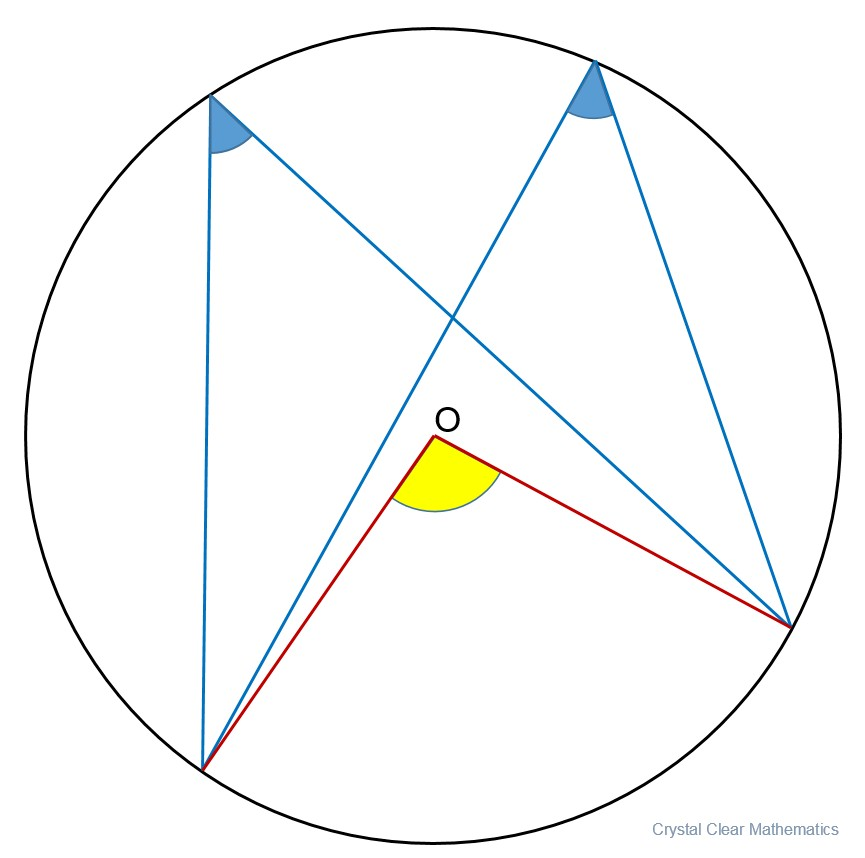
\includegraphics[scale=0.17]{FundamentalsPictures/CircleGeometry.jpg}}\\
In circle geometry, the inscribed angles are shown in blue and the central angle is shown in yellow.\\
Inscribed angles subtended by the same arc are equal.\\
The central angle is twice as large as the inscribed angle.

\subsubsection{Transformations}
\begin{itemize}
    \item Symmetry:\\
    A line of symmetry is an imaginary line that divides a shape into two identical parts. Shapes are symmetrical if they have at least one line of symmetry through them.
    \item Translations:\\
    Translations are the movement of a figure from one place to another; they don't change their size, arrangement, or direction.
    \item Rotations:\\
    Rotations are when objects turn in a circular motion around a fixed pivot point. The figure remains the same, as does each point's distance from the point of rotation
    \item Reflections:\\
    A reflection is a transformation that acts like a mirror: it swaps all pairs of points that are on exactly opposite sides of the line of reflection.
    \item Dilations:\\
    A dilation is a type of transformation that changes the size of the figure. The scale factor measures how much larger or smaller the image is. The angles remain the same.
    \item Congruence:\\
    Shapes are congruent with another if they are the same size and shape (same angles). Transformations can be applied to similar shapes to see if they can become congruent.
    \item Similarity:\\
    Two shapes are similar if a series of transformations can be applied to one in order to achieve the other. Similar shapes will always have matching angles.
\end{itemize}

\subsubsection{3D Shapes}
The volume of a shape is the 3D space that the object takes up.\\
The surface area is the sum of the areas of the shape's exterior.
Common 3D shapes:
\begin{itemize}
    \item A cube has all equal side lengths and equal square faces.
    $$V=l^3$$
    $$SA=6l^2$$
    \item A prism has two identical faces on each end, connected by a straight body.
    $$V=A_{base}h$$
    \item A pyramid has the vertices at the base come together to form a point above the base. Note that a cone is a special type of pyramid with a circular base.
    $$V=\frac{1}{3}A_{base}$$
    \item A sphere is entirely circular.
    $$V=\frac{4}{3}\pi r^2$$
    $$SA=4\pi r^2$$
\end{itemize}








\subsection{Arithmetic with Variables}

\subsubsection{Equations and Inequalities}
In an equation, one side must of the equation must always be equal to the other side. So what you do to one side, you must do to both sides. The only exception to this rule is if you are doing something to one side that doesn't change the overall value, such as adding 0 or multiplying/dividing by 1.\\
Equations are often used to solve for an unknown.\\
Ex: $3x-6=7x+2$
\begin{flalign*}
& 3x-6-2=7x+2-2 &\\
& 3x-8=7x &\\
& 3x-8-3x=7x-3x &\\
& -8=4x &\\
& \frac{-8}{4}=\frac{4x}{4} &\\
& -2=x &
\end{flalign*}
Inequalities are stating when one side is larger than the other side.\\
Ex: $3x>6\Rightarrow x>2$\\
Note that when multiplying both sides by a negative, the sign switches directions.\\
Ex: $-x>4\Rightarrow x<-4$

\subsubsection{Like Terms}
A term is a group that is linked together through multiplication or division operations. For example, $3x$ would be a term. Terms are broken up by addition and subtraction operations. Like terms are when two terms have the same combination of variables such as $3a$ and $2a$. These can be added or subtracted from each other as they both have the variable $a$ in common. In the case of $3a$ and $4b$, they are not like terms and cannot be combined. Also note that $x$ and $x^2$ are not like terms, as the one consists of a singular $x$ where as the other one consists of two.\\
Ex: $6a+4b+3a-2ab+b=9a+5b-2ab$

\subsubsection{Distributive Property}
This is when you multiply a number or variable on the outside of a pair of parentheses to each term on the inside.\\
Ex: $3(x+y)=3x+3y$\\
In general,
$$a(b+c)=ab+bc$$
The product of binomials is similar to the distributive property, when you multiply two or more groups in parentheses.
$$(a+b)(c+d)=ac+ad+bc+bd$$
Ex: $(x+1)(x-2)=x^2+x-2x-2=x^2-x-2$

\subsubsection{Factoring}
Factoring is the opposite of the distributive property. It's where you take out a common factor from a set of numbers and put them in brackets.\\
Ex: $3x+6=3(x+2)$\\
The first step is to factor out a GCF if possible. Sometimes this is all that can be done, as with binomials.\\
Trinomials can prove tricky.\\
Ex: $x^2+5x+6$\\
You need to find two numbers that add to get the middle term and multiply to get the constant (3rd term).\\
To do this, we can find the factor pairs of the constant.\\
So for this example, they are $\{1,6\},\,\{-1,-6\},\,\{2,3\},\,\{-2,-3\}$\\
We can then deduce that the pair $\{2,3\}$ will work, so the answer will be\\ ${x^2+5x+6=(x+2)(x+3)}$\\
If the coefficient of the first term is greater than 1, we instead find two numbers that multiply to get the constant times said coefficient and add to get the middle term.\\
Ex: $2x^2+x-3$\\
We find factor pairs of $-6$ which are $\{-1,6\},\,\{1,-6\},\,\{2,-3\},\,\{-2,3\}$\\
The pair is $\{-2,3\}$ so our answer is\\
$2x^2+x-3=(2x+3)(x-1)$







\subsection{Power Laws}

\subsubsection{Exponent Laws}
Product Rule: when multiplying two like variables, you add the exponents.\\ Ex: $x^2\cdot x=x^3$
$$a^x\cdot a^y=a^{x+y}$$
Quotient Rule: when dividing two like variables, you subtract the exponents.\\
Ex: $\frac{x^2}{x}=x$
$$\frac{a^x}{a^y}=a^{x-y}$$
Power Rule: when you have an exponent to a power, the two exponents multiply.\\
Ex: $(x^3)^2=x^6$
$$(a^x)^y=a^{xy}$$
Power of a Product Rule: the exponent of a product is applied to all factors.\\
Ex: $(xy)^2=x^2y^2$
$$(ab)^x=a^xb^x$$
Power of a Fraction Rule: same as the power of a product rule - it also applies to division.\\
Ex: $\left(\frac{x}{3}\right)^2=\frac{x^2}{9}$
$$\left(\frac{a}{b}\right)^x=\frac{a^x}{b^x}$$
Negative Exponents: if an exponent is negative, it takes the reciprocal of the number.\\
Ex: $x^{-2}=\frac{1}{x^2}$
$$a^{-x}=\frac{1}{a^x}$$
Fractional Exponent: If an exponent is in the form of a fraction, the numerator refers to the exponent of a number and the denominator refers to the root.\\
Ex: $x^{2/3}=(\sqrt[3]{x})^2$
$$a^{\frac{x}{y}}=\left(\sqrt[y]{a}\right)^x$$

\subsubsection{Simplifying Radicals}
As we have seen, radicals are a special type of exponent so we can apply the same rules.\\
Product of Radicals:
$$\sqrt[x]{a}\sqrt[x]{b}=\sqrt[x]{ab}$$
Quotient of Radicals:
$$\frac{\sqrt[x]{a}}{\sqrt[x]{b}}=\sqrt[x]{\frac{a}{b}}$$
Radical of a Radical:
$$\sqrt[x]{\sqrt[y]{a}}=\sqrt[xy]{a}$$
Using these rules, we can simplify certain radicals.\\
Ex: $\sqrt{20}$\\
We can break the radical up into its largest perfect square (or cube, or whatever the radical specifies).\\
$\sqrt{20}=\sqrt{4}\sqrt{5}$\\
Then we can take the definitive value of that perfect square, removing the radical.\\
So $2\sqrt{5}$ will be the simplified root.

\subsubsection{Rationalizing}
Sometimes we want to change the appearance of a fraction with a radical to make it easier to work with. We can do this by multiplying by 1 (or $\frac{a}{a}$).\\
Ex: $\frac{1}{\sqrt{3}}=\frac{1}{\sqrt{3}}\left(\frac{\sqrt{3}}{\sqrt{3}}\right)=\frac{\sqrt{3}}{3}$\\
This becomes more complicated if we are dealing with a binomial. In this case we will need to multiply by the conjugate of the denominator. The conjugate of a binomial is where the second term of the binomial switches signs.\\
Ex: conjugate of $x+3$ is $x-3$.\\
Now let's use the conjugate to simplify a binomial fraction.\\
Ex: $\frac{1}{x+\sqrt{2}}=\frac{1}{x+\sqrt{2}}\left(\frac{x-\sqrt{2}}{x-\sqrt{2}}\right)=\frac{x-\sqrt{2}}{x^2-2}$







\subsection{Trigonometric Ratios}

\subsubsection{Right Angle Trigonometry}
\centerline{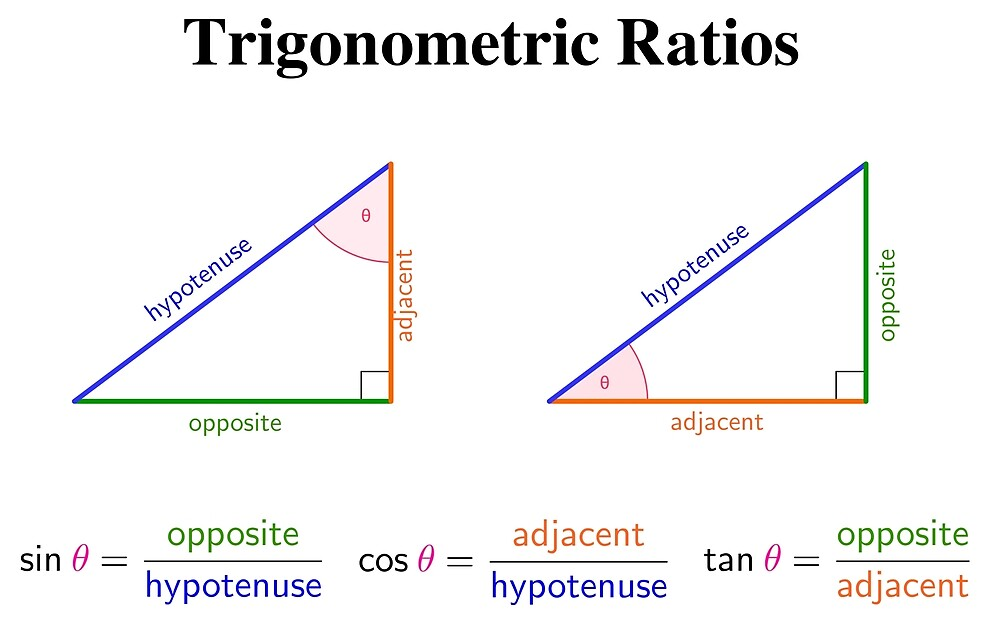
\includegraphics[scale=0.3]{FundamentalsPictures/TrigRatios.jpg}}
Hypotenuse is the lonest end of the triangle.\\
Opposite is the side across from the angle in question.\\
Adjacent is the side next to the angle in question.\\
Note these ratios only work for right angle triangles.\\
\\
Special Triangles:\\
Often we need a calculator to determine the numeric value of the side lengths. There are two useful triangles that we use that allows us to compute the trig ratios without using a calculator. These are called special triangles.\\
\centerline{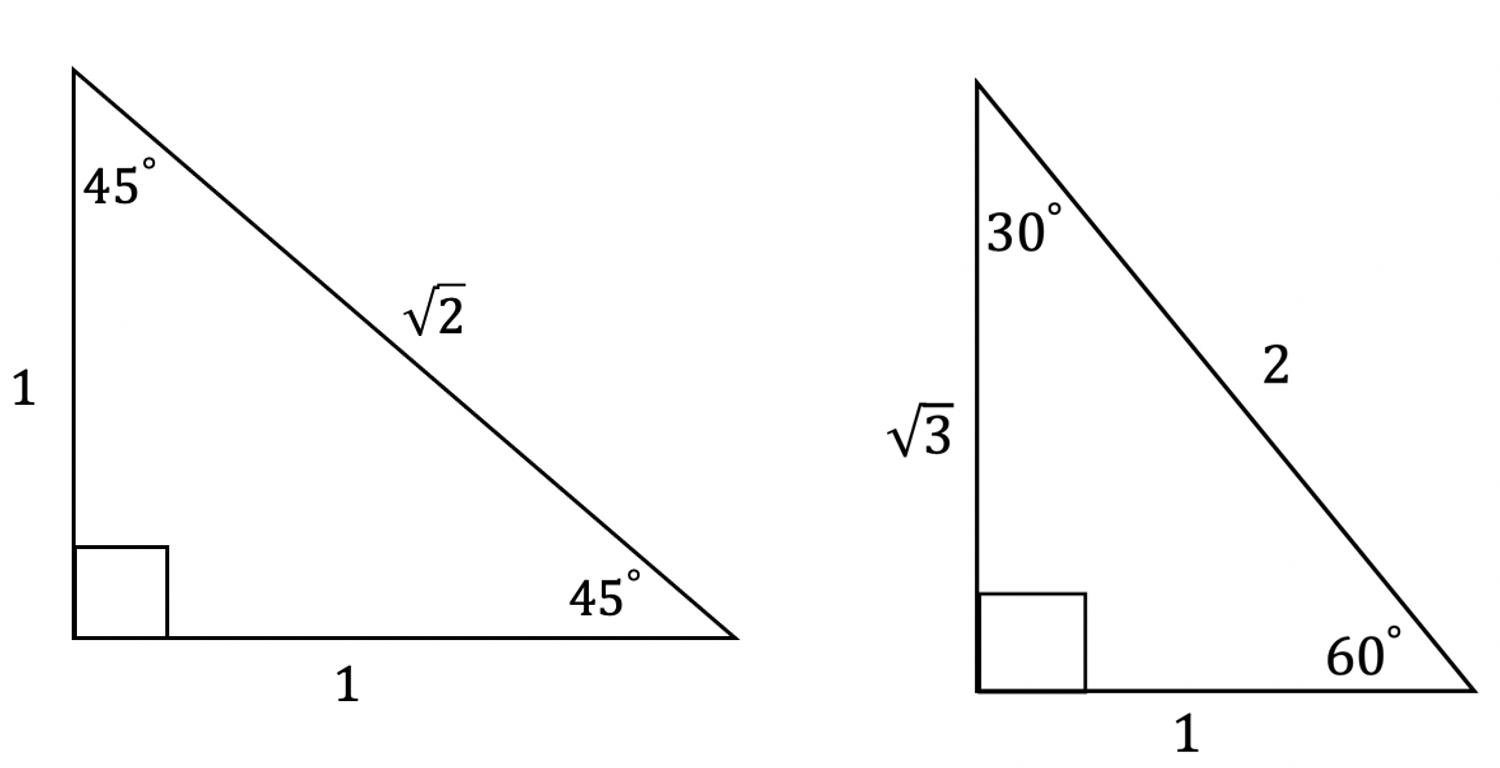
\includegraphics[scale=0.5]{FundamentalsPictures/SpecialTriangles.png}}

\subsubsection{Sine and Cosine Law}
\centerline{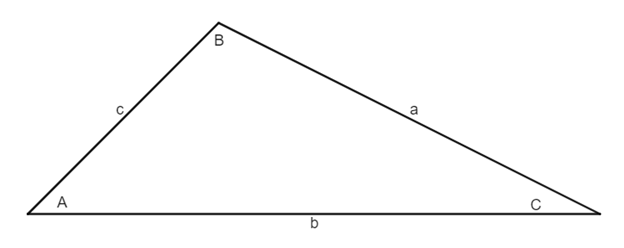
\includegraphics[scale=0.7]{FundamentalsPictures/SineLawTriangle.png}}
The cosine law is an extension of Pythagorean's theorem for all triangles (not just right angled ones).
$$c^2=a^2+b^2-2ab\cos C$$
Note that the usage of $a$, $b$, and $c$ is interchangeable.\\
\\
The sine law is a relationship between the ratio of sides and angles in any triangle.
$$\frac{\sin A}{a}=\frac{\sin B}{b}=\frac{\sin C}{c}$$









\subsection{Sequences and Series}

\subsubsection{Summation Notation}
Summation notation is a shorthand was to express the sum of a set of numbers. The bottom of the sigma tells you what index to start at and the top of the sigma tells you which number to end at.\\
Ex: $\sum \limits_{x=1}^5 x=1+2+3+4+5=15$\\
We can use similar notation for repeated multiplication as well. For this we use an upper case pi and use the same notation, using the starting point, stopping point, and index.\\
Ex: $\prod \limits_{x=2}^4=2\cdot 3\cdot 4=24$

\subsubsection{Arithmetic Sequence}
A sequence is an ordered list of numbers. Each number in the list is referred to as an element or term. Each new term follows a pattern or rule to determine the next term in the sequence.\\
An arithmetic sequence is an ordered list of terms in which the difference between consecutive terms is constant. It is generally expressed as $\{a,a+d,a+2d,a+3d,\ldots\}$\\ The formula for the nth term of the sequence is given by,
$$t_n=a+(n-1)d$$
where $a$ is the first term, $d$ is the common difference between consecutive terms, and n is the term number.

\subsubsection{Arithmetic Series}
An arithmetic series is the sum of all terms that form an arithmetic sequence. $S_n$ represents the sum of the first $n$ terms of a series.
$$S_N=\frac{N}{2}(a+t_N)=\frac{N}{2}(2a+(N-1)d)=\sum \limits_{n=1}^N (a+(n-1)d)$$

\subsubsection{Geometric Sequence}
Geometric sequences are sequences in which the ratio of consecutive terms is constant. The common ratio, $r$, can be found by taking any term, except for the first, and dividing that term by the preceding term.\\
The general geometric sequence is $\{a,ar,ar^2,ar^3,\ldots\}$\\
The general term for a geometric sequence is,
$$t_n=ar^{n-1}$$
where $a$ is the first term and $r$ is the common ratio.

\subsubsection{Geometric Series}
A geometric series is the expression for the sum of the first $N$ terms of a geometric sequence. It is expressed as,
$$S_N=\frac{a(r^n-1)}{r-1}=\frac{rt_n-a}{r-1}=\sum \limits_{n=1}^N ar^{n-1}$$
As the number of terms in the series gets increasingly large, it will either approach an infinite value or a fixed and finite value. The series comes to a fixed value for $|r|<1$. This infinite series can be computed as,
$$S_\infty=\frac{a}{1-r}$$








\subsection{Analyzing Data}
\subsubsection{Displaying Data}
If we have the table:\\

\begin{tabular}{c|c|c|c|c}
    Drink & Type & Calories & Sugar (g) & Caffeine (mg)\\
    \hline
    coffee & hot & 4 & 0 & 260\\
    latte & hot & 100 & 14 & 75\\
    mocha & hot & 170 & 27 & 95
\end{tabular}\\
The \textit{individuals} are defined to be the drinks in this case (the things we are collecting data from).\\
There are also 4 variables. The variable "Type" is \textit{categorical}, meaning that the data it holds fits into one of some number of categories (digital vs. analog).\\
Some types of graphs we can use to represent data includes pictographs, bar graphs, frequency graphs, pie graphs, and many more.\\
Ex: Bar graph\\
\centerline{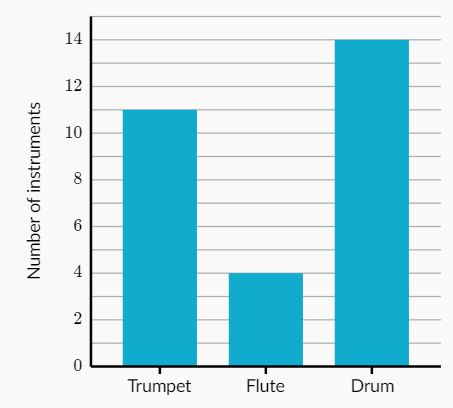
\includegraphics[scale=0.7]{FundamentalsPictures/barGraph.png}}
Data that relates to itself, we can represent with a two-way table.\\
Ex: Say we have 10 candies, 6 chocolate, 3 chocolate-coconut, 1 coconut, and 2 plain. We can express this as\\
\begin{tabular}{c|c|c}
    & Coconut & No Coconut\\
    \hline
    Chocolate & 3 & 6\\
    No Chocolate & 1 & 2
\end{tabular}\\
A two-way table with relative frequencies is when the columns are normalized to equal 1.\\
\begin{tabular}{c|c|c}
    & Coconut & No Coconut\\
    \hline
    Chocolate & 75\% & 75\%\\
    No Chocolate & 25\% & 25\%
\end{tabular}\\
\textit{Conditional distribution} is when you analyze a single row/column or a subset of the table.\\
\textit{Marginal distribution} is when you analyze the totals of the rows/columns.\\
Frequency plots are similar to bar graphs but are more all-encompassing. We can use frequency graphs to represent data that is more analog than discrete, called a histogram.\\
Ex:\\
\centerline{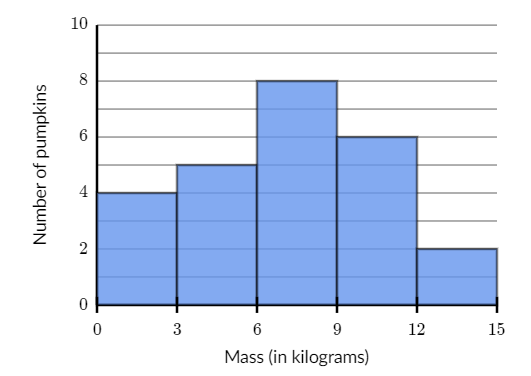
\includegraphics[scale=0.7]{FundamentalsPictures/histogram.png}}
With histograms we can classify different behaviors of the data.\\
The maximum value of the histogram is the \textit{peak}.\\
If there are groupings of data points in a similar area, we call those \textit{clusters}\\
If there are a small number of data points far away from the majority of the data, we call those \textit{outliers}.\\
We can also represent frequency data using a stem-leaf plot.\\
Ex:\\
\begin{tabular}{c|l}
    Stem & Leaf\\
    \hline
    0 & 0, 0, 2, 4, 7, 7, 9\\
    1 & 1, 1, 3, 8\\
    2 & 0
\end{tabular}\\
maps to the data 0, 0, 2, 4, 7, 7, 9, 11, 11, 13, 18, 20.\\
The stem maps the tens place value and the leaf maps the ones place value

\subsubsection{Center and Spread}
The average of a set of data is a measure of central tendency of that data and there are many ways to express the average.\\
The \textit{mean} is the arithmetic sum of the data divided by the number of data points
$$\mu=\frac{1}{N}\sum_{i=1}^N x_i$$
The \textit{median} is the middle value of the data set. If there are an even number of data points, the median is the mean of the two middle data points.\\
The \textit{mode} is the most commonly occurring value.\\
The \textit{midrange} is the mean of the difference between the maximum and minimum values in the data set.\\

Mean is the standard measure for average in most cases, though it is important to note that outliers can sometimes have a large, unwanted, effect on the mean so in these cases, it may be best to use median as the average.\\

Data sets can have the same averages but may look very different. To represent this, we introduce spread. Spread is how spread out the data points are.\\
The most simple measure of spread is the \textit{range} which is simply the difference between the maximum and minimum values in the data set.\\
A slightly more elaborate method of calculating spread is the \textit{mean absolute deviation} (MAD). This is the mean of how far away a number is from the mean.
$$MAD=\frac{1}{N}\sum_{i=1}^N|x_i-\mu|$$
The \textit{interquartile range} (IQR) is analogous to the median of a data set. The IQR is the difference between the 1st and 3rd quartiles in a data set. The first quartile is the median of the lower half of the data and the 3rd quartile is the median of the higher half of the data.\\
Ex: For data of 1,3,3,3,4,4,4,6,6,\\
Median$=4$\\
$Q_1=\text{median}\brcurly{1,3,3,3}=3$\\
$Q_3=\text{median}\brcurly{4,4,6,6}=5$\\
IQR$=5-3=2$\\
We can use the IQR to represent data as a box and whisker plot:\\
\centerline{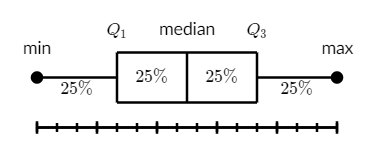
\includegraphics[scale=1]{FundamentalsPictures/boxPlot.png}}\\
We can also use the IQR to define outliers. We can use the general rule of 1.5 times the IQR. Any outliers can be defined to be less than $Q_1-1.5\cdot IQR$ or greater than $Q_3+1.5\cdot IQR$\\
\textit{Variance} is the mean of the squared distance between the value and the mean, represented by $\sigma^2$
$$\sigma^2=\frac{1}{N}\sum_{i=1}^N (x_i-\mu)^2$$
By expanding the quadratic and using the definition of the mean, we can also write this as
$$\sigma^2=\frac{1}{N}\sum_{i=1}^N x_i-\mu^2$$
The \textit{standard deviation} is the square root of the variance.
$$\sigma=\sqrt{\frac{1}{N}\sum_{i=1}^N (x_i-\mu)^2}$$
We can use the standard deviation to calculate Z-scores. A Z-score is how many standard deviations a data point is from the mean.
$$Z_i=\frac{x_i-\mu}{\sigma}$$
In an ordered list of data, we can calculate the percentile by dividing the position of the data point by the number of data points in the sample size. Note that the median corresponds to the 50th percentile. Z-scores are particularly useful in calculating percentiles as we can use the aid of Z-tables to compute percentiles along a normal distribution.






\subsection{Probability and Combinatorics}

\subsubsection{Probability}
Probability is the likelihood of an event occurring. (the number of possibilities that satisfy a given constraint over the number of possible outcomes)\\
Probability is always expressed as a number between $0$ and $1$.\\
The probability of an event, $A$, is denoted by $P(A)$.\\
The sum of all possibilities of an event is equal to $1$.\\
Relative frequency is the frequency of an event occurring in a trial to provide an estimate of the probability. Note that the more trials, the better the estimate will be.\\
\\
Definitions:
\begin{itemize}
    \item Two events are mutually exclusive if they cannot occur at the same time.
    \item The probability of event $A$, given event $B$, is called conditional probability. $P(A|B)$ is conditional probability of $A$, given $B$.
    \item The intersection of two events is the likelihood of both events occurring. It is the set of elements that are common to both events. Denoted by $P(A\cap B)$
    \item The union of two events is the probability of at least one of the events occurring. Denoted by $P(A\cup B)$
    \item Independent Events: The probability of $A$ does not affect the probability of $B$.
    \item Dependent Events: Occurrence of event $A$ changes the probability of event $B$ occurring.
    \item The compliment of an event is the case of an event not occurring. $P(A')$ is the probability that $A$ does not occur.
\end{itemize}
Rules of Probability:
\begin{align*}
    &P(A)+P(A')=1\\
    &P(A\cap B)=P(A)P(B|A)\\
    &P(A\cup B)=P(A)+P(B)-P(A\cap B)
\end{align*}

\subsubsection{Combinatorics}
Consider a task made up of several stages. The number of choices for the first stage is $a$, the number for the second stage is $b$, then $c$ and so on. The number of ways the task can be completed (or the number of possible outcomes) is: $a\cdot b\cdot c\cdot d\cdots$\\
Ex: using the letters $A, B, C,D,E,F$, how many 4 letter combinations can be made if:\\
a) letters can be repeated?\\
b) letters can not be repeated?\\
a) $6\cdot6\cdot6\cdot6=6^4=1296$\\
b) $6\cdot5\cdot4\cdot3=360$\\
\\
Factorial Notation:\\
The symbol '!' indicates factorial and means the product of decreasing natural numbers
$$n!=n(n-1)(n-2)\cdots3\cdot2\cdot1=\prod_{i=1}^ni$$
Ex: Simplify $\dfrac{25!}{23!5!}$
\begin{align*}
    \frac{25\cdot24\cdot23!}{23!5\cdot4\cdot3\cdot2\cdot1}=\frac{25\cdot24}{5\cdot4\cdot3\cdot2}=5
\end{align*}
Ex2: Simplify $\dfrac{(n+1)!}{(n-1)!}$
\begin{align*}
    \frac{n+1)(n)(n-1)!}{(n-1)!}=n(n+1)
\end{align*}
\\
Permutations:\\
A permutation is an arrangement of distinct objects in which the order is important.\\
The number of permutations of $n$ distinct objects is $n!$\\
The number of permutations of $n$ distinct objects taken $r$ at a time is:
$$\prescript{}{n}{P}_r=\frac{n!}{(n-r)!}$$
Ex: licence plates have 3 digits followed by 3 letters. How many different plates can be made?\\
\begin{align*}
    \perm{10}{3}\perm{26}{3}=\frac{10!}{(10-3)!}\frac{26!}{(26-3)!}=11232000
\end{align*}
Ex2: Solve for $n$ if $\perm{n}{2}=30$
\begin{align*}
    &\frac{n!}{(n-2)!}=30\\
    &\frac{n(n-1)(n-2)!}{(n-2)!}=30\\
    &n^2-n=30\\
    &n^2-n-30=0\\
    &(n-6)(n+5)=0\\
    &\Ra n=6,\,n=-5\\
    &n\neq-5\text{ because }n\in\mathbb{N}\\
    &\therefore n=6
\end{align*}
Some permutations have restrictions where certain objects must be grouped. If objects are grouped together, the number of possible outcomes can be calculated by multiplying:\\
(total number of groups or individuals)!(number in group 1)!(number in group 2)!$\cdots$\\
Ex: How many ways can "PICTURE" be arranged if:\\
a) two vowels must be together?\\
b) A vowel cannot be beside another vowel?\\
\\
a) This forms 6 groups with one group of two so $6!2!=1440$\\
b) For this one we can calculate it by taking the total arrangements, $7!$, and subtracting the arrangements that don't fit the criteria.\\
3 vowels together: $5!3!$\\
2 vowels together: $6!2!$\\
So the answer will be: $7!-5!3!-6!2!=280$\\
\\
If there are repetitions, the number of permutations can be expressed as $\dfrac{n!}{a!b!c!\cdots}$ where $a$, $b$, and $c$ are the number of repetitions for each identical object\\
Ex: a true-false quiz has 10 questions. How many answer keys are possible if 4 are true and 6 are false?\\
$\dfrac{10!}{6!4!}=210$\\
\\
Combinations:\\
A combination is an arrangement of distinct objects in which the order of the objects is not important.
$$\comb{n}{r}=\frac{\perm{n}{r}}{r!}=\frac{n!}{r!(n-r)!}=\left(\begin{matrix} n\\r\end{matrix}\right)$$
Ex: Looking at a 5-card hand in a deck of cards:\\
a) how many 5 card hands are there?\\
b) how many with all hearts?\\
c) how many with 3 hearts and 2 spades?\\
d) how many with at most 3 hearts?\\
\\
a) $\comb{52}{5}=2598960$\\
b) $\comb{13}{5}\comb{39}{0}=1287$\\
c) $\comb{13}{3}\comb{13}{2}\comb{39}{0}$\\
d) We can sum all the different possibilities
\begin{align*}
    &\text{3 hearts: }\comb{13}{3}\comb{39}{2}\\
    &\text{2 hearts: } \comb{13}{2}\comb{39}{3}\\
    &\text{1 heart: }\comb{13}{1}\comb{39}{4}\\
    &\text{0 hearts: }\comb{13}{0}\comb{39}{5}\\
    &\text{Total is }2569788
\end{align*}

\subsubsection{Pascal's Triangle}
\centerline{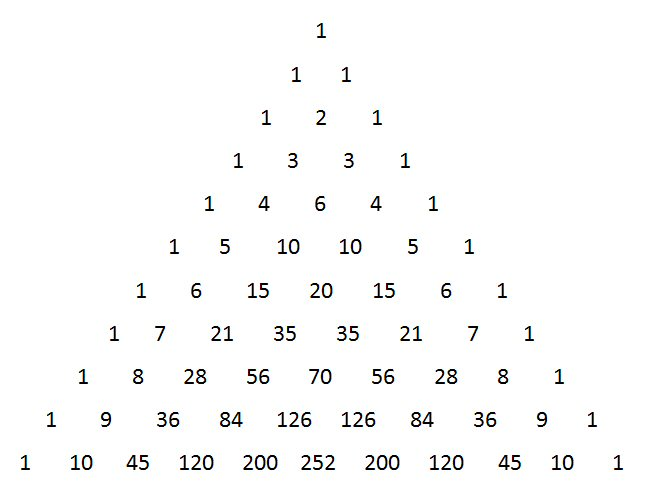
\includegraphics[scale=0.5]{FundamentalsPictures/PascalTriangle.jpg}}
It can also be written using combinations for where $n$ is the row number and $r$ is the term number where we start counting from 0.\\
\centerline{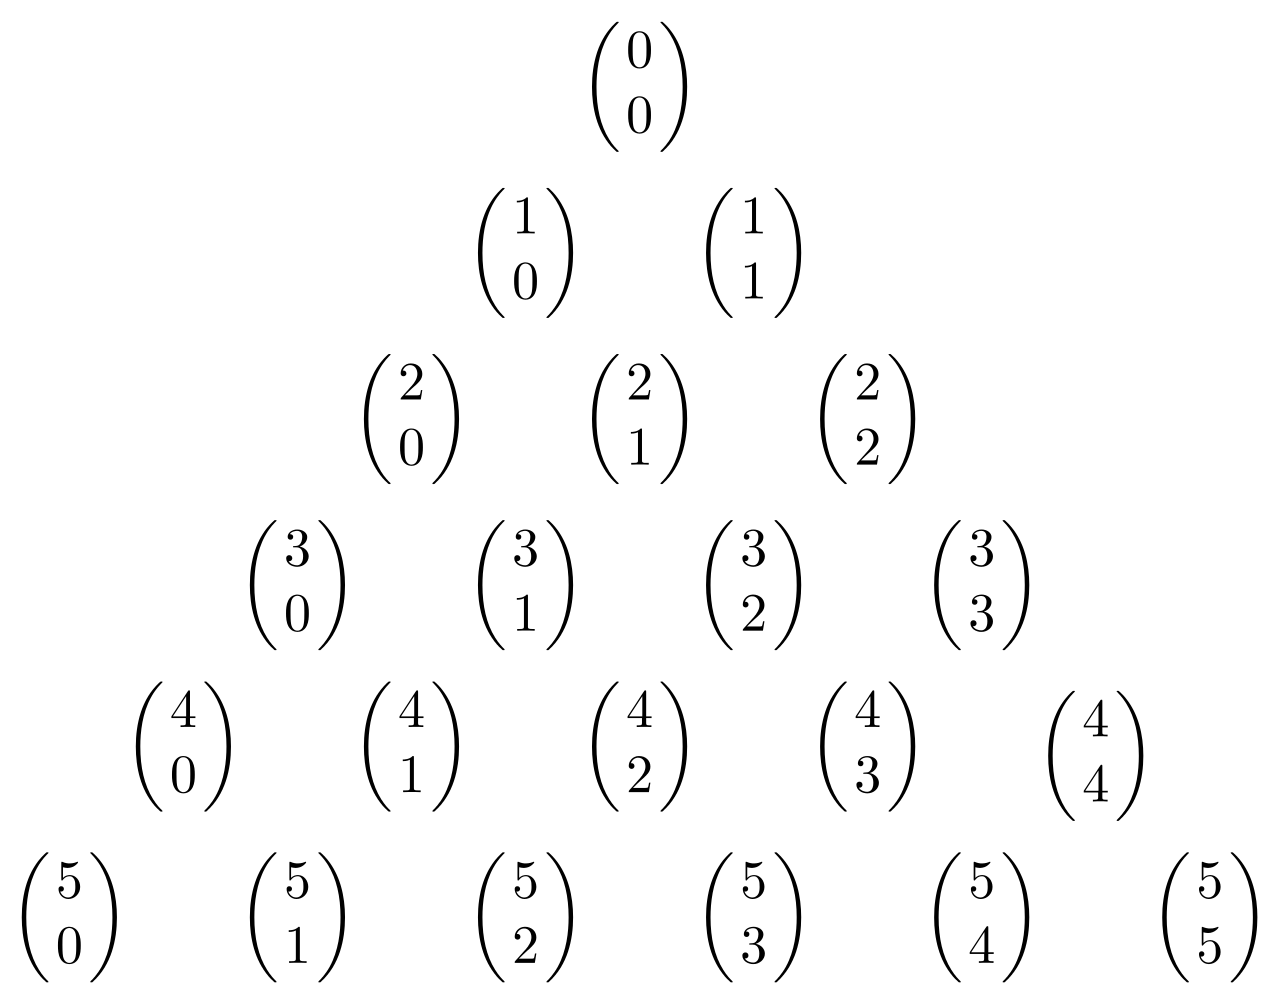
\includegraphics[scale=0.2]{FundamentalsPictures/PascalTriangleComb.png}}\\
The sum of each row can be expresses by the geometric sequence $t_n=2^{n-1}$ where $n$ is the row number and $t_n$ is the sum of that row.\\
\\
Pathway Problems:\\
Another occurrence of Pascal's triangle is if we want to find the number of different possible pathways to travel to a point on a grid.\\
\centerline{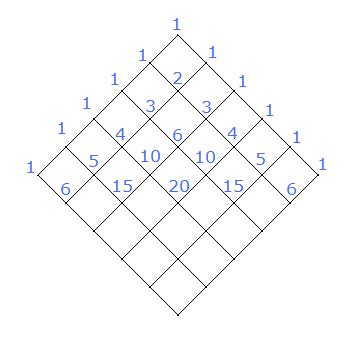
\includegraphics[scale=0.55]{FundamentalsPictures/PascalTrianglePathway.png}}
For a simple grid as shown, we can find the number of pathways using permutations.\\
For the 5x5 grid, we go down 5 moves and right 5 moves for a total of 10 moves. So we can express it as $\dfrac{10!}{5!5!}=252$ moves.\\
Note that this only works for perfect grids. A more difficult example, we need to use the general process of Pascal's triangle and sum adjacent corners to come to the answer.\\
Ex:\\
\centerline{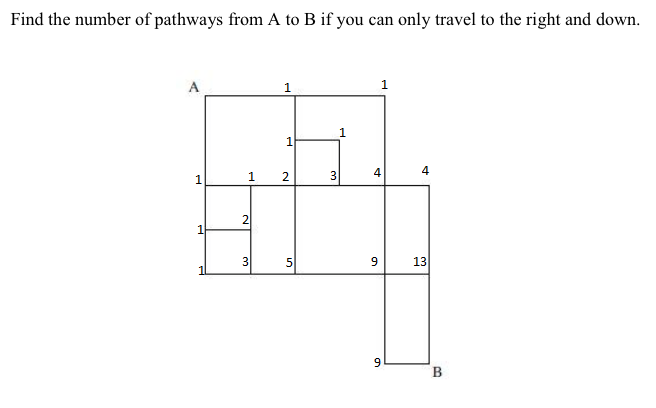
\includegraphics[scale=0.8]{FundamentalsPictures/PathwayEx.png}}
So there will be a total of 22 different paths between A and B.\\
\\
The Binomial Theorem:\\
This is used to expand any power of a binomial expression $(a+b)^n$\\
It follows the patterns of Pascal's triangle and can be expressed as:
$$(a+b)^n=\comb{n}{0}(a)^n(b)^0+\comb{n}{1}(a)^{n-1}(b)^1+\comb{n}{2}(a)^{n-2}(b)^2+\cdots+\comb{n}{n-1}(a)^1(b)^{n-1}+\comb{n}{n}(a)^0(b)^n$$
$$(a+b)^n=\sum_{k=0}^n\left(\begin{matrix}n\\k\end{matrix}\right)a^{n-k}b^k$$

































% Elementrary Logic

\section{Introductory Logic}
\subsection{Arguments}
\subsubsection{Introduction to Arguments, Fallacies, and Logic}
Familiar types of logic:
\begin{itemize}
    \item Quarrels
    \item Legislative debates
    \item Labour negotiations
    \item Diplomatic discussions
    \item Legal arguments
    \item Mathematical proofs
    \item Scientific demonstrations
\end{itemize}
Arguments in the broad sense:
\begin{itemize}
    \item attempt to build a case in favour of some claim
    \item involve the presentation of reasons or evidence (premises) in support of a conclusion
    \item are social exchanges often involving a series of speech acts uttered by two or more parties
    \item are governed by a set of rules or standards (sometimes implicit)
    \item attempt to advance knowledge by justifying or undermining a conclusion
\end{itemize}
Arguments in the narrow sense are sets of propositions composed of an argument's \textit{premises} and \textit{conclusion}.\\
Logic, understood broadly, studies arguments in the broad sense.
Logic, understood narrowly, studies arguments in the narrow sense.\\

\textbf{Placing Arguments in Standard Form}
Ex: Archimedes must be either a hero or a martyr. After all, anyone who dies in battle is one or the other. And, as we know, Archimedes perished during the capture of Syracuse.\\

\begin{tabular}{p{16cm}}
\textbf{Premise 1:} Anyone who dies in battle is either a hero or a martyr\\
\textbf{Premise 2:} Archimedes perished during the capture of Syracuse\\
\hline
\textbf{Conclusion:} Therefore, Archimedes must be either a hero or a martyr
\end{tabular}\\

How to place an argument in standard form:
\begin{enumerate}
    \item Identify the premises and conclusion
    \item Eliminate any unnecessary or redundant words or phrases
    \item Clarify any ambiguities
    \item Separate the premises from the conclusion with a horizontal line
\end{enumerate}

How to Handle Sub-Arguments\\
You could display as one argument or display as separate arguments with the conclusion of the sub-argument becoming a premise of the main argument\\
Ex2: If Bill wants to live in Auckland, then he has to learn to sail. If Bill has to learn to sail, then he will have to learn navigation. It turns out that Bill does want to live in Auckland. So Bill will have to learn navigation.\\

Displayed as one argument:\\
\begin{tabular}{p{16cm}}
    \textbf{Premise: }If Bill wants to live in Auckland, then he has to learn to sail\\
    \textbf{Premise: }If Bill has to learn to sail, then he has to learn navigation\\
    \textbf{Premise: }Bill wants to live in Auckland\\
    \hline
    \textbf{Conclusion: }Therefore, Bill has to learn navigation.
\end{tabular}\\

Displayed as two arguments:\\
\begin{tabular}{p{16cm}}
    \textbf{Premise: }If Bill wants to live in Auckland, then he has to learn to sail\\
    \textbf{Premise: }Bill wants to live in Auckland\\
    \hline
    \textbf{Intermediate Conclusion: }Bill has to learn to sail.
\end{tabular}\\

\begin{tabular}{p{16cm}}
    \textbf{Premise: }If Bill has to learn to sail, then he has to learn navigation\\
    \textbf{Premise: }Bill has to learn to sail.\\
    \hline
    \textbf{Conclusion: }Therefore, Bill has to learn navigation.
\end{tabular}\\

Ex3: Geometry should not include lines that are strings, in that they are sometimes straight and sometimes curved, since the ratios between straight and curved lines are not known, and I believe cannot be discovered by human minds, and therefore no conclusion based upon such ratios can be accepted as rigorous and exact. [Rene Descartes]\\

\begin{tabular}{p{16cm}}
    The strings are sometimes straight and sometimes curved\\
    The ratios between straight and curved lines are not known and cannot be discovered by human minds\\
    \hline
    No conclusion based upon the ratios between straight and curved lines can be accepted as rigorous and exact
\end{tabular}\\

\begin{tabular}{p{16cm}}
    No conclusion based upon the ratios between straight and curved lines can be accepted as rigorous and exact\\
    \hline
    Geometry should not include lines that are strings
\end{tabular}\\

\textbf{Identifying Propositions}
Propositions are
\begin{itemize}
    \item bearers of truth (either true/false)
    \item distinct from questions (interrogatives), commands (imperatives), prayers, etc.
    \item usually expressed by statements (declarations), but sometimes also by other means, e.g. rhetorical questions
\end{itemize}
Ex: Sue is visiting Hong Kong.\\
is a proposition\\
Ex2: When is Bill's birthday?\\
not a proposition\\
Ex3: Who doesn't know London is a great city?\\
This is a rhetorical question stating that London is a great city\\
so it is a proposition\\

\textbf{Indicator Words or Phrases for Conclusions}
\begin{itemize}
    \item thus
    \item hence
    \item therefore
    \item consequently
    \item which implies that
    \item so
    \item it follows that
    \item for this reason
    \item we may conclude that
    \item which proves that
\end{itemize}
\textbf{Indicator Words or Phrases for Premises}
\begin{itemize}
    \item because
    \item as
    \item since
    \item moreover
    \item given that
    \item provided that
    \item assuming that
    \item on the grounds that
\end{itemize}

\textbf{Evaluating Arguments}
The quality of an argument depends on
\begin{itemize}
    \item the truth of the argument's premises
    \item the strength of the consequence relation that holds between the arguments premises and conclusion
\end{itemize}
Two main ways to criticize an argument are
\begin{itemize}
    \item to show that the premises are (likely) not true
    \item to show that the consequence relation is (likely) not strong
\end{itemize}
\textbf{Consequence Relations}
\begin{itemize}
    \item If the premises of an argument, when assumed to be true, provide good evidence in favour of that argument's conclusion, the argument has a strong consequence relation
    \item If the premises of an argument, when assumed to be true, provide poor evidence in favour of that argument's conclusion, the argument has a weak consequence relation
    \item A consequence relation that is neither strong nor weak is moderate
\end{itemize}
Ex: Strong\\
\begin{tabular}{p{16cm}}
    Socrates is a father\\
    \hline
    Therefore Socrates is male
\end{tabular}\\
Ex2: Moderate\\
\begin{tabular}{p{16cm}}
Plato lives in Athens\\
\hline
Therefore Plato is Greek
\end{tabular}\\
Ex3: Weak\\
\begin{tabular}{p{16cm}}
Aristotle is male\\
\hline
Therefore Aristotle is a father
\end{tabular}\\

\textbf{Deductive Arguments}\\
A \textit{deductive argument} is one presented with the intention of being judged by \textit{deductive standards}.\\
An argument meets the standard of deductive adequacy only when it is impossible for its conclusion to be false, assuming that its premises are all true.\\
The consequence relation is as strong as it can get.\\

\textbf{Inductive Arguments}\\
An \textit{inductive argument} is one presented with the intention of being judged by \textit{inductive standards}.\\
An argument meets the standard of inductive adequacy only when it is not deductively adequate and its premises, if true, increase the likelihood of its conclusion also being true.\\
Ex: Deductive vs. inductive\\
Deductive:\\
\begin{tabular}{p{16cm}}
Russell had a brother\\
\hline
Russel had a sibling
\end{tabular}\\

Inductive:\\
\begin{tabular}{p{16cm}}
Russell had a sibling\\
\hline
Russell had a brother
\end{tabular}\\

\textbf{Logic vs. Rhetoric}\\
Rhetoric:
\begin{itemize}
    \item studies arguments that are \textit{in fact} persuasive
    \item is defined as the science of persuasion
\end{itemize}
Logic:
\begin{itemize}
    \item studies arguments that \textit{ought to be} persuasive or that would be persuasive to an ideally rational agent.
    \item is defined as the science of reasoned (or rational) persuasion.
\end{itemize}

\subsubsection{Types of Arguments}
\textbf{The Quarrel}
\textbf{The ``Yes, you did," "No, I didn't" Quarrel}\\
Sue: I thought you told me that you were going to be at the library last Friday.\\
Bill: No. Don't you remember? I said I would be at the beach.\\
Sue: No. You said you would be at the library. Otherwise I would have wanted to go with you.\\
Bill: You're not remembering things correctly—that was the day I said I would be at the beach!\\

Bill and Sue disagree about what the facts are. They disagree what premises they share. They have \textit{promissory instability}.\\

\textbf{The``You don't love me anymore" Quarrel}\\
Bill: You don't love me.\\
Sue: But I do! How could I call you a "mindless bore" without caring for you enough to risk giving offense, perhaps even losing you?\\
Bill: Sure, sure. How do I know that this isn't just what you have in mind—losing me, as you call it, or breaking up, as I would say?\\
Sue: Bill, you just don't understand. Be reasonable.\\

Bill and Sue agree about the facts but they disagree about what the facts imply. Bill and Sue disagree about what conclusions they should draw. They have \textit{conclusional instability}.\\

\textbf{Definition}:\\
A \textit{quarrel} is any argument in which:
\begin{itemize}
    \item the disputants suffer from premissory or conclusional instability (or both)
    \item lack of a shared method for conflict resolution
    \item refure to agree to disagree
\end{itemize}

\textbf{Fallacies}
A \textit{fallacy} is:
\begin{itemize}
    \item a bad argument or inference that has a propensity to appear good
    \item a common or seductive error in reasoning
\end{itemize}
Ex: The press should print all news that is in the public interest. The public interest in this murder case is intense. Therefore, the press should print news about this case.\\

Note that the argument involves an ambiguous phrase "public interest" (meaning "of benefit to the public" versus "of interest to the public"). This is called an \textit{equivocation}.

\textbf{The Ad Baculum}
An \textit{ad baculum} argument occurs whenever a conclusion is drawn on the basis of an appeal to force, intimidation, or threat of bad consequences.\\
If the appeal is relevant, it is non-fallacious\\
If the appeal is irrelevant, it is fallacious\\

Ex: Our paper certainly deserves the support of every German. We shall continue to forward copies of it to you, and hope that you will not want to expose yourself to unfortunate consequences in the case of cancellation.\\

This does not recommend any explicit belief so it is not fallacious.
\begin{itemize}
    \item If an argument is about what is sensible or prudent to \textit{do}, the argument is not fallacious
    \item If an argument is about what is sensible or rational to \textit{believe}, the argument is fallacious.
\end{itemize}

Ex:2 ``Toyota Motor said will build a new plant in Baja, Mexico, to build Corolla cars for U.S. NO WAY! Build a plant in U.S. or pay big border tax." [Donald Trump, 2017]\\
Not fallacious.\\

Ex3: Zach: ``My father owns the department store that gives your newspaper forty percent of your advertising revenue, and my understanding is that you don't want to publish any story of my arrest for spray painting the college."\\
Newspaper editor: ``Yes, Zach, I see your point. The story doesn't seem to be newsworthy.\\

Whether or not the story deserves the attention of the public needs to be judged by some other criteria, not the ones given by Zach, thus the argument is fallacious.\\

Ex4: Zach: ``My father owns the department store that gives your newspaper forty percent of your advertising revenue, and my understanding is that you don't want to publish any story of my arrest for spray painting the college."\\
Newspaper editor: ``Yes, Zach, I see your point. Looks like we shouldn't do it lest we all lose our jobs, indeed.\\

As a consideration of what the newspaper should do in order to avoid the bad consequences, the appeal is highly relevant, this non-fallacious argument.\\

\textbf{The Ad Hominem}
An ad hominem argument occurs whenever a conclusion is drawn on the basis of an appeal to some fact or alleged fact about one's opponent.\\
If the appeal is relevant, the argument is non-fallacious\\
If the appeal is irrelevant, the argument is fallacious\\

There are two main types of ad hominem
\begin{itemize}
    \item the \textit{abusive ad hominem}, in which an insulting or unwelcome allegation is advanced about one's opponent
    \item the \textit{circumstantial ad hominem}, in which a non-abusive allegation is advanced about one's opponent, or about his or her circumstances
\end{itemize}

Ex: Abusive\\
No one should trust Sue's argument about hospital funding. After all, I heard that she was fired from her job in the acute care unit.\\

Ex2: Circumstantial ad hominem\\
No one should trust Bill's argument about school funding. After all. his sister is a teacher.\\

Ex3: Critic: ``How can you derive pleasure from gunning down a helpless animal? Surely the killing of deer or trout for amusement is barbarous."\\
Sportsman: ``If you're so concerned, why do you feed on the flesh of animals? Aren't you being inconsistent?"\\

\textbf{What's so special about logic?}
\begin{itemize}
    \item Logic is Public. Unlike "feelings" or "intuitions"—which also motivate beliefs but which are essentially private—reasoned arguments provide us with a public mechanism for the resolution of disagreements
    \item Logic is Safe. Unlike physical means of conflict resolution—which range from personal intimidation to warfare—logic gives us a safe, non-harmful mechanism for the resolution of disagreements
    \item Logic is Effective. Careful, logical reasoning from acceptable premises to reliable conclusions is the method most likely to lead to accurate beliefs and, hence, the method most likely to help us improve our lives
\end{itemize}





\subsubsection{Debates}
Debates occur in parliaments, congress, diets, bunds, and other government houses, as well as in other contexts. They are well-governed contests of words between two or more sides, presented over by a speaker, referee, or chairperson. They are won and lost depending upon who wins the approval of "the house" or some other jury\\

The goal of a debate is not explicitly to discover the truth but, rather, to win the approval of the house. It is only through open debate, the public offering of conjecture and criticism, that large scale advances in human knowledge are possible. Because of their structure, debates allow for the type of public conjecture and criticism necessary for advances in human knowledge. Debates remain an effective and objective \textit{route} to the truth.\\

Social institutions in which knowledge advances through debate includes:
\begin{itemize}
    \item opposition parties in government
    \item trial by judge or jury in an adversarial legal system
    \item peer-reviewed scientific and scholarly journals
    \item the free press
\end{itemize}
Advantages:\\
Because a debate is rule-governed and presided over by a neutral speaker or chairperson, there are clear winners and losers.\\
Because a debate is resolved by vote of the house, or by some other similar mechanism, total premissory or conclusional agreement among the contending parties is not required.\\
As long as a debate opens each debater's views to a wide variety of criticism, it is likely to be an effective and objective method for advancing truth.\\

Disadvantages:\\
Because the ultimate goal is to win, factors such as \textit{sophistry, insincerity,} and \textit{ambiguity} may be invoked by the participants\\
Because of \textit{ad populum} arguments and the \textit{bandwagon effect}, group decision-making can be unstable and non-objective\\
Because many debates are highly regulated, they cease to be free markets for ideas.\\
Because even eyewitness reports and expert testimony can be unreliable, evidence offered during debates can sometimes be misleading\\
Because expert testimony can be non-objective, the fallacy of ad verecundiam may be involved
\textbf{The Ad Populum}
An ad populum argument occurs whenever a conclusion is drawn, or invited to be drawn, on the basis of an appeal to popular belief.\\
If the appeal is relevant, the argument is non-fallacious\\
If the appeal is irrelevant, the argument is fallacious.\\
There are two main types of ad populum:\\
\begin{itemize}
    \item \textbf{boosterism} arguments, in which appeal is made to the sentiments or prejudices of one's audience
    \item \textbf{popularity} arguments, in which appeal is made to ``common knowledge" or popular belief more generally
\end{itemize}
Ex1: Boosterism:\\
``Your right to bear arms is as Canadian as maple syrup" [John Robson]\\
In this case, the author merely advances a view that appeals to his intended local audience, namely that being ``free", or ``having a right", to possess a firearm must be taken as an indispensable part of being a ``true" Canadian.\\

Ex2:\\
Bill: If your position is that physicians should not be allowed to opt out of medicare, and must be bound entirely by standards and rates set by government, how can you defend the declining standard of health care that is resulting from the current emigration of the best qualified physicians from our community?\\
Sue: I was born and raised not far from here, and what's clear to me is that the people of this fine community have a right to medical care when family members are in desperate need. I know that, because people support this fundamental right, they also support medicare, regardless of the whims of a lot of fancy, overpaid specialists.\\

In this case, Sue merely advances a view that appeals to her local audience, namely that medicare is a good thing for their town.\\

Ex3: popularity:\\
``Those who say that astrology is not reliable are mistaken. The wisest men of history have all been interested in astrology; kings and queens of all ages have guided the affairs of nations by it."\\

An appeal to how many people throughout history held this belief\\
``Those who say ... are mistaken" makes it a fallacious argument\\

Ex4: popularity:\\
``The wisest men of history have all been interested in astrology; kings and queens of all ages have guided the affairs of nations by it. So, it probably makes sense to pay attention to what it says and spend some time trying to figure out whether it's really reliable."\\

As a claim that the position in question (Astrology is reliable), based on the given information, deserves more attention/further investigation, it is totally legitimate, thus a non-fallacious argument\\

\textbf{Enthymemes}\\
An enthymeme is an argument in which one or more core propositions (a premise or conclusion) is not stated explicitly, but is merely assumed implicitly to be part of the argument.\\

Ex: Sue will make an excellent kindergarten teacher; everyone who loves children always does, you know.\\
Premise: Everyone who loves children will make an excellent kindergarten teacher\\
Premise (implied): [Sue loves children]\\
Conclusion: Sue will make an excellent kindergarten teacher\\

Ad populum arguments as enthymemes:\\
\begin{tabular}{p{5cm}}
    Everyone believes p\\
    \hline
    Therefore, p is true
\end{tabular}\\
Ex:\\
\begin{tabular}{p{6cm}}
    Everyone believes that water is wet\\
    \hline
    Therefore, water is wet
\end{tabular}\\
We can add the implied premise [Water's being wet is the best explanation of the fact that everyone believes that water is wet]\\

Evaluating arguments as enthymemes:\\
Before judging an argument to be fallacious, we must determine whether the argument is an enthymeme.\\
If it is an enthymeme, we must reconstruct the argument showing all unstated propositions\\
We should apply the \textit{principle of clarity} when reconstructing enthymemes. (i.e. we should give people the benefit of the doubt, though not be so charitable that we add what was not intended)

\textbf{The Ad Verecundiam}
An ad verecundiam argument occurs whenever a conclusion is drawn, or invited to be drawn, on the basis of an appeal to the expert opinion of an authority.\\
If the appeal is relevant, the argument is non-fallacious\\
If the appeal is irrelevant, the argument is fallacious\\

Ex: My favourite basketball player recommends using this brand of toothpaste; he's obviously successful, so I think I'll try it\\

This is fallacious because he's not an expert in the field of dentistry.\\

Ex2: My doctor tells me that I have pneumonia and that I need to take my medicine and stay in bed, so I think I better do what I'm told\\

This is non-fallacious as the expertise is relevant\\

Conditions for arguments from authority\\
\begin{itemize}
    \item The authority must have special competence in an area, and not simply glamour, prestige, or popularity
    \item The judgment of the authority must be within his or her special field of competence
    \item The authority must be interpreted correctly
    \item Direct evidence must always be available, at least in principle
    \item The authority must not be hand-picked from among competing experts because of his or her opinion
    \item A consensus technique is required for adjusting disagreements among equally qualified authorities
\end{itemize}
Locke's ad verecundiam argument\\
\begin{tabular}{p{16cm}}
    Proposition p is endorsed by people who are experts on this matter\\
    \hline
    Therefore, it is immodest of you, indeed it is a kind of insolence, to persist in your opposition to p.
\end{tabular}\\

The Port Royal ad verecundiam fallacy\\
\begin{tabular}{p{12cm}}
    Proposition p is endorsed by people who are superior social rank\\
    \hline
    Therefore, it is appropriate to agree to p
\end{tabular}\\

De Facto vs. De Jure Authorities\\
A de facto authority is someone who is an expert in a given field\\
A de jure authority is someone who has particular abilities as a result of his or her title or office\\

Ex:\\
An expert forensic accountant who tells you that you are entitled to a payment of \$10,000 from your employer\\
vs. a trial judge who tells you that you are entitled to a payment of \$10,000 from your employer

\textbf{The Ad Misericordiam}
Ad ad misericordiam argument occurs whenever a conclusion is drawn, or invited to be drawn, on the basis of an appeal to mercy or pity\\
If the appeal is relevant, the argument is non-fallacious\\
If the appeal is irrelevant, the argument is fallacious\\

Ex: Although the accused was rightly convicted of a serious crime, and although the sentence proposed by the prosecution would be just, the court is asked to show the accused mercy, owing to his bad health and advanced age.\\

Emotive fallacies\\
These occur whenever emotion interferes inappropriately with the ultimate goals of argument\\
Examples: ad hominem (abusive), ad populum (boosterism), ad misericordiam

\subsubsection{Dialectic}

\textbf{Aristotle's Basic Rules of Dialectic}
A dialogue or dialogical argument involves a discussion or dialogue between two or more parties.\\
A dialectical argument is a specific type of dialogical argument. It involves questions and answers between two or more parties.
\begin{itemize}
    \item \textit{Examination arguments} are used to discover what prepositions two parties jointly hold, and what follows from these or other propositions.
    \item \textit{Instruction (or Socratic) arguments} are used whenever a teacher directs a student to the right answer by asking a series of questions.
    \item \textit{Refutation arguments} are arguments used to show that a respondent accepts contradictory propositions and to show that a respondent cannot consistently defend a thesis
\end{itemize}

Ex: Examination\\
Child: Why do I have to do what I'm told?\\
Parent: Because I want you to be safe. You want to be safe, too, don't you?\\
Child: Yes\\
Parent: Well, doing what you're told will help keep you safe\\
Child: Why?\\
Parent: Because I know what’s safe and what isn’t.\\
Child: So when I know what’s safe and what isn’t, then I won’t have to do what I’m told.\\
Parent: Yes. By then you’ll be able to choose what to do yourself.\\
Child: Okay.\\

Ex2: Instruction\\
Student: Why are there infinitely many prime numbers?\\
Teacher: Think about it this way: assume that there are only finitely many prime numbers. Now multiply them all together and then add one. Would this new number be prime?\\
Student: No, because it would be bigger than every prime number.\\
Teacher: And would it be composite (i.e. evenly divisible by some prime)?\\
Student: No, since it would always have one as a remainder.\\
Teacher: And must every number be either prime or composite?\\
Student: Yes.\\
Teacher: So it follows that ...\\
Student: ... that there can be no such number and the assumption that there are only finitely many primes must be false.\\

Ex3: Refutation\\
Lawyer: Where were you on the evening of November 15th?\\
Witness: At home watching television with my brother.\\
Lawyer: And why do you remember this so clearly?\\
Witness: Because we always watch Monday night football together.\\
Lawyer: So you’d remember if you weren’t at home that night?\\
Witness: Yes.\\
Lawyer: But it turns out that you signed several credit card receipts for dinner and the movies on the evening of the 15th.\\
Witness: I guess I did.\\
Lawyer: So it’s not true that you remember watching football with your brother that night?\\
Witness: I guess not.\\

Possible results of a refutation argument:\\
Refutation in the \textit{strong sense} is when a thesis or proposition is refuted in the strong sense when it is shown to be false\\
Refutation in the \textit{weak sense} is when a thesis or proposition is refuted in the weak sense when it is shown that a respondent has insufficient grounds for holding it.\\
A \textit{stalemate} occurs when all participants concede that the questioner is not going to succeed in refuting the respondent's thesis in either the strong or the weak sense.\\

Eight rules of dialectic:
\begin{enumerate}
    \item \textbf{Selecting Participants:} are the participants equally matched?
    \item \textbf{Defining a Goal:} is this a refutation? An instruction argument? An examination argument?
    \item \textbf{Questioning the Respondent:} does the questioner ask clear and straightforward questions?
    \item \textbf{Responding to the Questioner:} does the respondent reply truthfully and consistently?
    \item \textbf{Dealing with Ignorance:} how does the respondent deal with ignorance?
    \item \textbf{Postponing Answers:} are answers only postponed only by mutual consent?
    \item \textbf{Terminating the Exchange:} how is the dialogue terminated?
    \item \textbf{Changing Dialectic Roles:} are changes in dialectic roles made only by mutual consent?
\end{enumerate}

\textbf{The Ad Ignorantiam}
An ad ignorantiam argument occurs whenever a conclusion is drawn, or invited to be drawn, on the basis of an appeal to ignorance.\\
If the appeal is relevant, the argument is non-fallacious\\
If the appeal is irrelevant, the argument is fallacious\\

Ex:\\
\begin{tabular}{p{8cm}}
    A cure for cancer hasn't been found\\
    \hline
    Therefore, no cure for cancer can be found
\end{tabular}\\
This is fallacious\\
Ex2:\\
\begin{tabular}{p{8cm}}
    The existence of ghosts has not yet been proved\\
    \hline
    Therefore, ghosts do not exist
\end{tabular}\\
This is also fallacious\\

Ad ignoranciam fallacies confuse refutations in the strong sense with refutations in the weak sense\\
\begin{tabular}{p{8cm}}
    You are unable to provide proof of your thesis\\
    \hline
    Therefore, your thesis must be false
\end{tabular}\\

Autoepistemic Reasoning:\\
In contrast, some ad ignorantiam arguments are valid\\
\begin{tabular}{p{8cm}}
    If $p$ were the case, I would know that $p$\\
    But I don't know that $p$\\
    \hline
    Therefore, it is not the case that $p$
\end{tabular}\\
Ex:\\
\begin{tabular}{p{16cm}}
    If I am in the middle of a blizzard, then I would know that I am in the middle of a blizzard\\
    But I do not know that I am in the middle of a blizzard\\
    \hline
    Therefore, it is not the case that I am in the middle of a blizzard
\end{tabular}\\

Another non-fallacious ad ignorantiam\\
Sometimes ignorance of the consequences of actions or policies also justifies caution in decision-making\\
Ex:\\
\begin{tabular}{p{16cm}}
    We are currently ignorant of the biological and social consequences of human cloning\\
    \hline
    Therefore, human cloning ought not to be permitted at the present time
\end{tabular}\\

Logical Necessities\\
A proposition is \textit{logically necessary} (or a logical truth) if it is true regardless of how the world might be\\
Ex: Socrates was born in Athens or it's not the case that Socrates was born in Athens\\

Logical impossibilities:\\
A proposition is logically impossible (or a logical falsehood) if it is false regardless of how the world might be\\
Ex: Socrates was born in Athens and it's not the case that Socrates was born in Athens\\

Logical Contingency:\\
A proposition is logically contingent if it is neither logically necessary nor logically impossible\\
Ex: Socrates was born in Athens\\
Ex: If Socrates was born in Athens then his father was Greek\\

\textbf{The Fallacy of Complex Questions}
The fallacy of complex question occurs whenever
\begin{itemize}
    \item a question contains a hidden, illicit, or unsupported assumption
    \item it involves two or more questions rolled into one assumption
    \item it is misleading because it makes it difficult for a respondent to counter false or unjustified presuppositions
\end{itemize}
Ex: have you stopped beating your dog?\\

Safe and risky questions:\\
Questions ask respondents to select between a series of alternative propositions. These alternative propositions are the question's \textit{direct answers}. Any proposition implied by all of a question's direct answers is a \textit{presupposition} of that question. A question is \textit{safe} if all its presuppositions are logically necessary. A question is risky if it is not safe.\\
Safe questions cannot mislead us since none of their presuppositions can be false. A question is \textit{moderately safe} if all of its presuppositions are true. Moderately safe questions will not normally mislead us since none of their presuppositions are false.\\

Ex: Is the ambassador to Australia or is she the ambassador to New Zealand?\\
Direct answers:
\begin{itemize}
    \item She is the ambassador to Australia
    \item She is the ambassador to New Zealand
\end{itemize}
Sample presupposition: She is the ambassador to Australia or she is the ambassador to New Zealand\\
Evaluation: This question is risky since some of its presuppositions are not necessarily true.\\

Ex2: Is she the ambassador to Australia or not?\\
Direct answers:
\begin{itemize}
    \item She is the ambassador to Australia
    \item It is not the case that she is the ambassador to Australia
\end{itemize}
Sample presupposition: She is the ambassador to Australia or it is not the case that she is the ambassador to Australia.\\
Evaluation: This question is safe since all its presuppositions are necessarily true\\

Ex3: Is the king of the U.S.A. is coming to UBC next week?\\
Direct answers:
\begin{itemize}
    \item Yes, the king of the US is coming to UBC next week
    \item No, the king of the US is not coming to UBC next week
\end{itemize}
A presupposition: At least, the king of the US exists now\\
Evaluation: question is not safe\\

Ex4: Is the queen of England coming to UBC next week?\\
Direct answers:
\begin{itemize}
    \item Yes, the queen of England is coming to UBC next week
    \item No, the queen of England is not coming to UBC next week
\end{itemize}
A presupposition: Queen of England exists, but it is not necessarily true. (England may not have a queen at that time)\\
Evaluation: It is risky, not safe, yet it is moderately safe
\subsection{Elementary Logic}
\subsubsection{Entailment}
An argument is an \textit{entailment} iff (if and only if) its conclusion conclusively follows from its premises\\
A set of premises \textit{entails} a conclusion iff the conclusion conclusively follows from the premises.\\
Ex:\\
\begin{tabular}{p{8cm}}
    All beagles are dogs\\
    All dogs are mammals\\
    \hline
    Therefore, all beagles are mammals
\end{tabular}\\
Validity:\\
An argument or inference is valid iff it is not possible for the premises to be (jointly) true and, at the same times, the conclusion to be false.\\

Ex:\\
\begin{tabular}{p{8cm}}
    All horses are mammals\\
    All mammals are warm-blooded\\
    \hline
    Therefore, all horses are warm-blooded
\end{tabular}\\
Inference from the premises to the conclusion is good so the argument is valid.\\

Ex2:\\
\begin{tabular}{p{8cm}}
    All people are horses\\
    All horses have 3 heads\\
    \hline
    Therefore, all people have 3 heads
\end{tabular}\\
Despite the premises being false, the inference from the premises to the conclusion is good so the argument is valid.\\

Ex3:\\
\begin{tabular}{p{8cm}}
    If today is Monday then tomorrow is Tuesday\\
    Tomorrow is Tuesday\\
    \hline
    Therefore, today is Monday
\end{tabular}\\
The logical skeleton is displayed as the following:\\
\begin{tabular}{p{3cm}}
    If $p$ then $q$\\
    $q$\\
    \hline
    Therefore, $p$
\end{tabular}\\
An example of this is:\\
\begin{tabular}{p{10cm}}
    If you are Canadian, then you understand English or French\\
    You understand English or French\\
    \hline
    Therefore, you are Canadian
\end{tabular}\\

Validity is the matter of the argument's logical form only\\

Other invalid argument forms:\\
\begin{tabular}{p{3cm}}
    If $p$ then $q$\\
    Not $p$\\
    \hline
    Therefore, not $q$
\end{tabular}\\

\begin{tabular}{p{3cm}}
    Either $p$ or $q$\\
    Not $p$\\
    \hline
    Therefore, not $q$
\end{tabular}\\

Valid argument:\\
\begin{tabular}{p{3cm}}
    Either $p$ or $q$\\
    Not $p$\\
    \hline
    Therefore, $q$
\end{tabular}\\

\begin{tabular}{p{3cm}}
    If $p$ then not $q$\\
    Either $p$ or $q$\\
    \hline
    Therefore, either not $p$ or not $q$
\end{tabular}\\

Soundness:\\
An argument or inference is \textit{sound} iff it is valid and it has true premises.\\

Impossibility vs. Improbability:\\
Recall that a proposition is \textit{logically necessary} if it is true regardless of how the world might be and it is \textit{logically impossible} if it is false regardless of how the world might be. It is \textit{logically contingent} if it is neither one or the other.\\

A proposition is \textit{logically impossible} if it is inconsistent with the laws of logic\\
A proposition is \textit{physically impossible} if it is inconsistent with the laws of nature.\\
A proposition is \textit{improbable} if it is (not impossible, but) unlikely to be true.\\

Propositional connectives are words or phrases which, together with one or more propositions, can be used to create new propositions
\begin{itemize}
    \item ...and
    \item ...or
    \item if...then
    \item ...because
\end{itemize}
A proposition with no connectives is \textit{atomic}\\
A proposition with one or more connectives is \textit{molecular} or \textit{compound}.\\

Propositional constants and variables\\
Propositional constants are expressed as $A,B,C,\ldots$ which stand for specific propositions which are either true or false.\\
Propositional variables are expressed as $a,b,c,\ldots$ and stand for arbitrary propositions which are neither true nor false.\\
(think constants vs. variables in math)\\
\subsubsection{Conjunction, Disjunction, and Negation}
Truth-functional connectives\\
A \textit{truth-functional connective} is any connective for which the truth values of its resulting molecular propositions are determined solely by the meaning of the connective together with the truth values of its component propositions\\
Examples:
\begin{itemize}
    \item $\wedge$ which is used to abbreviate the word ``and"
    \item $\vee$ which is used to abbreviate one use of the word ``or"
    \item $\sim$ which is used to abbreviate the phrase ``it is not the case that"
\end{itemize}

Conjunction, Disjunction, and Negation\\

Conjunction:\\
\begin{tabular}{c|c|c}
    $p$ & $q$ & $p\wedge q$\\
    \hline
    T & T & T\\
    T & F & F\\
    F & T & F\\
    F & F & F
\end{tabular}\\

Disjunction\\
\begin{tabular}{c|c|c}
    $p$ & $q$ & $p\vee q$\\
    \hline
    T & T & T\\
    T & F & T\\
    F & T & T\\
    F & F & F
\end{tabular}\\

Negation\\
\begin{tabular}{c|c}
    $p$ & $\sim p$\\
    \hline
    T & F\\
    F & T
\end{tabular}\\

Ex: $(p\&q)\vee r$ vs $p\&(q\vee r)$\\
\begin{tabular}{c|c|c|c|c}
    $p$ & $q$ & $r$ & $(p\&q)\vee r$ & $p\&(q\vee r)$\\
    \hline
    T & T & T & T & T\\
    T & T & F & T & T\\
    T & F & T & T & T\\
    T & F & F & F & F\\
    F & T & T & T & F\\
    F & T & F & F & F\\
    F & F & T & T & F\\
    F & F & F & F & F
\end{tabular}\\

\subsubsection{Conditionals and Biconditionals}
Material conditional and biconditional\\
Material conditional: if $p$ then $q$\\
\begin{tabular}{c|c|c}
    $p$ & $q$ & $p\supset q$\\
    \hline
    T & T & T\\
    T & F & F\\
    F & T & T\\
    F & F & T
\end{tabular}\\

Material biconditional: checks if $p$ and $q$ have the same truth value (analogous to NXOR)\\
\begin{tabular}{c|c|c}
    $p$ & $q$ & $p\equiv q$\\
    \hline
    T & T & T\\
    T & F & F\\
    F & T & F\\
    F & F & T
\end{tabular}\\

When we combine multiple logical statements, the \textit{major connective} is the logical statement which is applied last.\\
Ex: for $(p\&q)\vee(r\&s)$, $\vee$ is the major connective\\

$\veebar$ denotes the exclusive disjunction (exclusive or).\\
\begin{tabular}{c|c|c}
    $p$ & $q$ & $p\veebar q$\\
    \hline
    T & T & F\\
    T & F & T\\
    F & T & T\\
    F & F & F
\end{tabular}\\

Nor:\\
\begin{tabular}{c|c|c}
    $p$ & $q$ & $p\downarrow q$\\
    \hline
    T & T & F\\
    T & F & F\\
    F & T & F\\
    F & F & T
\end{tabular}\\

Nand:\\
\begin{tabular}{c|c|c}
    $p$ & $q$ & $p\uparrow q$\\
    \hline
    T & T & F\\
    T & F & T\\
    F & T & T\\
    F & F & T
\end{tabular}\\

\subsubsection{Testing Arguments for Validity}
Tautology, Contingency, Contradictions\\
Ex: $p\supset(q\supset p)$\\
\begin{tabular}{c|c|c}
    $p$ & $q$ & $p\supset(q\supset p)$\\
    \hline
    T & T & T\\
    T & F & T\\
    F & T & T\\
    F & F & T
\end{tabular}\\
This is called a \textit{tautology} (a logical truth)\\
More examples:\\
$p\vee(\sim p)$\\
$p\supset p$\\
$\sim(p\supset q)\equiv(p\&\sim q)$\\
$(p\equiv q)\equiv((p\&q)\vee(\sim p\&\sim q))$\\

Ex2: $(\sim p\equiv\sim q)\equiv(\sim p\equiv q)$\\
\begin{tabular}{c|c|c}
    $p$ & $q$ & $(\sim p\equiv\sim q)\equiv(\sim p\equiv q)$\\
    \hline
    T & T & F\\
    T & F & F\\
    F & T & F\\
    F & F & F
\end{tabular}\\
This is called a \textit{self-contradictory claim} (a logical impossibility)\\
Some examples:\\
$p\&\sim p$\\
$\sim(p\vee \sim p)$\\
$(p\equiv q)\equiv\sim(p\equiv q)$\\

Ex3: $p\supset(p\supset q)$\\
\begin{tabular}{c|c|c}
    $p$ & $q$ & $p\supset(p\supset q)$\\
    \hline
    T & T & T\\
    T & F & F\\
    F & T & T\\
    F & F & T
\end{tabular}\\
This is called a \textit{contingency}\\

Truth-table methods for testing validity\\
\begin{tabular}{p{2cm}}
    $p\supset q$\\
    $p$\\
    \hline
    $\therefore q$
\end{tabular}\\
For the argument to be valid, it requires that the conclusion cannot be false if premises are true\\
Joint truth-table for the whole argument:\\
\begin{tabular}{c|c||c|c||c}
    $p$ & $q$ & $p\supset q$ & $p$ & $q$\\
    \hline
    T & T & T & T & T\\
    T & F & F & T & F\\
    F & T & T & F & T\\
    F & F & T & F & F
\end{tabular}\\
There are no counterexamples so it is a valid argument (called Modus Ponens, M.P.)\\

Ex:\\
\begin{tabular}{p{8cm}}
    If Sue is busy, then she is doing well financially\\
    She is doing well financially\\
    \hline
    Therefore, Sue is busy
\end{tabular}\\
$P$= Sue is busy\\
$Q$= Sue is doing well financially\\
\begin{tabular}{p{2cm}}
    $P\supset Q$\\
    $Q$\\
    \hline
    $P$
\end{tabular}\\
Joint truth-table:\\
\begin{tabular}{c|c||c|c||c}
    $p$ & $q$ & $p\supset q$ & $q$ & $p$\\
    \hline
    T & T & T & T & T\\
    T & F & F & F & T\\
    F & T & T & T & F\\
    F & F & T & F & F
\end{tabular}\\
Row 3 is a counterexample so it is an invalid argument\\

Steps for testing for validity via truth tables
\begin{enumerate}
    \item Identify the premises and conclusion
    \item Identify all atomic propositions
    \item Identify all truth-functional connectives
    \item Formalize the argument
    \item Design a truth table
    \item Complete the truth table
    \item Test for truth-functional validity by looking for a counterexample
\end{enumerate}
Ex2:\\
\begin{tabular}{p{11cm}}
    If Bill throws the fight, Sue will reject him\\
    If Bill doesn't throw the fight, the mob will take him for a ride\\
    Either Bill will throw the fight or he will not\\
    \hline
    Therefore, Sue will reject Bill or the mob will take him for a ride
\end{tabular}\\
$P$= Bill throws the fight\\
$Q$= Sue will reject Bill\\
$R$= The mob will take Bill for a ride\\
\begin{tabular}{p{2cm}}
    $P\supset Q$\\
    $\sim P\supset R$\\
    $P\vee \sim P$\\
    \hline
    $Q\vee R$
\end{tabular}\\
Joint truth-table:\\
\begin{tabular}{c|c|c||c|c|c||c}
    $p$ & $q$ & $r$ & $p\supset q$ & $\sim p\supset r$ & $p\vee \sim p$ & $q \vee r$\\
    \hline
    T & T & T & T & T & T & T\\
    T & T & F & T & T & T & T\\
    T & F & T & F & T & T & T\\
    T & F & F & F & T & T & F\\
    F & T & T & T & T & T & T\\
    F & T & F & T & F & T & T\\
    F & F & T & T & T & T & T\\
    F & F & F & T & F & T & T
\end{tabular}\\
No counterexample so the argument is valid\\

Three theories about the meaning of ``unless"
\begin{itemize}
    \item Bill's dog will not come unless it's called
    \item Bill's dog will not come if it is not called
    \item If Bill's dog is not called, it will not come
\end{itemize}
``$p$ unless $q$" iff ``$p$ if not $q$"\\
$\to$ ``if not $q$ then $p$"\\
$\sim q \supset p$\\

\begin{itemize}
    \item Mary will be fired unless she shapes up
    \item Either Mary will shape up or she will be fired
\end{itemize}
``$p$ unless $q$" iff ``$q$ or $p$"\\
$\to$ $p\vee q$\\

\begin{itemize}
    \item Bill will be late unless Sue phones him
    \item If Sue doesn't phone him Bill will be late and if Sue does phone him Bill won't be late
\end{itemize}
``$p$ unless $q$" iff ``(if not $q$ then $p$) and (if $q$ then not $p$)"\\
$\to$ $(\sim q\supset p)\&(q\supset\sim p)$\\
$\sim q\equiv p$\\

Valid arguments with invalid forms:\\
\begin{tabular}{p{12cm}}
    If Sue has gone for a walk, then she has gone for a walk on the beach\\
    She has gone for a walk on the beach\\
    \hline
    Therefore, Sue has gone for a walk
\end{tabular}\\
Has argument form\\
\begin{tabular}{p{2cm}}
    $p\supset q$\\
    $q$\\
    \hline
    $p$
\end{tabular}
This is valid because the two claims are not independent (they are related)\\

Fallacies of relevance\\
Many arguments are invalid because they commit the fallacy of \textit{ignoratio elenchi} (their premises are not related to their conclusions)\\
Ex:\\
\begin{tabular}{p{4cm}}
    Bill loves Sue\\
    \hline
    Therefore, 2+2=4
\end{tabular}

\subsubsection{Formal and Informal Logic}

Grammatical vs Logical form\\
The \textit{grammatical form} of a proposition (or of an argument) is the structure of the proposition (or argument) as indicated by the surface grammar of its natural language\\
The \textit{logical form} of a proposition (or of an argument) is the logically effective structure of the proposition (or argument) as indicated by the meanings of the logical terms it contains\\
Ex: ``Tom, Dick and Harry lifted the box"\\
Grammatical form: (Tom, Dick, Harry) lifted the box\\
Potential logical forms:\\
(Tom, Dick, Harry) lifted the box\\
(Tom lifted the box) and (Dick lifted the box) and (Harry lifted the box)\\

Is validity always a function of an argument's logical form?\\
\textit{Formalists} claim that all logical properties can be explained using logical form alone\\
\textit{Anti-formalists} claim that not all logical properties can be explained using logical form alone\\
Ex: Socrates is a father, therefore, Socrates is male\\
vs. Socrates is a father [All fathers are male], therefore, Socrates is male\\

Uniform substitutions:\\
If you statement depends on a variable, such as $x$, the substitution must be uniform. i.e. if you have several occurrences of $x$ in the same instance, you must substitute the same value for all occurrences of that variable.\\

Arithmetic:\\
Numbers: 1,2,3,$\ldots$\\
Variables: $x,y,z,\ldots$\\
Logic:\\
Atomic Propositions: $P,Q,R$\\
Compound/Molecular Propositions: $(P\&Q),\sim R\supset\sim P,\ldots$\\
Propositional Variables: $p,q,r$\\
Propositional Forms: $(p\&q),\sim r\supset\sim p,\ldots$\\
Note: when doing substitutions, propositions must be well-formed (w.f.f.)\\
Ex: $P$ is wff\\
Ex2: $\sim(P\&Q)$ is wff\\
Ex3: $(P\&Q$ is not wff\\
Ex4: $\sim \&P$ is not wff\\
Ex5: $(R\sim P)\vee Q))$ is not wff\\

Ex: Start with a propositional form: $(p\& q)\vee \sim p$\\
Substitution 1: $p\to P$ and $q\to Q$\\
gives $(P\&Q)\vee \sim P$\\
Substitution 2: $p\to \sim P$ and $q\to\sim Q$\\
gives $(\sim P\&\sim Q)\vee \sim\sim P$\\
Note the result is not $(\sim P\&\sim Q)\vee P$. We don't simplify\\
For any given proposition, there exist infinitely many logically equivalent formulas which are not identical to the original one.\\

Ex: consider the case $P$ unless $Q$. It can be written as $P\vee Q$, $\sim Q\supset P$, or $\sim P\supset Q$\\

Formal logic studies the formal (or structural) attributes of propositions that affect validity and other logical properties and obtains a proposition's logical form by uniformly replacing its non-logical terms with variables\\
Informal logic studies the informal attributes of propositions that affect validity and other logical properties.\\

Begging the question:\\
This is a type of argument in the broad sense. It occurs whenever an arguer uses as a premise of his argument any proposition that his opponent presently rejects. (also called the fallacy of \textit{petitio principii}\\
Moral: One does not defeat an opponent simply by mouthing propositions he already disagrees with\\

Ex: Student: You can't give me a C!\\
Prof: Oh, I thought your paper sort of suggested the opposite... Why do you think so?\\
Student: Why, I'm an A student\\

Arguing in a circle:\\
Circular arguments are a type of argument in the narrow sense. It occurs whenever an argument's conclusion simply repeats a premise, or asserts a proposition contained within or that is equivalent to, a premise.\\
Note: because an opponent is always likely to reject a premise that simply assumes (or presupposes) the very proposition that is supposed to be proved, arguing in a circle is one (main) way of begging the question.\\

Ex: Sue: Natural selection, roughly, is a theory that only the ``fittest survive"\\
Bill: Yes, that's what I often hear. But I don't really understand what the predicate ``fittest" mean. How do you define the individuals who are the ``fittest"?\\
Sue: Well, clearly, these are the ones that leave the most offspring.\\
Bill: Hold on a second! Doesn't that ``leave the most offspring" mean exactly the same thing as those who survive?\\
Sue's reply assumes that the fittest individuals leave the most offspring, but she defined the fittest individuals as those that leave the most offspring\\

Sextus' Puzzle:\\
Are all valid arguments circular?\\
Do they assume the very proposition that they are trying to prove? If not, how can they guarantee their conclusions?\\

The fallacy of equivocation:\\
The fallacy of equivocation occurs whenever an argument depends inappropriately on a semantic ambiguity or whenever a semantic ambiguity plays a significant but inappropriate role in an argument.\\

Ex: Criminal actions are illegal, and all murder trials are criminal actions, thus all murder trials are illegal.\\
Here the term ``criminal actions" is used with two different meanings.\\

Ex2: The end of a thing is its perfection. Death is the end of life. Therefore, death is the perfection of life\\
Here the equivocation on the word ``end" (i.e. goal versus termination) making four possible interpretations.
\begin{enumerate}
    \item The \textit{goal} of a thing is its perfection (T)\\
    Death is the \textit{goal} of life (F)\\
    Therefore, death is the perfection of life (F)
    \item The \textit{termination} of a thing is its perfection (F)\\
    Death is the \textit{termination} of life (T)\\
    Therefore, death is the perfection of life (F)
    \item The \textit{goal} of a thing is its perfection (T)\\
    Death is the \textit{termination} of life (T)\\
    Therefore, death is the perfection of life (F)
    \item The \textit{termination} of a thing is its perfection (F)\\
    Death is the \textit{goal} of life (F)\\
    Therefore, death is the perfection of life (F)
\end{enumerate}
The fallacy of Amphiboly\\
The fallacy of ampliboly occurs whenever an argument depends inappropriately on a grammatical, rather than a purely semantic ambiguity or whenever a grammatical ambiguity plays a significant but inappropriate role in an argument\\

Ex: Thrifty people save old cardboard boxes and waste paper\\
Therefore, thrifty people waste paper\\
Waste can have two meanings so it can have the structures\\
\begin{tabular}{p{1cm}}
    $p\wedge q$\\
    \hline
    $q$
\end{tabular} or \begin{tabular}{p{1cm}}
    $p\wedge q$\\
    \hline
    $r$
\end{tabular}

\subsection{Formal Deductive Systems}

\subsubsection{Classification of Syetem P and Formal Logic}

Idea of a proof:\\
Given $A$ and $A\supset(B\& C)$, can we prove $C$?\\
\begin{tabular}{p{3cm}}
    $A$\\
    $A\supset(B\& C)$\\
    \hline
    $C$
\end{tabular}\\
The first inference has this form:\\
\argument{1}{$q\supset q$\\ $p$\\ \hline $\therefore q$} with $p\to A$ and $q\to(B\&C)$\\
This form of reasoning is called \textit{Modus Ponens} (MP)\\
MP has no counterexamples in its truth table so it is a valid inference\\

Formal Logical System\\
A natural language (e.g. English):\\
The alphabet is the set $\{a,A,b,B,\ldots,z,Z\}$\\
Words: \{apple, red,\ldots\}\\
An artificial language (Logical system P):\\
Vocabulary (alphabet) = \{A,B,C,\ldots,$\&,\vee,\sim,\supset,\equiv,(,)$\}\\
Well-Formed-Formulas (wff) (words) = \{$A,\sim B,(A\supset B),\ldots$\}\\

3 Formation rules of system P:
\begin{enumerate}
    \item $A,B,C,\ldots$ are wffs
    \item If $p,q$ are wffs then so are $\sim p,(p\& q),(p\vee q),(p\supset q),(p\equiv q)$
    \item Np other formulas are wffs
\end{enumerate}
So the set of all wffs of System P, $\sum$, is\\
$\sum=\{A,B,C,\ldots,\sim A,\sim B,\sim C,\ldots,(A\& B),(B\vee D),(A\equiv Z),\ldots,\sim(B\vee D),\ldots\}$\\

The \textit{primitive basis} for a formal system (or logic system)
 has two parts:\\
 An \textit{object language}, defined by a vocabulary and a grammar (or formation rules)\\
 A \textit{logic} defined by a (possibly empty) set of axioms and a set of transformation rules (or rules of inference)\\
 Propositions derived from the axioms by means of the rules of inference are called the theorems of the formal system.\\
 
 The primitive basis for System P:\\
 Vocabulary
 \begin{itemize}
     \item an infinite number of propositional constants: $A,B,C,\ldots$
     \item 5 propositional connectives: $\sim,\vee,\&,\supset,\equiv$
     \item 2 grouping indicators: $()$
 \end{itemize}
 Grammar:
 \begin{itemize}
     \item three formation rules
 \end{itemize}
 Axioms:
 \begin{itemize}
     \item none
 \end{itemize}
 Transformation Rules:
 \begin{itemize}
     \item 10 conditional rules
     \item 10 biconditional rules
     \item 2 hypothetical rules
     \item truth-tables
 \end{itemize}
 Conditional Transformation Rules
 \begin{itemize}
     \item MP: (modus ponens)\\
     \argument{1}{$p\supset q$\\ $p$\\ \hline $\therefore q$}
     \item MT:\\
     \argument{1}{$p\supset q$\\ $\sim q$\\ \hline $\therefore \sim p$}
     \item Conjunction\\
     \argument{1}{$p$\\$q$\\ \hline $\therefore p\& q$}
     \item Simplification\\
     \argument{1}{$p\& q$\\ \hline $\therefore p$} or \argument{1}{$p\& q$\\ \hline $\therefore q$}
     \item Addition\\
     \argument{1}{$p$\\ \hline $p\vee q$}
     \item Deductive Syllogism (DS)\\
     \argument{1}{$p\vee q$\\ $\sim p$\\ \hline $\therefore q$} or \argument{1}{$p\vee q$\\ $\sim q$\\ \hline $\therefore p$}
     \item Hypothetical Syllogism (HS)\\
     \argument{2}{$p\supset q$\\ $q\supset r$\\ \hline $\therefore p\supset r$}
     \item Repetition\\
     \argument{1}{$p$\\ \hline $\therefore p$}
     \item Constructive Dilemma (CD)\\
     \argument{2}{$p\supset r$\\ $q\supset s$\\ $p\vee q$\\ \hline $\therefore r\vee s$}
     \item Distructive Dilemma (DD)\\
     \argument{2}{$p\supset r$\\ $q\supset s$\\ $\sim r\vee \sim s$\\ \hline $\therefore \sim p\vee \sim q$}
 \end{itemize}
 Ex: Prove that the following argument is valid:\\
 \argument{3}{$(A\&\sim B)\supset C$\\
 $A$\\
 $\sim B$\\
 \hline
 $A\& C$}\\
 step by step\\
\begin{tabular}{cl}
    1. & $(A\&\sim B)\supset C$\\
    2. & $A$\\
    3. & $\sim B$\\
    \hline
    4. & $A\& \sim B$ by conjunction of 2 and 3\\
    5. & $C$ by MP of 1 and 4\\
    6. & $A\& C$ by conjunction of 2 and 5
\end{tabular}\\
Using a truth-table you can confirm that there are no counter examples, therefore, the inference is valid\\
Any argument can be proved to be valid in terms of truth tables iff there exists a proof of this argument in terms of rules of inference.\\

Ex2: Prove that \argument{2}{$A$\\ $A\supset B$\\ $B\supset C$\\ \hline $\therefore C\vee D$} is valid\\
We can prove that this is valid using truth tables but this is time consuming. It is much quicker using transformation rules.\\
\begin{tabular}{cl}
    1. & $A$\\
    2. & $A\supset B$\\
    3. & $B\supset C$\\
    \hline
    4. & $B$ from MP on 2,1\\
    5. & $C$ from MP on 3,4\\
    6. & $C\vee D$ from addition on 5
\end{tabular}\\
For any valid argument there exist (no less than) infinitely many correct proofs using transformation rules\\
Ex3: prove $W\vee D$\\
\begin{tabular}{cl}
    1. & $A$\\
    2. & $(A\vee B)\supset \sim C$\\
    3. & $\sim C \supset D$\\
    \hline
    4. & $(A\vee B)\supset D$ by HS 2,3\\
    5. & $A\vee B$ by addition 1\\
    6. & $D$ by MP 4,5\\
    7. & $W\vee D$ by addition 6
\end{tabular}\\
Ex4: prove $D$\\
\begin{tabular}{cl}
    1. & $(A\vee B)\supset(C\& D)$\\
    2. & $C\supset E$\\
    3. & $A\&\sim E$\\
    \hline
    4. & $A$ by simp 3\\
    5. & $\sim E$ by simp 3\\
    6. & $\sim C$ by MT 2,5\\
    7. & $A\vee B$ by add 4\\
    8. & $C\vee D$ by MP 1,7\\
    9. & $D$ by DS 8,6
\end{tabular}\\
Ex5: prove $\sim D$\\
\begin{tabular}{cl}
    1. & $(\sim A\&\sim B)\supset(\sim C\vee \sim D)$\\
    2. & $(E\vee \sim F)\supset \sim A$\\
    3. & $\sim H\supset(B\supset J)$\\
    4. & $(\sim F\&\sim H)\supset(\sim\sim C\& \sim J)$\\
    5. & $\sim H\&(F\supset H)$\\
    \hline
    6. & $\sim H$ simp 5\\
    7. & $F\supset H$ simp 5\\
    8. & $\sim F$ MT 7.6\\
    9. & $B\supset J$ MP 3,6\\
    10. & $\sim F\&\sim H$ conj 8,6\\
    11. & $\sim\sim C\&\sim J$ MP 4,10\\
    12. & $\sim\sim C$ simp 11\\
    13. & $\sim J$ simp 11\\
    14. & $\sim B$ MT 9,13\\
    15. & $E\vee \sim F$ add 8\\
    16. & $\sim A$ MP 2,15\\
    17. & $\sim A\&\sim B$ conj 16,14\\
    18. & $\sim C\vee \sim D$ MP 1,17\\
    19. & $\sim D$ DS 18,12
\end{tabular}\\

Conditional Rules guidelines:
\begin{itemize}
    \item Allows us to introduce a new line in a proof on the basis of one or more previous lines
    \item Indicate the logical form of both the line being introduced and the previous lines used as justification
    \item Can be applied to the whole formula in a line, not to its smaller subformulas
\end{itemize}
Biconditional Rules:
\begin{itemize}
    \item Double Negation (DN)\\
    $p::\sim\sim p$\\
    This $::$ means that the left-hand-side is logically equivalent to the right-hand-side. This allows us to substitute one for the other in a proof
    \item Communication (Comm)\\
    $p\vee q::q\vee p$ or $p\& q:: q\& p$
    \item Distribution\\
    $p\&(q\vee r)::(p\& q)\vee(p\& r)$ or $p\vee(q\& r)::(p\vee q)\&(p\vee r)$
    \item Contraposition\\
    $p\supset q::\sim q\supset\sim p$
    \item Tautology\\
    $p::p\& p$ or $p::p\vee p$
    \item Implication\\
    $p\supset q::\sim p\vee q$
    \item Association\\
    $p\&(q\& r)::(p\& q)\& r$ or $p\vee(q\vee r)::(p\vee q)\vee r$
    \item DeMorgan's Laws\\
    $\sim(p\& q)::\sim p\vee\sim q$ or $\sim(p\vee q)::\sim p\&\sim q$
    \item Exportation\\
    $(p\& q)\supset r::p\supset(q\supset r)$
    \item Equivalence\\
    $p\equiv q::(p\supset q)\&(q\supset p)$ or $p\equiv q::(p\& q)\vee(\sim p\&\sim q)$
\end{itemize}
Ex: prove $\sim\sim C\vee A$\\
\begin{tabular}{cl}
    1. & $A\vee(B\& C)$\\
    \hline
    2. & $(A\vee B)\&(A\vee C)$\\
    3. & $A\vee B$\\
    4. & $A\vee C$\\
    5. & $C\vee A$\\
    6. & $\sim\sim C\vee A$
\end{tabular}\\
Ex2: Prove $\sim Q\supset P$\\
\begin{tabular}{cl}
    1. & $P\vee Q$\\
    \hline
    2. & $\sim\sim P\vee Q$ DN 1\\
    3. & $\sim P\supset Q$ Impl 2\\
    4. & $\sim P\supset \sim\sim Q$ DN 3\\
    5. & $\sim Q\supset P$ Contra 4
\end{tabular}\\
$\phi \vDash\Psi$ iff the argument \argument{0.7}{$\phi$\\ \hline $\therefore \Psi$} is truth-functionally valid. (called $\phi$ entails $\Psi$)\\
$\phi\vdash\Psi$ is $\phi$ implies $\Psi$ and is iff there exists a proof of the argument in terms of transformation rules.\\
$\phi\vDash\Psi$ iff $\phi\vdash\Psi$\\
Ex3: prove $Q$\\
\begin{tabular}{cl}
    1. & $P\equiv \sim Q$\\
    2. & $\sim(P\vee S)$\\
    \hline
    3. & $(P\supset\sim Q)\&(\sim Q\supset P)$ equiv 1\\
    4. & $P\supset \sim Q$ simp 3\\
    5. & $\sim Q\supset P$ simp 3\\
    6. & $\sim P\&\sim S$ DeM 2\\
    7. & $\sim P$ simp 6\\
    8. & $\sim S$ simp 6\\
    9. & $\sim \sim Q$ MT 5,7\\
    10. & $Q$ DN 9
\end{tabular}\\
Ex4: prove $U$\\
\begin{tabular}{cl}
    1. & $P\vee Q$\\
    2. & $Q\supset(R\& S)$\\
    3. & $P\supset(U\vee W)$\\
    4. & $\sim(S\vee W)$\\
    \hline
    5. & $\sim S\&\sim W$ DeM 4\\
    6. & $\sim S$ simp 5\\
    7. & $\sim W$ simp 6\\
    8. & $\sim R\vee \sim S$ add 6\\
    9. & $\sim(R\& S)$ DeM 8\\
    10. & $\sim Q$ MT 2,9\\
    11. & $P$ DS 1,10\\
    12. & $U\vee W$ MP 3,11\\
    13. & $U$ DS 12,7
\end{tabular}
\subsubsection{Conditional Proof}
Ex: prove $A\supset C$\\
\begin{tabular}{cl}
    1. & $(A\vee B)\supset(C\vee \sim D)$\\
    2. & $D$\\
    \hline
    3. & $\sim(A\vee B)\vee(C\vee \sim D)$ imp 1\\
    4. & $(\sim A\&\sim B)\vee(C\vee \sim D)$ DeM 3\\
    5. & $(C\vee \sim D)\vee(\sim A\&\sim B)$ Comm 4\\
    6. & $((C\vee \sim D)\vee \sim A)\&((C\vee \sim D)\vee \sim B)$ Dist 5\\
    7. & $(C\vee \sim D)\vee \sim A$ simp 6\\
    8. & $(C\vee \sim D)\vee \sim B$ simp 6\\
    9. & $C\vee (\sim D\vee\sim A)$ assoc 7\\
    10. & $(\sim D\vee\sim A)\vee C$ comm 9\\
    11. & $\sim D\vee(\sim A\vee C)$ assoc 10\\
    12. & $\sim D\vee(A\supset C)$ imp 11\\
    13. & $\sim\sim D$ DN 2\\
    14. & $A\supset C$ DS 12,13
\end{tabular}\\
For arguments of $p\supset q$ we can assume $p$ and analyze the assumption in the scope of assumption.\\
Ex: prove $A\supset C$\\
\begin{tabular}{cl}
    1. & $(A\vee B)\supset(C\vee \sim D)$\\
    2. & $D$\\
    \hline
    3. & $A$ assp (CP)\\
    4. & $A\vee B$ add 3\\
    5. & $C\vee\sim D$ MP 1,4\\
    6. & $\sim\sim D$ DN 2\\
    7. & $C$ DS 5,6\\
    8. & $A\supset C$ CP 3-7
\end{tabular}\\
Ex2: prove $(A\& E)\supset \sim K$\\
\begin{tabular}{cl}
    1. & $(A\vee B)\supset\sim(C\vee D)$\\
    2. & $(\sim C\& E)\supset F$\\
    3. & $(F\vee H)\supset K$\\
    \hline
    4. & $A\& E$ assp (CP)\\
    5. & $A$ simp 4\\
    6. & $E$ simp 4\\
    7. & $A\vee B$ add 5\\
    8. & $\sim(C\vee D)$ MP 1,7\\
    9. & $(\sim C\&\sim D)$ DeM 8\\
    10. & $\sim C$ simp 9\\
    11. & $\sim D$ simp 9\\
    12. & $\sim C\& E$ conj 10,6\\
    13. & $F$ MP 2,12\\
    14. & $F\vee H$ add 13\\
    15. & $\sim K$ MP 3,14
\end{tabular}\\
Ex3: prove $(\sim B\supset\sim A)\supset(A\supset C)$\\
\begin{tabular}{cl}
    1. & $A\supset(B\supset C)$\\
    \hline
    2. & $\sim B\supset\sim A$ assp (CP)\\
    3. & $A$ assp (CP)\\
    4. & $A\supset B$ contra 2\\
    5. & $B$ MP 4,3\\
    6. & $B\supset C$ MP 1,3\\
    7. & $C$ MP 6,5\\
    8. & $A\supset C$ CP 3-7\\
    9. & $(\sim B\supset\sim A)\supset(A\supset C)$ CP 2-8
\end{tabular}\\

Indirect Proof\\
Assume the opposite of the proof and prove a contradiction (i.e. $\phi\&\sim\phi$)\\
Ex: prove $\sim P$\\
\begin{tabular}{cl}
    1. & $P\supset Q$\\
    2. & $(P\& Q)\supset R$\\
    3. & $R\supset \sim Q$\\
    \hline
    4. & $\sim\sim P$ Assp (IP)\\
    5. & $P$ DN 4\\
    6. & $Q$ MP 1,5\\
    7. & $P\& Q$ conj 5,6\\
    8. & $R$ MP 2,7\\
    9. & $\sim Q$ MP 3.8\\
    10. & $Q\&\sim Q$ Conj 6.9\\
    11. & $\sim P$ IP 4-10
\end{tabular}

\subsection{Non-Classical Logic}
\subsubsection{Non-Classical Propositional Logic}

If an object $x$ stands in the relation $R$ to object $y$, we write $R(x,y)$, otherwise $\sim R(x,y)$\\

Def: $R$ is reflexive iff for all $x$, $R(x,x)$\\
eg. $R(x,y)$ is ``$x$ is the father of $y$" is not reflexive\\
$R(x,y)$ is ``$x$ is identical to $y$" is reflexive\\

Def: $R$ is symmetric iff for all pairs of objects $x,y$ if $R(x,y)$ then $R(x,y)$\\
eg. $R$ is ``$x$ is the father of $y$" is not symmetric\\
$R$ is ``$x$ is identical to $y$" is symmetric\\

Def: $R$ is transitive iff for all triangles of objects $x,y,z$ if $R(x,y)\& R(y,z)$ then $R(x,z)$\\
eg. $R$ is ``$x$ is the father of $y$" is not transitive\\
$R$ is ``$x$ is to the left of $y$" is transitive

Def: $R$ is equivalence iff $R$ is reflexive, symmetric, and transitive.\\

Def: $R$ is a partial order iff $R$ is reflexive, transitive, and antisymmetric\\

System RP:\\
Relation $R$ is written $R(p,q)$ and is read ``$p$ is related to $q$".\\
It holds between propositions that share a common subject matter

Ex: $A$=``Plato was a student of Socrates"\\
$B$=``Aristotle was a student of Plato"\\
$C$=``Aristotle was a great logician"\\
Topics mentioned in A: \{Plato, student, Socrates\}\\
Topics mentioned in B: \{Aristotle, student, Plato\}\\
Topics mentioned in C: \{Aristotle, logician\}\\
$R(A,B)$ is true and $R(B,A)$ is true\\
$R(B,C)$ is true and $R(C,B)$ is true\\
Also $\sim R(A,C)$ and $\sim R(C,A)$\\
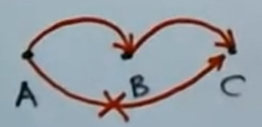
\includegraphics[scale=1]{Phil120Pictures/image1.png}\\
So the system in not transitive\\

\begin{tabular}{ccccc}
    $p$ & $q$ & $R(p,q)$ & $p\to q$ & $p\leftrightarrow q$\\
    \hline
    T & T & T & T & T\\
    T & F & T & F & F\\
    F & T & T & T & F\\
    F & F & T & T & T\\
    T & T & F & F & F\\
    T & F & F & F & F\\
    F & T & F & F & F\\
    F & F & F & F & F
\end{tabular}\\
\begin{tabular}{ccc}
    $p$ & $R(p,p)$ & $\lnot p$\\
    \hline
    T & T & F\\
    F & T & T
\end{tabular}\\
\begin{tabular}{ccccc}
    $p$ & $q$ & $R(p,q)$ & $p\wedge q$ & $p\vee q$\\
    \hline
    T & T & T & T & T\\
    T & F & T & F & T\\
    F & T & T & F & T\\
    F & F & T & F & F\\
    T & T & F & T & F\\
    T & F & F & F & F\\
    F & T & F & F & F\\
    F & F & F & F & F
\end{tabular}\\
Ex: $A$=``Plato was a student of Socrates"\\
$B$=``Aristotle was a student of Plato"\\
$C$=``Aristotle was a great logician"\\
Is $\lnot B\to(A\vee \lnot C)$ true or false?\\
$R(A,B)$, $R(B,C)$, $\sim R(A,C)$\\
Topics in $\lnot C$ are the same as topics in $C$ so we have $\sim R(A,\lnot C)$\\
So $A\vee \lnot C$ is F\\
Topics in $A\vee \lnot C$: topics in $A$ + topics in $\lnot C$ = \{Plato, students, Socrates, Aristotle, logician\}\\
$R(\lnot B,(A\vee\lnot C))$ is true\\
We have $\lnot B$ is F and $A\vee\lnot C$ is F so $\lnot B\to(A\vee\lnot C)$ is T\\

Ex2: Is the formula $(p\to q)\to(\lnot p\vee q)$ a tautology, contingency, or contradiction?\\
This would be done with a truth table\\

Ex3:\\
\argument{4}{$A\to C$\\
$B\to D$\\
$\lnot C\vee\lnot D$\\
\hline
$\therefore \lnot A\vee \lnot B$
}\\
$A\to C$ is T so $R(A,C)$ is T\\
$B\to D$ is T so $R(B,D)$ is T\\
$\lnot C\vee \lnot D$ is T so $R(C,D)$ is T\\
but $R(A,B)$ is F so $\lnot A\vee\lnot B$ is F\\

Aristotle's problem of future contingents:\\
Ex: ``Athens will win the sea battle tomorrow"\\
We can analyze cases like this using Lucasiewicz's Logic\\
This introduces a third truth value, I, meaning indeterminate/unknown\\
Analyzing these cases,\\
\begin{tabular}{cc|cccc}
    $p$ & $q$ & $p\& q$ & $p\vee q$ & $p\supset q$ & $p\equiv q$\\
    \hline
    T & I & I & T & I & I\\
    F & I & F & I & T & I\\
    I & T & I & T & T & I\\
    I & F & F & I & I & I\\
    I & I & I & I & T & T
\end{tabular}\\

Bochvor's System:\\
This deals with paradoxical systems and any operation involving and I will result in I.

\subsubsection{Term Logic}

Subject + Predicate\\
Ex: Victoria is the capital of BC\\
Victoria is the subject and ``is the capital of BC" is the predicate\\
This refers to a single individual object\\
Called \textit{singular sentence}\\

Ex2: Dogs are nice (creatures)\\
refers to a class/group/category//
called \textit{categorical sentence}\\
Def: A categorical sentence is one in which both subject and predicate are classes/sets/categories of objects that states an inclusion (or exclusion) relation between these two classes.\\

Term logic:\\
Capital letters stand for a description of a set/group of objects (with some property)\\
Ex: P=``UBC students", Q=``Dogs that like to chase cats", R=``Nice creatures"\\

Ex: All dogs are mammals\\
dogs are the subject and ``are" is called the \textit{copula}. Mammals is the predicate class.\\
This is \textit{total inclusion} (dogs is a subset of mammals)
Ex2: No dogs are cats\\
This is \textit{total exclusion} (the two sets have no overlap)\\
Ex3: Some dogs are US presidents\\
dogs is the subject, US presidents is the predicate class.\\
Some is defined as ``There exists at least one"\\
This is \textit{partial inclusion} (at least one object belongs to both sets)\\
Ex4: Some dogs are not UBC students\\
This is \textit{partial exclusion} (at least one object does not belong to both sets)\\

Types of claims:
\begin{itemize}
\item A: All $S$ are $P$ (universal affirmative)\\
If you're in $S$ then you're in $P$. ($p\supset q)$
\item E: No $S$ are $P$ (universal negative)\\
If you're in $S$ then you're not in $P$ ($p\supset\sim q$)
\item I: Some $S$ are $P$ (particular affirmative)\\
There exists at least one $S$ which is also in $P$
\item O: Some $S$ are not $P$ (particular negative)
\end{itemize}
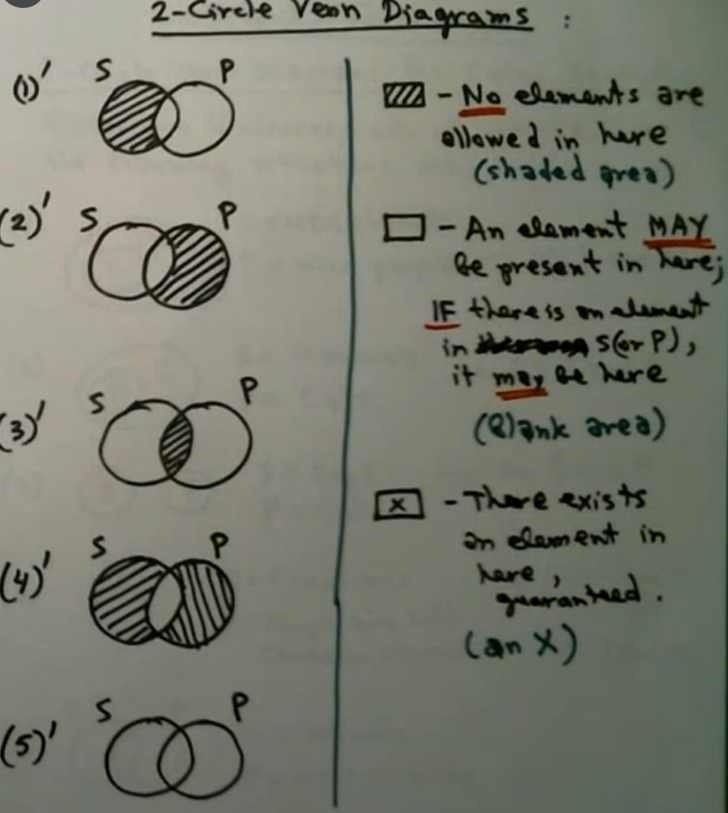
\includegraphics[scale=0.8]{Phil120Pictures/image2.png}\\

Def: The \textit{converse} of a categorical proposition is obtained by interchanging the proposition's subject and predicate terms\\
E and I types have their converse equal to their original claims but this is not the case for A and O claims.\\

Immediate inference:\\
Ex:\\
\argument{6}{No senators are politicians\\
\hline
No politicians are senators} (valid, E-conversion)\\
\argument{6}{Some books are valuable objects\\
\hline Some valuable objects are books} (valid, I-conversion)\\
\argument{6}{All students are hard workers\\
\hline
All hard workers are students} (invalid, A-conversion)\\
\argument{6}{Some mammals are not dogs\\
\hline
Some dogs are not mammals} (invalid, O-conversion)\\

The \textit{contrapositive} of a categorical proposition is obtained by converting it and negating both of its two non-logical terms\\
A and O types have their contrapositives equal to their original claims but E and I claims do not.\\

Ex:\\
\argument{7}{All men are mortal creatures\\
\hline All non-mortal creatures are non-men} (valid, A-contraposition)\\
\argument{7}{Some people are not bankers\\
\hline Some non-bankers are not non-people} (valid, O-contraposition)\\
\argument{7}{No students are employees\\
\hline No non-employees are non-students} (invalid, E-contrapostion)\\
\argument{7}{Some objects are red things\\
\hline Some non-red things are non-objects} (invalid, I-contraposition)\\

The \textit{obverse} of a categorical proposition is obtained by negating the predicate term and changing the proposition from affirmative to negative or from negative to affirmative.\\
i.e. All $S$ are $P$ $\to$ No $S$ are non-$P$\\
Some $S$ are $P$ $\to$ Some $S$ are not non-$P$\\
All A,E,I,O propositions are logically equivalent to their obverses\\

Contradiction\\
Given two contradictory propositions, at most one can be true and at most one can be false\\

Contrariety\\
Given two contrary propositions, at most one can be true, although both may be false\\

Subcontrariety\\
Given two subcontrary propositions, at most once can be false although both may be true\\

Ex: Contradiction\\
All human differences are determined by the environment\\
Not all human differences are determined by the environment\\

Ex: Contrariety\\
All human differences are determined by the environment\\
No human differences are determined by the environment\\

Ex: Subcontrariety\\
Some human differences are determined by the environment\\
Some human differences are not determined by the environment\\

Square of opposition:\\
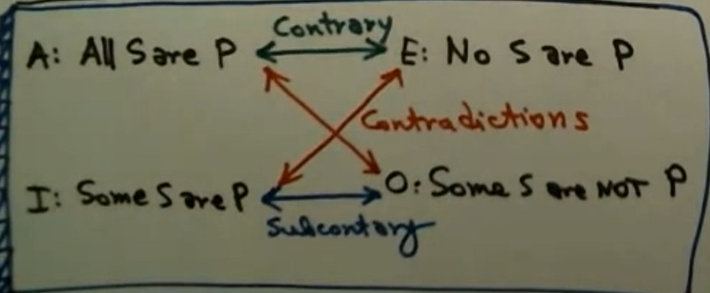
\includegraphics[scale=0.8]{Phil120Pictures/image3.png}\\
Ex: Not all people are cats\\
Not (all $S$ are $P$)\\
= Some $S$ are not $P$\\
Ex2: It's false that no people are students\\
Not (no $S$ are $P$)\\
= Some $S$ are $P$\\
Ex3: It's not true that all cats are not dogs\\
Not (no $S$ are $P$)\\
= Some $S$ are $P$\\

Syllogisms:\\
Def: A \textit{syllogism} is an argument in which there are exactly 3 non-logical referring terms, there are exactly 3 categorical propositions, and each term appears in exactly 2 of these propositions.\\
Ex:\\
\argument{6}{All whales are mammals\\
All mammals are nice\\
\hline All whales are nice}\\
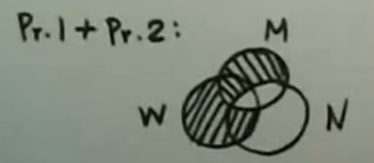
\includegraphics[scale=0.7]{Phil120Pictures/image4.png}\\

Ex2:\\
\argument{5}{All P are L\\Some G are P\\\hline Some G are L}\\
Def: the \textit{major term} appears in the predicate of the conclusion\\
The \textit{minor term} appears in the subject of the conclusion\\
The \textit{middle term} appears in both of the premises but not in the conclusion\\

Def: A referring term is \textit{distributed} iff that proposition says something about every member of that's term extension\\
A: All UBC students are people\\
So students would be distributed\\

In all universal claims (A,E) the subject is distributed\\
In all negative claims (E,O) the predicate is distributed\\

5 Rules for Validity of Syllogisms\\
All syllogisms must have the following:
\begin{itemize}
    \item A middle term that is distributed at least once
    \item Major and minor terms that are distributed in their premises if they are distributed in the conclusion
    \item At least one affirmative premise
    \item A negative conclusion iff one of the premises is negative\\
    i.e a) A negative conclusion and exactly one negative premise or\\
    b) An affirmative conclusion and either 2 premises are negative or none of the premises are negative\\
    The total number of negations must not be odd
    \item A particular premise if the conclusion is particular
\end{itemize}































































% Pre Calculus



\section{Pre-Calculus}

\subsection{Functions and Coordinates}

\subsubsection{Cartesian Coordinate System}
The Cartesian coordinate system is a graph to plot points, lines, and functions on a horizontal x-axis and vertical y-axis. The center where the lines meet is called the origin. The axes split the graph into 4 quadrants: QI, QII, QIII, QIV.\\
\centerline{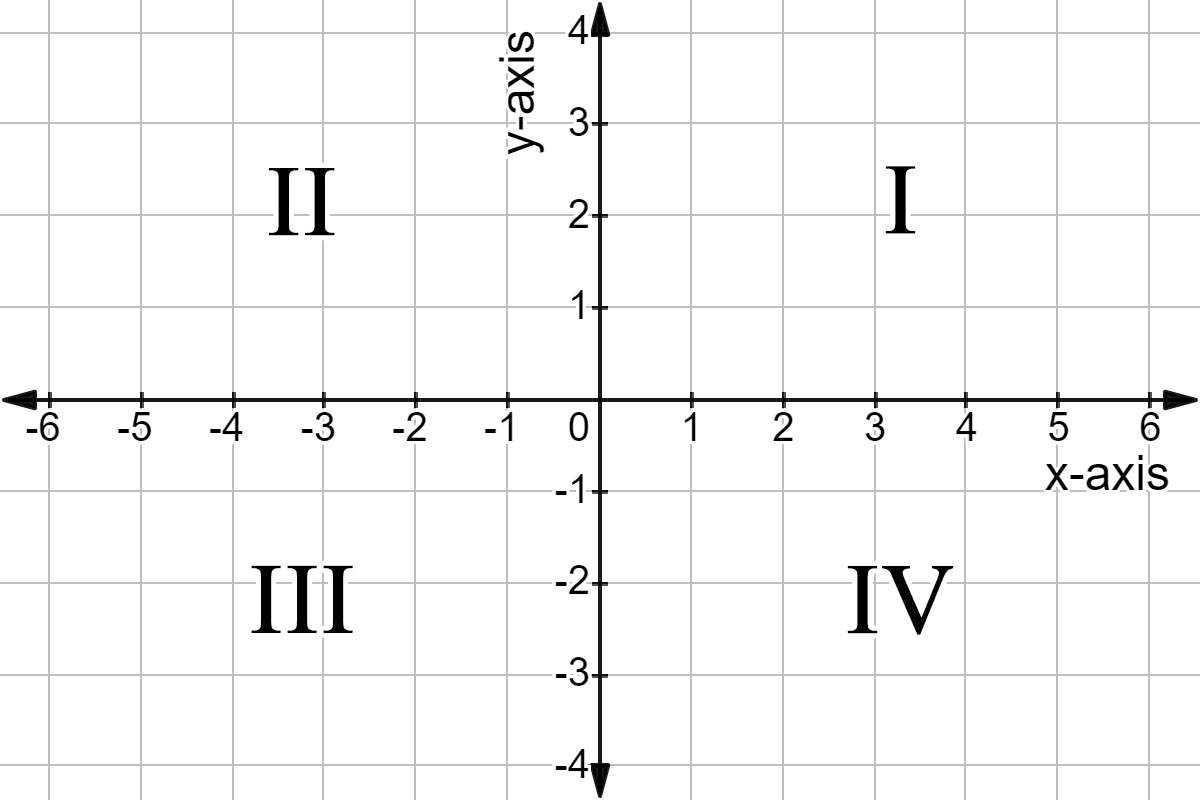
\includegraphics[scale =0.15]{PreCalcPictures/Cartesian Coordinate system.jpg}}
Points on the graph are denoted by $(x,y)$ and are called an ordered pair. Depending on if $x$ and $y$ are positive or negative, they will be positioned in different quadrants.\\
$(x,y)\rightarrow$QI\\
$(-x,y)\rightarrow$QII\\
$(-x,-y)\rightarrow$QIII\\
$(x,-y)\rightarrow$QIV\\
When graphing equations on the coordinate plane, the dependent variable will usually be on the x-axis and the independent variable will be displayed on the y-axis.

\subsubsection{Domain and Range}
Domain is the set of all elements that make up the x-coordinates.\\
Range is the set of all elements that make up the y-coordinates.\\
The domain and range can be expressed in multiple ways:
\begin{itemize}
    \item Inequality Description: $a<x<b$\\
    This means that x is greater than $a$ and less than $b$.
    \item Interval Notation: $x\in (a,b)$\\
    This means that $x$ is between $a$ and $b$, not including $a$ or $b$. If we use square brackets, $x\in [a,b]$, then it means $x$ is between $a$ and $b$ while including $a$ and $b$.\\
    Note that $\infty$ and $-\infty$ will always use round parentheses
    \item Set Notation: $\{x|a<x<b,x\in\mathbb{R}\}$\\
    This translates to the set of $x$ for which $x$ is greater than $a$ and less then $b$ for where $x$ is an element of all real numbers.
\end{itemize}

\subsubsection{Function Definition}
A function is a special type of relation where each element in the domain is associated with exactly one element in the range. (Every x-value can only have one associated y-value).\\
We can determine if a graph is a function or not using the vertical line test. If you move a vertical line along the graph, the line should intersect no more than one point on the curve.\\
Function notation, $f(x)$, is used to denote the result after some operation on the independent variable. $f(x)$ and $y$ are used somewhat interchangeably.










\subsection{Linear Functions}
A linear function is a function whose graph is a straight line. Its degree is 1 or 0. It has a constant rate of change.

\subsubsection{Slope}
Slope is a measure of how one quantity changes with respect to another, sometimes called the rate of change. For graphs, it is determined by calculating the change in the y-values over the change in x-values and is denoted by $m$.
$$m=\frac{\Delta y}{\Delta x}=\frac{y_2-y_1}{x_2-x_1}$$
For example, a line with slope $\frac{3}{2}$ will go up 3 units for every 2 units it goes across.\\
- Horizontal lines will always have a slope of 0.\\
- Vertical lines have an undefined slope ($\frac{1}{0}$).\\
- Parallel lines will have the same slope: $m_\parallel=m$.\\
- Perpendicular lines will have a slope that is equal to the negative reciprocal of the other. ${m_\perp=-\dfrac{1}{m}}$

\subsubsection{Equations of Linear Functions}
\begin{itemize}
    \item Slope Intercept Form: $y=mx+b$\\
    where $m$ is the slope and $b$ is the y-intercept. Slope intercept form is ideal for graphing the function and is the most commonly used.
    \item Slope Point Form: $y-y_1=m(x-x_1)$\\
    where $(x_1,y_1)$ is some point on the line. This is useful for when you are given a point and the slope and are asked to find an equation.
    \item General Form: $Ax+By+C=0$\\
    where $A$ must be a whole number and $B$ and $C$ are both integers. This is helpful for finding x and y intercepts.
\end{itemize}
All three forms are interchangeable.\\
\\
\textbf{Solving Linear Equations}\\
Often we are interested in when the line crosses the x-axis. We can find this by setting $y=0$ and solving for $x$.\\
Ex: $y=6x+4$
\begin{align*}
    0=&6x+4\\
    -4=&6x\\
    x=&-\frac{2}{3}
\end{align*}

\subsubsection{Systems of Linear Equations}
A system of linear equations is composed of two linear equations and is often referred to as a linear system.\\
A system will have no solutions if the lines are parallel.\\
A system will have infinite solutions if the lines are identical.\\
Otherwise, the system will have one solution.\\
\\
Solving Graphically:\\
The solution of a linear system can be estimated by graphing both equations. The solution will be where the two lines intersect. This will give a point that satisfies both equations. To verify the solution, you can plug the point back in to the original equations.\\
\centerline{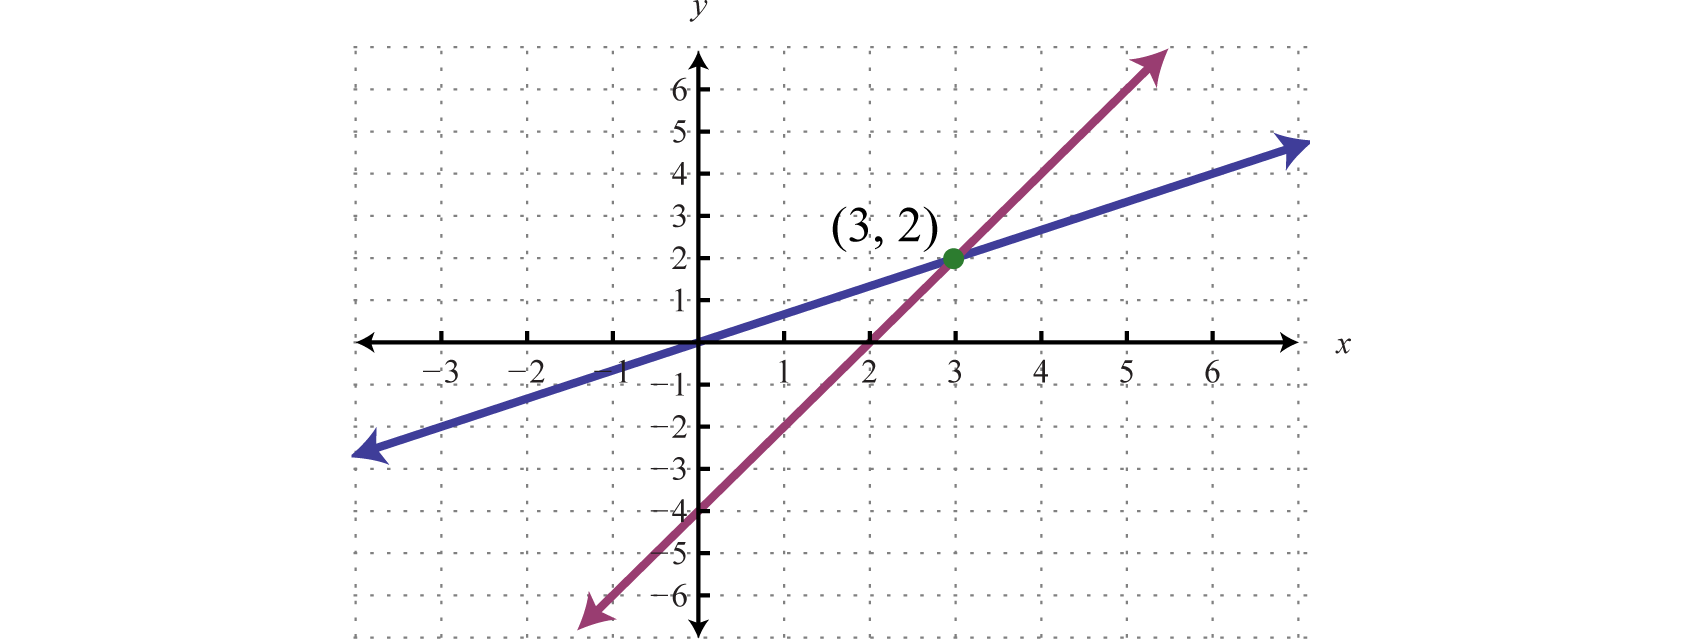
\includegraphics[scale=0.7]{PreCalcPictures/LinearSystemIntersection.png}}
Solving by Elimination\\
Step 1 is to make the value of $x$ or $y$ the same for both equations.\\
Step 2 is to add or subtract the add or subtract the equations to cancel out one of the variables.\\
Step 3 is to solve for the remaining variable.\\
Step 4 is to plug the value back into one of the original equations to solve for the other variable.\\
Ex: $\left\{\begin{matrix} 5x-3y=18\\
4x-6y=18 \end{matrix}\right.$
\begin{align*}
    &\left\{\begin{matrix}
    2(5x-3y=18)\\
    4x-6y=18
    \end{matrix}\right.\\
    &\left\{\begin{matrix}
    10x-6y=36\\
    4x-6y=18
    \end{matrix}\right.\\
    &(10x-6y)-(4x-6y)=36-18\\
    &6x=18\\
    &x=3\\
    &5(3)-3y=18\\
    &15-3y=18\\
    &-3y=3\\
    &y=-1\\
    &\mathrm{Solution}\,\mathrm{is}\,(3,-1)
\end{align*}
Solving by Substitution:\\
Step 1 is to isolate one of the variables in one equation.\\
Step 2 is, in the other equation, replace the variable you isolated for earlier with the equation that it's in terms of.\\
Step 3 is to solve for the remaining variable.\\
Step 4 is to plug the value bck into one of the original equations to solve for the other variable.\\
Ex: $\left\{\begin{matrix} x-3y=12\\
4x+2y=8 \end{matrix}\right.$
\begin{align*}
    & x=3y+12\\
    &4(3y+12)+2y=8\\
    &48+12y+2y=8\\
    &14y=-40\\
    &y=-\frac{20}{7}\\
    &x-3\left(-\frac{20}{7}\right)=12\\
    &x+\frac{60}{7}=\frac{84}{7}\\
    &x=\frac{24}{7}\\
    &\mathrm{Solution}\,\mathrm{is}\,\left(\frac{24}{7},-\frac{20}{7}\right)
\end{align*}

\subsubsection{Linear Inequalities}
Inequalities are in the form of $y\geq f(x)$. It creates a boundary, splitting the Cartesian plane into two or more regions. For $y\geq f(x)$, any part above the function is shaded and for $y\leq f(x)$, any part below the function is shaded. If $\geq$ or $\leq$ are used, the boundary will have a solid line. If $>$ or $<$ are used, the boundary will have dashed line.\\
\centerline{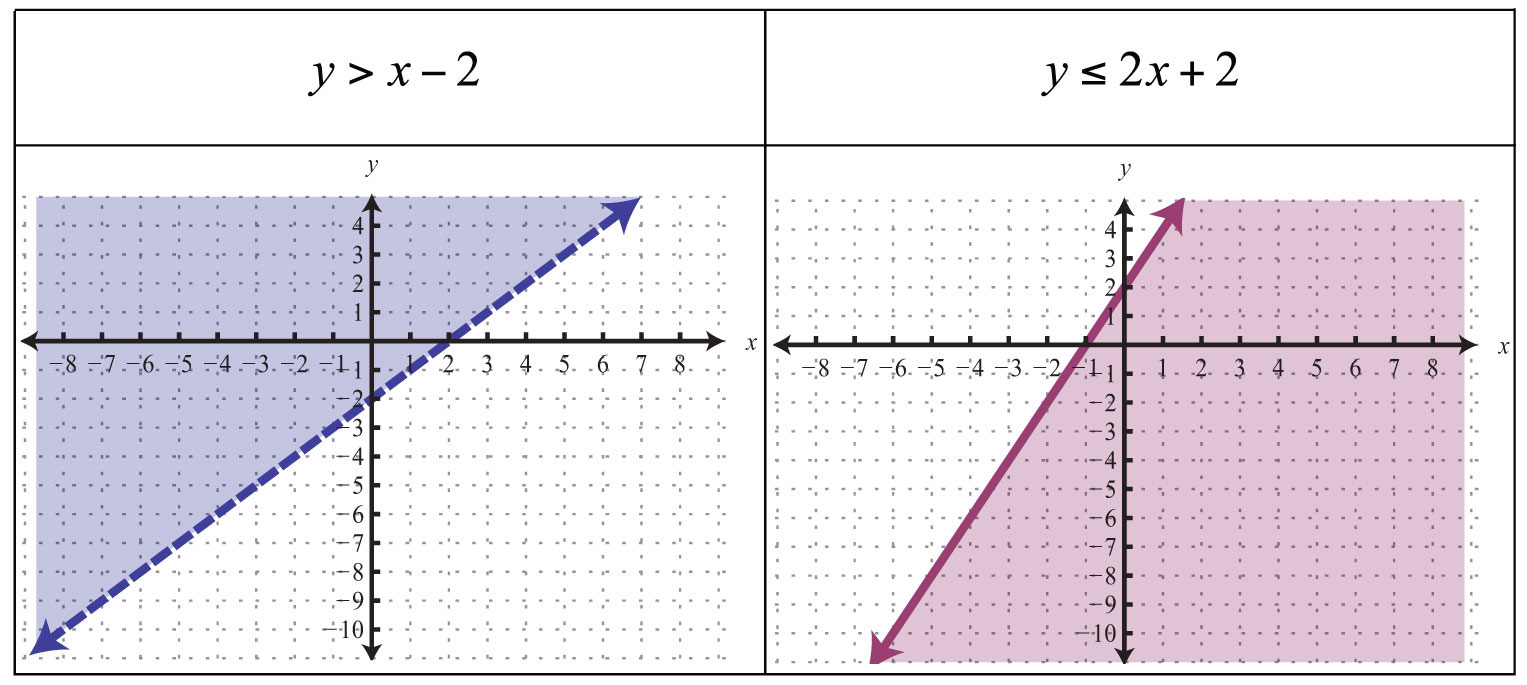
\includegraphics[scale = 0.3]{PreCalcPictures/LinearInequalities.jpg}}








\subsection{Quadratic Functions}
Quadratic functions are those in the form of $y=x^2$. They have a degree of 2. The shape of the graph is known as a parabola.

\subsubsection{Equations and Terminology}
Terminology:\\
The vertex is the lowest or highest point of the parabola (where it changes directions.)\\
The axis of symmetry is the vertical line that divides the parabola in half, going through the vertex.\\
A parabola will always have 1 y-intercept and either 0, 1, or 2 x-intercepts.\\
The domain of a parabola is $x\in\mathbb{R}$\\
The range of a parabola is dependent on which way it opens and the height of the vertex.\\
\\
\centerline{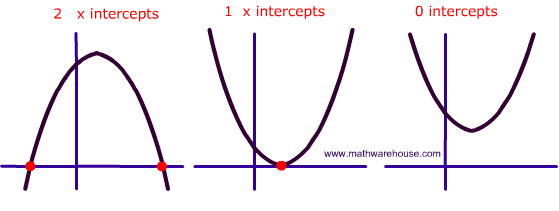
\includegraphics[scale = 0.6]{PreCalcPictures/ParabolaSolutions.png}}

Vertex Form: $y=a(x-p)^2+q$\\
$a$ determines how steep the parabola is. Larger values make it steeper and smaller values make it rise more gradually. If $a$ is positive, the parabola opens up. If $a$ is negative, the parabola opens down. $p$ determines how far to the right of the origin the vertex will be located. $q$ determines how far above the origin the vertex will be located.\\
This form is useful for graphing because you know exactly where the vertex is and how fast the slope is rising.\\
\\
Standard Form: $y=ax^2+bx+c$\\
$a$ determines how steep the parabola is and which way it opens. $c$ is the y-intercept.\\
This form is useful for solving quadratic equations.\\
\\
Converting between forms:\\
To convert vertex form to standard form, you simply need to expand the squared term inside the brackets.\\
To convert from standard form to vertex form, you can either use the conversion formulas of $p=-\dfrac{b}{2a}$ and $q=c-\dfrac{b^2}{4a}=c-ap^2$ or you can use completing the square method. Completing the square involves adding and subtracting a value in order to create a perfect square trinomial.\\
Ex: $x^2+6x+5$
\begin{align*}
    &x^2+6x+5+9-9\\
    &(x^2+6x+9)-4\\
    &(x+3)^2-4
\end{align*}
Ex2: $4x^2-32x-23$
\begin{align*}
    &4(x^2-8x)-23\\
    &4(x^2-8x+16)-23-4(16)\\
    &4(x^2-4)^2-87
\end{align*}

\subsubsection{Solving Quadratic Equations}
Solving by Factoring:
First we must set $y=0$. Then we can factor our quadratic. We will have two terms. At least one of the terms must be equal to zero in order to give an answer of zero so to solve, we can set both terms equal to zero and solve for $x$.\\
Ex: $y=x^2+4x-21$
\begin{align*}
    0=&(x+7)(x-3)\\
    0=&(x+7)\Ra x=-7\\
    0=&(x-3)\Ra x=3
\end{align*}
\\
Solving by Completing the Square:\\
Ex: $y=x^2-6x+7$
\begin{align*}
    y=&x^2-6x+9+7-9\\
    y=&(x-3)^2-2\\
    0=&(x-3)^2-2\\
    2=&(x-3)^2\\
    x-3=&\pm \sqrt{2}\\
    x=&3\pm \sqrt{2}
\end{align*}
\\
The Quadratic Formula:\\
Derivation:\\
If there is no horizontal shift, a quadratic will take the form $y=ax^2+q$ and solving the quadratic is easy. We can make any quadratic take this form by applying a horizontal translation, shifting the quadratic by the location of the vertex. So we set $x=x_s-\frac{b}{2a}$. This will allow us to solve for any quadratic.
\begin{align*}
    0=&ax^2+bx+c\\
    0=&a\left(x_s-\frac{b}{2s}\right)^2+b\left(x_s-\frac{b}{2a}\right)+c\\
    0=&\left(x_s-\frac{b}{2s}\right)^2+\frac{b}{a}\left(x_s-\frac{b}{2a}\right)+\frac{c}{a}\\
    0=&x_s^2-\frac{b}{a}x_s+\frac{b^2}{4a^2}+\frac{b}{a}x_s+\frac{c}{a}\\
    x_s^2=&\frac{b^2}{4a^2}-\frac{c}{a}=\frac{b^2-4ac}{4a^2}\\
    x_s=&\pm\frac{\sqrt{b^2-4ac}}{2a}\\
    x=&x_s-\frac{b}{2a}=-\frac{b}{2a}\pm\frac{\sqrt{b^2-4ac}}{2a}\\
    x=&\frac{-b\pm\sqrt{b^2-4ac}}{2a}
\end{align*}
*A similar derivation could be done using the complete the square method.\\
This formula allows us to solve any quadratic equation. It also has a property that allows us to deduce how many solutions a quadratic will have without actually solving it. This is done using the discriminant (the part under the square root).\\
If $b^2-4ac>0$ there are 2 real solutions\\
If $b^2-4ac=0$ there is 1 real solution\\
If $b^2-4ac<0$ there are no real solutions\\
\\
Systems of Quadratic Equations:\\
To find the point(s) where two quadratics intersect, we can use substitution for $y$ and set the two equations equal to each other. This gives a new quadratic and will give the points of intersection.\\
Ex: $\left\{\begin{matrix} y=3x^2-x-2\\
y=6x^2+4x-4 \end{matrix}\right.$
\begin{align*}
    3x^2-x-2=&6x^2+4x-4\\
    0=&3x^2+5x-2\\
    0=&(3x-1)(x+2)\\
    0=&(3x-1)\Ra x=\frac{1}{3}\\
    0=&(x+2)\Ra x=-2
\end{align*}

\subsubsection{Quadratic Inequalities}
Because a quadratic can have two x-intercepts, it can have two places it switches from positive to negative so quadratic inequalities are often bounded by two numbers.\\
We can break it up into a series of linear cases based on factors.\\
Ex: $(x+3)(x-2)\geq 0$\\
$x+3\geq 0\Ra x\geq -3$\\
\centerline{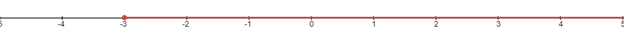
\includegraphics[]{PreCalcPictures/Inequality1.png}}
$x-2\geq 0\Ra x\geq 2$\\
\centerline{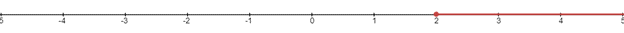
\includegraphics[]{PreCalcPictures/Inequality2.png}}
$(x+3)(x-2)\geq 0\Ra x\leq -3\,\mathrm{or}\,x\geq 2$\\
\centerline{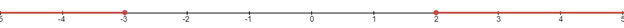
\includegraphics[]{PreCalcPictures/Inequality3.png}}
This method of lining up the number line graphs works for all polynomials and even rational expressions to solve for difficult inequalities.








\subsection{Transforming Functions}

\subsubsection{Transformations}
Transformations are when the graph of a relation is shifted or changed. An image point is the point that results from a transformation. Mapping relates one set of points to the corresponding points in the image.\\
\\
Vertical translations move the graph up or down, specified by the value $k$.
$$f(x)\rightarrow f(x)+k$$
Mapping notation: $(x,y)\rightarrow(x,y+k)$\\
\\
Horizontal translations move the graph left or right specified by the value $h$.
$$f(x)\rightarrow f(x-h)$$
Mapping notation: $(x,y)\rightarrow(x-h,y)$\\
\\
Reflections across the x-axis:
$$f(x)\rightarrow -f(x)$$
Mapping notation: $(x,y)\rightarrow (x,-y)$\\
\\
Reflections across the y-axis:
$$f(x)\rightarrow f(-x)$$
Mapping notation: $(x,y)\rightarrow(-x,y)$\\
\\
Vertical stretches multiplies all y-coordinates by a factor of $a$.
$$f(x)\rightarrow af(x)$$
Mapping notation: $(x,y)\rightarrow (x,ay)$\\
\\
Horizontal stretches multiply all x-coordinates by a factor of $b$.
$$f(x)\rightarrow f\left(\frac{1}{b}x\right)$$
Mapping notation: $(x,y)\rightarrow(bx,y)$\\
\\
All together, we can use transformations to manipulate ordinary functions into various forms. The order transformations are applied is stretches and reflections are applied first and then translations after.
$$f(x)\rightarrow af\left(\frac{x}{b}-h\right)+k$$
Mapping notation: $(x,y)\rightarrow (bx-h,ay+k)$\\
Points that do not change given a series of transformations are called invariant points.

\subsubsection{Absolute Value of a Function}

Given the property of the absolute value, the function will have all y-values be positive with the negative values being reflected across the x-axis. The range of an absolute value function cannot contain negative values.
$$y=|f(x)|$$
Mapping notation: $(x,y)\rightarrow(x,|y|)$\\
Absolute value functions can be described in two different ways: The root of a square, $$|f(x)|=\sqrt{(f(x))^2}$$
or as a piecewise function:
$$|f(x)|=\left\{\begin{matrix} f(x)\,&\mathrm{if}\,f(x)\geq 0\\ -f(x)\,&\mathrm{if}\,f(x)<0\end{matrix}\right.$$
Piecewise functions are not limited to absolute value functions. They are functions comprised of multiple parts or functions over different domains.\\
\\
Solving Absolute Value Equations:\\
When solving for absolute value equations, we must consider both cases, $f(x)$ and $-f(x)$, and check our restrictions after.\\
Ex: $|2x-5|=5-3x$
\begin{align*}
    &\text{Case 1: } |2x-5|=2x-5\text{ for }x\geq\frac{5}{2}\\
    &2x-5=5-3x\\
    &5x=10\\
    &x=2\\
    &\text{Because }x\ngeq\frac{5}{2}\text{, the solution is extraneous.}\\
    &\text{Case 2: } |2x-5|=5-2x\text{ for }x<\frac{5}{2}\\
    &5-2x=5-3x\\
    &x=0\\
    &\text{Check }x<\frac{5}{2}\,\therefore\text{ it is a solution}
\end{align*}
Ex: $|x^2-2x|=-1$
\begin{align*}
    &\text{Case 1: }|x^2-2x|=x^2-2x\text{ for }x\leq 0\text{ or }x\geq 2\\
    &x^2-2x+1=0\\
    &(x-1)^2=0\\
    &x-1=0\\
    &x=1\\
    &\text{Check restrictions: }x=1\text{ is extraneous}\\
    &\text{Case 2: }|x^2-2x|=2x-x^2\text{ for }0<x<2\\
    &2x-x^2=-1\\
    &x^2-2x-1=0\\
    &x=\frac{2\pm\sqrt{8}}{2}=1\pm\sqrt{2}\\
    &\text{Check restrictions: both extraneous}\\
    &\therefore\text{ no real solutions}
\end{align*}
Absolute Value Inequalities:\\
$$|f(x)|<k\Ra-k<f(x)<k$$
\subsubsection{Reciprocal of a Function}
The reciprocal of a function introduced a few interesting new aspects.
$$y=\frac{1}{f(x)}$$
Mapping notation: $(x,y)\rightarrow (x,\frac{1}{y}$\\
The reciprocal will have vertical asymptotes where $f(x)=0$ in the original function and a horizontal asymptote at $y=0$. An asymptote is an imaginary line that the function comes infinitely close to but never reaches. The reciprocal will have invariant points any place where $y=1$ in the original function.\\
Ex: $y=\frac{1}{x^2-4}$\\
\centerline{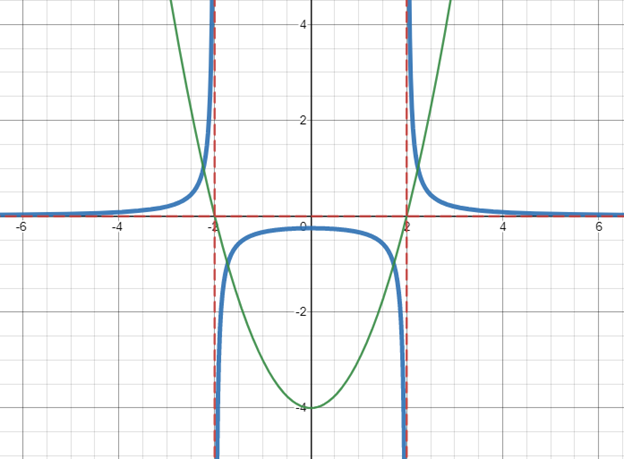
\includegraphics[scale = 0.5]{PreCalcPictures/ReciprocalEx.png}}

\subsubsection{Inverse Functions}
The inverse of a function reverses the process represented by that function, interchanging $x$ and $y$ coordinates. The result is a reflection along the line $y=x$. Inverse notation is $f^{-1}(x)$ or $x=f(y)$.\\
Mapping notation: $(x,y)\rightarrow(y,x)$\\
To solve for the inverse of a function, switch $x$ and $y$ and then solve for $y$.\\
Ex: Inverse of $y=\frac{1}{2x+5}$
\begin{align*}
    x=&\frac{1}{2y+5}\\
    x(2y+5)=&1\\
    2y+5=&\frac{1}{x}\\
    2y=&\frac{1}{x}-5\\
    y=&\frac{1}{2x}-\frac{5}{2}
\end{align*}
Ex2: Inverse of $y=x^2+2x-2$
\begin{align*}
    x=&y^2+2y-2\\
    x=&y^2+2y+1-2+1\\
    x=&(y+1)^2-1\\
    x+1=&(y+1)^2\\
    \pm\sqrt{x+1}=&y+1\\
    y=&\pm\sqrt{y+1}-1
\end{align*}
\subsubsection{Square Root of a Function}
A square root function is the inverse of a quadratic. Because the inverse of a parabola does not meet the requirements of a function, we can restrict the range in order to make it a function. In doing this, we state that the square root must always be positive and this goes for all functions.
$$y=\sqrt{f(x)}$$
Mapping notation: $(x,y)\rightarrow(x,\sqrt{y})$\\
The square root of a function will travel in the same direction as the original function but the shape and value will be different.
For $f(x)<0$, $\sqrt{f(x)}$ is undefined\\
For $0<f(x)<1$, $\sqrt{f(x)}>f(x)$\\
For $f(x)>1$, $\sqrt{f(x)}<f(x)$\\
Note that we must restrict the domain of $x$ such that the value of $f(x)>0$\\
An interesting thing to note is that the square root of any downward opening parabola forms a semicircle.\\
\\
Solving radical equations:\\
Ex: $\sqrt{x-2}=4-x$
\begin{align*}
    &\text{Restrictions: }x-2\geq 0\Ra x\geq 2\\
    &\text{and }x-4\geq 0\Ra x\leq 4\\
    &(\sqrt{x-2})^2=(4-x)^2\\
    &x-2=16-8x+x^2\\
    &x^2-9x+18=0\\
    &(x-3)(x-6)=0\\
    &x=3,x=6\\
    &x=6\nleq 4\,\therefore \text{ not a solution}\\
    &\Ra x=3
\end{align*}
\subsubsection{Rational Functions}
Rational functions are an algebraic fraction with a numerator and denominator that are polynomials. In other words, it is a function divided by a function.\\
Ex: $\dfrac{x-7}{x^2-4x+3}$\\
\\
The graphs of rational functions can have a variety of features including asymptotes and holes. Asymptotes and holes occur at points where the function is not defined (divided by 0). These values for which the denominator is equal to 0 are called non-permissible value (NPVs).\\
Ex: NPVs of $\dfrac{x-7}{(x-3)(x-1)}$ are $x\neq3$ and $x\neq 1$\\
\\
Solving Rational Functions:\\
The x-intercepts of a rational function occur where the numerator is equal to 0 (given the denominator is not also 0).\\
Ex: $\dfrac{6-x}{2x}\Ra6-x=\Ra x=6$\\
\\
Simplifying Rational Expressions:\\
Some rational expressions can be factored and simplified.\\
Ex: $\dfrac{6-2x}{x^2-9}=\dfrac{-2(x-3)}{(x+3)(x-3)}$\\
The $(x-3)$ terms cancel, leaving $\dfrac{-2}{x+3}$.\\
Note that you must include all original NPVs. Otherwise, the simplified function would not be the same as the original. This new, simplified function will have a hole (removable discontinuity) at the point $x=3$, the term that was removed.\\
So, our final answer is $\dfrac{-2}{x+3}$ where $x\neq\pm3$\\
\\
Operations with Rational Expressions:\\
When dividing two rational expressions, we must take the NPVs of both expressions at the start and then once more after dividing.\\
Ex: $\dfrac{3x^2}{y^2}\div\dfrac{x}{y}\to$ NPVs: $y\neq0$\\
$\dfrac{3x^2y}{xy^2}\to$ NPVs: $y\neq0,\,x\neq0$\\
When adding and subtracting rational epressions, you must find the LCM and multiply the expressions accordingly as you do with regular addition and subtraction with fractions.\\
Ex: $\dfrac{5x}{x+2}+\dfrac{2x-3}{x-1}=\dfrac{5x(x-1)+(2x-3)(x+2)}{(x+2)(x-1)}$ where $x\neq-2,\,x\neq1$\\
\\
Asymptotes:\\
Vertical asymptotes occur at points where the function has NVPs that are not holes. For example, $\frac{1}{x}$ has a vertical asymptote at $x=0$. At these asymptotes, the function will curl up or down towards $y=\infty$ or $y=-\infty$.\\
Horizontal asymptotes are the end behavior of rational functions. As $x$ approaches positive or negative infinity, the function will either diverge (go to infinity) or approach a finite value as a horizontal asymptote.
\begin{itemize}
    \item If the degree of the numerator is greater than the degree of the denominator, $f(x)\to\pm\infty$
    \item If the degree of the numerator is the same as the degree of the denominator, $f(x)\to L$ where $L$ is some constant.
    \item If the degree of the numerator is less than the degree of the denominator, $f(x)\to 0$
\end{itemize}









\subsection{Conic Sections}
Conic sections include four distinct shapes: circles, ellipses, parabolas, and hyperbolas. They are called conic sections because they can be formed from cutting a cone in different ways.\\
\centerline{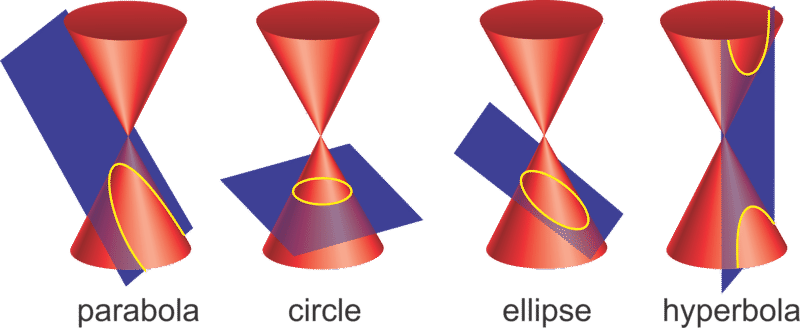
\includegraphics[scale=0.5]{PreCalcPictures/ConicSections.png}}

\subsubsection{Circles}
The standard equation for a circle is $(x+h)^2+(y-k)^2=r^2$ where the point $(h,k)$ is where the center of the circle is located and $r$ is the radius of the circle.\\
If given the equation of a circle in expanded form, you can complete the square for both $x$ and $y$ to change it to standard form.\\
\begin{align*}
    \text{Ex: } &x^2-2x+y^2+4y-4=0\\
    &(x^2+2x+1)+(y^2+4y+4)-4=1+4\\
    &(x-1)^2+(y+2)^2=9
\end{align*}

\subsubsection{Ellipses}
An ellipse is a circular object with two radii of different length.\\
Terminology:
\begin{itemize}
    \item The major axis is the longer axis (twice the length of the longer radius)
    \item The minor axis is the shorter axis (twice the length of the shorter radius)
    \item The vertices are the two points on either end of the major axis
    \item The co-vertices are the two points on either end of the minor axis
    \item The foci of an ellipse are two whose sum of distances from any of point on the ellipse is always the same. They lie on the major axis and are equidistant away from the origin.
    \item The distance between each focus and the center is called the focal length $f$ where $f^2=p^2-q^2$ where $p$ is the major radius and $q$ is the minor radius.
\end{itemize}
The standard equation for an ellipse is $\dfrac{(x-h)^2}{a^2}+\dfrac{(y-k)^2}{b^2}=1$ where t $(h,k)$ is the center point, $a$ is the horizontal axis, $b$ is the vertical radius.

\subsubsection{Parabolas}
Parabolas can be viewed as the set of all points whose distance from a certain point (the focus) is equal to their distance from a certain line called the directrix. The focus (point $(a,b)$) will always be the same distance away from the directrix (line $y=k$) along the curve of the parabola.\\
\centerline{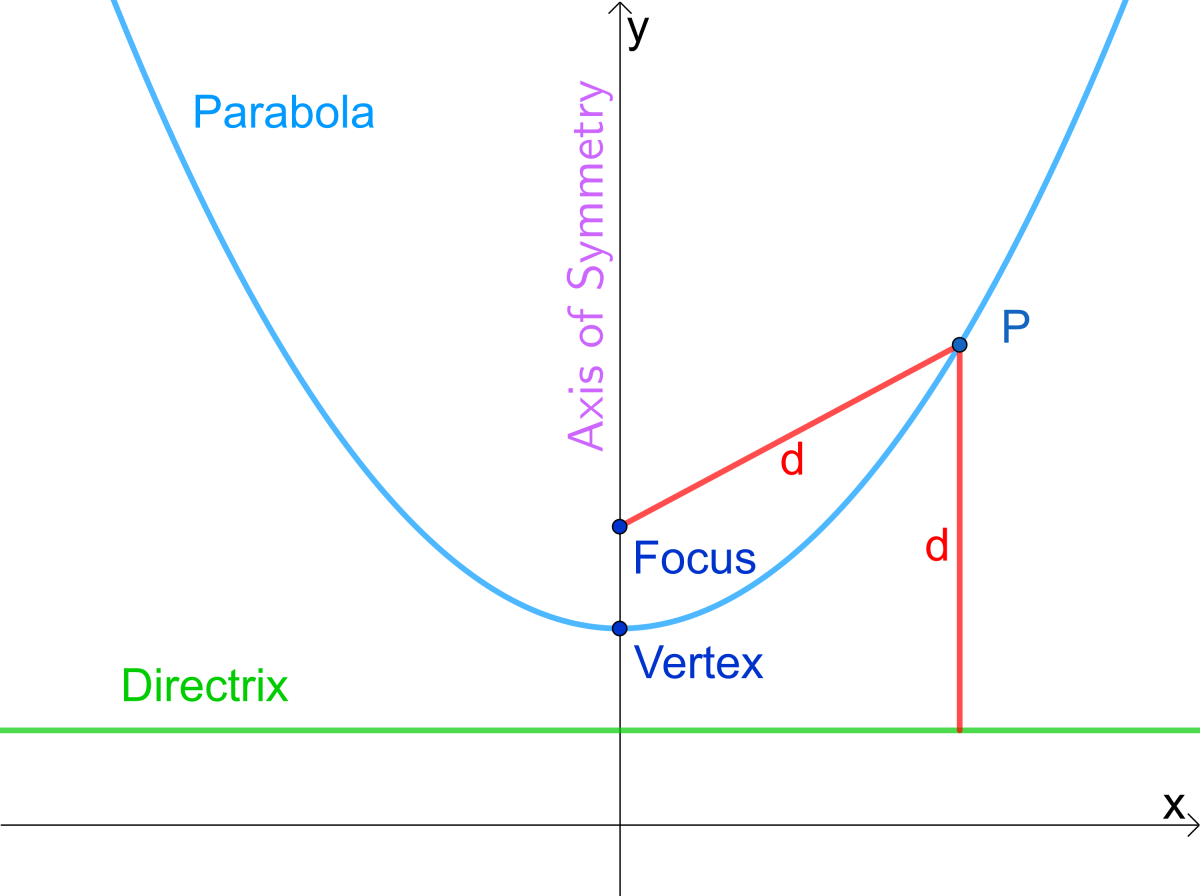
\includegraphics[scale=1.2]{PreCalcPictures/ParabolaConic.png}}
The equation of a parabola can be derived from the location of the focus and directrix using the equation $y=\dfrac{(x-a)^2}{2(b-k)}+\dfrac{b+k}{2}$\\
The location of the focus and directrix can be found from the equation of a quadratic by working backwards with the same formula.\\
Ex: $y=2(x-1)^2+4\Ra a=1$\\
\begin{align*}
    &2=\frac{1}{2(b-k)} &4=\frac{b+k}{2}\\
    &b-k=\frac{1}{4} &b=8-k\\
    &\frac{1}{4}=8-2k &\\
    &k=\frac{31}{8}\\
    &8-\frac{31}{8}=b\\
    &b=\frac{33}{8}
\end{align*}

\subsubsection{Hyperbolas}
There are two cases of hyperbolas defined by two slightly different equations: $\dfrac{(x-h)^2}{a^2}-\dfrac{(y-k)^2}{b^2}=1$ or $\dfrac{(y-k)^2}{b^2}-\dfrac{(x-h)^2}{a^2}=1$\\
If the x-term is positive, the hyperbola will open up to the side. if the y-term is positive, the hyperbola will open up.\\
$a$ is always associated with the x-term and $b$ is always associated with the y-term.\\
The point $(h,k)$ will be the center of the hyperbolas and the point $a$ or $b$ determines how far away the vertices of the hyperbola will be from its center. Each hyperbola will have 2 diagonal asymptotes that meet in its center. The slopes of the asymptotes will always be $m_{asym}=\pm\frac{b}{a}$\\
\centerline{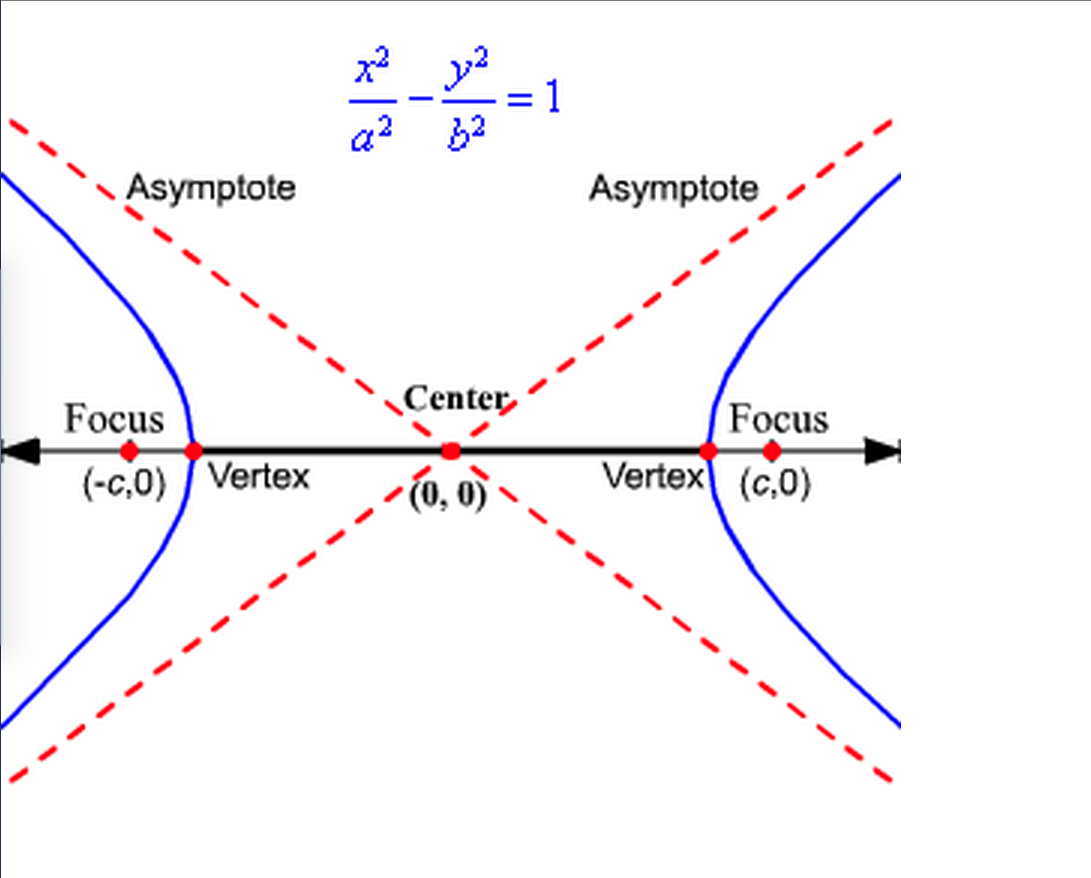
\includegraphics[scale=0.3]{PreCalcPictures/HyperbolaGraph.png}}
The difference from each focus to a point on the hyperbola will always be a constant $|d_1-d_2|=C$. If it opens horizontally, it will be $|d_1-d_2|=2a$ and if it opens vertically, it will be $|d_1-d_2|=2b$. The distance from each focus to the center of the hyperbola is $f^2=a^2+b^2$.








\subsection{Polynomial Functions}

\subsubsection{Polynomials}
A polynomial function is a function in the form of $f(x)=a_nx^n+a_{n-1}x^{n-1}+\cdots+a_1x+a_0$\\
Definitions: degree of a polynomial is the highest exponent of $x$ in the function. End behavior is the y-values as $|x|$ gets increasingly large.\\ Even/odd polynomials refers to the highest degree. Even polynomials will always start and end in the same direction (as in start above the x-axis and end above the x-axis). Odd polynomials will keep the same path and will always cross over the x-axis, ensuring that they will always have at least one solution.
\subsubsection{Polynomial Division}
Any polynomial divided by another polynomial to get a quotient and a remainder.\\
Long Division Method:\\
The goal is to elliminate the head term each time/ To do this, multiply the polynomial by a LCM and write what we had to multiply it by in each case above.\\
Ex: $\dfrac{6x^3-2x^2+x+3}{x^2-x+1}$\\
\polylongdiv[style=A]{6x^3-2x^2+x+3}{x^2-x+1}\\
$\dfrac{6x^3-2x^2+x+3}{x^2-x+1}=6x+4+\dfrac{x-1}{x^2-x+1}$\\
\\
Synthetic Division Method:\\
We set it up taking the coefficients of each x-term in the top row of the box and the solution of the binomial on the outside.\\
We bring the first number down and then multiply it by $3$ and bring it up.\\
Then we take the $15$ and add it with the $-12$ and bring the sum to the bottom. The process is repeated and the coefficients on the bottom will form the answer as well as the remainder.\\
Ex: $\dfrac{4x^3+15x^2+7x-10}{x+3}$\\
 \polyhornerscheme[x=-3]{4x^3+15x^2+7x-10}\\
 $\dfrac{4x^3+15x^2+7x-10}{x+3}=4x^2+3x-2-\dfrac{4}{x+3}$
 
\subsubsection{Factoring Polynomials}
Remainder Theorem:\\
When a polynomial, $P(x)$, is divided by a binomial of the form $x-a$, the remainder is $P(a)$. A polynomial divided by one of its factors will have no remainder. So $P(a)=0$ for where $a$ is a solution.\\
Factor Theorem:\\
$x-a$ is a factor of $P(x)$ if and only if $P(a)=0$.\\
Integral Zero Theorem:\\
If $x-a$ is a factor of $P(x)$, $a$ is a factor of the constant term.\\
Ex: possible factors of $x^2+2x-10$ could include $a$ values of $\{\pm1,\pm2,\pm5,\pm10\}$.\\
When there is a coefficient in front of the leading term, you must take factors of the constant term divided by the coefficient.\\
Ex: Possible $a$-values of $4x^3+39x^2+54x-16$:\\
Factors of $-16$: $\{\pm1,\pm2,\pm4,\pm8,\pm16\}$\\
Factors of $4$: $\{\pm1,\pm2,\pm4\}$\\
$\dfrac{\text{Factors of }-16}{\text{Factors of }4}:\,\{\pm1,\pm\frac{1}{4},\pm\frac{1}{2},\pm2,\pm4,\pm8,\pm16\}$\\
By using the remainder theorem and polynomial division, we can fully factor any degree polynomial.\\
Ex: Factor $x^4+4x^3-10x^2-28x-15$\\
\begin{align*}
    &\text{Factors of }-15:\,\{\pm1,\pm3,\pm5,\pm15\}\\
    &P(-1)=(-1)^4+4(-1)^3-10(-1)^2-28(-1)-15=0\therefore x+1\text{ is a factor}
\end{align*}
\polyhornerscheme[x=-1]{x^4+4x^3-10x^2-28x-15}
\begin{align*}
    &x^4+4x^3-10x^2-28x-15=(x+1)(x^3+3x^2-13x-15)\\
    &\text{Factors of }-15:\,\{\pm1,\pm3,\pm5,\pm15\}\\
    &P(3)=(3)^3+3(3)^2-13(3)-15=0\therefore x-3\text{ is a factor}
\end{align*}
\polyhornerscheme[x=3]{x^3+3x^2-13x-15}
\begin{align*}
    &x^4+4x^3-10x^2-28x-15=(x+1)(x-3)(x^2+6x+5)\\
    &=(x+1)(x-3)(x+5)(x+1)\\
    &=(x+5)(x-3)(x+1)^2\\
    &x=-5,-1,3
\end{align*}

\subsubsection{Graphs}
All polynomials are continuous functions.\\
Multiplicity refers to the number of times the zero of a function occurs.\\
Ex: $(x-1)^2$ has a multiplicity of 2.\\
When a function has an odd multiplicity, it crosses the x-axis. When it has an even multiplicity, it touches the x-axis and "bounces off", coming back in the same direction.\\
To graph a polynomial, first factor it and plot the zeros. Then look at the end behavior and the multiplicity. You can use calculus to find the locations of the peaks and valleys.








\subsection{Exponential and Logarithmic Functions}

\subsubsection{The Exponential Function}
Exponential functions are those in the form of $y=c^x$ for where $c\neq0$ and $c\neq 1$\\
The general form is:
$$f(x)=ac^{\frac{x-h}{b}}+k$$
If $c>1$, the graph will model exponential growth and tend to infinity.\\
If $0<c<1$, the graph will model exponential decay and will tend to 0.\\
\\
Solving same base equations:\\
Some exponential equations can be solved by setting the bases of both sides equal to another.\\
\begin{align*}
    \text{Ex: }&16^{x+3}=\left(\frac{1}{8}\right)^{x-10}\\
    &(2^4)^{x+3}=(2^{-3})^{x-10}\\
    &2^{4x+12}=2^{-3x+30}\\
    &4x+12=-3x+30\\
    &7x=18\\
    &x=\frac{18}{7}
\end{align*}

\subsubsection{Logarithms}
Logarithms are the inverse of exponentials.
\begin{align*}
    y=c^x\to x&=c^y\\
    \log_cx&=\log_c(c^y)\\
    \log_cx&=y\log_cc\\
    y&=\log_cx
\end{align*}
They have the restrictions that $c>0$, $c\neq 1$ and $x>0$\\
Notation:\\
$\log_{10}x=\log x$ and is called the common logarithm.\\
$\log_ex=\ln x$ and is called the natural logarithm.\\
\\
Log Rules:
\begin{align*}
    &\log_c1=0\\
    &\log_cc=1\\
    &c^{\log_cx}=x\\
    &\log_ca+\log_cb=\log(_c(ab)\\
    &\log_ca-\log_cb=\log\left(\frac{a}{b}\right)\\
    &\log_ca^n=n\log_ca\\
    &\log_cx=\frac{\log_nx}{\log_nc}\\
    &a^x=e^{x\ln a}
\end{align*}

\subsubsection{Solving Equations}
We can solve logarithmic and exponential equations using the log rules mentioned.
\begin{align*}
    \text{Ex: }&2^x=3^{x+1}\\
    &\log_3(2^x)=\log_3(3^{x+1})\\
    &x\log_32=x+1\\
    &x(\log_32-1)=1\\
    &x=\frac{1}{\log_32}
\end{align*}
\begin{align*}
    \text{Ex2: }&\log(x+2)+\log(x-1)=1\\
    &\text{Restrictions: }x+2>0\Ra x>-2\text{ and }x-1>0\Ra x>1\\
    &\log((x+2)(x-1))=1\\
    &\log((x+2)(x-1))=\log10\\
    &(x+2)(x-1)=10\\
    &x^2+x-2=10\\
    &x^2+x-12=0\\
    &(x+4)(x-3)=0\\
    &x=-4,\,x=3\\
    &-4\ngeq 1\therefore\,x=-4\text{ is extraneous}\\
    &\Ra x=3
\end{align*}
\begin{align*}
    \text{Ex3: }&2\log_2(x-1)=1-\log_2(x+2)\\
    &\text{Restrictions: }x-1>0\Ra x>1\text{ and }x+2>0\Ra x>-2\\
    &\log_2(x-1)^2=\log_22-\log_2(x+2)\\
    &\log_2(x-1)^2=\log_2\left(\frac{2}{x+2}\right)\\
    &(x-1)^2=\frac{2}{x+2}\\
    &(x^2-2x+1)(x+2)=2\\
    &x^3+2x^2-2x^2-4x+x+2=2\\
    &x^3-3x=0\\
    &x(x+\sqrt{3})(x-\sqrt{3})=0\\
    &x=0,\pm\sqrt{3}\\
    &\text{by restrictions, }x=\sqrt{3}
\end{align*}

\subsubsection{Applications}
Exponential growth/decay model:\\
$F=Ir^{\frac{t}{T}}$ where $F$ is the final amount, $I$ is the initial amount, $r$ is the rate of growth/decay per time interval $T$. $t$ is time.\\
Ex: A bacteria doubles every 4 hours. If there were 100 to start, when will there be 500,000?
\begin{align*}
    &500000=100(2)^{\frac{t}{4}}\\
    &5000=2^\frac{t}{4}\\
    &\log5000=\frac{t}{4}\log2\\
    &t=\frac{4\log5000}{\log2}\approx49.15\text{ hours}
\end{align*}
Compound growth model:\\
$A=I\left(1+\frac{r}{n}\right)^{nt}$ where $A$ is the final amount, $I$ is the initial amount, $r$ is the rate per year, $t$ is times, and $n$ is the number of compound periods per year.\\
Ex: $\$15000$ is invested at $5.5\%$ APR, compounded monthly. How long will it take to grow to $\$450000$?
\begin{align*}
    &450000=15000\left(1+\frac{0.055}{12}\right)^{12t}\\
    &30=\left(1+\frac{0.055}{12}\right)^{12t}\\
    &\log30=12t\log\left(1+\frac{0.055}{12}\right)\\
    &t=\frac{\log30}{12\log\left(1+\frac{0.055}{12}\right)}\approx61.98\text{ years}
\end{align*}










\subsection{Trigonometric Functions}

\subsubsection{Angles in Standard Position}
Angles are often interpreted as rotations of a line or ray. The starting position is called the initial arm (usually this is the x-axis) and the final position is the terminal arm.\\
If the rotation is counterclockwise, we consider it to be positive. If the rotation is clockwise, we consider it to be negative.\\
The angle $\theta$ is the total rotation from the x-axis. The reference angle, $\theta_R$, is the absolute value of the angle the line makes with the x-axis.\\
\centerline{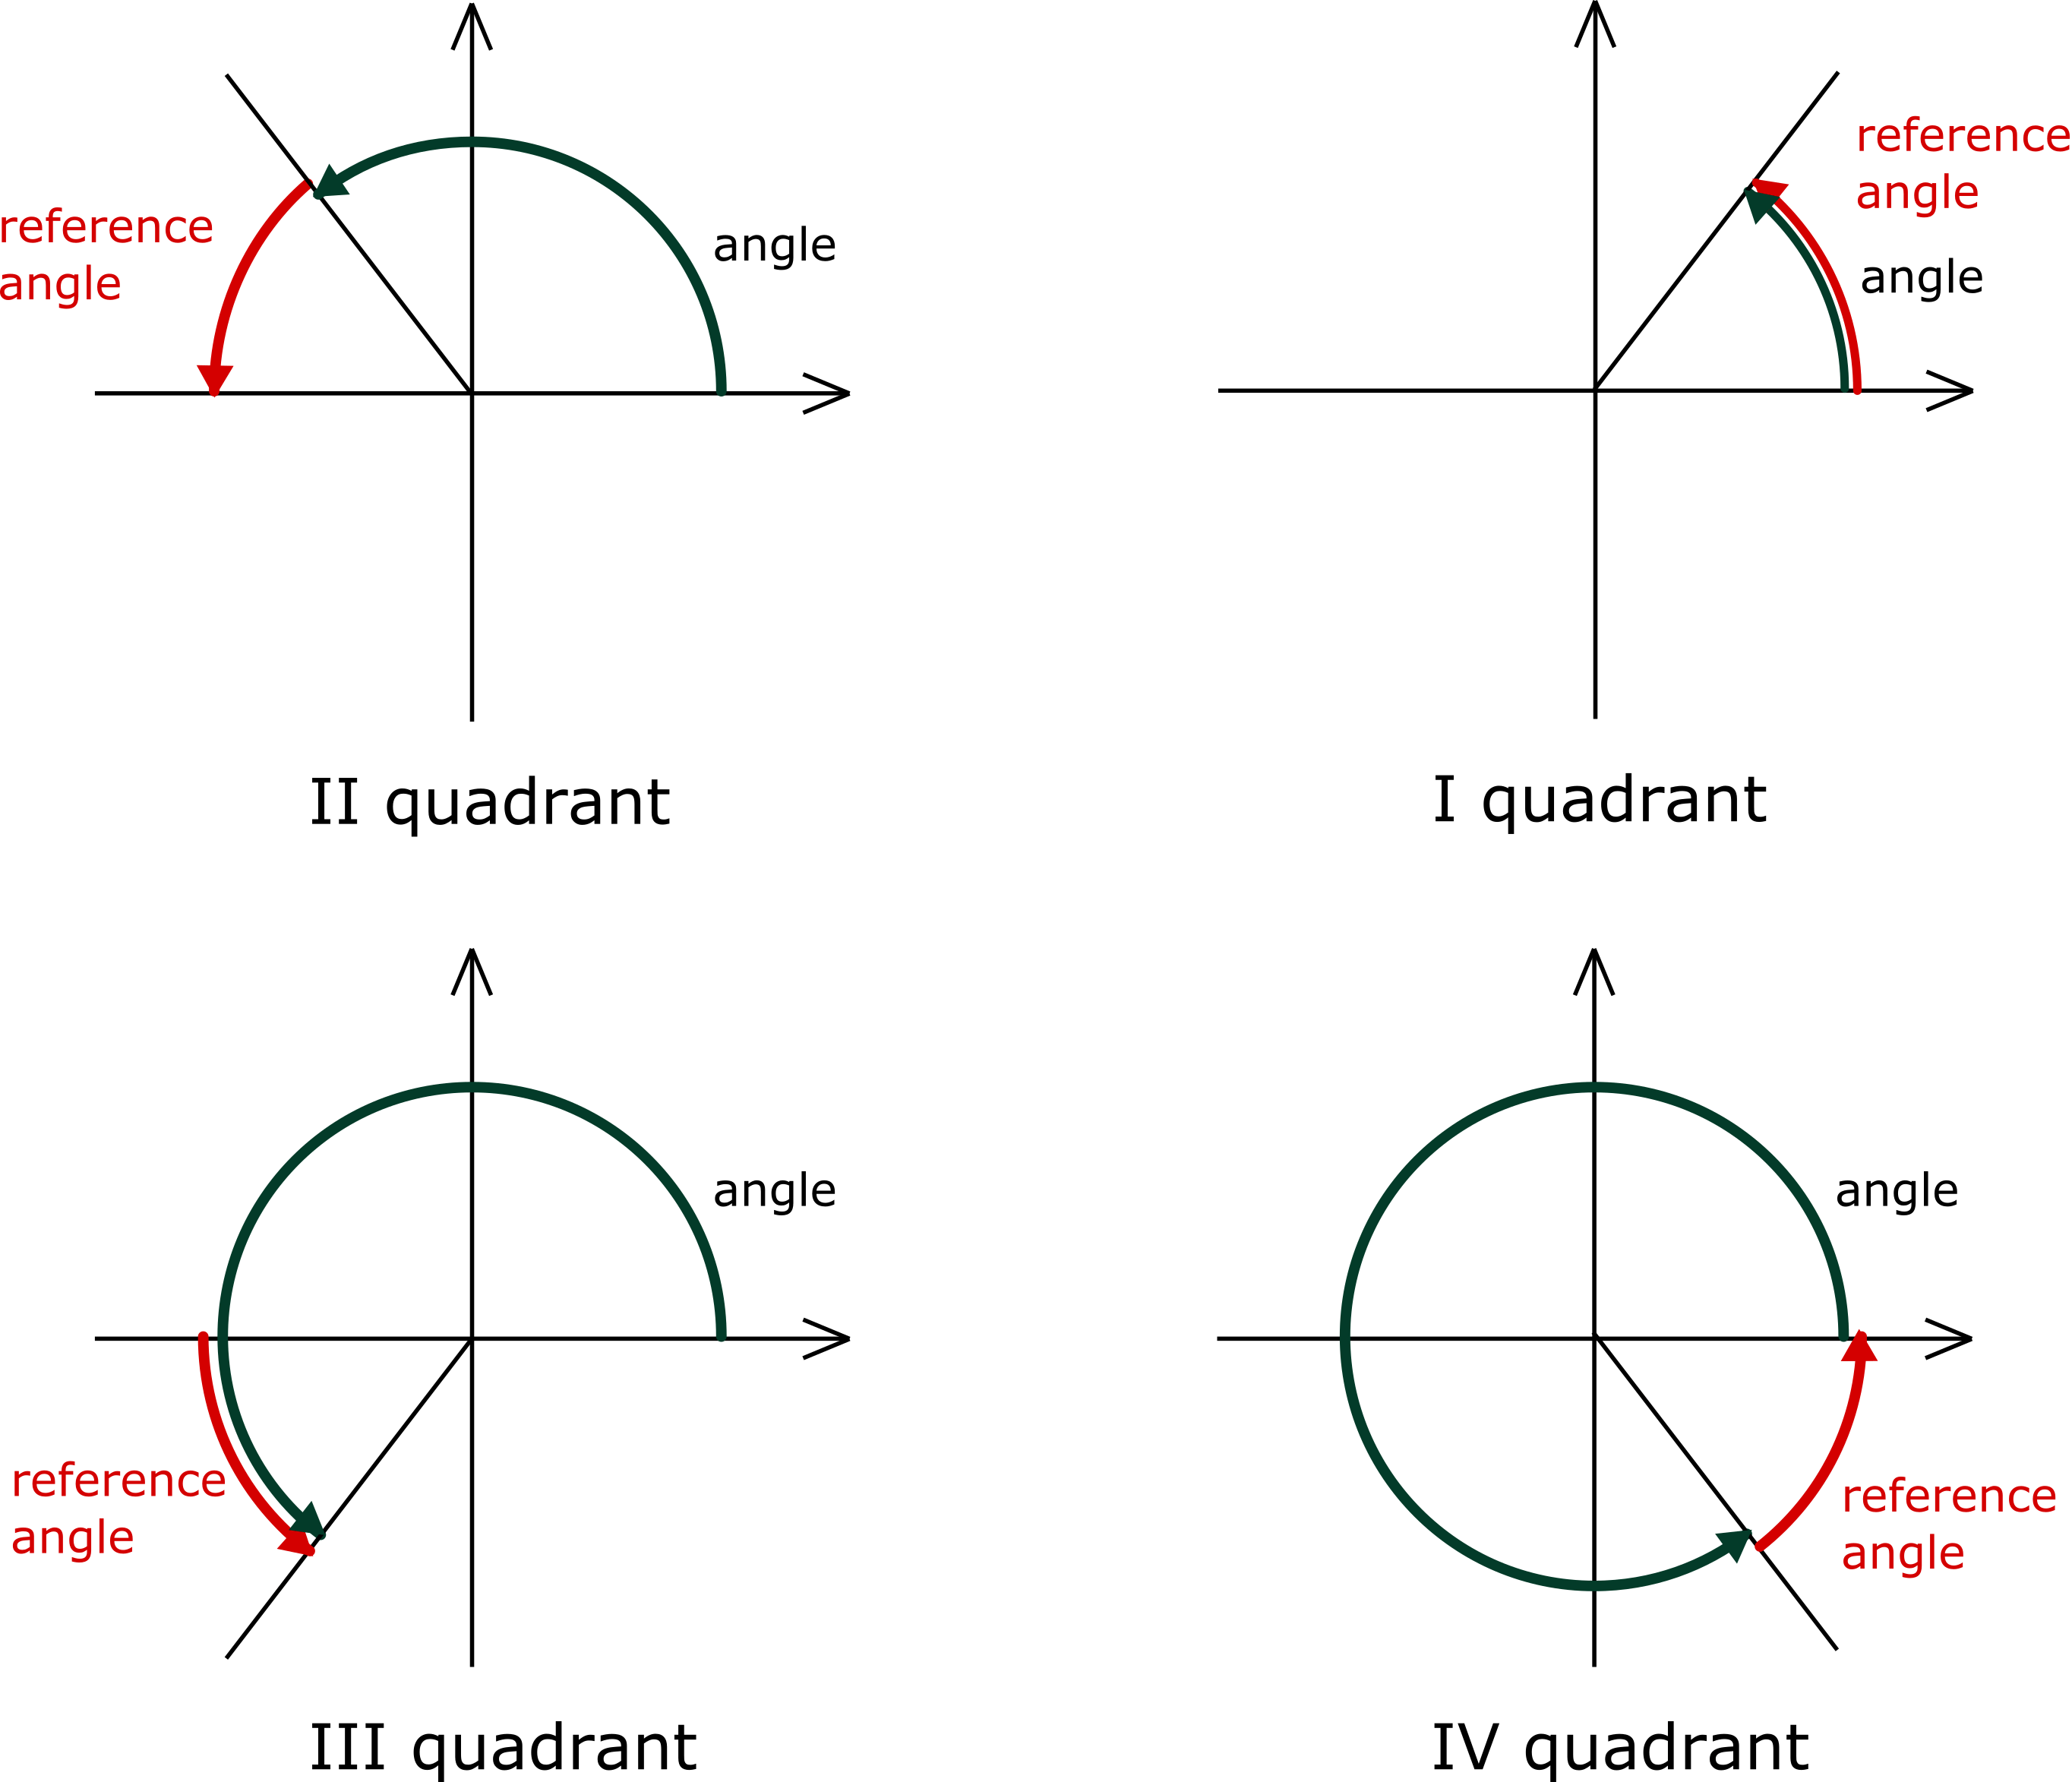
\includegraphics[scale=0.13]{PreCalcPictures/ReferenceAngle.png}}
If we draw a line from the origin to a point $(x,y)$, we can form a triangle and express trig ratios in terms of $x$ and $y$.
$$\sin\theta=\frac{y}{r},\,\cos\theta=\frac{x}{r},\,\tan\theta=\frac{y}{x}$$
Depending which quadrant we are in, these ratios will either be positive or negative.
\begin{align*}
    &\mathrm{QI:}\,\sin\theta>0,\,\cos\theta>0,\,\tan\theta>0\\
    &\mathrm{QII:}\,\sin\theta>0,\,\cos\theta<0,\,\tan\theta<0\\
    &\mathrm{QIII:}\,\sin\theta<0,\,\cos\theta<0,\,\tan\theta>0\\
    &\mathrm{QIV:}\,\sin\theta<0,\,\cos\theta>0,\,\tan\theta<0
\end{align*}

\subsubsection{Primary Trigonometric Functions}
To further simplify, these trig ratios, we can define the unit circle: a circle with radius 1 centered at the origin. This allows us to express any point on the circle in terms of sines and cosines.\\
$(x,y)=(\cos\theta,\sin\theta)$\\
In doing this, we can define $\sin\theta$ to be the height of the circle and $\cos\theta$ as the horizontal component of the circle.\\
\centerline{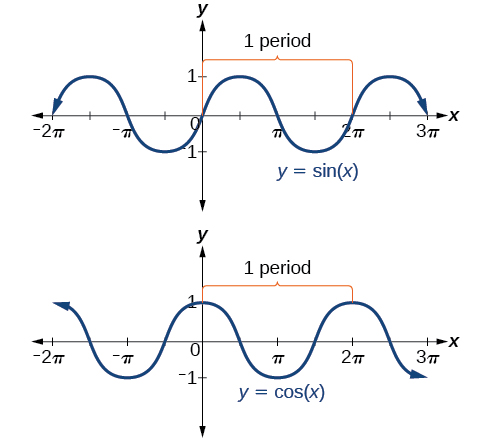
\includegraphics[scale=1.2]{PreCalcPictures/SinxandCosx.jpg}}
Both functions are called sinusoidal curves because they resemble waves. The only difference between the two is that they are shifted over from another by $\frac{\pi}{2}$. They share a common domain and have a range of $y\in[-1,1]$\\
$y=\sin x$ has x-intercepts every $n\pi,\,n\in\mathbb{Z}$\\
$y=\cos x$ has intercepts every $\frac{\pi}{2}+n\pi,\, n\in \mathbb{Z}$\\
The equations in general form are
$$y=a\sin\left(\frac{1}{b}(x-c)\right)+d\text{ and }y=a\cos\left(\frac{1}{b}(x-c)\right)+d$$
Definitions:
\begin{itemize}
    \item Periodic Function: A function that repeats in a regular pattern over a regular interval
    \item Sinusoidal Curve: Curves whose graphs look like waves
    \item Cycle: Portion of a graph to the point it repeats
    \item Period: Length across the x-axis for one cycle
    \item Amplitude: Half the distance between the minimum and maximum values
    \item $d$ is vertical displacement
    \item $c$ is phase shift
    \item $a$ is amplitude
    \item $b$ is change in period
\end{itemize}
Sine and cosine have periods of $2\pi b$.\\ Tangent is defined as $\tan x=\dfrac{\sin x}{\cos x}$ and has a period of $\pi b$\\
\centerline{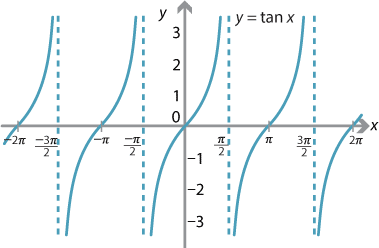
\includegraphics[scale=0.9]{PreCalcPictures/tanx.png}}
$\tan x$ has vertical asymptotes every $x=\frac{\pi}{2}+n\pi,\,n\in\mathbb{Z}$ and x-intercepts every $\pi n,\,n\in\mathbb{Z}$

\subsubsection{Reciprocal Trigonometric Functions}
The reiprocals of trig functions are defined as
$$\csc\theta = \frac{1}{\sin\theta},\,\sec\theta=\frac{1}{\cos\theta},\,\cot\theta=\frac{1}{\tan\theta}=\frac{\cos\theta}{\sin\theta}$$
They will have vertical asymptotes any place where the original function had a zero and they will have x-intercepts any place where the original function had a vertical asymptote.\\
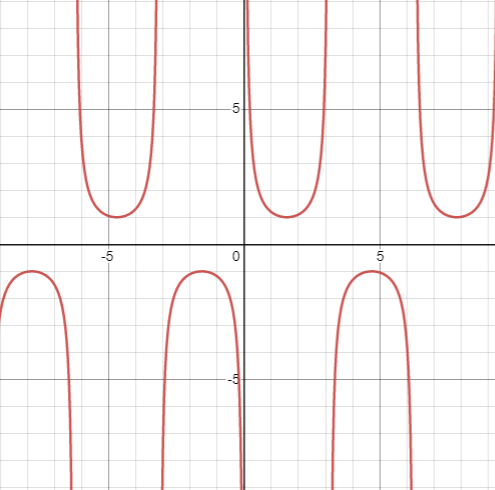
\includegraphics[scale=0.4]{PreCalcPictures/Cscx.png}\
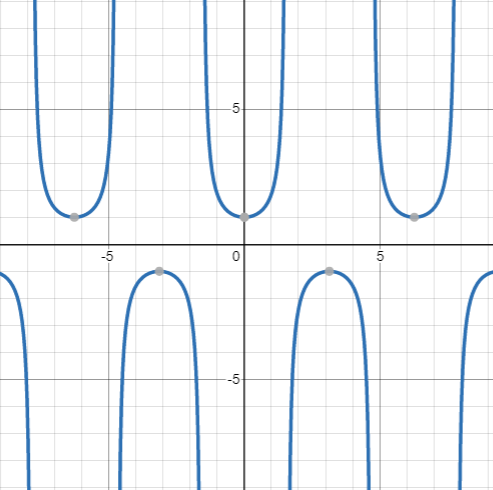
\includegraphics[scale=0.4]{PreCalcPictures/Secx.png}\
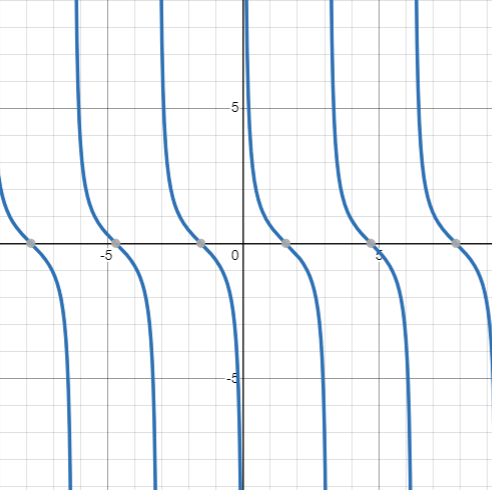
\includegraphics[scale=0.4]{PreCalcPictures/Cotx.png}\\
Shown in order of $\csc x,\,\sec x,\,\cot x$

\subsubsection{Trigonometric Identities}
Pythagorean Identities:\\
These identities can be derived from the unit circle from where $x^2+y^2=1$ and $\cos\theta = x$ and $\sin\theta=y$ so we get
$$\sin^2\theta+\cos^2\theta=1$$
By dividing by $\sin^2\theta$ we get
$$1+\cot^2\theta=\csc^2\theta$$
By dividing by $\cos^2\theta$ we get 
$$\tan^2\theta+1=\sec^2\theta$$
Even-Odd Identities:
\begin{align*}
    \sin(-\theta)&=-\sin\theta\\
    \csc(-\theta)&=-\csc\theta\\
    \tan(-\theta)&=-\tan\theta\\
    \cot(-\theta)&=-\cot\theta\\
    \cos(-\theta)&=\cos\theta\\
    \sec(-\theta)&=\sec\theta
\end{align*}
Co-Function Identities:
\begin{align*}
    \sin\left(\frac{\pi}{2}-\theta\right)&=\cos\theta\\
    \cos\left(\frac{\pi}{2}-\theta\right)&=\sin\theta\\
    \csc\left(\frac{\pi}{2}-\theta\right)&=\sec\theta\\
    \sec\left(\frac{\pi}{2}-\theta\right)&=\csc\theta\\
    \tan\left(\frac{\pi}{2}-\theta\right)&=\cot\theta\\
    \cot\left(\frac{\pi}{2}-\theta\right)&=\tan\theta
\end{align*}
Sum-Difference Identities:
\begin{align*}
    \sin(A\pm B)&=\sin A\cos B\pm \cos A\sin B\\
    \cos(A\pm B)&=\cos A\cos B\mp \sin A\sin B\\
    \tan(A\pm B)&=\frac{\tan A\pm \tan B}{1\mp\tan A\tan B}
\end{align*}
Double Angle Formulas:\\
These are derived from the sum-difference identities.
\begin{align*}
    \sin(2\theta)&=2\sin\theta\cos\theta\\
    \cos(2\theta)&=\cos^2\theta-\sin^2\theta\\
    &=2\cos^2\theta-1\\
    &=1-2\sin^2\theta\\
    \tan(2\theta)&=\frac{2\tan\theta}{1-\tan^2\theta}
\end{align*}
Power Reducing Formulas:
These are derived from the double angle formulas.
\begin{align*}
    \sin^2\theta&=\frac{1-\cos(2\theta)}{2}\\
    \cos^2\theta&=\frac{1+\cos(2\theta)}{2}\\
    \tan^2\theta&=\frac{1-\cos(2\theta)}{1+\cos(2\theta)}
\end{align*}
Sum to Product Formulas:
\begin{align*}
    \sin A+\sin B&=2\sin\left(\frac{A+B}{2}\right)\cos\left(\frac{A-B}{2}\right)\\
    \sin A-\sin B&=2\cos\left(\frac{A+B}{2}\right)\sin\left(\frac{A-B}{2}\right)\\
    \cos A+\cos B&=2\cos\left(\frac{A+B}{2}\right)\cos\left(\frac{A-B}{2}\right)\\
    \cos A-\cos B&=-2\sin\left(\frac{A+B}{2}\right)\sin\left(\frac{A-B}{2}\right)
\end{align*}
Product to Sum Formulas:
\begin{align*}
    \sin A\sin B&=\frac{1}{2}(\cos(A-B)-\cos(A+B))\\
    \sin A\cos B&=\frac{1}{2}(\sin(A+B)+\sin(A-B))\\
    \cos A\cos B&=\frac{1}{2}(\cos(A-B)+\cos(A+B))
\end{align*}
\\
Trig Proofs:\\
Ex: Prove the following:
\begin{align*}
    \tan x\sin x&=\sec x-\cos x\\
    &=\frac{1}{\cos x}-\cos x\left(\frac{\cos x}{\cos x}\right)\\
    &=\frac{1}{\cos x}-\frac{\cos^2x}{\cos x}\\
    &=\frac{1-\cos^2x}{\cos x}\\
    &=\frac{\sin^2x}{\cos x}\\
    &=\tan x\sin x\\
    &\text{Q.E.D.}
\end{align*}
\begin{align*}
    \text{Ex2: }2\cos A\sin B&=\sin(A+B)-\sin(A-B)\\
    &=\sin A\cos B+\sin B\cos A-(\sin A\cos B-\sin B\cos A)\\
    &=\sin B\cos A+\sin B\cos A\\
    &=2\cos A\sin B\\
    &\text{Q.E.D.}
\end{align*}

\subsubsection{Solving Trigonometric Equations}
To solve a trig equation, we want to use trig identities to express the equation as a single term.\\
\begin{align*}
    \text{Ex: }&\cos(2x)-\cos x=0\\
    &2\cos^2x-1-\cos x=0\\
    &(2\cos x+1)(\cos x-1)=0\\
    &\Ra\cos x=\left\{-\frac{1}{2},1\right\}\\
    &x_R=\pi-\frac{\pi}{3}=\frac{2\pi}{3}\\
    &x_R=\pi+\frac{\pi}{3}=\frac{4\pi}{3}\\
    &x_R=0\\
    &\Ra x=\left\{0,\frac{2\pi}{3},\frac{4\pi}{3}\right\}+2\pi n,\,n\in\mathbb{Z}
\end{align*}
\begin{align*}
    \text{Ex2: }&3\sqrt{3}\sin(3x)-3\cos(3x)=3\sqrt{3}\\
    &3\sqrt{3}\sin(3x)=3\sqrt{3}+3\cos(3x)\\
    &27\sin^2(3x)=27+18\sqrt{3}\cos(3x)+9\cos^2(3x)\\
    &3(1-\cos^2(3x))=3+2\sqrt{3}\cos(3x)+\cos^2(3x)\\
    &3-3\cos^2(3x)=3+2\sqrt{3}\cos(3x)+\cos^2(3x)\\
    &4\cos^2(3x)+2\sqrt{3}\cos(3x)=0\\
    &\cos(3x)(4\cos(3x)+2\sqrt{3})=0\\
    &\cos(3x)=0\Ra3x=\left\{\frac{\pi}{2},\frac{3\pi}{2}\right\}+2\pi n,\,n\in\mathbb{Z}\\
    &x=\left\{\frac{\pi}{6},\frac{\pi}{2}\right\}+\frac{2\pi}{3}n,\,n\in\mathbb{Z}\\
    &4\cos(3x)+2\sqrt{3}=0\Ra\cos(3x)=\frac{\sqrt{3}}{2}\Ra3x=\left\{\frac{5\pi}{6},\frac{7\pi}{6}\right\}+2\pi n,\,n\in\mathbb{Z}\\
    &x=\left\{\frac{5\pi}{18},\frac{7\pi}{18}\right\}+\frac{2\pi}{3}n,\,n\in\mathbb{Z}\\
    &\text{Because we squared both sides we may have introduced extraneous roots.}\\
    &\text{To check this, we can plug in the values or solve for the $\sin x$ case}\\
    &\text{and take the $x$ values that satisfy both.}\\
    &3\sqrt{3}\sin(3x)-3\cos(3x)=3\sqrt{3}\\
    &3\sqrt{3}\sin(3x)-3\sqrt{3}=3\cos(3x)\\
    &27\sin^2(3x)-54\sin(3x)+27=9(1-\sin^2(3x))\\
    &3\sin^2(3x)-6\sin(3x)+3=1-\sin^2(3x)\\
    &4\sin^2(3x)-6\sin(3x)+2=0\\
    &\sin(3x)=\frac{1}{2}\Ra3x=\left\{\frac{\pi}{6},\frac{5\pi}{6}\right\}+2\pi n,\,n\in\mathbb{Z}\\
    &\sin(3x)=1\Ra3x=\frac{\pi}{2}+2\pi n,\,n\in\mathbb{Z}\\
    &x=\left\{\frac{\pi}{18},\frac{\pi}{6},\frac{5\pi}{18}\right\}+\frac{2\pi}{3}n,\,n\in\mathbb{Z}\\
    &\therefore\,x=\left\{\frac{\pi}{6},\frac{5\pi}{18}\right\}+\frac{2\pi}{3}n,\,n\in\mathbb{Z}
\end{align*}
\subsubsection{Inverse Trigonometric Functions}
If we take the inverse of a trigonometric function, it would not pass the vertical line test and would not be a function. To get around this, we need to restrict the domain in which we take the inverse.\\
The value from the appropriate range that an inverse function returns is called the principal value of the function.\\
Graphs:\\
\centerline{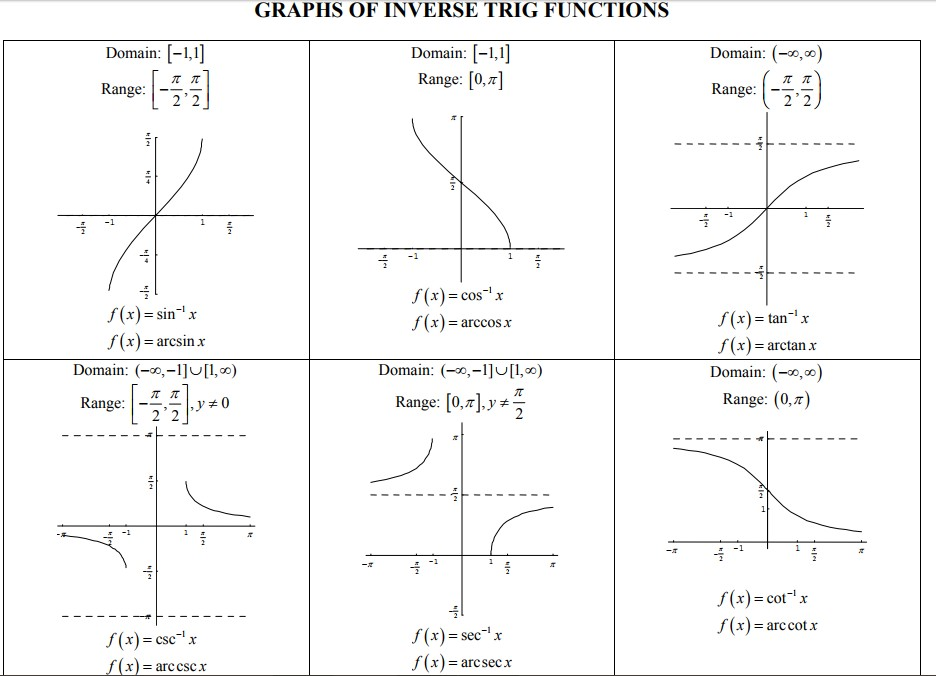
\includegraphics[scale=0.5]{PreCalcPictures/InverseTrigGraphs.png}}

Identities:
\begin{align*}
    &\text{even/odd: }\\
    &\arcsin (-x)=-\arcsin x\\
    &\arccos(-x)=\pi-\arccos x\\
    &\arctan(-x)=-\arctan x\\
    &\arccot(-x)=\pi-\arccot x\\
    &\arccsc(-x)=-\arccsc x\\
    &\arcsec(-x)=\pi-\arcsec x\\
    &\text{Reciprocal:}\\
    &\arcsec x=\arccos\left(\frac{1}{x}\right)\\
    &\arccsc x=\arcsin\left(\frac{1}{x}\right)\\
    &\arccot x=\displaystyle{\left\{\begin{matrix}
    \arctan\left(\frac{1}{x}\right)\text{ if }x\geq 0\\
    \pi+\arctan\left(\frac{1}{x}\right)\text{ if }x<0
    \end{matrix}\right.}\\
    &\arccot x=\frac{\pi}{2}-\arctan x
\end{align*}
Because of the restricted domain, we need to be careful with inverse trig functions.\\
Ex: $\arcsin(\sin(\pi))=\arcsin(0)=0$\\
While $\sin(\arcsin(\pi))$ is undefined.\\
To get around this, we can add or subtract increments of $2\pi$ to get our value within the appropriate range.\\
Ex2: $\arcsin\left(\sin\left(\frac{13\pi}{3}\right)\right)=\arcsin\left(\sin\left(\frac{\pi}{3}\right)\right)=\frac{\pi}{3}$\\
For more complicated examples, we can visualise it with a triangle.\\
Ex3: $\cos(\arcsin x)$\\
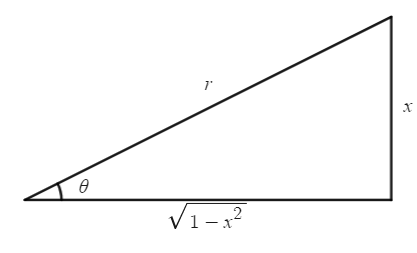
\includegraphics[scale=0.5]{PreCalcPictures/TriangleInvTrig.png}
\begin{align*}
    &\text{let }\theta=\arcsin x\Ra x=\sin\theta\\
    &\Ra\cos\theta=\sqrt{1-x^2}\\
    &\cos(\arcsin x)=\sqrt{1-x^2}
\end{align*}













\subsection{Complex Numbers}
Complex numbers arise from the roots of polynomials.\\
Ex: $x^2+1=0\Ra x^2=-1 \Ra x=\pm\sqrt{-1}$. This polynomial has no real roots, however, we can introduce an imaginary number $i$ such that $i^2=-1$. Then we will have the solution $x=\pm i$\\
We can introduce \textit{complex numbers} which are numbers in the form $z=x+iy$, where $x$ is the real part of $z$, $\Re(z)$, and $y$ is the imaginary part of $z$, $\Im(z)$. 
These numbers can also be expressed in vector notation along the complex plane.\\
Complex Arithmetic:\\
Addition, subtraction, and multiplication works the same, just with the addition of the fact $i^2=-1$. For division, we require what is called the conjugate.\\
The conjugate of a complex number is the same number, just with the sign of the imaginary component flipped.
$$\overline{z}=x-yi$$
where $\overline{z}$ is the conjugate of $z$.\\
Similarly to vectors, we can also define the modulus (length) of a complex number
$$|z|^2=x^2+y^2=z\cdot\overline{z}$$
Using this, we can define division of a complex number and also define the real and imaginary components of a complex number.
\begin{align*}
    &\frac{u}{z}=\frac{s+it}{x+iy}=\frac{(s+it)(x-iy)}{(x+iy)(x-iy)}=\frac{u\overline{z}}{x^2+y^2}=\frac{u\overline{z}}{|z|^2}
\end{align*}
Another way to represent complex numbers is through polar form. To use this we must first introduce Euler's identity:
$$e^{i\theta}=\cos\theta+i\sin\theta$$
This then helps us with the equation for polar form
$$z=a+ib=|z|(\cos\theta+i\sin\theta)=|z|e^{i\theta}$$
Ex: Represent $1+i$ in polar coordinates
\begin{align*}
    &|z|=\sqrt{2}\\
    &\theta=\arctan{\frac{b}{a}}=\arctan{1}=\frac{\pi}{4}\\
    &z=\sqrt{2}e^{\frac{\pi i}{4}+2n},\,n\in\R
\end{align*}
Ex2: Find the roots of $x^3=2$
\begin{align*}
    &x=|x|e^{i\theta}\\
    &|x|=\sqrt[3]{2}\\
    &x^3=2=2e^{3i\theta}\Ra 1=e^{3i\theta}=\cos(3\theta)+i\sin(3\theta)\\
    &\Ra \cos(3\theta)=1\\
    &3\theta=2\pi n,\,n\in\R\\
    &\theta=\frac{3\pi}{2}n,\,n\in\R\\
    &x=\eqnsystem{\sqrt[3]{2}\\\sqrt[3]{2}e^{i\frac{2\pi}{3}}\\\sqrt[3]{2}e^{i\frac{4\pi}{3}}}
\end{align*}















































% Differential calculus





\section{Differential Calculus}

\subsection{Limits and Continuity}

\subsubsection{Limit Definition}
The limit of a function at a point is the value that function approaches, regardless of whether it actually achieves that value. This makes limits particularly useful for determining what a function does at places it is not defined.\\
For example, the function $\frac{x^2+4x+3}{x+1}$ is undefined at $x=-1$, however, we can take the limit as $x$ approaches $-1$ to see what value the function approaches:
\begin{align*}
    \lim \limits_{x\to -1}\frac{x^2+4x+3}{x+1}\\
    f(-1.1)= 1.9\\
    f(-0.9)= 2.1\\
    f(-1.01)= 1.99\\
    f(-0.99)= 2.01
\end{align*}
As we can see, as we get closer and closer to $x=-1$ the value of $f(x)$ approaches $2$ so we can say that $\lim \limits_{x\to -1}\frac{x^2+4x+3}{x+1}=2$\\
\\
The limit of a function exists such that if $\lim\limits_{x\to a}f(x)=L$ there exists a positive number $\delta$ such that $|f(x)-L|<\varepsilon$ is true for $|x-a|<\delta$\\
Ex: Determine if $\lim\limits_{5x-3}=2$
\begin{align*}
    &f(x)=5x-3,\,a=1,\,L=2\\
    &|x-1|<\delta\\
    &|5x-3-3|<\varepsilon\\
    &|5x-5|<\varepsilon\\
    &5|x-1|<\varepsilon\\
    &|x-1|<\frac{\varepsilon}{5}\\
    &\Ra\delta=\frac{\varepsilon}{5}
\end{align*}
More conceptually, we can say that a limit exists if the right hand and left hand limits approach the same value.\\
i.e. $\lim\limits_{x\to a^+}f(x)=\lim\limits_{x\to a^-}f(x)$\\
Ex: $\lim\limits_{x\to 0^+}\frac{1}{x}=\infty$\\
but $\lim\limits_{x\to 0^-}\frac{1}{x}=-\infty$\\
$\therefore\,\lim\limits_{x\to 0}\frac{1}{x}$ does not exist\\
Ex2: $\lim\limits_{x\to 0^+}\frac{1}{x^2}=\infty$\\
and $\lim\limits_{x\to 0^-}\frac{1}{x^2}=\infty$\\
$\therefore\,\lim\limits_{x\to 0}=\infty$

\subsubsection{Limit Arithmetic}
With limits, we have the following properties:\\
For $\lim\limits_{x\to a}f(x)=l$ and $\lim\limits_{x\to a}g(x)=M$
$$\lim_{x\to a}(f(x)\pm g(x))=\lim_{x\to a}f(x)\pm\lim_{x\to a}g(x)=L\pm M$$
$$\lim_{x\to a}(cf(x))=c\lim_{x\to a}f(x)=cL$$
$$\lim_{x\to a}(f(x)g(x))=\lim_{x\to a}f(x)\lim_{x\to a}g(x)=LM$$
$$\lim_{x\to a}\left(\frac{f(x)}{g(x)}\right)=\frac{\lim\limits_{x\to a}f(x)}{\lim\limits_{x\to a}g(x)}=\frac{L}{M}$$
$$\lim_{x\to a}(f(x))^n=(\lim_{x\to a}f(x))^n=L^n$$
$$\lim_{x\to a}\sqrt[n]{f(x)}=\sqrt[n]{\lim_{x\to a}f(x)}=\sqrt[n]{L}$$
$$\lim_{x\to a}e^{f(x)}=e^{\lim\limits_{x\to a}f(x)}=e^L$$
\\
Limits at Infinity:\\
Ex: $\lim\limits_{x\to\infty}\frac{1}{x}=0$\\
Ex2: $\lim\limits_{x\to\infty}\frac{2x^2}{5x^2-3}$
\begin{align*}
    &=\lim\limits_{x\to\infty}\frac{2x^2}{5x^2-3}\left(\frac{1/x^2}{1/x^2}\right)\\
    &=\lim\limits_{x\to\infty}\frac{2}{5-\frac{3}{x^2}}\\
    &=\frac{2}{5}
\end{align*}
Ex3: $\lim\limits_{x\to-\infty}\frac{x+6}{\sqrt{16x^2-7}}$
\begin{align*}
    &=\lim\limits_{x\to-\infty}\frac{x+6}{\sqrt{16x^2-7}}\left(\frac{1/|x|}{1/|x|}\right)\\
    &=\lim\limits_{x\to-\infty}\frac{(x+6)\frac{1}{-x}}{\sqrt{16x^2-7}\frac{1}{\sqrt{x^2}}}\\
    &=\lim\limits_{x\to-\infty}\frac{-1-\frac{6}{x}}{\sqrt{16-\frac{7}{x^2}}}\\
    &=-\frac{1}{4}
\end{align*}\\
Squeeze Theorem:\\
If $g(x)\leq f(x)\leq h(x)$ and $\lim\limits_{x\to a}g(x)=\lim\limits_{x\to a}=L$ then $\lim\limits_{x\to a} f(x)=L$\\
Ex: $\lim\limits_{x\to 0}\dfrac{\sin x}{x}$\\
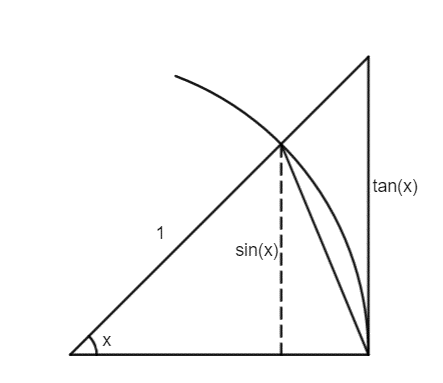
\includegraphics[scale =0.6]{DifferentialCalculusPictures/limitTriangle.png}
\begin{align*}
    &\text{Area of segment: }\frac{x}{2}\\
    &\text{Area of big triangle: }\frac{\tan x}{2}\\
    &\text{Area of small triangle: } \frac{\sin x}{2}\\
    &\frac{\sin x}{2}\leq\frac{x}{2}\leq\frac{\tan x}{2}\\
    &\frac{1}{\sin x}\leq\frac{1}{x}\leq\frac{1}{\tan x}\\
    &=\frac{\sin x}{\sin x}\leq\frac{\sin x}{x}\leq \frac{\sin x}{\tan x}\\
    &=1\leq\lim_{x\to 0}\frac{\sin x}{x}\leq\lim_{x\to 0}\cos x\\
    &\therefore\,\lim_{x\to 0}\frac{\sin x}{x}=1
\end{align*}
Ex2: $\lim\limits_{x\to 0}\frac{\cos x-1}{x}$
\begin{align*}
    \lim\limits_{x\to 0}\frac{\cos x-1}{x}&=\lim_{x\to 0}\frac{-2\sin^2\left(\frac{x}{2}\right)}{x}\\
    &=\lim_{\frac{x}{2}\to 0}\frac{-\sin^2\left(\frac{x}{2}\right)}{\frac{x}{2}}\\
    &=\lim_{\frac{x}{2}\to 0}-\sin\left(\frac{x}{2}\right)\frac{\sin\left(\frac{x}{2}\right)}{\frac{x}{2}}\\
    &=0
\end{align*}
Now, a more general case:
\begin{align*}
    \text{Ex3: }&\lim_{x\to 0}\frac{\sin(ax)}{x}\\
    &\text{We know }\lim_{x\to 0}\frac{\sin x}{x}=1\\
    &\text{and }ax\to 0\Longleftrightarrow x\to 0\\
    &\text{so }\lim_{x\to 0}\frac{\sin(ax)}{ax}=1\\
    &\Ra\lim_{x\to 0}\frac{\sin(ax)}{x}=a
\end{align*}

\subsubsection{Continuity}
A function is said to be continuous at a point $c$ if the following three conditions are satisfied:
\begin{enumerate}
    \item $f(c)$ exists
    \item $\lim\limits_{x\to c}f(x)$ exists
    \item $\lim\limits_{x\to c}f(x)=f(c)$
\end{enumerate}
If $f(x)$ and $g(x)$ are continuous then the composition of $f$ and $g$ is also continuous.\\
The conditions of the derivative state that the function must be continuous. So if the derivative of a function is continuous, the original function must also be continuous.\\
Note that a continuous function does not always give a continuous derivative.\\
Ex: Find a real number $a$ such that $f(x)$ is continuous 
\begin{align*}
    &f(x)=\left\{\begin{matrix}
    \frac{x^2-9}{x+a},\, x<-a\\
    x+3,\,x\geq-a
    \end{matrix}\right.\\
    &\text{We need }\lim_{x\to-a^-}\frac{x^2-9}{x+a}=\lim_{x\to-a^+}(x+3)=-a+3\\
    &\lim_{x\to -a^-}\frac{(x+3)(x-3)}{x+a}=-a+3\\
    &\frac{(-a+3)(-a-3)}{\lim\limits_{x\to-a^-}(x+a)}=a+3\\
    &\Ra-a-3=\lim_{x\to-a^-}(x+a)=0\\
    &\Ra a=-3
\end{align*}












\subsection{Differentiation}

\subsubsection{Tangent Lines}
We are often interested in rates of change. We know the rate of change of a linear function to be its slope which is a constant. However, for nonlinear functions, the rate of change is not constant. We can determine the instantaneous rate of change of a function at a point $P$ by drawing a line tangent to the curve at that point. This line is not always easy to find so we start by drawing a secant line that intersects the curve at two points, $P$ and $Q$.\\
\centerline{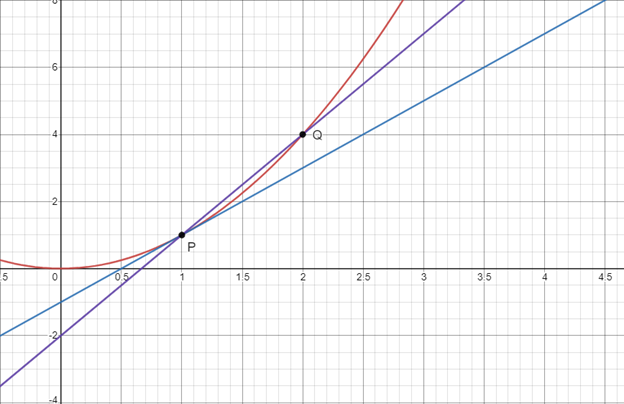
\includegraphics[scale =0.7]{DifferentialCalculusPictures/Tangent.png}}
To find the tangent line, we can take the limit as the point $Q$ on the secant line approaches the point $P$.\\
The slope of the secant line is $m_{sec}=\dfrac{f(x_Q)-f(x_P)}{x_Q-x_P}$\\
We can define $x_Q=x_P+h$ where $h$ is the distance between the points so,\\ ${m_{sec}=\dfrac{f(x_P+h)-f(x_P)}{x_P+h-x_P}=\dfrac{f(x_P+h)-f(x_P)}{h}}$\\
Because we are interested in the case where $x_P=x_Q$, we take the limit as $h\to 0$:\\
$m_{tan}=\displaystyle{\lim \limits_{h\to 0}\dfrac{f(x_P+h)-f(x_P)}{h}}$\\
This is in fact the definition of the derivative. Put simply, the derivative measures rates of change between two variables. It is denoted by $f'(x)$ or $\frac{dy}{dx}$.\\
$$f'(x)=\lim\limits_{h\to 0}\frac{f(x+h)-f(x)}{h}=\lim_{x\to a}\frac{f(x)-f(a)}{x-a}$$
So, the tangent line at a point $a$ can be defined as $$y=f'(a)x+f(a)$$
Ex: Find the line tangent to $x^3$ at $(2,8)$
\begin{align*}
    &f'(2)=\lim\limits_{h\to 0}\frac{(2+h)^3-2^3}{h}=\lim\limits_{h\to 0}\frac{8+12h+6h^2+h^3-8}{h}=\lim\limits_{h\to 0}(12+6h+h^2)=12\\
    &y=f'(2)x+f(2)=12x+8
\end{align*}
It is important to note that a function must be continuous in order for it to be differentiable.

\subsubsection{Derivative Laws}
We can derive various derivative laws that will make calculating derivatives far easier. They stem from these derivations:\\
Derivative of a Constant:
\begin{align*}
    \frac{d}{dx}c&=\lim_{h\to 0}\frac{c-c}{h}\\
    \frac{d}{dx}c&=0
\end{align*}
Derivative of a Polynomial:
\begin{align*}
    \frac{d}{dx}x^n&=\lim\limits_{h\to 0}\frac{(x+h)^n-x^n}{h}\text{ for $n$ is a constant}\\
    \text{Binomial theorem: }& (a+b)^n=\prescript{}{n}{C}_0a^n+\prescript{}{n}{C}_1a^{n-1}b+\prescript{}{n}{C}_2a^{n-2}b^2+\cdots+\prescript{}{n}{C}_{n-1}ab^{n-1}+\prescript{}{n}{C}_nb^n\\
    \frac{d}{dx}x^n&=\lim\limits_{h\to 0}\frac{x^n+nx^{n-1}h+\cdots+nh^{n-1}+h^n-x^n}{h}\\
    \frac{d}{dx}x^n&=\lim\limits_{h\to 0}(nx^{n-1}+n(n-1)x^{x-2}h+\cdots+h^{n-1})\\
    \frac{d}{dx}x^n&=nx^{n-1}
\end{align*}
Ex: $\frac{d}{dx}(6x^5)=30x^4$\\
Note that coefficients do not change the value of the derivative. I did not prove this but it's easy to see.\\
Ex2: $\frac{d}{dx}\sqrt{x}=\frac{1}{2}x^{-\frac{1}{2}}=\frac{1}{2\sqrt{x}}$\\
We can define the multiplication of two functions with the product rule:
\begin{align*}
    \frac{d}{dx}(f(x)g(x))&=\lim_{h\to 0}\frac{f(x+h)g(x+h)-f(x)g(x)}{h}\\
    &=\lim_{h\to 0}\frac{f(x+h)g(x+h)-f(x)g(x)-f(x)g(x+h)+f(x)g(x+h)}{h}\\
    &=\lim_{h\to 0}\left(f(x)\frac{g(x+h)-g(x)}{h}+g(x+h)\frac{f(x+h)-f(x)}{h}\right)\\
    &=f(x)g'(x)+g(x)f'(x)
\end{align*}
Product Rule with 3 Functions:
\begin{align*}
    (uvw)'=u'vw+v'uw+w'uv
\end{align*}
Quotient Rule:
\begin{align*}
    \frac{d}{dx}\left(\frac{f(x)}{g(x)}\right)&=\lim_{h\to 0}\frac{\frac{f(x+h)}{g(x+h)}-\frac{f(x)}{g(x)}}{h}\\
    &=\lim_{h\to 0}\frac{g(x)f(x+h)-f(x)g(x+h)}{hg(x)g(x+h)}\\
    &=\lim_{h\to 0}\frac{g(x)f(x+h)-f(x)g(x+h)+g(x+h)f(x+h)-g(x+h)f(x+h)}{hg(x)g(x+h)}\\
    &=\lim_{h\to 0}\frac{g(x+h)\frac{f(x+h)-f(x)}{h}-f(x+h)\frac{g(x+h)-g(x)}{h}}{g(x)g(x+h)}\\
    &=\frac{g(x)f'(x)-f(x)g'(x)}{(g(x))^2}
\end{align*}
Reciprocal Rule:
\begin{align*}
    \frac{d}{dx}\brround{\frac{1}{v}}=-\frac{v'}{v^2}
\end{align*}
Ex: $\dfrac{d}{dx}x^2\cos x=2x\cos x-x^2\sin x$\\
By extension of the quotient rule, we can also define the derivative of a reciprocal to be
$$\frac{d}{dx}\frac{1}{x}=\frac{-1}{x^2}$$
Higher Order Derivatives:\\
This is taking the derivative of a derivative, generally expressed as $$\frac{d}{dx}\brround{\frac{dy}{dx}}=\frac{d^2y}{dx^2}=f''(x)$$
Ex: find $f''(x)$ for $f(x)=x^3-x$
\begin{align*}
    &f'(x)=3x^2-1\\
    &f''(x)=6x
\end{align*}
\begin{align*}
    \text{Ex2: }&\frac{d^n}{dx^n}x^n\\
    &\frac{d}{dx}x^n=nx^{n-1}\\
    &\frac{d^2}{dx^2}x^n=n(n-1)x^{n-2}\\
    &\frac{d^3}{dx^3}x^n=n(n-1)(n-2)x^{n-3}\\
    &\frac{d^{n-1}}{dx^{n-1}}x^n=n(n-1)(n-2)\cdots(3)(2)x^1\\
    &\therefore\frac{d^n}{dx^n}x^n=n!
\end{align*}

\subsubsection{Derivatives of Trigonometric Functions}
Derivative of $\sin x$:
\begin{align*}
    \frac{d}{dx}\sin (x)&=\lim_{h\to 0}\frac{\sin(x+h)-\sin (x)}{h}\\
    &=\lim_{h\to 0}\frac{\sin(x)\cos(h)+\sin(h)\cos(x)-\sin(x)}{h}\\
    &=\sin(x)\lim_{h\to 0}\left(\frac{\cos(h)-1}{h}\right)+\cos(x)\lim_{h\to 0}\left(\frac{sin(h)}{h}\right)\\
    &=\cos(x)
\end{align*}
Derivative of $\cos x$:
\begin{align*}
    \frac{d}{dx}\cos(x)&=\lim_{h\to 0}\frac{\cos(x+h)-\cos(x)}{h}\\
    &=\lim_{h\to 0}\frac{\cos(x)\cos(h)-\sin(x)\sin(h)-\cos(x)}{h}\\
    &=\cos(x)\lim_{h\to 0}\left(\frac{\cos(h)-1}{h}\right)-\sin(x)\lim_{h\to 0}\left(\frac{sin(h)}{h}\right)\\
    &=-\sin(x)
\end{align*}
Derivative of $\tan x$:\\
$\dfrac{d}{dx}\tan x=\dfrac{d}{dx}\dfrac{\sin x}{\cos x}=\dfrac{\cos x\cos x+\sin x\sin x}{\cos^2x}=\dfrac{1}{\cos^2x}=\sec^2x$\\
\\
Derivative of $\csc x$:\\
$\dfrac{d}{dx}\dfrac{1}{\sin x}=-\dfrac{\cos x}{\sin^2 x}=-\csc x\cot x$\\
\\
List of Trig Derivatives:\\
\begin{align*}
    &\frac{d}{dx}\sin x=\cos x &\frac{d}{dx}\csc x = -\csc x\cot x\\
    &\frac{d}{dx}\cos x=-\sin x &\frac{d}{dx}\sec x=\sec x\tan x\\
    &\frac{d}{dx}\tan x =\sec^2 x &\frac{d}{dx}\cot x=-\csc^2 x
\end{align*}

\subsubsection{The Chain Rule}
$$\frac{dy}{dx}=\frac{dy}{du}\frac{du}{dx}$$ or also $$\frac{d}{dx}f(g(x))=f'(g(x))g'(x)$$
This gives us the tools we need to differentiate more complicated functions.
Ex: $\frac{d}{dx}(x^2+5x)^3=(x^2+5x)^3(2x+5)$\\
Ex2: $\frac{d}{dx}\cos(x^2)=-2x\sin(x^2)$\\
Ex3: Find values for $a$ and $b$ such that $f(x)$ is differentiable everywhere:
\begin{align*}
    &f(x)=\left\{\begin{matrix}
    x^3+ax+b,\,x\leq 0\\
    x+x^3\sin\brround{\frac{1}{x}}
    ,\,x>0\end{matrix}\right.\\
    &\text{check that $f(x)$ is continuous at $x=0$}\\
    &\lim_{x\to0^-}f(x)=\lim_{x\to0^+}=f(0)\Ra\lim_{x\to 0^+}\brround{x+x^3\sin\brround{\frac{1}{x}}}=b=0\\
    &\text{chech that $f'(x)$ is continuous at $x=0$}\\
    &\lim_{h\to 0}\frac{f(0+h)-f(0)}{h}\text{ must exist}\\
    &\text{recall }\lim_{x\to 0^-}f(x)=\lim_{x\to0^+}f(x)=f(0)=0\\
    &\therefore \lim_{h\to 0}\frac{f(0+h)-f(0)}{h}=\lim_{h\to0}\frac{f(h)}{h}\\
    &\lim_{h\to 0^-}\frac{h^3+ah}{h}=\lim_{h\to 0^+}\frac{h+h^3\sin\brround{\frac{1}{h}}}{h}\\
    &\lim_{h\to0^-}(h^2+a)=\lim_{h\to0^+}\brround{1+h^2\sin\brround{\frac{1}{h}}}\\
    &a=1\\
    &\to a=1,\,b=0
\end{align*}










\subsection{Differentiation Techniques}

\subsubsection{Implicit Differentiation}
Implicit differentiation allows us to calculate the derivative of an implicitly given function without solving for $y$ explicitly.
\begin{align*}
    \text{Ex: }&4xy^2+3x^2y=2\\
    &\frac{d}{dx}(4xy^2)+\frac{d}{dx}(3x^2y)=\frac{d}{dx}2\\
    &4x(2yy')+4y^2+4x^2y'+3y(2x)=0\\
    &8xyy'+6x^2y'=-4y^2-6xy\\
    &y'(8xy+6x^2)=-4y^2-6xy\\
    &y'=\frac{-4y^2-6xy}{8xy+6x^2}
\end{align*}
\begin{align*}
    \text{Ex2: }&x^2+y^2=1\\
    &2x+2yy'=0\\
    &2yy'=-2x\\
    &y'=-\frac{x}{y}
\end{align*}

\subsubsection{Inverse Functions}
Recall that the inverse of a function is a reflection across the line $y=x$\\
For where $g(x)=f^{-1}(x)$,
$$g'(f(a))=\frac{1}{f'(a)}$$
Ex: Find the derivative of the inverse of $y=x^4$ at $x=2$
\begin{align*}
    &f'(x)=4x^3\\
    &f'(2)=32\\
    &\therefore\,g'(f(2))=\frac{1}{32}\\
    &\text{Proof:}\\
    &g(x)=f^{-1}(x)=x^{\frac{1}{4}}\\
    &g'(x)=\frac{1}{4}x^{-\frac{3}{4}}\\
    &f(2)=16\\
    &g'(16)=\frac{1}{32}
\end{align*}
Ex2: For $g(x)=x+e^{(x+1)^3}$, evaluate $(g^{-1})'(c)$ for where $g^{-1}(c)=-1$
\begin{align*}
    &g(x)=x+e^{(x+1)^3}\\
    &x=g^{-1}(g(x))\\
    &1=(g^{-1})'(g(x))g'(x)\\
    &(g^{-1})'(g(x))=\frac{1}{g'(x)}\\
    &g^{-1}(c)=-1\Ra c=g(-1)\\
    &(g^{-1})'(c)=(g^{-1})'(g(-1))=\frac{1}{g'(-1)}\\
    &g'(x)=1+3(x+1)^2e^{(x+1)^3}\\
    &g'(-1)=1\\
    &(g^{-1})'(c)=\frac{1}{1}=1
\end{align*}
\subsubsection{The Exponential Function}
Derivative of the exponential function $y=a^x$:
\begin{align*}
    &\frac{d}{dx}a^x=\lim_{h\to 0}\frac{a^{x+h}-a^x}{h}\\
    &f'(x)=a^x\lim_{h\to 0}\frac{a^h-1}{h}\\
    &\text{where }\lim_{h\to 0}\frac{a^h-1}{h}=f'(0)\\
    &\text{so }f'(x)=f'(0)f(x)
\end{align*}
By observation, we know by the graph of the function that the derivative $f'(0)$ exists so the derivative of the exponential is itself times some constant.\\
If we want to define a function such that $f'(x)=f(x)$ we need to find the $a$ value that corresponds with a constant of 1.
\begin{align*}
    &f'(0)=\lim_{h\to 0}\frac{a^h-1}{h}\\
    &\text{let }k=a^h-1\\
    &\lim_{h\to 0}=\lim_{k\to 0}\\
    &a^h=k+1\Ra h=\log_a(k+1)\\
    &f'(0)=\lim_{k\to 0}\frac{k}{\log_a(k+1)}=\lim_{k\to 0}\frac{1}{\log_a(k+1)^{1/k}}=1\\
    &\Ra\lim_{k\to 0}\log_a(k+1)^{1/k}=1\\
    &a=\lim_{k\to 0}(k+1)^{1/k}
\end{align*}
Solving this limit is a somewhat circular argument as we need to know what $a$ is to compute it algebraically. Fortunately, we can take small values of $k$ and estimate the limit to be $2.71828\ldots$\\
We will call this value Euler's constant, $e$.\\
So, $\dfrac{d}{dx}e^x=e^x$\\
Euler's constant shows up in a few interesting cases. One common case is in compounding interest:
$$e=\lim_{n\to \infty}\brround{1+\frac{1}{n}}^n$$
\textbf{Applications}\\
Ex: Carbon Dating\\
There is a constant amount of Carbon-14 present in organic matter. Once an organism dies, it stops acquiring Carbon-14. If a plant dies at time $t=0$, the number of micrograms of Carbon-14 is $f(t)=10e^{-kt}$ with the half-life of Carbon-14 being 5730 years. If $1\mu g$ of Carbon-14 remains, when did it die?
\begin{align*}
    &f(5730)=10e^{-5730k}=5\\
    &\frac{1}{2}=e^{-5730k}\\
    &5730k=\ln 2\\
    &k=\frac{\ln 2}{5730}\\
    &10e^{-\frac{\ln 2}{5730}t}=1\\
    &e^{-\frac{\ln 2}{5730}t}=\frac{1}{10}\\
    &\frac{\ln 2}{5730}t=\ln10\\
    &t=5730\frac{\ln10}{\ln2}\approx19030\text{ years}
\end{align*}
Ex2: Newton's Law of Cooling
$$T(t)=(T(0)-A)e^{kt}+A$$
where $A$ is the temperature of the surroundings.\\
A body is discovered at 3:45pm in a locked room held at $20^\circ$. The body's temperature is $27^\circ$. By 5:45pm its temperature has dropped to $25.3^\circ$. When did the person die?
\begin{align*}
    &T(t)=(27-20)e^{kt}+20=7e^{kt}+20\\
    &7e^{2k}+20=25.3\\
    &e^{2k}=\frac{5.3}{7}\\
    &e^k=\sqrt{\frac{5.3}{7}}\\
    &T(t)=7\brround{\frac{5.3}{7}}^{t/2}+20=37\\
    &\brround{\frac{5.3}{7}}^{t/2}=\frac{17}{7}\\
    &t=\frac{2\ln\brround{\frac{17}{7}}}{\ln\brround{\frac{5.3}{7}}}\approx-6.4
\end{align*}
So the person died 6 hours and 24 minutes before 3:45pm.
\subsubsection{Logarithmic Differentiation}
We found that the derivative of $e^x$ is $e^x$. We can use this to determine the derivative of $\ln x$:
\begin{align*}
    &y=\ln x\\
    &x=e^y\\
    &1=e^yy'\\
    &y'=\frac{1}{e^y}\\
    &y'=\frac{1}{x}\\
    &\Ra\frac{d}{dx}\ln x=\frac{1}{x}
\end{align*}
The properties of natural logarithms can be useful to find derivatives of difficult functions.\\
We can introduce a method called logarthmic differentiation:
\begin{enumerate}
    \item Write the equation in the form $y=f(x)$
    \item Take the natural log of both sides
    \item Use properties of logs to simplify the expression
    \item Differentiate the equation implicitly with respect to x
    \item Solve for $y'$
\end{enumerate}
\begin{align*}
    \text{Ex: }y&=\frac{x^2\sqrt{x^2+7}}{\sqrt[3]{x+5}}\\
    \ln y&=\ln\left(\frac{x^2\sqrt{x^2+7}}{\sqrt[3]{x+5}}\right)=\ln x^2+\ln(x^2+7)^\frac{1}{2}-\ln(x+5)^\frac{1}{3}=2\ln x+\frac{1}{2}\ln(x^2+7)-\frac{1}{3}\ln(x+5)\\
    \frac{y'}{y}&=\frac{2}{x}+\frac{1}{2}\frac{2x}{x^2+7}-\frac{1}{3}\frac{1}{x+5}\\
    y'&=y\left(\frac{2}{x}+\frac{x}{x^2+7}-\frac{1}{3(x+5)}\right)=\frac{x^2\sqrt{x^2+7}}{\sqrt[3]{x+5}}\left(\frac{2}{x}+\frac{x}{x^2+7}-\frac{1}{3(x+5)}\right)
\end{align*}
\begin{align*}
    \text{Ex2: }&y=x^x\\
    &\ln y=x\ln x\\
    &\frac{y'}{y}=x\frac{1}{x}+\ln x=1+\ln x\\
    &y'=y(1+\ln x)\\
    &y'=x^x(1+\ln x)
\end{align*}
So far, we have just dealt with logs and exponentials with base $e$. Using logarithmic differentiation, we can define the derivatives for more general cases:
\begin{align*}
    \text{Ex: }&y=a^x\\
    &\ln y=x\ln a\\
    &\frac{y'}{y}=\ln a\\
    &y'=y\ln a\\
    &y'=a^x\ln a
\end{align*}
\begin{align*}
    \text{Ex2: }&y=\log_ax\\
    &y=\frac{\ln x}{\ln a}\\
    &y'=\frac{1}{x\ln a}
\end{align*}

\subsubsection{Derivatives of Inverse Trigonometric Functions}
Derivatives of Inverse Trig Functions:
\begin{align*}
    &\frac{d}{dx}\arcsin x=\frac{1}{\sqrt{1-x^2}}\\
    &\frac{d}{dx}\arccos x=-\frac{1}{\sqrt{1-x^2}}\\
    &\frac{d}{dx}\arctan x=\frac{1}{1+x^2}\\
    &\frac{d}{dx}\arccot x=-\frac{1}{1+x^2}\\
    &\frac{d}{dx}\arcsec x=\frac{1}{|x|\sqrt{x^2-1}}\\
    &\frac{d}{dx}\arccsc x=-\frac{1}{|x|\sqrt{x^2-1}}
\end{align*}
Derivations:
\begin{align*}
    &\frac{d}{dx}\arcsin x\\
    &y=\arcsin x\Ra x=\sin y\\
    &1=\cos (y)y'\\
    &y'=\frac{1}{\cos y}=\frac{1}{\cos(\arcsin x)}\\
    &y'=\frac{1}{\sqrt{1-x^2}}
\end{align*}
\begin{align*}
    &\frac{d}{dx}\arctan x\\
    &y=\arctan x\Ra x=\tan y\\
    &1=\sec^2(y)y'\\
    &y'=\frac{1}{\sec^2y}=\frac{1}{\sec^2(\arctan x)}\\
    &y'=\frac{1}{1+x^2}
\end{align*}
\begin{align*}
    &\frac{d}{dx}\arcsec x\\
    &y=\arcsec x\Ra x=\sec y\\
    &1=\tan(y)\sec(y)y'\\
    &y'=\frac{1}{\sec y\tan y}=\frac{1}{\sec(\arcsec x)\tan(\arcsec x)}\\
    &y'=\frac{1}{|x|\sqrt{x^2-1}}
\end{align*}
Note that we have $|x|$ because there $\sgn(\sec y)=\sgn(\tan y)$ for where $\arcsec x$ is defined. This means that the denominator must always be positive.










\subsection{Approximations}

\subsubsection{Differentials}
This stems from the approximation $f'(x)\approx \frac{\Delta y}{\Delta x}$ which implies $\Delta y\approx f'(x)\Delta x$. Put into differential form we get that, $dy=f'(x)dx$\\
They are computed the same way as derivatives.\\
Ex: for $y=x^2$, $dy=2xdx$\\
One useful application of this is error approximation. We can think of $dx$ and $dy$ as some error in the measurements of $x$ and $y$ related by the equation $f(x)$.\\
Ex: The radius of a sphere ball is measured to be $1.5cm$ with a possible error of $\pm 0.1cm$. Estimate the possible error of the volume.
\begin{align*}
    &V=\frac{4}{3}\pi r^3\\
    &dV=4\pi r^2dr\\
    &dV=4\pi(1.5)^2(0.1)=\pm2.83cm^3
\end{align*}
Ex2: if the radius and height of a cylinder are measured with relative error of $1\%$, what is the relative error of the volume of the cylinder?
\begin{align*}
    V&=\pi r^2h\\
    dV&=\pi(r^2dh+2hrdr)\\
    \frac{dV}{V}&=\frac{\pi r^2dh}{\pi r^2h}+\frac{2\pi rhdr}{\pi r^2h}\\
    &=\frac{dh}{h}+2\frac{dr}{r}\\
    &=1\%+2\%=3\%
\end{align*}

\subsubsection{Linear Approximations}
Similar to differentials, we can use the approximation $f'(x)\approx \dfrac{\Delta y}{\Delta x}$. This can be reworked to give an approximation for the value of $f(x)$
\begin{align*}
    &y=f(x)\\
    &y=f(a)+\Delta y\\
    &\frac{\Delta y}{\Delta x}=\frac{f(x)-f(a)}{x-a}\\
    &f'(a)=\lim_{x\to a}\frac{f(x)-f(a)}{x-a}\text{ so assuming }x\approx a,\, \frac{\Delta y}{\Delta x}\approx f'(a)\\
    &\Delta y\approx f'(a)\Delta x\\
    &y=f(a)+\Delta \approx f(a)+f'(a)\Delta x\\
    &f(x)\approx f(a)+f'(a)(x-a)
\end{align*}
where $a$ is some estimate of $x$.\\
Ex: approximate $\sqrt{5}$
\begin{align*}
    &f(x)=\sqrt{x}\\
    &x=5,\,x_0=4\\
    &f'(x)=\frac{1}{2\sqrt{x}}\\
    &f(x)\approx f(4)+\frac{1}{2\sqrt{4}}(5-4)\\
    &f(x)\approx 2+\frac{1}{4}=\frac{9}{4}=2.25
\end{align*}
This is pretty close to the actual value of $\sqrt{5}$ which is $2.236\ldots$\\
Often we are concerned with approximating functions at 0. Some common examples are as follows:
\begin{align*}
    \text{Ex: }&\sin x\\
    &f'(x)=\cos x,\,f(0)=0,\,f'(0)=1\\
    &\sin(x)\approx x\\
    \text{Ex2: }&\cos x\\
    &f'(x)=-\sin x,\,f(0)=1,\,f'(0)=0\\
    &\cos(x)\approx 1\\
    \text{Ex3: }&e^x\\
    &f'(x)=e^x,\,f(0)=1,\,f'(0)=1\\
    &e^x\approx 1+x\\
    \text{Ex4: }&\ln(1+x)\\
    &f'(x)=\frac{1}{1+x},\,f(0)=0,\,f'(0)=1\\
    &\ln(1+x)\approx 1\\
    \text{Ex5: }&(a+x)^r\\
    &f'(x)=r(a+x)^{r-1},\,f(0)=a,\,f'(0)=ra\\
    &(a+x)^r\approx a+arx
\end{align*}

\subsubsection{Taylor Polynomials}
Quadratic Approximation:\\
Similar to how we define the linear approximation to be the best fit line to the function at the point $x_0$, we can define a quadratic approximation to be the best fit parabola at the point $x_0$. By defining $f(x)$ to be in the form $c_1+c_2(x-x_0)+c_3(x-x_0)^2$, we can compute derivatives to find $c_1,\,c_2,\,c_3$ to get the quadratic approximation:
$$f(x)\approx f(x_0)+f'(x_0)+\frac{f''(x_0)}{2}(x-x_0)^2$$
Taylor Polynomials:\\
We can actually do much better than the quadratic approximation. We can define a cubic approximation or even higher orders. This is known more generally as the Taylor Series approximations
$$f(x)\approx f(x_0)+f'(x_0)(x-x_0)+\frac{f''(x_0)}{2}(x-x_0)^2+\frac{f'''(x_0)}{6}(x-x_0)^3+\cdots$$
The $n^\text{th}$ order Taylor approximation of $x$ about $a$ is denoted as $T_n(x)$.
$$T_n(x)=\sum_{k=0}^n\frac{f^{(k)}(a)}{k!}(x-a)^k$$
Taylor polynomials with $a=0$ are called Maclaurin Polynomials.\\
A useful application of Taylor Series is that they can be used to express functions as polynomials.\\
Ex: Maclaurin series of $y=e^x$
\begin{align*}
    &f(x)=e^x\\
    &f^{(n)}(x)=e^x\\
    &f^{(n)}(0)=e^0=1\\
    &T_\infty(x)=e^x=\sum_{n=0}^\infty\frac{1}{n!}(x-0)^n\\
    &e^x=\sum_{n=0}^\infty\frac{x^n}{n!}
\end{align*}
Error Range:\\
The error that comes from approximations will always be the difference between the actual value and the approximation. $E_n=f(a)-T_n(a)$\\
For Taylor series, the error can be expressed using the formula
$$E_n=f(x)-T_n(x)=\frac{f^{(n+1)}(c)}{(n+1)!}(x-a)^{n+1}$$
where $c$ is some number between $x$ and $a$
*note: taking $n=0$ will give the mean value theorem\\
Ex: Find the error using a degree 2 polynomial approximation at $a=81$ for $\sqrt[4]{81.2}$
\begin{align*}
    &f(x)=x^{1/4},\,f'(x)=\frac{1}{4}x^{-3/4},\,f''(x)=\frac{3}{16}x^{-7/4},\,f'''(x)=\frac{21}{64}x^{-11/4}\\
    &E_2=\frac{f'''(c)}{3!}(81.2-81)=\frac{1}{6}\cdot\frac{21}{64}c^{-11/4}\brround{\frac{1}{5}}^3\text{ for $81<c<81.2$}
\end{align*}
we want to choose $c$ such that it maximizes the error. This gives us an upper bound, basically telling us that our estimate is no worse than that upper bound.
\begin{align*}
    &\text{set }c=81\\
    &E_2<\frac{1}{6}\cdot\frac{21}{64}\cdot\frac{1}{81^{11/4}}\cdot\frac{1}{5^3}\approx2.4\times10^{-8}
\end{align*}
Note that when $E>0$ it will be an underestimate because the difference $f(x)-T(x)$ is positive, indicating $f(x)>T(x)$.\\
Similarly if $E<0$ then it is an overestimate.\\
Ex2: Which degree Taylor polynmial can estimate $e$ with an error of less than 0.001?
\begin{align*}
    &f(x)=e^x,\,a=0,\text{ at $x=1$}\\
    &\text{we use $a=0$ because we know $e^0=1$}\\
    &|E|=\left|\frac{f^{(n+1)}(c)}{(n+1)!}(1-0)^{n+1}\right|=\frac{e^c}{(n+1)!}\text{ for $0<c<1$}\\
    &\text{assume upper bound $e^1<3$}\\
    &\therefore\,1<e^c<3\\
    &E<\frac{3}{(n+1)!}\\
    &0.001<\frac{3}{(n+1)!}\Ra (n+1)!>3000\\
    &6!=720\ngtr 3000\\
    &7!=5040>3000\Ra (n+1)!=7!\\
    &\Ra n=6
\end{align*}
\subsubsection{Newton's Method}
This approximation is useful for finding x-intercepts is based on the assumption that the tangent line near the point will cross the x-axis in nearly the same place.
\begin{align*}
    &y-y_0=m(x-x_0)\\
    &0-y_0=m(x-x_0)\\
    &x=x_0-\frac{y_0}{m}\\
    &x_1=x_0-\frac{f(x_0)}{f'(x_0)}
\end{align*}
$x_0$ is some initial guess at where the intercept is and $x_1$ is an improved approximation.\\
We can then use $x_1$ as our new initial guess to get an even better approximation, $x_2$.\\
The general equation will be:
$$x_{n+1}=x_n-\frac{f(x_n)}{f'(x_n)}$$
As we perform inititley many iterations, we value $x_n$ will approach the exact value of the intercept.
\begin{align*}
    \text{Ex: }&y=x^2-5\\
    &\text{take }x_0=2\\
    &f'(x)=2x\\
    &f(2)=4,\,f'(2)=1\\
    &x_1=x_0-\frac{x_0^2-5}{2x_0}=2+\frac{1}{4}=\frac{9}{4}\\
    &x_2=\frac{9}{4}-\frac{\brround{\frac{9}{4}}-5}{2\brround{\frac{9}{4}}}=\frac{161}{72}=2.236\overline{1}\\
    &x_3=2.236068\ldots
\end{align*}
The actual value of $x$ is $\sqrt{5}=2.236068\ldots$ so it doesn't take many iterations to give a very good approximation.\\
This becomes very useful when evaluating functions with no simple solution.
\begin{align*}
    \text{Ex2: }&2\cos x=3x\\
    &\text{take }x_0=\frac{\pi}{6}\\
    &f(x)=2\cos x-3x\\
    &f'(x)=-2\sin x-3\\
    &x_1=\frac{\pi}{6}-\frac{\sqrt{3}-\frac{\pi}{2}}{-1-3}\approx 0.56391\\
    &x_2\approx 0.56357
\end{align*}
Note that this method may fail if $f'(x)=0$ or if you get caught in an infinite loop such as what may occur with a cubic where $x_0\to x_1\to x_0\to x_1$
\begin{align*}
    \text{Ex: }&y=x^3-x\text{ with }x_0=\sqrt{0.2}\\
    &x_1=x_0-\frac{x_0^3-x}{3x_0^2-1}=-\sqrt{2}\\
    &x_2=\sqrt{2}=x_0
\end{align*}







\subsection{Graphing with Derivatives}

\subsubsection{Maxima and Minima}
One helpful application of derivatives is to determine the maximum and minimum values of a function.\\
\\
Definitions:
\begin{itemize}
    \item Local maximums are the highest values of the function in relation to the surrounding points.
    \item Local minimums are the lowest values of the function in relation to the surrounding points.
    \item Absolute/Global maximums are the highest value(s) of the function defined on a closed interval $[a,b]$.
    \item Absolute/Global minimums are the lowest value(s) of the function defined on a closed interval $[a,b]$.
\end{itemize}
Local max/mins can be found at any of the three locations:
\begin{itemize}
    \item Critical Points:\\
    where the derivative is equal to zero.
    \item Boundary Points:\\
    the limits of where the function is defined. i.e. if the function were defined over $[a,b]$, then $a$ and $b$ would be boundary points.\\
    This also extends to places the where the function is undefined.
    \item Singular Points/Cusps:\\
    places where the derivative is undefined. i.e. for $y=|x|$, a singular point would be located at $(0,0)$
\end{itemize}
Ex: $y=x^2$ over $(-\infty,\infty)$ has an absolute minimum at $(0,0)$ and no absolute maximum.\\
However, $y=x^2$ over $[-2,2]$ has an absolute minimum at $(0,0)$ and absolute maximums at $(-2,4)$ and $(2,4)$.\\
\\
Calculating Critical Points:\\
If $c$ is a critical point of $f$, then $f'(c)=0$.\\
Ex: Find critical points of $y=3x^4-4x^3$.
\begin{align*}
    &y'=12x^3-12x^2=0\\
    &0=12x^2(x-1)\\
    &x=0,\,x=1
\end{align*}
\\
Second Derivative Test:\\
We can determine if a critical point is a minimum, maximum, or inflection point by the 2nd derivative test:
\begin{align*}
    \text{For where }c\text{ is a critical point, }
    &\text{If }f''(c)<0\text{, then $f$ has a local maximum at $x=c$}\\
    &\text{If }f''(c)>0\text{, then $f$ has a local minimum at $x=c$}\\
    &\text{If }f''(c)=0\text{, then $f$ has a point of inflection at $x=c$}
\end{align*}
Ex: Determine local max/mins of $y=3x^4-4x^3$
\begin{align*}
    &f'(x)=12x^3-12x^2\\
    &f''(x)=36x^2-24x\\
    &\text{Critical Points: }\\
    &12x^3-12x^2=0\Ra x=0,\,x=1\\
    &\text{2nd Derivative Test:}\\
    &f''(0)=36(0)^2-24(0)=0\\
    &\therefore x=0\text{ is an inflection point}\\
    &f''(1)=36(1)^2-24(1)=12>0\\
    &\therefore x=1\text{ is a local minimum}
\end{align*}

\subsubsection{Mean Value Theorem}
Rolle's Theorem:\\
If $y=f(x)$ is continuous on $[a,b]$ and is differentiable on $(a,b)$ and if $f(a)=f(b)=0$ then there is at least one point $c$ between $a$ and $b$ at which $f'(c)=0$.\\
Loosely speaking, what comes up must come down.\\
\centerline{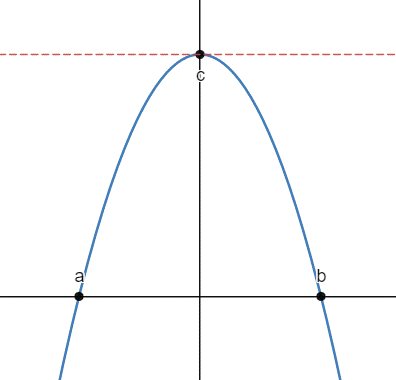
\includegraphics[scale=0.6]{DifferentialCalculusPictures/RollesTheorem.png}}

Intermediate Value Theorem:\\
If $f(x)$ is continuous on $[a,b]$ then there exists some real number $f(c)$ between $f(a)$ and $f(b)$ such that $a<c<b$\\
Ex: Show that there exists a positive real number $0<x<\frac{\pi}{2}$ for which $\cos(2x)=\sin x$
\begin{align*}
    &f(x)=\cos 2x-\sin x\\
    &f(0)=1\\
    &f\brround{\frac{\pi}{2}}=-2
\end{align*}
By the IVT, this guarantees that $f(x)$ must have at least one solution because the function must cross the x-axis.\\
Ex2: Find a solution to $f(x)=x^5-2x^4+2$
\begin{align*}
    &\lim_{x\to\infty}f(x)=\infty\text{ and }\lim_{x\to-\infty}f(x)=-\infty\therefore\text{ a solution exists}\\
    &f(-1)=-1,\,f(0)=2,\,f(1)=1
\end{align*}
By IVT, there is a zero between $-1$ and 0.\\
Using bisection, we can approximate the solution through multiple iterations.
\begin{align*}
    &-1<x<0\\
    &f\brround{-\frac{1}{2}}>0\therefore\,-1<x<-\frac{1}{2}\\
    &f\brround{-\frac{3}{4}}>0\therefore\,-1<x<-\frac{3}{4}\\
    &\vdots\\
    &-0.9104728699\ldots<x<-0.9104719162\ldots
\end{align*}
\\
Mean Value Theorem:\\
Rolle's Theorem is a generalization of the Mean Value Theorem (MVT). The MVT states that if $y=f(x)$ is a continuous function over $[a,b]$ and is differentiable on $(a,b)$ then there is at least one number $c$ between $a$ and $b$ such that:
$$\frac{f(b)-f(a)}{b-a}=f'(c)$$
Essentially, if you take the average between two points, a continuous function must attain that average value at least once.\\
\centerline{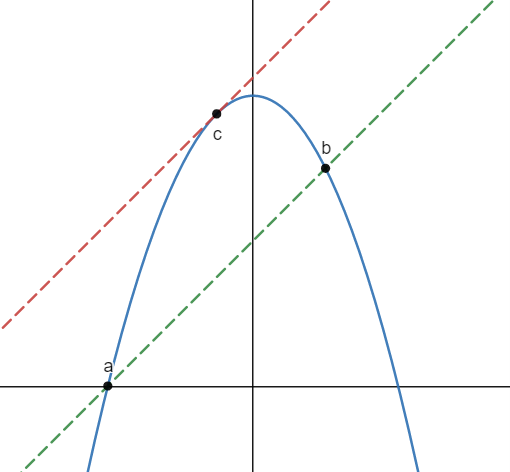
\includegraphics[scale=0.6]{DifferentialCalculusPictures/MVTImage.png}}
Ex: for the function $\frac{1}{x}$ over $[1,3]$ find all values $c$ that satisfy the mean value theorem.
\begin{align*}
    &f(x)=\frac{1}{x}\\
    &f'(x)=-\frac{1}{x^2}\\
    &f'(c)=\frac{f(3)-f(1)}{3-1}\\
    &-\frac{1}{c^2}=\frac{\frac{1}{3}-1}{2}=\frac{-\frac{2}{3}}{2}=-\frac{1}{3}\\
    &\Ra c^2=3\\
    &c=\pm\sqrt{3}\\
    &\text{Check domain } c\in(1,3)\\
    &c=\sqrt{3}
\end{align*}
Ex2: Show that for $0<x<\frac{\pi}{2}$, $\tan x<x$
\begin{align*}
    &f(x)=\tan x,\,f'(x)=\sec^2x\\
    &\frac{f(x)-f(a)}{x-a}=f'(c)\Ra f(x)=f(a)+f'(c)(x-a)\\
    &\text{set }a=0\\
    &f(x)=\tan x=\sec^2c\cdot x\\
    &\text{recall }0<c<\frac{\pi}{2}\therefore \sec c>0\\
    &\Ra\tan x=\sec^2c\cdot x>x\\
    &\therefore\tan x>x
\end{align*}
Ex3: Suppose $1\leq f'(t)\leq 5$ for all $t$ and $f(0)=0$. What are possible values of $t$ for which $f(t)=3000$?
\begin{align*}
    &\frac{f(t)-0}{t-0}=\frac{3000}{t}=f'(c)\text{ for }1\leq f'(c)\leq 5\\
    &1\leq\frac{3000}{t}\leq 5\\
    &\frac{1}{5}\leq\frac{t}{3000}\leq 1\\
    &600\leq t\leq 3000
\end{align*}
Ex4: Show that $|\sin x-\sin y|\leq |x-y|$ for all $x,y$
\begin{align*}
    &f(t)=\sin t,\,f'(t)=\cos t\\
    &\frac{\sin x-\sin y}{x-y}=\cos c\\
    &\left|\frac{\sin x-\sin y}{x-y}\right|=|\cos c|\leq 1\\
    &\therefore\,|\sin x-\sin y|\leq |x-y|
\end{align*}

\subsubsection{L'H\^opital's Rule}
L'H\^opital's Rule states that: Provided the limit exists, if $f(x_0)=g(x_0)=0$ then:
$$\lim_{x\to x_0}\frac{f(x)}{g(x)}=\lim_{x\to x_0}\frac{f'(x)}{g'(x)}$$
This allows us to calculate limits with indeterminate forms such as $\frac{0}{0}$.\\
Indeterminate forms can be any of the following:
\begin{align*}
    &\frac{0}{0}\\
    &\frac{\infty}{\infty}\\
    &0\cdot\infty\\
    &0^0\\
    &\infty^0\\
    &1^\infty\\
    &\infty-\infty
\end{align*}
\begin{align*}
    \text{Ex: }&\lim_{x\to 1}\frac{x^3-x^2-x+1}{x^3-2x^2+1}\\
    &=\lim_{x\to 1}\frac{3x^2-2x-1}{3x^2-4x+1}=\frac{0}{0}\\
    &=\lim_{x\to 1}\frac{6x-2}{6x-4}\\
    &=2
\end{align*}
Solving for $\frac{0}{0}$ and $\frac{\infty}{\infty}$ is easy as they are already in fraction form. The other indeterminate forms are trickier to solve.\\
For $0\cdot\infty$ we can rewrite it in the form of
    $$\lim_{x\to a}f(x)g(x)=\lim_{x\to a}\frac{f(x)}{1/g(x)}$$
\begin{align*}
    \text{Ex: }&\lim_{x\to 0^+}x^2\ln x\\
    &=\lim_{x\to 0^+}\frac{\ln x}{1/x^2}=\frac{-\infty}{\infty}\\
    &=\lim_{x\to 0^+}\frac{1/x}{-2/x^3}=-\frac{1}{2}\lim_{x\to 0^+}x^2\\
    &=0
\end{align*}
For any limits with exponentials we can take the log of both sides and solve for the log of the limit and then exponentiate to get the limit.
\begin{align*}
    \lim_{x\to a}f(x)^{g(x)}\\
    \Ra\lim_{x\to a}g(x)\ln(f(x))=L\\
    \lim_{x\to a}f(x)^{g(x)}=e^L
\end{align*}
\begin{align*}
    \text{Ex: }&\lim_{x\to 0^+}\brround{\frac{1}{\sin x}}^{\sin x}\\
    &\lim_{x\to 0^+}-\sin x\ln(\sin x)=L\\
    &L=\lim_{x\to 0^+}\frac{\ln(\sin x)}{1/\sin x}=\lim_{x\to 0^+}\frac{\ln(\sin x)}{\csc x}\\
    &L=\lim_{x\to 0^+}\frac{\frac{\cos x}{\sin x}}{-\csc x\cot x}=\lim_{x\to 0^+}\brround{-\sin x}=0\\
    &\therefore \lim_{x\to 0^+}\brround{\frac{1}{\sin x}}^{\sin x}=e^0=1
\end{align*}
\begin{align*}
    \text{Ex2: }&\lim_{x\to \infty}\brround{1+\frac{a}{x}}^{bx}\\
    &L=\lim_{x\to \infty}bx\ln\brround{1+\frac{a}{x}}=\lim_{x\to \infty}\frac{b\ln\brround{1+\frac{1}{a}}}{1/x}=\lim_{x\to \infty}\frac{b\brround{\frac{1}{1+\frac{a}{x}}}\brround{\frac{-a}{x^2}}}{\frac{-1}{x^2}}\\
    &=\lim_{x\to \infty}\frac{ab}{1+\frac{a}{x}}=ab\\
    &\therefore \lim_{x\to \infty}\brround{1+\frac{a}{x}}^{bx}=e^{ab}
\end{align*}

\subsubsection{Curve Sketching}
The derivative of a function is a powerful tool in being able to graph it.\\
First Derivative Test:
\begin{itemize}
    \item If $f'(x)>0$ over $(a,b)$ then $f(x)$ is increasing on $[a,b]$
    \item If $f'(x)<0$ over $(a,b)$ then $f(x)$ is decreasing on $[a,b]$
    \item If $f'(x)=0$ then $f(x)$ will have a local max/min
\end{itemize}
To see what the curve of the graph looks like we can use the concavity:\\
\centerline{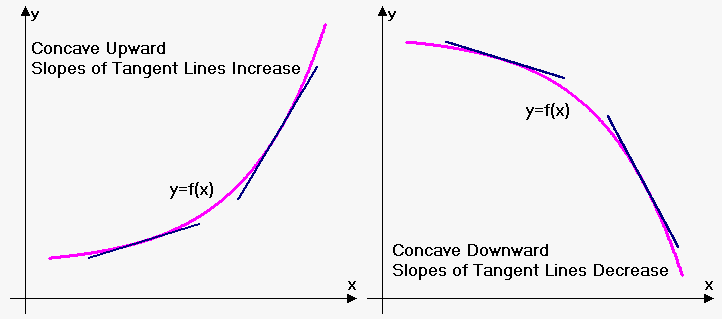
\includegraphics[scale=0.7]{DifferentialCalculusPictures/Concavity.png}}
The point where a curve changes concavity is called an inflection point.\\
Second Derivative Test:
\begin{itemize}
    \item If $f''(x)>0$ over $(a,b)$ then $f(x)$ is concave up.
    \item If $f''(x)<0$ over $(a,b)$ then $f(x)$ is concave down.
    \item If $f''(x)=0$ then $f(x)$ will have an inflection point.
\end{itemize}
Many functions can be simplified by exposing some symmetry:
\begin{description}
    \item[Even Function:] A function is even if $f(-x)=f(x)$.\\
    This means that all points are reflected across the y-axis.\\
    Ex: $y=\cos x$ or $y=x^2$
    \item[Odd Function:] A function is odd if $f(-x)=-f(x)$\\
    This means that the function is symmetric across the origin.\\
    Ex: $y=\sin x$ or $y=x^3$
\end{description}
The last thing yet to consider is what happens at the end points and asymptotes of a function.\\
We want to take the limit of the function at $\pm\infty$ and any points where the function is undefined to find any potential asymptotes.\\
Oblique asymptotes may occur in rational functions where the degree of the numerator is one higher than the degree in the denominator.
\begin{align*}
    \text{Ex: }&y=\dfrac{x^2-16}{x-7}\\
    &\text{by long division }\frac{x^2-16}{x-7}=x+7+\frac{33}{x-7}
\end{align*}
As $|x|$ gets very large, the $\dfrac{33}{x-7}$ term tends to 0 so $f(x)$ approaches the function $y=x+7$ as $|x|$ gets very large.\\
Put all together, we can follow a general procedure to sketch curves.
\begin{enumerate}
    \item Identify the base function and expected behavior
    \item Find the domain (and range) of the function and any non permissible values
    \item Identify any symmetry
    \item Plot any known intercepts
    \item Find all asymptotes and end behavior
    \item Find critical points
    \item First derivative test
    \item Find inflection points
    \item Second derivative test
\end{enumerate}
Ex: $y=\dfrac{x}{\ln x}$\\
Domain: $x>0$\\
NPVs: $x\neq 0$, $x\neq 1$\\
Symmetry: none\\
Intercepts: none\\
Asymptotes and boundaries:
\begin{align*}
    &\lim_{x\to 0^+}\frac{x}{\ln x}=\frac{0}{-\infty}=0\\
    &\lim_{x\to 1^-}=\frac{1}{0^-}=-\infty\\
    &\lim_{x\to 1^+}=\frac{1}{0^+}=\infty\\
    &\lim_{x\to \infty}=\infty
\end{align*}
Critical Points:
\begin{align*}
    &f'(x)=\frac{\ln x-x\brround{\frac{1}{x}}}{(\ln x)^2}=\frac{\ln x-1}{(\ln x)^2}\\
    &f'(x)=0\Ra \ln x=1\\
    &x=e\\
    &f(e)=e\\
    &\rightarrow (e,e)
\end{align*}
First Derivative Test:\\
\begin{tabular}{c||c|c}
    Interval & $f'(x)$ & $f(x)$\\
    \hline
    $0<x<1$ & $-$ & decreasing\\
    $1<x<e$ & $-$ & decreasing\\
    $x>e$ & $+$ & increasing
\end{tabular}\\
Inflection Points:
\begin{align*}
    &f''(x)=\frac{2-\ln x}{x(\ln x)^3}\\
    &f''(x)=0\Ra \ln x=2\\
    &x=e^2\\
    &f(e^2)=\frac{e^2}{2}\\
    &\rightarrow \brround{e^2,\frac{e^2}{2}}
\end{align*}
Second Derivative Test:\\
\begin{tabular}{c||c|c}
    Interval & $f''(x)$ & $f(x)$\\
    \hline
    $0<x<1$ & $-$ & concave down\\
    $1<x<e^2$ & $+$ & concave up\\
    $x>e^2$ & $-$ & concave down
\end{tabular}\\
\\
\centerline{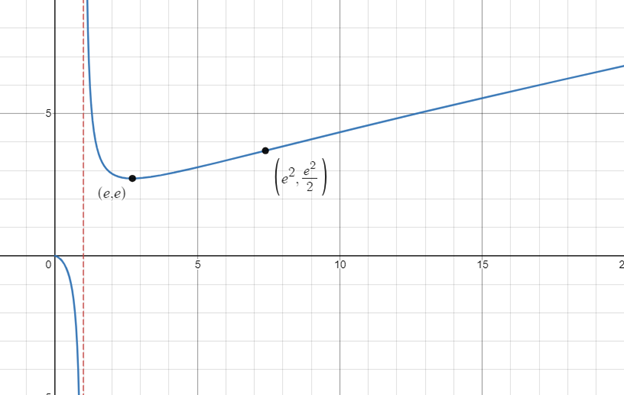
\includegraphics[scale=0.9]{DifferentialCalculusPictures/SketchingEx1.png}}







\subsection{Applications of Derivatives}

\subsubsection{Optimization}
Optimization uses maxima and minima to identify optimal solutions to problems given a restraint and equation.\\
Steps to solve:
\begin{enumerate}
    \item Define the relevant quantities
    \item Determine a formula in the form $f(x)$
    \item Find an interval of possible values from physical restrictions
    \item Take the derivative and find critical points
    \item Find the maximum/minimum values
\end{enumerate}
Ex: A rectangular enclosure is to be built with one side against a wall and 3 sides fenced. 100m of fence is available. What is the maximum possible area?
\begin{align*}
    &A=lw\\
    &P=100=2w+l\\
    &\Ra l=100-2w\\
    &A(w)=x(100-2x)=100-2x^2\\
    &\text{Restrictions: }w\geq 0,\, l\geq 0\Ra 100-2w\geq 0\Ra 0\leq w\leq 50\\
    &\frac{dA}{dw}=100-4w=0\Ra w=25\\
    &\text{Test critical points: }\\
    &A(0)=0\\
    &A(25)=1250\\
    &A(50)=0\\
    &\therefore \text{max area is }1250m^2
\end{align*}
Ex2: An IMAX movie screen is 16m tall, base 9m above eye level. How far from the screen is the "best" view? (goal: maximize $\theta$)\\
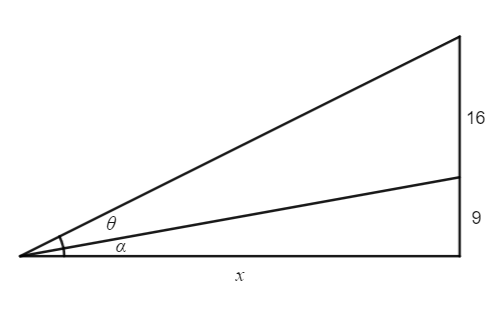
\includegraphics[scale=0.8]{DifferentialCalculusPictures/OptimizationEx.png}
\begin{align*}
    &\tan\alpha=\frac{9}{x}
    &\tan(\alpha+\theta)=\frac{25}{x}\\
    &\alpha=\arctan\brround{\frac{9}{x}}
    &\alpha+\theta=\arctan\brround{\frac{25}{x}}\\
    &\theta=\arctan\brround{\frac{25}{x}}-\arctan\brround{\frac{9}{x}}\\
    &\text{endpoints:}\\
    &\lim_{x\to0^+}\theta=\frac{\pi}{2}-\frac{\pi}{2}=0\\
    &\lim_{x\to\infty}\theta=0\\
    &\text{critical points:}\\
    &\theta'(x)=\frac{16(15^2-x^2)}{(x^2+9^2)(x^2+25^2)}\\
    &\Ra x=15
\end{align*}
Ex3: Find the volume of the largest cylinder that can be inscribed in a cone.\\
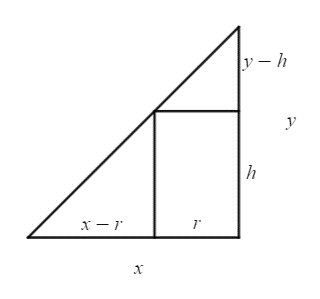
\includegraphics[scale=0.65]{DifferentialCalculusPictures/InscribedCylinder.png}
\begin{align*}
    &V=\pi r^2 h\\
    &\text{Using like triangles: }\frac{h}{x-r}=\frac{y}{x}\\
    &h=\frac{y(x-r)}{x}\\
    &V=\pi r^2\frac{y}{x}(x-r)=\pi r^2y-\pi r^3\frac{y}{x}\\
    &\text{*treat $x$ and $y$ as constants*}\\
    &2\pi ry-3\pi r^2\frac{y}{x}\\
    &\frac{dV}{dr}=2\pi ry\brround{2-\frac{3r}{x}}=0\Ra r=0,\,r=\frac{2x}{3}\\
    &h=\frac{y\brround{x-\frac{2x}{3}}}{x}=\frac{y}{3}\\
    &V=\pi\brround{\frac{2x}{3}}^2\brround{\frac{y}{3}}=\frac{4\pi}{27}x^2y
\end{align*}
We can also calculate the ratio of the two volumes to find that the volume of the cylinder is $\frac{4}{9}$ the volume of the cone.
\begin{align*}
    \frac{V_{cylinder}}{V_{cone}}=\frac{\frac{4\pi}{27}x^2y}{\frac{\pi}{3} x^2y}=\frac{4}{9}
\end{align*}
Ex4: Of all tangent lines to $y=\dfrac{6}{x^2+3}$, which have maximum slope?
\begin{align*}
    &S=\frac{dy}{dx}=\frac{-12x}{(x^2+3)^2}\\
    &\frac{dS}{dx}=36\brround{\frac{x^2-1}{(x^2+3)^3}}\\
    &\lim_{x\to\pm\infty}S=0\\
    &\Ra S(-1)=\frac{3}{4},\, S(1)=-\frac{3}{4}\\
    &\therefore\text{ max is at }x=-1
\end{align*}

\subsubsection{Related Rates}
Related rates compares how changing one variable with respect to time affects the rate of change of another related variable.\\
Ex: A 25 foot ladder is leaning against a wall and is sliding down towards the ground. If the foot of the ladder is sliding away from the wall at 15ft/s, how fast is the top of the ladder sliding down the wall when the top of the ladder is 7 feet from the ground?\\
Let $y$ be the vertical distance and $x$ be the horizontal distance.\\
\begin{align*}
    &x^2+y^2=25^2=625\\
    &2x\frac{dx}{dt}+2y\frac{dy}{dt}=0\\
    &\frac{dy}{dt}=-\frac{x}{y}\frac{dx}{dt}\\
    &\text{for $y=7$, }x^2+49=625\Ra x=24\\
    &\frac{dy}{dt}=-\frac{24}{7}(15)=-\frac{360}{7}\mathrm{ft/s}
\end{align*}
Ex2: An underground conical tank with its vertex down is filled with water at a rate of $18\pi$ft$^3$/min. If the tank has a height of 30ft and radius 15 feet, how fast is the water rising. when the water is 12 feet deep?\\
Let $h$ be the current height of the cone and $r$ be the current radius.
\begin{align*}
    &V=\frac{1}{3}\pi r^2h\\
    &\frac{r}{h}=\frac{15}{30}\Ra r=\frac{h}{2}\\
    &V=\frac{\pi}{3}\brround{\frac{h}{2}}^2h=\frac{\pi}{12}h^3\\
    &\frac{dV}{dt}=\frac{\pi}{4}h^2\frac{dh}{dt}\\
    &\frac{dh}{dt}=\frac{4}{\pi h^2}\frac{dV}{dt}=\frac{4}{\pi(12)^2}(18\pi)=\frac{1}{2}\mathrm{ft/min}
\end{align*}




















































% Integral calculus



\section{Integral Calculus}
\subsection{Definition of the Integral}
\subsubsection{Antidifferentiation}
The antiderivative is the reverse of the derivative and is found by integration. When we integrate, we must include an arbitrary constant $C$, in order to include every possible antiderivative in our solution. This is because the derivative of a constant is always 0.
$$\int f(x)dx=F(x)+C$$
Many of the elementary functions have antiderivatives that are relatively simple to compute:
\begin{align*}
    &\int x^ndx=\frac{x^{n+1}}{n+1}+C\\
    &\int \frac{dx}{x}=\ln|x|+C\\
    &\int \sin{x} dx=-\cos x+C\\
    &\int \cos{x} dx=\sin x+C\\
    &\int e^xdx=e^x+C
\end{align*}
Ex: $\int xdx=\frac{1}{2}x^2+C$\\
\subsubsection{Numeric Integration}
Riemann Sums:
The integral of a function is analogous to the area under the curve. This can be shown using Riemann Sums.\\
We can express the area under a curve by breaking up the area into a series of rectangles.\\
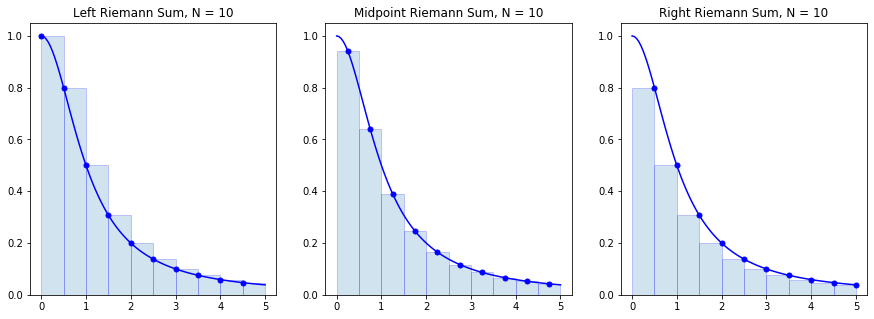
\includegraphics[scale=0.57]{IntegralCalcPictures/RiemannSums.png}\\
For the area under the curve $y=x$ between 0 and 1, if we break it up into 4 sections, the width of each rectangle will be $\frac{1}{4}$. The height of the rectangles will depend on whether you take left, right, or mid endpoints. Taking left endpoints, the heights will be $0,\,\frac{1}{4},\,\frac{1}{2},\,\frac{3}{4}$. So the total area is the sum of the 4 rectangles, $A=0+\frac{1}{16}+\frac{1}{8}+\frac{3}{16}=\frac{3}{8}$ which is close to the actual value of $\frac{1}{2}$.\\
In general, the area under a curve can be expressed as
$$A\approx\sum_{i=1}^nf(x_i^*)\Delta x$$
$\Delta x$ is the width of the rectangles. where 
\begin{align*}
    &\Delta x =\frac{b-a}{n}
\end{align*}
and $x_i^*$ refers to the position of the rectangle and the end points.
\begin{align*}
    \text{Right: }&x_i^*=a+i\Delta x\\
    \text{Left: }&x_i^*=a+(i-1)\Delta x\\
    \text{Mid: }&x_i^*=a+\brround{i-\frac{1}{2}}\Delta x
\end{align*}
The more rectangles we use, the better the approximation. As we take the limit as $n\to\infty$, we will get an exact value for the area.
Ex: Area of $y=x$ between 0 and 1.
\begin{align*}
    &A=\lim_{n\to\infty}\sum_{i=1}^nf(x_i^*)\Delta x\\
    &\Delta x=\frac{1-0}{n}\\
    &x_i^*=i\Delta x=\frac{i}{n}\\
    &A=\lim_{n\to\infty}\sum_{i=1}^n\frac{i}{n^2}=\lim_{n\to\infty}\frac{1}{n^2}\sum_{i=1}^ni\\
\end{align*}
We have the following formulas in order to express sums
\begin{align*}
    \sum_{i=1}^n1&=n\\
    \sum_{i=1}^ni&=\frac{n(n+1)}{2}\\
    \sum_{i=1}^ni^2&=\frac{n(n+1)(2n+1)}{6}\\
    \sum_{i=1}^ni^3&=\frac{n^2(n+1)^2}{4}
\end{align*}
So we can express the area in our example as
\begin{align*}
    A&=\lim_{n\to\infty}\frac{1}{n^2}\sum_{i=1}^ni=\lim_{n\to\infty}\frac{n(n+1)}{2n^2}=\lim_{n\to\infty}\frac{n^2}{2n^2}+\frac{n}{2n^2}=\frac{1}{2}+\lim_{n\to\infty}\frac{1}{2n}\\
    &=\frac{1}{2}
\end{align*}
which fits with what we expect\\
An important thing to note is that the area under a curve can come out negative if the function is below the x-axis.\\
Ex2: Find the area under the curve $f(t)=t^2$ between 0 and some number $x$.
\begin{align*}
    &\Delta t=\frac{x}{n}\\
    &x_i^*=\frac{ix}{n}\\
    &A=\lim_{n\to\infty}\sum_{i=1}^n\frac{i^2x^3}{n^3}=\lim_{n\to\infty}\frac{x^3}{n^3}\sum_{i=1}^ni^2\\
    &A=\lim_{n\to\infty}\frac{x^3}{n^3}\cdot\frac{n(n+1)(2n+1)}{6}\\
    &A=\lim_{n\to\infty}\frac{x^3}{3}+\frac{1}{2n}+\frac{1}{6n^2}=\frac{x^3}{3}
\end{align*}
Notice this is the same as the antiderivative $\int x^2dx=\frac{x^3}{3}$ so we can see that the integral is analogous to the area under the curve.\\

Another method of numeric integration is the trapezoidal method where instead of using rectangles, we use trapezoids to form the area.
$$\Delta A=\Delta x\brround{\frac{y_0+y_1}{2}}$$
This happens to be identical to taking midpoints using Riemann sums.\\
A better method of numerical integration is Simpson's Rule:\\
This involves using the area under a parabola as a basis for approximation.
$$\Delta A=2\Delta x\brround{\frac{y_0+4y_1+y_2}{6}}$$
Where $2\Delta x$ is the base and $\dfrac{y_0+4y_1+y_2}{6}$ is the average height of the parabola. This works out to be
$$A=\frac{\Delta x}{3}(y_0+4y_1+2y_2+4y_3+\cdots+2y_{n-2}+4y_{n-1}+y_n)$$
Note that for Simpson's rule, we require that $n$ be an even number.\\
Ex: Estimate $\int_0^\pi\sin xdx$ using $n=4$\\
\begin{tabular}{c|c|c}
    $i$ & $x_i$ & $f(x_i)$\\
    \hline
    0 & 0 & 0\\
    1 & $\frac{\pi}{4}$ & $\frac{\sqrt{2}}{2}$\\
    2 & $\frac{\pi}{2}$ & 1\\
    3 & $\frac{3\pi}{4}$ & $\frac{\sqrt{2}}{2}$\\
    4 & $\pi$ & 0
\end{tabular}\\
\begin{align*}
    A=&\frac{\Delta x}{3}(y_0+4y_1+2y_2+4y_3+y_4)\\
    &=\frac{\pi}{12}(0+2\sqrt{2}+2+2\sqrt{2}+0)=\frac{\pi}{6}(1+2\sqrt{2})
\end{align*}
\subsubsection{The Definite Integral}
We can define the definite integral as the infinite sum of the area and can be written as
$$\int_a^bf(x)dx=\lim_{n\to\infty}\sum_{i=1}^nf(x_i^*)\Delta x$$
We can convert infinite sums to integral form by identifying the bounds and the function. Some things to look for are:
\begin{itemize}
    \item look for $\frac{i^*}{n}$ combos to spot $x_i$
    \item look for an additional $\frac{1}{n}$ term on the outside of the function to spot $\Delta x$
\end{itemize}
\begin{align*}
    \text{Ex: }&\lim_{n\to\infty}\sum_{i=1}^n\frac{\sqrt{i^2+9n^2}}{i^2}\\
    &I=\lim_{n\to\infty}\sum_{i=1}^n\sqrt{\frac{1}{i^2}+\frac{9n^2}{i^4}}\\
    &I=\lim_{n\to\infty}\sum_{i=1}^n\frac{1}{n}\sqrt{\frac{n^2}{i^2}+\frac{9n^4}{i^4}}\\
    &\text{assume }\Delta x=\frac{1}{n},\,x_i^*=\frac{i}{n}\\
    &I=\int_0^1\sqrt{\frac{1}{x^2}+\frac{9}{x^4}}dx=\int_0^1\frac{\sqrt{x^2+9}}{x^2}dx
\end{align*}
Note for these problems there are multiple different solutions. i.e. choosing left-hand end points vs. right-hand end points will give different answers.\\

Integral Properties:\\
Integrals have all the usual addition/subtraction properties as well as some other useful identities:
\begin{align*}
    &\int_a^af(x)dx=0\\
    &\int_a^bf(x)dx=-\int_b^af(x)dx\\
    &\int_a^bf(x)dx=\int_a^cf(x)dx+\int_c^bf(x)dx\\
    &\text{if $f(x)$ is even, }\int_{-a}^af(x)dx=2\int_0^af(x)dx\\
    &\text{if $f(x)$ is odd, }\int_{-a}^af(x)dx=0
\end{align*}

Fundamental Theorem of Calculus 1:
We have seen how the area under a curve is related to the antiderivative of the curve. This is expressed in the FTC1
$$\int_a^b f(x)dx=F(b)-F(a)=\left.F(x)\right|^b_a=\brsquare{F(x)}^b_a$$
\begin{align*}
    \text{Ex: }\int_0^12xdx=\left.x^2\right|_0^1=1^2-0^2=1
\end{align*}
In some situations, you may be required to break the function into separate integrals in order to evaluate them.
\begin{align*}
    \text{Ex2: }&\int_{-2}^1|2x-1|dx\\
    &I=\int_{-2}^{\frac{1}{2}}(1-2x)dx+\int_{\frac{1}{2}}^1(2x-1)dx\\
    &I=\brsquare{x-x^2}_{-2}^{1/2}+\brsquare{x^2-x}_{1/2}^1=6.5
\end{align*}

\subsubsection{Transcendental Functions}
We have seen transcendental numbers such as $\pi$ or $\sqrt{2}$. They are numbers that are described in terms of themselves and cannot be expressed in terms of what we already know. This same thing can be done with functions. $\sin x$ and $\ln x$ are examples of transcendental functions. With the Second Fundamental Theorem of Calculus, we are able to create more transcendental functions.\\
The 2nd Fundamental Theorem (FTC2) is known as
$$f(x)=\frac{d}{dx}\int_a^xf(t)dt$$
We can express the derivatives of these functions using the FTC1 and chain rule:\\
\begin{align*}
    F(x)=\displaystyle{\int^{u(x)}_{v(x)}f(x)dx}=F(u)-F(v)\\
    F'(x)=f(u)u'-f(v)v'
\end{align*}
\begin{align*}
    \text{Ex: }&\frac{d}{dx}\int_x^{x^2}\cos t dt=2x\cos x^2-\cos x
\end{align*}
While we always know the derivative of an integral, not all integrals themselves are solvable. The ones that aren't solvable are where we can come up with transcendental functions and we can use the information from its derivative to figure out what it may look like
\begin{align*}
    \text{Ex: }&f(x)=\int_1^x\frac{dt}{t}\\
    &f(1)=\int_1^1\frac{dt}{t}=0\\
    &f'(x)=\frac{1}{x}\Ra\text{increasing for }x>0\\
    &f''(x)=-\frac{1}{x^2}\Ra\text{concave up for all }x
\end{align*}
This function, you may recognize, is the definition of $\ln x$
\begin{align*}
    \text{Ex2: }&f(x)=\int_0^xe^{-t^2}dt\\
    &f(0)=0\\
    &f'(x)=e^{-x^2}\Ra\text{always increasing}\\
    &f'(0)=1\\
    &\lim_{x\to\pm\infty}f'(x)=0\therefore\,f(x)\text{ has asymptotes at }\pm\infty\\
    &f''(x)=-2xe^{-2x^2}\Ra\text{concave up for }x<0,\text{ concave down for }x>0
\end{align*}
\centerline{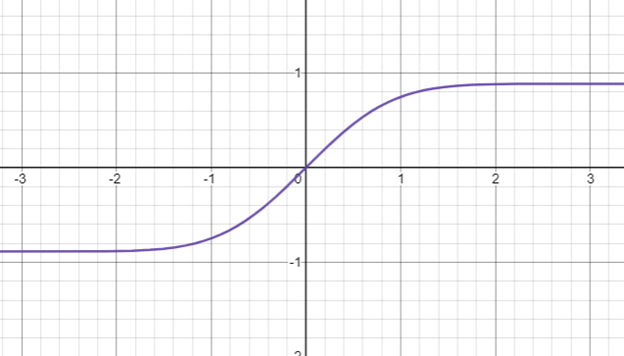
\includegraphics[scale=0.8]{IntegralCalcPictures/AreaOfBellCurve.png}}
This function is the area of the bell curve. The error function $\erf x$, is based on this and is defined as
$$\erf x=\frac{2}{\sqrt{\pi}}\int_0^xe^{-t^2}dt$$
Some other notable functions include:
\begin{align*}
    &\mathrm{C}(x)=\int_0^x\cos(t^2)dt\\
    &\mathrm{S}(x)=\int_0^x\sin(t^2)dt\\
    &\mathrm{H}(x)=\int_0^x\frac{\sin t}{t}dt\\
    &\mathrm{Li}(x)=\int_2^x\frac{dt}{\ln t}\\
    &\Gamma(x)=\int_0^xe^{-t}t^{x-1}dt
\end{align*}
Where $\mathrm{Li}(x)$ is approximately the number of primes less than $x$.\\
and $\Gamma(x)$ is the same as $(x-1)!$












\subsection{Integration Techniques}
\subsubsection{Substitution}
Substitution is used to help solve messy integrals and is a very common tool. It is the opposite to the chain rule. We can choose an expression of $x$ to replace with $u$. Note that this will also change the differential and the bounds of integration.
\begin{align*}
    \text{Ex: }&\int (x+2)^{10}dx\\
    &\text{let }u=x+2\Ra du=dx\\
    &\int u^{10}du=\frac{u^{11}}{11}+C\\
    &=\frac{(x+2)^{11}}{11}+C
\end{align*}
\begin{align*}
    \text{Ex2: }&\int(5x^2+1)\sqrt{5x^3+3x-2}dx\\
    &\text{let }u=5x^3+3x-2\\
    &du=(15x^2+3)dx\Ra\frac{du}{3}=(5x^2+1)dx\\
    &\int \frac{1}{3}\sqrt{u}du=\frac{1}{3}\frac{u^{3/2}}{3/2}+C=\frac{2u^{3/2}}{9}+C\\
    &=\frac{2}{9}(5x^3+3x-2)^{3/2}+C
\end{align*}
\begin{align*}
    \text{Ex3: }&\int \frac{\sin x}{(2+\cos x)^2}dx\\
    &\text{let }u=2+\cos x\\
    &du=-\sin x dx\Ra-du=\sin x dx\\
    &\int\frac{-du}{u^2}=\frac{1}{u}+C\\
    &=\frac{1}{2+\cos x}+C
\end{align*}
\begin{align*}
    \text{Ex4: }&\int\frac{\ln x}{x}dx\\
    &\text{let }u=\ln x\Ra du=\frac{dx}{x}\\
    &\int udu=\frac{u^2}{2}\\
    &=\frac{(\ln x)^2}{2}+C
\end{align*}
\begin{align*}
    \text{Ex5: }&\int a^xdx\\
    &a^x=e^{\ln a^x}=e^{x\ln a}\\
    &\text{let }u=x\ln a\Ra du=\ln a\\
    &\int \frac{e^{u}}{\ln a}du=\frac{e^u}{\ln a}+C=\frac{e^{x\ln a}}{\ln a}+C\\
    &=\frac{a^x}{\ln a}+C
\end{align*}
\begin{align*}
    \text{Ex6: }&\int\tan xdx\\
    &I=\int\frac{\sin x}{\cos x}dx\\
    &\text{let }u=\cos x\Ra du=-\sin xdx\Ra -du=\sin xdx\\
    &I=-\int\frac{du}{u}=-\ln|u|+C\\
    &=-\ln|\cos x|+C
\end{align*}
Note that when we use substitution with a definite integral, the bounds change.
\begin{align*}
    \text{Ex7: }&\int_0^1\frac{3x}{(x^2+1)^2}dx\\
    &\text{let }u=x^2+1\Ra du=2xdx\Ra \frac{3}{2}du=3dx\\
    &u(0)=1,\,u(1)=2\\
    &I=\frac{3}{2}\int_1^2\frac{du}{u^2}=\frac{3}{2}\brsquare{-\frac{1}{u}}^2_1\\
    &=\frac{3}{4}
\end{align*}
\subsubsection{Integration by Parts}
Integration by parts is the opposite of the product rule.
\begin{align*}
    &d(uv)=udv+vdu\\
    &udv=d(uv)-vdu\\
    &\int udv=uv-\int vdu
\end{align*}
Using the derived formula, we can decompose the integral of a product in the following way.\\
Typically, we take $u$ to be a function easy to differentiate and $dv$ to be a function easy to integrate.
\begin{align*}
    \text{Ex: }&\int x\sin xdx\\
    &\text{let }u=x\Ra du=dx\\
    &\text{let }dv=\sin xdx\Ra v=-\cos x\text{*}\\
    &\int x\sin xdx=-x\cos x+\int \cos xdx\\
    &=-x\cos x+\sin x+C
\end{align*}
*Note we ignore the $+C$ when integrating $dv$ as we instead add it in later with the final solution.\\
Sometimes, we may have to complete integration by parts multiple times to get a solution.\\
Other times, we may never be able to solve explicitly but can come to an answer by recursion.
\begin{align*}
    \text{Ex2: }&I=\int e^{2x}\cos x dx\\
    &\text{let }u=e^{2x}\Ra du=2e^{2x}dx\\
    &\text{let }dv=\cos xdx\Ra v=\sin x\\
    &I=e^{2x}\sin x-\int \sin x2e^{2x}dx=e^{2x}\sin x-2\int e^{2x}\sin x dx\\
    &\text{solve }\int e^{2x}\sin xdx\\
    &\text{let }u=e^{2x}\Ra du=2e^{2x}dx\\
    &\text{let }dv=\sin xdx\Ra v=-\cos x\\
    &I=e^{2x}\sin x-2\brround{-e^{2x}\cos x-\int (-\cos x)(2e^{2x}dx)}\\
    &I=e^{2x}\sin x+2e^{2x}\cos x-4\int e^{2x}\cos xdx\\
    &\text{recall }I=\int e^{2x}\cos x dx\\
    &I=e^{2x}\sin x+2e^{2x}\cos x-4I\\
    &5I=e^{2x}\sin x+2e^{2x}\cos x\\
    &I=\frac{1}{5}\brround{e^{2x}\sin x+2e^{2x}\cos x}+C
\end{align*}
\begin{align*}
    \text{Ex3: }&\int \ln xdx\\
    &\text{let }u=\ln x\Ra du=\frac{dx}{x}\\
    &dv=dx\Ra v=x\\
    &I=x\ln x-\int \frac{x}{x}dx\\
    &=x\ln x-x+C
\end{align*}
\begin{align*}
    \text{Ex4: }&\int \arctan xdx\\
    &\text{let }u=\arctan x\Ra du=\frac{dx}{1+x^2}\\
    &dv=dx\Ra v=x\\
    &I=x\arctan x-\int\frac{x}{1+x^2}dx\\
    &\text{let }w=1+x^2\Ra dw=2dx\Ra \frac{dw}{2}=dx\\
    &I=x\arctan x-\frac{1}{2}\int\frac{dw}{w}=x\arctan x-\frac{1}{2}\ln w+C\\
    &=x\arctan x-\frac{1}{2}\ln(1+x^2)+C
\end{align*}
Ex5: Let $I_n=\int_0^{2\pi}\sin^n xdx$. Determine a recursive relation for $I_n$ and compute $\int_0^{2\pi}\sin^6xdx$
\begin{align*}
    &I_n=\int_0^{2\pi}\sin^{n-1}x\sin xdx\\
    &u=\sin^{n-1}x\Ra du=(n-1)\sin^{n-2}x\cos x dx\\
    &dv=\sin xdx\Ra v=-\cos x\\
    &I_n={-\sin^{n-1}x\cos x}\eval_0^{2\pi}+(n-1)\int_0^{2\pi}\sin^{n-2}x\cos^2xdx\\
    &I_n=0+(n-1)\int_0^{2\pi}(1-\sin^2x)\sin^{n-2}xdx\\
    &I_n=(n-1)\int_0^{2\pi}\sin^{n-2}xdx-(n-1)\int_0^{2\pi}\sin^nxdx\\
    &I_n=(n-1)I_{n-2}-(n-1)I_n\\
    &I_n=\frac{n-1}{n}I_{n-2}\\
    &\text{So, }\int_0^{2\pi}\sin^6xdx=I_6=\frac{5}{6}I_4=\frac{5}{6}\cdot\frac{3}{4}I_2=\frac{5}{6}\cdot \frac{3}{4}\cdot\frac{1}{2}I_0\\
    &I_0=\int_0^{2\pi}dx=2\pi\\
    &\therefore I_6=\frac{5\pi}{8}
\end{align*}
\subsubsection{Trigonometric Integrals}
Integrals of products of sines and cosines:\\
$\int\sin^ax\cos^bxdx$ where $a$ and $b$ are intigers.\\
Case when $a$ is odd:
\begin{align*}
    &\int\sin^ax\cos^bxdx=\int\sin^{a-1}x\cos^bx\sin xdx=\int(1-\cos^2x)^{\frac{a-1}{2}}\cos^bx\sin xdx\\
    &u=\cos x\Ra -du=\sin xdx\\
    &I=-\int u^b(1-u^2)^{\frac{a-1}{2}}du
\end{align*}
\begin{align*}
    \text{Ex: }&\sin^3x\cos^3xdx\\
    &\int(1-\cos^2x)\cos^3x\sin xdx\\
    &u=\cos x\Ra -du=\sin x\\
    &I=-\int(1-u^2)u^3du=-\int(u^3-u^5)du\\
    &I=\frac{u^6}{6}-\frac{u^4}{4}+C\\
    &=\frac{\cos^6x}{6}-\frac{\cos^4x}{4}+C
\end{align*}
Case when $b$ is odd:
\begin{align*}
    &\int sin^ax\cos^bxdx=\int\sin^ax\cos^{b-1}x\cos xdx=\int\sin^ax(1-\sin^2 x)^{\frac{b-1}{2}}\cos xdx\\
    &u=\sin x\Ra du=\cos xdx\\
    &I=\int u^a(1-u^2)^\frac{b-1}{2}du
\end{align*}
\begin{align*}
    \text{Ex: }&\int\sin^2x\cos^5xdx\\
    &I=\int\sin^2x(1-\sin^2x)^2\cos xdx\\
    &u=\sin x\Ra du=\cos xdx\\
    &I=\int u^2(1-u^2)^2du=\int(u^2-2u^4+u^6)du\\
    &I=\frac{u^3}{3}-\frac{2u^5}{5}+\frac{u^7}{7}+C\\
    &=\frac{\sin^3 x}{3}-\frac{2\sin^5x}{5}+\frac{\sin^7x}{7}+C
\end{align*}
Case when $a$ and $b$ are even:\\
In this case, we will require the following half-angle identities
\begin{align*}
    \cos(2\theta)&=\cos^2\theta-\sin^2\theta\\
    &=\cos^2\theta-(1-\cos^2\theta)\\
    &=2\cos^2\theta-1\\
    &\Ra\cos^2\theta=\frac{1+\cos(2\theta)}{2}
\end{align*}
We also have that
\begin{align*}
    \sin^2\theta=\frac{1-\cos(2\theta)}{2}\\
\end{align*}
The goal here is to express the integrand as a single trig term.
\begin{align*}
    \text{Ex: }&\int\sin^2(4x)\cos^2(4x)dx\\
    &I=\int(\sin(4x)\cos(4x))^2dx=\int\brround{\frac{\sin(8x)}{2}}^2dx=\frac{1}{4}\int\brround{\frac{1-\cos(16x)}{2}}dx\\
    &=\frac{1}{4}\brround{\frac{x}{2}-\frac{\sin(16x)}{32}}+C
\end{align*}
Integrals of products of tan and sec:\\
$\int\tan^ax\sec^bxdx$ where $a$ and $b$ are integers.\\
Case when $b$ is even:
\begin{align*}
    &\int\tan^ax\sec^bxdx=\int\tan^ax\sec^{b-2}x\sec^2xdx=\int\tan^ax(1+\tan^2x)^{\frac{b-2}{2}}\sec^2xdx\\
    &u=\tan x\Ra du=\sec^2xdx\\
    &I=u^a(1+u^2)^{\frac{b-2}{2}}du
\end{align*}
\begin{align*}
    \text{Ex: }&\int\tan^2x\sec^4xdx\\
    &I=\int\tan^2x\sec^2x\sec^2xdx=\int\tan^2x(1+\tan^2x)\sec^2xdx\\
    &u=\tan x\Ra du=\sec^2xdx\\
    &I=\int u^2(1+u^2)du\\
    &I=\frac{u^3}{3}+\frac{u^5}{5}+C\\
    &I=\frac{\tan^3x}{3}+\frac{\tan^5x}{5}+C
\end{align*}
Case when $a$ is odd and $b\geq 1$
\begin{align*}
    &\int\tan^ax\sec^bxdx=\tan^{a-1}\sec^{b-1}(\sec x\tan x)dx=\int(\sec^2x-1)^{\frac{a-1}{2}}\sec^{b-1}x(\sec x\tan x)dx\\
    &u=\sec x\Ra du=\sec x\tan xdx\\
    &I=(u^2-1)^{\frac{a-1}{2}}u^{b-1}du
\end{align*}
\begin{align*}
    \text{Ex: }&\int\tan^3x\sec^7xdx\\
    &I=\int\tan^2x\sec^6x(\sec x\tan x)dx=\int(\sec^2x-1)\sec^6x(\sec x\tan x)dx\\
    &u=\sec x\Ra du=\sec x\tan x dx\\
    &I=\int(u^2-1)u^6du=\frac{u^9}{9}-\frac{u^7}{7}+C\\
    &=\frac{\sec^9x}{9}-\frac{\sec^7x}{7}+C
\end{align*}
For other cases, there may not be any specific method.
\begin{align*}
    \text{Ex: }&\int\tan^4xdx\\
    &I=\int\tan^2x\tan^2xdx=\int\tan^2x(\sec^2x-1)dx\\
    &I=\int\tan^2x\sec^2xdx-\int\tan^2xdx\\
    &I=\int\tan^2x\sec^2xdx-\int(\sec^2x-1)dx\\
    &u=\tan x\Ra du=\sec^2xdx\\
    &I=\int u^2du-\int du+\int dx\\
    &I=\frac{u^3}{3}-u+x+C\\
    &=\frac{\tan^3x}{3}-\tan x+x+C
\end{align*}
\begin{align*}
    \text{Ex2: }&\int\sec xdx\\
    &I=\int\sec x\brround{\frac{\sec x+\tan x}{\sec x+\tan x}}dx=\int\frac{\sec^2x+\sec x\tan x}{\sec x+\tan x}dx\\
    &u=\sec x+\tan x\Ra du=(\sec x\tan x+\sec^2x)dx\\
    &I=\int\frac{du}{u}=\ln|u|+C\\
    &=\ln|\sec x+\tan x|+C
\end{align*}
\begin{align*}
    \text{Ex3: }&\int\sin(2x)\cos(3x)dx\\
    &\cos(3x)=\cos(2x+x)=\cos(2x)\cos x-\sin (2x)\sin x=4\cos^3x-3\cos x\\
    &\sin(2x)=2\sin x\cos x\\
    &I=\int(2\sin x\cos x)(4\cos^3x-3\cos x)dx\\
    &I=8\int\cos^4x\sin xdx-6\int\cos^2x\sin xdx\\
    &u=\cos x\Ra -du=\sin xdx\\
    &I=6\int u^2du-8\int u^4du=2u^3-\frac{8u^5}{5}+C\\
    &=-\frac{8}{5}\cos^5x+2\cos^3x+C
\end{align*}
\subsubsection{Trigonometric Substitution}
Often times when integrating a function with a square root we can use a trig substitution to simplify the function.\\
\begin{itemize}
    \item For $\sqrt{a^2+x^2}$ use $x=a\tan\theta$ where $\theta\in\brround{-\frac{\pi}{2},\frac{\pi}{2}}$\\
    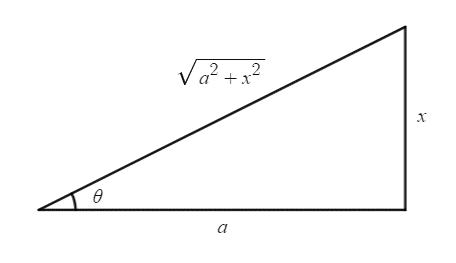
\includegraphics[scale=0.7]{IntegralCalcPictures/TrigSubTan.png}
    \item For $\sqrt{a^2-x^2}$ use $x=a\sin\theta$ where $\theta\in\brsquare{-\frac{\pi}{2},\frac{\pi}{2}}$\\
    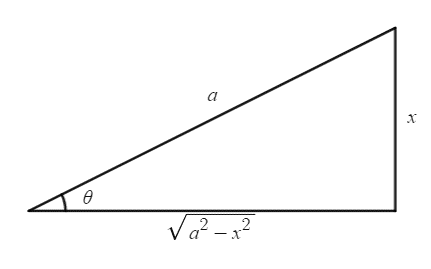
\includegraphics[scale=0.7]{IntegralCalcPictures/TrigSubSin.png}
    \item For $\sqrt{x^2-a^2}$ use $x=a\sec\theta$ where $\theta\in\left[0,\frac{\pi}{2}\right)$\\
    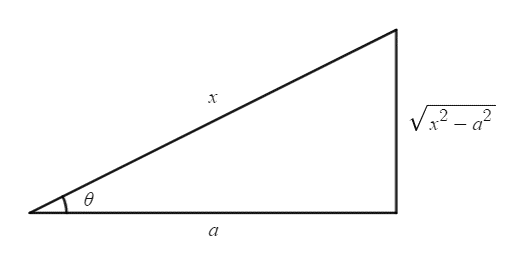
\includegraphics[scale=0.7]{IntegralCalcPictures/TrigSubSec.png}
\end{itemize}
\begin{align*}
    \text{Ex: }&\int \frac{x}{\sqrt{1-x^2}}dx\\
    &x=\sin \theta\Ra dx=\cos\theta d\theta\\
    &\sqrt{1-x^2}=\cos x\\
    &I=\int\frac{\sin\theta\cos\theta}{\cos\theta}d\theta=\int\sin\theta d\theta=-\cos\theta+C\\
    &=-\sqrt{1-x^2}+C
\end{align*}
\begin{align*}
    \text{Ex2: }&\int\frac{dx}{\sqrt{x^2+1}}\\
    &x=\tan\theta\Ra dx=\sec^2\theta d\theta\\
    &\sqrt{x^2+1}=\sec\theta\\
    &I=\int\frac{\sec^2\theta}{\sec\theta}d\theta=\ln|\sec\theta+\tan\theta|+C\\
    &=\ln|x+\sqrt{x^2+1}|+C
\end{align*}
\begin{align*}
    \text{Ex3: }&\int\frac{dx}{x^2\sqrt{x^2-16}}\\
    &x=4\sec\theta\Ra dx=4\sec\theta\tan\theta\\
    &\sqrt{x^2-16}=4\tan\theta\\
    &I=\int\frac{4\sec\theta\tan\theta}{64\sec^2\theta\tan\theta}d\theta=\frac{1}{16}\int\frac{d\theta}{\sec\theta}=\frac{1}{16}\int\cos\theta d\theta\\
    &I=\frac{\sin\theta}{16}+C\\
    &=\frac{\sqrt{x^2-16}}{16x}+C
\end{align*}
Sometimes we may be required to complete the square in order to get the expression under the square root into a form where we can perform a trig substitution
\begin{align*}
    \text{Ex: }&\int\frac{dx}{x^2+4x+7}\\
    &I=\frac{dx}{x^2+4x+4+7-4}=\int\frac{dx}{(x+2)^2+3}\\
    &\frac{x+2}{\sqrt{3}}\tan\theta\Ra dx=\sqrt{3}\sec^2\theta d\theta\\
    &\sqrt{3}\sqrt{(x+2)^2+3}=\sec^2\theta\\
    &I=\int\frac{\sqrt{3}\sec^2\theta}{3\sec^2\theta}=\int\frac{d\theta}{\sqrt{3}}=\frac{\theta}{\sqrt{3}}+C\\
    &\theta=\arctan\brround{\frac{x+2}{\sqrt{3}}}\\
    &=\frac{1}{\sqrt{3}}\arctan\brround{\frac{x+2}{\sqrt{3}}}+C
\end{align*}
\subsubsection{Partial Fractions}
Partial fractions is the method of integrating most rational functions, $\dfrac{N(x)}{D(x)}$.\\
We can split a fraction into the sum of multiple smaller fractions that are easier to solve:
$$\frac{N(x)}{D(x)}=\frac{A}{x-a}+\frac{B}{x-b}+\frac{C}{x-c}+\cdots$$
where $N(x)=A(x-b)(x-c)+B(x-a)(x-c)+C(x-a)(x-b)=\cdots$
\begin{align*}
    \text{Ex: }&\int\frac{x-3}{x^2-3x+2}dx\\
    &\frac{x-3}{x^2-3x+2}=\frac{x-3}{(x-1)(x-2)}=\frac{A}{x-1}+\frac{B}{x-2}\\
    &x-3=A(x-2)+B(x-1)\\
    &\left\{\begin{matrix} x=Ax+Bx\\
    -3=-2A-B
    \end{matrix}\right.\Ra \left\{\begin{matrix} A+B=1\\
    2A+B=3
    \end{matrix}\right.\\
    &A=2\Ra B=-1\\
    &I=\int\frac{2}{x-1}dx-\int\frac{1}{x-2}dx\\
    &=2\ln|x-1|-\ln|x-2|+C
\end{align*}
In this case, $A$ and $B$ were solved for in a system of equations. For some easy cases, we can use a "cheat" method called the cover-up method to solve for $A$ and $B$. Using the same example as above,
\begin{align*}
    &\frac{x-3}{(x-1)(x-2)}=\frac{A}{x-1}+\frac{B}{x-2}
\end{align*}
Taking the limit as $x\to 1$ makes the $B$ term insignificant and gives us an expression for $A$
\begin{align*}
    &\lim_{x\to 1}\frac{x-3}{(x-1)(x-2)}=\lim_{x\to 1}\frac{A}{x-1}\\
    &\lim_{x\to1}\frac{x-3}{x-2}=A=\frac{1-3}{1-2}=2
\end{align*}
Similarly, taking the limit as $x\to 2$ makes the $A$ term insignificant and gives us an expression for $B$
\begin{align*}
    &\lim_{x\to 2}\frac{x-3}{(x-1)(x-2)}=\lim_{x\to 2}\frac{B}{x-2}\\
    &\lim_{x\to2}\frac{x-3}{x-1}=B=\frac{2-3}{2-1}=-1
\end{align*}

Long Division Simplification:\\
If the degree of $N(x)$ is greater than or equal to the degree of $D(x)$ then we can use polynomial division to simplify:\\
\begin{align*}
    \text{Ex: }\int\frac{x^3}{x^2+x-2}dx
\end{align*}
\polylongdiv[style=A]{x^3}{x^2+x-2}
\begin{align*}
    &\frac{x^3}{x^2+x-2}=x-1+\frac{3x-2}{x^2+x-2}=x-1+\frac{3x-2}{(x-1)(x+2)}\\
    &\frac{3x-2}{(x-1)(x+2)}=\frac{A}{x-1}+\frac{B}{x+2}\\
    &\Ra A=\frac{1}{3},\,B=\frac{8}{3}\\
    &I=\int\brround{x-1+\frac{1/3}{x-1}+\frac{8/3}{x+2}}dx\\
    &=\frac{x^2}{2}-x+\frac{1}{3}\ln|x-1|+\frac{8}{3}\ln|x+2|+C
\end{align*}

Repeating Roots:\\
If the same factor is repeated in the denominator, we need to write the partial fractions slightly different.
$$\frac{N(x)}{(x-a)^n}=\frac{A_1}{x-a}+\frac{A_2}{(x-a)^2}+\frac{A_3}{(x-a)^3}+\cdots+\frac{A_n}{(x-a)^n}$$
An analogy of this using regular fractions would be
$$\frac{7}{16}=\frac{0}{2}+\frac{1}{2}+\frac{1}{2^2}+\frac{1}{2^3}+\frac{1}{2^4}$$
\begin{align*}
    \text{Ex: }&\int\frac{x^2}{(x+1)^4}dx\\
    &\frac{x^2}{(x+1)^4}=\frac{A}{x+1}+\frac{B}{(x+1)^2}+\frac{C}{(x+1)^3}+\frac{D}{(x+1)^4}\\
    &x^2=A(x+1)^3+B(x+1)^2+C(x+1)+D\\
    &\eqnsystem{&0x^3=Ax^3\\&x^2=3Ax^2+Bx^2\\&0x=3Ax+2Bx+Cx\\&0=A+B+C+D}\Ra\eqnsystem{A=0\\B=1\\C=-2\\D=1}\\
    &I=\int\brround{\frac{1}{(x+1)^2}-\frac{2}{(x+1)^3}+\frac{1}{(x+1)^4}}dx\\
    &=-\frac{1}{x+1}+\frac{1}{(x+1)^2}-\frac{1}{3(x+1)^3}+C
\end{align*}

Complex Roots:\\
This is the case in which the expression in the denominator cannot be factored completely (it will have a complex factor).\\
To solve this, we will want to split the expression so that we can make use of a u-substitution.
\begin{align*}
    \text{Ex: }&\int\frac{x+3}{x^2+2x+5}dx\\
    &u=x^2+3x+5\Ra du=(2x+2)dx\Ra \frac{du}{2}=(x+1)dx\\
    &\frac{x+3}{x^2+2x+5}=\frac{x+1+2}{x^2+2x+5}=\frac{x+1}{x^2+2x+5}+\frac{2}{x^2+2x+5}\\
    &\int\frac{x+1}{x^2+2x+5}dx=\frac{du}{2u}=\frac{1}{2}\ln|u|+C=\frac{1}{2}\ln|x^2+2x+5|+C\\
    &\int\frac{2}{x^2+2x+5}dx=\frac{2}{(x+1)^2+4}dx\\
    &\tan\theta=\frac{x+1}{2}\Ra 2\sec^2\theta d\theta=dx\\
    &2\sec\theta=\sqrt{(x+1)^2+4}\\
    &\int\frac{2}{(x+1)^2+4}=2\int\frac{2\sec^2\theta}{4\sec^2\theta}d\theta=\int d\theta=\theta+C\\
    &\theta=\arctan\brround{\frac{x+1}{2}}\\
    &\therefore I=\frac{1}{2}\ln|x^2+2x+5|+\arctan\brround{\frac{x+1}{2}}+C
\end{align*}
\begin{align*}
    \text{Ex2: }&\int\frac{2x^2-3x-7}{(x-1)(x^2+2x+5)}dx\\
    &\frac{2x^2-3x-7}{(x-1)(x^2+2x+5)}=\frac{Ax+B}{x^2+2x+5}+\frac{C}{x-1}=\frac{(Ax+B)(x-1)+C(x^2+2x+5)}{(x-1)(x^2+2x+5)}\\
    &\Ra A=3,\,B=2,\,C=-1\\
    &I=\int\frac{3x+2}{x^2+2x+5}dx-\int\frac{dx}{x-1}\\
    &u=x^2+2x+5\Ra du=(2x+2)dx\Ra \frac{du}{2}=(x+1)dx\\
    &I=\int\frac{3(x+1)}{x^2+2x+5}dx-\int\frac{1}{x^2+2x+5}dx-\int\frac{dx}{x-1}\\
    &\vdots\\
    &I=\frac{3}{2}\ln|x^2+2x+5|-\frac{1}{2}\arctan\brround{\frac{x+1}{2}}-\ln|x-1|+C
\end{align*}
\begin{align*}
    \text{Ex3: }&\int x\arctan xdx\\
    &u=\arctan x\Ra du=\frac{dx}{1+x^2}\\
    &dv=x\Ra v=\frac{x^2}{2}\\
    &I=\frac{x^2}{2}\arctan x-\frac{1}{2}\int\frac{x^2}{1+x^2}dx\\
    &\frac{x^2}{1+x^2}=\frac{x^2+1-1}{1+x^2}=1-\frac{1}{1+x^2}\\
    &\int\frac{x^2}{1+x^2}dx=\int\brround{1-\frac{1}{1+x^2}}dx=x-\arctan x +C\\
    &I=\frac{x^2}{2}\arctan x-\frac{x}{2}+\frac{1}{2}\arctan x+C
\end{align*}
\subsubsection{Separable Differential Equations}
So far, we have seen various explicit ways of finding $y$ if given $y'$. Separable differential equations are a way of doing the same for implicit equations:
\begin{align*}
    \text{for }&y'=f(x)g(y)\\
    &\frac{dy}{dx}=f(x)g(y)
\end{align*}
By approximating, we can write
\begin{align*}
    &\frac{\Delta y}{\Delta x}\approx f(x)g(y)\\
    &\frac{1}{g(y)}\Delta y\approx f(x)\Delta x\\
    &\Ra \frac{dy}{g(y)}=f(x)dx\\
    &\int \frac{dy}{g(y)}=\int f(x)dx\\
    &G(y)=F(x)+C\\
    &y=G^{-1}(F(x)+C)
\end{align*}
Essentially, we split the $x$ and $y$ components and integrate both sides to solve for $y$.\\
Ex: Find a function that passes through $(0,-1)$ and has slope $3-4x$
\begin{align*}
    &\frac{dy}{dx}=3-4x\\
    &\int dy=\int(3-4x)dx\\
    &y=3x-2x^2+C\\
    &y(0)=-1=C\\
    &\therefore y=-2x^2+3x-1
\end{align*}
Ex2: Exponential growth/decay
\begin{align*}
    &\frac{dy}{dx}=ky\\
    &\int\frac{dy}{y}=\int kdx\\
    &\ln|y|=kx+C\\
    &|y|=e^{kx+C}=Ae^{kx}\\
    &y=Ae^{kx}
\end{align*}
\begin{align*}
    \text{Ex3: }&\frac{dy}{dx}=-\frac{x}{y}\\
    &\int ydy=\int -xdx\\
    &\frac{y^2}{2}=-\frac{x^2}{2}+C\\
    &y=\sqrt{C-x^2}
\end{align*}

\subsubsection{Improper Integrals}
These are integrals that do not have nice boundaries, such as a range to infinity or with a discontinuity like $\frac{1}{x}$.\\
In these cases, we cannot treat infinity as a finite value, however, we can take the limit as it approaches infinity.\\
So, we can define
$$\int_a^\infty f(x)dx=\lim_{t\to\infty}\int_a^t f(x)dx$$
When this limit exists, the integral is said to be convergent. When the limit does not exist, the integral is said to be divergent.\\
\begin{align*}
    \text{Ex: }&\int_0^\infty e^{-x}dx=\lim_{t\to\infty}\int_0^te^{-x}dx=\lim_{t\to\infty}\brsquare{-e^{-x}}_0^t=\lim_{t\to\infty}\brround{-e^{-t}+1}=1
\end{align*}
Ex2: The $p$ test: Find all values of $p$ such that $\int_1^\infty x^pdx$ is convergent
\begin{align*}
    &\text{Case 1: }p=-1\\
    &\lim_{t\to\infty}\int_1^t\frac{dx}{x}=\lim_{t\to\infty}{\ln|x|}\eval_1^t=\lim_{t\to\infty}\ln|t|=\infty\\
    &\text{Case 2: }p\neq -1\\
    &\lim_{t\to\infty}\int_0^tx^pdx=\lim_{t\to\infty}\brsquare{\frac{x^{p+1}}{p+1}}_1^t=\lim_{t\to\infty}\brround{\frac{t^{p+1}}{p+1}-\frac{1}{p+1}}\\
    &\text{converges iff }p+1<0\Ra p<-1
\end{align*}
\begin{align*}
    \text{Ex3: }&\int_{-\infty}^\infty\frac{dx}{1+x^2}\\
    &I=\lim_{t\to\infty}\int_{-\infty}^\infty\frac{dx}{1+x^2}=\lim_{t\to\infty}{\arctan x}\eval_{-\infty}^\infty=\pi
\end{align*}
\begin{align*}
    \text{Ex4: }&\int_{-\infty}^\infty xdx\\
    &I=\int_{-\infty}^0xdx+\int_0^\infty xdx=\lim_{s\to-\infty}\int_s^0xdx+\lim_{t\to\infty}\int_0^txdx=\lim_{s\to\infty}\brsquare{\frac{x^2}{2}}_s^0+\lim_{t\to\infty}\brsquare{\frac{x^2}{2}}_0^t\\
    &I=\lim_{t\to\infty}\frac{t^2}{2}-\lim_{s\to\infty}\frac{s^2}{2}=\infty-\infty\\
    &\therefore \text{ the integral is divergent}
\end{align*}
So far, we have seen examples using bounds of infinity. Now let's see how we treat discontinuities.
Ex5: The $p$ test version 2: Find all values of $p$ such that $\int_0^1x^p$ converges
\begin{align*}
    &\text{Case 1: }p=-1\\
    &\lim_{t\to0^+}\int_t^1\frac{dx}{x}=\lim_{t\to0^+}{\ln|x|}\eval_t^1=-\lim_{t\to0^+}\ln|t|=\infty\\
    &\text{Case 2: }p\neq -1\\
    &\lim_{t\to0^+}\int_t^1x^pdx=\lim_{t\to0^+}\brsquare{\frac{x^{p+1}}{p+1}}_t^0=\lim_{t\to0^+}\frac{1}{p+1}(1-t^{p+1})\\
    &\text{converges iff }p+1>1\Ra p>-1
\end{align*}
\begin{align*}
    \text{Ex6: }&\int_0^1\ln xdx\\
    &I=\lim_{t\to0^+}\int_t^1\ln xdx=\lim_{t\to0^+}\brsquare{x\ln x-x}=-1-\lim_{t\to0^+}x\ln x\\
    &\lim_{t\to0^+}x\ln x=\lim_{t\to0^+}\frac{\ln x}{1/x}=\lim_{t\to0^+}\frac{1/x}{-1/x^2}=\lim_{t\to0^+}-x=0\\
    &I=-1
\end{align*}
By combining both $p$ test examples, we can determine that there is no such $p$ value that would allow the integral to be convergent over the entire domain.\\

Comparison Tests:\\
For integrals that are too complicated to solve, we can determine if they converge or diverge by comparing them with similar integrals we know how to solve.\\
If $|f(x)|\leq g(x)$ for all $x\geq a$ and if $\int_a^\infty g(x)dx<\infty$, then $\int_a^\infty f(x)dx<\infty$. Similarly, if $g(x)\leq f(x)$ and $\int_a^\infty g(x)dx$ diverges, so does $\int_a^\infty f(x)dx$.
\begin{align*}
    \text{Ex7: }&\text{Does }\int_1^\infty\frac{\sin^2x}{x^2}dx\text{ converge or diverge?}\\
    &0\leq\sin^2x\leq 1\Ra 0\leq \frac{\sin^2x}{x^2}\leq\frac{1}{x^2}\\
    &\int_1^\infty\frac{dx}{x^2}<\infty\\
    &\text{by comparison test, }\int_1^\infty\frac{\sin^2x}{x^2}dx\leq\int_1^\infty\frac{dx}{x^2}<\infty\\
    &\therefore \int_1^\infty\frac{\sin^2x}{x^2}dx\text{ converges}
\end{align*}











\subsection{Applications of Integrals}
\subsubsection{Area Between Curves}
We have seen how to find the area between a curve and the axis but what about the area between curves? To do this, we define a new function to be the difference between the two curves. $h(x)=f(x)-g(x)$\\
$$A=\int_b^a(f(x)-g(x))dx,\text{ for }f(x)>g(x)$$
It is important that $f(x)>g(x)$ is order to obtain a positive area. We must also pay attention to cases where the functions interlace. When this happens, we will need to split it into multiple integrals to obtain positive values.\\
Ex: Area bounded by $f(x)=x+2$ and $g(x)=x^2-4$\\
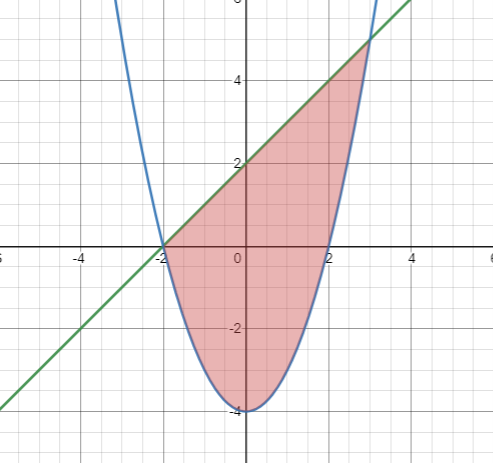
\includegraphics[scale=0.5]{IntegralCalcPictures/AreaBetweenCurvesEx1.png}
\begin{align*}
    &\text{Intercepts:}\\
    &x+2=x^2-4\\
    &x^2-x-6=0\\
    &(x-3)(x+2)=0\\
    &x=3,\,x=-2\\
    &\text{check }f(x)>g(x)\text{ for }x\in(-2,3)\\
    &A=\int_{-2}^3((x+2)-(x^2-4))dx=\int_{-2}^3(-x^2+x+6)dx=\brsquare{-\frac{x^3}{3}+\frac{x^2}{2}+6x}_{-2}^3\\
    &=\frac{125}{6}
\end{align*}
Ex2: Area bounded by $y=x^3-x$ and $y=3x$\\
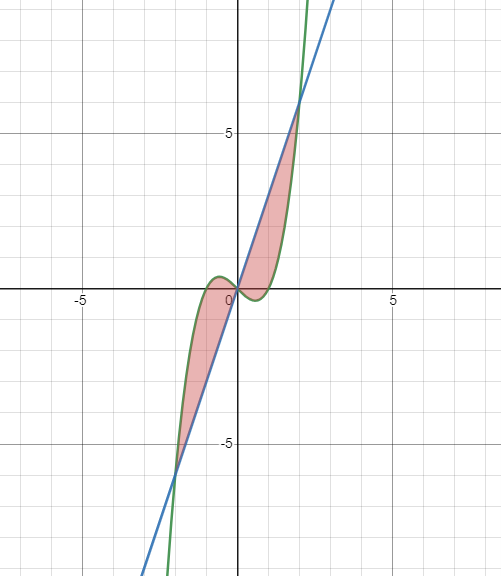
\includegraphics[scale=0.5]{IntegralCalcPictures/AreaBetweenCurvesEx2.png}
\begin{align*}
    &\text{Intercepts:}\\
    &x^3-x=3x\\
    &x^3-4x=0\\
    &x(x^2-4)=0\\
    &x=0,\,x=\pm2\\
    &x^3-x>3x\text{ for }x\in(-2,0)\\
    &3x>x^3-x\text{ for }x\in(0,2)\\
    &A=\int_{-2}^0((x^3-x)-3x)dx+\int_0^2(3x-(x^3-x))dx\\
    &A=\brsquare{\frac{x^4}{4}-2x^2}_{-2}^0+\brsquare{-\frac{x^4}{4}+2x^2}_0^2\\
    &=8
\end{align*}
Alternatively, you could have recognized this as an odd function and found the area of one sector and multiplied it by 2.\\
Sometimes it may prove easier to integrate with respect to $y$ instead of $x$.\\
Ex3: Area bounded by $y^2=4x$ and $4x-3y=4$\\
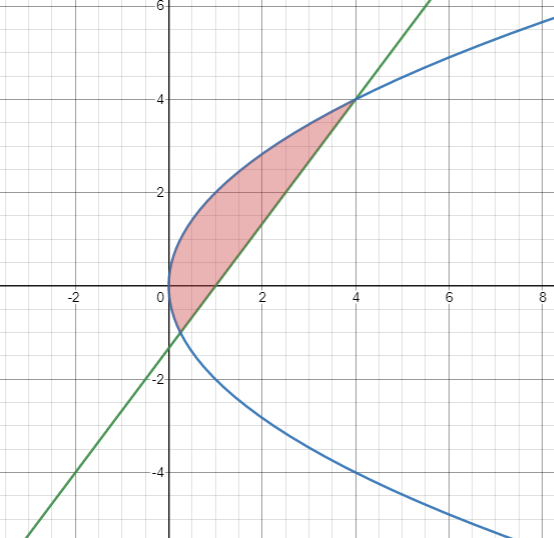
\includegraphics[scale=0.5]{IntegralCalcPictures/AreaBetweenCurvesEx3.png}
\begin{align*}
    &x=\frac{y^2}{4},\,x=\frac{3}{4}y+1\\
    &y^2=4+3y\Ra y^2-3y-4=0\\
    &(y-4)(y+1)=0\Ra y=4,\,y=-1\\
    &\frac{3}{4}y+1>\frac{y^2}{4}\text{ for }y\in(-1,4)\\
    &A=\int_{-1}^4\brround{\brround{\frac{3}{4}y+1}-\frac{y^2}{4}}dy=\brsquare{\frac{3y^2}{8}+y-\frac{y^3}{12}}_{-1}^4\\
    &=\frac{125}{24}
\end{align*}
\subsubsection{Volumes of Revolution}
Consider a function $y=f(x)$. By rotating the function about the x-axis, we can create a 3D solid of revolution.\\
Disk Method:\\
If we split our function into many different rectangles of width $\Delta x$, when we revolve our function about the x-axis, we get many disks of radius $f(x_i^*)$ and width $\Delta x$. So the volume of each disk will be $V_i=\pi (f(x_i^*))^2\Delta x$. Summing these together, we get
$$V=\lim_{n\to \infty}\sum_{i=1}^n\pi(f(x_i^*))^2\Delta x=\pi\int_a^b(f(x))^2dx$$
Ex: Find the volume of the cone formed by rotating $y=\frac{x}{2}$ about the x-axis on the interval $[0,6]$
\begin{align*}
    V=\pi\int_0^6\brround{\frac{x}{2}}^2dx=\frac{\pi}{4}\int_0^6x^2dx={\frac{\pi x^3}{12}}\eval_0^6=18\pi
\end{align*}
Ex2: Find the volume of the sphere formed by rotating $y=\sqrt{r^2-x^2}$ about the x-axis
\begin{align*}
    V&=\pi\int_{-r}^r(r^2-x^2)dx=\pi\brsquare{r^2x-\frac{x^3}{3}}_{-r}^r\\
    &=\frac{4}{3}\pi r^3
\end{align*}
If we are dealing with multiple sections we can compute the volumes independently and subtract the inner volume from the outer volume
$$V=V_{outer}-V_{inner}$$
Ex3: Find the volume of the bowl formed by rotating the area bounded by $\sqrt{3-3x}$ and $\sqrt{1-x^2}$ between $x=0$ and $x=1$
\begin{align*}
    &\sqrt{3-3x}>\sqrt{1-x^2}\text{ for }x\in[0,1)\\
    &\text{Outer: }\sqrt{3-3x}\\
    &\text{Inner: }\sqrt{1-x^2}\\
    &V=\pi\int_0^1\brround{(3-3x)-(1-x^2)}dx=\pi\brsquare{2x-\frac{3}{2}x^2+\frac{x^3}{3}}_0^1\\
    &=\frac{5\pi}{6}
\end{align*}
Using the disk method, if you rotate about the x-axis, you must integrate with respect to $x$. If you rotate about the y-axis, you must integrate with respect to $y$.\\
If you are rotating about any axis other than the x or y-axis, (such as the line $y=3$, you must translate all functions so that you are rotating about the x or y-axis.\\
Ex4: Find the volume of the solid generated by rotating the region bounded by $y=0$, $x=4$, and $y=\sqrt{x}$ about the line $x=6$
\begin{align*}
    &\text{Integrate with respect to $y$: }y=\sqrt{x}\Ra x=y^2\\
    &\text{Outer: }x=y^2\\
    &\text{Inner: }x=4\\
    &\text{Bounds: }x=0\Ra y=0,\,x=4\Ra y=2\\
    &V=\pi\int_{y=0}^{y=2}\brround{(y^2)^2-(4)^2}dy\\
    &\text{Shift: }x\to x-6\\
    &V=\pi\int_0^2\brround{(y^2-6)^2-(-2)^2}dy\\
    &V=\pi\brsquare{\frac{y^5}{5}-4y^3+32y}_0^2\\
    &=\frac{192}{5}\pi
\end{align*}
Shell Method:\\
An alternative way to find area is using shells. This involves finding the are of each shell of the solid like the layers of an onion.\\
The general expression is
$$V=\int_a^b2\pi rhdr$$\\
Depending on your variable of integration, $r$ and $h$ will take the values of $x$ or $y$\\
Ex5: Using the same example as before: Find the volume of the solid generated by rotating the region bounded by $y=0$, $x=4$, and $y=\sqrt{x}$ about the line $x=6$
\begin{align*}
    &h=\sqrt{x}\\
    &r=6-x\\
    &V=2\pi\int_0^4(6-x)\sqrt{x}dx\\
    &V=2\pi\brsquare{4x^{3/2}+\frac{2}{5}x^{5/2}}_0^4\\
    &=\frac{192}{5}\pi
\end{align*}

\subsubsection{Arc Length}
Calculus is founded on the basis that any line is straight if we zoom in enough. This interpretation is very helpful when computing the length of a curve\\
\includegraphics[scale=0.7]{IntegralCalcPictures/ArcLengthTriangle.png}
\begin{align*}
    &(\Delta s)^2\approx (\Delta x)^2+(\Delta y)^2\\
    &\to(ds)^2=(dx)^2+(dy)^2\\
    &ds=\sqrt{(dx)^2+(dy)^2}\\
    &ds=\sqrt{(dx)^2+(dy)^2}\brround{\frac{dx}{dx}}\\
    &ds=\sqrt{1+\brround{\frac{dy}{dx}}^2}dx\\
    &s=\int_b^a\sqrt{1+(f'(x))^2}dx
\end{align*}
where $s$ is the arc length.\\
Ex: Find the arc length of a semicircle or radius 1
\begin{align*}
    &y=\sqrt{1-x^2}\\
    &y'=\frac{-x}{\sqrt{1-x^2}}\\
    &ds=\sqrt{1+\frac{x^2}{1-x^2}}=\sqrt{\frac{1}{1-x^2}}\\
    &s=\int_{-1}^1\frac{dx}{\sqrt{1-x^2}}={\arcsin x}\eval_{-1}^1\\
    &=\pi
    \end{align*}
Ex2: Find the length of the parabola $y=x^2$ from 0 to $a$
\begin{align*}
    &y=x^2\Ra y'=2x\\
    &ds=\sqrt{1+4x^2}dx\\
    &s=\int_0^a\sqrt{1+4x^2}dx\\
    &\vdots\\
    &=\brsquare{\frac{1}{4}\ln|2x+\sqrt{1+4x^2}|+\frac{1}{2}x\sqrt{1+4x^2}}_0^a
\end{align*}
\subsubsection{Surface Area}
We can compute some surface areas using rotations and by calculating the surface of rotation.\\
Similar to volumes of revolution, we can compute the surface area using rings: ${dS=\text{circumference}\cdot ds}$\\
$\Ra dS=2\pi y ds$\\
Ex: Find the surface area of a sphere of radius $r$
\begin{align*}
    &y=\sqrt{r^2-x^2}\\
    &y'=\frac{-x}{r^2-x^2}\\
    &ds=\sqrt{1+\frac{x^2}{r^2-x^2}}dx=\sqrt{\frac{r^2}{r^2-x^2}}dx\\
    &S=\int_{-r}^r2\pi\sqrt{r^2-x^2}\sqrt{\frac{r^2}{r^2-x^2}}dx=2\pi\int_{-r}^r rdx\\
    &S={2\pi rx}\eval_{-r}^r\\
    &=4\pi r^2
\end{align*}
Ex2: Find the surface area of a torus (doughnut). Let $R$ be the distance from the hole to the center of the solid and let $r$ be the internal radius.
\begin{align*}
    &(x-R)^2+y^2=r^2\\
    &y=\sqrt{r^2-(x-R)^2}\\
    &y'=\frac{-(x-R)}{r^2-(x-R)^2}\\
    &ds=\sqrt{1+\frac{(x-R)^2}{r^2-(x-R)^2}}dx=\frac{r}{\sqrt{r^2-(x-R)^2}}dx\\
    &dS=\frac{2\pi rx}{\sqrt{r^2-(x-R)^2}}dx\Ra S=2\pi r\int_{R-r}^{R+r}\frac{x}{\sqrt{r^2-(x-R)^2}}\\
    &u=x-R\Ra x=u+R\Ra du=dx\\
    &S=2\pi r\int_{-r}^r\frac{u+R}{\sqrt{r^2-u^2}}du=2\pi r\brround{\int_{-r}^r\frac{u}{\sqrt{r^2-u^2}}+R\int_{-r}^r\frac{du}{\sqrt{r^2-u^2}}}\\
    &\text{note that }\int_{-r}^r\frac{u}{\sqrt{r^2-u^2}}\text{is odd so it will be 0}\\
    &\Ra S=4\pi rR\int_{0}^r\frac{du}{\sqrt{r^2-u^2}}=4\pi rR{\arcsin\brround{\frac{u}{r}}}\eval_0^r\\
    &=4\pi^2rR
\end{align*}

\subsubsection{Work}
Work is defined to be $W=F\cdot x$\\
Ex: How much work is required to bring a book of 1kg to a height of 2m?
\begin{align*}
    &F=mg=9.81\\
    &W=F\cdot x=(9.81)(2)=19.62J
\end{align*}
If the force is not constant then we can break the action into small parts and sum them up: $dW=dF\cdot dx$. This gives a definition of work to be
$$W=\int_a^bF(x)dx$$
Ex2: A string has a length of 30cm (unstretched). A force of 20N is required to keep it stretched at a length of 40cm. How much work is required to stretch it from 30cm to 35cm? Note $F=kx$
\begin{align*}
    &\text{find $k$: }F(x)=kx,\,x=0.4-0.3=0.1m\\
    &F(0.1)=20=0.1k\Ra k=200N/m\\
    &W=\int_0^{0.05}F(x)dx=\int_0^{0.05}200xdx={100x^2}\eval_0^{0.05}\\
    &=0.25J
\end{align*}

\subsubsection{Average Value}
The average of a set of $n$ discrete values is defined as
$$\overline{x}=\frac{\sum\limits_{i=1}^nx_i}{n}$$
For a continuous function, the average is defined as
$$\overline{f(x)}=\frac{1}{b-a}\int_a^bf(x)dx$$
This formula is derived from the Mean Value Theorem:
\begin{align*}
    &\text{For }f(x)=F'(x),\\
    &f(c)=\frac{F(b)-F(a)}{b-a}\\
    &\int_a^bf(x)dx=F(b)-F(a)\\
    &\therefore\,f(c)=\frac{1}{b-a}\int_a^bf(x)dx=\overline{f(x)}
\end{align*}
Ex: Find the average height of the point on a semicircle.
\begin{align*}
    &\overline{y}=\frac{1}{r-(-r)}\int_{-r}^r\sqrt{r^2-x^2}dx\\
    &\text{let }x=r\sin\theta\Ra dx=r\cos\theta d\theta\\
    &\sqrt{r^2-x^2}=r\cos\theta\\
    &\theta=\arcsin\brround{\frac{x}{r}}\\
    &\frac{1}{2r}\int_{x=-r}^{x=r}r^2\cos\theta d\theta=\frac{r}{2}\int_{x=-r}^{x=r}\frac{1+\cos2\theta}{2}d\theta=\frac{r}{4}\brsquare{\theta+\frac{1}{2}\sin2\theta}_{x=-r}^{x=r}=\frac{r}{4}\brsquare{\theta+\frac{1}{2}\sin\theta\cos\theta}_{x=-r}^{x=r}\\
    &\overline{y}=\frac{r}{4}\brsquare{\arcsin\brround{\frac{x}{r}}+\frac{1}{2}\brround{\frac{\sqrt{r^2-x^2}}{r}}\brround{\frac{x}{r}}}_{-r}^r\\
    &=\frac{\pi r}{4}
\end{align*}
A common application is time averages. This is the average value of a periodic function over one period, denoted by $\brangle{f(x)}$. By inspection, the time average of $\sin x$ or $\cos x$ is 0, however, we can take the root mean squared average (RMS) instead to get a non-zero value.\\
Ex2: Compute the RMS average of $\cos x$: $\sqrt{\brangle{\cos^2x}}$
\begin{align*}
    &\brangle{\cos^2x}=\frac{1}{\pi}\int_0^\pi\cos^2xdx=\frac{1}{2\pi}\int_0^\pi(1+\cos2x)=\frac{1}{2\pi}\brsquare{x+\frac{1}{2}\sin x\cos x}_0^\pi\\
    &=\frac{1}{2}\\
    &\Ra\sqrt{\brangle{\cos^2x}}=\frac{1}{\sqrt{2}}
\end{align*}
Ex3: Average speed: Let $v(t)$ be the speed of a particle over $t_0\leq t\leq t_1$. What is the average speed of $t$?
\begin{align*}
    &\overline{v}=\frac{1}{t_1-t_0}\int_{t_0}^{t_1}v(t)dt={\frac{1}{t_1-t_0}x(t)}\eval_{t_0}^{t_1}=\frac{x(t_1)-x(t_0)}{t_1-t_0}=\frac{\Delta x}{\Delta t}
\end{align*}
Ex4: Find all positive values of $b$ such that the average of $f(x)=10-x^2$ on the interval $0\leq x\leq b$ is equal to 1.
\begin{align*}
    &1=\frac{1}{b-0}\int_0^b(10-x^2)dx=\frac{1}{b}\brsquare{10x-\frac{x^3}{3}}_0^b=10-\frac{b^3}{3}\\
    &\frac{b^2}{3}=9\Ra b^2=27\Ra b=\pm\sqrt{27}\\
    &b=\sqrt{27}
\end{align*}
\subsubsection{Weighted Averages}
Sometimes when taking an average, we may want to value certain points more and take a weighted average instead. A common example is when considering an object's center of mass.\\
Considering the simple case of discreet masses on a lever. The center of mass will be the location in which to place a fulcrum so that the torque on both sides of the lever is balanced. $\tau_{cw}=\tau_{ccw}$ where $\tau=F\times d=mgd$ where $d$ is the distance from the fulcrum. For discrete masses, we can express this as
$$\overline{x}=\frac{\ds\sum_{i=1}^Nm_ix_i}{\ds\sum_{i=1}^Nm_i}$$
Ex: If we have a 2kg weight at $x=1$ and a 1kg weight at $x=5$, what is the center of mass?
\begin{align*}
    \overline{x}\frac{(2)(1)+(1)(5)}{2+1}=\frac{7}{3}
\end{align*}
For continuous mass distributions, we can express the mass as the sum of a function of density:
$$\overline{x}=\frac{\ds\int_a^bx\mu(x)dx}{\ds\int_a^b\mu(x)dx}$$
Ex: A metal rod is 50cm long. Its density is given by $\mu(x)=\dfrac{1}{100-x}$ for $0\leq x\leq 50$
\begin{align*}
    \overline{x}&=\frac{\ds\int_0^{50}\frac{x}{100-x}dx}{\ds\int_0^{50}\frac{dx}{100-x}}=\frac{\ds\int_0^{50}\frac{x}{100-x}dx}{\ds\int_0^{50}\brround{\frac{x-100}{100-x}+\frac{100}{100-x}}dx}\\
    &=\frac{\ds{-\ln|100-x|}\eval_0^{50}}{\ds{\brround{-x-100\ln|100-x|}}\eval_0^{50}}\\
    &=\frac{-50+100\ln 2}{\ln 2}=100-\frac{50}{\ln 2}\approx 28.06cm
\end{align*}
The more general expression of a weighted average is
$$\overline{f(x)}=\frac{\displaystyle{\int_a^bf(x)w(x)dx}}{\displaystyle{\int_a^bw(x)dx}}$$
where $w(x)$ is the weighting applied.\\
Notice in the example of center of mass, $f(x)=x$ and $w(x)=\mu(x)$\\
Ex2: Let $R$ be the region bounded above the x-axis by $y=x$ and $y=x^3$. What is the average x-coordinate of $R$?
\begin{align*}
    &\text{Want average of $f(x)=x$ over $R$}\\
    &f(x)=x,\,w(x)=x-x^3\\
    &\mathrm{Avg}=\frac{\ds\int_0^1x(x-x^3)dx}{\ds\int_0^1(x-x^3)dx}=\frac{2/15}{1/4}=\frac{8}{15}
\end{align*}
\\
Probability:\\
We use the method of weighted averages to calculate probabilities as well.\\
Ex: Pick a point at random in $0<y<1-x^2$ (the area under the parabola). What is the probability that $x>\frac{1}{2}$?
\begin{align*}
    &P\brround{x>\frac{1}{2}}=\frac{\displaystyle{\int_{\frac{1}{2}}^1(1-x^2)dx}}{\displaystyle{\int_{-1}^1(1-x^2)dx}}\\
    &P=\frac{\ds\brsquare{x-\frac{x^3}{3}}_{\frac{1}{2}}^1}{\ds\brsquare{x-\frac{x^3}{3}}_{-1}^1}=\frac{15}{96}
\end{align*}







































% Series and Transforms

\section{Series and Transforms}
\subsection{Sequences and Series}
\subsubsection{Convergence of Sequences and Series}
Recall, a sequence is a list of infinitely many numbers with a specified order
$$\brcurly{a_n=f(n)}_{n=1}^\infty=\brcurly{a_1,\,a_2\,a_3,\ldots,\,a_n}$$
A sequence converges if $a_n$ approaches $A$ as $n\to\infty$.
\begin{align*}
    \lim_{n\to\infty}a_n=A
\end{align*}
\begin{align*}
    \text{Ex: }\brcurly{a_n=\frac{1}{n}}_{n=1}^\infty=\lim_{n\to\infty}\frac{1}{n}=0
\end{align*}
\begin{align*}
    \text{Ex2: }\brcurly{a_n=(-1)^n}_{n=0}^\infty=\brcurly{1,-1,1,-1,\ldots}\therefore\text{ divergent}
\end{align*}
\begin{align*}
    \text{Ex3: }\brcurly{\frac{2x^2+3}{n^2+n}}_{n=1}^\infty=\lim_{n\to\infty}\frac{2n^2+3}{n^2+n}=2
\end{align*}

A series is when all the terms of a sequence are summed.\\
Geometric Series:
$$\sum_{n=1}^\infty ar^n=\frac{a}{1-r}\text{ if $|r|<1$}$$
where $a$ is the first term in the series and $r$ is the common ratio.
Proof:
\begin{align*}
    &S_N=\sum_{n=1}^\infty ar^n=a(1+r+r^2+\cdots+r^N)\\
    &rS_N=a(r+r^2+r^3+\cdots+r^N+r{N+1}\\
    &rS_N-S_N=a(r+r^2+r^3+\cdots+r^N+r{N+1}-S_N=a(r^{N+1}-1)\\
    &(1-r)S_N=a(1-r^{N+1})\\
    &S_N=\frac{a(1-r^{N+1})}{1-r}\\
    &S_\infty=\frac{a}{1-r}
\end{align*}
Ex: find the infinite sum of ${S=9-\frac{27}{5}+\frac{81}{25}-\frac{243}{125}+\cdots}$
\begin{align*}
    &S=9\brround{1-\frac{3}{5}+\brround{\frac{3}{5}}^2-\brround{\frac{3}{5}}^3+\cdots}\\
    &a=9,\,r=-\frac{3}{5}\\
    &|r|<1\,\therefore\,\text{convergent}\\
    &S_\infty=\frac{a}{1-r}=\frac{9}{1-3/5}=\frac{45}{8}
\end{align*}
\begin{align*}
    \text{Ex2: }&S=\sum_{n=1}^\infty\frac{4^n+5^n}{9^n}\\
    &S=\sum_{n=1}^\infty\brround{\frac{4}{9}}^n+\sum_{n=1}^\infty\brround{\frac{5}{9}}^n\\
    &S=\frac{4/9}{1-4/9}+\frac{5/9}{1-5/9}=\frac{41}{20}
\end{align*}
\begin{align*}
    \text{Ex3: }&\sum_{n=0}^\infty\frac{3^n}{8^{2n+1}}\\
    &S=\frac{1}{8}\sum_{n=0}^\infty\frac{3^n}{8^{2n}}=\frac{1}{8}\sum_{n=0}^\infty\brround{\frac{3}{8^2}}^n=\frac{1/8}{1-3/64}=\frac{8}{61}
\end{align*}
\begin{align*}
    \text{Ex4: }&\text{write the decimal $0.1\overline{23}$ as a fraction}\\
    &0.1\overline{23}=\frac{1}{10}+\frac{23}{10^3}+\frac{23}{10^5}+\cdots=\frac{1}{10}+\frac{12}{10^3}\sum_{n=0}^\infty\brround{\frac{1}{100^n}}\\
    &S=\frac{1}{10}+\frac{23/1000}{1-1/100}=\frac{122}{990}
\end{align*}

Telescoping Series:
Telescoping series are typically in the form of
$$S=\sum_{n=1}^\infty(a_n-a_{n+1})=(a_1-a_2)+(a_2-a_3)+\cdots+(a_{N-1}-a_N)=a_1-a_N$$
\begin{align*}
    &S_\infty=\lim_{N\to\infty}(a_1-a_N)\\
    &\text{if }\lim_{N\to\infty}a_N=A\\
    &\text{then }S_\infty=a_1-A
\end{align*}
\begin{align*}
    \text{Ex: }&\sum_{n=1}^\infty\frac{1}{n(n+1)}\\
    &=\sum_{n=1}^\infty\brround{\frac{1}{n}-\frac{1}{n+1}}\\
    &\text{set }a_n=\frac{1}{n}\Ra \lim_{n\to\infty}a_n=0\\
    &S=a_1-A=1-0=1
\end{align*}
\begin{align*}
    \text{Ex2: }&\sum_{n=3}^\infty\brround{\cos\brround{\frac{\pi}{n}}-\cos\brround{\frac{\pi}{n+1}}}\\
    &=\cos\frac{\pi}{3}-\cos\frac{\pi}{4}+\cos\frac{\pi}{4}-\cos\frac{\pi}{5}+\cdots\\
    &S=\cos\brround{\pi}{3}-\lim_{N\to\infty}\cos\brround{\frac{\pi}{N+1}}=\frac{1}{2}-1=-\frac{1}{2}
\end{align*}
\begin{align*}
    \text{Ex3: }&\sum_{n=1}^\infty\ln\brround{1+\frac{1}{n}}\\
    &\sum_{n=1}^\infty\ln\brround{\frac{n+1}{n}}=\sum_{n=1}^\infty(\ln(n+1)-\ln(n))\\
    &S=\ln2-\ln1+\ln3-\ln2+\cdots+\ln(N+1)-\ln(N)\\
    &S=-\ln1+\ln(N+1)\to\infty\\
    &\therefore \text{ series diverges}
\end{align*}

\subsubsection{Convergence Tests}
\textbf{Divergence Theorem:}\\
If $\{a_n\}_{n=1}^\infty$ does not converge to 0, then $\displaystyle{\sum_{n=1}^\infty a_n}$ diverges\\
\begin{align*}
    \text{Ex: }&\sum_{n=1}^\infty\frac{2n+1}{4n+4}\text{ diverges because }\lim_{n\to\infty}\frac{2n+1}{4n+4}\neq 0
\end{align*}
\textbf{Integral Test:}\\
The integral test allows us to compare the convergence of sums to those of integrals of the same function such that for $f(n)=a_n$, $f(x)>0$ and $f'(x)<0$, we get that
\begin{align*}
    &\text{if }\int_{N_0}^\infty f(x)dx\text{ converges, then }\sum_{n=N_0}^\infty a_n\text{ converges}\\
    &\text{if }\int_{N_0}^\infty f(x)dx\text{ diverges, then }\sum_{n=N_0}^\infty a_n\text{ diverges}
\end{align*}
The sums and integrals compare in the following way:\\
$$\left|\sum_{n=a}^\infty f(n)-\int_a^\infty f(x)dx\right|<f(a)$$
More simply put,
$$\sum_{n=2}^\infty f(n)=\sum_{n=1}^\infty f(n)-a_1\leq\int_1^\infty f(x)dx\leq \sum_{n=1}^\infty f(n)$$
Ex: For what values of $p\geq 0$ does $\displaystyle{\sum_{n=2}^\infty\frac{1}{n(\ln(n))^p}}$ converge?
\begin{align*}
    &f(x)=\frac{1}{x(\ln x)^p},\,N_0=2\\
    &I=\int_2^\infty\frac{dx}{x(\ln x)^p}\\
    &u=\ln x\Ra du=\frac{dx}{x}\\
    &I=\int_{\ln2}^{\ln\infty}\frac{du}{u^p}\\
    &\therefore\text{ by $p$ test, converges only if }p>1
\end{align*}
We can also use the integral test to estimate remainders.\\
$R_N=S_\infty-S_N$. So $R_N$ is essentially the tail of the series: $R_N=a_{N+1}+a_{N+2}+\cdots$
$$\int_{N+1}^\infty<R_N<\infty_N^\infty f(x)dx$$
\begin{align*}
    \text{Ex: }&\text{Estimate $R_{100}$ for }\sum_{n=1}^\infty\frac{1}{n^2}\\
    &\text{let }f(x)=\frac{1}{x^2}\\
    &\int_{101}^\infty\frac{dx}{x^2}<R_{100}<\int_{100}^\infty\frac{dx}{x^2}\\
    &\frac{1}{101}<R_{100}<\frac{1}{100}
\end{align*}
This means that the tail of the series in this example only impacts the 2nd decimal place\\
\textbf{Comparison Test:}\\
If $|a_n|\leq c_n$ and $\sum c_n$ converges, then $\sum a_n$ converges
\begin{align*}
    \text{Ex: }\sum_{n=1}^\infty\frac{1}{n^2}\text{ converges and }\frac{1}{n^2+1}<\frac{1}{n^2}\,\therefore\,\sum_{n=1}^\infty\frac{1}{n^2+1}\text{ converges}
\end{align*}
\textbf{Limit Comparison Test:}\\
If $\displaystyle{\lim_{n\to\infty}\frac{a_n}{b_n}=L}$ for $L\neq 0$ then the convergence of $a_n$ will math the convergence of $b_n$. i.e. if $b_n$ diverges then so must $a_n$.\\
We choose $b_n$ such that we know its convergence and it provides useful information
\begin{align*}
    \text{Ex: }&\sum_{n=1}^\infty\frac{n^2+\sin(n)}{n^4}\\
    &\text{set }b_n=\frac{1}{n^2}\\
    &\lim_{n\to\infty}\frac{a_n}{b_n}=\lim_{n\to\infty}\frac{\ds\brround{\frac{n^2+\sin(n)}{n^4}}}{\ds\brround{\frac{1}{n^2}}}=1\\
    &\text{limit exists and }L\neq 0\text{ so limit comparison test is valid}\\
    &b_n\text{ converges }\therefore\,a_n\text{ converges}
\end{align*}
\textbf{Alternating Series Test:}\\
For $a_n=(-1)^nb_n$ and $|a_n|\geq|a_{n+1}|$ then if $\displaystyle{\lim_{n\to\infty}|a_n|}=0$, $\sum a_n$ converges
\begin{align*}
    \text{Ex: }&\sum_{n=1}^\infty(-1)^{n-1}\frac{\sqrt{n}}{n+4}\\
    &b_n=\frac{\sqrt{n}}{n+4}\Ra b_n'=\frac{\ds\frac{n+4}{2\sqrt{n}}-\sqrt{n}}{\ds(n+4)^2}<0\text{ if }n>4\\
    &\lim_{n\to\infty}b_n=0\\
    &\therefore\text{ by the alternating series test, the series converges}
\end{align*}
We estimate the remainder of an alternating series using
$$R_N=|S-S_N|\leq b_{n+1}$$
Ex: How many terms are needed to get an error of $2.5\cdot 10^{-8}$ for $e^{-1}$
\begin{align*}
    &\text{recall }e^x=\sum_{n=0}^\infty\frac{x^n}{n!}\\
    &e^{-1}=\sum_{n=0}^\infty\frac{(-1)^n}{n!}\\
    &R_N=|S-S_N|\leq\frac{1}{(N+1)!}\Ra \brvertical{\frac{1}{e}\leq \frac{1}{(N+1)!}}\\
    &\text{guess }N=10\Ra \frac{1}{(10+1)!}\sim2.5\cdot10^{-8}
\end{align*}
\textbf{Absolute and Conditional Convergence:}\\
If $\sum|a_n|$ converges then $\sum a_n$ is said to converge absolutely\\
If $\sum a_n$ converges but $\sum|a_n|$ diverges then $\sum a_n$ is said to be conditionally convergent\\
\begin{align*}
    \text{Ex: }&\sum_{n=1}^\infty\frac{(-1)^n}{n}\\
    &|a_n|=\frac{1}{n}\\
    &\sum_{n=1}^\infty\frac{1}{n}\text{ diverges by the integral test}\\
    &\therefore\text{ the series is conditionally convergent}
\end{align*}
\begin{align*}
    \text{Ex2: }&\sum_{n=1}^\infty\frac{(-1)^n}{n^2}\\
    &|a_n|=\frac{1}{n^2}\\
    &\sum_{n=1}^\infty\frac{1}{n^2}\text{ converges by the integral test}\\
    &\therefore\text{ the series is absolutely convergent}
\end{align*}
\textbf{Ratio Test:}\\
The ratio test is set up in the form
$$\lim_{n\to\infty}\brvertical{\frac{a_{n+1}}{a_n}}=L$$
If $L>1$, $a_n$ diverges\\
If $L<1$, $a_n$ converges\\
If $L=1$, the test fails and does not tell us anything about the convergence
\begin{align*}
    \text{Ex: }&\sum_{n=1}^\infty(-1)\frac{n!}{5^n}\\
    &\lim_{n\to\infty}\brvertical{\frac{a_{n+1}}{a_n}}=\lim_{n\to\infty}\frac{\ds\brround{\frac{(n+1)!}{5^{n+1}}}}{\ds\brround{\frac{n!}{5^n}}}=\lim_{n\to\infty}\frac{5^n}{5^{n+1}}\cdot\frac{(n+1)!}{n!}=\lim_{n\to\infty}\frac{n+1}{5}=\infty\\
    &\therefore\text{ the series diverges}
\end{align*}

\subsubsection{Power Series}
A power series is a particular series in the form of
$$\sum_{n=0}^\infty A_n(x-c)^n=A_0+A_1(x-c)+A_2(x-c)^2+\cdots$$
$\displaystyle{\sum_{n=0}^\infty A_n(x-c)^n}$ converges if $|x-c|<R$ and diverges if $|x-c|>R$ for where $R$ is the radius of convergence.\\
\begin{align*}
    \text{Ex: }&\sum_{n=0}^\infty\frac{x^n}{n!}\\
    &\lim_{n\to\infty}\brvertical{\frac{a_n}{a_{n+1}}}=|x|\lim_{n\to\infty}\brround{\frac{1}{n+1}}=0\\
    &\therefore\text{ series converges for all $x$}\\
    &\Ra R=\infty
\end{align*}
\begin{align*}
    \text{Ex2: }&\sum_{n=0}^\infty n!x^n\\
    &\lim_{n\to\infty}\brvertical{\frac{a_n}{a_{n+1}}}=|x|\lim_{n\to\infty}(n+1)=\eqnsystem{\infty\text{ if }x\neq 0\\0\text{ if }x=0}\\
    &\text{series converges only if }x=0\\
    &\therefore\,R=0
\end{align*}
\begin{align*}
    \text{Ex3: }&\sum_{n=1}^\infty(-1)^{n-1}\frac{x^n}{n}\\
    &\lim_{n\to\infty}\brvertical{\frac{a_n}{a_{n+1}}}=|x|\lim_{n\to\infty}\frac{n}{n+1}=|x|\\
    &\text{series is convergent if $|x|<1$ and divergent if $|x|>1$}\\
    &\therefore\, R=1\\
    &\text{but what if $|x|=1$?}\\
    &\text{Endpoint $x=1$: }\sum_{n=1}^\infty(-1)^{n-1}\frac{1}{n}\to\text{convergent by alternating series test}\\
    &\text{Endpoint $x=-1$: }\sum_{n=1}^\infty(-1)^{2n-1}\frac{1}{n}=-\sum_{n=1}^\infty\frac{1}{n}\to\text{divergent by integral test}\\
    &\Ra x\in(-1,1]
\end{align*}
This range of $x$ values is called the interval of convergence\\
\\
We can use power series to define functions as series. For example the geometric series is expressed as ${1+x+x^2+\cdots}$. The infinite sum works out to be $\dfrac{1}{1-x}$ using the formula $\dfrac{1}{1-r}$. From here (or by using Taylor expansion) we can express many functions as series.\\
Note that the Taylor series a special type of Power series that is defined as
$$\sum_{n=0}^\infty\frac{f^{(n)}(a)}{n!}(x-a)^n$$
\begin{align*}
    \text{Ex: }&\text{show }\ln(1+x)=\sum_{n=0}^\infty(-1)^n\frac{x^{n+1}}{n+1}\text{ for }|x|<1\\
    &\frac{1}{1-x}=\sum_{n=0}^\infty x^n\\
    &\text{sub $x$ for $-x$: }\frac{1}{1+x}=\sum_{n=0}^\infty(-1)^nx^n\\
    &\text{integrate: }\int\frac{dx}{1+x}=\sum_{n=0}^\infty(-1)^n\int x^ndx\\
    &\ln|1+x|=\sum_{n=0}^\infty(-1)^n\frac{x^{n+1}}{n+1}+C\\
    &x=0:\,\ln(1)=0=\sum_{n=0}^\infty(-1)^n\frac{x^{n+1}}{n+1}+C\Ra C=0\\
    &\therefore\,\ln|1+x|=\sum_{n=0}^\infty(-1)^n\frac{x^{n+1}}{n+1}
\end{align*}
Ex2: define the error function using power series.
\begin{align*}
    &\erf(x)=\frac{2}{\sqrt{\pi}}\int_0^xe^{-t^2}dt\\
    &e^x=\sum_{n=1}^\infty\frac{x^n}{n!}\\
    &e^{-t^2}=\sum_{n=1}^\infty\frac{(-t^2)^{n}}{n!}=\sum_{n=1}^\infty\frac{(-1)^nt^{2n}}{n!}\\
    &\int_0^x e^{-t^2}dt=\brsquare{\sum_{n=1}^\infty\frac{(-1)^nt^{2n+1}}{(2n+1)n!}}_0^x\\
    &\erf(x)=\frac{2}{\sqrt{\pi}}\sum_{n=1}^\infty\frac{(-1)^nx^{2n+1}}{(2n+1)n!}
\end{align*}
\begin{align*}
    \text{Ex3: }&\text{Which function is defined by the series }\sum_{n=0}^\infty n^2x^n\text{?}\\
    &\frac{1}{1-x}=\sum_{n=0}^\infty x^n\\
    &\frac{d}{dx}\brround{\frac{1}{1-x}}=\sum_{n=0}^\infty\frac{d}{dx}x^n\\
    &\frac{1}{(1-x)^2}=\sum_{n=0}^\infty nx^{n-1}\\
    &\frac{x}{(1-x)^2}=\sum_{n=0}^\infty nx^n\\
    &\frac{d}{dx}\frac{x}{(1-x)^2}=\sum_{n=0}^\infty\frac{d}{dx} nx^n\\
    &\frac{1-3x}{(1-x)^3}=\sum_{n=0}^\infty n^2x^{n-1}\\
    &\frac{x(1-3x)}{(1-x)^3}=\sum_{n=0}^\infty n^2x^n\\
\end{align*}
Some of the more common Power series you'll see are compiled in this list:
\begin{align*}
    &\frac{1}{1-x}=\sum_{n=0}^\infty x^n\text{ for $|x|<1$}\\
    &e^x=\sum_{n=0}^\infty\frac{x^n}{n!}\\
    &\ln(1+x)=\sum_{n=0}^\infty(-1)^n\frac{x^{n+1}}{n+1}\text{ for $|x|<1$}\\
    &\arctan x=\sum_{n=0}^\infty(-1)^n\frac{x^{2n+1}}{2n+1}\text{ for $|x|<1$}\\
    &\sin x=\sum_{n=0}^\infty(-1)^n\frac{x^{2n+1}}{(2n+1)!}\\
    &\cos x=\sum_{n=0}^\infty(-1)^n\frac{x^{2n}}{(2n)!}\\
    &(1+x)^p=\sum_{n=0}^\infty\frac{p!}{n!(p-n)!}x^n=1+px+\frac{p(p-1)}{2!}x^2+\frac{p(p-1)(p-2)}{3!}x^3+\cdots
\end{align*}
These Taylor series are useful in solving some otherwise difficult problems
\begin{align*}
    \text{Ex: }&\lim_{x\to0}\frac{\cos x^2-1+\frac{x^4}{2}}{x^8}\\
    &\cos u=1-\frac{u^2}{2!}+\frac{u^4}{4!}-\frac{u^6}{6!}+\cdots\\
    &\text{let }u=x^2\\
    &\cos x^2=1-\frac{x^4}{2!}+\frac{x^8}{4!}-\frac{x^12}{6!}+\cdots\\
    &\lim_{x\to0}\frac{\cos x^2-1+\frac{x^4}{2}}{x^8}=\lim_{x\to0}\frac{1-\frac{x^4}{2!}+\frac{x^8}{4!}-\frac{x^{12}}{6!}+\cdots-1+\frac{x^4}{2}}{x^8}=\lim_{x\to0}\frac{\frac{x^8}{4!}-\frac{x^{12}}{6!}+\cdots}{x^8}\\
    &=\lim_{x\to0}\brround{\frac{1}{4!}-\frac{x^4}{6!}+\cdots}=\frac{1}{4!}=\frac{1}{24}
\end{align*}
\begin{align*}
    \text{Ex2: }&\lim_{x\to\infty}\sqrt{x}\brround{\sqrt{x+4}-\sqrt{x+1}}\\
    &\sqrt{x+4}=\sqrt{x\brround{1+\frac{4}{x}}}=\sqrt{x}\sqrt{1+\frac{4}{x}}\\
    &\brround{1+\frac{4}{x}}^{1/2}=1+\frac{1}{2}\brround{\frac{4}{x}}+\frac{\frac{1}{2}\brround{\frac{1}{2}-1}}{2!}\brround{\frac{4}{x}}^2+\cdots=1+\frac{2}{x}-\frac{2}{x^2}+\cdots\\
    &\text{similarly, }\sqrt{x+1}=\sqrt{x}\sqrt{1+\frac{1}{x}}\\
    &\brround{1+\frac{1}{x}}^{1/2}=1+\frac{1}{2x}-\frac{1}{8x^2}+\cdots\\
    &\sqrt{x}\brround{\sqrt{x+4}-\sqrt{x+1}}=\sqrt{x}\brround{\sqrt{x}\brround{1+\frac{4}{x}}^{1/2}-\sqrt{x}\brround{1+\frac{1}{x}}^{1/2}}\\
    &=x\brround{\brround{1+\frac{4}{x}}^{1/2}-\brround{1+\frac{1}{x}}^{1/2}}=x\brround{\brround{1+\frac{2}{x}-\frac{2}{x^2}+\cdots}-\brround{1+\frac{1}{2x}-\frac{1}{8x^2}+\cdots}}\\&=\frac{3}{2}-\frac{15}{8x}+\cdots\\
    &\lim_{x\to\infty}\sqrt{x}\brround{\sqrt{x+4}-\sqrt{x+1}}=\frac{3}{2}
\end{align*}






















\subsection{Delta Functions}
\subsubsection{Discrete Functions}
So far we have seen functions expressed in the continuous domain of real numbers. $f(x),\ x\in\R$ but we can change the domain of our function to, say, complex numbers or integers. A function that can only take in integer values of $x$ is called a discrete (or discrete-time) function and will usually be expressed in the form $x[n]$.\\
Discrete functions will work similarly to their continuous counterparts for many applications but with some caveats. One of the major differences is that an expression such as $x[\frac{1}{2}]$ is undefined as it can not take in a non-integer input.\\
This means that there is a larger branch of functions that will not have an inverse.\\
For example, if we have some function $x[n]$, we can scale it to get $y[n]=x[2n]$, however, if we then want to go back, we cannot get back $x[n]$ from $y[n]$ as it would require us to take $x[n]=y[\frac{n}{2}]$ which is undefined for odd $n$.\\
Another notion that we have in continuous time that we don't have in discrete time is derivatives. What we have instead is finite differences. If you recall, a derivative is simply the limit of the change in $y$ over the change in $x$ ($\frac{\Delta y}{\Delta x}$) as $\Delta x\to0$. Because discrete functions can only take in integer values, this limit will not exist and we are instead left with a finite difference equation such as $y[n]=x[n]+x[n-1]$.\\

We can solve difference equations in a few ways similar to how we might solve differential equations.\\
One way is the method of recursion. If we assume that our system turns on at $n=0$ we can state that $y[-1]=0$ and solve our difference equation recursively. Note that this can be a realistic assumption as we may wish to find the recursive form of the coefficients of a series we know starts at $n=0$.\\
Ex: $y[n]-ay[n-1]=K\delta[n]$
\begin{align*}
    &y[n]=ay[n-1]+K\delta[n]\\
    &n=0:\ y[0]=ay[-1]+K=K\\
    &n=1:\ y[1]=ay[0]=aK\\
    &n=2:\ y[2]=ay[1]=a^2K\\
    &n=3:\ y[3]=ay[2]=a^3K\\
    &\Ra y[n]=a^nK
\end{align*}

\subsubsection{Kronecker Delta Function}
Now that we have seen some more complicated Power series examples, let's take a moment to go back to one of the simplest power series: $f(x)=x$. Using the general form of the Power series centered about $x=0$ we have
$$f(x)=\sum_{n=0}^\infty A_nx^n$$
Setting $f(x)=x$ we will only have the $n=1$ term of the series. If we want to express this with our series notation, it corresponds to an $A_n$ that satisfies
$$A_n=\eqnsystem{1, & n=1\\ 0, & n\neq 1}$$
Turns out that being able to generalize this coefficient in the series is somewhat useful as you may want to work with expressions in terms of series to add terms or get your expression in a familiar form. Our current expression is represented as a piecewise function which is not the nicest to work with. This is a common enough expression, however, that it is well defined.\\
We can express the Kronecker delta function as a discrete function that attains a value of 1 when $n=i$ and is 0 everywhere else
$$\boxed{\delta_{ni}=\eqnsystem{1, & n=i\\ 0, & n\neq i}}$$
This may also be written as a discrete-time function
$$\delta[n-i]=\delta_{ni}=\eqnsystem{1, & n=i\\ 0, & n\neq i}$$
At some points it may be easier to represent the Kronecker delta function using one notation vs. another but they mean the same thing. For this chapter, we will primarily use the discrete-time notation whereas in PDEs you will likely see this using the subscript notation.\\

We can express any series as a weighted sum of Kronecker delta functions:
$$A_n=\sum_{k=-\infty}^\infty A_k\delta[n-k]$$
where $A_n$ represents the coefficients inside a summation.\\
To generalize this further, instead of looking at coefficients inside a series, let's look at a function in discrete-time, $x[n]$.
$$x[n]=\sum_{k=-\infty}^\infty x[k]\delta[n-k]$$
So by applying some operation involving the delta function and the function $x[n]$, we get back the same function $x[n]$. This operation is called the discrete-time convolution and is defined as follows:
$$\boxed{x[n]*y[n]=\sum_{k=-\infty}^\infty x[k]y[k-n]}$$
Note that it doesn't matter which order you convolve the functions in:
$$x[n]*y[n]=y[n]*x[n]$$
$$\sum_{k=-\infty}^\infty x[k]y[k-n]=\sum_{k=-\infty}^\infty y[k]x[k-n]$$
The delta function happens to be the identity function for this operation. This means that any function convolved with the delta function will give back the original function.\\
Convolution of two functions corresponds to taking one function and ``sweeping" it over another function, multiplying the overlapping terms and summing them. So places where the functions overlap more will have their convolution be more positive.\\
\centerline{\includegraphics[scale = 0.8]{FourierImages/Convolution.png}}

\subsubsection{Dirac Delta Function}
Convolution is not limited to discrete functions. Keeping with the idea of sweeping a function over another one and recording a value for each time step can be achieved for continuous functions as well. The main difference is that the convolution must also be continuous as we need to record a value for each time step for all real numbers.\\
We can express the convolution using integrals instead of sums in order to achieve this:
$$\boxed{f(x)*g(x)=\int_{-\infty}^\infty f(\tau)g(t-\tau)d\tau}$$
The convolution in continuous-time will have the same commutative property as that in discrete-time.\\
We can also aim to find a similar identity function for continuous-time convolution.
\begin{align*}
    &f(t)=f(t)*\delta(t)=\int_{-\infty}^\infty f(\tau)\delta(t-\tau)d\tau
\end{align*}
Because we want to express the result of our integral as $f(t)$ we can say that we will only get a $f(t)$ term for where $\tau=t$. This corresponds to
\begin{align*}
    &\delta(x)=\eqnsystem{\delta(0) & x=0\\ 0 & x\neq 0}
\end{align*}
This looks similar to the delta function in the discrete case (as you may have guessed) but with the slight difference in that the continuous case has a singularity. To find the value of this singularity, let's look at the case $f(t)=1$.
\begin{align*}
    &1=\delta(t)*1=\int_{-\infty}^\infty\delta(\tau)d\tau
\end{align*}
This is a defining property of the delta function in continuous time and allows us to properly define what we call the \textit{Dirac delta function}:
$$\boxed{\delta(x)=\eqnsystem{\infty & x=0\\ 0 & x\neq 0},\quad\quad \int_{-\infty}^\infty \delta(x)dx=1}$$
There are many ways to express this analytically but the most intuitive way may be to imagine the Dirac delta function as an infinitely tall rectangle with an area of 1.\\
The Dirac delta function will also give the property
$$\boxed{f(a)=\int_{-\infty}^\infty f(x)\delta(x-a)dx}$$
which allows us to express the Dirac delta function as the identity function in the continuous-time convolution operation.
Some other properties of the Dirac delta function are as follows:
$$\delta(x)=\delta(-x)$$
$$\delta(ax)=\frac{1}{|a|}\delta(x)$$
$$\delta(x^2-a^2)=\frac{1}{|2a|}\brround{\delta(x-a)+\delta(x+a)}$$
$$\delta((x-a)(x-b))=\frac{1}{|a-b|}\brround{\delta(x-a)+\delta(x-b)}$$

\subsubsection{Step Function}
We can introduce another function called the unit step (or Heaviside) function. This is defined as
$$\boxed{u(t)=\eqnsystem{1 & x>0\\ 0 & x<0}}$$
If we shift the function, we get $u(t-a)$ or $u_a(t)$ which means that the function jumps to the value 1 at time $a$ instead of time 0.\\
This function is particularly useful in expressing piecewise functions. For example, if we have the function
\begin{align*}
    &f(x)=\eqnsystem{x & x>0\\ 0 & x<0}
\end{align*}
Then we can express it using the unit step as one function
\begin{align*}
    &f(x)=xu(x)
\end{align*}
Ex2:
\begin{align*}
    &f(x)=\eqnsystem{1 & x<0\\ \cos x & 0\leq x< \pi\\ -1 & x\geq \pi}
\end{align*}
We can rewrite this as
\begin{align*}
    &f(x)=u(-x)+\cos(x)u(x)-\cos(x)u(x-\pi)-u(x-\pi)\\
    &f(x)=u(-x)+\cos(x)u(x)-(1+\cos(x))u(x-\pi)
\end{align*}
The unit step isn't necessarily defined at 0, however, a common convention would be to set $u(0)=\frac{1}{2}$. This allows for the following property to become true everywhere
$$u(x)+u(-x)=1$$
Another defining property of the unit step function is its derivative. Because it's not a continuous function, it doesn't have a derivative but let's ignore that for a moment. Let us define the unit step as follows:
\begin{align*}
    &u(x)=\lim_{\epsilon\to0}\eqnsystem{0 & x<-\epsilon\\ \frac{x}{2\epsilon} & -\epsilon<x<\epsilon\\ 1 & x>\epsilon}
\end{align*}
This expression of the unit step in the limit makes it continuous so let's take the derivative:
\begin{align*}
    &\ddx{x}u(x)=\lim_{\epsilon\to0}\eqnsystem{0 & x<-\epsilon\\ \frac{1}{2\epsilon} & -\epsilon< x<\epsilon\\ 0 & x>\epsilon}
\end{align*}
In the limit we have the derivative is equal to infinity at 0 and 0 everywhere else. If we take the integral, we'll see that this function has an area of 1.
\begin{align*}
    &\int_{-\infty}^\infty\ddx{x}u(x)dx=\lim_{\epsilon\to0}\int_{-\epsilon}^\epsilon\frac{dx}{2\epsilon}=1
\end{align*}
These two properties imply that the derivative of the unit step is the Dirac delta function
$$\boxed{\ddx{x}u(x)=\delta(x)}$$
The step function is defined similarly for discrete-time as well
$$\boxed{u[n]=\eqnsystem{1 & n\geq 0\\ 0 & n<0}}$$
We can also relate this to the Kronecker delta function through a difference equation:
$$\boxed{u[n]-u[n-1]=\delta[n]}$$

\subsubsection{Calculus of Piecewise Functions}
When we go to integrate the step function, we can take advantage of the property that it is zero for half of its domain and change the bounds of the integral:\\
Ex:
\begin{align*}
    &\int_{-5}^5 u(x)dx=\int_0^5 1dx=5
\end{align*}
This greatly simplifies integrals involving a step function. If you recall from the fundamental theorem of calculus, we can define a function as
$$F(x)=\int_0^x f(t)dt+F(0)$$
With most functions, taking this integral is no issue (aside from maybe changing the domain to where the function is defined). For a piecewise function, however, we need to be careful about how we treat the $x$ in the integral as the function will change how it's described depending on the value of $x$.\\
Ex:
\begin{align*}
    &\int_1^x\delta(t)dt
\end{align*}
The function changes values at $x=0$ so we will want to look at two cases:
Case $x>0$:
\begin{align*}
    &\int_1^x\delta(t)dt=0
\end{align*}
Case $x<0$:
\begin{align*}
    &\int_1^x\delta(t)dt=-\int_x^1\delta(t)dt=-1
\end{align*}
This means that our solution will be a piecewise function as well
\begin{align*}
    &\int_1^x\delta(t)dt=\eqnsystem{0 & x>0\\ -1& x<0}
\end{align*}
We can define this using the step function
\begin{align*}
    &\int_1^x\delta(t)dt=-u(-x)
\end{align*}
Interestingly, this integral can be generalized depending on the value of the lower bound of the integral as it will impact which of the above two cases gives a nonzero result.
$$\int_a^x\delta(x)dt=\eqnsystem{u(x) & a<0\\ -u(-x) & a>0}$$
If we multiply by a function in the integral, this turns into
$$\int_a^xf(t)\delta(t)dt=\eqnsystem{f(0)u(x) & a<0\\ -f(0)u(-x) & a>0}$$
For the step function we can do similar:\\
Ex:
\begin{align*}
    &\int_{-1}^xu(t)dt
\end{align*}
Case $x>0$:
\begin{align*}
    &\int_{-1}^xu(t)dt=\int_0^x1dt=x
\end{align*}
Case $x<0$:
\begin{align*}
    &\int_{-1}^xu(t)dt=0\\
    &\int_{-1}^xu(t)dt=\eqnsystem{x & x>0\\ 0 & x<0}\\
    &\int_{-1}^xu(t)dt=xu(t)
\end{align*}
Ex2:
\begin{align*}
    &\int_1^xu(t)dt
\end{align*}
Case $x>0$:
\begin{align*}
    &\int_1^x 1dt=x-1
\end{align*}
Case $x<0$:
\begin{align*}
    &\int_1^x u(t)dt=0\\
    &\int_1^xu(t)dt=(x-1)u(t)
\end{align*}
We can come up with general equations for the integral of a step function as
$$\int_a^x u(t)dt=(x-a)u(x)$$
$$\int_a^x u(-t)dt=(x-a)u(-x)$$
If we take the integral of a function times the step function, we get
$$\int_a^xf(t)u(t)dt=\eqnsystem{\ds\int_a^xf(t)dtu(x) & a>0\\ \ds\int_0^xf(t)dtu(x) & a\leq0}$$
Derivatives will work similarly to regular calculus.\\
Ex:
\begin{align*}
    &\ddx{x}f(x)u(x)=f'(x)u(x)+f(x)\delta(x)
\end{align*}
This corresponds to the regular derivative plus the impulse that comes from the jump discontinuity of the step function.\\
Also note that because the delta function is only nonzero in one place we can express a function times the delta function as
$$f(x)\delta(x-a)=f(a)\delta(x-a)$$

\subsubsection{Common Piecewise Functions and Binary Logic}
We have already seen some previous examples of operations that create piecewise functions.\\
One of the most common ones may be the absolute value of a function and can be rewritten as
$$|x|=x(u(x)-u(-x))$$
The absolute value of a general function is not as intuitive to express using piecewise functions and so it is better to leave absolute value functions as they are as they already compress a piecewise function. It can be helpful to use absolute value statements in conjunction with step functions in order to make statements more compact.\\
Another example we've seen is the sign function which returns whether a number is positive or negative.
$$\sgn(x)=\eqnsystem{1 & x>0\\ -1 & x<0}$$
This can be rewritten using the step function as
$$\sgn(x)=2u(x)-1$$
Another function that is less talked about but is widely used in some applications is the ramp (or ReLU) function defined as
$$\mathrm{ramp}(x)=\eqnsystem{x & x>0\\ 0 & x\leq 0}=\max\brcurly{0,x}=xu(x)$$
The max operator is another tool we can use to express piecewise functions.\\
One significant advantage that the step function offers us is that it has a well known derivative. The derivative of the max operator is not defined like it is for the step function. The derivative of the absolute value operation is loosely defined as the sign function, however, it takes a little more work to manipulate expressions using the sign function than it does the step function.
\begin{align*}
    &\ddx{x}|x|=\ddx{x}\brround{x(u(x)-u(-x))}\\
    &=u(x)-u(-x)+x\brround{\delta(x)+\delta(-x)}\\
    &\text{using }f(x)\delta(x)=f(0)\delta(x)\text{ and }\delta(x)=\delta(-x)\\
    &\ddx{x}|x|=u(x)-u(-x)+(0)(2\delta(x))\\
    &=u(x)-u(-x)+1-1\\
    &=u(x)-u(-x)+u(x)+u(-x)-1\\
    &=2u(x)-1\\
    &=\sgn(x)
\end{align*}
Another common expression is a square or rectangular pulse. We can represent this as
$$f(x)=u(x)-u(x-1)$$
This is the standard way of representing a constant pulse. This means for every pulse we'll have to use two step functions. If we wish to represent a rectangle wave (repeated periodic rectangular pulses) this would take infinitely many step functions. We can, however, express it more elegantly as the step function of a periodic function
$$\mathrm{rect}(x)=u(\sin(x))$$
or as
$$\mathrm{rect}(x)=\sgn(\sin(x))$$
Note that these two functions will not be equal as they differ by a vertical shift but they achieve the same goal of a having a periodic rectangular pulse.\\

The idea of being able to turn a function on and off depending on its sign lends itself well to binary operations and logic gates. We can take some random function $x(t)$ and by taking the step response of the function, we can output a response, $f(t)$, that is only turned on when the function is positive.
\[ f(t)=u(x(t)) \]
We can determine the NOT operator to be when the function is negative
\[ f(t)=u(-x(t)) \]
We can mix two functions together to get the standard logic gates which, once those are expressed, can be used to form any binary computation in the way that computers work.\\
An XOR gate can be achieved as
$$f(t)=u(x(t)y(t))$$
An AND gate can be achieved as
$$f(t)=u(x(t))u(y(t))$$
From these, we can easily get the opposite gates such as NAND or NXOR by doing
$$f_\text{NOT}(t)=1-f(t)$$
The above expressions are the easiest ones to express and have a natural way of being written. The other expressions are less obvious and can be expressed in many different possible ways, including using the other gates. Here is an example of how they can be expressed:\\
For an OR gate:
$$f(t)=u\brround{u(x(t))+u(y(t))-\frac{1}{2}}$$

























\subsection{Fourier Series}
\subsubsection{Real Fourier Series}
We can express functions using an infinite basis of orthogonal functions. One very prominent set of orthogonal functions is sinusoidal functions.\\
We can express functions as a sum of sines and cosines of different frequencies. This is known as the \textit{Fourier series}.\\
The Fourier series will be of the form
$$f(x)=\sum_{n=0}^\infty a_n\cos\brround{\frac{n\pi x}{L}}+\sum_{n=1}^\infty b_n\sin\brround{\frac{n\pi x}{L}}=a_0+\sum_{n=1}^\infty\brround{a_n\cos\brround{\frac{n\pi x}{L}}+b_n\sin\brround{\frac{n\pi x}{L}}}$$
To match functions, we can use the concept of orthogonality.\\
$f(x)$ and $g(x)$ are orthogonal if $\displaystyle{\int_{-L}^Lf(x)g(x)dx=0}$\\
Trig functions have some particularly useful orthogonality properties.\\
For where $m,n\in\N$
\begin{align*}
    &\int_{-L}^L\sin\brround{\frac{n\pi x}{L}}\sin\brround{\frac{m\pi x}{L}}dx=\eqnsystem{0 & \text{if }m\neq n\\ L & \text{if }m=n}\\
    &\int_{-L}^L\cos\brround{\frac{n\pi x}{L}}\cos\brround{\frac{m\pi x}{L}}dx=\eqnsystem{0 & \text{if }m\neq n\\ L & \text{if }m=n\neq 0\\ 2L & \text{if }m=n=0}\\
    &\int_{-L}^L\sin\brround{\frac{n\pi x}{L}}\cos\brround{\frac{m\pi x}{L}}dx=0
\end{align*}
Not all functions will have a Fourier series. In order to determine if the function has a Fourier series, it must satisfy the following criteria:
\begin{itemize}
    \item Is single-valued
    \item Is absolutely integrable
    \[ \int_T|f(x)|dx<\infty \]
    \item Has a finite number of maxima and minima
    \item Has a finite number of discontinuities
\end{itemize}
The Fourier series will converge to $f(x)$ where $f(x)$ is continuous and half the value of the jump where it's discontinuous.\\

So far, we have introduced what Fourier series is; now let's get into how to use it.\\
When using Fourier series, we are trying to solve for the unknown coefficients, $a_0,a_m,b_m$ in the series.\\
We can make use of the trig orthogonality rules we determined earlier to determine these coefficients.\\
To solve for $b_m$, we can multiply by $\sin\brround{\frac{m\pi x}{L}}$ and integrate from $-L$ to $L$.
\begin{align*}
    &f(x)=\sum_{n=0}^\infty a_n\cos\brround{\frac{n\pi x}{L}}+\sum_{n=1}^\infty\sin\brround{\frac{n\pi x}{L}}\\
    &\int_{-L}^L f(x)\sin\brround{\frac{m\pi x}{L}}dx=\sum_{n=0}^\infty a_n\underbrace{\int_{-L}^L\cos\brround{\frac{n\pi x}{L}}\sin\brround{\frac{m\pi x}{L}}dx}_{=0}+\sum_{n=1}^\infty b_n\underbrace{\int_{-L}^L\sin\brround{\frac{n\pi x}{L}}\sin\brround{\frac{m\pi x}{L}}dx}_{=L\text{ if }m=n}\\
    &\int_{-L}^Lf(x)\sin\brround{\frac{m\pi x}{L}}dx=b_mL\\
    &b_m=\frac{1}{L}\int_{-L}^L f(x)\sin\brround{\frac{m\pi x}{L}}dx
\end{align*}
To find $a_m$, we do the same thing but multiply by $\cos\brround{\frac{m\pi x}{L}}$
\begin{align*}
    &f(x)=\sum_{n=0}^\infty a_n\cos\brround{\frac{n\pi x}{L}}+\sum_{n=1}^\infty\sin\brround{\frac{n\pi x}{L}}\\
    &\int_{-L}^Lf(x)\cos\brround{\frac{m\pi x}{L}}dx=\sum_{n=0}^\infty a_n\underbrace{\int_{-L}^L\cos\brround{\frac{n\pi x}{L}}\cos\brround{\frac{m\pi x}{L}}dx}_{=\eqnsystem{2L & \text{if }m=0\\ L & \text{if }m=n}}+\sum_{n=1}^\infty b_n\underbrace{\int_{-L}^L\sin\brround{\frac{n\pi x}{L}}\sin\brround{\frac{m\pi x}{L}}dx}_{=0}\\
    &a_0=\frac{1}{2L}\int_{-L}^L f(x)dx\\
    &a_m=\frac{1}{L}\int_{-L}^L f(x)\cos\brround{\frac{m\pi x}{L}}dx
\end{align*}
If $f(x)$ is odd then
\begin{align*}
    &a_0=a_m=0\\
    &b_m=\frac{2}{L}\int_0^L f(x)\sin\brround{\frac{m\pi x}{L}}dx
\end{align*}
If $f(x)$ is even then
\begin{align*}
    &b_m=0\\
    &a_0=\frac{1}{L}\int_0^L f(x)dx\\
    &a_m=\frac{2}{L}\int_0^L f(x)\cos\brround{\frac{m\pi x}{L}}dx
\end{align*}
If you are trying to match a function that is only defined between $0$ and $L$ then you must make an odd or even extension.\\
Ex: for the function $1-x$ defined on $0\leq x\leq1$, the even extension would be
\begin{align*}
    &f^e(x)=\eqnsystem{1-x & x\geq 0\\ x+1 & x<0}
\end{align*}
The odd extension would be
\begin{align*}
    &f^e(x)=\eqnsystem{1-x & x>0\\ 0 & x=0\\ -1-x & x<0}
\end{align*}
Note that when there is a discontinuity, the function will take the average value of the limit from both sides, hence why $f^e(x)=0$ for where $x=0$ as we have
\begin{align*}
    &f^e(0)=\frac{1}{2}\brround{\lim_{x\to 0^-}f^e(x)+\lim_{x\to0^+}f^e(x)}=\frac{1}{2}\brround{-1+1}=0
\end{align*}
When dealing with a function that is neither even or odd, we will have to use the full Fourier series with both sines and cosines.\\

Ex: Find the Fourier series of a square wave defined by
\begin{align*}
    &f(x)=\eqnsystem{1 & 0<t<\pi\\ -1 & \pi<t<2\pi}
\end{align*}
\centerline{\includegraphics[scale=1]{FourierImages/SeriesEx2.png}}
The odd extension is drawn above and given that this is an odd function we can express it using only sine terms.
\begin{align*}
    &2L=2\pi\Ra L=\pi\\
    &b_n=\frac{2}{\pi}\int_0^\pi f(x)\sin\brround{nx}dx=\frac{2}{\pi}\int_0^\pi\sin(nx)dx=-\frac{2\cos(nx)}{n\pi}\eval_0^\pi\\
    &b_n=\frac{2}{n\pi}(-\cos(n\pi)+1)=\frac{2}{n\pi}(-(-1)^n+1)\\
    &b_n=\frac{4}{n\pi},\text{ for odd $n$}\\
    &b_n=0,\text{ for even $n$}\\
    &f(x)=\sum_{n=1}^\infty\frac{4}{n\pi}\sin(nx),\ n=\brcurly{1,3,5,\ldots}
\end{align*}
We can also rewrite this as $n=2k+1$ if we choose
\begin{align*}
    &f(x)=\sum_{k=0}^\infty\frac{4}{(2k+1)\pi}\sin((2k+1)x)
\end{align*}
This function only has odd values of $n$ so it is considered to only contain what's called odd harmonics.\\

The even harmonics of the system correspond to even $n$ and require
$$f\brround{t+\frac{T}{2}}=f(t)$$
The odd harmonics correspond to odd $n$ and require
$$f\brround{t+\frac{T}{2}}=-f(t)$$
\subsubsection{Complex Fourier Series}
For functions that are neither even or odd, this process of finding 3 coefficients through integration may seem a little messy and it turns out that there is a nicer way to express the Fourier series using complex numbers:\\
Right now we have
\begin{align*}
    &f(\alpha)=a_0+\sum_{n=1}^\infty a_n\cos(n\alpha)+\sum_{n=1}^\infty\sin(n\alpha)
\end{align*}
We can make use of the identities
\begin{align*}
    &\cos\theta=\frac{e^{i\theta}+e^{-i\theta}}{2},\ \sin\theta=\frac{e^{i\theta}-e^{-i\theta}}{2}
\end{align*}
So we have
\begin{align*}    
    &f(\alpha)=a_0+\sum_{n=1}^\infty\frac{a_n}{2}\brround{e^{in\alpha}+e^{-in\alpha}}+\sum_{n=1}^\infty\frac{b_n}{2}\brround{e^{in\alpha}-e^{-in\alpha}}\\
    &f(\alpha)=\sum_{n=1}^\infty\brround{\frac{a_n-ib_n}{2}}e^{in\alpha}+\sum_{n=1}^\infty\brround{\frac{a_n+ib_n}{2}}e^{-in\alpha}\\
    &f(\alpha)=\underbrace{a_0}_{c_0}+\sum_{n=1}^\infty\underbrace{\brround{\frac{a_n-ib_n}{2}}}_{c_n}e^{in\alpha}+\sum_{n=-\infty}^{-1}\underbrace{\brround{\frac{a_{-n}+ib_{-n}}{2}}}_{c_n}e^{in\alpha}\\
    &f(\alpha)=\sum_{n=-\infty}^\infty c_ne^{in\alpha},\ c_n=\frac{1}{2L}\int_{-L}^Lf(\alpha)e^{-in\alpha}d\alpha
\end{align*}
This is a more elegant way of expressing the Fourier series and gives rise to more applications. Expressing the Fourier series using sines and cosines may be easier to use in application when dealing with real functions as it will give real functions as outputs, avoiding the issue of converting between real and complex functions. For the remainder of this section, however, we will focus on the complex version of the Fourier series and express it as
$$\boxed{x(t)=\sum_{k=-\infty}^\infty c_ke^{ik\omega t}}$$
$\omega$ represents the fundamental frequency of the function where
$$\omega=\frac{2\pi}{T}$$
If $x(t)$ is a real function then the negative coefficients are complex conjugates of the positive coefficients.
\begin{align*}
    &\text{for real functions, }x(t)=\overline{x(t)}\\
    &\sum_{k=-\infty}^\infty c_ke^{ik\omega t}=\sum_{k=-\infty}^\infty \overline{c_k}e^{-ik\omega t}=\sum_{k=-\infty}^\infty c_{-k}e^{ik\omega t}
\end{align*}
In order to evaluate these coefficients, we can multiply both sides of the function by $e^{-im\omega t}$ and then integrating.
\begin{align*}
    &e^{-im\omega t}x(t)=\sum_{k=-\infty}^\infty c_ke^{i\omega t(k-m)}\\
    &\frac{1}{T}\int_Tx(t)e^{-im\omega t}dt=\frac{1}{T}\int_T\sum_{k=-\infty}^\infty c_ke^{i\omega t(k-m)}dt
\end{align*}
Case: $k\neq m$:
\begin{align*}
    &\frac{1}{T}\int_Tx(t)e^{-im\omega t}dt=\frac{1}{T}\int\cos((k-m)\omega t)dt+\frac{j}{T}\int_T\sin((k-m)\omega t)dt=0
\end{align*}
Case: $k=m$:
\begin{align*}
    &\frac{1}{T}\int_T x(t)e^{-im\omega t}dt=\frac{1}{T}\int_T c_mdt=c_m
\end{align*}
And so we get the coefficients as
$$\boxed{c_k=\frac{1}{T}\int_T x(t)e^{-ik\omega t}dt}$$
Ex: Find the Fourier series of $e^{-t}$ for $-1\leq t\leq 1$\\
\centerline{\includegraphics[scale=1.1]{FourierImages/SeriesEx1.png}}
\begin{align*}
    &T=2,\ \omega=\frac{2\pi}{T}=\pi\\
    &c_k=\frac{1}{2}\int_{-1}^1 e^{-t}e^{-ik\pi t}dt\\
    &c_k=\frac{1}{2}\int_{-1}^1e^{t(1+i\pi k)}dt\\
    &c_k=\frac{1}{2(1+i\pi k)}e^{t(1+i\pi k)}\eval_{-1}^1\\
    &c_k=\frac{1}{2(1+i\pi k)}\brround{e^{1+i\pi k}-e^{-(1+i\pi k)}}\\
    &c_k=\frac{(-1)^k}{2(1+i\pi k)}\brround{e-e^{-1}}\\
    &x(t)=\sum_{k=-\infty}^\infty \frac{(-1)^k}{2(1+i\pi k)}\brround{e-e^{-1}}e^{i\pi kt}
\end{align*}

If we decide to truncate the Fourier series (evaluate between $-N$ and $N$ instead of $-\infty$ and $\infty$) then we get the error in the approximation is
$$e_N=x(t)-x_N(t)=x(t)-\sum_{k=-N}^N c_ke^{jk\omega t}$$
and the error over one period is
$$E_N=\int_T|e_N(t)|^2dt$$
This also happens to be the energy of the error. The energy of a signal over a period is given by
$$\langle E\rangle =\int_T|x(t)|^2dt$$
and the power over a period is given by
$$P=\frac{\langle E\rangle}{T}=\frac{1}{T}\int_T|x(t)|^2dt$$
Using Parseval's relation, we can also express the power in terms of the coefficients:
$$P=\frac{1}{T}\int_T|x(t)|^2dt=\sum_{k=-\infty}^\infty|c_k|^2$$


\subsubsection{Discrete Fourier Transform}
In many real-world applications the data that we are working with may not be processed as a continuous-time signal, but rather as a discrete-time signal instead. If we want to apply the same tricks to work with this data as we did in continuous time, we will require a discrete-time representation of the Fourier series.\\
First we must note that because of the integer values, there will be more conditions on periodicity of a function. Because $n$ can only be integer values, the period, $N$, cannot be a fraction.\\
A periodic function can be written as $e^{i\omega n}$. If the function has period $N$ then this means that
\[ e^{i\omega (n+N)}=e^{i\omega n} \]
This implies that $e^{i\omega N}=1$. So then we can get
\[ \omega N=2\pi m,\ m\in\Z \]
This means that $\frac{\omega}{2\pi}$ must be rational in order for the function to be periodic.\\
If we take the function $x=\cos(3n)$ it is an example of a non-periodic function which is a little counterintuitive but it's because $\frac{\omega}{2\pi}$ is not a rational number and so the value of $x[n]$ will jump around within the range of $\cos(3n)$ but never quite repeat in a periodic manner.\\
If we take $x=\cos(\pi n)$, however, we can see that the frequency is $\omega=\pi$ and so $\frac{\omega}{2\pi}=\frac{1}{2}\in\Q$ which implies the function is periodic. If you plot the values of both of these functions in discrete time, you'll see that this is true.\\
Because of these limitations, the smallest possible period we can get is $N=1$ which corresponds to a largest possible frequency of $\omega=2\pi$ so our frequency will always be in the range of
$$0\leq\omega\leq 2\pi$$
Ex: Find the fundamental period of $x[n]=\cos\brround{\frac{5\pi}{6}n}$.\\
The period is given by $T=\frac{2\pi}{\omega}=\frac{12}{5}$. If we keep repeating the period, the first integer value is $5T=5\cdot\frac{12}{5}=12=N$. This corresponds to the fundamental period of the function.\\

With the conditions of periodic functions out of the way, we can go into how we can express the discreet-time Fourier series. Similar to the continuous-time case, we will have a basis that is comprised of complex exponential functions of different frequencies. Each of these different frequencies are called harmonics. By summing them we can an expression that will be our discrete Fourier series.
$$\boxed{x[n]=\sum_{k=0}^{N-1}c_ke^{ik\frac{2\pi n}{N}}}$$
Once again, we can make the argument that the complex exponential basis of the Fourier series forms an orthogonal basis and we can make use of its orthogonality properties to get the $c_k$ values
$$\boxed{c_k=\frac{1}{N}\sum_{n=0}^{N-1}x[n]e^{-i\frac{2\pi n}{N}}}$$

\subsubsection{Fourier Transform}
So far we have found a nice way of expressing periodic functions using the Fourier series but what if we wanted to generalize this to aperiodic functions. We can make use of a powerful tool called the Fourier transform. It is a generalization of the Fourier series. Let's look at this through an example.\\
The following function is described by
\[ x(t)=\eqnsystem{1 & |t|<T_1\\ 0 & T_1<|t|<\frac{T}{2}} \]
\centerline{\includegraphics[scale=1]{FourierImages/FourierTransformDerivation.png}}
We can compute its Fourier coefficients as
\begin{align*}
    &c_k=\frac{1}{T}\int_{-T/2}^{T/2}x(t)e^{-i\omega kt}dt\\
    &c_k=\frac{1}{T}\int_{-T_1}^{T_1}e^{-ik\omega t}dt=-\frac{e^{-ik\omega t}}{ik\omega}\eval_{-T_1}^{T_1}=\frac{1}{ik\omega}\brround{e^{ik\omega T_1}-e^{-ik\omega T_1}}\\
    &c_k=\frac{2\sin(k\omega T_1)}{k\omega T}
\end{align*}
\centerline{\includegraphics[scale=1]{FourierImages/DTSincEx1.png}}
The Fourier coefficients (plotted above) output the discrete case of what is commonly called the sinc function which is proportional to
$$\mathrm{sinc}(x)=\frac{\sin(x)}{x}$$
Right now we only have information about integer values of $k$ but what if we extrapolate this graph
\centerline{\includegraphics[scale=1]{FourierImages/CTSincEx1.png}}
This gives us a continuous function of the $k$ values
\[ f(k\omega)=\eqnsystem{1 & k=0\\ \frac{\sin(k\omega T_1)}{k\omega} & k\neq 0} \]
We can then express the $c_k$ values as
\[ c_k=\frac{2}{T}f(k\omega) \]
Now what if we take our periodic square wave and make $T$ very large. This would have the effect of separating and isolating each periodic part of the function so that it resembles an apeariodic function.\\
We know $\omega=\frac{2\pi}{T}$ so as $T$ grows, $\omega$ will become very small. This will have the effect of squishing the $k\omega$ steps closer and closer together.\\
\centerline{\includegraphics[scale=1]{FourierImages/convergingSinc.png}}
This gives rise to the following relation
\begin{align*}
    &x(t)=\sum_{k=-\infty}^\infty c_ke^{ik\omega t}\\
    &\text{as }T\to\infty,\ \omega\to 0\\
    &x(t)\approx\int_{-\infty}^\infty c_ke^{i\omega t}d\omega
\end{align*}
And so then
\begin{align*}
    &c_k=\frac{1}{T}\int_{-T/2}^{T/2}x(t)e^{-ik\omega t}dt\\
    &\text{as }T\to\infty\\
    &c_k=\frac{1}{T}\int_{-\infty}^\infty x(t)e^{-i\omega t}dt
\end{align*}
Let us define
$$X(i\omega)=\int_{-\infty}^\infty x(t)e^{-i\omega t}dt$$
so that
$$c_k=\frac{1}{T}X(i\omega)$$
If we go back to the Fourier series we get
\begin{align*}
    &x(t)=\sum_{k=-\infty}^\infty \frac{1}{T}X(i\omega)e^{ik\omega t}\\
    &T=\frac{2\pi}{\omega}\\
    &x(t)=\frac{1}{2\pi}\sum_{k=-\infty}^\infty X(i\omega)e^{ik\omega t}\omega\\
    &\text{as }T\to\infty,\ \omega\to d\omega,\ k\omega\to \omega\\
    &x(t)=\frac{1}{2\pi}\int_{-\infty}^\infty X(i\omega)e^{i\omega t}d\omega
\end{align*}

This derivation gives a very important result giving the Fourier transform, defined as
$$\boxed{X(i\omega)=\int_{-\infty}^\infty x(t)e^{-i\omega t}dt}$$
and the inverse Fourier transform given by
$$\boxed{x(t)=\frac{1}{2\pi}\int_{-\infty}^\infty X(i\omega)e^{i\omega t}}$$

The Fourier transform is denoted as
$$X(i\omega)=\F\brcurly{x(t)}$$
and the inverse Fourier transform is written as
$$x(t)=\F^{-1}\brcurly{X(i\omega)}$$
The Fourier transform is a linear operation which means that
$$\F\brcurly{ax(t)+by(t)}=aX(i\omega)+bY(i\omega)$$
It will have the time shifting identity
$$\F\brcurly{x(t-t_0)}=e^{-i\omega t_0}X(i\omega)$$
It will have the conjugation property
$$\F\brcurly{\overline{x(t)}}=\overline{X(-i\omega)}$$
Time scaling is given by
$$\F\brcurly{x(at)}=\frac{1}{|a|}X\brround{\frac{i\omega}{a}}$$
Differentiation is given by
$$\F\brcurly{\ddx[x(t)]{t}}=i\omega X(i\omega)$$

Ex: Find the Fourier transform of $x(t)=e^{-at}u(t)$
\begin{align*}
    &X(i\omega)=\int_{-\infty}^\infty x(t)e^{-i\omega t}dt=\int_0^\infty e^{-at}e^{-i\omega t}dt\\
    &=\int_0^\infty e^{-(a+i\omega)t}dt=\frac{-1}{a+i\omega}\eval_0^\infty=\frac{1}{a+i\omega}
\end{align*}
Ex2: Find the Fourier transform of $\frac{d^2}{dx^2}x(t-1)$
\[ \F\brcurly{\frac{d^2}{dx^2}x(t-1)}=-\omega^2e^{-i\omega}X(i\omega) \]


\subsubsection{Frequency Responses}
If we go back to convolution, we will see that the convolution has many applications to the Fourier series and transform.\\
If we have $x(t)=e^{j\omega t}$ then it will be an eigenfunction of the convolution operation.
\begin{align*}
    y(t)&=\int_{-\infty}^\infty x(t-\tau)h(\tau)d\tau=\int_{-\infty}^\infty e^{j\omega(t-\tau)}h(\tau)d\tau\\
    &=e^{i\omega t}\int_{-\infty}^\infty e^{-i\omega \tau}h(\tau)d\tau\\
    &=e^{i\omega t}H(i\omega)
\end{align*}
where $H(j\omega)$ is called the frequency response of the system.\\
This eigenfunction, $e^{j\omega t}$, will have an infinite number of harmonics, expressed as $e^{j\omega kt}=e^{jk\frac{2\pi}{T}t}$.\\
If we write a linear combination of all these eigenfunctions, we get the Fourier series.
$$x(t)=\sum_{k=-\infty}^\infty c_ke^{jk\omega t}$$
Combining this with the frequency response, we can express a signal as a Fourier series times a frequency response
$$y(t)=\sum_{k=-\infty}^\infty c_kH(i\omega)e^{jk\omega t}$$
From the start of the above derivation, this is just the same as
$$y(t)=x(t)*h(t)$$
where
$$H(i\omega)=\F\brcurly{h(t)}$$
Note that if we take $x(t)=\delta(t)$ then we get that
$$y(t)=\delta(t)*h(t)=h(t)$$
so $y(t)=h(t)$ when $x(t)=\delta(t)$. $h(t)$ is called the impulse response of a system.\\
The frequency response can be used to easily compute the output signal
$$x(t)\to y(t)=\sum_{k=-\infty}^\infty c_kH(j\omega)e^{jk\omega t}$$
$$x[n]\to y[n]=\sum_{k=0}^{N-1}c_k H(e^{jk\omega})e^{jk\omega n}$$
A very nice property of the Fourier transform is how it treats convolution. Convolution in the time-domain corresponds to multiplication in the frequency domain.
$$\boxed{\F\brcurly{x(t)*h(t)}=X(i\omega)H(i\omega)}$$
Using these relationships along with the Fourier transform, we are able to find the output of a given signal in both the time and frequency domain, allowing us do do our computations in either domain.\\
Ex: Given $x(t)=e^{-t}u(t)$ and $h(t)=e^{t}u(-t)$, find $y(t)$.
\begin{align*}
    &\F\brcurly{e^{-t}u(t)}=\frac{1}{1+i\omega}=X(i\omega)\\
    &\F\brcurly{x(t)}=X(-i\omega)\Ra \F\brcurly{e^{at}u(-t)}=\frac{1}{1-i\omega}=H(i\omega)\\
    &Y(i\omega)=X(i\omega)H(i\omega)=\frac{1}{(1+i\omega)(1-i\omega)}\\
    &Y(i\omega)=\frac{A}{1+i\omega}+\frac{B}{1-i\omega}\\
    &\eqnsystem{A+B=1\\ B-A=0}\Ra A=B\Ra 2A=1\Ra A=B=\frac{1}{2}\\
    &Y(i\omega)=\frac{1/2}{1+i\omega}+\frac{1/2}{1-i\omega}\\
    &y(t)=\F^{-1}\brcurly{Y(i\omega)}=\frac{1}{2}x(t)+\frac{1}{2}h(t)\\
    &y(t)=\frac{1}{2}e^{-t}u(t)+\frac{1}{2}e^tu(-t)\\
    &y(t)=\frac{1}{2}e^{-|t|}
\end{align*}
Given an ordinary differential equation, we can find the frequency response of the system using the differentiation property.\\
Ex: $y'''-4y'=3x''+x$\\
We can start by taking the Fourier transform of both sides
\begin{align*}
    &(i\omega)^3Y(i\omega)-4(i\omega)Y(i\omega)=3(i\omega)^2X(i\omega)+X(i\omega)\\
    &Y=XH\Ra H=\frac{Y}{X}\\
    &H=\frac{1-\omega^2}{-i\omega^3-4i\omega}=\frac{1-\omega^2}{i\omega(i\omega+2)(i\omega-2)}\\
    &H=\frac{A}{i\omega}+\frac{B}{i\omega+2}+\frac{C}{i\omega-2}\\
    &H(i\omega)=-\frac{1}{4}\frac{1}{i\omega}+\frac{13}{8}\frac{1}{i\omega+2}+\frac{13}{8}\frac{1}{i\omega-2}
\end{align*}
We can also express the Fourier transform in polar form:
$$X(i\omega)=|X(i\omega)|e^{i\angle X(i\omega)}$$
Combining this with the relationship $Y(i\omega)=X(i\omega)H(i\omega)$ we can get
\[ |Y(i\omega)|e^{\angle Y(i\omega)}=|X(i\omega)|e^{i\angle X(i\omega)}|H(i\omega)|e^{i\angle H(i\omega)} \]
We can make use of the magnitude and phase of the input and outputs to solve for the frequency response.
$$|H(i\omega)|=\frac{|Y(i\omega)|}{|X(i\omega)|}$$
and
$$\angle H(i\omega)=\angle Y(i\omega)-\angle X(i\omega)$$
Ex: What is the magnitude and phase of the frequency response for $y(t)=x(t)+x'(t)$?
\begin{align*}
    &Y=X+i\omega X\Ra H=\frac{1}{1+i\omega}\\
    &|H|=\frac{1}{|1+i\omega|}=\frac{1}{\sqrt{1+\omega^2}}\\
    &\angle H=\angle 1-\angle(1+i\omega)=-\arctan\brround{\omega}
\end{align*}
We can also get a similar convolution property for the convolution of two functions in the frequency domain:
$$\boxed{\F\brcurly{x(t)h(t)}=\frac{1}{2\pi}X(i\omega)*H(i\omega)}$$

\subsubsection{Discrete Fourier Transform}
The discrete case of the Fourier transform will be quite similar to its continuous analog. It follows from a similar derivation involving taking an infinitely large period to get the following expressions
$$\boxed{X(e^{i\omega})=\sum_{n=-\infty}^\infty x[n]e^{-i\omega n}}$$
$$\boxed{x[n]=\frac{1}{2\pi}\int_{2\pi}X(e^{i\omega})e^{ik\omega n}}$$
It will keep the same convolution properties as well as the same relationships for the frequency response but will have some minor differences with some of it's identities.\\
\begin{itemize}
    \item Time shift
    $$x[n-n_0]\longleftrightarrow e^{-i\omega n_0}X(e^{i\omega})$$
    \item Frequency shift
    $$e^{i\omega_0n}x[n][n-n_0]\longleftrightarrow X(e^{i(\omega-\omega_0)})$$
    \item Conjugation
    $$\overline{x[n]}\longleftrightarrow\overline{X(e^{-i\omega})}$$
    \item Periodicity
    $$X(e^{i(\omega+2\pi)})=X(e^{i\omega})$$
    \item Differentiation in frequency
    $$nx[n]\longleftrightarrow \ddx[X(e^{i\omega})]{\omega}$$
    \item Parseval's relation
    $$\sum_{n=-\infty}^\infty |x[n]|^2=\frac{1}{2\pi}\int_{2\pi}|X(e^{i\omega})|^2d\omega$$
\end{itemize}
Ex: Find the discrete Fourier transform of $a^nu[n]$
\begin{align*}
    &\mathrm{DFT}\brcurly{a^nu[n]}=\sum_{n=0}^\infty a^ne^{-i\omega n}\\
    &\sum_{k=0}^{N} z^{k} = \frac{1 - z^{N+1}}{1 - z}\\
    &\sum_{n=0}^\infty (ae^{-i\omega})^n=\frac{1-(ae^{-i\omega})^{N-1}}{1-ae^{-i\omega}}\\
    &\lim_{N\to\infty}(ae^{-i\omega})=0\text{ if }a<1\\
    &\mathrm{DFT}\brcurly{a^nu[n]}=\frac{1}{1-ae^{-i\omega}}
\end{align*}
























\subsection{Laplace Transform}
\subsubsection{Definition of the Laplace Transform}
The Laplace transform maps a function to another function. It effectively maps the frequency and exponential components of a function, converting it from the time domain to the frequency domain. It has some properties that become particularly useful in solving differential equations.\\
The Laplace transform is defined by
$$\lap\{f(t)\}=\int_0^\infty f(t)e^{-st}dt$$
The domain of $\lap\{f(t)\}$ is the set of $s$ where $\lap\{f(t)\}$ converges.\\
Note that because of the integral, the Laplace operator is linear.
$$\lap\{c_1f(t)+c_2g(t)\}=c_1\lap\{f\}+c_2\lap\{g\}$$
However,
$$\lap\{fg\}\neq\lap\{f\}\cdot\lap\{g\}$$
Ex: Find the Laplace transform of $1$.
\begin{align*}
    &\lap\{1\}=\lim_{A\to\infty}\int_0^Ae^{-st}dt=\lim_{A\to\infty}\brsquare{\frac{e^{-st}}{-s}}_0^A=\lim_{A\to\infty}-\frac{1}{s}\brround{e^{-sA}-1}=\frac{1}{s},\ s>0
\end{align*}
Ex2: Find the Laplace transform of $e^{at}$
\begin{align*}
    &\lap\{e^{at}\}=\lim_{A\to\infty}\int_0^Ae^{at}\cdot e^{-st}dt\lim_{A\to\infty}\int_0^Ae^{(a-s)t}dt\\
    &=\lim_{A\to\infty}\frac{1}{a-s}\brround{e^{(a-s)A}-1}=\frac{1}{s-a},\ s>-a
\end{align*}
We can use the result from this example to also compute the Laplace transforms of $\sin(at)$ and $\cos(at)$.
\begin{align*}
    &\lap\{e^{iat}\}=\frac{1}{s-ia}=\frac{s+ia}{s^2+a^2}\\
    &\lap\{\sin(at)\}=\Re\brcurly{\frac{s+ia}{s^2+a^2}}=\frac{s}{s^2+a^2},\ s>0\\
    &\lap\{\sin(at)\}=\Im\brcurly{\frac{s+ia}{s^2+a^2}}=\frac{a}{s^2+a^2},\ s>0
\end{align*}
Ex3: Find the Laplace transform of $t^n$
\begin{align*}
    &\lap\{t^n\}=\int_0^\infty t^ne^{-st}dt\\
    &u=t^n\Ra du=nt^{n-1}dt\\
    &dv=e^{-st}dt\Ra v=-\frac{e^{-st}}{s}\\
    &\lap\{t^n\}=\lim_{A\to\infty}\brround{\brsquare{-\frac{t^n}{s}e^{-st}}_0^A-\int_0^A-\frac{nt^{n-1}}{s}e^{-st}dt}=\lim_{A\to\infty}\frac{n}{s}\int_0^At^{n-1}e^{-st}dt\\
    &\vdots\\
    &\lap\{t^n\}=\frac{n!}{s^n}\int_0^\infty e^{-st}dt=\frac{n!}{s^n}\lap\brcurly{1}=\frac{n!}{s^{n+1}},\ s>0
\end{align*}
Ex4: Find the Laplace transform of $\ds\int_0^t f(\tau)d\tau$
\begin{align*}
    &\lap\{\int_0^t f(\tau)d\tau\}=\int_0^\infty\int_0^t f(\tau)d\tau e^{-st}dt\\
    &u=\int_0^t f(\tau)d\tau\Ra du=f(t)dt\\
    &dv=e^{-st}dt\Ra v=-se^{-st}\\
    &\lap\brcurly{\int_0^t f(\tau)d\tau}=\brsquare{\int_0^t f(\tau)d\tau e^{-st}}_0^\infty+\frac{1}{s}\int_0^\infty f(t)e^{-st}dt=\frac{\lap{f(t)}}{s}
\end{align*}
Ex5: Find the Laplace transform of $f'(t)$
\begin{align*}
    &\lap\brcurly{f'(t)}=\int_0^\infty f'(t)e^{-st}dt\\
    &u=e^{-st}\Ra du=-\frac{e^{-st}}{s}dt\\
    &dv=f'(t)dt\Ra v=f(t)\\
    &\lap\brcurly{f'(t)}=\brsquare{f(t)e^{-st}}_0^\infty+s\int_0^\infty f(t)e^{-st}dt=s\lap{f(t)}-f(0)
\end{align*}
This can be defined recursively for multiple derivatives to be
$$\lap\brcurly{f^{(n)}(t)}=s^n\lap{f(t)}-s^{n-1}f(0)-\cdots-f^{(n-1)}(0)$$
Ex6: Find the derivative of the Laplace transform
\begin{align*}
    &\frac{d}{ds}\lap\brcurly{f(t)}=\frac{d}{ds}\int_0^\infty f(t)e^{-st}dt=-t\int_0^{\infty}f(t)e^{-st}dt=-t\lap\brcurly{f(t)}
\end{align*}
This can also be defined recursively to give the identity
$$\lap\brcurly{(-t)^nf(t)}=\frac{d^n}{ds^n}\lap\brcurly{f(t)}$$
Using the Laplace transforms we already have, we can combine them to find the transforms of other non-elementary functions.\\
Ex7: Find the Laplace tranform of 
\begin{align*}
    &\lap\brcurly{t^2\sin(at)}\\
    &\text{use }\lap\brcurly{(-t)^nf(t)}=\frac{d^n}{ds^n}\lap\brcurly{f(t)}\\
    &(-t)^2=t^2\\
    &\lap\brcurly{t^2\sin(at)}=\frac{d^2}{ds^2}\lap{\sin(at)}=\frac{d^2}{ds^2}\frac{a}{s^2+a^2},\ s>0\\
    &=\frac{d}{ds}\frac{-2as}{(s^2+a^2)^2}=\frac{(s^2+a^2)^2(-2a)-(-2as)(2)(s^2+a^2)(2s)}{(s^2+a^2)^4}=\frac{-2a(s^2+a^2)+8as^2}{(s^2+a^2)^3}\\
    &=\frac{6as^2-2a^3}{(s^2+a^2)^3},\ s>0
\end{align*}
Ex8: Given that $\lap\brcurly{\sqrt{t}}=\frac{\sqrt{\pi}}{2s^{3/2}}$ find $\lap\brcurly{\frac{1}{\sqrt{t}}}$
\begin{align*}
    &\frac{d}{dt}\sqrt{t}=\frac{1}{2\sqrt{t}}\Ra \frac{d}{dt}2\sqrt{t}=\frac{1}{\sqrt{t}}\\
    &\lap\brcurly{f'(t)}=s\lap{f(t)}-f(0)\Ra \lap\brcurly{\frac{1}{\sqrt{t}}}=2s\lap\brcurly{\sqrt{t}}-2\sqrt{0}=\frac{2s\sqrt{\pi}}{2s^{3/2}}=\sqrt{\frac{\pi}{s}}\\
    &\text{alternative solution:}\\
    &\lap\brcurly{\sqrt{t}}=\lap\brcurly{\frac{t}{\sqrt{t}}}=-\frac{d}{ds}\lap{\frac{1}{\sqrt{t}}}\\
    &\lap\brcurly{\frac{1}{\sqrt{t}}}=-\int \lap\brcurly{\sqrt{t}}ds=-\int\frac{\sqrt{\pi}}{2s^{3/2}}ds=\sqrt{\frac{\pi}{s}}
\end{align*}
\subsubsection{Inverse Laplace Transform}
Using the table of Laplace transforms becomes particularly useful in finding inverse Laplace transforms. In addition to the functions found, there is also a shifting law such that
$$\lap\brcurly{e^{at}f(t)}=F(s+a)$$
where $F(s)$ is the Laplace transform of $f(t)$.
Some common occurrences of this shifting law are
\begin{align*}
    &e^{-at}\sin(bt)=\frac{b}{(s+a)^2+b^2}\ s>-a\\
    &e^{-at}\cos(bt)=\frac{s+a}{(s+a)^2+b^2},\ s>-a\\
    &e^{-at}t^n=\frac{n!}{(s+a)^{n+1}},\ s>-a
\end{align*}
Ex:
\begin{align*}
    &\lap^{-1}\brcurly{\frac{5}{s^2(s+2)}}\\
    &\frac{5}{s^2(s+2)}=\frac{A}{s}+\frac{B}{s^2}+\frac{C}{s+2}\\
    &As(s+2)+B(s+2)+Cs^2=5=As^2+2As+Bs+2B+Cs^2\\
    &A+C=0\\
    &2A+B=0\\
    &2B=5\Ra B=\frac{5}{2}\\
    &2A+\frac{5}{2}\Ra A=-\frac{5}{4}\\
    &-\frac{5}{4}=C\Ra C=\frac{5}{4}\\
    &\lap^{-1}\brcurly{\frac{5}{s^2(s+2)}}=-\frac{5}{4}\lap^{-1}\brcurly{\frac{1}{s}}+\frac{5}{2}\lap^{-1}\brcurly{\frac{1}{s^2}}+\frac{5}{4}\lap^{-1}\brcurly{\frac{1}{s+2}}\\
    &=-\frac{5}{4}u(t)+\frac{5}{2}tu(t)+\frac{5}{4}e^{-2t}u(t)
\end{align*}
Ex2:
\begin{align*}
    &\lap^{-1}\brcurly{\frac{se^{-3s}+2}{s^2+2s+2}}\\
    &\frac{se^{-3s}+2}{s^2+2s+2}=\frac{se^{-3s}+e^{-3s}}{(s+1)^2+1}-\frac{e^{-3s}}{(s+1)^2+1}+\frac{2}{(s+1)^2+1}\\
    &\lap^{-1}\brcurly{\frac{se^{-3s}+2}{s^2+2s+2}}=e^{-(t-3)}\cos(t-3)u(t-3)-e^{-(t-3)}\sin(t-3)u(t-3)+2e^{-t}\sin(t)u(t)
\end{align*}

\begin{align*}
    \text{Ex3: }&\lap^{-1}\brcurly{\frac{8s^2-4s+12}{s(s^2+4)}}\\
    &\frac{8s^2-4s+12}{s(s^2+4)}=\frac{A}{s}+\frac{Bs+C}{s^2+4}\\
    &As^2+4A+Bs^2+Cs=8s^2-4s+12\Ra A=3\\
    &3s^2+12+Bs^2+Cs=8s^2-4s+12\\
    &(3+B)s^2+Cs=8s^2-4s\Ra C=-4\Ra B=5\\
    &\frac{8s^2-4s+12}{s(s^2+4)}=\frac{3}{s}+\frac{5s-4}{s^2+4}=\frac{3}{s}+\frac{5s}{s^2+4}-\frac{4}{s^2+4}\\
    &\lap^{-1}\brcurly{\frac{8s^2-4s+12}{s(s^2+4)}}=3+5\cos(2t)-2\sin(2t)
\end{align*}
\begin{align*}
    \text{Ex4: }&\lap^{-1}\brcurly{\frac{s^3-1}{(s^2+1)(s+2)^2}}\\
    &\frac{s^3-1}{(s^2+1)(s+2)^2}=\frac{As+B}{s^2+1}+\frac{C}{s+2}+\frac{D}{(s+2)^2}\\
    &(As+B)(s^2+4s+4)+C(s^2+1)(s+2)+Ds^2+D=s^3-1\\
    &As^3+4As^2+4As+Bs^2+4Bs+4B+Cs^3+2Cs^2+Cs+2C+Ds^2+D=s^3-1\\
    &\eqnsystem{A+C=1\\4A+B+2C+D=0\\4A+4B+C=0\\4B+2C+D=-1}\Ra\augmatrix{1&0&1&0\\4&1&2&1\\4&4&1&0\\0&4&2&1}{1\\0\\0\\-1}\to\augmatrix{1&0&1&0\\0&1&-2&1\\0&4&-3&0\\0&4&2&1}{1\\-4\\-4\\-1}\\
    &\to\augmatrix{1&0&1&0\\0&1&-2&1\\0&0&5&-4\\0&0&10&-3}{1\\-4\\12\\15}\leadsto\augmatrix{1&0&0&0\\0&1&0&0\\0&0&1&0\\0&0&0&1}{\frac{1}{25}\\-\frac{7}{25}\\\frac{24}{25}\\-\frac{9}{5}}\Ra\eqnsystem{A=\frac{1}{25}\\B=-\frac{7}{25}\\C=\frac{24}{25}\\D=-\frac{9}{5}}\\
    &\frac{s^3-1}{(s^2+1)(s+2)^2}=\frac{1}{25}\frac{s-7}{s^2+1}+\frac{24/25}{s+2}-\frac{9/5}{(s+2)^2}=\frac{s/25}{s^2+1}-\frac{7/25}{s^2+1}+\frac{24/25}{s+2}-\frac{9/5}{(s+2)^2}\\
    &\lap^{-1}\brcurly{\frac{s^3-1}{(s^2+1)(s+2)^2}}=\frac{1}{25}\cos(t)-\frac{7}{25}\sin(t)+\frac{24}{25}e^{-2t}-\frac{9}{5}\lap\brcurly{\frac{1}{(s+2)^2}}\\
    &\text{use }\lap\brcurly{t^ne^{-at}}=\frac{n!}{(s+a)^{n+1}},\ n=1\\
    &\lap\brcurly{\frac{1}{(s+2)^2}}=te^{-2t}\\
    &\Ra \lap^{-1}\brcurly{\frac{s^3-1}{(s^2+1)(s+2)^2}}=\frac{1}{25}\cos(t)-\frac{7}{25}\sin(t)+\frac{24}{25}e^{-2t}-\frac{9}{5}te^{-2t}
\end{align*}
Sometimes the inverse Laplace can be difficult to find using conventional methods or even be impossible to express. In this case, we can use the convolution operation.\\
$$\lap\brcurly{f(t)*g(t)}=\lap\brcurly{f(t)}\cdot\lap\brcurly{g(t)}$$
\begin{align*}
    &\lap\brcurly{f*g}=FG=\brround{\int_0^\infty f(\tau)e^{-s\tau}d\tau}\brround{\int_0^\infty g(\nu)e^{-s\nu}d\nu}=\int_0^\infty\int_0^\infty f(\tau)g(\nu)e^{-s\nu}e^{-s\tau}d\nu d\tau\\
    &\text{let }\nu=t-\tau\\
    &FG=\int_0^\infty\int_\tau^\infty f(\tau) g(t-\tau)e^{-st}dtd\tau=\int_0^\infty\brround{\int_0^t f(\tau) g(t-\tau)d\tau}e^{-st}dt\\
    &\Ra f*g=\int_0^t f(\tau)g(t-\tau)d\tau
\end{align*}
The Laplace transform can also compute piecewise functions as the Laplace transforms of the delta and step functions are well defined.\\
The Laplace transform of the delta function can be computed as
\begin{align*}
    &\lap\{\delta(t-a)\}=\int_0^\infty\delta(t)e^{-st}dt=\lim_{\epsilon\to0}\int_{a-\epsilon}^{a+\epsilon}\delta(t)e^{-st}dt=e^{-at}
\end{align*}
The Laplace transform of the Heaviside (step) function gives a second shifting law
\begin{align*}
    &\lap\{u(t-a)f(t-a)\}=\int_0^\infty u(t-a)f(t-a)e^{-st}dt=\int_a^\infty u(t-a)f(t-a)e^{-st}dt\\
    &\text{let }\tau=t-a\Ra d\tau=dt\\
    &t=\tau+a,\ \tau(a)=0,\ \lim_{t\to\infty}\tau=\lim_{A\to\infty}(A-a)=\infty\\
    &\lap\{u(t-a)f(t-a)\}=\int_0^\infty u(\tau)f(\tau)e^{-(\tau+a)s}d\tau=e^{-as}\int_0^\infty f(\tau)d\tau=e^{-as}\lap\brcurly{f(\tau)}\\
    &=e^{-as}\lap\brcurly{f(t)}
\end{align*}
Ex: Prove $\frac{du(t)}{dt}=\delta(t)$ using the Laplace transform
\begin{align*}
    &\frac{du(t)}{dt}=\delta(t)\\
    &\lap\brcurly{\frac{du(t)}{dt}}=s\lap\brcurly{u(t)}=s\bfrac{1}{s}=1\\
    &\frac{du(t)}{dt}=\lap^{-1}\brcurly{1}=\delta(t)
\end{align*}
Ex2:
\begin{align*}
    &\lap\brcurly{u(t)-u(t-1)}\\
    &=\int_{-\infty}^\infty(u(t)-u(t-1))e^{-st}dt=\int_0^\infty e^{-st}dt-\int_1^\infty e^{-st}dt\\
    &=-\frac{e^{-st}}{s}\eval_0^\infty+\frac{e^{-st}}{s}\eval_1^\infty=\frac{1}{s}-\frac{e^{-s}}{s},\ s>0
\end{align*}

\subsubsection{Z-Transform}
The discrete-time analog to the Laplace transform is called the Z-transform\\
The Z-transform is defined to be
$$\boxed{\mathcal{Z}\brcurly{x[n]}=\sum_{n=-\infty}^\infty x[n]z^{-n}}$$

Ex: find the inverse Z-transform for $\frac{1}{3}<|z|<\frac{1}{2}$
\begin{align*}
    &F(z)=\frac{z}{z^2+\frac{5}{6}z+\frac{1}{6}}\\
    &\frac{1}{3}<|z|<\frac{1}{2}\\
    &F(z)=\frac{1/z}{1+\frac{5}{6}\frac{1}{z}+\frac{1}{6}\frac{1}{z^2}}=\frac{1/z}{(1+\frac{1}{3z})(1+\frac{1}{2z})}=\frac{A}{1+\frac{1}{3z}}+\frac{B}{1+\frac{1}{2z}}\\
    &A+B=0\Ra A=-B\\
    &\frac{A}{2}+\frac{B}{3}=1\Ra 3A+2B=6\\
    &-B=6\Ra A=6\\
    &F(z)=\frac{6}{1+\frac{1}{3z}}-\frac{6}{1+\frac{1}{2z}}\\
    &f[n]=6\brround{-\frac{1}{3}}^nu[n]+6\brround{-\frac{1}{2}}^nu[-n-1]
\end{align*}
Ex2: Solve the following difference equation
\begin{align*}
    &y[k+2]+2y[k+1]+y[k]=2f[k+2]-f[k+1]\\
    &Yz^2+2Yz+Y=2Fz^2-Fz\\
    &Y(z^2+2z+1)=F(2z^2-z)\\
    &H=\frac{Y}{F}=\frac{2z^2-z}{z^2+2z+1}=\frac{2-\frac{1}{z}}{1+\frac{2}{z}+\frac{1}{z^2}}=\frac{2-\frac{1}{z}}{(1+\frac{1}{z})^2}=\frac{2+2/z}{(1+\frac{1}{z})^2}-\frac{3/z}{(1+\frac{1}{z})^2}\\
    &H=\frac{2}{1+\frac{1}{z}}-3\frac{1/z}{(1+\frac{1}{z})^2}\\
    &h[n]=2(-1)^nu[n]+3n(-1)^nu[n]\\
    &h[n]=(2+3n)(-1)^nu[n]
\end{align*}






































% Mathematical Proof

\section{Mathematical Proof}
A proof is defined as a verification of a proposition by a chain of logical deductions by a set of axioms.\\
A proposition is a statement that is true/false\\
A predicate is a proposition whose truth depends on the value of a variable. For example, the truth of $x=2$ will depend on the value of $x$\\
An axiom is a proposition that is assumed to be true. Ex: if $a=b$ and $b=c$ then $a=c$.\\

\subsection{Logic}
\subsubsection{Statement Types and Definitions}
A statement is a sentance that is either true or false and will have exactly one of those truth values. They are fact and lack subjectvity.\\
Types of Statements:
\begin{itemize}
    \item Axiom: statements we accept as true without proof\\
    Ex: let $m,n\in\Z$ then $m+n$ is also an integer
    \item Fact: statements we accept as true without proof\\
    Ex: let $x\in\R$ then $x^2\geq0$
    \item Theorem: an important true statement
    \item Collary: a statement that follows from a previous theorem
    \item Lemma: a true statement that helps us prove a more important result
    \item Result/Proposition: true statements that we will prove are called results (or propositions if more important)
\end{itemize}
Even/odd numbers:
\begin{itemize}
    \item An integer is even if it can be written as $n=2k$ for some $k\in\Z$
    \item An integer is odd if it can be written as $n=2l+1$ for some $l\in\Z$
\end{itemize}
Divisibility:
\begin{itemize}
    \item Let $n,k\in\Z$. We say that $k$ divides $n$ if there is $l\in\Z$ so that $n=lk$. We write this as $k|n$ and say that $k$ is a divisor of $n$ and that $n$ is a multiple of $k$
    \item Let $n\in\N$. We say that $n$ is a prime when it has exactly two positive divisors ($1$ and itself).\\
    If $n$ has more than two positive divisors then we say it is composite\\
    Finally, the number 1 is neither prime nor composite
    \item The greatest common divisor of $a$ and $b$ is the largest positive integer that divides both $a$ and $b$.\\
    Ex: $\mathrm{GCD}(4,6)=2$
    \item The least common multiple of $a$ and $b$ is the smallest positive integer divisible by both $a$ and $b$.\\
    Ex: $\mathrm{LCM}(8,6)=24$
    \item Let $a,b\in\Z$ and $n\in\N$. We say that $a$ is congruent to $b$ modulo $n$ when $n|(a-b)$. The $n$ is referred to as the \textit{modulus} and we write the congruence as $a\equiv b(\modu n)$\\
    When $n\nmid (a-b)$ we say that $a$ is not congruent to $b$ modulo $n$ and write $a\not\equiv b(\modu n)$\\
    Ex: $5\equiv 1(\modu4)$\\
    Ex2: $17\equiv1(\modu4)$\\
    Ex3: $3\not\equiv9(\modu4)$
\end{itemize}

\subsubsection{Set Notation}
A set is defined as a collection of objects.\\
The objects are referred to as elements or members of the set.\\
Common notation uses capital letters for sets and lowercase numbers for elements.\\
The only question we can ask a set is ``is this object in the set"\\
If $a$ is an element of the set $A$, we write $a\in A$. If not, we write $a\notin A$.\\
The empty set is defined by $\varnothing=\{\}$\\
For small sets, we can define them by listing the elements. i.e. $B=\brcurly{1,2,3,4}$. However, for larger sets, we may make use of ellipses to represent skipped elements or using set builder notation.\\
Set builder notation is defined as:
$$S=\brcurly{\text{expression }|\text{ rule}}$$
Ex: $A=\brcurly{n^2|\text{$n$ is a whole number}}=\brcurly{0,1,4,9,36,\ldots}$\\
Ex2: Rational Numbers: $\Q=\brcurly{\frac{a}{b}|a\in\Z,b\in\N}$\\
The number of elements in a set $S$ is called the cardinality of the set and is represented by $|S|$.\\
Ex: $|\varnothing|=0$\\
Ex2: $|\brcurly{1,2,3}|=3$\\
Ex3: $|\brcurly{\varnothing,\brcurly{1,2}}|=2$\\
\subsubsection{Logical Statements}
A big part of math is proving that statements are true. We do this by starting from know facts (axioms, lemmas, theorems) and combining these facts using logic to build new facts.\\

An \textit{open sentence} is a sentence whose truth value depends on the variable(s) that it contains (denoted by $P(x)$). i.e. the statement $x>3$ is open as its truth value is dependent on the value of $x$.\\

Negation:\\
Given $P$, we can form a new statement with the opposite truth value. This is typically denoted with either $\sim P$, $\neg P$, or $!P$\\
Ex: The negation of ``It is Tuesday" would be ``It is not Tuesday".\\
Truth table:\\
\begin{tabular}{c|c}
$P$ & $\sim P$\\
\hline
T & F\\
F & T
\end{tabular}\\
It also follows that the negation of a negation is the original statement: $\sim(\sim P)=P$.\\

Conjunction and Disjunction:\\
This is analogous to ``and" and ``or".\\
The \textit{conjunction} of $P$ and $Q$ is defined to be ``$P$ and $Q$", denoted by $P\wedge Q$\\
The \textit{disjunction} of $P$ and $Q$ is defined to be ``$P$ or $Q$ inclusive", denoted by $P\vee Q$\\
This can be represented in the following truth table:\\
\begin{tabular}{c|c|c|c}
    $P$ & $Q$ & $P\wedge Q$ & $P\vee Q$\\
    \hline
    T & T & T & T\\
    T & F & F & T\\
    F & T & F & T\\
    F & F & F & F
\end{tabular}\\

The conditional:\\
The \textit{conditional} (or implication) is defined as ``If $P$ then $Q$", where the hypothesis is $P$ and the conclusion is $Q$. This is denoted by $P\Ra Q$\\
So, if $P$ is true, and $P\Ra Q$ is true then $Q$ must also be true. In the case where $P$ is false, this tells us nothing about $Q$. This can be summarized in the truth table:\\
\begin{tabular}{c|c|c}
    $P$ & $Q$ & $P\Ra Q$\\
    \hline
    T & T & T\\
    T & F & F\\
    F & T & T\\
    F & F & T
\end{tabular}\\
When formulating a proof, we want to prove that $P\Ra Q$ is always true and can then use \textit{modus ponens} to prove the truth of $Q$.\\
Modus ponens is typically a proof with the following structure:
\begin{itemize}
    \item Assume that hypothesis $P$ is true
    \item We see that $P$ implies $P_1$
    \item From this we know that $P_1$ implies $P_2$\\
    $\vdots$
    \item From $P_n$ we know that $Q$ must be true $\square$
\end{itemize}
With implications, we can also define the converse, contrapositive, and biconditional\\
Given $P\Ra Q$, the \textit{converse} is defined to be $Q\Ra P$ and the \textit{contrapositive} is defined to be $(\sim Q)\Ra (\sim P)$\\
\begin{tabular}{c|c||c|c|c}
    $P$ & $Q$ & $P\Ra Q$ & $Q\Ra P$ & $(\sim Q)\Ra (\sim P)$\\
    \hline
    F & T & T & T & T\\
    T & F & F & T & F\\
    F & T & T & F & T\\
    F & F & T & T & T
\end{tabular}\\
It is worth noting that the contrapositive is identical to the implication. This can be very useful in proofs because in some cases, the contrapositive may be easier to prove.\\
One more logical statement is the \textit{biconditional} which is when $P\Ra Q$ and $Q\Ra P$ are both true. It is defined as ``$P$ if and only if $Q$", denoted by $P\Leftrightarrow Q$\\
\begin{tabular}{c|c||c|c|c}
    $P$ & $Q$ & $P\Ra Q$ & $Q\Ra P$ & $P\Leftrightarrow Q$\\
    \hline
    F & T & T & T & T\\
    T & F & F & T & F\\
    F & T & T & F & F\\
    F & F & T & T & T
\end{tabular}\\


\subsection{Introduction to Proofs}
\subsubsection{A First Proof}
The general method of writing a proof is to first write out some scratch work to solve the problem and then write a neat and structured proof which the reader will see.\\
Ex: Let $n$ be an integer. If $n$ is even then $n^2$ is even.\\
Scratch work:\\
We want to show that this implication is always true ($P\Ra Q)$\\
We assume the hypothesis, $n$ is even, is true (the false case doesn't tell us anything)\\
By the definition of even, $n=2k,\ k\in\Z$\\
$n^2=(2k)^2=4k^2=2(2k^2)$\\
Since $k\in\Z$ we know by an axiom that $2k^2\in\Z$ so, by the definition of even we know that $n^2$ is even.\\
We can rewrite this using modus ponens as
\begin{itemize}
    \item $n$ is even $\Ra$ $n=2k$ for some integer $k$
    \item $n=2k$ for some integer $k$ $\Ra$ $n^2=4k^2$
    \item $n=4k^2$ $\Ra$ $n^2$ is two times an integer
    \item $n^2$ is two times and integer $\Ra$ $n^2$ is even
\end{itemize}
Then the final proof would be written as follows:\\

Proof:
Let $n$ be an integer. If $n$ is even then $n^2$ is even\\
Assume that $n$ is an even number.\\
Hence we know that $n=2k$ for some $k\in\Z$\\
If follows that $n^2=4k^2=2(2k^2)$\\
Since $2k^2$ is an integer, it follows that $n^2$ is even $\square$

Ex2: Let $a,b,c\in\Z$. If $a|b$ and $b|c$ then $a|c$\\
Proof:\\
By definition of divisibility, $b=ka$ and $c=lb$ for $k,l\in\Z$.\\
We want to show $a|c$. That is $c=na$ for $n\in\Z$\\
Since $c=lb$ and $b=ka$, we know $c=lka$\\
Since $k,l\in\Z$ we know $kl\in\Z$ so we are done $\square$\\

Let $a,b,c\in\Z$. If $a|b$ and $b|c$ then $a|c$\\
Proof:\\
We start by assuming the hypothesis to be true\\
Assume that $a|b$ and $b|c$, so that $b=ka$ and $c=lb$ for some $k,l\in\Z$\\
It follows that $c=kla$\\
Since $kl\in\Z$, we know that $a|c$ as required $\square$









































% Linear Algebra

\section{Linear Algebra}
\subsection{Vectors and Geometry}

\subsubsection{Vectors}
Vectors arise from describing things that have both magnitude and direction (such as force or velocity). The coordinates of a vector $\vec{a}$ can be defined as $\langle a_1, a_2, a_3\rangle$. This is the expression for a vector in three dimensions but a vector can be also be defined in an arbitrary number of dimensions.\\
\\
The length of a vector can be determined using Pythagorean's theorem and is denoted by $\|\vec{a}\|$ for where $\vec{a}$ is a vector. The length is equal to,
$$\|\vec{a}\|=\sqrt{a_1^2+a_2^2+a_3^2+\cdots+a_n^2}$$
Ex: The length of $\brangle{1,2,3}$ is $\sqrt{1+4+9}=\sqrt{14}$\\
\\
A vector can be multiplied by a scalar as such:
$$k\vec{a}=\brangle{ka_1,ka_2,ka_3,\ldots,ka_n}$$
This stretches and contracts the vector. If you multiply by a negative, the vector will flip directions.\\
Ex: $2\brangle{1,1}=\brangle{2,2 }$\\
Ex2: $-1\brangle{2,1}=\brangle{-2, -1}$\\
\\
A unit vector is a vector whose magnitude is $1$ and is considered to only have a directional component (sometimes called a direction vector)
$$\hat{a}=\dir\vec{a}=\frac{\vec{a}}{\|\vec{a}\|}$$
\begin{align*}
    &\text{Ex: }\dir\brangle{2,7}=\frac{\brangle{2,7}}{\sqrt{4+49}}=\brangle{\frac{2}{\sqrt{53}},\frac{7}{\sqrt{53}}}
\end{align*}
Two vectors can be added by adding each element.
$$\vec{a}+\vec{b}=\brangle{a_1+b_1,a_2+b_2}$$
Ex: $\brangle{2,0}+\brangle{1,2}=\brangle{3,2}$
Geometrically, vector addition is the same as adding the two vectors tip to tail.\\
\includegraphics[scale=0.2]{LinearAlgebraPictures/VectorAddition.png}\\
Similarly, vector subtraction is represented as
$$\vec{a}-\vec{b}=\brangle{a_1-b_1,\,a_2-b_2}$$
and is shown geometrically as the vector from $\vec{b}$ to $\vec{a}$\\
\includegraphics[scale=0.15]{LinearAlgebraPictures/VectorSubtraction.png}\\
The dot product is one form of multiplication of vectors. It is defined as
$$\vec{a}\cdot\vec{b}=a_1b_1+a_2b_2$$
*Notice that the output of a dot product is a scalar.\\
Ex: $\brangle{2,3}\cdot\brangle{2,1}=2\cdot2+3\cdot1=4+3=7$
One useful identity of the dot product is 
$$\vec{a}\cdot\vec{a}=\|\vec{a}\|^2$$
Another identity is
$$\vec{a}\cdot\vec{b}=\|\vec{a}\|\|\vec{b}\|\cos\theta$$
where $\theta$ is the angle between $\vec{a}$ and $\vec{b}$
Proof:\\
\begin{align*}
    &\|\vec{a}-\vec{b}\|^2=(\vec{a}-\vec{b})\cdot(\vec{a}-\vec{b})=\vec{a}\cdot\vec{a}-\vec{a}\cdot\vec{b}-\vec{b}\cdot\vec{a}+\vec{b}\cdot\vec{b}=\|\vec{a}\|^2-2\vec{a}\cdot\vec{b}+\|\vec{b}\|^2
\end{align*}
\includegraphics[scale=0.8]{LinearAlgebraPictures/DotProductProof.png}
\begin{align*}
    &\|\vec{a}-\vec{b}\|^2=h^2+(\|\vec{a}\|-\|\vec{b}\|\cos\theta)^2\\
    &h=\|\vec{b}\|\sin\theta\\
    &\|\vec{a}-\vec{b}\|^2=\|\vec{b}\|^2\sin^2\theta+\|\vec{a}\|^2-2\|\vec{a}\|\|\vec{b}\|\cos\theta+\|\vec{b}\|^2\cos^2\theta\\
    &=\|\vec{a}\|^2+\|\vec{b}\|^2-2\|\vec{a}\|\|\vec{b}\|\cos\theta\\
    &\Ra\|\vec{a}\|^2-2\vec{a}\cdot\vec{b}+\|\vec{b}\|^2=\|\vec{a}\|^2+\|\vec{b}\|^2-2\|\vec{a}\|\|\vec{b}\|\cos\theta\\
    &\Ra\vec{a}\cdot\vec{b}=\|\vec{a}\|\|\vec{b}\|\cos\theta
\end{align*}
\begin{align*}
    \text{Ex: }&\text{Find the angle between $\brangle{1,2}$ and $\brangle{1,1}$}\\
    &\cos\theta=\frac{\vec{a}\cdot\vec{b}}{\|\vec{a}\|\|\vec{b}\|}=\frac{\brangle{1,2}\cdot\brangle{1,1}}{\sqrt{5}\sqrt{2}}=\frac{3}{\sqrt{10}}\\
    &\theta=\arccos\brround{\frac{3}{\sqrt{10}}}
\end{align*}
Note that if $\vec{a}\cdot\vec{b}=0$ it implies that the angle between them is $90^\circ$ and that $\vec{a}\perp\vec{b}$. In general, a vector orthogonal to $\vec{a}$ can be defined as $\vec{a}^\perp=\pm\brangle{a_2,-a_1}$\\
Proof:
\begin{align*}
    &\vec{a}\cdot\vec{b}=a_1b_1+a_2b_2=0\\
    &a_1b_1=-a_2b_2\\
    &\Ra b_1=a_2,\,b_2=-a_1\\
    &\Ra\vec{b}=\vec{a}^\perp=\pm\brangle{a_2,-a_1}
\end{align*}
Projections:\\
The projection of a vector $\vec{a}$ in the direction of $\vec{b}$ is denoted by $\proj_{\vec{b}}\vec{a}$.\\
The magnitude of the projection is $\|\vec{a}\|\cos\theta$ so we can define the projection vector as
$$\proj_{\vec{b}}\vec{a}=(\vec{a}\cdot\hat{b})\hat{b}=\frac{\vec{a}\cdot\vec{b}}{\|\vec{b}\|^2}\vec{b}$$
\begin{align*}
    \text{Ex: }&\text{Find the projection of $\brangle{2,3}$ onto $\brangle{2,1}$}\\
    &\vec{a}=\brangle{2,3},\,\vec{b}=\brangle{2,1}\\
    &\proj_{\vec{b}}\vec{a}=\frac{\brangle{2,3}\cdot\brangle{2,1}}{\|\brangle{2,1}\|^2}\brangle{2,1}=\frac{7}{5}\brangle{2,1}\\
    &=\brangle{\frac{14}{5},\frac{7}{5}}
\end{align*}
\subsubsection{Determinants and Cross Products}
The 2x2 determinant is defined as
$$\det\matrixx{a_1 & a_2\\ b_1 & b_2}=\detmatrix{a_1 & a_2\\ b_1 & b_2}=a_1b_2-a_2b_1$$
Geometrically, it represents the signed area of the parallelogram spanned by vectors $\vec{a},\,\vec{b}$.
$$A_{parallelogram}=\left|\det\matrixx{-\vec{a}-\\-\vec{b}-}\right|$$
If the determinant is equal to zero it implies the area is zero and it means that $\vec{a}$ and $\vec{b}$ are along the same line and are considered \textit{colinear}.\\
\\
Determinants in $\R^3$
$$\detmatrix{a_1 & a_2 & a_3\\b_1 & b_2 & b_3\\c_1 & c_2 & c_3}=a_1\detmatrix{b_2 & b_3\\c_2 & c_3}-a_2\detmatrix{b_1 & b_3\\c_1 & c_3}+a_3\detmatrix{b_1 & b_2\\c_1 & c_2}=a_1b_2c_3+a_2b_3c_1+a_3b_1c_2-a_1b_3c_2-a_2b_1c_3-a_3b_2c_1$$
\begin{align*}
    \text{Ex: }&\det\matrixx{1 & 2& 0\\2& 7 & 1\\ 5& 3& 3}\\
    &=1\detmatrix{7 & 1\\ 3 & 3}-2\detmatrix{ 2 &1\\ 5&3}+0\detmatrix{2 & 7\\5 & 3}\\
    &=(21-3)-2(6-5)\\
    &=16
\end{align*}
Geometrically, the 3x3 determinant represents the area of the parellelapiped spanned by $\vec{a},\,\vec{b},\,\vec{c}$
$$A_{parallelapiped}=\det\matrixx{-\vec{a}-\\-\vec{b}-\\-\vec{c}-}=\vec{a}\cdot(\vec{b}\times\vec{c})$$
Cross Product:\\
The cross product is defined as
$$\vec{a}\times\vec{b}=\brangle{a_2b_3-a_3b_2,\,a_3b_1-a_1b_3,\,a_1b_2-a_2b_1}$$
It can be more easily interpreted as
$$\vec{a}\times\vec{b}=\detmatrix{\hat{i} & \hat{j} & \hat{k}\\a_1 & a_2 & a_3\\b_1 & b_2 & b_3}$$
where $\hat{i}=\brangle{1,0,0},\,\hat{j}=\brangle{0,1,0},\,\text{and }\hat{k}=\brangle{0,0,1}$\\
The result of $\vec{a}\times\vec{b}$ will be a vector orthogonal to both $\vec{a}$ and $\vec{b}$.\\
*Note that $\vec{a}\times\vec{b}=-\vec{b}\times\vec{a}$
\begin{align*}
    \text{Ex: }&\brangle{1,1,1}\times\brangle{1,2,3}\\
    &=\detmatrix{\hat{i} & \hat{j} & \hat{k}\\1 & 1 & 1\\1&2&3}\\
    &=\hat{i}\detmatrix{1&1\\2&3}-\hat{j}\detmatrix{1&1\\1&3}+\detmatrix{1&1\\1&2}\\
    &=\brangle{1,-2,1}
\end{align*}
A useful identity is that $\|\vec{a}\times\vec{b}\|=\|\vec{a}\|\|\vec{b}\|\sin\theta$. This also happens to be the area of a parallelogram in $\R^3$.
\subsubsection{Lines and Planes}
Parametric Representation of a line:\\
The parametric form of a plane can be thought of as a scaled direction vector plus a vector from the origin to some point on the line. If we let $\vec{x}$ represent our line then we have
$$L=\brcurly{\vec{x}:\,\vec{x}=s\vec{a}+\vec{p},\,s\in\R}$$
where $\vec{a}$ is the direction vector, $s$ is a scaling variable, and $\vec{p}$ is some point on the line.\\
Ex: Find the parametric equation of a line that passes through $(1,2)$ and $(3,3)$
\begin{align*}
    &\vec{a}=(3,3)-(1,2)=\brangle{2,1}\\
    &\vec{p}=\brangle{1,2}\\
    &\Ra\vec{x}=\brangle{2,1}s+\brangle{1,2}
\end{align*}
Parametric Form of a Plane:\\
A plane is a 2D object, meaning that we will require 2 parameters ($s$ and $t$) to describe it. The parametric form for a plane is very similar to that of a line in $\R^2$, just with the addition of another scaling variable, $t$, and another direction vector $\vec{b}$.
$$P=\brcurly{\vec{x}:\,\vec{x}=s\vec{a}+t\vec{b}+\vec{p},\,s,t\in\R}$$
Ex: The points $(1,1,1)$, $(2,3,7)$, and $(0,2,0)$ lie on a plane. Write the parametric form of the plane.
\begin{align*}
    &\vec{a}=(2,3,7)-(1,1,1)=\brangle{1,2,6}\\
    &\vec{b}=(0,2,0)-(1,1,1)=\brangle{-1,1,-1}\\
    &\vec{p}=\brangle{1,1,1}\\
    &\Ra\vec{x}=s\brangle{1,2,6}+t\brangle{-1,1,-1}+\brangle{1,1,1}
\end{align*}
Equation Form of a line in $R^2$:\\
Another way to express the equation of a line is
$$n_1x_1+n_2x_2=d$$
where $n_1,\,n_2$ are components of the normal vector and $d$ is some constant that is found by plugging in a point on the line.\\
This equation is derived the following way:
\begin{align*}
    &\text{let }\vec{n}=\vec{a}^\perp\text{ and }\vec{n}\perp\vec{a}\\
    &\vec{a}\cdot\vec{n}=0\\
    &\vec{x}=\vec{a}+\vec{p}\Ra\vec{a}=\vec{x}-\vec{p}\\
    &(\vec{x}-\vec{p})\cdot\vec{n}=0\\
    &\vec{x}\cdot\vec{n}-\vec{p}\cdot\vec{n}=0\\
    &\vec{x}\cdot\vec{n}=\vec{p}\cdot\vec{n}\\
    &\text{let }\vec{p}\cdot\vec{n}=d\\
    &n_1x_1+n_2x_2=d
\end{align*}
*Note: a handy trick for calculating $\vec{n}$ in $\R^2$ is to use a similar method to the cross product:
$$\vec{n}=\pm\detmatrix{\hat{i}&\hat{j}\\a_1&a_2}$$
Ex: Write the equation of the line passing through $(1,2)$ and $(3,3)$.
\begin{align*}
    &\vec{a}=(3,3)-(1,2)=\brangle{2,1}\\
    &\vec{n}=\brangle{-1,2}\\
    &\vec{x}\cdot\vec{n}=d\\
    &-x_1+2x_2=d\\
    &\text{plug in point }(1,2):\,-1+4=d=3\\
    &-x_1+2x_2=3
\end{align*}
Ex2: Determine if the point $(5,5)$ is on the line in the example above.
\begin{align*}
    -5+2(5)=5\neq3\therefore(5,5)\text{ is not on the line.}
\end{align*}
Equation Form of a Plane in $\R^3$:\\
The equation form of a plane follows the exact same pattern but contains one more term.
$$n_1x_1+n_2x_2+n_3x_3=d$$
The only part that is slightly different is finding the normal vector $\vec{n}$. In this case, you must take the cross product of two direction vectors to find the normal (as it will be orthogonal to both and, therefore, the plane). $\vec{n}=\pm\vec{a}\times\vec{b}$\\
Ex: Find the equation form of the plane that contains $(1,1,1)$, $(2,3,7)$, and $(0,2,0)$
\begin{align*}
    &\vec{a}=(2,3,7)-(1,1,1)=\brangle{1,2,6}\\
    &\vec{b}=(0,2,0)-(1,1,1)=\brangle{-1,1,-1}\\
    &\vec{n}\detmatrix{\hat{i}&\hat{j}&\hat{k}\\1&2&6\\-1&1&-1}=\brangle{-8,-5,3}\\
    &-8x_1-5x_2+3x_3=d\\
    &\text{plug in }(0,2,0):\,-5(2)=d=-10\\
    &-8x_1-5x_2+3x_3=-10
\end{align*}
Equation Form of a Line in $\R^3$:\\
This consists of two equations for $x$. for a point to be on the line, it must satisfy both equations.
$$L:\eqnsystem{n_1x_1+n_2x_2=d_1\\m_1x_1+m_2x_2=d_2}$$
where $\vec{n}$ and $\vec{m}$ are both 2D normal vectors. A handy trick is to set $\vec{n}$ and $\vec{m}$ to be
$$\vec{n}=\det\matrixx{\hat{i}&\hat{j}\\a_1&a_2},\,\vec{m}=\det\matrixx{\hat{j}&\hat{k}\\a_2&a_3}$$
Ex: Find the equation form of the line passing through $(0,1,5)$ and $(2,2,2)$
\begin{align*}
    &\vec{a}=(2,2,2)-(0,1,5)=\brangle{2,1,-3}\\
    &\vec{n}=\det\matrixx{\hat{i}&\hat{j}\\2&1}=\brangle{1,-2,0}\\
    &\vec{m}=\det\matrixx{\hat{j}&\hat{k}\\1&-3}=\brangle{0,-3,-1}\\
    &L:\eqnsystem{x_1-2x_2=d_1\\-3x_2-x_3=d_2}\\
    &\text{plug in }(0,1,5)\\
    &\eqnsystem{-2(1)=d_1=-2\\-3(1)-5=d_2=-8}\\
    &L:\eqnsystem{x_1-2x_2=-2\\-3x_2-x_3=-8}
\end{align*}
\subsubsection{Distances in Space}
Note: This section uses some math in it that is not covered until later sections\\
Intersection of Lines in $\R^2$:\\
To solve, put both lines in equation form and solve the augmented matrix
$$\augmatrix{cc}{n_1x_1&n_2x_2&d_!\\m_1x_1&m_2x_2&d_2}$$
Alternatively, this can also be solved using Pre-Calculus methods. The calculations work out similarly in either case.\\
\\
Intersection of Planes in $\R^3$:\\
The solution of two intersecting planes will generally be a line with direction vector $\vec{a}=\pm\vec{n}\times\vec{m}$
This line can be found by solving the following matrix in terms of a free variable
$$\augmatrix{ccc}{n_1x_1&n_2x_2&n_3x_3&d_1\\m_1x_1&m_2x_2&m_3x_3&d_2}$$
Ex: Find the intersection of the planes $x_1+x_2+x_3=2$ and $x_1+2x_2+3x_3=-1$
\begin{align*}
    &\augmatrix{ccc}{1&1&1&2\\1&2&3&-1}\to\augmatrix{ccc}{1&1&1&2\\0&1&2&-3}\to\augmatrix{ccc}{1&0&-1&5\\0&1&2&-3}\\
    &x_3=t\Ra x_1=5+t,\,x_2=-3-2t\\
    &\vec{x}=\brangle{1,-2,1}t+\brangle{5,-3,0}
\end{align*}
Similarly, we could take $\vec{a}=\vec{n}\times\vec{m}=\brangle{1,1,1}\times\vec{1,2,3}=\brangle{1,-2,1}$ to get the direction vector and then find some point that exists on both planes, giving the overall equation.\\

Intersection between a line and plane:
\begin{enumerate}
    \item Set up with $L:\vec{x}=t\vec{a}+\vec{p}$ and $P:n_1x_1+n_2x_2+n_3x_3=d$
    \item Plug the line equation into the plane equation in place of $\vec{x}$
    \item Solve for $t$
    \item Plug $t$ back into the line equation to calculate $\vec{x}$
\end{enumerate}
*This same method works for finding the intersection of 2 lines.\\
Ex: Find the intersection of $x_1+y_1+2x_3=5$ and the line passing through $(1,0,0)$ and $(1,2,3)$
\begin{align*}
    &\vec{a}=\brangle{0,2,3},\,\vec{p}=\brangle{1,0,0}\\
    &\vec{x}=\brangle{0,2,3}t+\brangle{1,0,0}=\brangle{1,2t,3t}\\
    &(1)+(2t)+2(3t)=5\\
    &8t=4\Ra t=\frac{1}{2}\\
    &\vec{x}=\brangle{1,2\brround{\frac{1}{2}},3\brround{\frac{1}{2}}}=(1,1,1.5)
\end{align*}
\\
Distance of an object from a hyperplane:\\
Def: A hyperplane is defined as an object in Euclidean space that separates it in two halves. For example, a hyperplane in $\R^2$ is a line and a hyperplane in $\R^3$ is a plane.\\
\begin{enumerate}
    \item Let $\vec{p}$ be some point that lies on the hyperplane and let $\vec{q}$ be some point on the object you are trying to find the distance from.
    \item Compute a vector $\vec{pq}$ (order doesn't matter)
    \item Find the normal vector to the hyperplane, $\vec{n}$
    \item The distance will be $|\proj_{\vec{n}}(\vec{pq})|$
\end{enumerate}
General Method of Finding Distances:
\begin{enumerate}
    \item Set up both objects in parametric form
    \item Set the distance, $d$ to be $d=\|\vec{x}_2-\vec{x}_1\|$
    \item Set $\nabla d=0$ and solve the system of equations for $t_1,\,t_2$ and so on. (note that the denominator of the square root derivative can be ignored)
    \item Plug in the values for $t_1,\,t_2,\ldots$ to get a value for $\vec{x}_1$ and $\vec{x}_2$ to calculate $d$.
\end{enumerate}













\subsection{Linear Systems}
\subsubsection{Linear Combinations}
A combination of vectors $s_1\vec{a}_1$ and $s_2\vec{a}_2$, $s_1,\,s_2\in\R$ is called a \textit{linear combination} of $\brcurly{\vec{a}_1,\,\vec{a}_2}$\\
The set of all linear combinations of a set is called the \textit{span} of the set of vectors.\\
Ex: $\spann\brcurly{\brangle{1,0,0},\,\brangle{0,1,0},\,\brangle{0,0,1}}=\R^3$\\
Ex2: $\spann\brcurly{\brangle{1,0,0},\,\brangle{0,1,0}}=\R^2$\\
Ex3: If $\vec{a}=\brangle{2,3}$ and $\vec{b}=\brangle{1,2}$, is $(1,1)$ in the span of $\brcurly{\vec{a},\,\vec{b}}$? If so, find the linear combination.
\begin{align*}
    &\text{Require $s$ and $t$ such that }s\vec{a}+t\vec{b}=\brangle{1,1}\\
    &s\brangle{2,3}+t\brangle{1,2}=\brangle{1,1}\\
    &\brangle{2s+t,\,3s+2t}=\brangle{1,1}\\
    &\eqnsystem{2s+t=1\\3s+2t=1}\Ra s=1,\,t=-1\\
    &\to\text{ any point, }(c_1,c_2)\text{ can be written as a linear combination of }\vec{a}\text{ and }\vec{b}\\
    &\therefore\spann\brcurly{\vec{a},\,\vec{b}}=\R^2
\end{align*}
A collection of vectors is called \textit{linearly dependent} if some nontrivial (not all 0) combination of equal zero. Otherwise, it is called \textit{linearly independent}\\
$\vec{a},\,\vec{b},\,\vec{b}$ are linearly dependent if
$$\det\matrixx{-\vec{a}-\\-\vec{b}-\\-\vec{b}-}=0$$
or if
$$\matrixx{|&|&|\\\vec{a}&\vec{b}&\vec{b}\\|&|&|}\matrixx{|\\\vec{0}\\|}$$
has rank $<n$. i.e. no unique solution\\
Ex: Is $\brangle{1,0,1},\,\brangle{1,1,0},\,\brangle{0,1,1}$ linearly independent?
\begin{align*}
    &\det\matrixx{1&0&1\\1&1&0\\0&1&1}=\detmatrix{1&0\\1&1}-0\detmatrix{1&0\\0&1}+\detmatrix{1&1\\0&1}=1-0+1=2\neq0\\
    &\therefore\text{ linearly independent}
\end{align*}
A collection of $n$ linearly dependent vectors in $\R^n$ dimensional space is called a \textit{basis}. So if $\vec{a},\,\vec{b},\,\vec{b}$ are linearly independent they form a basis and any vector, $\vec{x}$, can be formed from a linear combination of $\vec{a},\,\vec{b},\,\vec{b}$.
$$\matrixx{|&|&|\\\vec{a}&\vec{b}&\vec{b}\\|&|&|}\matrixx{|\\\vec{k}\\|}=\matrixx{|\\\vec{x}\\|}$$


\subsubsection{Gaussian Elimination}
Say we have a system of 3 equations and 3 unknowns. We can use an augmented matrix to solve this system.
\begin{align*}
    \text{Ex: }\eqnsystem{x_2+x_3=1\\x_1+x_2=2\\x_1+x_2+x_3=3}=\augmatrix{0&1&1\\1&1&0\\1&1&1}{1\\2\\3}
\end{align*}
Once in augmented matrix form on the right, we can perform the following elementary row operations:
\begin{itemize}
    \item Multiply a row by a non-zero number
    \item Add a multiple of one row to another row
    \item Interchange two rows
\end{itemize}
Using these operations we can perform Gaussian elimination to put the matrix into echelon form and come to our solution.\\
Gaussian Elimination Method:
\begin{enumerate}
    \item kill off first column so that there is only one nonzero number remaining
    \item Use a row with a 0 first entry to kill off the second column
    \item Continue the process until you are able to solve for a variable
    \item Use the variable you solved for to work backwards and solve for the rest
\end{enumerate}
\begin{align*}
    \text{Ex: }&\augmatrix{0&1&1\\1&1&0\\1&1&1}{1\\2\\3}\to\augmatrix{1&1&0\\0&1&1\\1&1&1}{2\\1\\3}\to\augmatrix{1&1&0\\0&1&1\\0&0&1}{2\\1\\1}\\
    &x_3=1\\
    &x_2=1-x_3=1-1=0\\
    &x_1=2-x_2=2\\
    &\vec{x}=\brangle{2,0,1}
\end{align*}
\subsubsection{Solution Spaces}
Not all systems will have a unique solution. Some may have no solutions and some may have infinite solutions
\begin{align*}
    \text{Ex2: }\augmatrix{1&1&0\\0&1&1\\0&0&0}{1\\0\\1}
\end{align*}
if you look at the last row, it states that $0=1$. This implies that there is no solution to the system
\begin{align*}
    \text{Ex3: }&\augmatrix{1&2&3\\1&1&1}{0\\1}\to\augmatrix{1&2&3\\0&-1&-2}{0\\1}
\end{align*}
In this example, we have no equation to determine $x_3$ so we call it a free variable and assign it a variable value $t$ instead of a number.
\begin{align*}
    &x_3=t\\
    &-x_2-2x_3=1\Ra x_2=-1-2x_3=-1-2t\\
    &x_1+2x_2+3x_3=0\Ra x_1=-2x_2-3x_3=-2(-1-2t)-3t=2+t\\
    &\vec{x}=\brangle{2+t,-1-2t,t}
\end{align*}
Notice, the solution space is also the equation of a line.\\
A handy way to imagine solution spaces is through lines and planes. In a 3x3 matrix, each row represents a plane and the solution is the intersection of the three planes. Similarly, if two rows are linearly dependent, we will effectively only have two planes and the solution space will be the intersection of these two planes which is a line.\\
One way to determine the number of solutions a system has is using rank.\\
The \textit{rank} of a matrix is the number of nonzero rows of the matrix in echelon form.\\
$r$ represents the rank of the matrix\\
$r_A$ represents the rank of the augmented matrix (inclusive of the rightmost column)\\
If we consider a matrix to be of size $m\times n$ then $m$ is the number of rows and $n$ is the number of columns. ($n$ is also the number of variables).
\begin{itemize}
    \item If $\rank(A)<\rank(\brsquare{A|b})$, there are no solutions (irrational argument)
    \item If $\rank(A)=\rank(\brsquare{A|b})=n$, there will be a unique solution
    \item If $\rank(A)=\rank(\brsquare{A|b})<n$, there will be infinite solutions
\end{itemize}
A special type of augmented matrix comes from homogeneous systems. These have 0 for all the constant terms and the matrix will either have one solution ($\vec{x}=0$) or infinite solutions.
$$\augmatrix{a_{11}&a_{12}&a_{13}\\a_{21}&a_{22}&a_{23}\\a_{31}&a_{32}&a_{33}}{0\\0\\0}$$


\subsubsection{Resistor Networks}
Mesh Current Method:
\begin{enumerate}
    \item Determine variables: the current in every loop ($I_1,\,I_2,\,\ldots I_n$) and the voltage drop across the current sources ($E_1,\,E_2\,\ldots E_n$)
    \item Set up equations so that the sum of the voltage in each loop is zero and equations that relate the specific currents of the current source
    \item Set up in a matrix and solve for the unknowns
\end{enumerate}
*The current must be travelling in the same direction in each loop (i.e. arbitrarily set all clockwise)\\
*We consider the current specific to the loop we are considering to be positive\\
Ex: If the current source is $4A$, find the voltage drop across all resistors and the current source\\
\includegraphics[scale=0.8]{LinearAlgebraPictures/ResisterNetworksEx.png}
\begin{align*}
    &\text{Loop 1: }-E=2I_1=5(I_1-I_3)+2(I_1-I_2)=0\\
    &\text{Loop 2: }10+2(I_2-I_1)+3(I_2-I_3)=0\\
    &\text{Loop 3: }5(I_3-I_1)-10+3(I_3-I_2)=0\\
    &\text{Current Source: }I_1=4\\
    &\eqnsystem{2I_2+5I_3+E=36\\5I_2-3I_3=-2\\-3I_2+8I_3=30}\\
    &\augmatrix{2&5&1\\5&-3&0\\-3&8&0}{36\\-2\\30}\leadsto\eqnsystem{I_1=4A\\I_2\approx 2.3871A\\I_3\approx 4.6452A\\E=8V}\\
    &V_{R_2}=2|I_1-I_2|\approx 3.2V\\
    &V_{R_5}=5|I_1-I_3|\approx 3.2V\\
    &V_{R_3}=3|I_2-I_3|\approx 6.8V
\end{align*}

\subsubsection{Polynomial Interpolation}
If we define $\phi_0(t)=1,\ \phi_1(t)=t,\ldots,\ \phi_d(t)=t^d$ then a polynomial of degree $d$ is of the form
$$p(t)=c_0\phi_0(t)+c_1\phi_1(t)+\cdots+c_d\phi_d(t)$$
We can say that the polynomials $\phi_k(t)$ form a basis of a $d$-degree polynomial, $\mathbb{P}_d$ and the set $\brcurly{\phi_0(t),\ldots,\phi_d(t)}$ is called the \textit{monomial basis} of $\mathbb{P}_d$.\\
We wish to find a polynomial, $p(t)=\brcurly{c_0+c_1t+\cdots+c_dt^d:\ c_0,c_1,\ldots,c_d\in\R}$, that interpolates the points $(t_0,y_0),(t_1,y_1),\ldots,(t_n,y_n)$.\\
Each data point will give an equation:
\begin{align*}
    &\eqnsystem{c_0+c_1t_0+c_2t_0^2+\cdots+c_dt_0^d=y_0\\ c_0+c_1t_1+c_2t_0^2+\cdots+c_dt_1^d=y_1\\ \vdots\\ c_0+c_1t_d+c_2t_d^2+\cdots+c_dt_d^d=y_d}
\end{align*}
which gives $d+1$ equations for $d+1$ unknowns.\\
Writing this in the form $A\vec{c}=\vec{y}$, we get
$$\matrixx{1 & t_0 & \cdots & t_0^d\\ 1 & t_1 & \cdots & t_1^d\\ \vdots & \vdots & \ddots & \vdots\\ 1 & t_d & \cdots & t_d^d}\matrixx{c_0\\ c_1\\ \vdots\\ c_d}=\matrixx{y_0\\ y_1\\\vdots\\ y_d}$$
where the matrix $A$ is called the \textit{Vandermode matrix}.\\
The Vandermode matrix has the identity that
$$\det(A)=\prod_{0\leq i<j\leq d}(t_j-t_i)$$
Ex: For a 3x3 Vandermode matrix,
\begin{align*}
    &\detmatrix{1 & t_0 & t_0^2\\ 1 & t_1 & t_1^2\\ 1 & t_2 & t_2^2}=(t_1-t_0)(t_2-t_0)(t_2-t_1)
\end{align*}
Ex: Find a polynomial that passes through the points $(-1,2),(0,1),(1,4)$
\begin{align*}
    &A=\matrixx{1 & -1 & 1\\ 1 & 0 & 0\\ 1 & 1 & 1},\ \vec{y}=\matrixx{2\\1\\4}\\
    &A\vec{c}=\vec{y}=\augmatrix{1 & -1 & 1\\ 1 & 0 & 0\\ 1 & 1 & 1}{2\\1\\4}\leadsto\augmatrix{1 & -1 & 1\\ 0 & 1 & -1\\ 0 & 0 & 2}{2\\-1\\4}\\
    &c_3=2\Ra c_2=-1+c_3=1\Ra c_1=2+c_2-c_3=1\\
    &\vec{c}=\matrixx{1\\1\\2}\Ra p(t)=1+t+2t^2
\end{align*}
A downside to polynomial interpolation is that the condition number of the Vandermode matrix gets very large with an increase in the amount of points.
\subsubsection{Cubic Spline Interpolation}
Cubic spline interpolation is the method of interpolating data points using a piecewise cubic function. The rational is that a cubic function allows you to match the function, its derivative, and its 2nd derivative, giving it the appearance of a very smooth interpolation of the data.\\
If we have $N+1$ data points, $(t_0,y_0),(t_1,y_1),\ldots,(t_N,y_N)$, it will be defined by $N$ cubic polynomials defined by the general equation
$$p_k(t)=a_k(t-t_{k-1})^3+b_k(t-t_{k-1})^2+c_k(t-t_{k-1})+d_k,\ t\in[t_{k-1},t_k]$$
This leaves us with $4N$ unknowns we have to solve for.\\
We can get our unknowns using the following constraints:
\begin{itemize}
    \item Left endpoints: $p_k(t_{k-1})=y_{k-1}$ gives $N$ equations
    \item Right endpoints: $p_k(t_k)=y_k$ gives $N$ equations
    \item Continuity of $p'(t)$: $p'_k(t_k)=p'_{k+1}(t_k)$ gives $N-1$ equations
    \item Continuity of $p''(t)$: $p''_k(t)=p_{k+1}''(t_k)$ gives $N-1$ equations
\end{itemize}
We can get our last 2 equations using arbitrary boundary conditions.\\
We define the natural cubic spline to have the property that
\begin{itemize}
    \item $p''_1(t_0)=p''_N(t_N)=0$
\end{itemize}
We express the cubic spline with its coefficient matrix:
$$C=\matrixx{a_1 & a_2 & \cdots & a_N\\ b_1 & b_2 & \cdots & b_N\\ c_1 & c_2 & \cdots & c_N\\ d_1 & d_2 & \cdots & d_N}$$
We can solve for these coefficients using a behemoth of a linear system:
$$\matrixx{A(L_1) & B & & & \\ & A(L_2) & B & & \\ & & \ddots & \ddots & \\ & & & A(L_{N-1}) & B\\ T & & & & V}\matrixx{a_1\\b_1\\c_1\\ \vdots\\ a_N\\b_N\\c_N}=\matrixx{y_1-y_0\\ 0\\0\\\vdots\\ y_N-y_{N-1}\\0\\0}$$
where $L_k=t_k-t_{k-1}$ and
\begin{align*}
    A(L)=\matrixx{L^3 & L^2 & L\\ 3L^2 & 2L & 1\\ 6L & 2 & 0}& &B=\matrixx{0 & 0 & 0\\ 0 & 0 &-1\\ 0 & -2 & 0}\\
    T=\matrixx{0 & 0 & 0\\ 0 & 2 & 0\\ 0 & 0 & 0}& &V=\matrixx{L_N^3 & L_N^2 & L_N\\ 0 & 0 & 0\\ 6L_N & 2 & 0}
\end{align*}
The last 2 rows of the augmented matrix correspond to the natural cubic spline condition and would be different for a different cubic spline model.











\subsection{Matrices}
\subsubsection{Matrix Operations}
$$\matrixx{a_{11}&a_{12}&\cdots&a_{1n}\\a_{21}&a_{22}&\cdots&a_{2n}\\\vdots&\vdots&\ddots& \\a_{m1}&a_{m2}& &a_{mn}}=\matrixx{a_{ij}}_{m\times n}$$
*$m$ represents the number of rows and $n$ represents the number of columns. $ij$ represents the current subscripts.\\
For a matrix $A$ to multiply a matrix $B$, the number of columns of $A$ must match the number of rows of $B$. Ex: $A_{4\times2}B_{2\times3}$ is allowed because the bottom middle numbers are both $2$.\\
The method for matrix multiplication, $AB$, is to dot the rows of $A$ with the columns of $B$
\begin{align*}
    \text{Ex: }&\matrixx{2&1\\1&2}\matrixx{1&0&5\\2&3&1}\\
    &=\matrixx{2+2&0+3&2\cdot5+1\\1+2\cdot2&0+2\cdot3&5+2}\\
    &=\matrixx{4&3&11\\5&6&7}
\end{align*}
*note that in general, $AB\neq BA$\\
A matrix of particular interest is the identity matrix. Multiplying by this matrix is the same as multiplying by 1.
$$I=\matrixx{1&0&\cdots&0\\0&1&\cdots&0\\\vdots&\vdots&\ddots& \\0&0& &1}$$
Transpose of a Matrix:\\
The transpose is an operation that makes the rows become columns and the columns become rows and is expressed as $A^T$.
\begin{align*}
    \text{Ex: }&\text{ if }A=\matrixx{1&2\\3&4\\5&6}\text{ then }A^T=\matrixx{1&3&5\\2&4&6}
\end{align*}
If $A=A^T$ then we consider $A$ to be a symmetric matrix.\\
Properties of the transpose:
\begin{align*}
    &\brround{A^T}^T=a\\
    &\brround{A+B}^T=A^T+B^T\\
    &\brround{sA}^T=sA^T\\
    &\brround{AB}^T=B^TA^T
\end{align*}
\subsubsection{Linear Transformations}
We can express vectors as matrices: A $m\times 1$ matrix is a column vector and a $1\times n$ matrix is a row vector.\\
In the case of column vectors, we can multiply them by a matrix and get out another vector.
$$\matrixx{a_{11}&a_{12}\\a_{21}&a_{22}}\matrixx{x_1\\x_2}=\matrixx{a_{11}x_1+a_{12}x_2\\a_{21}x_1+a_{22}x_2}=\matrixx{b_1\\b_2}$$
$$A\vec{x}=\vec{b}$$
We can think of this matrix $A$ as some function applied to $\vec{x}$. $\vec{f}(\vec{x})=A\vec{x}=\vec{b}$\\
This is represented as
$$T(\vec{x})=A\vec{x}=\vec{b}$$
and has the properties that
$$T(\vec{x}+\vec{y})=T(\vec{x})+T(\vec{y})\text{ and }T(s\vec{x})=sT(\vec{x})$$
We can take advantage of these identities and express the transformation matrix in the form
$$A=\matrixx{|&|& &|\\T(\vec{e}_1)&T(\vec{e}_2)&\cdots&T(\vec{e}_n)\\|&|& &|}$$
where $\vec{e}_1=\hat{i},\,\vec{e}_2=\hat{j},\,\ldots$
\begin{align*}
    \text{Ex: }&T\brround{\matrixx{1\\0}}=\matrixx{2\\3}\text{ and }T\brround{\matrixx{1\\1}}=\matrixx{2\\1}\text{. Find }T\brround{\matrixx{3\\2}}\\
    &T(\vec{e}_1)=T\brround{\matrixx{1\\0}}=\matrixx{2\\3}\\
    &T(\vec{e}_2)=T\brround{\matrixx{1\\1}}-T\brround{\matrixx{1\\0}}=\matrixx{2\\1}-\matrixx{2\\3}=\matrixx{0\\-2}\\
    &\Ra A=\matrixx{2&0\\3&-2}\\
    &T\brround{\matrixx{3\\2}}=\matrixx{2&0\\3&-2}\matrixx{3\\2}=\matrixx{6\\5}
\end{align*}
If we have a composition of transformations, $S(\vec{x})=B\vec{x}$ and $T(\vec{x})=A\vec{x}$, then $S(T(\vec{x}))=BA\vec{x}$.\\
2D Rotation Matrix:
$$\Rot_{\theta}(\vec{x})=\matrixx{\cos\theta&-\sin\theta\\\sin\theta&\cos\theta}\matrixx{x_1\\x_2}\\$$
\begin{align*}
    \text{Ex: }\Rot_{\pi/2}=\matrixx{0&-1\\1&0}\to\Rot_{\pi/2}\matrixx{a_1\\a_2}=\matrixx{-a_2\\a_1}=\vec{a}^\perp
\end{align*}
2D Projection Matrix:
$$\proj_{\hat{a}}(\vec{x})=\matrixx{a_1^2&a_1a_2\\a_1a_2&a_2^2}\matrixx{x_1\\x_2}$$
where $\hat{a}$ is the unit vector of the line that the vector $\vec{x}$ is projected onto.
Proof:
\begin{align*}
    &\proj_{\hat{a}}(\vec{x})=(\vec{x}\cdot\hat{a})\hat{a}=(x_1a_1+x_2a_2)\matrixx{a_1\\a_2}=\matrixx{(x_1a_1+x_2a_2)a_1\\(x_1a_1+x_2a_2)a_2}=\matrixx{x_1a_1^2+x_2a_1a_2\\x_1a_1a_2+x_2a_2^2}\\
    &=\matrixx{a_1^2&a_1a_2\\a_1a_2&a_2^2}\matrixx{x_1\\x_2}
\end{align*}
We can also express the line of projection as the angle of a line.\\
If $\hat{a}=\brangle{\cos\theta,\sin\theta},\,\theta\in[0,2\pi)$ we can then denote $\proj_{\hat{a}}=\proj_\theta$ where
$$\proj_\theta=\matrixx{\cos^2\theta&\cos\theta\sin\theta\\\cos\theta\sin\theta&\sin^2\theta}$$
Ex: Find the matrix that represents the projection onto the line $y=x$.
\begin{align*}
    &\vec{a}=\brangle{1,1}\Ra \|\vec{a}\|=\sqrt{2}\\
    &\hat{a}=\brangle{\frac{1}{\sqrt{2}},\frac{1}{\sqrt{2}}}\\
    &\proj_{\hat{a}}=\matrixx{\frac{1}{2}&\frac{1}{2}\\\frac{1}{2}&\frac{1}{2}}
\end{align*}
2D Reflection Matrix:\\
$\Reflection_{\theta}$ is the reflection across the line making an angle $\theta$ with the x-axis.
$$\Reflection_\theta(\vec{x})=2\proj_{\theta}(\vec{x})-\vec{x}=\matrixx{\cos(2\theta)&\sin(2\theta)\\\sin(2\theta)&-\cos(2\theta)}\matrixx{x_1\\x_2}$$
\subsubsection{Inverse of a Matrix}
Consider a linear system $ax=b$. Its solution will be $x=a^{-1}b$. The same sort of thing can be done with matrices and we can take the inverse of a matrix.\\
One way to do this is using a super-augmented matrix.
$$\matrixx{A|I}\to\matrixx{I|A}$$
Also, it is important to note that $A^{-1}$ only exists if $\det A\neq 0$.
\begin{align*}
    \text{Ex: }&\text{Find the inverse of }\matrixx{1&1&1\\1&2&3\\1&4&9}\\
    &\augmatrix{1&1&1\\1&2&3\\1&4&9}{1&0&0\\0&1&0\\0&0&1}\to\augmatrix{1&1&1\\0&1&2\\0&3&8}{1&0&0\\-1&1&0\\-1&0&1}\to\augmatrix{1&1&1\\0&1&2\\0&0&2}{1&0&0\\-1&1&0\\2&-3&1}\\
    &\to\augmatrix{1&1&1\\0&1&2\\0&0&1}{1&0&0\\-1&1&0\\1&-\frac{3}{2}&\frac{1}{2}}\to\augmatrix{1&1&0\\0&1&0\\0&0&1}{0&\frac{3}{2}&-\frac{1}{2}\\-3&4&-1\\1&-\frac{3}{2}&\frac{1}{2}}\to\augmatrix{1&0&0\\0&1&0\\0&0&1}{3&-\frac{5}{2}&\frac{1}{2}\\-3&4&1\\1&-\frac{3}{2}&\frac{1}{2}}\\
    &A^{-1}=\matrixx{3&-\frac{5}{2}&\frac{1}{2}\\-3&4&1\\1&-\frac{3}{2}&\frac{1}{2}}
\end{align*}
Another way to find the inverse is to use the method
$$A^{-1}=\frac{\mathrm{adj}(A)}{\det(A)}$$
This method is more complex but can be quicker in some cases.
The adjoint of a matrix is calculated by finding the cofactors of each entry and then taking the transpose of the cofactor matrix.
$$\adj(A)=C^T=\matrixx{C_{11}&C_{21}&C_{31}\\C_{12}&C_{22}&C_{32}\\C_{13}&C_{23}&C_{33}}$$
where
$$C_{ij}=(-1)^{i+j}M_{ij}$$
$M_{ij}$ is the minor which is defined to be the determinant of the entries not in the row $i$ and column $j$.
\begin{align*}
    \text{Ex: }&\text{The minor of cell $32$ in a 3x3 matrix, }\matrixx{a_{11}&a_{12}&a_{13}\\a_{21}&a_{22}&a_{23}\\a_{31}&a_{32}&a_{33}}\text{ is }\det\matrixx{a_{11}&a_{13}\\a_{21}&a_{23}}
\end{align*}
The cofactors are calculated similarly to how determinants are calculated.\\
This method leads to a handy formula for 2x2 matrices
\begin{align*}
    &A=\matrixx{a_{11}&a_{12}\\a_{21}&a_{22}}\\
    &C=\matrixx{a_{22}&-a_{21}\\-a_{12}&a_{11}}\\
    &\adj(A)=\matrixx{a_{22}&-a_{12}\\-a_{21}&a_{11}}\\
    &A^{-1}=\frac{1}{a_{11}a_{22}-a_{12}a_{21}}\matrixx{a_{22}&-a_{12}\\-a_{21}&a_{11}}
\end{align*}
Larger matrices don't have a nice formula but still use the same method.
\begin{align*}
    \text{Ex: }&A=\matrixx{1&3&1\\0&3&1\\4&2&0}\\
    &C_{11}=\detmatrix{3&1\\2&0}=2\\
    &C_{12}=-\detmatrix{0&1\\4&0}=4\\
    &C_{13}=\detmatrix{0&3\\4&2}=-12\\
    &C_{21}=-\detmatrix{3&1\\2&0}=2\\
    &C_{22}=\detmatrix{1&1\\4&0}=-4\\
    &C_{23}=-\detmatrix{1&3\\4&2}=10\\
    &C_{31}=\detmatrix{3&1\\3&1}=0\\
    &C_{32}=-\detmatrix{1&1\\0&1}=-1\\
    &C_{33}=\detmatrix{1&3\\0&3}=3\\
    &C=\matrixx{-2&4&-12\\2&-4&10\\0&-1&3}\\
    &\adj(A)=C^T=\matrixx{-2&2&0\\4&-4&-1\\-12&10&3}\\
    &\det(A)=\detmatrix{3&1\\2&0}-3\detmatrix{0&1\\4&0}+\detmatrix{0&3\\4&2}=-2+12-12=-2\\
    &A^{-1}=\frac{\adj(A)}{\det(A)}=\matrixx{1&-1&0\\-2&2&\frac{1}{2}\\6&-5&-\frac{3}{2}}
\end{align*}
One use for matrix inverses is to give an alternative way to solve systems of equations.
\begin{align*}
    \text{Ex: }&\eqnsystem{x+3y=5\\2x+4y=6}\\
    &AX=B\\
    &A^{-1}AX=A^{-1}B\\
    &X=A^{-1}B\\
    &A^{-1}=-\frac{1}{2}\matrixx{4&-3\\-2&1}\\
    &X=-\frac{1}{2}\matrixx{4&-3\\-2&1}\matrixx{5\\6}=\matrixx{-1\\2}
\end{align*}
Inverse Properties:
\begin{align*}
    &AA^{-1}=A^{-1}A=I\\
    &\brround{A^{-1}}^{-1}=A\\
    &\brround{kA}^{-1}=\frac{1}{k}A^{-1}\\
    &\brround{AB}^{-1}=B^{-1}A^{-1}\\
    &\brround{A^{-1}}^T=\brround{A^T}^{-1}
\end{align*}
\begin{align*}
    \text{Ex: }&\text{Simplify }(AB^TB)^{-1}(BB^TBA^T)^T(A^TB^{-1})^T\\
    &(B^TB)^{-1}A^{-1}(BA^T)^T(BB^T)^T(B^{-1})^TA\\
    &B^{-1}(B^T)^{-1}A^{-1}AB^TBB^T(B^{-1})^TA\\
    &B^{-1}(B^T)^{-1}B^TBA\\
    &B^{-1}BA\\
    &A
\end{align*}
\subsubsection{Determinants}
While we know how to calculate determinants already, there are some tricks that make calculating them easier, especially larger determinants.\\
If $A$ is an upper or lower triangular matrix then $\det(A)$ is the product of the diagonals.\\
Also, $\det(A)=\det(A^T)$\\
We can also perform row operations on determinants to simplify them as much as possible.
\begin{itemize}
    \item Swap Rows: $\det(B)=-\det(A)$
    \item Multiply a Row by a Constant, $k$: $\det(B)=k\det(A)$
    \item Add a Multiple of One Row to Another: $\det(B)=\det(A)$
\end{itemize}
\begin{align*}
    \text{Ex: }&\det\matrixx{1&2&-2&-7\\1&2&-1&-5\\0&3&0&-3\\-1&4&1&1}\\
    &\detmatrix{1&2&-2&-7\\1&2&-1&-5\\0&3&0&-3\\-1&4&1&1}=\detmatrix{1&2&-2&-7\\0&0&1&2\\0&3&0&-3\\-1&4&1&1}=\detmatrix{1&2&-2&-7\\0&0&1&2\\0&3&0&-3\\0&6&-1&-6}=\detmatrix{1&2&-2&-7\\0&0&1&2\\0&3&0&-3\\0&0&-1&0}\\
    &=-\detmatrix{1&2&-2&-7\\0&3&0&-3\\0&0&1&2\\0&0&-1&0}=-\detmatrix{1&2&-2&-7\\0&3&0&-3\\0&0&1&2\\0&0&0&2}=-(1)(3)(1)(2)=-6
\end{align*}
Some properties of determinants are as follows:
\begin{align*}
    &\det(A)\det(A^T)\\
    &\det(A^{-1})=\frac{1}{\det(A)}\\
    &\det(A^x)=(\det(A))^x\\
    &\det(AB)=\det(A)\det(B)\\
    &\det(kA)=k^n\det(A)\text{ where $n$ is the matrix size}
\end{align*}

\subsubsection{LU Decomposition}
We can express a matrix as the multiplication between a lower and upper triangular matrix, $L$ and $U$ respectively.
$$A=LU$$
Such that $L$ is a matrix representation of row operations and $U$ is the matrix $A$ in reduced echelon form.\\
A lower triangular matrix is a matrix with zeros above the diagonal:
\begin{align*}
    &\matrixx{* & & \\ * & * & \\ * & * & *\\ * & * & *}
\end{align*}
An upper triangular matrix is a matrix with zeros below the diagonal:
\begin{align*}
    &\matrixx{* & * & *\\ & * & *\\ & & *\\ & & }
\end{align*}
A unit triangular matrix is a square triangular matrix with ones on the diagonal\\
We can express the elementary row operations (as performed in Gaussian elimination) can be expressed as matrix multiplications:
\begin{itemize}
    \item Interchange rows $i$ and $j$:\\
    Ex: Switch rows 2 and 4
    \begin{align*}
        &\matrixx{1 &0&0&0&0\\0& 0 &0&1&0\\0&0&1&0&0\\0&1&0&0&0\\0&0&0&0& 1}
    \end{align*}
    Corresponds to the identity matrix but with $a_{i,i}=a_{j,j}=0$ and $a_{i,j}=a_{j,i}=1$
    \item Multiply row $i$ by a scalar $k$:\\
    Ex: multiply row 3 by $k$
    \begin{align*}
       &\matrixx{1 & & & \\ & 1 & & \\ & & k & \\ & & & 1}
    \end{align*}
    Corresponds to the identity matrix but with $a_{i,i}=k$
    \item Add $c$ times row $j$ to row $i$:\\
    Ex: Add 5 times row 1 to row 4
    \begin{align*}
        &E=\matrixx{1&0&0&0\\0&1&0&0\\0&0&1&0\\5&0&0&1}
    \end{align*}
    Corresponds to the identity matrix but with $a_{i,j}=c$\\
    To find the inverse, we merely flip the sign
    \begin{align*}
        &E^{-1}=\matrixx{1&0&0&0\\0&1&0&0\\0&0&1&0\\-5&0&0&1}
    \end{align*}
\end{itemize}
We can multiply these matrices to a matrix $A$ to get the desired result.\\
If we can write a matrix in row echelon form using only row operations, it will have an $LU$ decomposition and we can express $L$ as the product of these matrix row operations.
\begin{align*}
    &E_3E_2E_1A=U\Ra A=(E_3E_2E_1)^{-1}U=E_1^{-1}E_2^{-1}E_3^{-1}U=LU
\end{align*}
Ex: Find the $LU$ decomposition
\begin{align*}
    &A=\matrixx{1 & 1 & 2\\ 3 & 1 & 3\\ -1& 3 & 5}\\
    &R_2\to -3R_1+R_2\\
    &E_1A=\matrixx{1 &0 & 0\\ -3& 1 & 0\\ 0 & 0 & 1}\matrixx{1 & 1 & 2\\ 3 & 1 & 3\\ -1& 3 & 5}=\matrixx{1 & 1 & 2\\ 0 & -2 & -3\\ -1 & 3 & 5}\\
    &R_3\to R_1+R_3\\
    &E_2(E_1A)=\matrixx{1 & 0 & 0\\ 0 & 1 & 0\\ 1 & 0 & 1}\matrixx{1 & 1 & 2\\ 0 & -2 & -3\\ -1 & 3 & 5}=\matrixx{1 & 1 & 2\\ 0 & -2 & -3\\ 0 & 4 & 7}\\
    &R_3\to 2R_2+R_3\\
    &E_3(E_2E_1A)=\matrixx{1 &0 & 0\\ 0 & 1 & 0\\ 0 & 2 & 1}\matrixx{1 & 1 & 2\\ 0 & -2 & -3\\ 0 & 4 & 7}=\matrixx{1 & 1& 2\\ 0 & -2 & -3\\ 0 & 0 & 1}=U\\
    &L=E_1^{-1}E_2^{-1}E_3^{-1}=\matrixx{1 &0 & 0\\ 3& 1 & 0\\ 0 & 0 & 1}\matrixx{1 & 0 & 0\\ 0 & 1 & 0\\ -1 & 0 & 1}\matrixx{1 &0 & 0\\ 0 & 1 & 0\\ 0 & -2 & 1}=\matrixx{1 & 0 & 0\\ 3 & 1 & 0\\ -1 & -2 & 1}\\
    &A=LU=\matrixx{1 & 0 & 0\\ 3 & 1 & 0\\ -1 & -2 & 1}\matrixx{1 & 1& 2\\ 0 & -2 & -3\\ 0 & 0 & 1}
\end{align*}
In order to receive a lower triangular matrix we require that $i<j$ for where we add $i$ times row $j$ to row $i$.\\
We are not always able to find an $LU$ decomposition. If we interchange row, we can come up with a $PLU$ decomposition where $P$ is a permutation matrix.\\
If we want to solve a linear system, $A\vec{x}=\vec{b}$, using $LU$ decomposition, we would use the following method:
\begin{align*}
    &A\vec{x}=LU\vec{x}=\vec{b}\\
    &\text{Set }U\vec{x}=\vec{y}\\
    &\text{Solve }L\vec{y}=\vec{b}\text{ for }\vec{y}\\
    &\text{Solve }U\vec{x}=\vec{y}\text{ for }\vec{x}
\end{align*}
Some properties of $LU$ decomposition:
\begin{itemize}
    \item $\rank(A)=\rank(U)$
    \item $\det(A)=\det(U)$ where $A$ is a square matrix
\end{itemize}
\subsubsection{Error Analysis}
The norm of a matrix (operator norm) is given by
$$\|A\|=\max_{\vec{x}\neq0}\brcurly{\frac{\|A\vec{x}\|}{\|\vec{x}\|}}=\max\{\|A\hat{x}\|\}$$
If $D$ is a diagonal matrix with entries $d_i$ then $\|D\|=\max\limits_i\brcurly{|d_i|}$\\
For an inverse matrix, the norm is given by
$$\|A^{-1}\|=\frac{1}{\min\brcurly{\|A\hat{x}\|}}$$
and similarly, if $D$ is diagonal, $\|D^{-1}\|=\frac{1}{\min\limits_i\brcurly{|d_i|}}$\\
The norm of a matrix is the maximum stretch of a unit vector by that matrix and the norm of the inverse is 1 over the maximum compression of a unit vector by the matrix.\\
The condition number $\cond(A)$ tells us how sensitive the solution $\vec{x}$ is to the changes in $\vec{b}$ and is defined to be
$$\cond(A)=\|A\|\|A^{-1}\|=\frac{\max\brcurly{\|A\hat{x}\|}}{\min\brcurly{\|A\hat{x}\|}}$$
By convention, if $\det(A)=0$ we define $\cond(A)=\infty$.\\
Suppose a small error, $\Delta \vec{b}$, produces a change in the solution, $\Delta \vec{x}$. We want to know how large that error will be
$$\frac{\|\Delta \vec{x}\|}{\|\vec{x}\|}\leq\cond(A)\frac{\|\Delta\vec{b}\|}{\|\vec{b}\|}$$
Proof:
\begin{align*}
    &A\vec{x}=\vec{b}\text{ and }A\Delta\vec{x}=\Delta\vec{b}\\
    &\|A\vec{x}\|=\|\vec{b}\|\\
    &\Delta x=A^{-1}\vec{b}\Ra \|\Delta x\|=\|A^{-1}\vec{b}\|\\
    &\|A^{-1}\Delta\vec{b}\|\|A\vec{x}\|=\|\Delta x\|\|\vec{b}\|\\
    &\|A^{-1}\|\|\Delta \vec{b}\|\|A\|\|\vec{x}\|\geq\|\Delta\vec{x}\|\|\vec{b}\|\\
    &\frac{\|\Delta\vec{x} \|}{\|\vec{x}\|}\leq\|A\|\|A^{-1}\|\frac{\|\Delta\vec{b}\|}{\|\vec{b}\|}\\
    &\frac{\|\Delta \vec{x}\|}{\|\vec{x}\|}\leq\cond(A)\frac{\|\Delta\vec{b}\|}{\|\vec{b}\|}
\end{align*}
This implies that if $\cond(A)$ is large then small changes in $\vec{b}$ may result in very large changes in $\vec{x}$.















\subsection{Orthogonality}
\subsubsection{Subspaces}
Definitions:\\
A subset $U\in\R^n$ is a subspace if:
\begin{enumerate}
    \item $U$ contains the zero vector, $\vec{0}$
    \item $\vec{u}_1+\vec{u}_2\in U$ for all $\vec{u}_1,\vec{u}_2\in U$
    \item $c\vec{u}\in U$ for all $c\in\R,\ \vec{u}\in U$
\end{enumerate}
The linear combination of vectors $\vec{u}_1,\ldots,\vec{u}_m\in\R^n$ is given by $c_1\vec{u}_1+\cdots+c_m\vec{u}_m$\\
The span of a set of vectors is the set of all linear combinations of them.\\
A set of vectors $\brcurly{\vec{u}_1,\ldots,\vec{u}_m}\subset\R^n$ forms a linearly independent set if the vectors satisfy the property $c_1\vec{u}_1+\cdots c_m\vec{u}_m=\vec{0}$ if and only if $c_1=\cdots c_m=0$\\
We can determine if the vectors are linearly independent by setting up a matrix where the columns are the vectors.
$$A=\matrixx{| & & |\\ \vec{u}_1 & \cdots & \vec{u}_m\\ | & & |}$$
If the only solution is the trivial solution, $\vec{x}=\vec{0}$ then the vectors are linearly independent.\\
If $U\subseteq\R^n$ is a subspace then a set of vectors $\brcurly{\vec{u}_1,\ldots,\vec{u}_m}$ forms a basis of $U$ if:
\begin{itemize}
    \item $\brcurly{\vec{u}_1,\ldots,\vec{u}_m}$ is a linearly independent set
    \item $\spann\brcurly{\vec{u}_1,\ldots,\vec{u}_m}=U$
\end{itemize}
There are infinitely many different bases of a subspace $U$ but each basis of $U$ has the same number of vectors.\\
The dimension of $U$ is the number of vectors in a basis of $U$. We write this as $\dim(U)$\\
Ex: Find a basis and dimension of $U$
\begin{align*}
    &U=\spann\brcurly{\matrixx{1\\1\\1\\1},\matrixx{1\\2\\2\\1},\matrixx{1\\-1\\1\\-1},\matrixx{1\\-2\\0\\-1}}
\end{align*}
check if $\vec{u}_1,\vec{u}_2,\vec{u}_3,\vec{u}_4$ are linearly independent
\begin{align*}
    &\matrixx{1 & 1 & 1 & 1\\ 1 & 2 & -1 & -2\\ 1 & 2 & 1 & 0\\ 1 & 1 & -1 & -1}\leadsto\matrixx{1 & 1 & 1 & 1\\ 0 & 1 & -2 & -3\\ 0 & 0 & 2 & 2\\ 0 & 0 & 0 & 0}
\end{align*}
If we choose a smaller set of $\brcurly{\vec{u}_1,\vec{u}_2,\vec{u}_3}$ then we get
\begin{align*}
    &\matrixx{1 & 1 & 1\\ 0 & 1 & -2\\ 0 & 0 & 2\\ 0 & 0 & 0}\to \text{unique solution to }A\vec{c}=\vec{0}\\
    &\therefore \brcurly{\vec{u}_1,\vec{u}_2,\vec{u}_3}\text{ is a basis of }U,\ \dim(U)=3
\end{align*}
Nullspace:
Let $A$ be an $m\times n$ matrix. The nullspace of $A$ is $\Null(A)=\brcurly{\vec{x}\in\R^n:\ A\vec{x}=\vec{0}}$\\
What this means is that the nullspace is all the values that get mapped to $\vec{0}$ under the linear transformation of $A$.\\
$\Null(A)$ is a subspace of $\R^n$. This is because the nullspace is determined based on the input vectors which are elements in $\R^n$\\
Ex: Find a basis of $\Null(A)$
\begin{align*}
    &A=\matrixx{1 & 4 & -1 & -2\\ -2 & -6 & 2 & 8\\ 1 & 5 & -1 & 0}\\
    &\leadsto \matrixx{1 & 4 & -1 & -2\\ 0 & 2 & 0 & 4\\ 0 & 0 & 0 & 0}\\
    &x_3=s,\ x_4=t\\
    &2x_2+4t=0\Ra x_2=-2t\\
    &x_1+4x_2-s-2t=0\Ra x_1=s+10t\\
    &\vec{x}=s\matrixx{1\\0\\1\\0}+t\matrixx{10\\-2\\0\\1}\\
    &N(A)=\spann\brcurly{\matrixx{1\\0\\1\\0},\matrixx{10\\-2\\0\\1}},\ \dim(N(A))=2
\end{align*}
Range:\\
Let $A$ be an $m\times n$ matrix. The range of $A$ is $\Range(A)=\brcurly{\vec{y}\in\R^m:\ A\vec{x}=\vec{y},\ \vec{x}\in\R^n}$\\
This means that $\Range(A)$ is the span of all vectors that can result from the linear transformation of $A$.\\
Note: $\Range(A)$ is also called the image of $A$ of the column space of $A$.\\
$\Range(A)$ is a subspace of $\R^m$. This is because the range is determined by the outputs of $A\vec{x}$ which are elements in $\R^m$.\\
We will also have that
$$\dim(\Range(A))=\rank(A)$$
\begin{align*}
    &A\vec{x}=\matrixx{| & | & & |\\ \vec{a}_1 & \vec{a}_2 & \cdots & \vec{a}_n\\ | & | & & |}\matrixx{x_1\\x_2\\\vdots\\ x_n}=x_1\vec{a}_1+x_2\vec{a}_2+\cdots+x_n\vec{a}_n
\end{align*}
This means that $\Range(A)=\spann\brcurly{\vec{a}_1,\vec{a}_2,\ldots,\vec{a}_n}$\\
Ex: find a basis of $\Range(A)$
\begin{align*}
    &A=\matrixx{1 & 4 & -1 & -2\\ -2 & -6 & 2 & 8\\ 1 & 5 &-1 & 0}\\
    &\leadsto \matrixx{1 & 4 & -1 & -2\\ 0 & 2 & 0 & 4\\ 0 & 0 & 0 & 0}\\
    &\text{take }\vec{a}_1\text{ and }\vec{a}_2\\
    &\matrixx{1 & 4\\ -2 & -6\\ 1 & 5}\leadsto\matrixx{1 & 4\\ 0 & 2\\ 0 & 0}
\end{align*}
unique solution so $\vec{a}_1$ and $\vec{a}_2$ are linearly independent
\begin{align*}
    &\Ra R(A)=\spann\brcurly{\matrixx{1\\-2\\1},\matrixx{4\\-6\\5}}
\end{align*}
Given an $m\times n$ matrix, the Rank-Nullity theorem is given by
$$\dim(\Range(A))+\dim(\Null(A))=n$$
We also have that for an $LU$ decomposition of $A$ with column vectors of $L$ being $\vec{l}_1,\ldots,\vec{l}_n$ and $r=\rank(A)$ then
$$\Range(A)=\spann\brcurly{\vec{l}_1,\ldots,\vec{l}_r}$$
Related to $LU$ decomposition, we will have the following identities;
\begin{itemize}
    \item $\Range(A)=\Range(L)$
    \item $\Null(A)=\Null(U)$
    \item $\Range(A^T)=\Range(U^T)$
    \item $\Null(A^T)=\Null(L^T)$
\end{itemize}
(note that $L$ must only be the matrix containing the first $r$ columns for these properties to hold)

\subsubsection{Inner Product and Orthogonality}
The inner product of two vectors, $\vec{x},\ \vec{y}\in\R^n$ is defined to be
$$\brangle{\vec{x},\vec{y}}=\sum_{k=1}^nx_ky_k=x_1y_1+x_2y_2+\cdots x_ny_n$$
The inner product is also called the dot product, written as $\vec{x}\cdot\vec{y}$\\
For complex vectors, $\vec{x},\ \vec{y}\in \C^n$, we conjugate the 2nd vector in the inner product.
$$\brangle{\vec{x},\vec{y}}=\sum_{k=1}^nx_k\bar{y}_k=x_1\bar{y}_1+\cdots x_n\bar{y}_n$$
Some properties of the dot inner product
\begin{itemize}
    \item $\brangle{a\vec{x}+b\vec{y},\vec{z}}=a\brangle{\vec{x},\vec{z}}+b\brangle{\vec{y},\vec{z}}$
    \item $\brangle{\vec{x},\vec{y}}=\brangle{\vec{y},\vec{x}}$
    \item $\brangle{\vec{x},\vec{x}}=\|\vec{x}\|^2\geq0$
    \item $\brangle{\vec{x},\vec{y}}=\|\vec{x}\|\|\vec{y}\|\cos\theta$ where $\theta$ is the angle between vectors
    \item $\brangle{\vec{x},\vec{y}}=\vec{x}^T\vec{y}$
\end{itemize}
A less intuitive property is that
$$\brangle{A\vec{x},\vec{y}}=\brangle{\vec{x},A^T\vec{y}}$$
Proof:
\begin{align*}
    &\brangle{A\vec{x},\vec{y}}=(A\vec{x})^T\vec{y}=\vec{x}^TA^T\vec{y}=\brangle{\vec{x},A^T\vec{y}}
\end{align*}
Two vectors $\vec{x},\ \vec{y}\in\R^n$ are \textit{orthogonal} if $\brangle{\vec{x},\vec{y}}=0$\\
We can define an \textit{orthogonal set} if we have $\brcurly{\vec{x}_1,\ldots,\vec{x}_m}\subseteq\R^n$ such that $\brangle{\vec{x}_i,\vec{x}_j}=0$ for all $i\neq j$\\
If each of these vectors in the set has magnitude 1 (set of unit vectors) then the set is considered to be \textit{orthonormal}.\\
Naturally, if a set is orthogonal, then they are linearly independent.\\
We can say that two sets are orthogonal if $\brangle{\vec{x},\vec{y}}=0\ \forall\vec{x}\in S_1\wedge\vec{y}\in S_2$. We write this as $S_1\perp S_2$.\\

This idea of the inner product and orthogonality can be extended to functions as well. The vectors we're used to dealing with exist in what's called Euclidean space which is a finite dimensional vector space.
A function will have infinite inputs and so cannot be expressed in Euclidean space. What we can do instead is create a new vector space that has an inifnite dimensional product space. This is called the \textit{Hilbert space}.
Using this, we will have an infinite sum representing the infinte input values that are contained in this vector space. This implies that the definition of the inner product will involve integration instead of differentiation.
And so the inner product between two real functions can be defined as
$$\boxed{\brangle{f,g}=\int_{-\infty}^\infty f(x)g(x)dx}$$
For functions that are $2\pi$ periodic, we can define the inner product over a different domain
$$\brangle{f,g}=\int_0^{2\pi}f(x)g(x)dx$$
Two functions are said to be orthogonal if their inner product gives 0.\\
Orthogonal functions are particularly useful when aiming to create a set of basis functions. In particular, trigonometric functions have some nice orthogonality properties:\\
For where $m,n\in\N$
\begin{align*}
    &\int_{-L}^L\sin\brround{\frac{n\pi x}{L}}\sin\brround{\frac{m\pi x}{L}}dx=\eqnsystem{0 & \text{if }m\neq n\\ L & \text{if }m=n}\\
    &\int_{-L}^L\cos\brround{\frac{n\pi x}{L}}\cos\brround{\frac{m\pi x}{L}}dx=\eqnsystem{0 & \text{if }m\neq n\\ L & \text{if }m=n\neq 0\\ 2L & \text{if }m=n=0}\\
    &\int_{-L}^L\sin\brround{\frac{n\pi x}{L}}\cos\brround{\frac{m\pi x}{L}}dx=0
\end{align*}

Derivation:
\begin{align*}
    &I=\int_{-L}^L\sin\brround{\frac{n\pi x}{L}}\sin\brround{\frac{m\pi x}{L}}dx\\
    &\text{case }m\neq n:\\
    &I=2\int_{0}^L\sin\brround{\frac{n\pi x}{L}}\sin\brround{\frac{m\pi x}{L}}dx\\
    &\cos(A-B)=\cos A\cos B+\sin A\sin B\\
    &\cos(A+B)=\cos A\cos B-\sin A\sin B\\
    &\sin A\sin B=\frac{1}{2}\brround{\cos(A-B)-\cos(A+B)}\\
    &I=\frac{2}{2}\int_0^L\brround{\cos\brround{\frac{n-m}{L}\pi x}-\cos\brround{\frac{n+m}{L}\pi x}}dx\\
    &I=\brsquare{\frac{L}{(n-m)\pi}\sin\brround{\frac{n-m}{L}\pi x}}_0^L-\brsquare{\frac{L}{(n+m)\pi}\sin\brround{\frac{n+m}{L}\pi x}}_0^L=0\\
    &\text{case }m=n:\\
    &I=2\int_0^L\sin^2\brround{\frac{n\pi x}{L}}dx\\
    &\cos 2A=1-\sin^2A\Ra \sin^2 A=\frac{1-\cos 2A}{2}\\
    &I=\frac{2}{2}\int_0^L\brround{1-\cos\brround{\frac{2n\pi x}{L}}}dx\\
    &I={x}\eval_0^L-{\frac{L}{2n\pi}\sin\brround{\frac{2n\pi x}{L}}}\eval_0^L=L
\end{align*}
Note that this result makes use of the fact that $\sin(kx)=0$ for where $k\in\Z$, hence why some terms appear to drop out. This also means that these specific orthogonality calculations only hold for integer values of $m$ and $n$.

\subsubsection{Orthogonal Complement}
Def: If $U\in\R^n$ is a subspace, then the \textit{orthogonal complement} of $U$ is the set $U^\perp=\brcurly{\vec{x}\in\R^n:\ \brangle{\vec{x},\vec{u}}=0\ \forall\vec{u}\in U}$
What this means is that the orthogonal complement of $U$ is the subspace that contains all of the vectors that are not contained in $U$ within $\R^n$.\\
This means that if $U\in\R^n$
$$\dim(U)+\dim(U^\perp)=n$$
To find $U^\perp$, we use a basis of $U$. Let $\brcurly{\vec{u}_1,\ldots,\vec{u}_m}$ be a basis of $U$. A vector $\vec{x}$ is an element of $U^\perp$ if the inner product with $\vec{x}$ and every basis vector is 0
\begin{align*}
    &\vec{x}\in U^\perp\Ra \eqnsystem{\brangle{\vec{x},\vec{u}_1}=0\\ \vdots\\ \brangle{\vec{x},\vec{u}_m}=0}=\eqnsystem{\vec{u}_1^T\vec{x}=0\\ \vdots\\ \vec{u}_m^T\vec{x}=0}=\matrixx{\vec{u}_1^T\\ \vdots\\ \vec{u}_m^T}\vec{x}=0
\end{align*}
If we define
\begin{align*}
    &A=\matrixx{\vec{u}_1 & \cdots & \vec{u}_m}
\end{align*}
Then the transpose is
\begin{align*}
    &A^T=\matrixx{\vec{u}_1^T\\ \vdots\\ \vec{u}_m^T}
\end{align*}
And so we get that $\vec{x}\in U^\perp$ iff $A^T\vec{x}=0$. This implies that $U^\perp=\Null(A^T)$. If you notice that $U$ in this case is the same as the range of $A$, we can write a more general formula
$$\Range(A)^\perp=\Null(A^T)$$
We can rearrange this formula to get 3 more identities:
$$\Null(A)=\Range(A^T)^\perp$$
$$\Null(A)^\perp=\Range(A^T)$$
$$\Range(A)=\Null(A^T)^\perp$$
Note that the dimensions of these fundamental subspaces will be as follows for an $m\times n$ matrix $A$.
$$\dim(\Range(A))+\dim(\Range(A)^\perp)=n$$
$$\dim(\Null(A))+\dim(\Null(A)^\perp)=m$$
(the nullspace corresponds to the dimension of the input of $A$ and the range corresponds to the dimension of the output of $A$)\\
Ex: Find a basis for $U^\perp$ where
\begin{align*}
    &U=\spann\brcurly{\matrixx{1\\2\\3},\matrixx{-2\\1\\-1},\matrixx{3\\1\\4}}\\
    &U^\perp=\Null(A^T)\text{ where }A^T=\matrixx{1 & 2 & 3\\ -2 & 1 & -1\\ 3 & 1 &4}\\
    &\text{Find all $\vec{x}$ such that $A^T\vec{x}=0$}\\
    &\augmatrix{1 & 2& 3\\ -2 & 1 & -1\\ 3 & 1 & 4}{0\\0\\0}\to\matrixx{1 & 2 & 3\\ 0 & 5 & 5\\ 0 & 0 & 0}\Ra \vec{x}=t\matrixx{-1\\-1\\1}\\
    &U^\perp=\spann\brcurly{\matrixx{-1\\-1\\1}}
\end{align*}
Ex2: Find the dimensions of $\Null(A),\Range(A),\Null(A^T),\Range(A^T)$
\begin{align*}
    &A=\matrixx{1 &0 & 0\\ 1& 1 & 0\\ 1& -2 & 1}\matrixx{2 & 3& 1 & 4\\ 0 & -1 & 0 & 1\\ 0 & 0 & 0 &2}\\
    &\dim(A)=\rank(U)=3=\dim(\Range(A))\\
    &\Range(A)\in\R^3\\
    &\Null(A^T)=\Range(A)^\perp\\
    &\dim(\Range(A)^\perp)+\dim(\Range(A))=3\Ra \dim(\Range(A)^\perp)=\dim(\Null(A^T))=0\\
    &\dim(\Null(A))+\dim(\Range(A))=4\Ra \dim(\Null(A))=1\\
    &\Null(A)^\perp=\Range(A^T)\\
    &\Null(A)^\perp=\Range(A^T)\\
    &\dim(\Null(A))+\dim(\Null(A)^\perp)=4\Ra \dim(\Null(A)^\perp)=3\\
    &\Null(A)^\perp=\Range(A^T)\Ra \dim(\Range(A^T))=3
\end{align*}
A handy identity is that $\rank(A)=\rank(A^T)$\\
Proof:
\begin{align*}
    &\rank(A)=\dim(\Range(A))=n-\dim(\Null(A))\\
    &\Null(A)\in\R^n\\
    &\dim(\Null(A))+\dim(\Null(A)^\perp)=n\\
    &\dim(\Null(A))=n-\dim(\Null(A)^\perp)\\
    &\Null(A)^\perp=\Range(A^T)\\
    &\dim(\Null(A))=n-\dim(\Range(A^T))\\
    &\rank(A)=n-\brround{n-\dim(\Range(A^T))}\\
    &\rank(A)=\rank(A^T)\ \square
\end{align*}
\subsubsection{Orthogonal Projection}
The projection of a vector $\vec{x}\in\R^n$ onto another vector $\vec{u}\in\R^n$ is given by
$$\proj_{\vec{u}}(\vec{x})=\frac{\brangle{\vec{x},\vec{u}}}{\brangle{\vec{u},\vec{u}}}\vec{u}$$
We can write $\proj_{\vec{u}}(\vec{x})$ as a matrix multiplication:
\begin{align*}
    &\proj_{\vec{u}}(\vec{x})=\frac{\brangle{\vec{x},\vec{u}}}{\brangle{\vec{u},\vec{u}}}\vec{u}=\frac{1}{\brangle{\vec{u},\vec{u}}}\vec{u}\brangle{\vec{x},\vec{u}}=\frac{1}{\|\vec{u}\|^2}\vec{u}\vec{u}^T\vec{x}=P\vec{x}\\
    &P=\frac{1}{\|\vec{u}\|^2}\vec{u}\vec{u}^T=\frac{1}{\|\vec{u}\|^2}\matrixx{u_1u_1 & \cdots & u_1u_n\\ \vdots & \ddots & \vdots\\ u_nu_1 & \cdots & u_nu_n}
\end{align*}
Properties of the projection matrix
\begin{itemize}
    \item $P^T=P$ (symmetric matrix)
    \item $P^2=P$ (eigenpotent matrix)
    \item $\rank(P)=1$
\end{itemize}
An \textit{orthogonal basis} of $U$ is a basis of $U$ that consists of orthogonal vectors. If these vectors all have a magnitude of 1, then it is called an \textit{orthonormal basis}.\\
To find an orthogonal basis, we can use the Gram-Schmidt algorithm. The algorithm produces the following vectors from the basis vectors $\brcurly{\vec{u}_1,\ldots,\vec{u}_m}$
\begin{align*}
    &\vec{v}_1=\vec{u}_1\\
    &\vec{v}_2=\vec{u}_2-\proj_{\vec{v}_1}(\vec{u}_2)\\
    &\vec{v}_3=\vec{u}_3-\proj_{\vec{v}_1}-\proj_{\vec{v}_2}(\vec{u}_2)\\
    &\vdots\\
    &\vec{v}_m=\vec{u}_m-\proj_{\vec{v}_1}(\vec{u}_m)-\cdots-\proj_{\vec{v}_{m-1}}(\vec{u}_m)
\end{align*}
The vectors $\brcurly{\vec{v}_1,\ldots,\vec{v}_m}$ will form an orthogonal basis of $U$.\\
We can also normalize the vectors, such that $\vec{w}_i=\frac{\vec{v}_i}{\|\vec{v}_i\|}$ so that $\brcurly{\vec{w}_1,\ldots,\vec{w}_m}$ forms an orthonormal basis of $U$.\\
Ex: Construct an orthonormal basis of
\begin{align*}
    &U=\spann\brcurly{\matrixx{1\\0\\1\\0},\matrixx{2\\1\\0\\-2},\matrixx{3\\5\\-1\\1}}\subseteq\R^4\\
    &\vec{v}_1=\vec{u}_1=\matrixx{1\\0\\1\\0}\\
    &\vec{v}_2=\vec{u}_2-\proj_{\vec{v}_1}(\vec{u}_2)=\matrixx{2\\1\\0\\-2}-\frac{\brangle{\vec{u}_2,\vec{v}_1}}{\brangle{\vec{v}_1,\vec{v}_1}}\vec{v_1}=\matrixx{2\\1\\0\\-2}-\frac{2}{2}\matrixx{1\\0\\1\\0}=\matrixx{1\\1\\-1\\-2}\\
    &\vec{v}_3=\vec{u}_3-\frac{\brangle{\vec{u}_3,\vec{v}_2}}{\brangle{\vec{v}_2,\vec{v}_2}}\vec{v}_2-\frac{\brangle{\vec{u}_3,\vec{v}_1}}{\brangle{\vec{v}_1,\vec{v}_1}}\vec{v}_1=\matrixx{3\\5\\-1\\1}-\frac{7}{7}\matrixx{1\\1\\-1\\-2}-\frac{2}{2}\matrixx{1\\0\\1\\0}=\matrixx{1\\4\\-1\\3}\\
    &\brcurly{\vec{v}_1,\vec{v}_2,\vec{v}_3}\text{ forms an orthogonal basis}\\
    &\text{normalize to get}\\
    &\brcurly{\frac{1}{\sqrt{2}}\matrixx{1\\0\\1\\0},\frac{1}{\sqrt{7}}\matrixx{1\\1\\-1\\-2},\frac{1}{3\sqrt{3}}\matrixx{1\\4\\-1\\3}}
\end{align*}
If $\brcurly{\vec{u}_1,\ldots,\vec{u}_m}$ forms an orthonormal basis of $U\subseteq\R^n$ then the orthogonal projection of $\vec{x}\in\R^n$ onto the subspace $U$ is given by the sum of the projections onto the basis vectors
$$\proj_{U}(\vec{x})=\sum_{i=1}^m\proj_{\vec{u}_i}(\vec{x})=\sum_{i=1}^m\frac{\brangle{\vec{x},\vec{u}_i}}{\brangle{\vec{u}_i,\vec{u}_i}}\vec{u}_i$$
The projection matrix is given by $\proj_U(\vec{x})=P\vec{x}$ where
$$P=\sum_{i=1}^m\frac{1}{\|\vec{u}_i\|^2}\vec{u}_i\vec{u}_i^T$$
This projection matrix will have the properties
\begin{itemize}
    \item $P^T=P$
    \item $P^2=P$
    \item $\rank(P)=\dim(U)$
\end{itemize}
We can also write $P$ as $Q_1Q_1^T$.\\
If $U\subseteq\R^n$ is a subspace then any $\vec{x}\in\R^n$ can be written as $\vec{x}=\vec{u}+\vec{v}$ for some $\vec{u}\in U$ and $\vec{v}\in U^\perp$.\\
This means that we can write any vector as the sum of orthogonal projections
$$\vec{x}=\proj_{U}(\vec{x})+\proj_{U^\perp}(\vec{x})$$
This allows us to express the projection onto the orthogonal complement of $U$ as
$$P^\perp=P-I$$
Ex: Find the projection matrix that projects onto $U$ for where
\begin{align*}
    &U=\spann\brcurly{\matrixx{1\\1\\1\\1},\matrixx{1\\2\\0\\1},\matrixx{-1\\0\\1\\1}}\\
    &\text{find an orthonormal basis of $U$}\\
    &\vec{v}_1=\vec{u}_1=\matrixx{1\\1\\1\\1}\\
    &\vec{v}_2=\vec{u}_2-\frac{\brangle{\vec{u}_2,\vec{v}_1}}{\brangle{\vec{v}_1,\vec{v}_1}}\vec{v_1}=\matrixx{1\\2\\0\\1}-\frac{4}{4}\matrixx{1\\1\\1\\1}=\matrixx{0\\1\\-1\\0}\\
    &\vec{v}_3=\vec{u}_3-\frac{\brangle{\vec{u}_3,\vec{v}_1}}{\brangle{\vec{v}_1,\vec{v}_1}}\vec{v}_1-\frac{\brangle{\vec{u}_3,\vec{v}_2}}{\brangle{\vec{v}_2,\vec{v}_2}}\vec{v}_2=\matrixx{-1\\0\\1\\1}-\frac{1}{4}\matrixx{1\\1\\1\\1}-\frac{-1}{2}\matrixx{0\\1\\-1\\0}=\matrixx{-\frac{5}{4}\\\frac{1}{4}\\\frac{1}{4}\\\frac{3}{4}}\\
    &\Ra \brcurly{\matrixx{1\\1\\1\\1},\matrixx{0\\1\\-1\\0},\matrixx{-5\\1\\1\\3}}\text{ is an orthogonal basis}\\
    &P=\frac{1}{\|\vec{v}_1\|^2}\vec{v}_1\vec{v}_1^T+\frac{1}{\|\vec{v}_2\|^2}\vec{v}_2\vec{v}_2^T+\frac{1}{\|\vec{v}_3\|^2}\vec{v}_3\vec{v}_3^T\\
    &P=\frac{1}{4}\matrixx{1 & 1& 1 & 1\\ 1 & 1 & 1 & 1\\ 1 & 1 & 1 & 1\\ 1 & 1 & 1 & 1}+\frac{1}{2}\matrixx{0 & 0 & 0 & 0\\ 0 & 1 & -1 & 0\\ 0 & -1 & 1 & 0\\ 0 & 0 & 0 & 0}+\frac{1}{36}\matrixx{25 & -5 & -5 & -15\\ -5 & 1 & 1 & 3\\ -5 & 1 & 1 & 3\\ -15 & 3 & 3 & 9}\\
    &P=\frac{1}{36}\matrixx{34 & 4 & 4 -6\\ 4 & 28 & -8 & 12\\ 4 & -8 & 28 & 12\\ -6 & 12 & 12 & 18}
\end{align*}
This was quite computationally intensive. It may be easier in some cases to instead find $P^\perp$ and then use $P=I-P_\perp$ to get $P$.\\
We can say that $U=\Range(A)$ where
\begin{align*}
    &A=\matrixx{1 & 1 & -1\\ 1& 2 & 0\\ 1 & 0 & 1\\ 1 & 1 & 1}\\
    &U^\perp=\Range(A)^\perp=\Null(A^T)\\
    &A^T=\matrixx{1 & 1 & 1 &\\ 1 & 2 & 0 & 1\\ -1 & 0 & 1 & 1}\to\matrixx{1 & 1 & 1 & 1\\ 0 & 1 & -1 & 0\\ 0 & 1 & -2 & 2}\to \matrixx{1 & 1 & 1 & 1\\ 0 & 1 & -1 & 0\\ 0 & 0 & 3 & 2}\\
    &x_4=t\Ra x_3=-\frac{2}{3}t\Ra x_2=-\frac{2}{3}t\Ra x_1=\frac{1}{3}t\\
    &\vec{x}=\frac{t}{3}\matrixx{1\\-2\\-2\\3}\Ra U^\perp=\spann\matrixx{1\\-2\\-2\\3}\\
    &P_\perp=\frac{1}{\|\vec{v}_1\|^2}\vec{v}_1\vec{v}_1^T=\frac{1}{18}\matrixx{1 & -2 & -2 & 3\\ -2 & 4 & 4 & -6\\ 2 & 4 & 4 & -6\\ 3 & -6 & -6 & 9}\\
    &P=I-P_\perp=\frac{1}{18}\matrixx{17 & 2 & 2 & -3\\ 2 & 14 & -4 & 6\\ 2 & -4 & 14 & 6\\ -3 & 6 & 6 & 9}
\end{align*}
We can find the shortest distance between a vector and a subspace using projections.\\
The vector distance $\|\vec{x}-\proj_U(\vec{x})\|=\|\proj_{U^\perp}(\vec{x})\|$ will be the shortest distance between the vector $\vec{x}$ and the subspace $U$.\\
Ex: Find the shortest distance between $\vec{x}$ and $U$ for
\begin{align*}
    &\vec{x}=\matrixx{1\\1\\-2\\1}\text{ and }U=\spann\brcurly{\matrixx{1\\1\\1\\1},\matrixx{1\\2\\0\\1},\matrixx{-1\\0\\1\\1}}\\
    &\text{from the previous example, we found that}\\
    &U^\perp=\spann\brcurly{\matrixx{1\\-2\\-2\\3}}\\
    &\|\proj_{U^\perp}(\vec{x})\|=\left\|\frac{\brangle{\vec{x},\vec{w}}}{\brangle{\vec{w},\vec{w}}}\vec{w}\right\|=\brvertical{\frac{\brangle{\vec{x},\vec{w}}}{\brangle{\vec{w},\vec{w}}}}\|\vec{w}\|=\brvertical{\frac{6}{18}}\sqrt{18}=\sqrt{2}
\end{align*}

\subsubsection{QR Decomposition}
The idea behind a QR decomposition is to form a decomposition that contains orthonormal bases of both $\Range(A)$ and $\Range(A)^\perp$.\\
A matrix $Q$ is orthogonal if
\begin{itemize}
    \item $Q^TQ=I$
    \item $QQ^T=I$
\end{itemize}
This can more simply be written as
$$Q^T=Q^{-1}$$
An orthogonal matrix is square and invertible.\\
A matrix is orthogonal if the columns are orthonormal ($Q^TQ=I$) and the rows are orthonormal ($QQ^T=I$).\\
Note that the norm of an orthonormal matrix is 1:
$$\|Q\|=1$$
We will also have the condition number of an orthogonal matrix is 1.\\
Some examples of orthogonal matrices include rotations and reflections.
\begin{align*}
    &\mathrm{Rot}_\theta=\matrixx{\cos\theta & -\sin\theta\\ \sin\theta & \cos\theta}\\
    &\mathrm{Ref}=2P-I
\end{align*}
We can write the QR decomposition of $A$ as $A=QR$, where $Q$ is an orthogonal matrix and $R$ is an upper triangular matrix.\\
We can do this a few different ways. One way is using Gram-Schmidt.\\
If we let the column vectors of $A$ be $\brcurly{\vec{a}_1,\ldots,\vec{a}_n}$ and we let $\brcurly{\vec{w}_1,\ldots,\vec{w}_n}$ be an orthonormal basis of $\Range(A)$ then we can express each $\vec{a}_k$ as the sum of its projections onto $\Range(A)$.
\begin{align*}
    &\vec{a}_1=\brangle{\vec{a},\vec{w}_1}\vec{w}_1\\
    &\vec{a}_2=\brangle{\vec{a}_2,\vec{w}_1}\vec{w}_1+\brangle{\vec{a}_2,\vec{w}_2}\vec{w}_2\\
    &\vdots\\
    &\vec{a}_n=\brangle{\vec{a}_n,\vec{w}_1}\vec{w}_1+\cdots+\brangle{\vec{a}_n,\vec{w}_n}\vec{w}_n
\end{align*}
(note that we don't need to normalize because the norm of $\vec{w}_i$ is 1)\\
We can write this as matrix multiplication;
\begin{align*}
    &A=\underbrace{{\matrixx{\vec{w}_1 & \cdots & \vec{w}_n}}}_{{Q_1}_{m\times n}}\underbrace{\matrixx{\brangle{\vec{w}_1,\vec{a}_1} & \brangle{\vec{w}_1,\vec{a}_2} & \cdots & \brangle{\vec{w}_1,\vec{a}_n}\\ 0 & \brangle{\vec{w}_2,\vec{a}_2} & \cdots & \brangle{\vec{w}_2,\vec{a}_n}\\ \vdots & \vdots & \ddots & \vdots\\ 0 & 0 & \cdots & \brangle{\vec{w}_n,\vec{a}_n}}}_{{R_1}_{n\times m}}
\end{align*}
$A=Q_1R_1$ is called the \textit{thin QR decomposition} (or reduced QR) of $A$.\\
Ex: Find the QR decomposition of
\begin{align*}
    &A=\matrixx{1 & 3 & 1\\ 0 & 2 & 3\\ -1 & -1 & -1\\ 0 & -2 & -1}\\
    &\vec{v}_1=\vec{a}_1=\matrixx{1\\0\\-1\\0}\\
    &\vec{v}_2=\vec{a}_2-\frac{\brangle{\vec{a}_2,\vec{v}_1}}{\brangle{\vec{v}_1,\vec{v}_1}}\vec{v}_1=\matrixx{3\\2\\-1\\-2}-\frac{4}{2}\matrixx{1\\0\\-1\\0}=\matrixx{1\\2\\1\\-2}\\
    &\vec{v}_3=\vec{a}_3-\frac{\brangle{\vec{a}_3,\vec{v}_1}}{\brangle{\vec{v}_1,\vec{v}_1}}\vec{v}_1-\frac{\brangle{\vec{a}_3,\vec{v}_2}}{\brangle{\vec{v}_2,\vec{v}_2}}\vec{v}_2=\matrixx{1\\3\\1\\-1}-0\vec{v}_1-\frac{10}{10}\matrixx{1\\2\\1\\-2}=\matrixx{0\\1\\0\\1}\\
    &\text{normalize to get}\\
    &\vec{w}_1=\frac{1}{\sqrt{2}}\matrixx{1\\0\\-1\\0},\ \vec{w}_2=\frac{1}{\sqrt{10}}\matrixx{1\\2\\1\\-2},\ \vec{w}_3=\frac{1}{\sqrt{2}}\matrixx{0\\1\\0\\1}\\
    &Q_1=\matrixx{\vec{w}_1 & \vec{w}_2 & \vec{w}_3}=\matrixx{\frac{1}{\sqrt{2}} & \frac{1}{\sqrt{10}} & 0\\ 0 & \frac{2}{\sqrt{10}} & \frac{1}{\sqrt{2}}\\ -\frac{1}{\sqrt{2}} & \frac{1}{\sqrt{10}} & 0\\ 0 & -\frac{2}{\sqrt{10}} & \frac{1}{\sqrt{2}}}\\
    &R_1=\matrixx{\brangle{\vec{w}_1,\vec{a}_1} & \brangle{\vec{w_1},\vec{a}_2} & \brangle{\vec{w}_3,\vec{a}_3}\\ 0 & \brangle{\vec{w}_2,\vec{a}_2} & \brangle{\vec{w}_2,\vec{a}_3}\\ 0 & 0 & \brangle{\vec{w}_3,\vec{a}_3}}=\matrixx{\sqrt{2} & 2\sqrt{2} & 0\\ 0 &\sqrt{10} & \sqrt{10}\\ 0 & 0 & \sqrt{2}}
\end{align*}
For the full QR decomposition, we continue by extending $\brcurly{\vec{w}_1,\ldots,\vec{w}_n}$ to an orthonormal basis of $\R^m$.
\begin{align*}
    &\underbrace{\vec{w}_1,\ldots,\vec{w}_n}_{\text{orthonormal basis of $\Range(A)$}},\underbrace{\vec{w}_{n+1},\ldots,\vec{w}_m}_{\text{orthonormal basis of $\Range(A)^\perp$}}
\end{align*}
Then we get that
$$A=\matrixx{Q_1 & Q_2}\matrixx{R_1\\0}$$
For the full QR, we extend $\brcurly{\vec{w}_1,\vec{w}_2,\vec{w}_3}$ to an orthonormal basis of $\R^n$
\begin{align*}
    &\Range(A)^\perp=\Null(A^T)\\
    &A^T=\matrixx{1 & 0 & -1 & 0\\ 3 & 2 & -1 & -2\\ 1 & 3 & 1 & -1}\to \matrixx{1 & 0 & -1 & 0\\ 0 & 1 & 1 & -1\\ 0 & 0 & -1 & 2}\Ra \vec{x}=t\matrixx{2\\-1\\2\\1}\\
    &\vec{w}_n=\frac{1}{\sqrt{10}}\matrixx{2\\-1\\2\\1}\\
    &Q=\matrixx{\vec{w}_1 & \vec{w}_2 & \vec{w}_3 & \vec{w}_n}=\matrixx{\frac{1}{\sqrt{2}} & \frac{1}{\sqrt{10}} & 0 & \frac{2}{\sqrt{10}}\\ 0 & \frac{2}{\sqrt{10}} & \frac{1}{\sqrt{2}} & -\frac{1}{\sqrt{10}}\\ -\frac{1}{\sqrt{2}} & \frac{1}{\sqrt{10}} & 0 & \frac{2}{\sqrt{10}}\\ 0 & -\frac{2}{\sqrt{10}} & \frac{1}{\sqrt{2}} & \frac{1}{\sqrt{10}}}\\
    &R=\matrixx{\sqrt{2} & 2\sqrt{2} & 0\\ 0 &\sqrt{10} & \sqrt{10}\\ 0 & 0 & \sqrt{2}\\ 0 & 0 & 0}
\end{align*}

\subsubsection{Least Squares Approximation}
Say we want to fit a large collection of data points to some function (often we use a linear function), we can use the least squares approximation.\\
We want to find the vector $\vec{x}$ that minimizes the least squares error, $\|A\vec{x}-\vec{b}\|$. where $\vec{b}$ represents the y-data, $A$ represents the x-data for each coefficient, and $\vec{x}$ contains the coefficients.\\
For any $\vec{x}\in\R^n$ we have that $A\vec{x}\in\Range(A)$. The projection theorem states that the vector in $\Range(A)$ nearest to $\vec{b}$ is the orthogonal projection of $\vec{b}$ onto $\Range(A)$.
\begin{align*}
    &A\vec{x}=\proj_{\Range(A)}(\vec{b})\\
    &\vec{b}-A\vec{x}\in\Range(A)^\perp=\Null(A^T)\\
    &\Ra A^T(\vec{b}-A\vec{x})=\vec{0}\\
    &A^TA\vec{x}=A^T\vec{b}
\end{align*}
Thus, the least squares approximation to $A\vec{x}=\vec{b}$ will be the given by the vector $\vec{x}$ that solves
$$A^TA\vec{x}=A^T\vec{b}$$
\begin{itemize}
    \item $A$ is $m\times n$ with $\rank(A)=n$
    \item $A^TA$ is $n\times n$ with $\rank(A^TA)=n$
\end{itemize}
$A$ is full rank which implies $A^TA$ is a square matrix with full rank. This means that $A^TA$ is invertible, implying that there is a unique solution for $\vec{x}$.\\
We can also solve the least squares approximation using QR decomposition.\\
We can say $Q^T\vec{b}=\matrixx{\vec{c}_1\\\vec{c}_2}$ and that $Q_1\vec{b}=\vec{c}_1$.
\begin{align*}
    &\|A\vec{x}-\vec{b}\|^2=\|QR\vec{x}-QQ^T\|^2=\|Q(R\vec{x}-Q^T\vec{b})\|^2=\|R\vec{x}-Q^T\vec{b}\|^2\\
    &=\left\|\matrixx{R_1\vec{x}\\\vec{0}}-\matrixx{\vec{c}_1\\\vec{c}_2}\right\|^2=\left\|\matrixx{R_1\vec{x}-\vec{c}_1\\\vec{0}}+\matrixx{\vec{0}\\-\vec{c}_2}\right\|^2=\left\|\matrixx{R_1\vec{x}-\vec{c}_1\\\vec{0}}\right\|^2+\left\|\matrixx{\vec{0}\\-\vec{c}_2}\right\|^2\\
    &=\|R_1\vec{x}-\vec{c}\|^2+\|\vec{c}_2\|^2
\end{align*}
This means that $\|A\vec{x}-\vec{b}\|$ is minimal when
$$R_1\vec{x}=\vec{c}_1$$
Ex: Find the least squares approximation to $A\vec{x}=\vec{b}$ where
\begin{align*}
    &A=\matrixx{1 & 1\\ 1 & 2\\ 1 & 3},\ \vec{b}=\matrixx{0\\3\\1}
\end{align*}
Using normal equations: $A^TA\vec{x}=A^T\vec{b}$
\begin{align*}
    &A^TA=\matrixx{1 & 1 & 1\\ 1 & 2 & 3}\matrixx{1 & 1\\ 1 & 2 \\ 1 & 3}=\matrixx{3 & 6\\ 6 & 14}\\
    &A^T\vec{b}=\matrixx{1 & 1 & 1\\ 1 & 2 & 3}\matrixx{0\\3\\1}=\matrixx{4\\9}\\
    &\augmatrix{3 & 6\\ 6 & 14}{4\\9}\to\augmatrix{3 & 6\\ 0 & 2}{4\\1}\Ra x_2=\frac{1}{2}\Ra x_1=\frac{1}{3}\Ra \vec{x}=\matrixx{1/3\\1/2}
\end{align*}
Using QR decomposition $R_1\vec{x}=Q_1^T\vec{b}$
\begin{align*}
    &\vec{v}_1=\matrixx{1\\1\\1}\\
    &\vec{v}_2=\matrixx{1\\2\\3}-\frac{6}{3}\matrixx{1\\1\\1}=\matrixx{-1\\0\\1}\\
    &A=Q_1R_1=\matrixx{\frac{1}{\sqrt{3}} & -\frac{1}{\sqrt{2}}\\ \frac{1}{\sqrt{3}} & 0\\ \frac{1}{\sqrt{3}} & \frac{1}{\sqrt{2}}}\matrixx{\sqrt{3} & 2\sqrt{3}\\ 0 & \sqrt{2}}\\
    &\vec{c}_1=Q_1^T\vec{b}=\matrixx{\frac{4}{\sqrt{3}}\\\frac{1}{\sqrt{2}}}\\
    &R_1\vec{x}=Q_1^T\vec{b}\\
    &\augmatrix{\sqrt{3} & 2\sqrt{3}\\ 0 & \sqrt{2}}{\frac{4}{\sqrt{3}}\\ \frac{1}{\sqrt{2}}}\to\augmatrix{3 & 6\\ 0 & 2}{4\\1}\Ra \vec{x}=\matrixx{1/3\\1/2}
\end{align*}












\subsection{Eigen-analysis}

\subsubsection{Eigenvalues and Eigenvectors}
If we think of a matrix $A$ as a linear transformation, an eigenvector is a nonzero vector that's direction is unchanged by the transformation. This can be expressed as
$$A\vec{v}=\lambda\vec{v}$$
or more generally as,
$$A^n\vec{v}=\lambda^n\vec{v}$$
The value $\lambda$ is called the \textit{eigenvalue} that corresponds to the given eigenvector.\\
To solve for these eigenvalues, we can do the following,
\begin{align*}
    &A\vec{v}=\lambda\vec{v}\\
    &A\vec{v}=\lambda I\vec{v}\\
    &A\vec{v}-\lambda I\vec{v}=0\\
    &(A-\lambda I)\vec{v}=0\\
    &\Ra \det(A-\lambda I)=0
\end{align*}
To then find the eigenvectors, we can solve the homogeneous system for each $\lambda_i$ formed by $(A-\lambda_i I)\vec{v}=0$\\
This will give a solution space of a line for $\vec{v}_i$. Because we only care about the direction of the eigenvectors, we can take the simplest eigenvector.
\begin{align*}
    \text{Ex: }&\text{Compute eigenvectors for the matrix }A=\matrixx{2&1\\1&2}\\
    &\det(A-\lambda I)=\det\matrixx{2-\lambda&1\\1&2-\lambda}=(2-\lambda)(2-\lambda)-1=\lambda^2-4\lambda+3=(\lambda-3)(\lambda-1)=0\\
    &\lambda_1=1,\,\lambda_2=3\\
    &\lambda_1:\,A-\lambda_1I=\matrixx{1&1\\1&1}\to\matrixx{1&1\\0&0}\Ra x_1+x_2=0\Ra x_1=-x_2\Ra \eqnsystem{x_1=-t\\x_2=t}\\
    &\vec{v}_1=\brsquare{1,-1}^T\\
    &\lambda_2:\,A-\lambda_2 I=\matrixx{-1&1\\1&-1}\to\matrixx{-1&1\\0&0}\Ra -x_1+x_2=0\Ra x_1=x_2\Ra \eqnsystem{x_1=t\\x_2=t}\\
    &\vec{v}_2=\brsquare{1,1}^T
\end{align*}
The eigenvectors of a matrix also form a basis, meaning that we can express any vector in that space as a linear combination of eigenvectors. This makes eigen-analysis very helpful for computing large powers of matrices.
\begin{align*}
    &\text{Using the matrix from the above example, compute }A^{10}\matrixx{2\\3}\\
    &\matrixx{2\\3}=c_1\vec{v}_1+c_2\vec{v}_2=c_1\matrixx{1\\-1}+c_2\matrixx{1\\1}\\
    &\matrixx{1&1\\-1&1}\matrixx{c_1\\c_2}=\matrixx{2\\3}\\
    &\augmatrix{1&1\\-1&1}{2\\3}\to\augmatrix{1&1\\0&2}{2\\5}\to\augmatrix{1&1\\0&1}{2\\\frac{5}{2}}\to\augmatrix{1&0\\0&1}{-\frac{1}{2}\\\frac{5}{2}}\\
    &\matrixx{c_1\\c_2}=\matrixx{-\frac{1}{2}\\\frac{5}{2}}\\
    &\matrixx{2\\3}=-\frac{1}{2}\vec{v}_1+\frac{5}{2}\vec{v}_2\\
    &A^{10}\matrixx{2\\3}=A^{10}\brround{-\frac{1}{2}\vec{v}_1+\frac{5}{2}\vec{v}_2}=A^{10}\brround{-\frac{1}{2}\vec{v}_1}+A^{10}\brround{\frac{5}{2}\vec{v}_2}\\
    &\text{recall }A^n\vec{v}=\lambda^n\vec{v}\\
    &A^{10}\matrixx{2\\3}=-\frac{1}{2}(1^{10}\vec{v}_1)+\frac{5}{2}(3^{10}\vec{v}_2)=\matrixx{-\frac{1}{2}+\frac{5}{2}\cdot 3^{10}\\\frac{1}{2}+\frac{5}{2}\cdot 3^{10}}=\matrixx{147622\\147623}
\end{align*}
A handy method for finding/checking eigenvalues is to use the trace and determinant of the matrix. (Trace is the sum of the diagonal elements)
$$\trace(A)=\sum_{i=1}^n\lambda_i$$
$$\det(A)=\prod_{i=1}^n\lambda_i$$
\subsubsection{Complex Eigen-Analysis}
If $A$ is a real matrix with complex eigenvalues then the complex eigenvalues and eigenvectors will always come in conjugate pairs.\\
This will also lead to the coefficients being conjugate pairs and allows us to express these conjugate pairs as,
$$2\Re(c_i\lambda_i^n\vec{v}_i)$$
We can do this because the imaginary components in a real matrix will always cancel.
\begin{align*}
    \text{Ex: for the matrix }A=\matrixx{0&0&3\\1&0&-1\\0&1&3}\text{ compute }A^{13}\matrixx{1\\0\\0}
\end{align*}
\begin{align*}
    &\det(A-\lambda I)=\det\matrixx{-\lambda&0&3\\1&-\lambda&-1\\0&1&3-\lambda}=-\lambda\detmatrix{-\lambda&-1\\1&3-\lambda}+3\detmatrix{1&-\lambda\\0&1}\\
    &=-\lambda(-\lambda(3-\lambda)+1)+3=-\lambda^3+3\lambda^2-\lambda+3=0\\
    &\Ra (\lambda-3)(-\lambda^2-1)=0\Ra \eqnsystem{\lambda_1=3\\\lambda_2=i\\\lambda_3=-i}\\
    &\lambda_1:\,A-3I=\matrixx{-3&0&3\\1&-3&-1\\0&1&0}\to\matrixx{1&0&-1\\0&-3&0\\0&1&0}\to\matrixx{1&0&-1\\0&1&0\\0&0&0}\\
    &\Ra \vec{v}_1=\matrixx{1&0&1}^T\\
    &\lambda_2:\,A-iI=\matrixx{-i&0&3\\1&-i&-1\\0&1&3-i}\to\matrixx{1&-i&-1\\0&1&3-i\\0&0&0}\\
    &\Ra \vec{v}_2=\matrixx{-3i&-3+i&1}^T\\
    &\therefore\,\vec{v}_3=\matrixx{3i&-3-i&1}^T\\
    &\matrixx{1\\0\\0}=c_1\vec{v}_1+c_2\vec{v}_2+c_3\vec{v}_3=c_1\matrixx{1\\0\\1}+c_2\matrixx{-3i\\-3+i\\1}+c_3\matrixx{3i\\-3-i\\1}\\
    &\matrixx{1&-3i&3i\\0&-3+i&-3-i\\1&1&1}\matrixx{c_1\\c_2\\c_3}=\matrixx{1\\0\\0}\\
    &\augmatrix{1&-3i&3i\\0&-3+i&-3-i\\1&1&1}{1\\0\\0}\leadsto\vec{c}=\matrixx{1\\-\frac{1}{20}+\frac{3}{20}i\\\-\frac{1}{20}-\frac{3}{20}i}\\
    &A^{13}\matrixx{1\\0\\0}=c_1\lambda_1^{13}\vec{v}_1+c_2\lambda_2^{13}\vec{v}_2+c_3\lambda_3^{13}\vec{v}_3=c_1\lambda_1^{13}\vec{v}_1+2\Re(c_2\lambda_2^{13}\vec{v}_2)\\
    &\Re(c_2\lambda_2^{13}\vec{v}_2)=\Re\brround{\brround{-\frac{1}{20}+\frac{3}{20}i}\matrixx{-3i\\-3+i\\1}}=\matrixx{-\frac{3}{20}\\\frac{1}{2}\\-\frac{3}{20}}\\
    &A^{13}\matrixx{1\\0\\0}=3^{13}+2\matrixx{-\frac{3}{20}\\\frac{1}{2}\\-\frac{3}{20}}=\matrixx{3^{13}-\frac{3}{10}\\1\\3^{13}-\frac{3}{10}}
\end{align*}
If $A$ has repeated eigenvalues, it may or may not have a basis of eigenvectors. However, if $A$ is symmetric ($A=A^T$), it always has a basis of eigenvectors, even if eigenvalues are repeated, and all eigenvalues are real. This introduces the idea of eigenspaces.

\subsubsection{Eigenspaces}
The eigenvalues of a matrix $A$ are the roots of the characteristic polynomial $c_A(\lambda)$. The eigenvalues are given by
$$\det(A-\lambda I)=0$$
If $\lambda$ is an eigenvalue of $A$ then the \textit{eigenspace} for $\lambda$ is
$$E_\lambda=\brcurly{\vec{v}\in\R^n:\ A\vec{v}=\lambda\vec{v}}=\Null(A-\lambda I)$$
If we write the characteristic polynomial as
\begin{align*}
    c_A(x)=(x-\lambda_1)^{\alpha_1}(x-\lambda_2)^{\alpha_2}\cdots(x-\lambda_k)^{\alpha_k}
\end{align*}
then the value $\alpha_i$ is called the \textit{algebraic multiplicity} of $\lambda_i$.\\
We can also define the \textit{geometric multiplicity} of $\lambda_i$ to be $d_i$ which is the dimension of the eigenspace:
$$d_i=\dim(E_{\lambda_i})=\dim(\Null(A-\lambda_iI))$$
We will always have that the geometric multiplicity is less than or equal to the algebraic multiplicity
$$d_i\leq\alpha_i$$
The eigenvalue is called \textit{defective} if $d_i<\alpha_i$\\
Ex:
\begin{align*}
    &A=\matrixx{5 & 1\\ -1 & 3}\\
    &\det(A-\lambda I)=\detmatrix{5-\lambda & 1\\ -1 & 3-\lambda}=(5-x)(3-x)+1=x^2-8x+16=(x-4)^2\Ra \lambda=4\\
    &\alpha_1=2\\
    &E_{\lambda}=\Null(A-4I)=\matrixx{1 & 1\\ -1 & -1}\to\matrixx{1 & 1\\ 0 & 0}\Ra \vec{v}=t\matrixx{-1\\1}\Ra E_\lambda=\spann\brcurly{\matrixx{-1\\1}}\\
    &d_1=1\\
    &d_1<\alpha_1\Ra \text{$A$ is a defective matrix}
\end{align*}
Properties:
\begin{itemize}
    \item An $n\times n$ matrix always has $n$ eigenvalues when counted with multiplicities. $\sum\limits_{i=1}^k\alpha_i=n$
    \item Every eigenvalue has at least one eigenvector, so $1\leq\dim(E_{\lambda_i})\leq \alpha_i$
\end{itemize}

\subsubsection{Diagonalization}
If $A$ is an $n\times n$ matrix, there exists an invertible matrix $P$ and a diagonal matrix $D$ such that
$$A=PDP^{-1}$$
If $A$ is diagonalizable, then the columns of $P$ are eigenvectors of $A$ and the entries of $D$ are corresponding eigenvalues.
\begin{align*}
    &AP=PD=\matrixx{\vec{v}_1 & \cdots & \vec{v}_n}\matrixx{\lambda_1 & & \\ & \ddots & \\ & & \lambda_n}
\end{align*}
Ex:
\begin{align*}
    &A=\matrixx{1 & 3\\ 2 & 2},\ \begin{matrix}\lambda_1=4 & E_{\lambda_1}=\spann\brcurly{\matrixx{1\\1}}\\ \lambda_2 = -1 & E_{\lambda_2}=\spann\brcurly{\matrixx{-3\\2}}\end{matrix}\\
    &AP=PD=\matrixx{1 & -3\\ 1 & 2}\matrixx{4 & 0\\ 0 & -1}\\
    &A=\matrixx{1 & -3\\ 1 & 2}\matrixx{4 & 0\\ 0 & -1}\matrixx{1 & -3\\ 1 & 2}^{-1}
\end{align*}
Note that the diagonalization is not unique - we can switch the order of our eigenvalues/eigenvectors as long as we're consistent.\\
Also note that a matrix is only diagonalizable if $A$ has $n$ linearly independent eigenvectors. This is identical to saying that the algebraic and geometric multiplicities are equal for all eigenvalues of $A$.\\
Properties of real symmetric matrices:
\begin{itemize}
    \item $A$ has only real eigenvalues
    \item For $\lambda_1\neq\lambda_2$, $E_{\lambda_1}\perp E_{\lambda_2}$
    \item Diagonalization is possible for symmetric matrices
    \item $AA^T$ and $A^TA$ are symmetric matrices
    \begin{align*}
        &AA^T=PD_1P^T\\
        &A^TA=QD_2Q^T
    \end{align*}
\end{itemize}

\subsubsection{Transition Matrices}
Transition matrices, also known as random walks or probability matrices, are matrices that have every column sum to 1.\\
Take a 3x3 probability matrix. It will have 3 states, 1, 2, and 3 and there will be some probability that an object from one state moves to another state. The probability it goes from state $i$ to state $j$ is represented as $P_{ij}$. We can represent these probabilities in a matrix as shown
$$P=\matrixx{P_{11}&P_{12}&P_{13}\\P_{21}&P_{22}&P_{23}\\P_{31}&P_{32}&P_{33}}$$
We let the vector $\vec{x}^{(n)}$ be the probability that an object is in each state at the time $n$. So $x_1^{(0)}$ would be the probability it is in state 1 at time 0. Using $\vec{x}^{(0)}$ as the starting probability, we can find $\vec{x}^{(n)}$ through
$$\vec{x}^{(n)}=P^n\vec{x}^{(0)}$$
If $\lim\limits_{n\to\infty}P^n\vec{x}_0=\vec{p}$ for every $\vec{x}_0$, we say the transition matrix has an \textit{equilibrium probability vector}, $\vec{p}$.\\
A matrix will only contain $\vec{p}$ if it has an eigenvalue $\lambda=1$. In this case, $\vec{p}$ can be found by scaling the eigenvector associated with $\lambda=1$ such that the sum of its components is 1.
\begin{align*}
    \text{Ex: }&\text{Find $\vec{p}$ for the random walk }P=\matrixx{\frac{1}{2}&\frac{2}{3}\\\frac{1}{2}&\frac{1}{3}}\\
    &\trace(P)=\frac{5}{6}=\lambda_1+\lambda_2\\
    &\det(P)=-\frac{1}{6}=\lambda_1\lambda_2\\
    &\Ra \lambda_1=1,\,\lambda_2=-\frac{1}{6}\\
    &\lambda_1=1:\,\matrixx{-\frac{1}{2}&\frac{2}{3}\\\frac{1}{2}&-\frac{2}{3}}\to\matrixx{-\frac{1}{2}&\frac{2}{3}\\0&0}\to\matrixx{-3&4\\0&0}\to\vec{v}_1=\matrixx{4,3}^T\\
    &\sum\vec{v}_1=7\Ra\vec{p}=\frac{1}{7}\vec{v}_1\\
    &\therefore\,\vec{p}=\matrixx{\frac{4}{7}\\\frac{3}{7}}
\end{align*}
Trends of Transition Matrices:
\begin{itemize}
    \item $|\lambda|\leq 1$ for all transition matrices
    \item Every transition matrix with all nonzero entries will contain $\lambda=1$
    \item The term with $\lambda=1$ will always tend to $\vec{p}$
\end{itemize}

\subsubsection{Singular Value Decomposition}
We may not always be able to get the diagonalization of a matrix, however, we can always get the singular value decomposition of a matrix.
$$A=P\Sigma Q^T$$
where
$$\Sigma=\matrixx{\sigma_1 & & & 0\\ & \ddots & & \vdots\\ & & \sigma_r & 0\\ 0 & \cdots & 0 & 0}$$
Note that $\Sigma$ is a diagonal matrix that is zero-padded to be of size $m\times n$ ($\Sigma$ will always be the same size as $A$).\\
The values $\sigma_1\geq \sigma_2\geq\cdots\geq \sigma_r\geq 0$ are the \textit{singular values} of $A$.\\
The decomposition comes from $AA^T=PD_1P^T$ and $A^TA=QD_2Q^T$.\\
The set  of eigenvalues for $AA^T$ and $A^TA$ are equal and contains only positive eigenvalues.\\
So we can write the singular values in terms of these eigenvalues of $A^TA$ or $AA^T$ as
$$\sigma_k=\sqrt{\lambda_k}$$
We can construct the matrix $Q$ as
$$Q=\matrixx{\vec{q}_1 & \cdots & \vec{q}_n}_{n\times n}$$
where $\vec{q}_1,\ldots,\vec{q}_r$ are the orthonormal eigenvectors of $A^TA$ and $\vec{q}_{r+1},\ldots,\vec{q}_n$ are found as an orthonormal basis of the nullspace of $A^TA$\\
We can construct the matrix $P$ as
$$P=\matrixx{\vec{p}_1 & \cdots & \vec{p}_m}_{m\times m}$$
where $\vec{p}_1,\ldots,\vec{p}_r$ are the orthonormal eigenvectors of $AA^T$ and $\vec{p}_{r+1},\ldots,\vec{p}_n$ are found as an orthonormal basis of the nullspace of $AA^T$.
We can solve for either $P$ or $Q$ and then quickly get the one from the other using these relationships;
$$\vec{p}_k=\frac{1}{\sigma_k}A\vec{q}_k$$
$$\vec{q}_k=\frac{1}{\sigma_k}A^T\vec{p}_k$$
Note that $P$ and $Q$ must be orthonormal. The reason we are able to find the vectors without using Gram-Schmidt is because the eigenvectors of a symmetric matrix will be orthogonal already.\\
Ex: Find the singular value decomposition of
\begin{align*}
    &A=\matrixx{1 & 0\\ -2 & 2\\ 0 & 1}
\end{align*}
We can choose to compute $A^TA$ or $AA^T$. Let's choose $A^TA$ so we can work with a 2x2 matrix.
\begin{align*}
    &A^TA=\matrixx{1 & -2 & 0\\ 0 & 2 & 1}\matrixx{1 & 0\\ -2 & 2\\ 0 & 1}=\matrixx{5 & -4\\ -4 & 5}
\end{align*}
Now we find the eigenvalues and construct $\Sigma$
\begin{align*}
    &\detmatrix{5-\lambda & -4\\ -4 & 5-\lambda}=0\\
    &(5-\lambda)^2-16=\lambda^2-10\lambda+9=0\Ra (\lambda-1)(\lambda-9)=0\\
    &\lambda=1,9\\
    &\sigma_1=\sqrt{9}=3,\quad \sigma_2=\sqrt{1}=1\\
    &\Sigma=\matrixx{3 & 0\\ 0 & 1\\ 0 & 0}
\end{align*}
Now we can construct $Q$.\\
First we find eigenvectors of $A^TA$
\begin{align*}
    &\lambda=1:\ A^TA-I=\matrixx{4 & -4\\ -4 & 4}\Ra \vec{v}_1=\matrixx{1\\1}\\
    &\Ra \vec{q}_2=\frac{1}{\sqrt{2}}\matrixx{1\\1}\\
    &\lambda=9:\ A^TA-9I=\matrixx{-4 & -4\\ -4 & -4}\Ra \vec{v}=\matrixx{-1\\1}\\
    &\Ra \vec{q}_1=\frac{1}{\sqrt{2}}\matrixx{-1\\1}\\
    &Q=\matrixx{\vec{q}_1 & \vec{q}_2}=\matrixx{-1/\sqrt{2} & 1/\sqrt{2}\\ 1/\sqrt{2} & 1/\sqrt{2}}
\end{align*}
Now we construct $P$
\begin{align*}
    &\vec{p}_1=\frac{1}{\sigma_1}A\vec{q}_1=\frac{1}{3}\matrixx{1 & 0\\ -2 & 2\\ 0 & 1}\frac{1}{\sqrt{2}}\matrixx{-1\\1}=\frac{1}{3\sqrt{2}}\matrixx{-1\\4\\1}\\
    &\vec{p}_2=\frac{1}{\sigma_2}A\vec{q}_2=\frac{1}{1}\matrixx{1 & 0\\ -2 & 2\\ 0 & 1}\frac{1}{\sqrt{2}}\matrixx{1\\1}=\frac{1}{\sqrt{2}}\matrixx{1\\0\\1}
\end{align*}
We require one more column vector for $P$ (needs to be a square matrix). This will be a basis of the nullspace of $AA^T$. Because we know that $P$ is an orthonormal matrix, we can also get it from the orthogonal complement of $\vec{p}_1$ and $\vec{p}_2$
\begin{align*}
    &\vec{p}_3\in\spann\brcurly{\vec{p}_1,\vec{p}_2}^\perp\\
    &\matrixx{-1 & 4 & 1\\ 1 & 0 & 1}\to\matrixx{1 & 0 & 1\\ 0 & 2 & 1}\to \vec{v}=\matrixx{-1\\-1/2\\1}\\
    &\vec{p}_3=\frac{1}{3}\matrixx{-2\\-1\\2}\\
    &P=\matrixx{-\frac{1}{3\sqrt{2}} & \frac{1}{\sqrt{2}} & -\frac{2}{3}\\ \frac{4}{3\sqrt{2}} & 0 & -\frac{1}{3}\\ \frac{1}{3\sqrt{2}} & \frac{1}{\sqrt{2}} & \frac{2}{3}}
\end{align*}
A nice property of the SVD is that the magnitude of $A$ is the largest singular value.
$$\|A\|=\sigma_1$$
Proof:
\begin{align*}
    &\|A\|=\max\|A\hat{x}\|=\max\|P\Sigma Q^T\hat{x}\|=\max\|\Sigma Q^T\hat{x}\|\\
    &\hat{y}=Q^T\hat{x}\\
    &\|A\|=\max\|\Sigma\hat{y}\|=\|\Sigma\|=\sigma_1
\end{align*}
The inverse of $\Sigma$ is given to be
$$\Sigma^{-1}=\matrixx{\frac{1}{\sigma_1} & & \\ & \ddots & \\ & & \frac{1}{\sigma_n}}$$
By a similar proof, we can get that the magnitude of $A^{-1}$ is
$$\|A^{-1}\|=\frac{1}{\sigma_n}$$
And so the condition number can be expressed as
$$\cond(A)=\frac{\sigma_1}{\sigma_n}$$
Another property is that the number of singular values is equal to the rank of the matrix. This comes from the fact that the $P$ and $Q$ matrices are invertible and, therefore, full rank.\\
The four fundamental subspaces can also be gotten from the SVD decomposition
\begin{itemize}
    \item $\Range(A)=\spann\brcurly{\vec{p}_1,\ldots,\vec{p}_r}$
    \item $\Range(A)^\perp=\spann\brcurly{\vec{p}_{r+1},\ldots,\vec{p}_m}$
    \item $\Null(A)^\perp=\brcurly{\vec{q}_1,\ldots,\vec{q}_r}$
    \item $\Null(A)=\spann\brcurly{\vec{q}_{r+1},\ldots,\vec{q}_n}$
\end{itemize}

One nice use for the SVD decomposition is that we can compress data stored in a matrix by taking only the largest singular values. For example, if our matrix represents the data that displays an image, the largest singular values capture the most ``essence" of the image while the smaller singular values caputure fine details.\\
Normally we have
$$A=P\Sigma Q^T=\sum_{k=1}^r\sigma_k\vec{p}_k\vec{q}_k^T$$
The compressed form of the matrix can be written as
$$A\approx \sum_{k=1}^s\sigma_k\vec{p}_k\vec{q}_k^T,\quad\quad 1\leq s\leq r$$


\subsubsection{Principal Component Analysis}
Principal component analysis (PCA) looks at a matrix of data and will create a basis of vectors that capture the most information from the data. The fist basis vector (or weight vector) will be projected in the direction that has the largest standard deviation in the data. The second weight vector will be perpendicular to the first one and projected in the direction of the next most standard deviation and so on.\\
For our computations, we can assume that the data will be normalized: $\sum\limits_{k=1}^n\vec{x}_k=\vec{0}$\\
We wish to find the vector, $\vec{w}_1$ which captures the most variance in the data. This will be the unit vector $\vec{w}_1$ which maximizes
$$\sum_{k=1}^n\|\proj_{\vec{w}_1}(\vec{x}_k)\|=\sum_{k=1}^n\brangle{\vec{x}_k,\vec{w}_1}^2=\|X\vec{w_1}\|$$
where $X$ is called the data matrix
$$X=\matrixx{\vec{x}_1^T\\ \vdots\\\vec{x}_n^T}$$
$\vec{w}_1$ is called the first weight vector. More generally, given the weight vectors $\vec{w}_1,\ldots,\vec{w}_{k-1}$, the $k$th weight vector $\vec{w}_k$ is the weight vector which maximizes $\|X_k\vec{w}_k\|^2$ where $X_k$ is the projection of the data matrix onto $\spann\brcurly{\vec{w}_1,\ldots,\vec{w}_k}^\perp$
$$X_k=X-\sum_{i=1}^{k-1}X\vec{w}_i\vec{w}_i^T$$
We can say that the weight vectors are right singular vectors of $X$ which means that $\vec{w}_k=\vec{q}_k$ in the SVD decomposition.\\
For general $k$, we can show that
$$X_k=P\matrixx{0 & & & & & \\ & \ddots & & & & \\ & & 0 & & & \\ & & & \sigma_k & & \\ & & & & \ddots & \\ & & & & & \sigma_p}Q^T$$
So the largest remaining singular value is $\sigma_k$ and $\|X_k\vec{w}_k\|^2$ is maximum when $\vec{w}_k=\vec{q}_k$. Using this, we are able to find the weight vectors for a given data matrix.\\
Ex: Find weight vectors for the data $(-2,2),(-1,1),(0,-1),(1,2),(2,0)$
\begin{align*}
    &X=\matrixx{-2&-2\\-1&1\\0&-1\\1&2\\2&0}\\
    &X^TX=\matrixx{10 & 5\\ 5& 10}\\
    &\leadsto \lambda=15,5\\
    &\lambda=15:\ \matrixx{-5&5\\5&-5}\Ra \vec{v}=\matrixx{1\\1}\Ra \vec{w}_1=\frac{1}{\sqrt{2}}\matrixx{1\\1}\\
    &\lambda=5:\ \matrixx{5&5\\5&5}\Ra \vec{v}=\matrixx{1\\-1}\Ra \vec{w}_2=\frac{1}{\sqrt{2}}\matrixx{1\\-1}
\end{align*}

\subsubsection{Pseudoinverse}
If $A$ is invertible then we can solve $A\vec{x}=\vec{b}$ as $\vec{x}=A^{-1}\vec{b}$. For a general $A$ that isn't necessarily invertible, we can approximate the solution to $A\vec{x}=\vec{b}$ using the pseudoinverse $\vec{x}=A^+\vec{b}$.\\
If we consider the SVD decomposition of $A$, $A=P\Sigma Q^T$ the the SVD of $A^{-1}$ will be $A^{-1}=Q\Sigma^{-1}P^T$. The pseudoinverse of $A$ can be written as $A^+=Q\Sigma^+P^T$ where
$$\Sigma^+=\matrixx{\frac{1}{\sigma_1} & & & 0\\ & \ddots & & \vdots\\ & & \frac{1}{\sigma_r} & 0\\ 0 & \cdots & 0 & 0}_{n\times m}$$
If $A$ is invertible then $A^+=A^{-1}$\\
The pseudoinverse has the property that
\begin{itemize}
    \item $AA^+A=A$ and $A^+AA^+=A^+$
\end{itemize}
The pseudoinverse also gives a very simple solution to the least squares approximation.\\
$\vec{x}=A^+\vec{b}$ solves the least squares problem $A\vec{x}\approx\vec{b}$\\
The pseudoinverse is computed by using the SVD decomposition of $A$ and written as
$$A^+=Q\Sigma^+ P^T$$
where $\Sigma^+$ is the same size as $A^{-1}$

\subsubsection{Computing Eigenvalues}
For large matrices, computing eigenvalues can be challenging as it involves solving an $n$ degree polynomial. There are many numerical methods, however, that we can use to approximate eigenvalues.\\

\textbf{Power method:}\\
An eigenvalue is dominant if $\lambda$ has an algebraic multiplicity of 1 and $|\lambda|>|\lambda_k|$ for all other eigenvalues.\\
We can pick out this dominant eigenvalue through iterative matrix multiplication.\\
We can choose a random vector $\vec{x}_0$ and repeatedly multiply it by $A$ and the result will tend toward the dominant eigenvector.
\begin{align*}
    &\vec{x}_{k+1}=A\vec{x}_k\\
    &\Ra \vec{x}_k=A^k\vec{x}_0
\end{align*}
$$\lim_{k\to\infty}\frac{A^k\vec{x}_0}{\lambda_1^k}=c_1\vec{v}_1$$

\textbf{Rayleigh quotient:}\\
Another computational method is given by the formula below:
$$\lim_{k\to\infty}\frac{\vec{x}_k^TA\vec{x}_k}{\vec{x}_k^T\vec{x}_k}=\lambda_1$$





















\subsection{Complex Vector Spaces}
\subsubsection{Complex Operations}
If we have vectors that contain complex values, they will exist in $\C^n$. This will change some of our definitions as we will see, however, we would like to keep some of our same properties. One such property is that the square of the length of a vector should be the inner product of that vector with itself.\\
If we take a complex vector and take the inner product with itself, using the traditional definition, there is a chance that we get a complex value
\begin{align*}
    &\matrixx{i+1 & 1}\matrixx{i+1\\1}=1+2i
\end{align*}
This doesn't fit with what we would expect as the length of our vector and so this definition doesn't hold. We can, however, take advantage of the property $z\overline{z}=|z|^2$. So what we can do is redefine the inner product for complex vectors:
$$\boxed{\brangle{\vec{u},\vec{v}}=\vec{u}^T\vec{\overline{v}}}$$
Ex:
\begin{align*}
    &\brangle{\matrixx{i\\1},\matrixx{i\\1}}=\matrixx{i & 1}\matrixx{-i\\1}=2
\end{align*}
Some properties of the complex inner product are as follows:
\begin{itemize}
    \item $\brangle{c\vec{v},\vec{w}}=c\brangle{\vec{v},\vec{w}}$
    \item $\brangle{\vec{v},c\vec{w}}=\overline{c}\brangle{\vec{v},\vec{w}}$
    \item $\brangle{\vec{v},\vec{w}}=\overline{\brangle{\vec{w},\vec{v}}}$
    \item $\|\vec{v}\|^2=\brangle{\vec{v},\vec{v}}\geq0$
\end{itemize}
This implies that we will also have to introduce conjugates with some of our other definitions as well:\\
The conjugate transpose of a matrix is defined to be $A^*=\overline{A}^T$\\
A property of the inner product will be that
$$\brangle{A\vec{u},\vec{v}}=\brangle{\vec{u},A^*\vec{v}}$$
A matrix is said to be \textit{hermitian} if
$$\boxed{A=A^*}$$
This is analogous to symmetric matrices.\\
Some properties are
\begin{itemize}
    \item $\brangle{A\vec{x},\vec{y}}=\brangle{\vec{x},A\vec{y}}$
    \item $A$ has only real eigenvalues and $A$ is diagonalizable
    \item The diagonal entries are real numbers
\end{itemize}
A matrix is said to be \textit{unitary} if
$$\boxed{A^{-1}=A^*}$$
This is analogous to orthogonal matrices.\\
It will have the properties
\begin{itemize}
    \item $\brangle{A\vec{x},A\vec{y}}=\brangle{\vec{x},\vec{y}}$
    \item $\|A\vec{x}\|=\|\vec{x}\|$
\end{itemize}
Note that this conjugation also extends to the inner product definition of complex functions:
$$\brangle{f,g}=\int_{-\infty}^\infty f(x)\overline{g(x)}dx$$

\subsubsection{Roots of Unity}
A complex number $\omega\in\C$ is an $N$th root of unity if $\omega^N=1$.\\
Ex: $N=2$
\begin{align*}
    &\omega^2=1\Ra \omega=\pm1
\end{align*}
so $1$ and $-1$ are 2nd roots of unity\\
Ex2: $N=3$
\begin{align*}
    &\omega^3=1\Ra (\omega-1)(\omega^2+\omega+1)=0\\
    &\omega=1,\ \omega=\frac{-1\pm i\sqrt{3}}{2}
\end{align*}
Ex3: $N=4$
\begin{align*}
    &\omega^4=1\Ra \omega^2=\pm1\\
    &\omega=\brcurly{1,-1,i,-i}
\end{align*}
For general $N$ we can express the roots of unity as
\begin{align*}
    &\omega_N^N=1=e^{2\pi i}\Ra \omega_N=e^{i\frac{2\pi}{N}}
\end{align*}
And so the roots of unity will be
$$\omega_N=\brcurly{1,e^{i\frac{2\pi}{N}},e^{i\frac{2\pi(2)}{N}},\ldots,e^{i\frac{2\pi(N-1)}{N}}}$$
Some properties of the roots of unity are
\begin{itemize}
    \item $\omega_N^{N-1}=\overline{\omega_N}$
    \[ \omega_N^{N-1}=e^{i\frac{2\pi(N-1)}{N}}=e^{i2\pi}e^{-i\frac{2\pi}{N}}=e^{-i\frac{2\pi}{N}}=\overline{\omega_N} \]
    \item $\overline{\omega_N}=\omega_N^{-1}$
    \[ \omega_N\overline{\omega_N}=e^{i\frac{2\pi}{N}}e^{-i\frac{2\pi}{N}}=1 \]
    \item $\sum\limits_{m=0}^{N-1}\omega_N^m=0$
\end{itemize}

\subsubsection{Discrete Fourier Transform}
The standard basis of $\C^N$ is $\brcurly{\vec{c}_0,\vec{c}_1,\ldots,\vec{c_{N-1}}}$
where
$$\vec{c}_0=\matrixx{1\\0\\\vdots\\0},\ \vec{c}_1=\matrixx{0\\1\\0\\\vdots\\0},\ldots$$
We can define the Fourier basis of $\C^N$ to be $\brcurly{\vec{f}_0,\vec{f}_1,\ldots,\vec{f}_{N-1}}$
where
$$\vec{f}_k=\matrixx{1\\ \omega_N^k\\ \omega_N^{2k}\\ \vdots\\ \omega_N^{(N-1)k}}$$
Ex: The Fourier basis of $\C^4$ is given by
$$\vec{f}_0=\matrixx{1\\1\\1\\1},\ \vec{f}_1=\matrixx{1\\i\\-1\\-i},\ \vec{f}_2=\matrixx{1\\-1\\1\\-1},\ \vec{f}_3=\matrixx{1\\-i\\-1\\ i}$$
The Fourier basis forms an orthogonal basis of $\C^N$ with
$$\brangle{\vec{f}_k,\vec{f}_m}=\eqnsystem{0 & k\neq m\\ N & k=m}$$
Note that this is not an orthonormal basis as $\|\vec{f}_k\|=\sqrt{N}$\\
By the properties of the roots of unity we can get that
$$\vec{\overline{f}}_k=\vec{f}_{N-k}$$
which states that the Fourier basis vectors have conjugate symmetry about $N/2$.\\

The discrete Fourier transform (DTF) of $\vec{x}$ is the vector of coefficients of $\vec{x}$ with respect to the Fourier basis. Essentially, it takes a vector and projects it onto the Fourier basis. The resulting vector tells us what linear combination of Fourier basis vectors made up the original vector $\vec{x}$.\\
We can define the Fourier matrix as
$$F_N=\matrixx{\vec{\overline{f}}_0^T\\ \vdots\\ \vec{\overline{f}}_{N-1}^T}=\matrixx{\vec{f}_0^T\\ \vec{f}_{N-1}^T\\ \vdots\\ \vec{f}_1^T}$$
The discrete Fourier transform of $\vec{x}$ is given by
$$\mathrm{DFT}(\vec{x})=F_N\vec{x}$$
Ex: Compute $\mathrm{DFT}(\vec{x})$ for $\vec{x}=\matrixx{1 & 2 & 0 & 1}^T$
\begin{align*}
    &N=4\\
    &\vec{f}_0=\matrixx{1\\1\\1\\1},\ \vec{f}_1=\matrixx{1\\ i\\-1\\ -i},\ \vec{f}_2=\matrixx{1\\-1\\1\\-1},\ \vec{f}_3=\matrixx{1\\-i\\-1\\ i}\\
    &F_4=\matrixx{1 & 1 & 1 & 1\\ 1 & -i & -1 & i\\ 1 & -1 & 1 & -1\\ 1 & i & -1 & -i}\\
    &\mathrm{DFT}(\vec{x})=F_4\vec{x}=\matrixx{4\\ 1-i\\ -2\\ 1+i}
\end{align*}
The Fourier matrix has the property
$$F_NF_N^T=NI$$
and
$$F_N^{-1}=\frac{1}{N}\overline{F}_N^T$$
This implies that $\frac{1}{\sqrt{N}}F_N$ is a unitary matrix.\\

A sinusoid can be expressed as a vector of the form $\vec{x}=A\cos(2\pi k\vec{t}+\phi)$ where $A$ is the amplitude, $k$ is the frequency, and $\phi$ is the phase shift.
$$\vec{x}=A\cos(2\pi k \vec{t}+\phi)=\matrixx{A\cos(\phi)\\ A\cos\brround{2\pi k\frac{1}{N}+\phi}\\ A\cos\brround{2\pi k\frac{2}{N} + \phi}\\ \vdots\\ A\cos\brround{2\pi k\frac{N-1}{N}+\phi}}$$
Ex:
\[ \vec{x}=2\cos\brround{4\pi \vec{t}+\frac{\pi}{2}}=\matrixx{0\\-2\\0\\2\\0\\-2\\0\\2} \]
We can easily express sinusoids using the Fourier basis. For a sinusoid $\vec{x}=A\cos(2\pi k\vec{t}+\phi)$ with $0<k<N$, we can write
$$\mathrm{DFT}(\vec{x})=\frac{AN}{2}e^{i\phi}\vec{e}_k+\frac{AN}{2}e^{-i\phi}\vec{e}_{N-k}$$
For $k=0$, $\mathrm{DFT}(\vec{x})=AN\vec{e}_0$\\
We can use the DFT to write the input signal as a sum of sinusoids:
\begin{itemize}
    \item Look at the entry at index $k$ ($0\leq k\leq \frac{N}{2}$)
    \item If the number is nonzero, include a sinusoid with frequency $k$.
    \item The modulus divided by $\frac{N}{2}$ gives the amplitude of that sinusoid.
    \item The argument gives the phase shift.
    \item Entries at index 0 and $\frac{N}{2}$ (if $N$ is even) are a bit special. Both are always real numbers, and the amplitude is given by the modulus divided by $N$ instead
    \item If positive amplitude then $\phi=0$ and if negative amplitude, $\phi=\pi$
\end{itemize}



































% Multivariable calculus


\section{Multivariable Calculus}

\subsection{Functions of Multiple Variables}

\subsubsection{Classification of 3D Surfaces}
So far, we have only been working in the 2D plane with functions of 2 variables: $y=f(x)$. We can extend the same ideas to higher dimensions: A function $z=f(x,y)$ will form a surface in 3 dimensions and a function $w=f(x,y,z)$ will span 4 dimensions. While we are still able to analyze the behaviors of higher dimensional systems, we will often stick to functions of 3 variables for the sake of visualization.\\

As with 2D, there are a few common functions that you should recognize and be able to plot.
\begin{enumerate}
    \item Planes\\
    These are of the form $z=ax+by+c$ (as seen in a previous section)\\
    \includegraphics[scale=0.5]{Math217Pictures/planeGraph.png}
    \item Spheres\\
    These are of the form $x^2+y^2+z^2=r^2$ (similar to a circle in 2D)\\
    \includegraphics[scale=0.5]{Math217Pictures/sphereGraph.png}
    \item Cylinders\\
    These are of the form $x^2+y^2=1$. Note that this is a function defined in terms of only $x$ and $y$ so it will be the same for all $z$.\\
    \includegraphics[scale=0.4]{Math217Pictures/cylinderGraph.png}
    \item Cones\\
    These are of the form $z=\sqrt{x^2+y^2}$ for a one-sided cone and $z^2=x^2+y^2$ for a two-sided cone.\\
    \includegraphics[scale=0.4]{Math217Pictures/coneGraph.png}
    \item Paraboloids\\
    These are of the form $z=x^2+y^2$\\
    \includegraphics[scale=0.6]{Math217Pictures/parabaloidGraph.png}
    \item Saddles\\
    These are of the form $z=x^2-y^2$\\
    \includegraphics[scale=0.5]{Math217Pictures/saddleGraph.png}
\end{enumerate}
There are many more functions not mentioned such as ellipsoids, hyperboloids, and parabolic cylinders but this should be enough to begin to get an idea of what 3D functions look like.

\subsubsection{Sketching Surfaces}
Sketching surfaces in 3D is often trickier than in 2D but there are a few useful tricks to get an idea what the surface looks like.\\
One of the most useful ones is level curves. This is where if we have a function $z=f(x,y)$, we set $z$ to be a constant and draw the curve on the xy-plane for varying $z$ (in 2D these are called contour plots).\\
In short, a contour plot is an overlay of lines of $f(x,y)=k$ plotted on the xy-plane. The rate of greatest change (the gradient) is always perpundicular to the contour lines.\\
Similarly, a level surface is the overlay of surfaces of $f(x,y,z)=k$ plotted in 3-space (or higher).
Ex: $z=x^2+4y^2-2x+2$\\
\centerline{\includegraphics[scale=0.8]{Math217Pictures/contourPlot.png}}
This becomes increasingly useful for visualizing functions in 4 dimensions as we can define their level curves as 3D functions.\\
Ex: $F=x^2+y^2+z^2$\\
\centerline{\includegraphics[scale=0.8]{Math217Pictures/levelCurves.png}}
Sometimes it can be useful to sketch contour plots in multiple planes as it may be easier or give different perspectives.\\
Other useful tricks in sketching curves that will be seen later may be to take the gradient (as it gives a vector field normal to the level curves at all points) or to find the critical points of the function.












\subsection{Partial Derivatives}

\subsubsection{Partial Derivatives and the Gradient}
Notation: $\dfrac{\partial f}{\partial x}=f_x$\\
Definition:
\begin{align*}
    &\text{for }z=f(x,y)\\
    &\frac{\partial f}{\partial x}=\lim_{h\to 0}\frac{f(x+h,y)-f(x,y)}{h}\\
    &\frac{\partial f}{\partial y}=\lim_{h\to 0}\frac{f(x,y+h)-f(x,y)}{h}
\end{align*}
Partial derivatives are effectively the same but where you hold the rest of the variables to be constants.
\begin{align*}
    &\text{Ex: }f(x,y)=x^3y+y^2\\
    &\frac{\partial f}{\partial x}=3x^2y\\
    &\frac{\partial f}{\partial y}=x^3+2y
\end{align*}
Note that the order of differentiation for higher order derivatives does not matter. $f_{xy}=f_{yx}$\\
Ex2: Find an expression for $\frac{\partial^2 z}{\partial x\partial y}$ for the function $2yz+x^2+y^2+z^4=18$
\begin{align*}
    &\frac{\partial}{\partial x}\brround{2yz+x^2+y^2+z^4=18}\\
    &2yz_x+2x+4z^3z_x=0\Ra (2y+4z^3)z_x=-2x\\
    &z_x=\frac{-x}{y+2z^3}\\
    &\frac{\partial }{\partial y}\brround{2yz+x^2+y^2+z^4=18}\\
    &2z+2yz_y+2y+4z^3z_y=0\\
    &(y+2z^3)z_y=-y-z\\
    &z_y=\frac{-y-z}{y+2z^3}\\
    &z_{xy}=\frac{\partial}{\partial y}\brround{\frac{-x}{y+2z^3}}=\frac{x}{(y+2z^3)^2}(1+6z^2z_y)=\frac{x}{(y+2z^3)^2}\brround{1+6z^2\brround{\frac{-y-z}{y+2z^3}}}\\
    &z_{xy}=\frac{xy-6xyz^2-4xz^3}{(y+2z^3)^3}
\end{align*}
\\
Chain rule: $z=(x(t),y(t))$
$$\frac{dz}{dt}=\frac{\partial z}{\partial x}\cdot\frac{dx}{dt}+\frac{\partial z}{\partial y}\cdot\frac{dy}{dt}$$
Chain rule for functions of multiple variables: $z(u(s,t),v(s,t))$
$$\matrixx{\dfrac{\partial z}{\partial s}\\\dfrac{\partial z}{\partial t}}=\matrixx{\dfrac{\partial x}{\partial s}&\dfrac{\partial y}{\partial s}\\\dfrac{\partial x}{\partial t}&\dfrac{\partial y}{\partial t}}\matrixx{\dfrac{\partial z}{\partial x}\\\dfrac{\partial z}{\partial y}}=\matrixx{\dfrac{\partial z}{\partial x}\cdot\dfrac{\partial x}{\partial s}+\dfrac{\partial z}{\partial y}\cdot\dfrac{\partial y}{\partial s}\\ \dfrac{\partial z}{\partial x}\cdot\dfrac{\partial x}{\partial t}+\dfrac{\partial z}{\partial y}\cdot\dfrac{\partial y}{\partial t}}$$
The above matrix is an example of the Jacobian which essentially maps $(x,y)$ to $(s,t)$.\\
\\
Directional Derivative:\\
The directional derivative is when the take the rate of change of $f$ is some arbitrary direction $\hat{u}$.\\
$x(t)=x_0+ta,\ y(t)=y_0+tb$ where $\hat{u}=\brangle{a,b}$\\
$(D_{\hat{u}}f)(x_0,y_0)=f_x\frac{dx}{dt}+f_y\frac{dy}{dt}=f_x(x_0,y_0)a+f_y(x_0,y_0)b$
$$(D_{\hat{u}}f)(x_0,y_0)=\brangle{f_x(x_0,y_0),f_y(x_0,y_0)}$$
This can be simplified by defining the gradient.
$$\nabla f=\brangle{\dfrac{\partial f}{\partial x},\dfrac{\partial f}{\partial y},\dfrac{\partial f}{\partial z}}$$
Using this, we can simplify the directional derivative to be.
$$(D_{\hat{u}}f)(x_0,y_0)=(\nabla f)(x_0,y_0)\cdot \hat{u}$$
Special note about the gradient: the gradient will always be normal to the surface of the level curve (think a balloon expanding)\\
\subsubsection{Linear Approximation and Tangent Planes}
Recall with linear approximations of one variable, they estimate the function at a point using a tangent line. For a 2 variable function, we use the tangent plane as an approximation.\\
A trick to finding tangent planes is to treat the function as a function of 3 variables as the gradient can be expressed as the normal vector. So we get,
$$f_x(x_0,y_0,z_0)(x-x_0)+f_y(x_0,y_0,z_0)(y-y_0)+f_z(x_0,y_0,z_0)(z-z_0)=0$$
for a function of 3 variables.\\
For functions of 2 variables, we can write it as a functions of 3 variables as $f(x,y,z)=g(x,y)-z=0$ so $f_z=-1$.\\
This gives the the equation,
$$f(x,y)\approx f_x(x_0,y_0)(x-x_0)+f_y(x_0,y_0)(y-y_0)+f(x_0,y_0)$$
Ex: Given the cosine law, $c^2=a^2+b^2-2ab\cos\theta$, find the linear approximation of $\theta$ at the point $(a_0,b_0,c_0)=(1/2,1,\sqrt{3}/2)$
\begin{align*}
    &\frac{3}{4}=\frac{1}{4}+1-\cos\theta\\
    &\frac{1}{2}=\cos\theta\Ra \theta=\frac{\pi}{3}\\
    &\frac{\partial}{\partial a}:\ 0=2a-2b\cos\theta+2ab\sin\theta\cdot\theta_a\\
    &\Ra 1-1+\frac{\sqrt{3}}{2}\theta_a\Ra 0=\frac{\sqrt{3}}{2}\theta_a\Ra \theta_a=0\\
    &\frac{\partial}{\partial b}:\ 0=2b-2a\cos\theta+2ab\sin\theta\cdot\theta_b\\
    &0=\frac{3}{2}+\frac{\sqrt{3}}{2}\theta_b\Ra \theta_b=-\sqrt{3}\\
    &\frac{\partial}{\partial c}:\ 2c=2ab\sin\theta\cdot\theta_c\\
    &\sqrt{3}=\frac{\sqrt{3}}{2}\theta_c\Ra \theta_c=2\\
    &\theta\approx\frac{\pi}{3}-\sqrt{3}(b-1)+2\brround{c-\frac{\sqrt{3}}{2}}
\end{align*}

\subsubsection{Optimization}
A critical point of a multivariable function is defined to be where all the partial derivatives equal 0, or more generally, $\nabla f=0$\\
When we take the critical point of a 3D function, there are 3 different types of points it could have:\\
1) A local minimum\\
2) A local maximum\\
3) A saddle point (neither max or min)\\
We can also have a degenerate critical point which is when we have a line that acts as a critical point.\\
To find out which of these three types it is, we can use the 2nd derivative test.\\
If $(x_0,y_0)$ is a critical point of $f$, we can define a discriminant to be,
$$D=\detmatrix{f_{xx}&f_{xy}\\f_{yx}&f_{yy}}=f_{xx}f_{yy}-f_{xy}^2$$
\begin{itemize}
    \item If $D(x_0,y_0)<0$ and $f_{xx}>0$, then it's a local maximum
    \item If $D(x_0,y_0)>0$ and $f_{xx}<0$, then it's a local minimum.
    \item If $D(x_0,y_0)<0$ then it's a saddle point
    \item If $D(x_0,y_0)=0$ then we can't conclude (degenerate critical point)
\end{itemize}
Ex: Find and classify the critical points of $f(x,y)=(x^2+y^2-5)(y-1)$\\
\begin{align*}
    &\nabla f=\matrixx{2x(y-1)\\2y(y-1)+x^2+y^2-5}=\vec{0}\\
    &x=0:\ 2y(y-1)+y^2-5=0\\
    &3y^2-2y-5=0\Ra (3y-5)(y+1)=0\Ra y=\frac{5}{3},\ -1\\
    &\brround{0,\frac{5}{3}},\ (0,-1)\\
    &y=1:\ x^2+1-5=0\Ra x=\pm2\\
    &(-2,1),\ (2,1)\\
    &f_{xx}=2(y-1)\\
    &f_{yy}=6y-2\\
    &f_{xy}=2x\\
    &D=f_{xx}f_{yy}-f_{xy}^2\\
    &D(2,1)<0\to\text{saddle}\\
    &D(-2,1)<0\to\text{saddle}\\
    &D\brround{0,\frac{5}{3}}>0,\ f_{xx}\brround{0,\frac{5}{3}}>0\to\text{local min}\\
    &D\brround{0,-1}>0,\ f_{xx}(0,-1)<0\to\text{local max}
\end{align*}
\subsubsection{Lagrange Multipliers}
In cases where we want to find the max/min of a function over a closed domain, we can use Lagrange multipliers.\\
Given some constraint equation $g(x,y,z)=0$, the maximum/minimum value along the boundary will occur where $\nabla f//\nabla g$ or more formally, our critical points will occur where
$$\eqnsystem{\nabla f=\lambda\nabla g\\g=0}$$
note that $\lambda$ is some scaling constant.\\
The case where $\lambda=0$ corresponds the the max/min along the boundary also being a critical point of the function ($\nabla f=0$). So if we also compute the critical points of the function, we can ignore the $\lambda=0$ case.\\
\\
Ex: The plane $x+y+2z=2$ intersects the paraboloid $z=x^2+y^2$ in an ellipse. Find the points on the ellipse nearest and farthest from the origin.
\begin{align*}
    &D=\sqrt{x^2+y^2+z^2}\\
    &\text{let }D=D^2=x^2+y^2+z^2\\
    &\text{along region }\brcurly{x+y+2z=2}\cap\brcurly{z=x^2+y^2}\\
    &\Ra g(x,y)=x+y+2(x^2+y^2)-2=0\\
    &f(x,y)=x^2+y^2+(x^2+y^2)\\
    &\eqnsystem{f_x=\lambda g_x\\f_y=\lambda g_y\\g=0}\Ra \eqnsystem{2x+4x(x^2+y^2)=\lambda(1+4x)\\2y+4y(x^2+y^2)=\lambda(1+4y)\\x+y+2(x^2+y^2)=2}\Ra\eqnsystem{2xy+4xy(x^2+y^2)=\lambda y+4\lambda xy\\2xy+4xy(x^2+y^2)=\lambda x+4\lambda xy\\x+y+2(x^2+y^2)=2}\\
    &\Ra \lambda x=\lambda y\\
    &\lambda =0\text{ or }x=y\\
    &\lambda=0\text{ case:}\\
    &\eqnsystem{2x+4x(x^2+y^2)=0\\2y+4y(x^2+y^2)=0}\Ra\eqnsystem{x=0\\y=0}\\
    &\text{if }x=y=0,\ g=x+y+2(x^2+y^2)-2=-2\neq 0\therefore x=y\neq 0\\
    &x=y\text{ case:}\\
    &2y+2(2y^2)=2\Ra 2y^2+y-1=0\Ra(2y-1)(y+1)=0\\
    &x=y=\brcurly{-1,\frac{1}{2}},\ z=x^2+y^2\\
    &\text{gives points }(-1,-1,2),\ \brround{\frac{1}{2},\frac{1}{2},\frac{1}{2}}
\end{align*}
Ex2: Let $(a,b)$ be a point on the ellipse $x^2+3y^2=3$ and $(c,3-c)$ be a point on the line $x+y=3$. Find the coordinates of the pair of points which are closest to each other.
\begin{align*}
    &\text{let $D$ be the distance squared}\\
    &D=(a-c)^2+(b-3+c)^2\\
    &g=a^2+3b^2-3=0\\
    &\nabla D=\brangle{2(a-c),2(b-3+c),-2(a-c)}\\
    &\nabla g=\brangle{2a,6b,0}\\
    &\eqnsystem{a-c=\lambda a\\b-3+c=3\lambda b\\a-c=b-3+c\\a^2+3b^2=3}\\
    &a-c=3\lambda b\\
    &3\lambda b=\lambda a\Ra \lambda=0\text{ or }3b=a\\
    &\text{if }\lambda=0, a-c=0\Ra a=c\\
    &b-3+c=0\Ra b=3-c\\
    &c^2+3(3-c)^2=4c^2-18c+27=3\Ra 2c^2-9c+12=0\\
    &c=\frac{9\pm\sqrt{81-96}}{4}\to\text{no real solutions}\\
    &\therefore a=3b\\
    &9b^2+3b^2=3\Ra b^2=\frac{1}{4}\Ra b=\pm\frac{1}{2}\Ra a=\pm\frac{3}{2}\\
    &3b-c=b-3+c\Ra 2b+3=2c\Ra c=b+\frac{3}{2}=\pm2\\
    &D\brround{\frac{3}{2},\frac{1}{2},2}=\frac{1}{4}+\frac{1}{4}=\frac{1}{2}\\
    &D\brround{-\frac{3}{2},-\frac{1}{2},-2}=\frac{1}{4}+\frac{169}{4}=\frac{85}{2}\\
    &\therefore \text{ the closest points are }\brround{\frac{3}{2},\frac{1}{2}}\text{ and }(2,1)
\end{align*}
\subsubsection{Least Squares Interpolation}
Given experimental data, $(x_1,y_1),\,(x_2,y_2),\,\ldots(x_i,y_i)$, find the best fit line.\\
Minimize $D=\sum\limits_{i=1}^n(y_i-(ax_i+b))^2$\\
We can find the minimum by finding the critical points.\\
\begin{align*}
    &\frac{\partial D}{\partial a}=0\Ra\frac{\partial D}{\partial a}=\sum_{i=1}^n2(y_i-(ax_i+b))(-x_i)=0\\
    &\frac{\partial D}{\partial b}=0\Ra\sum_{i=1}^n2(y_i-(ax_i+b))(-1)=0\\
    &\sum_{i=1}^n(x_i^2a+x_ib-x_iy_i)=0\\
    &\sum_{i=1}^n(x_ia+b-y_i)=0\\
    &\left\{\begin{matrix}
    \displaystyle{\left(\sum_{i=1}^nx_i^2\right)a+\left(\sum_{i=1}^nx_i\right)b=\sum_{i=1}^nx_iy_i}\\
    \displaystyle{\left(\sum_{i=1}^nx_i\right)a+nb=\sum_{i=1}^ny_i}
    \end{matrix}\right.\\
    &\to\text{gives a 2x2 linear system}\\
    &\to\text{solve for $a$ and $b$}
\end{align*}
For interpolating non-linear plots, we can linearize the data.\\
Ex: $y=ce^{ax}\Ra\ln y=\ln c+ax$\\
For a polynomial function, we can expand the number of coefficients we have.\\
Ex: for $y=ax^2+bx+c$, we get:\\
$D(a,b,c)=\sum\limits_{i=1}^n(y_i-(ax_i^2+bx_i+c))^2$ which gives a 3x3 linear system.













\subsection{Multiple Integrals}
\subsubsection{Double Integrals}
By definition, we get
$$\iint_Rf(x,y)dA=\lim_{M,N\to\infty}\sum_{i=1}^M\sum_{j=1}^Nf(x_{ij}^*,y_{ij}^*)\Delta x\Delta y$$
where $dA=dydx$\\
The double integral can be interpreted as volume under the curve $f(x,y)$.\\
We compute the double integral by first integrating with respect to one variable and then the other.\\
A double integral will be computed in either of the following forms:
\begin{align*}
    &\iint_Rf(x,y)=\int_{x=a}^{x=b}\int_{y=y_1(x)}^{y=y_2(x)}f(x,y)dydx\\
    &\iint_Rf(x,y)=\int_{y=a}^{y=b}\int_{x=x_1(y)}^{x=x_2(y)}f(x,y)dxdy
\end{align*}
Ex: Find $\iint_R ydA$ over the region bounded by $x=y$ and $x=2-y^2$
\begin{align*}
    &\text{intersections: }\\
    &y=2-y^2\Ra y^2+y-2=0\Ra (y+2)(y-1)=0\Ra y=1,\ -2\\
    &\iint ydA=\int_{y=-2}^1\int_{x=y}^{x=2-y^2}ydydx=\int_{-2}^1y\brsquare{x}_y^{2-y^2}dy\\
    &=\int_{-2}^1y(2-y^2-y)dy=\int_{-2}^1(2y-y^3-y^2)dy\\
    &=\brsquare{y^2-\frac{y^4}{4}-\frac{y^3}{3}}_{-2}^1=1-\frac{1}{4}-\frac{1}{3}-\brround{4-4+\frac{8}{3}}=-\frac{9}{4}
\end{align*}
Note that the rules for even/odd functions are the same as with single integrals. If you have an odd function over a symmetric region, the entire integral will be zero. If you have an even function over a symmetric region, you can simplify the region and double the integral.\\
Applications of double integrals:\\
Area of a region:
$$\text{Area}(R)=\iint_RdA$$
The average value of a function can be computed as:
$$\overline{f(x,y)}=\frac{1}{\text{Area}(R)}\iint_Rf(x,y)dA$$
Average height of a region:
$$\overline{y}=\frac{1}{\text{Area}(R)}\iint_RydA$$
Surface Area:
$$S=\iint_R\sqrt{1+f_x^2+f_y^2}dA$$
Center of mass:
$$x_{CM}=\frac{1}{\text{Mass}(R)}\iint_R x\rho(x,y)dA$$
Moment of inertia about an axis $a$ where $D(x,y)$ is the distance from the axis.
$$I_a=\iint_R(D(x,y))^2\rho(x,y)dA$$

\subsubsection{Polar Coordinates}
Polar coordinates uses the variables $r$ and $\theta$ to describe functions.\\
$r$ is the distance from the origin\\
$\theta$ is the angle from the x-axis to the line formed by $r$.\\
We can convert between polar coordinates and rectangular coordinates using the following conversions:
\begin{align*}
    &r=\sqrt{x^2+y^2}\\
    &x=r\cos\theta\\
    &y=r\sin\theta
\end{align*}
Some common expressions in polar coordinates are:
\begin{align*}
    &\text{circle: }r=a\\
    &\text{ray: }\theta=a\\
\end{align*}
Ex: Find the equation of an off-center circle in polar coordinates
\begin{align*}
    &(x-a)^2+y^2=a^2\\
    &x^2-2ax+a^2+y^2=a^2\\
    &\text{recall }r^2=x^2+y^2\\
    &\Ra r^2-2ax=0\\
    &r^2-2ar\cos\theta=0\\
    &r^2=2ar\cos\theta\\
    &r=2a\cos\theta
\end{align*}
Graphing in Polar Coordinates:\\
We can create some interesting graphs using polar coordinates. Here are a few examples:\\
Ex1: $r=\sin(2\theta)$\\
\centerline{\includegraphics[scale=0.7]{PreCalcPictures/PolarGraph1.png}}
Ex2: $r=1+\cos\brround{\frac{\theta}{2}}$\\
\centerline{\includegraphics[scale=0.7]{PreCalcPictures/PolarGraph2.png}}

For regions with circular symmetry, it is often easier to integrate in polar coordinates.\\
The differential area is given by:
\begin{align*}
    &dA=rdrd\theta
\end{align*}
Note: This distortion factor of $r$ in $dA=rdrd\theta$ comes from the arc length.\\
Ex: Area of a circle of radius $R$
\begin{align*}
    &\int_{\theta=0}^{\theta=2\pi}\int_{r=0}^{r=R}rdrd\theta\\
    &\int_0^{2\pi}\brsquare{\frac{r^2}{2}}_0^Rd\theta=\int_0^{2\pi}\frac{R^2}{2}d\theta=\pi R^2
\end{align*}
\begin{align*}
    \text{Ex2: }&\int_{-\infty}^\infty e^{-x^2}dx\\
    &\text{let }I=\int_{-\infty}^\infty e^{-x^2}dx,\ I^2=\int_{-\infty}^\infty e^{-x_1^2}dx_1\int_{-\infty}^\infty e^{-x_2^2}dx_2=\int_{x_1=-\infty}^\infty\int_{x_2=-\infty}^\infty e^{-x_1^2}e^{-x_2^2}dx_2dx_1\\
    &I^2=\iint_{\R^2}e^{-x_1^2-x_2^2}dA\\
    &r^2=x_1^2+x_2^2\\
    &I^2=\int_{\theta=0}^{2\pi}\int_{r=0}^\infty e^{-r^2}rdrd\theta=2\pi\int_0^\infty re^{-r^2}dr=2\pi\brsquare{-\frac{e^{-r^2}}{2}}_0^\infty=2\pi\brround{\frac{1}{2}}\\
    &I^2=\pi\\
    &I=\sqrt{\pi}
    \end{align*}
\subsubsection{Triple Integrals}
By definition, we get
$$\iiint f(x,y,z)dV=\lim_{\Delta x,\Delta y,\Delta z\to0}\sum_{i=1}^L\sum_{j=1}^M\sum_{k=1}^Nf(x_{ijk}^*,y_{ijk}^*,z_{ijk}^*)\Delta x\Delta y\Delta z$$
These are computed in the same manner as double integrals, just with an additional step.\\
\begin{align*}
    &\text{Ex: }\iiint_E 2xdV\text{, where $E$ is the region in the first octant bounded by }2x+3y+z=6\\
    &I=\int_{x=0}^3\int_{y=0}^{y=-\frac{2}{3}x+2}\int_{z=0}^{z=6-2x-3y}2xdzdydx\\
    &I=\int_{x=0}^3\int_{y=0}^{y=-\frac{2}{3}x+2}2x(6-2x-3y)dydx\\
    &I=\int_0^3\brsquare{12xy-4x^2y-3xy^2}_{y=0}^{y=-\frac{2}{3}x+2}dx\\
    &I=\int_0^3\brround{\frac{4}{3}x^3-8x^2+12x}dx\\
    &I=9
\end{align*}
Ex2: Find the volume of intersection between the cylinders $x^2+y^2=R^2$ and $x^2+z^2=R^2$
\begin{align*}
    &V=\iiint dV=\int_{x=-R}^R\int_{y=-\sqrt{R^2-x^2}}^{\sqrt{R^2-x^2}}\int_{z=-\sqrt{R^2-x^2}}^{\sqrt{R^2-x^2}}dzdydx\\
    &V=\int_{x=-R}^R\int_{y=-\sqrt{R^2-x^2}}^{\sqrt{R^2-x^2}}2\sqrt{R^2-x^2}dydx\\
    &V=\int_{x=-R}^R4(R^2-x^2)dx\\
    &V=4\brsquare{R^2x-\frac{x^3}{3}}_{-R}^R=8\brround{R^3-\frac{R^3}{3}}=\frac{16R^3}{3}
\end{align*}
\subsubsection{Change of Coordinate Systems}
Two common change of coordinates in triple integrals are cylindrical coordinates and spherical coordinates.\\
Cylindrical coordinates is an extention of polar coordinates where the conversions are as follows:
\begin{align*}
    &r=\sqrt{x^2+y^2}\\
    &x=r\cos\theta\\
    &y=r\sin\theta\\
    &z=z\\
    &dV=rdzdrd\theta
\end{align*}
\centerline{\includegraphics[scale=0.3]{Math217Pictures/cylindricalCoordinates.png}}
Ex: Find the volume of the region below the paraboloid $z=5-x^2-y^2$ and above the plane $z=1$
\begin{align*}
    &\text{Projected area is }\{z=5-x^2-y^2\}\cap\{z=1\}\Ra x^2+y^2=4\\
    &V=\int_{\theta=0}^{2\pi}\int_{r=0}^2\int_{z=1}^{5-r^2}rdzdrd\theta=2\pi\int_0^2 (4r-r^3)dr=2\pi\brsquare{2r^2-\frac{r^4}{4}}_0^2\\
    &V=2\pi\brround{8-4}=8\pi
\end{align*}
Spherical coordinates is given by
\begin{align*}
    &\rho^2=x^2+y^2+z^2\\
    &x=\rho\cos\theta\sin\phi\\
    &y=\rho\sin\theta\sin\phi\\
    &z=\cos\phi\\
    &dV=\rho^2\sin\phi d\rho d\phi d\theta
\end{align*}
\centerline{\includegraphics[scale=0.3]{Math217Pictures/sphericalCoordinates.png}}
Ex: Find the volume below the sphere $x^2+y^2+z^2=4$ and above the cone $z=\sqrt{x^2+y^2}$
\begin{align*}
    &V=\int_{\theta=0}^{2\pi}\int_{\phi=0}^{\pi/4}\int_{\rho=0}^2\rho^2\sin\phi d\rho d\phi d\theta=2\pi\int_0^{\pi/4}\frac{8}{3}\sin\phi d\phi=\frac{16\pi}{3}\brsquare{-\cos\phi}_0^{\pi/4}\\
    &V=\frac{16\pi}{3}\brround{1-\frac{1}{\sqrt{2}}}=\frac{8\pi}{3}(2-\sqrt{2})
\end{align*}
We can define an arbitrary change of coordinates in the following way:\\
If we have the equations
$$\eqnsystem{x=x(u,v,w)\\ y=y(u,v,w)\\ z=z(u,v,w)}$$
we can represent the distortion factor as the determinant of the Jacobian.
$$\det J=\detmatrix{x_u&x_v&x_w\\y_u&y_v&y_w\\z_u&z_v&z_w}$$
Ex: Find the volume of the ellipsoid enclosed by the surface $\brround{\frac{x}{a}}^2+\brround{\frac{y}{b}}^2+\brround{\frac{z}{c}}^2=1$
\begin{align*}
    &\text{let }\eqnsystem{x=au\\y=bv\\z=cw}\\
    &\det J=\detmatrix{a&0&0\\0&b&0\\0&0&c}=abc\\
    &V=\iiint_{\brround{\frac{x}{a}}^2+\brround{\frac{y}{b}}^2+\brround{\frac{z}{c}}^2\leq1}dV=\iiint_{u^2+v^2+w^2\leq1}abcdudvdw\\
    &V=abc\cdot\text{Volume(unit sphere)}=\frac{4\pi abc}{3}
\end{align*}



































% Vector calculus

\section{Vector Calculus}
\subsection{Parameterizations of Curves and Surfaces}

\subsubsection{Parametric Equations of Curves}
We have often seen equations in the form of $y=f(x)$. We can express both $x$ and $y$ in terms of a common variable $t$ in order to create a vector form of the function and show how the function changes over time.\\
A parametric equation will be in the form of $\vec{r}(t)=\brangle{\vec{x}(t),\vec{y}(t),\vec{z}(t)}$\\
Ex: What curve is represented by $x=\cos t$ and $y=\sin t$ for $t\in[0,2\pi]$
\begin{align*}
    &\sin^2t+\cos^2t=1\\
    &y^2+x^2=1
\end{align*}
This is the equation of the unit circle. By plugging in points, we can see that it starts at $(1,0)$ and rotates counterclockwise.\\
Ex2: What curve is represented by $x=t$ and $y=t^2$\\
$y=x^2$\\
The function is an upward opening parabola.\\
We can also define slightly more complicated functions through parametrics such as a cycloid:\\
$\vec{r}(\theta)=\brangle{a\theta-a\sin\theta,a-a\cos\theta}$ where $a$ is the radius.\\
Ex3: Find a parameterization of the curve given by the intersection of $\{z=\sqrt{x^2+y^2}\}\cap\{z=1+y\}$\\
\begin{align*}
    &\text{try }x=t\\
    &z=\sqrt{t^2+y^2},\ z=1+y\\
    &1+y=\sqrt{t^2+y^2}\\
    &(1+y)^2=t^2+y^2\Ra 1+2y+y^2=t^2+y^2\\
    &y=\frac{1}{2}(t^2-1)\\
    &z=1+\frac{1}{2}(t^2-1)=\frac{1}{2}(t^2+1)\\
    &\vec{r}(t)=\brangle{t,\frac{1}{2}(t^2-1),\frac{1}{2}(t^2+1)}
\end{align*}
\textbf{Derivatives of Parametric Curves}\\
When taking the derivative of a parametric equation, we can either analyze the time derivatives of each component or we can use the chain rule to compare components to each other as we would normally do.
$$\frac{dy}{dx}=\frac{dy/dt}{dx/dt}$$
For the example of the cycloid, we have $\dfrac{d\vec{r}}{d\theta}=\brangle{a-a\cos\theta,a\sin\theta}$.\\
We can also get $\dfrac{dy}{dx}=\dfrac{a\sin\theta}{a-a\cos\theta}$\\
Ex: If $x=2t^2+3$ and $y=t^4$, find $\frac{dy}{dx}$
\begin{align*}
    &\frac{dy}{dt}=4t^3\\
    &\frac{dx}{dt}=4t\\
    &\frac{dy}{dx}=\frac{4t^3}{4t}=t^2\\
    &x=2t^2+3\Ra t^2=\frac{x-3}{2}\\
    &\frac{dy}{dx}=\frac{x-3}{2}
\end{align*}
We can also define higher order derivatives using the same method:
$$\frac{d^2y}{dx^2}=\frac{dy'/dt}{dx/dt}$$
The derivatives for linear operations follow naturally from the product rule:
$$\frac{d}{dt}(f(t)\vec{r}(t))=f'(t)\vec{r}(t)+f(t)\vec{r}'(t)$$
$$\frac{d}{dt}(\vec{u}(t)\cdot\vec{v}(t))=\vec{u}'\cdot\vec{v}+\vec{u}\cdot\vec{v}'$$
$$\frac{d}{dt}(\vec{u}(t)\times\vec{v}(t))=\vec{u}'\times\vec{v}+\vec{u}\times\vec{v}'$$
Motion:\\
$\vec{r}$ is the position vector, $s$ is the arc length (distance travelled along trajectory), $\vec{v}$ is the velocity, $\|\vec{v}\|$ is the speed, and $\vec{a}$ is the acceleration.\\
Note that $\vec{v}$ is always the direction tangent to the path of motion.
\begin{align*}
    &\vec{v}=\frac{d\vec{r}}{dt}\\
    &\vec{a}=\frac{d\vec{v}}{dt}\\
    &\|\vec{v}\|=\frac{ds}{dt}\\
    &\vec{v}=\hat{T}\|\vec{v}\|=\hat{T}\frac{ds}{dt}\\
    &s=\int_{t_0}^{t_1}\|\vec{r}'(t)\|dt
\end{align*}
Ex: Find the speed of an object travelling around the unit circle.
\begin{align*}
    &\vec{r}=\brangle{\cos t,\sin t}\\
    &(\Delta s)^2=(\Delta x)^2+(\Delta y)^2\\
    &\brround{\frac{\Delta s}{\Delta t}}^2=\brround{\frac{\Delta x}{\Delta t}}^2+\brround{\frac{\Delta y}{\Delta t}}^2\\
    &\frac{ds}{dt}=\sqrt{\brround{\frac{dx}{dt}}^2+\brround{\frac{dy}{dt}}^2}\\
    &\|\vec{v}\|=\sqrt{\sin^2 t+\cos^2 t}=1
\end{align*}
Ex2: Find the circumference of a circle of radius $a$
\begin{align*}
    &\vec{r}=\brangle{a\cos t,a\sin t}\\
    &ds=\sqrt{a^2\sin^2t+a^2\cos^2t}dt=adt\\
    &s=\int_0^{2\pi}adt=at\eval_0^{2\pi}=2\pi a
\end{align*}
Kepler's Law:\\
states that for a planet in an elliptical orbit, the area swept out over time is always constant.\\
$\|\vec{r}\times\vec{v}\|=\text{constant}$\\
With this we can prove that $\vec{a}_\parallel\vec{r}$
\begin{align*}
    &\frac{d}{dt}(\vec{r}\times\vec{v})=0\\
    &\frac{d\vec{r}}{dt}\times\vec{v}+\vec{r}\times\frac{d\vec{v}}{dt}=0\\
    &\vec{v}\times\vec{v}+\vec{r}\times\vec{a}=0\\
    &\vec{r}\times\vec{a}=0\\
    &\therefore\vec{a}_\parallel\vec{r}
\end{align*}

\subsubsection{Curvature}
Curvature is defined to be how "curvy" a curve is. This is done by using a tangent circle to approximate the curve (similar to how a tangent line works).\\
The circle which best approximates the curve near a point is called the \textit{circle of curvature}.\\
The radius of this circle is called the \textit{radius of curvature} (represented by $\rho$) and the center of the circle is called the \textit{center of curvature}.\\
The value of curvature itself is defined to be
$$\kappa=\frac{1}{\rho}$$
Note as $\kappa\to\infty$ the curve is \textit{very} curvy and as $\kappa\to0$ the curve is linear.\\
The equation for curvature is given by
$$\kappa=\brvertical{\frac{\vec{v}(t)\times\vec{a}(t)}{\brround{\frac{ds}{dt}}^3}}$$
which, expressed in cartesian coordinates can simplify to
$$\kappa=\frac{\brvertical{\frac{d^2y}{dx^2}}}{\brround{1+\brround{\frac{dy}{dx}}^2}^{3/2}}$$
Additionally, the radius of curvature is given by
$$\rho(t)=\frac{1}{\kappa(t)}$$
and the center of curvature is given by
$$\vec{r}(t)+\rho(t)\hat{N}(t)$$
\subsubsection{Parametric Equations of Surfaces}
Similar to lines, we can represent a surface with a parameterization $\vec{r}(u,v)$.\\
There are often many different ways to parameterize a surface but some will result in simpler forms than others.\\
If your surface has spherical symmetry, try an analog to spherical coordinates where one variable is taken to be a constant (usually $\rho$).\\
If your surface has circular symmetry about an axis, try cylindrical coordinates where one variable is taken to be a constant (usually $r$).\\
Otherwise, a good option may be to use Cartesian where you set your two variables to $x$ and $y$ and set the z-position to be a function of $x$ and $y$.\\
Ex: Parameterize the hemisphere of radius 5 that lies above the xy-plane using 3 different parameterizations
\begin{align*}
    &S=\brcurly{x^2+y^2+z^2=25,\ z\geq0}\\
    &\vec{r}(x,y)=\brangle{x,y,\sqrt{25-x^2-y^2}}\\
    &\vec{r}(r,\theta)=\brangle{r\cos\theta,r\sin\theta,\sqrt{25-r^2}}\\
    &\vec{r}(\theta,\phi)=\brangle{5\cos\theta\sin\phi,5\sin\theta\sin\phi,5\cos\phi}
\end{align*}
Ex2: Find a parameterization of a torus with larger radius $A$ (from the origin) smaller radius $a$ (internal radius)
\begin{align*}
    &\text{circular symmetry so try polar}\\
    &\text{let $\theta$ be the revolution around the central z-axis}\\
    &\text{let $\varphi$ be the revolution about the inside of the torus}\\
    &(r(\varphi),z(\varphi))=(A+a\sin\varphi,a\cos\varphi)\\
    &x(\theta,\varphi)=r(\varphi)\cos\theta\\
    &y(\theta,\varphi)=r(\varphi)\sin\theta\\
    &z(\theta,\varphi)=z(\varphi)\\
    &\vec{r}(\theta,\varphi)=\brangle{(A+a\sin\varphi)\cos\theta,(A+a\sin\varphi)\sin\theta,a\cos\varphi}
\end{align*}












\subsection{Integrals in the Plane}
\subsubsection{Vector Fields}
A vector field can be defined as $\vec{F}=\brangle{P(x,y),Q(x,y)}$ where every point $(x,y)$ maps to a corresponding vector.\\
Ex: $\vec{F}=\brangle{x,y}$\\
\centerline{\includegraphics[scale=0.6]{Math217Pictures/vectorFieldEx1.png}}
Ex2: $\vec{F}=\brangle{-y,x}$\\
\centerline{\includegraphics[scale=0.6]{Math217Pictures/vectorFieldEx2.png}}
A vector field is defined to be conservative if it can be represented as the gradient of a function
$$\vec{F}=\nabla f$$
Ex: Conservation of energy:
\begin{align*}
    &\vec{F}=m\vec{a}\\
    &\nabla f=m\frac{d\vec{v}}{dt}\\
    &m\vec{v}\cdot\frac{d\vec{v}}{dt}=\vec{v}\cdot\nabla f\\
    &\brangle{\frac{dx}{dt},\frac{dy}{dt},\frac{dz}{dt}}\cdot\brangle{f_x,f_y,f_z}=\frac{1}{2}m\frac{d}{dt}(\vec{v}\cdot\vec{v})\\
    &\frac{\partial f}{\partial x}\cdot\frac{dx}{dt}+\frac{\partial f}{\partial y}\cdot\frac{dy}{dt}+\frac{\partial f}{\partial z}\cdot\frac{dz}{dt}=\frac{d}{dt}\brround{\frac{1}{2}m\|v\|^2}\\
    &\frac{d}{dt}\brround{\frac{1}{2}mv^2-f(x,y,z)}=0
\end{align*}
A vector field is conservative if the curl is zero and the domain is simply connected (meaning it is continuous and defined everywhere in question).\\
$$\text{curl}(\vec{F})=\nabla\times\vec{F}=\detmatrix{\hat{i}&\hat{j}&\hat{k}\\\frac{\partial}{\partial x}&\frac{\partial}{\partial y}&\frac{\partial}{\partial z}\\P&Q&R}$$
Note that just a curl of $\vec{0}$ is not enough to determine if a vector field is conservative (we will see an example of this later).\\
\\
\textbf{Divergence and Curl}\\
There are two new operations that can be performed on a vector field. These are divergence and curl.\\
If we think of a vector filed as a fluid flow, divergence determines how compressible a vector field is. If there is more fluid being created then destroyed in a region, the divergence in that region will be positive (think of a source of a sink). Similarly, if there is more fluid being destroyed then the divergence will be negative (think of a drain of a sink). A divergence of 0 implies that the fluid is incompressible. The restult of the divergence will be a scalar and it is analogous to the dot product.
$$\text{div}(\vec{F})=\nabla\cdot\vec{F}=P_x+Q_y+R_z$$
Curl is a measure of how non-conservative a vector field is. A curl of zero implies that that a vector field is irrotational.\\
Some notes on divergence and curl.
\begin{itemize}
    \item The image of the gradient are conservative vector fields
    \item The kernal (null space) of curl is the irrotational vector field
    \item If the domain is simply connected then the kernel of curl is equal to the image of the gradient.
    \item When a vector filed is divergence free, every surface is a boundary of a solid.
\end{itemize}
There are many different product rules that relate to divergence and curl. Here is an example:
\begin{align*}
    \nabla\cdot(f\vec{F})&=\nabla\cdot\brangle{fP,fQ,fR}\\
    &=(fP)_x+(fQ)_y+(fR)_z\\
    &=f_xP+f_yQ+f_zR+fP_x+fQ_y+fR_z\\
    &=\brangle{f_x,f_y,f_z}\cdot\brangle{P,Q,R}+f\brangle{P_x,Q_y,R_z}\\
    \nabla\cdot(f\vec{F})&=(\nabla f)\cdot\vec{F}+f(\nabla\cdot\vec{F})
\end{align*}
Ex: Compute $\nabla\cdot(r^k\vec{r})$ for where $\vec{r}=\brangle{x,y,z}$ and $r=\|\vec{r}\|=\sqrt{x^2+y^2+z^2}$
\begin{align*}
    &\nabla\cdot(r^k\vec{r})=(\nabla r^k)\cdot\vec{r}+r^k\nabla\cdot\vec{r}\\
    &\nabla\cdot\vec{r}=\nabla\cdot\brangle{x,y,z}=1+1+1=3\\
    &\nabla r^k=kr^{k-1}\nabla r,\ \nabla r=\brangle{\frac{x}{\sqrt{x^2+y^2+z^2}},\frac{y}{\sqrt{x^2+y^2+z^2}},\frac{z}{\sqrt{x^2+y^2+z^2}}}=\frac{\vec{r}}{r}\\
    &\nabla r^k=kr^{k-2}\vec{r}\\
    &\nabla\cdot(r^k\vec{r})=kr^{k-2}\vec{r}\cdot\vec{r}+3r^k=kr^{k-2}\|\vec{r}\|^2+3r^k\\
    &=(3+k)r^k
\end{align*}
\subsubsection{Line Integrals}
Line integrals over some path $C$ can be computed the same way as with arc length. We first find a parameterization for $C$ and then compute using the following formula,
$$\int_C fds=\int_{t=a}^b f(\vec{r}(t))\|\vec{r}'(t)\|dt$$
Ex: Integrate $f(x,y)=xy^4$ along the right half of the circle $x^2+y^2=16$\\
\begin{align*}
    &C:\ \vec{r}(t)=\brangle{4\cos t,4\sin t},\ -\frac{\pi}{2}\leq t\leq \frac{\pi}{2}\\
    &\vec{r}'(t)=\brangle{-4\sin t,4\cos t}\\
    &\|\vec{r}'(t)\|=\sqrt{16\sin^2t+16\cos^2t}=4\\
    &\int_C fds=\int_{-\pi/2}^{\pi/2}(4\cos t)(4\sin t)^4(4)dt=4^6\brsquare{\frac{\sin^5t}{5}}_{-\pi/2}^{\pi/2}=\frac{8192}{5}
\end{align*}
\subsubsection{Work Integrals}
We can define a path integral inside a force field using the concept of work. Work is the force of the vector field times the distance travelled in the same direction. So we can define an infinitesimal amount of work to be $dW=\vec{F}\cdot d\vec{r}$ which gives the integral formula
$$W=\int_C\vec{F}\cdot d\vec{r}=\int_C(\vec{F}\cdot\hat{T})ds=\int_{t=a}^b\vec{F}(\vec{r}(t))\cdot\vec{r}'(t)dt$$
Note that the shorthand notation $d\vec{r}=\|\vec{r}'(t)\|dt$.\\
Ex: Find $\int_C\vec{F}\cdot d\vec{r}$ where $\vec{F}=\brangle{x,x}$ and $C$ is the curve $3x=y^2$ starting at $(0,0)$ and ending at $(3,3)$.
\begin{align*}
    &\vec{r}(t)=\brangle{\frac{t^2}{3},t}\\
    &\vec{r}'(t)=\brangle{\frac{2}{3}t,1}\\
    &\int_C\vec{F}\cdot d\vec{r}=\int_0^3\brangle{\frac{t^2}{3},\frac{t^2}{3}}\cdot\brangle{\frac{2}{3}t,1}dt=\int_0^3\brround{\frac{2}{9}t^3+\frac{t^2}{3}}dt=\brsquare{\frac{t^4}{18}+\frac{t^3}{9}}_0^3=\frac{15}{2}
\end{align*}
Fundamental Theorem of Line Integrals:\\
This states that if $\vec{F}$ is conservative ($\vec{F}=\nabla f$) then
$$\int_C\vec{F}\cdot d\vec{r}=f(P_2)-f(P_1)$$
meaning that the work integral is path independent.\\
Note that this formula implies that the integral of any closed loop over a conservative vector field is always 0.
$$\oint_C\vec{F}\cdot d\vec{r}=0$$
$\vec{F}$ is conservative when the curl is zero and the domain is simply connected.\\
Ex2: Find $\int_C\vec{F}\cdot d\vec{r}$ where $\vec{F}=\brangle{e^{-x^2}+3y^3-3x^2y,\arctan(y^3)+6xy^2-x^3}$ and $C$ is the closed loop formed by the unit circle in the clockwise direction.
\begin{align*}
    &\nabla\times\vec{F}=\brround{6y^2-3x^2-9y^2+6x^2}\hat{k}=-3y^2\hat{k}\\
    &\text{we can break this up into two different focre fields $\vec{F}_1$ and $\vec{F}_2$}\\
    &\vec{F}_1=\brangle{e^{-x^2}+2y^3-3x^2y,\arctan(y^3)+6xy^2-x^3},\ \nabla\times\vec{F}_1=\vec{0}\\
    &\vec{F}_2=\brangle{y^3,0}\\
    &\vec{F}_1\text{ is conservative so }\int_C\vec{F}_1\cdot d\vec{r}=0\\
    &\int_C\vec{F}_2\cdot d\vec{r}\text{ will require a parameterization}\\
    &\vec{r}(t)=\brangle{-\cos t,\sin t}\\
    &\vec{r}'(t)=\brangle{\sin t,\cos t}\\
    &\int_C\vec{F}_2\cdot\ d\vec{r}=\int_0^{2\pi}\brangle{\sin^3 t,0}\cdot\brangle{\sin t,\cos t}dt=\int_0^{2\pi}\sin^4 tdt=\frac{3\pi}{4}\\
    &\int_C\vec{F}\cdot d\vec{r}=\int_C\vec{F}_1\cdot d\vec{r}+\int_C\vec{F}_2\cdot d\vec{r}=\frac{3\pi}{4}
\end{align*}
Ex3: Find $\int_C\vec{F}\cdot d\vec{r}$ where $\vec{F}=\brangle{\frac{-y}{x^2+y^2},\frac{x}{x^2+y^2}}$ and $C$ is the counterclockwise circle of radius $R$ around the origin.
\begin{align*}
    &\nabla\times\vec{F}=\vec{0}\\
    &\text{$\vec{F}$ is undefined at $(0,0)$, meaning it is not simply connected}\\
    &\text{This means we cannot apply the fundamental theorem of line integrals}\\
    &\vec{r}(t)=\brangle{R\cos t,R\sin t}\\
    &\vec{r}'(t)=\brangle{-R\sin t,R\cos t}\\
    &\int_C\vec{F}\cdot d\vec{r}=\int_0^{2\pi}\brangle{\frac{-R\sin t}{R^2},\frac{R\cos t}{R^2}}\cdot\brangle{-R\sin t,R\cos t}dt=\int_0^{2\pi}(\sin^2t+\cos^2t)dt=2\pi
\end{align*}
\subsubsection{Green's Theorem}
Green's Theorem is an extention of the fundamental theorem of line integrals for closed path integrals. Essentially, it transforms a line integral into a double integral over the enclosed region.\\
For a vector field $\vec{F}=\brangle{P,Q}$
$$\oint_{\partial R}\vec{F}\cdot d\vec{r}=\iint_R(Q_x-P_y)dA$$
Some caveats to this is that the vector field must be defined over the entire region and that the loop travels counterclockwise (it can go counterclockwise but with a change of sign) so that the region will always be to the left of the direction of travel along the loop.\\
We can see this using some previous examples:\\
Ex: Find $\int_C\vec{F}\cdot d\vec{r}$ where $\vec{F}=\brangle{e^{-x^2}+3y^3-3x^2y,\arctan(y^3)+6xy^2-x^3}$ and $C$ is the closed loop formed by the unit circle in the clockwise direction.
\begin{align*}
    &Q_x-P_y=\brround{6y^2-3x^2-9y^2+6x^2}=-3y^2\\
    &\oint_C\vec{F}\cdot d\vec{r}=-\iint_{x^2+y^2=1}-3y^2dA=\int_{\theta=0}^{2\pi}\int_{r=0}^13r^3\sin^2\theta drd\theta\\
    &=\frac{3\pi}{4}
\end{align*}
If a loop is not closed or has a hole in it, we can add another line integral to close the loop so that we can compute with Green's Theorem.\\
Ex2: Find $\int_C\vec{F}\cdot d\vec{r}$ where $\vec{F}=\brangle{\frac{-y}{x^2+y^2},\frac{x}{x^2+y^2}}$ and $C$ is the counterclockwise circle of radius $R$ around the origin.\\
Notice with this vector field the center is undefined so we can create another infinitesimally small loop around the origin so that the vector field is now defined everywhere.
\begin{align*}
    &C'=\brcurly{x^2+y^2=\epsilon^2,\ |\epsilon|\ll1}\text{ travelling clockwise}\\
    &\oint_{\partial R}\vec{F}\cdot d\vec{r}=\int_C\vec{F}\cdot d\vec{r}+\int_{C'}\vec{F}\cdot d\vec{r}\\
    &Q_x-P_y=0\\
    &\oint_{\partial R}\vec{F}\cdot d\vec{r}=\iint 0 d\vec{r}=0\\
    &\vec{r}=\brangle{-\epsilon\cos t,\epsilon\sin t}\\
    &\vec{r}'=\brangle{\epsilon\sin t,\epsilon\cos t}\\
    &\int_{C'}\vec{F}\cdot d\vec{r}=\lim_{\epsilon\to0}\int_0^{2\pi}\brangle{\frac{-\epsilon\sin t}{\epsilon^2},\frac{\epsilon\cos t}{\epsilon^2}}\cdot\brangle{-\epsilon\sin t,\epsilon\cos t}=2\pi\\
    &\Ra \int_C\vec{F}\cdot d\vec{r}=\oint_{\partial R}\vec{F}\cdot d\vec{r}-\int_{C'}\vec{F}\cdot d\vec{r}=2\pi
\end{align*}
Ex3: Find the area of the ellipse $\frac{x^2}{a^2}+\frac{y^2}{b^2}=1$
\begin{align*}
    &\text{need }Q_x-P_y=1\\
    &\vec{F}=\brangle{-\frac{y}{2},\frac{x}{2}}\\
    &\vec{r}=\brangle{a\cos t,b\sin t}\\
    &\vec{r}'=\brangle{-a\sin t,b\cos t}\\
    &\oint\vec{F}\cdot d\vec{r}=\int_0^{2\pi}\frac{1}{2}\brangle{-b\sin t,a\cos t}\cdot\brangle{-a\sin t,b\cos t}dt=\frac{1}{2}\int_0^{2\pi}(ab\sin^2t+ab\cos^2t)dt\\
    &=\frac{ab}{2}\int_0^{2\pi}dt=\pi ab
\end{align*}












\subsection{Integrals in Space}
\subsubsection{Surface Integrals}
Similar to line integrals, a surface integral is an integral evaluated over the surface of a region. It is computed by
$$\iint_S fdS=\iint_S f(\vec{r}(u,v))\|\vec{r}_u\times\vec{r}_v\|dA$$
Note that $dS$ decomposes into $dS=\|\vec{r}_u\times\vec{r}_v\|dA$\\
Ex: Find the surface area of a sphere or radius 2.
\begin{align*}
    &\vec{r}(\theta,\phi)=\brangle{2\cos\theta\sin\phi,2\sin\theta\sin\phi,2\cos\phi}\\
    &\vec{r}_\theta=\brangle{-2\sin\theta\sin\phi,2\cos\theta\sin\phi,0}\\
    &\vec{r}_\phi=\brangle{2\cos\theta\cos\phi,2\sin\theta\cos\phi,-2\sin\phi}\\
    &\vec{r}_\theta\times\vec{r}_\phi=\detmatrix{\hat{i}&\hat{j}&\hat{k}\\-2\sin\theta\sin\phi&2\cos\theta\sin\phi&0\\2\cos\theta\cos\phi&2\sin\theta\cos\phi&-2\sin\phi}\\
    &=\brangle{-4\cos\theta\sin^2\phi,-4\sin\theta\sin^2\phi,-4\sin^2\theta\sin\phi\cos\phi-4\cos^2\theta\sin\phi\cos\phi}\\
    &=\brangle{-4\cos\theta\sin^2\phi,-4\sin\theta\sin^2\phi,-4\sin\phi\cos\phi}\\
    &=-4\sin\phi\brangle{\cos\theta\sin\phi,\sin\theta\sin\phi,\cos\phi}\\
    &\|\vec{r}_\theta\times\vec{r}_\phi\|=4\sin\phi\sqrt{\cos^2\theta\sin^2\phi+\sin^2\theta\sin^2\phi+\cos^2\phi}\\
    &=4\sin\phi\sqrt{\sin^2\phi+\cos^2\phi}\\
    &=4\sin\phi\\
    &\iint_S dS=\int_{\theta=0}^{2\pi}\int_{\phi=0}^{\pi}4\sin\phi=8\pi\brsquare{-\cos\phi}_0^{\pi}=16\pi
\end{align*}
Ex2: Let $S$ be the part of the one-sheeted hyperboloid $x^2+y^2-z^2=1$ which lies above the xy-plane and below the plane $z=A$ where $A$ is a positive constant. Compute the integral $\iint_S zdS$.
\begin{align*}
    &\text{let }\vec{r}(\theta,z)=\brangle{\sqrt{1+z^2}\cos\theta,\sqrt{1+z^2}\sin\theta,z},\ 0\leq\theta\leq 2\pi,\ 0\leq z\leq A\\
    &\vec{r}_\theta=\brangle{-\sqrt{1+z^2}\sin\theta,\sqrt{1+z^2}\cos\theta,0}\\
    &\vec{r}_z=\brangle{\frac{z}{\sqrt{1+z^2}}\cos\theta,\frac{z}{\sqrt{1+z^2}}\sin\theta,1}\\
    &\vec{r}_\theta\times\vec{r}_z=\brangle{\sqrt{1+z^2}\cos\theta,\sqrt{1+z^2}\sin\theta,-z\sin^2\theta-z\cos^2\theta}\\
    &=\brangle{\sqrt{1+z^2}\cos\theta,\sqrt{1+z^2}\sin\theta,-z}\\
    &\|\vec{r}_\theta\times\vec{r}_z\|=\sqrt{(1+z^2)\cos^2\theta+(1+z^2)\sin^2\theta+z^2}=\sqrt{1+z^2+z^2}=\sqrt{1+2z^2}\\
    &\iint_S zdS=\int_{\theta=0}^{2\pi}\int_{z=0}^Az\sqrt{1+2z^2}dzd\theta=2\pi\brsquare{\frac{1}{4}\cdot\frac{2}{3}(1+2z^2)^{3/2}}=\frac{\pi}{3}\brround{(1+2A^2)^{3/2}-1}
\end{align*}
\subsubsection{Flux Integrals}
Integrating a vector field over a surface in $\R^3$ gives a flux integral. This can be thought of how much the vector field is flowing in or out of the surface.\\
Note that a flux integral also requires a choice of orientation. Similar to how a curve had a direction, an orientation states which side of the surface is positive.\\
A flux integral is formed as follows:
$$\iint_S\vec{F}\cdot d\vec{S}=\pm\iint_S\vec{F}\cdot\hat{n} dS=\pm\iint_S\vec{F}(\vec{r}(u,v))\cdot(\vec{r}_u\times\vec{r}_v)dA$$
Ex: Let $S$ be the part of the surface $z=4-x^2-y^2$ lying above the xy-plane, oriented upward. Let $\vec{F}=\brangle{x(x^2+y^2),y(x^2+y^2),z}$. Compute $\iint_S\vec{F}\cdot d\vec{S}$.
\begin{align*}
    &\vec{r}(\theta,z)=\brangle{\sqrt{4-z}\cos\theta,\sqrt{4-z}\sin\theta,z},\ 0\leq\theta\leq 2\pi,\ 0\leq z\leq 4\\
    &\vec{F}(\vec{r})=\brangle{\sqrt{4-z}\cos\theta(4-z),\sqrt{4-z}\sin\theta(4-z),z}\\
    &\vec{r}_z=\brangle{\frac{-1}{2\sqrt{4-z}}\cos\theta,\frac{-1}{2\sqrt{4-z}}\sin\theta,1}\\
    &\vec{r}_\theta=\brangle{-\sqrt{4-z}\sin\theta,\sqrt{4-z}\cos\theta,0}\\
    &\vec{r}_z\times\vec{r}_\theta=\brangle{-\sqrt{4-z}\cos\theta,-\sqrt{4-z}\sin\theta,-\frac{1}{2}(\cos^2\theta+\sin^2\theta)}\\
    &\iint_S\vec{F}\cdot d\vec{S}=-\int_{\theta=0}^{2\pi}\int_{z=0}^4\brround{-(4-z)^2(\cos^2\theta+\sin^2\theta)-\frac{z}{2}}dzd\theta\\
    &=2\pi\brsquare{-\frac{1}{3}(4-z)^3+\frac{z^2}{4}}_0^4\\
    &=2\pi\brround{4+\frac{4^3}{3}}=\frac{152\pi}{3}
\end{align*}
Ex2: Let $S$ be the disk of radius 3, oriented upward on the xy-plane centered at $(15,16,0)$\\
and let $\vec{F}=\brangle{e^{\tan{\sqrt{z}}}+yz,\frac{x\ln(z+1)}{y^6},3+2\cos(z^2)}$.
\begin{align*}
    &\text{note $z=0$ and $x,y>0$ for all points on $S$}\\
    &\vec{F}=\brangle{1,0,5}\\
    &\hat{n}=\hat{k}=\brangle{0,0,1}\\
    &\iint_S\vec{F}\cdot d\vec{S}=\iint_S\brangle{1,0,5}\cdot\brangle{0,0,1}dS=\iint_S5dS=5(9\pi)=45\pi
\end{align*}
\subsubsection{The Divergence Theorem}
Divergence Theorem is given by
$$\oiint_{\partial E}\vec{F}\cdot d\vec{S}=\iiint_E(\nabla\cdot \vec{F})dV$$
where $E$ is a solid region in $\R^3$ and $\partial E$ is the boundary of $E$ oriented outward.\\
This formula can be thought of as the rate that fluid escapes $E$ is equal to the total rate of fluid being produced.\\
Ex: Find the flux from the vector field $\vec{F}=\brangle{x,y,z}$ out of the cube of side length 2 centered at the origin.
\begin{align*}
    &\nabla\cdot \vec{F}=3\\
    &\iiint_E 3dV=3\cdot\text{Vol}(E)=24
\end{align*}
Ex2: Let $S$ be the hemisphere of radius 1 located above the xy-plane, oriented outward\\
and let $\vec{F}=\brangle{z^2x,\frac{1}{3}y^3+\tan\sqrt{z},x^2z+y^2}$. Find $\iint_S\vec{F}\cdot d\vec{S}$.\\
\includegraphics[scale=0.5]{Math217Pictures/divergenceThmEx.png}
\begin{align*}
    &\nabla\cdot \vec{F}=z^2+y^2+x^2=\rho^2\\
    &\partial E=S+S'\\
    &E=\brcurly{x^2+y^2+z^2\leq1,\ z\geq0}\\
    &S'=\brcurly{x^2+y^2=1\ z=0}\\
    &\iiint_E \rho^2dV=\iint_S\vec{F}\cdot d\vec{S}+\iint_{S'}\vec{F}\cdot d\vec{S}\\
    &\iiint_E\rho^2dV=\int_{\theta=0}^{2\pi}\int_{\phi=0}^{\pi/2}\int_{\rho=0}^1\rho^4\sin\phi d\rho d\phi d\theta=2\pi\brsquare{-\cos\phi}_0^{\pi/2}\brsquare{\frac{\rho^5}{5}}_0^1=\frac{2\pi}{5}\\
    &\iint_{S'}\vec{F}\cdot d\vec{S}=\brangle{z^2x,\frac{1}{3}y^3+\tan\sqrt{z},x^2z+y^2}\cdot\brangle{0,0,-1}dS=-\iint_{S'}x^2z+y^2 dS\\
    &\iint_{S'}\vec{F}\cdot d\vec{S}=-\iint_{S'}y^2dS=-\int_{\theta=0}^{2\pi}\int_{r=0}^1r^3\sin^2\theta drd\theta=-\pi\brsquare{\frac{r^4}{4}}_0^1=-\frac{\pi}{4}\\
    &\iint_S\vec{F}\cdot d\vec{S}=\iiint_E\rho^2dV-\iint_{S'}\vec{F}\cdot d\vec{S}=\frac{5\pi}{2}+\frac{\pi}{4}=\frac{13\pi}{20}
\end{align*}
It is also important to note that to apply the divergence theorem, the vector field must be defined within the region.\\
Ex3: Find the flux from the vector field $\vec{F}=\frac{\vec{r}}{r^3}$ out of the surface $\partial E$ where $E$ is the sphere of radius 2 centered about the origin.\\
Note that because the vector field is undefined at the origin, we need to compute the flux about the origin separately.\\
We can define the sphere $S_{\epsilon}$ to be the sphere of radius $\epsilon$ about the origin for where $\epsilon\to0$ and subtract its flux from the total flux of the region.\\
\includegraphics[scale=0.5]{Math217Pictures/divergenceThmEx2.png}
\begin{align*}
    &\iiint_{\partial E}(\nabla\cdot \vec{F})dV=\iint_S\vec{F}\cdot d\vec{S}+\iint_{S_{\epsilon}}\vec{F}\cdot d\vec{S}\\
    &\vec{F}=\brangle{\frac{x}{(x^2+y^2+z^2)^{3/2}},\frac{y}{(x^2+y^2+z^2)^{3/2}},\frac{z}{(x^2+y^2+z^2)^{3/2}}}\\
    &\nabla\cdot\vec{F}=0\\
    &\hat{n}_2=-\frac{\vec{r}}{r}\\
    &\iint_{S_{\epsilon}}\vec{F}\cdot d\vec{S}=\iint_{S_{\epsilon}}\frac{\vec{r}}{r^3}\cdot\frac{-\vec{r}}{r}dS=-\iint_{S_{\epsilon}}\frac{1}{r^2}dS=-\frac{1}{\epsilon^2}\iint_{S_{\epsilon}}dS=-\frac{1}{\epsilon^2}\cdot 4\pi\epsilon^2=-4\pi\\
    &\iint_S\vec{F}\cdot d\vec{S}=-\iint_{S_{\epsilon}}\vec{F}\cdot d\vec{S}=4\pi
\end{align*}
\subsubsection{Stokes' Theorem}
Stokes' Theorem is a more general case of Green's Theorem and is given by
$$\oint_{\partial S}\vec{F}\cdot d\vec{r}=\iint_S(\nabla\times\vec{F})\cdot d\vec{S}$$
Ex: Compute $\oint_C\vec{F}\cdot d\vec{r}$ where $C$ is given by $\vec{r}(t)=\brangle{\sin t,\cos t,-\sin 2t}$\\
and $\vec{F}=\brangle{\tan\sqrt{1+x^4},zy+e^{y^3},\frac{x^2}{2}+\sqrt[3]{\sin(z^2)}}$\\
\includegraphics[scale=0.5]{Math217Pictures/stokesThmEx.png}
\begin{align*}
    &\nabla\times\vec{F}=\brangle{-y,-x,0}\\
    &S_1=\brcurly{x^2+y^2=1}\\
    &S_2=\brcurly{z=-A}\\
    &\oint\vec{F}\cdot d\vec{r}=\iint_{S_1}(\nabla\times\vec{F})
    cdot d\vec{S}+\iint_{S_2}(\nabla\times\vec{F})\cdot d\vec{S}\\
    &\iint_{S_2}\brangle{-y,-x,0}\cdot\brangle{0,0,-1}dS=0\\
    &S_1:\ \vec{r}(\theta,z)=\brangle{\cos\theta,\sin\theta,z},\ 0\leq \theta\leq 2\pi,\ -A\leq z\leq -\sin 2\theta\\
    &\vec{r}_z=\brangle{0,0,1}\\
    &\vec{r}_\theta=\brangle{-\sin\theta,\cos\theta,0}\\
    &\vec{r}_z\times\vec{r}_\theta=\brangle{-\cos\theta,-\sin\theta,0}\\
    &\iint_{S_1}(\nabla\times\vec{F})\cdot d\vec{S}=-\int_{\theta=0}^{2\pi}\int_{z=-A}^{-\sin 2\theta}\brangle{-\sin\theta,-\cos\theta,0}\cdot\brangle{-\cos\theta,-\sin\theta,0}dzd\theta\\
    &=\int_0^{2\pi}\int_{-A}^{-\sin2\theta}-2\sin\theta\cos\theta dzd\theta=\int_0^{2\pi}-2\sin\theta\cos\theta\brround{-\sin2\theta+A}d\theta\\
    &=\int_0^{2\pi}(\sin^2(2\theta)-A\sin(2\theta))d\theta=\pi\\
    &\Ra\oint\vec{F}\cdot d\vec{r}=\pi
\end{align*}
\subsubsection{Differential Forms}
Differential forms are the unifying language of derivatives and integrals.\\
Let $x_1,\ldots,x_n$ be coordinates on $\R^n$. We can introduce the \textit{wedge product} such that $dx_i\wedge dx_j=-dx_j\wedge dx_i$. Now let $U\subset\R^n$ be an open set. A differential k-form is a linear combination of k-fold products of $dx$'s with functions on $U$ as coefficients.\\
For example, a 1-form corresponds to $Pdx+Qdy+Rdz$ and a 2-form can be written as $Pdy\wedge dz+Qdz\wedge dx+Rdx\wedge dy$\\
Notice that with wedge products there is also the rule $dx\wedge dx=0$.\\
Zero forms are just functions.\\
A set of k-forms are written as $\Omega^k(U)$.\\
\begin{tabular}{c|c|c}
    $k$-form & expression & geometric meaning\\
    \hline
    $\Omega^0(U)$ & $f$ & function\\
    $\Omega^1(U)$ & $F_1dx+F_2dy+F_3dz$ & vector field\\
    $\Omega^2(U)$ & $F_1dy\wedge dz+F_2dz\wedge dx+F_3dx\wedge dy$ & vector field\\
    $\Omega^3(U)$ & $fdx\wedge dy\wedge dz$ & function
\end{tabular}\\
A wedge product is computed as 
$$\Omega^k(U)\wedge\Omega^l(U)\to\Omega^{k+l}(U)$$
This allows us to express vector operations in terms of wedge products in a more compact notation.\\
Ex: The cross product is given by $\Omega^1(U)\wedge\Omega^1(U)\to\Omega^2(U)$
\begin{align*}
    &F,G\in\Omega^1(\R^3)\\
    &F\wedge G=(F_1dx+F_2dy+F_3dz)\wedge(G_1dx+G_2dy+G_3dz)\\
    &=F_1G_2dx\wedge dy+F_1G_3dx\wedge dz+F_2G_1dy\wedge dx+F_2G_3dy\wedge dz+F_3G_1dz\wedge dx+F_3G_2dz\wedge dy\\
    &=(F_2G_3-F_3G_2)dy\wedge dz+(F_3G_1-F_1G_3)dz\wedge dx+(F_1G_2-F_2G_1)dx\wedge dy\\
    &=\vec{F}\times\vec{G}
\end{align*}
Ex2: The dot product is given by $\Omega^1(U)\wedge\Omega^2(U)\to\Omega^3(U)$
\begin{align*}
    &F\in\Omega^1(\R^3)\\
    &G\in\Omega^2(\R^3)\\
    &F\wedge G=(F_1dx+F_2dy+F_3dz)\wedge(G_1dy\wedge dz+G_2dz\wedge dx+G_3dx\wedge dy)\\
    &=F_1G_1dx\wedge dy\wedge dz+F_2G_2 dy\wedge dz\wedge dx+F_3G_3 dz\wedge dx\wedge dy\\
    &=(F_1G_1+F_2G_2+F_3G_3)dx\wedge dy\wedge dz\\
    &=\vec{F}\cdot \vec{G}
\end{align*}
Differential forms also allows us to generalize the types of derivatives (gradient, curl, divergence) into one derivative.
$$d\Omega^k(U)\to\Omega^{k+1}(U)$$
\begin{tabular}{c|c|c}
    $\Omega^k(U)$ & derivative transformation & Type of derivative\\
    \hline
    $\Omega^0(U)$ & scalar to vector field & gradient ($\nabla f$)\\
    $\Omega^1(U)$ & vector field to vector field & curl ($\nabla\times \vec{F}$)\\
    $\Omega^2(U)$ & vector field to scalar & divergence ($\nabla\cdot\vec{F}$)
\end{tabular}\\
In general, taking a derivative twice gives 0. $d(d\Omega^k(U))=0$\\
Differential forms also allows us to easily define product rules using the following formula.\\
If $\alpha\in\Omega^k(U)$ and $\beta\in\Omega^l(U)$ then
$$d(\alpha\wedge\beta)=d\alpha\wedge\beta+(-1)^k\alpha\wedge d\beta$$
\begin{align*}
    \text{Ex: }&\nabla\times(f\vec{F})\\
    &f\in\Omega^0(U),\ \vec{F}\in\Omega^1(U)\\
    &\nabla\times(f\vec{F})=\nabla f\times\vec{F}+f(\nabla\times\vec{F})
\end{align*}
\begin{align*}
    \text{Ex2: }&\nabla\cdot(\vec{A}\times\vec{B})\\
    &\vec{A},\vec{B}\in\Omega^1(U)\\
    &\nabla\cdot(\vec{A}\times\vec{B})=(\nabla\times\vec{A})\cdot\vec{B}-\vec{A}\cdot(\nabla\times\vec{B})
\end{align*}
Similar to derivatives, we can go in the opposite direction and generalize multiple integration using differential forms.\\
If $M$ is a (k+1)-manifold, $\partial M$ is a k-manifold, $\alpha$ is a k-form, and $d\alpha$ is a (k+1)-form then we can write the generalized Stokes' Theorem as
$$\int_{\partial M}\alpha=\int_M d\alpha$$
Differential forms also behave nicely under a change of variables.
\begin{align*}
    \text{Ex: }&\eqnsystem{x=r\cos\theta\\y=r\sin\theta}\\
    &dx=\frac{\partial x}{\partial r}dr+\frac{\partial x}{\partial \theta}d\theta=\cos\theta dr-r\sin\theta d\theta\\
    &dy=\frac{\partial y}{\partial r}dr+\frac{\partial y}{\partial\theta}d\theta=\sin\theta dr+r\cos\theta d\theta\\
    &dx\wedge dy=(\cos\theta dr-r\sin\theta d\theta)\wedge(\sin\theta dr+r\cos\theta d\theta)\\
    &=r\cos^2\theta dr\wedge d\theta+r\sin^2\theta dr\wedge d\theta=rdr\wedge d\theta
\end{align*}






































% Ordinary Differential Equations

\section{Ordinary Differential Equations}
\subsection{First Order Differential Equations}
These are differential equations of the form $F(x,y,y')=0$
\subsubsection{Integrals as Solutions}
These are differential equations of the form $y'=f(x)$ or $y'=f(y)$\\
\begin{align*}
    \text{Ex: }&y'=\cos x\\
    &y=\int\cos xdx=\sin x+C
\end{align*}
\begin{align*}
    \text{Ex2: }&y'=e^{2y}\\
    &y'=\frac{dy}{dx}=\frac{1}{dx/dy}\\
    &\frac{1}{y'}=\frac{1}{dy/dx}=x'=e{-2y}\\
    &x(y)=\int e^{-2y}=-2x+C\\
    &y=-\frac{1}{2}\ln(-2x+C)
\end{align*}
\subsubsection{Slope Fields and Unique Existence}
A slope field is a vector field of equation $\brangle{1,y'}$.\\
A direction field is essentially the same thing but normalized: $\dfrac{\brangle{1,y'}}{\sqrt{1+(y')^2}}$
If function is in terms of $x$ only then plot along lines on the x-axis.\\
If the function is in terms of $y$ only then plot along lines on the y-axis.\\
\\
Existence and Uniqueness\\
If $f(x,y)$ and $\dfrac{\partial f}{\partial y}$ exists and is continuous near a point $(x_0,y_0)$ then the ODE $y'=f(x,y),\,y(x_0)=y_0$ has a solution locally and is unique.\\
A solution is considered unique if it has initial conditions such that it has only one solution.\\
\\
Ex: For what range of values does $(x-2)y''+y'+(x-2)\tan(x)y=0$ have a unique solution?
\begin{align*}
    &(x-2)y''+y'+(x-2)\tan(x)y=0\\
    &y''+\frac{1}{x-2}y'+\tan(x)y=0\text{ such that }x\neq 2\wedge x\neq \frac{\pi}{2}+n\pi,\ n\in\Z\\
    &y(3)=0,\ y'(3)=1\\
    &\therefore\text{the ODE will only have a unique solution in the continuous subdomain containing }x=3\\
    &\therefore\text{the longest interval for a unique solution is }x\in\brround{2,\frac{3\pi}{2}}
\end{align*}
\subsubsection{Separable Equations}
These are of the form $y'=f(x)g(y)$ and have solution
$$\int\frac{dy}{g(y)}=\int f(x)dx$$
\begin{align*}
    \text{Ex: }&\frac{dy}{dx}=\frac{4x}{1-y},\,y(3)=0\\
    &\int(1-y)dy=\int 4xdx\Ra y-\frac{y^2}{2}=2x^2+C\\
    &y(3)=0\Ra0=18+C\Ra C=-18\\
    &y^2-2y=36-4x^2\\
    &y^2-2y+1-1=36-4x^2\\
    &(y-1)^2=37-4x^2\\
    &y-1=\pm\sqrt{37-4x^2}\\
    &y=1\pm\sqrt{37-4x^2}\\
    &y(3)=0\therefore\,y=1-\sqrt{37-4x^2}
\end{align*}
Ex2:
\begin{align*}
    &x\frac{dy}{dx}=y\ln y\\
    &\int\frac{dy}{y\ln y}=\int\frac{dx}{x}\\
    &u=\ln y\Ra du=\frac{dy}{y}\\
    &\int\frac{dy}{y\ln y}=\int\frac{du}{u}=\ln|u|=\ln|\ln|y||\\
    &\ln|\ln|y||=\ln |x|+C\\
    &\ln|y|=Cx\\
    &y=e^{Cx}
\end{align*}
\subsubsection{Linear Differential Equations}
These are of the form $y'+p(x)y=g(x)$\\
For where $p(x)=0$, we get $y'=g(x)$ which we can solve. We can get to this point by introducing an integrating factor $r(x)$ such that
\begin{align*}
    &r(x)(y'+p(x)y)=(r(x)y)'\\
    &ry'+rpy=ry'+r'y\\
    &rp=r'
\end{align*}
We can solve to find
$$r(x)=e^{\int^xp(t)dt}$$
\begin{align*}
    \text{Ex: }&ty'+5y=24t^3,\,y(1)=2\\
    &y'=\frac{5}{t}y=24t^2\\
    &p(t)=\frac{5}{t},\,g(t)=24t^2\\
    &r(t)=e^{\int^t\frac{5ds}{s}}=e^{5\ln|t|}=t^5\\
    &(t^5y)'=t^5\brround{y'(t)+\frac{5}{t}y},\,y'+\frac{5}{t}=24t^2\\
    &(t^5y)'=t^5(24t^2)=24t^7\\
    &t^5y=\int^t24s^7ds=3t^8+C\\
    &y(1)=2,\,2=3+C\Ra C=-1\\
    &y(t)=3t^3-\frac{1}{t^5}
\end{align*}
Ex2:
\begin{align*}
    &(1+x^2)y'+2xy=\cot x\\
    &y'+\frac{2x}{1+x^2}y=\frac{\cot x}{1+x^2}\\
    &r=e^{\int pdx}=e^{\int\brround{\frac{2x}{1+x^2}}dx}=e^{\ln|1+x^2|}=1+x^2\\
    &(ry)'=rg\\
    &y=r^{-1}\int rg dx\\
    &y=\frac{1}{1+x^2}\int(1+x^2)\frac{\cot x}{1+x^2}dx=\frac{1}{1+x^2}\int\cot x dx\\
    &y=\frac{1}{1+x^2}(\ln|\sin x|+C)
\end{align*}
\subsubsection{Exact Differential Equations}
An equation in the form $M(x,y)+N(x,y)y'=0$ is exact if $M_y=N_x$.\\
We can solve an exact equation by taking the integral of $M$ or $N$ and then solving for the constants.
\begin{align*}
    \text{i.e. }&\int M dx=\phi(x,y)+h(y)\\
    &\frac{\partial}{\partial y}(\phi(x,y)+h(y))=N\\
    &\text{solve for $h(y)$ and then $\phi(x,y)+h(y)$ will be the solution}
\end{align*}
\begin{align*}
    \text{Ex: }&2x+y^2+2xyy'=0\\
    &M=2x+y^2,\ N=2xy\\
    &M_y=2y,\ N_x=2y\\
    &M_y=N_x\therefore\text{exact}\\
    &\int(2x+y^2)dx=x^2+xy^2+h(y)\\
    &\frac{\partial}{\partial y}\brround{x^2+xy^2+h(y)}=2xy+h'(y)\Ra h'(y)=0\\
    &\Ra h(y)=C\\
    &\therefore x^2+xy^2=C
\end{align*}
If an equation is not in exact form, we can sometimes multiply the equation by an integrating factor, $u$ where $u=u(x)$ or $u=u(y)$, to put it in the form of an exact equation.\\
$uM+uNy'=0$ such that $(uM)_y=(uN)_x$
\begin{align*}
    \text{Ex: }&(x+2)\sin y+(x\cos y)y'=0,\,y(1)=\frac{\pi}{2}\\
    &M=(x+2)\sin y,\ N=(x\cos y)\\
    &M_y=(x+2)\cos y,\ N_x=\cos y\\
    &M_y\neq N_x\therefore \text{ not exact}\\
    &(uM)_y=(uN)_x\\
    &\text{let }u=u(x)\\
    &uN_x+Nu'=uM_y\\
    &u\cos y+(x\cos y)u'=u(x+2)\cos y\\
    &u+xu'=u(x+2)\\
    &xu'=u(x+1)\\
    &\int\frac{du}{u}=\int\brround{1+\frac{1}{x}}dx\\
    &\ln|u|=x+\ln|x|\\
    &|u|=e^{x+\ln|x|}=|x|e^x\\
    &\text{Integrating factor: }u=xe^x\\
    &\text{set up new DE }(x+2)xe^x\sin y+(x^2e^x\cos y)y'=0,\ y(1)=\frac{\pi}{2}\\
    &M=(x+2)xe^x\sin y,\ N=(x^2e^x\cos y)\\
    &M_y=(x^2e^x+2xe^x)\cos y=N_x\therefore \text{ exact}\\
    &\int(x^2e^x\cos y)dy=x^2e^x\sin y+h(x)\\
    &\frac{\partial}{\partial x}(x^2e^x\sin y+h(x))=x^2e^x\sin y+2xe^x\sin y+h'(x)=(x^2e^x\sin y+2xe^x\sin y)\Ra h'(x)=0\\
    &\Ra h(x)=C\\
    &x^2e^x\sin y=C\\
    &y(1)=\frac{\pi}{2}\Ra e=C\\
    &\therefore x^2e^x\sin y=e
\end{align*}
\subsubsection{Autonomous Differential Equations}
This involves finding the properties of solutions of DEs without actually solving them.\\
If $\lim\limits_{x\to\infty}y'=0$ then the function will attain a constant value. For the case where $y'=y'(y)$ then we can analyze how specific values of $y(0)$ will behave as the function approaches infinity.\\
Definitions:
\begin{itemize}
    \item If the value of a function at infinity does not change, it is a \textit{fixed point}.
    \item If the function converges to a fixed point from both sides, it is said to be \textit{asymptotically stable}.
    \item If the function diverges from a fixed point on either side, it is said to be \textit{unstable}.
    \item If a function converges to a fixed point from only one side, it is said to be \textit{metastable} or \textit{semistable}.
\end{itemize}
Phase line diagrams:\\
\includegraphics[scale=1]{ODEPictures/PhaseLineStable.png} \includegraphics[scale=1]{ODEPictures/PhaseLineUnstable.png}
\subsubsection{Numerical Methods}
These are methods used to approximate solutions.\\
One such method is Euler's Method which states that we can express the line $y=y(t)$ as a collection of tiny line segments.\\
We can express $y'=f(t,y)$ and $y(t_0)=y_0$ on the range from $t_0$ to $T$. In this range, we will have $N$ intervals of width $h=\Delta t=\frac{T-t_0}{N}$ where $t_k=t_0+kh$. This gives us
$$y(t)=\eqnsystem{y_1=y_0+f(t_0,y_0),\ t\geq t_0\\
y_2=y_1+f(t_1,y_1),\ t_0\leq t< t_1\\
y_3=y_2+f(t_2,y_2),\ t_1\leq t<t_2\\
\vdots\\
y_k=y_{k-1}+f(t_{k-1},y_{k-1}),\ t_{k-1}\leq t<t_k}$$
The error is approximately $E\approx Ch$ for some $h$.\\
\\
Improved Euler's Method:
\begin{align*}
    &k_1=f(t_n,y_n)\\
    &k_2=f(t_n+h,y_n+hk_1)\\
    &y_{n+1}=y_n+\frac{h}{2}(k_1+k_2)
\end{align*}
Error is approximately $E\approx Ch^2$\\
\\
Range-Kutta Method:
\begin{align*}
    &k_1=f(t_n,y_n)\\
    &k_2=f\brround{t_n+\frac{h}{2},y_n+h\frac{k_1}{2}}\\
    &k_3=f\brround{t_n+\frac{h}{2},y_n+h\frac{k_2}{2}}\\
    &k_4=f(t_n+h,y_n+hk_3)\\
    &y_{n+1}=y_n+\frac{h}{6}(k_1+2k_2+2k_3+k_4)
\end{align*}




















\subsection{Second Order Linear Differential Equations}
These are integrals in the form of $F(x,y,y',y'')=0$\\
An equation is homogeneous if it is of the form $y''+p(x)y'+q(x)y=0$ (essentially if the equation equals 0)\\
If an equation is homogeneous is then then the general solution is the superposition of all solutions.\\
$y(x)=y_1(x)+y_2(x)$
\subsubsection{Reduction of Order}
If we know one solution of a homogeneous solution $y_1(x)$ then the second solution can be found to be $y_2(x)=v(x)y_1(x)$
\begin{align*}
    \text{Ex: }&\text{solve for }(1-t^2)y''+2ty'-2y'=0\ \text{given }y_1(t)=t\\
    &\text{find }y_2(t)=vy_1(t)\\
    &y_2=tv\\
    &y_2'=tv'+v\\
    &y_2''=tv''+2v'\\
    &(1-t^2)(tv''+2v')+2t(tv'+v)-2tv=0\\
    &(1-t^2)tv''+(2(1-t^2)+2t^2)v'+2tv-2tv=0\\
    &tv''+\brround{2+\frac{2t^2}{1-t^2}}v'=0\\
    &w=v'\\
    &w'+\brround{\frac{2}{t}+\frac{2t}{1-t^2}}w=0\\
    &\brround{\frac{2}{t}+\frac{2t}{1-t^2}}w=-\frac{dw}{dt}\\
    &-\int\frac{dw}{w}=\int\frac{2}{t}dt+\int\frac{2t}{1-t^2}dt\\
    &-\ln|w|=2\ln|t|-\ln|1-t^2|+C\\
    &\text{take }C=0\\
    &\ln|w|=\ln|1-t^2|-\ln|t^2|=\ln\brvertical{\frac{1-t^2}{t^2}}\\
    &\text{take }\brvertical{\frac{1-t^2}{t^2}}=\frac{t^2-1}{t^2}\\
    &w=\frac{t^2-1}{t^2}\\
    &v=\int wdt=\int dt+\int\frac{1}{t^2}dt=t+\frac{1}{t}+C\\
    &\text{take }C=0\\
    &v=t+\frac{1}{t}\\
    &y_2=vy_1=tv=t^2+1\\
    &y(t)=C_1y_1(t)+C_2y_2(t)\\
    &y(t)=C_1t+C_2(t^2+1)
\end{align*}
\subsubsection{Constant Coefficients}
For a homogeneous equation with constant coefficients, we can solve for the general solution using the characteristic equation.
\begin{align*}
    &ay''+by'+cy=0\\
    &\text{guess }y=e^{rx}\\
    &y'=re^{rx},\ y''=r^2e^{rx}\\
    &ar^2e^{rx}+bre^{rx}+ce^{rx}=0\\
    &ar^2+br+c=0\\
    &r=\frac{-b\pm\sqrt{b^2-4ac}}{2a}\\
    &r=\frac{-b+\sqrt{b^2-4ac}}{2a},\ \frac{-b-\sqrt{b^2-4ac}}{2a}\\
    &y=C_1e^{\frac{-b+\sqrt{b^2-4ac}}{2a}}+C_2e^{\frac{-b-\sqrt{b^2-4ac}}{2a}}
\end{align*}
We can have 3 cases:\\
Real roots: $b^2-4ac>0$\\
\begin{align*}
    &r=\frac{-b+\sqrt{b^2-4ac}}{2a},\ \frac{-b-\sqrt{b^2-4ac}}{2a}\\
    &y=C_1e^{\frac{-b+\sqrt{b^2-4ac}}{2a}}+C_2e^{\frac{-b-\sqrt{b^2-4ac}}{2a}}
\end{align*}
\begin{align*}
    \text{Ex: }&y''+4y'+3y=0,\ y(0)=2,\ y'(0)=-1\\
    &r^2+4r+3=(r+3)(r+1)=0\\
    &r=\{-3,-1\}\\
    &y=C_1e^{-3x}+C_2e^{-x}\\
    &y'=-3C_1e^{-3x}-C_2e^{-x}\\
    &y(0)=C_1+C_2=2\\
    &y'(0)=-3C_1-C_2=-1\\
    &\Ra -2C_1=1\Ra C_1=-\frac{1}{2}\Ra C_2=\frac{5}{2}\\
    &y=-\frac{1}{2}e^{-3x}+\frac{5}{2}e^{-x}
\end{align*}
Repeated Roots: $b^2-4ac=0$
\begin{align*}
    &r=-\frac{b}{2a}\\
    &y_1=e^{rt}\\
    &\text{by reduction of order }y_2=vy_1=ve^{rt}\\
    &y_2'=v'e^{rt}+vre^{rt}\\
    &y_2''=v''e^{rt}+2v're^{rt}+vr^2e^{rt}\\
    &ay''+by'+cy=0\\
    &a(v''e^{rt}+2v're^{rt}+vr^2e^{rt})+b(v'e^{rt}+vre^{rt})+cve^{rt}=0\\
    &av''+(2ar+b)v'+(ar^2+br+c)v=0\\
    &r=-\frac{b}{2a},\ b^2-4ac\\
    &av''+(-b+b)v'+\brround{\frac{b^2}{4a}-\frac{b^2}{2a}+c}v=0\\
    &av''+\brround{-\frac{b^2}{4a}+c}v=av''-\frac{1}{4a}(b^2-4ac)v=0\\
    &av''=0\\
    &a\neq0\text{ for 2nd order equations}\\
    &\therefore v''=0\\
    &v'=C\\
    &\text{take }C=1\\
    &v=t+C\\
    &\text{take }C=0\\
    &\Ra v=t\\
    &y_2=te^{rt}\\
    &y(t)=C_1e^{-\frac{b}{2a}t}+C_2te^{-\frac{b}{2a}t}
\end{align*}
Complex Roots: $b^2-4ac<0$
\begin{align*}
    &r=-\frac{b}{2a}\pm\frac{\sqrt{4ac-b^2}}{2a}i\\
    &r=\alpha\pm\mu i\\
    &y=C_1e^{\alpha t+\mu it}+C_2e^{\alpha t-\mu it}\\
    &y=e^{\alpha t}(C_1e^{\mu it}+C_2e^{-\mu it})\\
    &y=e^{\alpha t}(C_1(\cos(\mu t)+i\sin(\mu t))+C_2(\cos(-\mu t)+i\sin(-\mu t)))\\
    &y=e^{\alpha t}((C_1+C_2)\cos(\mu t)+(C_1-C_2)i\sin(\mu t))\\
    &\text{let }C_1=(C_1+C_2)\text{ and }C_2=(C_1-C_2)i\\
    &y=e^{\alpha t}(C_1\cos(\mu t)+C_2\sin(\mu t))
\end{align*}
Ex:
\begin{align*}
    &y''-5y'+4y=0\\
    &r^2-5r+4=0\\
    &(r-4)(r-1)=0\Ra r=1,4\\
    &y=C_1e^{x}+C_2e^{4x}
\end{align*}
Ex2:
\begin{align*}
    &4y''+4y'+2y=0,\ y(0)=2,\ y'(0)=3\\
    &4r^2+4r+2=0\\
    &r=\frac{-4\pm\sqrt{16-32}}{8}=-\frac{1}{2}\pm\frac{1}{2}i\\
    &y=e^{-\frac{x}{2}}\brround{C_1\cos\brround{\frac{x}{2}}+C_2\sin\brround{\frac{x}{2}}}\\
    &y(0)=C_1=2\\
    &y'=e^{-\frac{x}{2}}\brround{-\frac{C_1}{2}\cos\brround{\frac{x}{2}}-\frac{C_2}{2}\sin\brround{\frac{x}{2}}-\frac{C_1}{2}\sin\brround{\frac{x}{2}}+\frac{C_2}{2}\cos\brround{\frac{x}{2}}}\\
    &y'(0)=-\frac{C_1}{2}+\frac{C_2}{2}=3\\
    &-1+\frac{C_2}{2}=3\Ra C_2=8\\
    &y=e^{-\frac{x}{2}}\brround{2\cos\brround{\frac{x}{2}}+8\sin\brround{\frac{x}{2}}}
\end{align*}
\subsubsection{Nonhomogeneous Equations}
These are equations of the form $ay''+by'+cy=f(x)$\\
These do not follow the principle of superposition. The general solution will be the particular solution plus the solution to the homogeneous equation (the complementary solution).\\
\\
\textbf{Reduction of Order:}\\
Reduction of order also works for nonhomogeneous equations. Given $y_c$ you can set $y_p=vy_c$
\begin{align*}
    \text{Ex: }&ty''-2ty'+2y=5t^2\\
    &ty_c''-2ty_c'+2y_c=0,\ y_1=t\\
    &\text{let }y_2=vy_1=vt\\
    &y_2'=tv'+v\\
    &y_2''=tv''+2v'\\
    &t^2v''+2tv'-2t^2v'-2tv+2vt=5t^2\\
    &v''t^2+2v't-2v't^2-2tv+2tv=5t^2\\
    &v''t^2+v'(2t-2t^2)=5t^2\\
    &v'=w\\
    &w't^2+w(2t-2t^2)=5t^2\\
    &w'+w\brround{\frac{2}{t}-2}=5\\
    &r=e^{\int(\frac{2}{t}-2)dt}=e^{2\ln t-2t}=e^{\ln t^2}e^{-2t}=t^2e^{-2t}\\
    &(rw)'=5r\Ra w=r^{-1}\int 5rdt\\
    &w=5\frac{e^{2t}}{t^2}\int t^2e^{-2t}dt\\
    &I_1=\int t^2e^{-2t}dt\\
    &u=t^2\Ra du=2tdt\\
    &dv=e^{-2t}dt\Ra v=-\frac{e^{-2t}}{2}\\
    &I_1=-\frac{t^2e^{-2t}}{2}+\int te^{-2t}dt\\
    &I_2=\int te^{-2t}dt\\
    &u=t\Ra du=dt\\
    &dv=e^{-2t}dt\Ra v=-\frac{e^{-2t}}{2}\\
    &I_2=-\frac{te^{-2t}}{2}+\int\frac{e^{-2t}}{2}=-\frac{te^{-2t}}{2}-\frac{e^{-2t}}{4}\\
    &w=5\frac{e^{2t}}{t^2}\brround{-\frac{t^2e^{-2t}}{2}-\frac{te^{-2t}}{2}-\frac{e^{-2t}}{4}}=-\frac{5}{4}\brround{2+\frac{2}{t}+\frac{1}{t^2}}\\
    &v=\int vdt=-\frac{5}{4}\int\brround{2+\frac{2}{t}+\frac{1}{t^2}}=\frac{5}{4}\brround{\frac{1}{t}-2\ln t-2t}\\
    &y_p=vy_c=tv=\frac{5}{4}(1-2t\ln t-2t^2)
\end{align*}
\\
\textbf{Variation of Parameters}\\
This is a more general case of reduction of order for when there are more than one complementary solution:\\
$y_p(t)=u_1(t)y_1(t)+u_2(t)y_2(t)$\\
We can impose the condition $u_1'y_1+u_2'y_2=0$ and derive another condition from the differential equation:
\begin{align*}
    &y''+py'+qy=f(t)\\
    &y_p'=y_1'u_1+y_2'u_2+y_1u_1'+y_2u_2'=y_1'u_1+y_2'u_2\\
    &y_p''=y_1'u_1'+y_2'u_2'+y_1''u_1+y_2''u_2\\
    &y_1'u_1'+y_2'u_2'+y_1''u_1+y_2''u_2+py_1'u_1+py_2'u_2+qy_1u_1+qy_2u_2=f(t)\\
    &y_i''+py_i'+qy_i=0\Ra y_i''=-qy_i'-p_i\\
    &y_1'u_1'+y_2'u_2'=f(t)
\end{align*}
This gives us the system of equations
$$\eqnsystem{u_1'y_1+u_2'y_2=0\\u_1'y_1'+u_2'y_2'=f(t)}$$
Solving this gives the following general solution
\begin{align*}
    &\matrixx{y_1&y_2\\y_1'&y_2'}\matrixx{u_1'\\u_2'}=\matrixx{0\\f(t)}\\
    &\matrixx{u_1'\\u_2'}=\matrixx{y_1&y_2\\y_1'&y_2'}^{-1}\matrixx{0\\f(t)}\\
    &\text{define }W=\detmatrix{y_1&y_2\\y_1'&y_2'}\\
    &\matrixx{u_1'\\u_2'}=\frac{1}{W}\matrixx{y_2'&-y_2\\-y_1'&y_2}\matrixx{0\\f(t)}=\frac{1}{W}\matrixx{-y_2f(t)\\y_1f(t)}\\
    &y_p=y_1\int^t\frac{y_2f(\tau)}{y_2y_1'-y_1y_2'}d\tau+y_2\int^t\frac{y_1f(\tau)}{y_1y_2'-y_2y_1'}d\tau
\end{align*}\\
\textbf{Undetermined Coefficients:}\\
This method is basically strategic guessing.\\
\begin{tabular}{c|c}
    $f(x)$ & guess\\
    \hline
    $e^{\alpha x}$ & $ae^{\alpha x}$\\
    $\sin(\omega x)$ & $a\cos(\omega x)+b\sin(\omega x)$\\
    $\cos(\omega x)$ & $a\cos(\omega x)+b\sin(\omega x)$\\
    $t^n$ & $a_0+a_1t+a_2t^2+\cdots+a_nt^n$\\
    $g(t)+h(t)$ & $\text{guess}(g(t))+\text{guess}(h(t))$\\
    $g(t)h(t)$ & $\brround{\text{guess}(g(t))}\brround{\text{guess}(h(t))}$
\end{tabular}\\
If there is any overlap with the complementary solution then you multiply your guess by $x$.
\begin{align*}
    \text{Ex: }&y''-2y'+y=e^x\\
    &y_c:\ r^2-2r+r=0\\
    &(r-1)^2=0\Ra r=1\\
    &y_c=C_1e^x+C_2xe^x\\
    &\text{1st guess: }y_p=ae^x\\
    &ae^x\text{ overlaps with }C_1e^x\\
    &\text{2nd guess: }y_p=ax^2e^x\\
    &\text{no overlap }\therefore\text{guess is valid}
\end{align*}
\begin{align*}
    \text{Ex2: }&y''-y'-6y=e^{2x}\\
    &\text{Characteristic equation:}\\
    &r^2-r-6=0\\
    &(r-3)(r+2)\\
    &r=-2,3\\
    &y_c=C_1e^{-2x}+C_2e^{3x}\\
    &\text{guess }y_p=ae^{2x}\\
    &\text{no overlap }\\
    &\Ra y_p=ae^{2x}\\
    &y_p'=2ae^{2x}\\
    &y_p''=4ae^{2x}\\
    &4ae^{2x}-2ae^{2x}-6ae^{2x}=e^{2x}\\
    &-4a=1\Ra a=-\frac{1}{4}\\
    &y_p=-\frac{e^{2x}}{4}\\
    &y(x)=C_1e^{-2x}+C_2e^{3x}-\frac{e^{2x}}{4}
\end{align*}
\begin{align*}
    \text{Ex3: }&y''+2y'+5y=3e^{-t}\cos2t\\
    &y_c:\ y_c''+2y_c'+5y_c=0\\
    &r^2+2r+5=0\\
    &r=\frac{-2\pm\sqrt{4-4(5)}}{2}=-1\pm2i\\
    &y_c=e^{-t}(C_1\cos2t+C_2\sin2t)\\
    &\text{guess }y_p=te^{-t}(a\cos2t+b\sin2t)\\
    &y_p'=-\mathrm{e}^{-t}\left(\left(\left(b+2a\right)t-b\right)\sin\left(2t\right)+\left(\left(a-2b\right)t-a\right)\cos\left(2t\right)\right)\\
    &y_p''=-\mathrm{e}^{-t}\left(\left(\left(3b-4a\right)t+2b+4a\right)\sin\left(2t\right)+\left(\left(4b+3a\right)t-4b+2a\right)\cos\left(2t\right)\right)\\
    &\eqnsystem{-3b+4a-2b-4a+5b=0\\-2b-4a+2b=0\\-4b-3a-2a+4b+5a=0\\4b-2a+2a=3}=\eqnsystem{0=0\\a=0\\0=0\\4b=3}\Ra b=\frac{3}{4}\\
    &y_p=\frac{3}{4}te^{-t}\sin2t\\
    &y(t)=e^{-t}\brround{C_1\cos2t+C_2\sin2t+\frac{3}{4}t\sin2t}
\end{align*}
\subsubsection{Mechanical Vibrations}
One of the most common examples of second order constant coefficient equations is in mechanical vibrations such as a mass on a spring. It's system is composed of the force of the spring and the dampening force.
$$F=ma=-cv-kx$$
This can be written as a 2nd order system as
$$mx''+cx'+kx=0$$
This system can be solved in the same way as we saw earlier and depending on the values, we will have one of 4 types of solutions.
\begin{itemize}
    \item If $c^2-4mk>0$, the system is \textit{overdamped} and will take the form $x=Ae^{r_1t}+Be^{r_2t}$ where $r_1,r_2\leq0$
    \item If $c^2-4mk=0$, the system is \textit{critically damped} and will take the form $x=Ae^{rt}+Bte^{rt}$ where $r\leq0$
    \item If $c^2-4mk<0$, the system will be \textit{underdamped} and take the form $x=e^{-pt}(A\cos(\omega t)+B\sin(\omega t))$ which can be rewritten as $x=Re^{-pt}\cos(\omega t+\phi)$ where $R=\sqrt{A^2+B^2}$ and $\tan\phi=\frac{B}{A}$ where $p=\frac{c}{2m}$ and $\omega=\sqrt{\frac{k}{m}-p^2}$
    \item If $c=0$, the system has no dampening and will take the form $x=A\cos(\omega t)+B\sin(\omega_0 t)$ which can also be rewritten as $x=R\cos(\omega t+\phi)$ where $\omega_0=\sqrt{\frac{k}{m}}$.
\end{itemize}
Forced Vibrations:\\
These are equations in the form of $mx''+cx'+kx=F_0\cos(\omega t)$ or $mx''+cx'+kx=F_0\sin(\omega t)$\\
Where $x_p$ is of the form $x_p=a\cos(\omega t)+b\sin(\omega t)$.\\
Note, $x_c$ will not overlap with the particular solution unless $c=0$ and $\omega_1=\omega$. This gives us three distinct cases: resonance, beats, and steady periodic.\\

\textbf{Resonance}\\
Both resonance and beats occur where there is no dampening so the differential equation will take the form $mx''+kx=F_0\cos(\omega t)$ and will have a complementary solution of $x_c=A\cos(\omega_0 t)+B\sin(\omega_0 t)$. We call the frequency $\omega_0$ the natural frequency, because it is what the system naturally wants to attune, and we call $\omega$ the driving frequency.\\ Resonance occurs when the natural frequency equals the driving frequency $\omega=\omega_0$. When this occurs, the particular solution will take the form of $at\cos(\omega t)$ and the system will experience very large vibrations (as was the case in the Tacoma Narrows bridge collapse).\\
\centerline{\includegraphics[scale=0.8]{ODEPictures/resonance.png}}

\textbf{Beats}\\
This also occurs where there is no dampening force but where the natural frequency and the driving frequency are different. The particular solution will take the form $x_p=a\cos(\omega t)+b\sin(\omega t)$. This will result the general solution being a sum of waves with different frequencies. This creates a pattern where you have a larger modulating wave comprised of smaller oscillations.\\
\centerline{\includegraphics[scale=0.8]{ODEPictures/Beats.png}}

\textbf{Steady State Response}\\
This is the case when there is a dampening force. This means that the complementary solution will experience exponential decay, going away quickly while the particular solution will take the form $x_p=a\cos(\omega t)+b\sin(\omega t)$. In this case, we call the complementary solution the \textit{transient} solution as it goes away fast, leaving the particular solution as what is seen after a long time which we call the \textit{steady state response}. $\lim\limits_{t\to\infty}x(t)=x_p$\\
\centerline{\includegraphics[scale=0.8]{ODEPictures/steadyStateResponse.png}}
Derivation of general form:
\begin{align*}
    &mx''+cx'+kx=F_0\cos(\omega t)\\
    &x_p=a\cos(\omega t)+b\sin(\omega t)\\
    &x_p'=-a\omega\sin(\omega t)+b\omega\cos(\omega t)\\
    &x_p''=-a\omega^2\cos(\omega t)-b\omega^2\sin(\omega t)\\
    &\eqnsystem{-ma\omega^2+bc\omega+ak=F_0\\-mb\omega^2-ac\omega+bk=0}\Ra\matrixx{k-m\omega^2 & c\omega\\-c\omega & k-m\omega^2}\matrixx{a\\b}=\matrixx{F_0\\0}\\
    &\matrixx{k-m\omega^2 & c\omega\\-c\omega & k-m\omega^2}^{-1}=\frac{1}{(k-m\omega^2)^2+(c\omega)^2}\matrixx{k-m\omega^2 & -c\omega\\c\omega & k-m\omega^2}\\
    &\matrixx{a\\b}=\frac{1}{(k-m\omega^2)^2+(c\omega)^2}\matrixx{k-m\omega^2 & -c\omega\\c\omega & k-m\omega^2}\matrixx{F_0\\0}=\frac{F_0}{(k-m\omega^2)^2+(c\omega)^2}\matrixx{k-m\omega^2\\c\omega}\\
    &x_p=\frac{F_0}{(k-m\omega^2)^2+(c\omega)^2}((k-m\omega^2)\cos(\omega t)+c\omega\sin(\omega t))=R\cos(\omega t+\phi)\\
    &R=\sqrt{a^2+b^2}=\frac{F_0}{(k-m\omega^2)^2+(c\omega)^2}\sqrt{(k-m\omega^2)^2+(c\omega)^2}=\frac{F_0}{\sqrt{(k-m\omega^2)^2+(c\omega)^2}}\\
    &\phi=\arctan\brround{\frac{b}{a}}=\arctan\brround{\frac{c\omega}{k-m\omega^2}}\\
    &x_p=\frac{F_0}{\sqrt{(k-m\omega^2)^2+(c\omega)^2}}\cos\brround{\omega t+\phi}
\end{align*}
While this solution cannot achieve pure resonance as in an undamped solution, it can attune a resonance frequency such that the amplitude will approach a maximum. If we consider the amplitude as a function of frequency, we can get the following graph for various values of $m$, $k$, and $c$.\\
\centerline{\includegraphics[scale=0.8]{ODEPictures/steadyStateAmplitude.png}}
A frequency of $0$ will give $R=\frac{F_0}{k}$ and a very large frequency will give an amplitude of $R=0$. To find the maximum frequency, we can take the derivative.
\begin{align*}
    &R'(\omega)=\frac{-F_0(2(k-m\omega^2)(-2m\omega)+2c^2\omega)}{2\brround{(k-m\omega^2)^2+(c\omega)^2}^{3/2}}=0\\
    &\omega(-4m(k-m\omega^2))+2c^2)=0\\
    &\omega=0\text{ or,}\\
    &k-m\omega^2=\frac{2c^2}{4m}\Ra k-\frac{2c^2}{4m}=m\omega^2\\
    &\omega=\sqrt{\frac{k}{m}-\frac{c^2}{2m^2}}
\end{align*}
This gives the resonance frequency. If there are no nonzero solutions, we say that the system has no resonance frequency.
\subsubsection{Cauchy-Euler Equation}
The Cauchy-Euler equation is a 2nd order ODE of the form
$$ax^2y''+bxy'+cy=0$$
To solve this equation, we will guess that the solution will be of the form $y=x^r$.\\
This gives $y'=rx^{r-1}$ and $y''=r(r-1)x^{r-2}$\\
So if we plug these into the original equation we get
\begin{align*}
    &ar(r-1)x^r+brx^r+cx^r=0\\
    &x^r(ar^2+(b-a)r+c)=0\\
    &ar^2+(b-a)r+c=0
\end{align*}
giving the characteristic equation.\\
We can solve for $r$ and get 3 cases:\\
Real roots: $(b-a)^2-4ac>0$
\begin{align*}
    &r=\frac{-(b-a)\pm\sqrt{(b-a)^2-4ac}}{2a}\\
    &y(x)=C_1x^{r_1}+C_2x^{r_2}
\end{align*}
Imaginary roots: $(b-a)^2-4ac<0$\\
\begin{align*}
    &r=-\frac{(b-a)}{2a}\pm i\frac{\sqrt{4ac-(b-a)^2}}{2a}=\lambda\pm i\mu\\
    &y(x)=C_1x^{(\lambda+i\mu)x}+C_2x^{(\lambda-i\mu)x}\\
    &y=x^\lambda\brround{C_1x^{i\mu}+C_2x^{-i\mu}}\\
    &y=x^\lambda\brround{C_1e^{i\mu\ln x}+C_2e^{-i\mu\ln x}}\\
    &y=x^\lambda\brround{C_1\cos(\mu\ln x)+C_2\sin(\mu\ln x)}
\end{align*}
Repeated roots: $(b-a)^2-4ac=0$
\begin{align*}
    &r=\frac{a-b}{2a}\\
    &y_1=x^{r}\\
    &y_2=u(x)y_1=u(x)x^r\\
    &y_2'=urx^{r-1}+u'x^r\\
    &y_2''=x^ru''+2u'rx^{r-1}+ur(r-1)x^{r-2}\\
    &ax^{r+2}u''+2arx^{r+1}u'+ar(r-1)x^ru+bx^{r+1}u'+brx^ru+cx^ru=0
\end{align*}
Simplifying we can get that all the $u$ terms cancel out
\begin{align*}
    &\frac{a-b}{2}\brround{\frac{a-b}{2a}-1}+\frac{b(a-b)}{2a}+c\\
    &\frac{a^2-2ab+b^2}{4a}+\frac{-2a^2+2ab}{4a}+\frac{2ab-2b^2}{4a}+\frac{4ac}{4a}\\
    &\frac{-a^2+2ab-b^2+4ac}{4a}=-\frac{(a-b)^2-4ac}{4a}=0
\end{align*}
So our remaining terms are
\begin{align*}
    &ax^{r+2}u''+2arx^{r+1}u'+bx^{r+1}u'=0\\
    &\text{let }v=u'\Ra v'=u''\\
    &ax^{r+2}v'+2arx^{r+1}v+bx^{r+1}v=0\\
    &v'+\frac{2ar+b}{a}\frac{v}{x}=0\\
    &v'+\frac{a-b+b}{a}\frac{v}{x}=0\\
    &v'+\frac{v}{x}=0\\
    &\mu(x)=e^{\int\frac{dx}{x}}\\
    &\mu v'+\mu\frac{v}{x}=xv'+v=\frac{d}{dx}vx=0\\
    &\int\brround{\frac{d}{dx}vx}dx=\int0dx=C\\
    &vx=u'x=C\\
    &\int\frac{du}{u}=\int\frac{dx}{x}\\
    &u(x)=\ln|x|\\
    &y_2=x^r\ln|x|\\
    &y(x)=C_1x^r+C_2x^r\ln|x|
\end{align*}
Note that we can also write a Cauchy-Euler Equation in the form of
$$a(x-\alpha)^2y''+b(x-\alpha)y'+cy=0$$
and our fundamental guess would be of the form $y=(x-\alpha)^r$.\\
Ex:
\begin{align*}
    &x^2y''-xy'+y=0\\
    &y=x^r,\ y'=rx^{r-1},\ y''=r(r-1)x^{r-2}\\
    &r(r-1)-r+1=0\\
    &r^2-2r+1=0\Ra (r-1)^2\Ra r=1\\
    &y=C_1x+C_2x\ln|x|
\end{align*}
Ex2:
\begin{align*}
    &x^2y''-xy'+5y=0\\
    &y=x^r,\ y'=rx^{r-1},\ y''=r(r-1)x^{r-2}\\
    &r(r-1)-r+5=0\Ra r^2-2r+5=0\\
    &r=\frac{2\pm\sqrt{4-20}}{2}=1\pm2i\\
    &y=x(C_1\cos(2\ln|x|)+C_2\sin(2\ln|x|))
\end{align*}
Ex3:
\begin{align*}
    &2x^2y''-xy'+y=x\\
    &y_c=x^r,\ y_c'=rx^r,\ y_c=r(r-1)x^r\\
    &2r(r-1)-r+1=0\Ra 2r^2-3r+1=0\Ra (2r-1)(r-1)=0,\ r=\frac{1}{2},1\\
    &y_c=C_1\sqrt{x}+C_2x\\
    &y_p=ax\ln x\\
    &y_p'=a\ln x+a\\
    &y_p''=\frac{a}{x}\\
    &2ax-ax\ln x-ax+ax\ln x=x\\
    &\Ra a=1\\
    &y=C_1\sqrt{x}+C_2x+x\ln x
\end{align*}












\subsection{Series Solutions}
\subsubsection{Power Series Solutions}
We can express the solution to many ODEs in the form of a power series. For some differential equation
$$P(x)y''+Q(x)y'+R(x)y=0$$
we can express the general solution about some point $x_0$ as
$$y=\sum_{n=0}^\infty a_n(x-x_0)^n$$
This method is best shown through examples.\\
Ex:
\begin{align*}
    &y'-y-2xy=0\\
    &y=\sum_{n=0}^\infty a_nx^n\\
    &y'=\sum_{n=1}^\infty a_n nx^{n-1}\\
    &\sum_{n=1}^\infty a_nnx^{n-1}+\sum_{n=0}^\infty a_nx^n-2\sum_{n=0}^\infty a_nx^{n+1}=0
\end{align*}
Now we want to combine the three sums into one summation. We can do this by changing the indexes so that they all have matching $x^m$ terms and then peel off the lower terms in the sum so they all start at the same point.
\begin{align*}
    &\underbrace{\sum_{n=1}^\infty a_nnx^{n-1}}_{m=n-1}+\underbrace{\sum_{n=0}^\infty a_nx^n}_{m=n}-2\underbrace{\sum_{n=0}^\infty a_nx^{n+1}}_{m=n+1}=0\\
    &\sum_{m=0}^\infty a_{m+1}(m+1)x^m+\sum_{m=0}^\infty a_mx^m-2\sum_{m=1}^\infty a_{m-1}x^m=0\\
    &a_0+a_1+\sum_{m=1}^\infty\brround{a_{m+1}(m+1)+a_m-2a_{m-1}}x^m=0
\end{align*}
Because each $x^2,\ x^3,\ x^4,\ldots$ term is linearly independent of one another we will have each of these terms sum to 0
\begin{align*}
    &x^0\text{ terms: }a_0+a_1=0\Ra a_1=-a_0\\
    &x^1\text{ terms: }a_2(2)+a_1-2a_0=0\Ra a_2=\frac{2a_0-a_1}{2}\\
    &x^m\text{ terms: }a_{m+1}(m+1)+a_m-2a_{m-1}=0\Ra a_{m+1}=\frac{2a_{m-1}-a_m}{m+1}
\end{align*}
This gives a recursive formula we can use to solve for each $a_m$ term.
\begin{align*}
    &m=1:\ a_2=\frac{2a_0-a_1}{2}=\frac{2a_0+a_0}{2}=\frac{3}{2}a_0\\
    &m=2:\ a_3=\frac{2a_1-a_2}{3}=\frac{-2a_0-\frac{3}{2}a_0}{3}=-\frac{7}{6}a_0\\
    &\vdots\\
    &y(x)=a_0+a_1x+a_2x^2+\cdots\\
    &y(x)=a_0\brround{1-x+\frac{3}{2}x^2-\frac{7}{6}x^3+\cdots}
\end{align*}
Note that the soluyion is in terms of an arbitrary constant $a_0$. For 2nd order ODEs the solution will be in terms of two arbitrary constants (usually $a_0$ and $a_1$).\\
Ex2:
\begin{align*}
    &(1+x^3)y''+12xy=0\\
    &y=\sum_{n=0}^\infty a_nx^n,\ y'=\sum_{n=1}^\infty a_nnx^{n-1},\ y''=\sum_{n=2}^\infty a_nn(n-1)x^{n-2}\\
    &\sum_{n=2}^\infty a_nn(n-1)x^{n-2}+\sum_{n=2}^\infty a_nn(n-1)x^{n+1}+12\sum_{n=0}^\infty a_nx^{n+1}=0\\
    &\sum_{m=0}^\infty a_{m+2}(m+2)(m+1)x^m+\sum_{m=3}^\infty a_{m-1}(m-1)(m-2)x^m+12\sum_{m=1}^\infty a_{m-1}x^m=0\\
    &2a_2+6a_3x+12a_4x^2+12a_0x+12a_1x^2+\sum_{m=3}^\infty\brround{a_{m+2}(m+2)(m+1)+a_{m-1}(m-1)(m-2)+12a_{m-1}}x^m\\
    &2a_2=0\\
    &6a_3+12a_0=0\Ra a_3=-2a_0\\
    &12a_4+12a_1\Ra a_4=-a_1\\
    &a_{m+2}(m+2)(m+1)+a_{m-1}(m-1)(m-2)+12a_{m-1}=0\\
    &a_{m+2}(m+2)(m+1)=-a_{m-1}(m^2-3m+14)\\
    &a_{m+2}=-a_{m-1}\frac{m^2-3m+14}{(m+2)(m+1)}\\
    &a_5=-\frac{14a_2}{20}=0\\
    &a_6=-a_3\brround{\frac{18}{30}}=\frac{36a_0}{30}=\frac{6a_0}{5}\\
    &a_7=-a_4\brround{\frac{24}{42}}=\frac{4a_1}{7}\\
    &a_8=0\\
    &a_9=-a_6\brround{\frac{42}{72}}=-\frac{7a_0}{10}\\
    &a_{10}=-a_7\frac{54}{90}=-\frac{12a_1}{35}\\
    &a_{12}=-a_9\frac{84}{132}=\frac{49a_0}{110}\\
    &a_{13}=-a_{10}\frac{102}{156}=\frac{102a_1}{455}\\
    &y=a_0\brround{1-2x^3+\frac{6}{5}x^6-\frac{7}{10}x^9+\cdots}+a_1\brround{x-x^4+\frac{4}{7}x^7-\frac{12}{35}x^{10}+\cdots}
\end{align*}
Something to note when we are using power series is the radius of convergence. If we rewrite the ODE $P(x)y''+Q(x)y'+R(x)y=0$ as
$$y''+\frac{Q(x)}{P(x)}y'+\frac{R(x)}{P(x)}y=0$$
then it will be nonsensical for where $P(x)=0$. Points where this happens are called \textit{singular points}. So in our previous example we had $(1+x^3)y''+12xy=0$ so our singular points would be
$$x=-1,\ x=\frac{1}{2}\pm i\frac{\sqrt{3}}{2}$$
More rigorously, singular points are defined to be where the function is not analytic. This is the case where the function or the derivative of the function is divided by 0.\\
For example, $y''+\sqrt{x}y'-y=0$ would have a singular point at $x=0$.\\
Our power series solution is only valid so long as we don't pass any singular points. This will mean that there is some radius of convergence within where the solution is valid. This radius of convergence can be found as the distance (in real and imaginary space) between the expansion point, $x_0$, and the nearest singular point.\\
So in our previous example, our expansion point was $x_0=0$ and our singular points are all of a distance $R=1$ away so we find that our radius of convergence is $R=1$. This means that our solution is only valid for $|x|<1$ or more generally,
$$|x-x_0|<R$$
Another way to show this is using the ratio test for the recursive $a_m$
\begin{align*}
    &\lim_{m\to\infty}\brvertical{\frac{a_{m+2}}{a_{m-1}}x}=\lim_{m\to\infty}\brvertical{\frac{-a_{m-1}\frac{m^2-3m+3}{(m+2)(m+1)}}{a_{m-1}}x}=\lim_{m\to\infty}\brvertical{\frac{m^2-3m+3}{(m+2)(m+1)}x}=|x|<1\\
    &\therefore R=1
\end{align*}
\subsubsection{Frobenius Solutions}
When we have a singular point we are not able to expand about that point using power series. One way to get around this is to use Frobenius series.\\
Because the Cauchy-Euler equation gives a solution for equations with singular points we can try to mimic it with the Frobenius series. We can take an arbitrary ODE and manipulate it to get it into the form of a Cauchy-Euler equation.
\begin{align*}
    &P(x)y''+Q(x)y'+R(x)y=0\\
    &y''+\frac{Q(x)}{P(x)}y'+\frac{R(x)}{P(x)}y=0\\
    &(x-x_0)^2y''+(x-x_0)^2\frac{Q(x)}{P(x)}y'+(x-x_0)^2\frac{R(x)}{P(x)}y=0\\
    &\text{let }\alpha(x)=(x-x_0)\frac{Q(x)}{P(x)},\ \beta(x)=(x-x_0)^2\frac{R(x)}{P(x)}\\
    &(x-x_0)^2y''+(x-x_0)\alpha(x)y'+(x-x_0)^2\beta(x)y=0
\end{align*}
So long as $\lim\limits_{x\to x_0}\alpha(x)$ and $\lim\limits_{x\to x_0}\beta(x)$ are both finite then the point we are expanding about is considered to be a \textit{regular singular point} and we are able to apply the Frobenius series.\\
The Frobenius series looks similar to the power series and is of the form
$$y=(x-x_0)^r\sum_{n=0}^\infty(x-x_0)^n=\sum_{n=0}a_n(x-x_0)^{n+r}$$
Finding the solution using Frobenius series works out very similar to using power series but with a few slight differences.\\
Ex:
\begin{align*}
    &6x^2(1+x)y''+5xy'-y=0\text{ about }x_0=0
\end{align*}
We must first see if the point we are expanding about is a regular singular point
\begin{align*}
    &\lim_{x\to0}\frac{5x^2}{6x^2(1+x)}=\lim_{x\to0}\frac{5}{6(x+1)}=\frac{5}{6}\\
    &\lim_{x\to0}\frac{-x^2}{6x^2(x+1)}=\lim_{x\to0}\frac{-1}{6(x+1)}=-\frac{1}{6}\\
    &\therefore\text{ $x_0=0$ is a regular singular point}
\end{align*}
These limits that we found give the terms $\alpha_0$ and $\beta_0$. We can use these terms to craft what we call the indicial equation which allow us to solve for the two $r$ values that will show up in our solution (similar to how we solved for $r$ in Cauchy-Euler).
\begin{align*}
    &x^2y_c''+\alpha_0 x y_c'+\beta_0 y_c=0\\
    &x^2y_c''+\frac{5}{6}xy_c'-\frac{1}{6}y_c=0\\
    &y_c=x^r,\ y_c'=rx^{r-1},\ y_c''=r(r-1)x^{r-2}\\
    &r(r-1)+\frac{5}{6}r-\frac{1}{6}=0\\
    &6r^2-r-1=0\\
    &r=\frac{1\pm\sqrt{1+24}}{12}=\frac{1}{2},-\frac{1}{3}\\
    &y_1=\sum_{n=0}^\infty a_nx^{\frac{1}{2}+n}\\
    &y_2=\sum_{n=0}^\infty a_nx^{n-\frac{1}{3}}
\end{align*}
The rest follows very similarly to finding a power series solution
\begin{align*}
    &y=\sum_{n=0}^\infty a_nx^{n+r}\\
    &y'=\sum_{n=0}^\infty a_n(n+r)x^{n+r-1}\\
    &y''=\sum_{n=0}^\infty a_n(n+r)(n+r-1)x^{n+r-2}\\
    &6\sum_{n=0}^\infty a_n(n+r)(n+r-1)x^{n+r}+6\sum_{n=0}^\infty a_n(n+r)(n+r-1)x^{n+r+1}\\
    &+5\sum_{n=0}^\infty a_n(n+r)x^{n+r}-\sum_{n=0}^\infty a_nx^{n+r}\\
    &6\sum_{m=0}^\infty a_m(m+r)(m+r-1)x^{m+r}+6\sum_{m=1}^\infty a_{m-1}(m+r-1)(m+r-2)x^{m+r}\\
    &+5\sum_{m=0}^\infty a_m(m+r)x^{m+r}-\sum_{m=0}^\infty a_{m}x^{m+r}\\
    &6a_0(r)(r-1)x^r+5a_0(r)x^r-a_0x^r\\
    &+\sum_{m=1}^\infty\brround{6a_m(m+r)(m+r-1)+6a_{m-1}(m+r-1)(m+r)+5a_m(m+r)-a_{m}}x^{m+r}\\
    &\Ra r=\frac{1}{2},-\frac{1}{3}\\
    &a_m(6(m+r)(m+r-1)+5(m+r)-1)=-6a_{m-1}(m+r-1)(m+r-2)\\
    &a_m=\frac{-6a_{m-1}(m+r-1)(m+r-2)}{6(m+r)(m+r-1)+5(m+r)-1}\\
    &r=\frac{1}{2}:\ a_m=-a_{m-1}\frac{3(2m-1)(2m-3)}{2m(6m+5)}\\
    &a_1=\frac{3}{22}a_0\\
    &a_2=-\frac{9}{68}a_1=-\frac{27}{1496}a_0\\
    &r=-\frac{1}{3}:\ a_m=\frac{2(3m-4)(3m-7)}{3m(6m-5)}\\
    &a_1=-\frac{8}{3}a_0\\
    &a_2=a_1\frac{2}{21}=-\frac{16}{63}a_0\\
    &y=C_1x^{1/2}\brround{1+\frac{3}{22}x-\frac{27}{1496}x^2+\cdots}+C_2x^{-\frac{1}{3}}\brround{1-\frac{8}{3}x-\frac{16}{63}x^2+\cdots}
\end{align*}
Ex2: Special case of the Bessel equation
\begin{align*}
    &x^2y''+xy'+(x^2-\nu^2)y=0,\ \nu=\frac{1}{2}\\
    &\text{SP: }x=0\\
    &\alpha=1\\
    &\alpha'=0\\
    &\beta=x^2-\nu^2\\
    &\beta'=2x\\
    &\lim_{x\to0}1=1\\
    &\lim_{x\to0}x^2-\nu^2=-\nu^2=-\frac{1}{4}
\end{align*}
So $x=0$ is a regular singular point
\begin{align*}
    &r(r-1)+r-\frac{1}{4}=0\\
    &r^2-\frac{1}{4}=0\\
    &\brround{r-\frac{1}{2}}\brround{r+\frac{1}{2}}\Ra r=\pm\frac{1}{2}
\end{align*}
\begin{align*}
    &y=\sum_{n=0}^\infty a_nx^{n+r}\\
    &y'=\sum_{n=0}^\infty a_n(n+r)x^{n+r-1}\\
    &y''=\sum_{n=0}^\infty a_n(n+r)(n+r-1)x^{n+r-1}\\
    &\sum_{n=0}^\infty a_n(n+r)(n+r-1)x^{n+r}+\sum_{n=0}^\infty a_n(n+r)x^{n+r}+\sum_{n=0}^\infty a_n x^{n+r+2}-\nu^2\sum_{n=0}^\infty a_n x^{n+r}=0\\
    &\sum_{m=0}^\infty a_m(m+r)(m+r-1)x^{m+r}+\sum_{m=0}^\infty a_m(m+r)x^{m+r}+\sum_{m=2}^\infty a_{m-2}x^{m+r}-\nu^2\sum_{m=0}^\infty a_m x^{m+r}=0\\
    &a_0(r)(r-1)x^r+a_0rx^r-\nu^2 a_0 x^r+a_1(1+r)(r)x^{1+r}+a_1(1+r)x^{1+r}-\nu^2a_1 x^{1+r}\\
    &+\sum_{m=2}^\infty \brround{a_m(m+r)(m+r-1)+a_m(m+r)+a_{m-2}-\nu^2a_m}x^{m+r}=0\\
    &a_0r(r-1)+a_0r-\nu^2a_0=0\Ra a_0(r^2-\nu^2)=0\Ra r^2=\nu^2=\pm\frac{1}{2}\\
    &a_1(1+r)r+a_1(1+r)-a_1\nu^2=0\Ra a_1\brround{r^2+2r+1-\nu^2}=a_1(2r+1)\\
    &\Ra a_1=0\text{ or }r=-\frac{1}{2}\\
    &a_m=\frac{-a_{m-2}}{(m+r)^2-\nu^2}\\
    &r_1=\frac{1}{2}:\ a_1=0\\
    &a_m=\frac{-a_{m-2}}{m(m+1)}\\
    &m=2:\ a_2=-\frac{a_0}{3\cdot2}=-\frac{a_0}{3!}\\
    &m=3:\ a_3=-\frac{a_1}{3\cdot4}=0\\
    &m=4:\ a_4=-\frac{a_2}{5\cdot4}=\frac{a_0}{5!}\\
    &y_1=a_0x^{1/2}\brround{1-\frac{x^2}{3!}+\frac{x^4}{5!}+\cdots}\\
    &y_1=a_0x^{-1/2}\brround{x-\frac{x^3}{3!}+\frac{x^5}{5!}+\cdots}\\
    &y_1=a_0x^{-1/2}\sin x\\
    &r=-\frac{1}{2}\\
    &a_m=\frac{-a_{m-2}}{m(m-1)}\\
    &m=2:\ a_2=-\frac{a_0}{2\cdot1}=-\frac{a_0}{2!}\\
    &m=3:\ a_3=-\frac{a_1}{3\cdot2}=-\frac{a_1}{3!}\\
    &m=4:\ a_4=-\frac{a_2}{4\cdot3}=\frac{a_0}{4!}\\
    &m=5:\ a_5=-\frac{a_3}{5\cdot4}=\frac{a_1}{5!}\\
    &y_2=a_0x^{-1/2}\brround{1-\frac{x^2}{2!}+\frac{x^4}{4!}+\cdots}+a_1x^{-1/2}\brround{x-\frac{x^3}{3!}+\frac{x^5}{5!}+\cdots}\\
    &y_2=a_0x^{-1/2}\cos x+a_1x^{-1/2}\sin x\\
    &y(x)=y_1+y_2=x^{-1/2}\brround{A\sin x+B\cos x}
\end{align*}
Ex3:
\begin{align*}
    &(1-x^2)y''-xy'+\alpha^2y=0\text{ about $x=1$}\\
    &\lim_{x\to1}(x-1)\frac{-x}{1-x^2}=\lim_{x\to1}\frac{x}{1+x}=\frac{1}{2}\\
    &\lim_{x\to1}(x-1)^2\frac{\alpha^2}{1-x^2}=\lim_{x\to1}(x-1)\frac{\alpha^2}{1+x}=0
\end{align*}
So $x=1$ is a regular singular point
\begin{align*}
    &\text{At }x=1\\
    &r(r-1)+\frac{1}{2}r=0\\
    &r^2+\frac{1}{2}r=0\Ra r=0,\ \frac{1}{2}
\end{align*}
\begin{small}
\begin{align*}
    &\text{let }t=x-1,\ dt=dx\Ra \frac{dy}{dx}=\frac{dy}{dt}\\
    &(1-x)(1+x)y''-xy'+\alpha^2y=0\\
    &-t(t+2)y''-(t+1)y'+\alpha^2y=0\\
    &y=\sum_{n=0}^\infty a_nt^{n+r}\\
    &y'=\sum_{n=0}^\infty a_n(n+r)t^{n+r-1}\\
    &y''=\sum_{n=0}^\infty a_n(n+r)(n+r-1)t^{n+r-1}\\
    &-\sum_{n=0}^\infty a_n(n+r)(n+r-1)t^{n+r}-2\sum_{n=0}^\infty a_n(n+r)(n+r-1)t^{n+r-1}-\sum_{n=0}^\infty a_n(n+r)t^{n+r}\\
    &-\sum_{n=0}^\infty a_n(n+r)t^{n+r-1}+\alpha^2\sum_{n=0}^\infty a_nt^{n+r}=0\\
    &n=m+1\Ra m=n-1\\
    &-\sum_{m=0}^\infty a_m(m+r)(m+r-1)t^{m+r}-2\sum_{m=-1}^\infty a_{m+1}(m+r+1)(m+r)t^{m+r}-\sum_{m=0}^\infty a_m(m+r)t^{m+r}\\
    &-\sum_{m=-1}^\infty a_{m+1}(m+r+1)t^{m+r}+\alpha^2\sum_{m=0}^\infty a_mt^{m+r}=0\\
    &-2a_0(r)(r-1)t^{r-1}-a_0(r)t^{r-1}\\
    &+\sum_{m=0}^\infty \brround{-a_m(m+r)(m+r-1)-2a_{m+1}(m+r+1)(m+r)-a_m(m+r)-a_{m+1}(m+r+1)+\alpha^2 a_m}t^{m+r}\\
    &-2r(r-1)-r=0\Ra -2r^2+r=0\Ra r(1-2r)=0\Ra r=0,\ \frac{1}{2}\\
    &a_m\brround{-(m+r)(m+r-1)-(m+r)+\alpha^2}=a_{m+1}\brround{2(m+r+1)(m+r)+(m+r+1)}\\
    &a_{m+1}=a_m\frac{\alpha^2-(m+r)(m+r-1)-(m+r)}{2(m+r+1)(m+r)+(m+r+1)}\\
    &r=0:\ a_{m+1}=a_m\frac{\alpha^2-m(m-1)-m}{2(m+1)(m)+(m+1)}=a_m\frac{\alpha^2-m^2}{2m^2+3m+1}\\
    &m=0:\ a_1=\alpha^2a_0\\
    &m=1:\ a_2=\frac{\alpha^2-1}{6}a_1=\frac{(\alpha^2-1)\alpha^2}{6}a_0\\
    &m=2:\ a_3=\frac{\alpha^2-4}{15}a_2=\frac{(\alpha^2-4)(\alpha^2-1)\alpha^2}{90}a_0\\
    &y_1(t)=a_0\brround{1+\alpha^2t+\frac{(\alpha^2-1)\alpha^2}{6}t^2+\frac{(\alpha^2-4)(\alpha^2-1)\alpha^2}{90}t^3+\cdots}\\
    &y_1(x)=a_0\brround{1+\alpha^2(x-1)+\frac{(\alpha^2-1)\alpha^2}{6}(x-1)^2+\frac{(\alpha^2-4)(\alpha^2-1)\alpha^2}{90}(x-1)^3+\cdots}\\
    &r=\frac{1}{2}:\ a_{m+1}=a_m\frac{\alpha^2-(m+\frac{1}{2})(m-\frac{1}{2})-(m+\frac{1}{2})}{2(m+\frac{3}{2})(m+\frac{1}{2})+(m+\frac{3}{2})}=a_m\frac{4\alpha^2-(2m+1)(2m-1)-2(2m+1)}{2(2m+3)(2m+1)+2(2m+3)}\\
    &m=0:\ a_1=\frac{\alpha^2+1-2}{6+6}a_0=\frac{4\alpha^2-1}{12}a_0\\
    &m=1:\ a_2=\frac{4\alpha^2-(3)(1)-2(3)}{2(5)(3)+2(5)}a_1=\frac{4\alpha^2-9}{40}a_1=\frac{(4\alpha^2-9)(4\alpha^2-1)}{480}a_0\\
    &m=2:\ a_3=\frac{\alpha^2-(5)(3)-2(5)}{2(7)(5)+2(7)}a_2=\frac{\alpha^2-25}{84}a_2=\frac{(\alpha^2-9)(\alpha^2-4)(\alpha^2-1)}{40320}\\
    &y_2(t)=a_0\brround{t^{1/2}+\frac{4\alpha^2-1}{12}t^{3/2}+\frac{(4\alpha^2-9)(4\alpha^2-1)}{480}t^{5/2}+\frac{(\alpha^2-9)(\alpha^2-4)(\alpha^2-1)}{40320}t^{7/2}+\cdots}\\
    &y_2(x)=a_0\brround{(x-1)^{1/2}+\frac{4\alpha^2-1}{12}(x-1)^{3/2}+\frac{(4\alpha^2-9)(4\alpha^2-1)}{480}(x-1)^{5/2}+\cdots}\\
    &y=A+B(x-1)^{1/2}+\sum_{n=1}^\infty\brround{A(x-1)^n\prod_{m=0}^{n-1}\brround{\frac{\alpha^2-m^2}{2m^2+3m+1}}+B(x-1)^{n+1/2}\prod_{m=0}^{n-1}\brround{\frac{4\alpha^2-(2m+1)^2}{4(2m^2+5m+3)}}}
\end{align*}
\end{small}

















\subsubsection{Solution by Laplace Transforms}
We can use the derivative properties of the Laplace transform to help solve differential equations. The expression $y''+ay'+by=f(t)$ can be solved using the following method:
\begin{align*}
    &\lap\{y''+ay'+by\}=\lap\{f(t)\}\\
    &\text{let }Y=\lap\{y(t)\}\\
    &s^2Y-sy(0)-y'(0)+saY-ay(0)+bY=\lap\{f(t)\}\\
    &Y=\frac{\lap\{f(t)\}+sy(0)+y(0)+y'(0)}{s^2+as+b}\\
    &y(t)=\lap^{-1}\{Y\}=\lap^{-1}\left\{\frac{\lap\{f(t)\}+sy(0)+y(0)+y'(0)}{s^2+as+b}\right\}
\end{align*}
Ex: $y''-2y'+2y=e^{-t},\ y(0)=0,\ y'(0)=1$
\begin{align*}
    &\lap\brcurly{y''-2y'+2y}=\lap\brcurly{e^{-t}}\\
    &s^2Y-1-2sY+2Y=\frac{1}{s+1}\\
    &Y(s^2-2s+2)=\frac{1}{s+1}+1=\frac{1}{s+1}+\frac{s+1}{s+1}=\frac{s+2}{s+1}\\
    &Y=\frac{s+2}{(s+1)(s^2-2s+2)}\\
    &y=\lap^{-1}\{y\}=\lap^{-1}\brcurly{\frac{s+2}{(s+1)(s^2-2s+2)}}\\
    &\frac{s+2}{(s+1)(s^2-2s+2)}=\frac{A}{s+1}+\frac{Bs+C}{s^2-2s+2}\\
    &As^2-2sA+2A+Bs^2+Cs+Bs+C=s+2\\
    &\eqnsystem{A+B=0\\-2A+C+B=1\\2A+C=2}\Ra A=-B\Ra \eqnsystem{3B+C=1\\-2B=2-C}\Ra B=-\frac{1}{5}\Ra A=\frac{1}{5}\Ra C=\frac{8}{5}\\
    &\frac{s+2}{(s+1)(s^2-2s+2)}=\frac{1/5}{s+1}+\frac{-s/5+8/5}{(s^2-2s+2)}\\
    &-\frac{1}{5}\frac{s-8}{s^2-2s+1+1}=-\frac{1}{5}\frac{s-2}{(s-1)^2+1}=-\frac{1}{5}\frac{s-1}{(s-1)^2+1}+\frac{7}{5}\frac{1}{(s-1)^2+1}\\
    &y=\lap^{-1}\brcurly{\frac{1/5}{s+1}-\frac{1}{5}\frac{s-1}{(s-1)^2+1}+\frac{7/5}{(s-1)^2+1}}\\
    &y=\frac{1}{5}e^{-t}-\frac{1}{5}e^t\cos(t)+\frac{7}{5}e^t\sin(t)\\
    &y(t)=\frac{1}{5}(e^{-t}-e^t\cos(t)+7e^t\sin(t))
\end{align*}
Ex2: $x'''+x=0,\ x(0)=1,\ x'(0)=0,\ x''(0)=0$
\begin{align*}
    &\lap\brcurly{x'''+x}=0\\
    &s^3X-s^2+X=0\Ra X(s^3+1)=s^2\\
    &X=\frac{s^2}{s^3+1}=\frac{s^2}{(s+1)(s^2-s+1)}=\frac{A}{s+1}+\frac{Bs+C}{s^2-s+1}\\
    &As^2-As+A+Bs^2+Cs+Bs+C=s^2\\
    &\eqnsystem{A+B=1\\-A+C+B=0\\A+C=0}\Ra A=-C\Ra \eqnsystem{-C+B=1\\2C=-B}\Ra C=-\frac{1}{3}\Ra B=\frac{2}{3}\Ra A=\frac{1}{3}\\
    &X=\frac{1/3}{s+1}+\frac{1}{3}\frac{2s-1}{s^2-s+1}\\
    &\frac{2s-1}{s^2-s+1}=\frac{2s-1}{\brround{s^2-s+\frac{1}{4}}+\frac{3}{4}}=\frac{2(s-\frac{1}{2})}{\brround{s-\frac{1}{2}}^2+\frac{3}{4}}\\
    &X=\frac{1/3}{s+1}+\frac{2}{3}\frac{\brround{s-\frac{1}{2}}}{\brround{s-\frac{1}{2}}^2+\frac{3}{4}}\\
    &x=\lap\{X\}=\frac{1}{3}e^{-t}+\frac{2}{3}e^{\frac{t}{2}}\cos\brround{\frac{\sqrt{3}}{2}t}
\end{align*}

This method also allows us to work with step functions and delta functions. This is particularly useful for dealing with piecewise functions.\\
\begin{align*}
    \text{Ex: }&\lap\brcurly{f(t)},\ f(t)=\eqnsystem{t&0\leq t<1\\2-t&1\leq t<2\\0&2\leq t}\\
    &f(t)=t(u(t)-u(t-1))+(2-t)(u(t-1)-u(t-2))\\
    &f(t)=tu(t)-2tu(t-1)+2u(t-1)-2u(t-2)+tu(t-2)\\
    &\text{use }\lap\brcurly{u(t-a)f(t-a)}=e^{-as}\lap\brround{f(t)}\\
    &f(t)=tu(t)-2(t-1)u(t-1)+(t-2)u(t-2)\\
    &\lap\brcurly{t-a}=\frac{1}{s^2},\ s>0\\
    &\lap\brcurly{f(t)}=\frac{1}{s^2}-2e^{-s}\brround{\frac{1}{s^2}}+e^{-2s}\brround{\frac{1}{s^2}},\ s>0
\end{align*}
\begin{align*}
    \text{Ex2: }&\lap^{-1}\brcurly{\frac{e^{-s}+e^{-2s}-e^{-3s}-e^{-4s}}{s}}=\lap^{-1}\brcurly{\frac{e^{-s}}{s}}+\lap^{-1}\brcurly{\frac{e^{-2s}}{s}}-\lap^{-1}\brcurly{\frac{e^{-3s}}{s}}-\lap^{-1}\brcurly{\frac{e^{-4s}}{s}}\\
    &=u(t-1)+u(t-2)-u(t-3)-u(t-4)
\end{align*}
\begin{align*}
    \text{Ex3: }&x''+4x'+3x=2\delta(t-\pi),\ x(0)=2,\ x'(0)=0\\
    &\lap\brcurly{x''+4x'+3x}=2\lap\brcurly{\delta(t-\pi)}\\
    &s^2X-2s+4sX-8+3X=2e^{-\pi s}\\
    &X=\frac{2e^{-\pi s}+2s+8}{s^2+4s+3}\\
    &X=2\brround{\frac{e^{-\pi s}}{(s+3)(s+1)}+\frac{s}{(s+3)(s+1)}+\frac{4}{(s+3)(s+1)}}\\
    &\frac{s}{(s+3)(s+1)}=\frac{A}{s+3}+\frac{B}{s+1}\\
    &sA+A+sB+3B=s\\
    &\eqnsystem{A+B=1\\A+3B=0}\Ra -3B+B=1\Ra B=-\frac{1}{2}\Ra A=\frac{3}{2}\\
    &\frac{1}{(s+3)(s+1)}=\frac{A}{s+3}+\frac{B}{s+1}\\
    &sA+A+sB+3B=1\\
    &\eqnsystem{A+B=0\\A+3B=1}\Ra -B+3B=1\Ra B=\frac{1}{2}\Ra A=-\frac{1}{2}\\
    &X=-\frac{e^{-\pi s}}{s+3}+\frac{e^{-\pi s}}{s+1}+\frac{3}{s+3}-\frac{1}{s+1}-\frac{4}{s+3}+\frac{4}{s+1}\\
    &x=-u(t-\pi)e^{-3(t-\pi)}+u(t-\pi)e^{-(t-\pi)}+3e^{-3t}-e^{-t}-4e^{-3t}+4e^{-t}
\end{align*}
Ex4: $\displaystyle{y''+y'+\frac{5}{4}y=\eqnsystem{\sin(t),&0\leq t\leq \pi\\0,&\pi\leq t},\ y(0)=0,\ y'(0)=0}$
\begin{align*}
    &g(t)=\sin(t)(u(t)-u(t-\pi))=u(t)\sin(t)+u(t-\pi)\sin(t-\pi)\\
    &\lap\brcurly{y''+y'+\frac{5}{4}y}=\lap\brcurly{u(t)\sin(t)+u(t-\pi)\sin(t-\pi)}\\
    &s^2Y+sY+\frac{5}{4}Y=\frac{1}{s^2+1}+\frac{e^{-\pi s}}{s^2+1}\\
    &Y=\brround{\frac{1}{s^2+s+\frac{5}{4}}}\brround{\frac{1}{s^2+1}+\frac{e^{-\pi s}}{s^2+1}}\\
    &Y=\frac{1}{(s^2+s+\frac{5}{4})(s^2+1)}+\frac{e^{-\pi s}}{(s^2+s+\frac{5}{4})(s^2+1)}\\
    &y=\lap^{-1}\brcurly{\frac{1}{(s^2+s+\frac{5}{4})(s^2+1)}}+u(t-\pi)\lap^{-1}\brcurly{\frac{1}{(s^2+s+\frac{5}{4})(s^2+1)}}\\
    &\frac{1}{(s^2+s+\frac{5}{4})(s^2+1)}=\frac{As+B}{s^2+s+\frac{5}{4}}+\frac{Cs+D}{s^2+1}\\
    &\leadsto\frac{4}{17}\frac{1-4s}{s^2+1}+\frac{4}{17}\frac{4s+3}{s^2+s+\frac{5}{4}}\\
    &\frac{1}{s^2+s+\frac{5}{4}}=\frac{1}{\brround{s+\frac{1}{2}}^2+1}\\
    &\frac{4}{17}\frac{1-4s}{s^2+1}+\frac{4}{17}\frac{4s+3}{s^2+s+\frac{5}{4}}=\frac{4}{17}\brround{\frac{1}{s^2+1}-\frac{4s}{s^2+1}+\frac{4s+2}{(s^2+\frac{1}{2})^2+1}+\frac{1}{(s+\frac{1}{2})^2+1}}\\
    &\frac{4}{17}\lap^{-1}\brcurly{\frac{1}{(s^2+s+\frac{5}{4})(s^2+1)}}=\frac{4}{17}\brround{\sin(t)-4\cos(t)+4e^{-\frac{t}{2}}\cos(t)+e^{-\frac{t}{2}}\sin(t)}\\
    &y=\frac{4}{17}\brround{\sin(t)-4\cos(t)+4e^{-\frac{t}{2}}\cos(t)+e^{-\frac{t}{2}}\sin(t)}\\
    &+\frac{4}{17}u(t-\pi)\brround{\sin(t-\pi)-4\cos(t-\pi)+4e^{-\frac{(t-\pi)}{2}}\cos(t-\pi)+e^{-\frac{(t-\pi)}{2}}\sin(t-\pi)}\\
\end{align*}















\subsection{First Order Systems of Differential Equations}
\subsubsection{Converting to First Order}
A system of differential equations is where we are dealing with multiple dependent variables, $x_1(t), x_2(t), \ldots, x_n(t)$.\\
In some cases, each system can be solved independently, making them easy to solve.\\
Ex: solve $\displaystyle{\eqnsystem{x_1'=x_2-x_1+t\\x_2'=x_2}}$
\begin{align*}
    &x_2=C_2e^{t}\\
    &x_1'=C_2e^t-x_1+t\\
    &x_1'+x_1=C_2e^t+t\\
    &r=e^t\\
    &x_1=r^{-1}\int rgdt\\
    &x_1=e^{-t}\int e^t(C_2e^t+t)dt\\
    &\int te^tdt\\
    &u=t\Ra du=dt\\
    &dv=e^tdt\Ra v=e^t\\
    &\int te^tdt=te^t-\int e^tdt=te^t-e^t+C\\
    &x_1=e^{-t}\brround{\frac{C_2}{2}e^{2t}+te^t-e^t+C}\\
    &x_1=\frac{C_2}{2}e^t+t-1+C_1e^{-t}\\
    &\vec{x}=\matrixx{\frac{C_2}{2}e^t+t-1+C_1e^{-t}\\C_2e^t}
\end{align*}
This is quite uncommon though. In most cases we will be required to express the system as a matrix and solve using linear algebra methods.\\
A general first order system of differential equations is given by
$$\frac{d\vec{x}}{dt}=A\vec{x}+\vec{f}(t)$$
Many systems of equations can be represented as first order systems.\\
Ex: express $y''-4y'+3y=0$ as a first order system.
\begin{align*}
    &x_1=y,\ x_2=y'\\
    &x_1'=x_2\\
    &x_2'-4x_2+3x_1=0\Ra x_2'=4x_2-3x_1\\
    &\matrixx{x_1'\\x_2'}=\matrixx{0&1\\-3&4}\matrixx{x_1\\x_2}\\
    &\vec{x}'=\matrixx{0&1\\-3&4}\vec{x}
\end{align*}
Ex2: express the system $\displaystyle{\eqnsystem{m_1x_1''+cx_1'=-k_1x_1+k_2(x_2-x_1)\\m_2x_2''+cx_2'=-k_2(x_2-x_1)-k_3x_2}}$ as a first order system.
\begin{align*}
    &\text{let }u_1=x_1,\ u_2=x_1',\  u_3=x_2,\ u_4=x_2'\\
    &\eqnsystem{m_1u_2'+cu_2=-ku_1+k_2u_3-k_2u_1\\m_2u_4'+cu_4=-k_2u_3+k_2u_1-k_3u_3\\u_1'=u_2\\u_3'=u_4}\Ra \eqnsystem{u_2'=\frac{1}{m_1}\brround{k_2u_3-(k_1+k_2)u_1-cu_2}\\u_4'=\frac{1}{m_2}\brround{k_2u_1-(k_2+k_3)u_3-cu_4}\\u_1'=u_2\\u_3'=u_4}\\
    &\frac{d\vec{u}}{dt}=\matrixx{0&1&0&0\\-\frac{k_1+k_2}{m_1}&-\frac{c}{m_1}&\frac{k_2}{m_1}&0\\0&0&0&1\\\frac{k_2}{m_2}&0&-\frac{k_2+k_3}{m_2}&-\frac{c}{m_2}}\vec{u}
\end{align*}
\subsubsection{Linear Systems of Differential Equations}
These are differential equations in the form of $\frac{d\vec{x}}{dt}=A\vec{x}$ and can be solved with the following method:
\begin{enumerate}
    \item Set $\frac{d\vec{x}}{dt}=A\vec{x}$ and find the matrix $A$
    \item Find eigenvalues and eigenvectors of $A$
    \item Write the general solution
    \item Express the general solution as $\vec{x}(t)=c_1e^{\lambda_1t}\vec{v}_1+c_2e^{\lambda_2t}\vec{v}_2+\cdots$
    \item If imaginary, express conjugate pairs as $c_1\vec{P}(t)+c_2\vec{Q}(t)$ where $\vec{P}(t)=\Re\brround{e^{\alpha t}\vec{v}_1(\cos(\beta t)+i\sin(\beta t))}$ and $\vec{Q}(t)=\Im\brround{e^{\alpha t}\vec{v}_1(\cos(\beta t)+i\sin(\beta t))}$
    \item Use the initial conditions to solve for the coefficients, $\vec{c}$
\end{enumerate}
\textbf{Real Eigenvalues}\\
This is the most general case where the number of eigenvalues matches the size of the matrix. In this case the general solution can be expressed as
$$\vec{x}(t)=c_1e^{\lambda_1 t}\vec{v}_1+c_2e^{\lambda_2 t}\vec{v}_2+\cdots$$
\begin{align*}
    \text{Ex: }&\eqnsystem{\frac{dx_1}{dt}=x_1+x_3,\,x_1(0)=1\\\frac{dx_2}{dt}=x_2,\,x_2(0)=1\\\frac{dx_3}{dt}=x_1+x_3,\,x_3(0)=0}\\
    &\vec{x}=\matrixx{x_1(t)\\x_2(t)\\x_3(t)}\\
    &\frac{d\vec{x}}{dt}=A\vec{x}\Ra A=\matrixx{1&0&1\\0&1&0\\1&0&1},\,\vec{x}(0)=\matrixx{1\\1\\0}\\
    &\text{Eigen-analysis gives}\\
    &\eqnsystem{\lambda_1=0,\,\vec{v}_1=\matrixx{-1&0&1}^T\\\lambda_2=1,\,\vec{v}_2=\matrixx{0&1&0}^T\\\lambda_3=2,\,\vec{v}_3=\matrixx{1&0&1}^T}\\
    &\vec{x}(t)=c_1e^{0t}\matrixx{-1\\0\\1}+c_2e^t\matrixx{0\\1\\0}+c_3e^{2t}\matrixx{1\\0\\1}\\
    &c_1\matrixx{-1\\0\\1}+c_2\matrixx{0\\1\\0}+c_3\matrixx{1\\0\\1}=\matrixx{1\\1\\0}\Ra \matrixx{-1&0&1\\0&1&0\\1&0&1}\matrixx{c_1\\c_2\\c_3}\leadsto\vec{c}=\matrixx{-\frac{1}{2}\\1\\\frac{1}{2}}\\
    &\vec{x}(t)=-\frac{1}{2}\matrixx{-1\\0\\1}+e^t\matrixx{0\\1\\0}+\frac{1}{2}e^{2t}\matrixx{1\\0\\1}=\matrixx{\frac{1}{2}+\frac{1}{2}e^{2t}\\e^t\\-\frac{1}{2}+\frac{1}{2}e^{2t}}
\end{align*}

\textbf{Complex Eigenvalues}\\
This case will have the same general solution but because of the imaginary components, it can be simplified using Euler's equation. We can express any conjugate pairs as $c_1\vec{P}(t)+c_2\vec{Q}(t)$ where
$$\vec{P}(t)=\Re\brcurly{e^{\alpha t}\vec{v}_1(\cos(\beta t)+i\sin(\beta t))}\text{ and }\vec{Q}(t)=\Im\brcurly{e^{\alpha t}\vec{v}_1(\cos(\beta t)+i\sin(\beta t))}$$
\begin{align*}
    \text{Ex: }&\frac{d\vec{x}}{dt}=A\vec{x},\,A=\matrixx{0&0&3\\1&0&-1\\0&1&3}\\
    &\text{eigen-analysis gives}\\
    &\eqnsystem{\lambda_1=3,\,\vec{v}_1=\matrixx{1&0&1}^T\\\lambda_2=i,\,\vec{v}_2=\matrixx{-3i&-3+i&1}^T\\\lambda_3=-i,\,\vec{v}_3=\matrixx{3i&-3-i&1}^T}\\
    &\text{Real part: }e^{\lambda_1t}\vec{v}_1=e^{3t}\matrixx{1\\0\\1}\\
    &\text{Imaginary part: }e^{\lambda_2t}\vec{v}_2=e^{it}\matrixx{-3i\\-3+i\\1}=(\cos(t)+i\sin(t))\matrixx{-3i\\-3+i\\1}\\
    &=\matrixx{3\sin(t)-3i\cos(t)\\-3\cos(t)+i\cos(t)-3i\sin(t)-\sin(t)\\\cos(t)+i\sin(t)}\\
    &\vec{P}(t)=\Re\matrixx{3\sin(t)-3i\cos(t)\\-3\cos(t)+i\cos(t)-3i\sin(t)-\sin(t)\\\cos(t)+i\sin(t)}=\matrixx{3\sin(t)\\-3\cos(t)-\sin(t)\\\cos(t)}\\
    &\vec{Q}(t)=\Im\matrixx{3\sin(t)-3i\cos(t)\\-3\cos(t)+i\cos(t)-3i\sin(t)-\sin(t)\\\cos(t)+i\sin(t)}=\matrixx{-3\cos(t)\\\cos(t)-3\sin(t)\\\sin(t)}\\
    &\vec{x}(t)=c_1e^{3t}\matrixx{1\\0\\1}+c_2\matrixx{3\sin(t)\\-3\cos(t)-\sin(t)\\\cos(t)}+c_3\matrixx{-3\cos(t)\\\cos(t)-3\sin(t)\\\sin(t)}
\end{align*}

\textbf{Repeated Eigenvalues}\\
With repeated eigenvalues, we may not have enough eigenvectors to capture the solution space. We consider the size of the matrix to be called the \textit{algebraic multiplicity} of the system and the number of eigenvectors the \textit{geometric multiplicity} of the system.\\
In the case where the geometric multiplicity is the same as the algebraic multiplicity, the solution will follow the from the regular, non-repeated, case.
\begin{align*}
    \text{Ex: }&\vec{x}'=\matrixx{2&0\\0&2}\vec{x}\\
    &\lambda=2\\
    &A-\lambda I=\matrixx{0&0\\0&0}\to\vec{v}_1=\matrixx{1\\0},\ \vec{v}_2=\matrixx{0\\1}\\
    &\vec{x}=c_1e^{2t}\matrixx{1\\0}+c_2e^{2t}\matrixx{0\\1}\\
    &\vec{x}=e^{2t}\matrixx{c_1\\c_2}
\end{align*}
When the algebraic and geometric multiplicities are not equal, we can introduce generalized eigenvectors.\\
$\vec{v}_1$ is an eigenvector if $(A-\lambda I)\vec{v}_1=0$.\\
Similarly, $\vec{v}_2$ is a generalized eigenvector of $\vec{v}_1$ if $(A-\lambda I)\vec{v}_2=\vec{v}_1$\\
In the most general sense, we can determine if $\vec{v}$ is a generalized eigenvector if
$$(A-\lambda I)^k\vec{v}\neq\vec{0}\text{ and }(A-\lambda I)^{k+1}\vec{v}=\vec{0}$$
Note that the choice of generalized eigenvectors will always be somewhat arbitrary, as there are infinitely many choices.\\
The general solution for multiple eigenvalues will resemble the form
$$\vec{x}(t)=c_1e^{\lambda_1 t}\vec{v}_1+c_2e^{\lambda_1 t}\brround{\vec{v}_k+t\vec{v}_{k-1}+\frac{t}{2}\vec{v}_{k-2}+\cdots+\frac{t^{k-2}}{(k-2)!}\vec{v}_2+\frac{t^{k-1}}{(k-1)!}\vec{v}_1}$$
\begin{align*}
    \text{Ex: }&\vec{x}'=\matrixx{5&-3\\3&-1}\vec{x}\\
    &\det A=4,\ \trace A=4\Ra \lambda=2\\
    &\matrixx{3&-3\\3&-3}\to\vec{v}_1=\matrixx{1\\1}\\
    &\matrixx{3&-3\\3&-3}\vec{v}_2=\matrixx{1\\1}\Ra\vec{v}_2=\matrixx{\frac{1}{3}\\0}\\
    &\vec{x}=c_1e^{2t}\matrixx{1\\1}+c_2e^{2t}\brround{t\matrixx{1\\1}+\matrixx{\frac{1}{3}\\0}}
\end{align*}
\begin{align*}
    \text{Ex2: }&\vec{x}'=\matrixx{0&1&0\\0&0&1\\0&0&0}\vec{x}\\
    &\lambda=0,\ \vec{v}_1=\matrixx{1\\0\\0}\\
    &\matrixx{0&1&0\\0&0&1\\0&0&0}\vec{v}_2=\matrixx{1\\0\\0}\to \vec{v}_2=\matrixx{0\\1\\0}\\
    &\matrixx{0&1&0\\0&0&1\\0&0&0}\vec{v}_3=\matrixx{0\\1\\0}\to\vec{v}_3=\matrixx{0\\0\\1}\\
    &\vec{x}=c_1\matrixx{1\\0\\0}+c_2\brround{\frac{t^2}{2}\matrixx{1\\0\\0}+t\matrixx{0\\1\\0}+\matrixx{0\\0\\1}}
\end{align*}
\subsubsection{LCR Circuits}
Recall, $V_C=\frac{q}{C}\Ra\frac{dV_C}{dt}=\pm\frac{i}{C}$ and $\frac{dI}{dt}=\pm\frac{E}{L}$\\
where $V$ is the voltage of the capacitor, $i$ is the current through the capacitor, $E$ is the voltage of the inductor, and $I$ is the current throuh the inductor. $C$ and $L$ are the capacitance and inductance. 
\begin{enumerate}
    \item Write voltage and current equations
    \item Express $i$ and $E$ in terms of $I$ and $V$
    \item Write differential equations of form $\frac{dV}{dt}=\pm\frac{i}{C}$ and $\frac{dI}{dt}=\pm\frac{E}{L}$
    \item Express the system of differential equations in matrix form
    \item Solve differential equation for various $V(t)$ and $I(t)$
\end{enumerate}
Ex:\\
\includegraphics[scale=0.8]{LinearAlgebraPictures/LCRcircuitEx.jpg}
\begin{align*}
    &\text{Voltage equations}\\
    &0.5i_1-E_1-V=0\\
    &i_2-E_2+E_1=0\\
    &\text{current equations}\\
    &I_1=i_1-i_2\\
    &I_2=i_2\\
    &\text{writing expressions in terms of }V,\,I_1,\,I_2\\
    &i_2=I_2\\
    &i_1=I_1+i_2=I_1+I_2\\
    &E_1=0.5i_1-V=0.5I_1+0.5I_2-V\\
    &E_2=i_2+E_1=0.5I_1+1.5I_2-V\\
    &\text{Differential equations for }V,\,I_1,\,I_2\\
    &\frac{dV}{dt}=-\frac{i_1}{C}=-\frac{i_1}{2}=-\frac{(I_1+I_2)}{2}\\
    &\frac{dI_1}{dt}=-\frac{E_1}{L}=-\frac{E_1}{1}=-0.5I_1+0.5I_2-V\\
    &\frac{dI_2}{dt}=-\frac{E_2}{L}=-\frac{E_2}{1}=-0.5I_1+1.5I_2-V\\
    &\frac{d}{dt}\matrixx{V\\I_1\\I_2}=\matrixx{0&-\frac{1}{2}&-\frac{1}{2}\\1&-\frac{1}{2}&-\frac{1}{2}\\1&-\frac{1}{2}&-\frac{3}{2}}\matrixx{V\\I_1\\I_2}\\
    &\text{eigenvalues and eigenvectors}\\
    &\lambda_1=\frac{-1+i}{2},\,\vec{v}_1=\matrixx{1&-i&1}^T\\
    &\lambda_2=\frac{-1-i}{2},\,\vec{v}_2=\matrixx{1&i&1}^T\\
    &\lambda_3=-1,\,\vec{v}_3=\matrixx{1&0&2}^T\\
    &\text{general solution}\\
    &\matrixx{V(t)\\I_1(t)\\I_2(t)}=c_1e^{\lambda_1t}\vec{v}_1+c_2e^{\lambda_2t}\vec{v}_2+c_3e^{\lambda_3t}\vec{v}_3\\
    &\matrixx{V(t)\\I_1(t)\\I_2(t)}=c_1e^{-t/2}\matrixx{\cos\brround{\frac{t}{2}}\\\sin\brround{\frac{t}{2}}\\\cos\brround{\frac{t}{2}}}+c_2e^{-t/2}\matrixx{\sin\brround{\frac{t}{2}}\\-\cos\brround{\frac{t}{2}}\\\sin\brround{\frac{t}{2}}}+c_3e^{-t}\matrixx{1\\0\\2}\\
    &\to\,\vec{c}\text{ can be solved from initial conditions}
\end{align*}
This particular example would show damped oscillations in the circuit.
\subsubsection{Phase Portraits}
Phase portraits are a snapshot of the vector field and phase lines formed by the solution to a system of differential equations.\\
Ex: $\vec{x}'=\matrixx{1&1\\0&2}\vec{x}$
\begin{align*}
    &\lambda=1,2,\ \vec{v}_1=\matrixx{1\\0},\ \vec{v}_2=\matrixx{1\\1}\\
    &\vec{x}=c_1e^{t}\matrixx{1\\0}+c_2e^{2t}\matrixx{1\\1}\\
    &\lim_{t\to\infty}\vec{x}=\infty\text{ parallel to }\matrixx{1\\1}\\
    &\lim_{t\to\infty}\vec{x}=0\text{ parallel to }\matrixx{1\\0}
\end{align*}
\centerline{\includegraphics[scale=0.8]{ODEPictures/phasePortrait1.png}}
If we take the system $\vec{x}'=\matrixx{-1&-1\\0&-2}$, we get the same eigenvectors as before but with $\lambda=-1,-2$. This gives the plot\\
\centerline{\includegraphics[scale=0.8]{ODEPictures/phasePortrait2.png}}
where the system tends toward the origin.\\
We can also have cases where the eigenvalues are of opposite signs which will form a saddle\\
\centerline{\includegraphics[scale=0.8]{ODEPictures/phasePortrait3.png}}
The cases with repeated eigenvalues will react similarly to the first two examples but with the all the lines evenly diverging or converging to/from the origin.\\
In the case of complex eigenvalues, if we have no real component, the phase portrait will follow an elliptical orbit about the origin.\\
\centerline{\includegraphics[scale=0.8]{ODEPictures/phasePortrait4.png}}
If the eigenvalues are complex and do have a real part, they will form a spiral. For a positive real part, it will spiral out toward infinity, and a negative real part will give a spiral toward the origin.\\
\centerline{\includegraphics[scale=0.8]{ODEPictures/phasePortrait5.png}}
Based on the phase portraits, we can classify the stability of different solutions\\
\begin{tabular}{l|l}
    Eigenvalues & Behavior\\
    \hline
     both real and positive & unstable source\\
    both real and negative & stable sink\\
    both real with opposite signs & unstable saddle\\
    complex with no real part & center point/ellipses\\
    complex with positive real part & spiral source\\
    complex with negative real part & spiral sink
\end{tabular}

\subsubsection{Nonhomogeneous Equations}
These are systems in the form of
$$\vec{x}'=A\vec{x}+\vec{f}(t)$$
The general solution will be $\vec{x}(t)=\vec{x}_c+\vec{x}_p$.\\

\textbf{Undetermined Coefficients}\\
This is very similar to the method of undetermined coefficients seen earlier. Based on the functions in $\vec{f}(t)$, we make a guess that encompasses those functions. The only difference is if there is overlap, we don't multiply the entire guess by $t$ but rather add in another term that's multiplied by $t$. This is because in a system, it is not always evident if there will be overlap even if two of the same terms appear.\\
Ex: Write the expression for $\vec{x}_p$ of the system $\vec{x}'=\matrixx{3&-2\\2&-2}\vec{x}+\matrixx{e^{2t}\\t}$
\begin{align*}
    &\vec{x}_c=c_1e^{-t}\matrixx{1\\2}+c_2e^{2t}\matrixx{2\\1}\\
    &\text{initial guess: }\vec{x}_p=\vec{a} e^{2t}+\vec{b} t+\vec{c}\\
    &\text{there may be overlap with }e^{2t}\\
    &\text{revised guess: }\vec{x}_p=\vec{a} te^{2t}+\vec{b} e^{2t}+\vec{c} t+\vec{d}
\end{align*}
Ex2: Solve $\vec{x}'=\matrixx{3&-1&-1\\-2&3&2\\4&-1&-2}\vec{x}+\matrixx{1\\e^t\\e^t}$
\begin{align*}
    &\detmatrix{3-\lambda&-1&-1\\-2&3-\lambda&2\\4&-1&-2-\lambda}=-\lambda^3+4\lambda^2-\lambda-6=0\\
    &(\lambda-3)(\lambda-2)(\lambda+1)=0\Ra \lambda=3,2,-1\\
    &\matrixx{0&-1&-1\\-2&0&2\\4&-1&-5}\to\vec{v}_1=\matrixx{1\\-1\\1}\\
    &\matrixx{1&-1&-1\\-2&1&2\\4&-1&-4}\to\vec{v}_2=\matrixx{1\\0\\1}\\
    &\matrixx{4&-1&-1\\-2&4&2\\4&-1&-1}\to\vec{v}_3=\matrixx{1\\-3\\7}\\
    &\vec{x}_c=c_1e^{3t}\matrixx{1\\-1\\1}+c_2e^{2t}\matrixx{1\\0\\1}+c_3e^{-t}\matrixx{1\\-3\\7}\\
    &\text{guess }\vec{x}_p=\vec{a} e^{t}+\vec{b}\\
    &\vec{x}_p'=\vec{a} e^t\\
    &\vec{f}=\vec{a} e^t-A\vec{a} e^t-A\vec{b}\\
    &\eqnsystem{\matrixx{0\\1\\1}=(I-A)\vec{a}\\\matrixx{1\\0\\0}=A\vec{b}}\\
    &\augmatrix{ccc}{-2&1&1&0\\2&-2&-2&1\\-4&1&3&1}\to\augmatrix{ccc}{-2&1&1&0\\0&-1&-1&1\\0&-1&1&1}\to\augmatrix{ccc}{-2&1&1&0\\0&-1&-1&1\\0&-2&0&2}\leadsto\vec{a}=\matrixx{-\frac{1}{2}\\-1\\0}\\
    &\augmatrix{ccc}{3&-1&-1&1\\-2&3&2&0\\4&-1&-2&0}\to\augmatrix{ccc}{3&-1&-1&1\\4&1&0&2\\-2&1&0&-1}\to\augmatrix{ccc}{3&-1&-1&1\\6&0&0&4\\-2&1&0&-2}\leadsto\vec{b}=\matrixx{\frac{2}{3}\\-\frac{2}{3}\\\frac{5}{3}}\\
    &\vec{x}_p=e^t\matrixx{-\frac{1}{2}\\-1\\0}+\frac{1}{3}\matrixx{2\\-2\\5}
\end{align*}

\textbf{Variation of Parameters}\\
We can define the fundamental matrix $X$ to be comprised of the complementary solution $\matrixx{x_1|x_2|\cdots|x_n}$. Using this, we can express the particular solution as
$$\vec{x}_p=X\int^t(X(\tau)^{-1})\vec{f}(\tau)d\tau$$
Ex: Solve $\vec{x}'=\matrixx{0&1\\-1&0}\vec{x}+\matrixx{1\\t}$
\begin{align*}
    &\det A=1,\ \trace A=0\Ra \lambda = \pm i\\
    &\matrixx{-i&1\\-1&-i}\to\vec{v}=\matrixx{1\\i}\\
    &\matrixx{\cos t+i\sin t\\i\cos t-\sin t}\to\matrixx{\cos t\\-\sin t}+\matrixx{\sin t\\\cos t}\\
    &\vec{x}_c=c_1\matrixx{\cos t\\-\sin t}+c_2\matrixx{\sin t\\\cos t}\\
    &X=\matrixx{\cos t&\sin t\\-\sin t&\cos t}\\
    &X^{-1}=\matrixx{\cos t&-\sin t\\\sin t&\cos t}\\
    &\vec{u}=\int^tX(\tau)^{-1}\vec{f}(\tau)d\tau\\
    &\vec{u}=\int^t\matrixx{\cos \tau-\tau\sin \tau\\\sin \tau+\tau\cos \tau}d\tau=\matrixx{\sin t+t\cos t-\sin t\\-\cos t+t\sin t+\cos t}=\matrixx{t\cos t\\ t\sin t}\\
    &\vec{x}_p=X\vec{u}=\matrixx{t\cos^2t+t\sin^2t\\-t\sin t\cos t+t\cos t\sin t}=\matrixx{t\\0}\\
    &\vec{x}(t)=c_1\matrixx{\cos t\\-\sin t}+c_2\matrixx{\sin t\\\cos t}+\matrixx{t\\0}
\end{align*}
Ex2: Solve $\vec{x}'=\matrixx{3&-1&-1\\-2&3&2\\4&-1&-2}\vec{x}+\matrixx{1\\e^t\\e^t}$
\begin{align*}
    &\detmatrix{3-\lambda&-1&-1\\-2&3-\lambda&2\\4&-1&-2-\lambda}=-\lambda^3+4\lambda^2-\lambda-6=0\\
    &(\lambda-3)(\lambda-2)(\lambda+1)=0\Ra \lambda=3,2,-1\\
    &\matrixx{0&-1&-1\\-2&0&2\\4&-1&-5}\to\vec{v}_1=\matrixx{1\\-1\\1}\\
    &\matrixx{1&-1&-1\\-2&1&2\\4&-1&-4}\to\vec{v}_2=\matrixx{1\\0\\1}\\
    &\matrixx{4&-1&-1\\-2&4&2\\4&-1&-1}\to\vec{v}_3=\matrixx{1\\-3\\7}\\
    &\vec{x}_c=c_1e^{3t}\matrixx{1\\-1\\1}+c_2e^{2t}\matrixx{1\\0\\1}+c_3e^{-t}\matrixx{1\\-3\\7}\\
    &\text{guess }\vec{x}_p=\vec{a} e^{t}+\vec{b}\\
    &\vec{x}_p'=\vec{a} e^t\\
    &\vec{f}=\vec{a} e^t-A\vec{a} e^t-A\vec{b}\\
    &\eqnsystem{\matrixx{0\\1\\1}=(I-A)\vec{a}\\\matrixx{1\\0\\0}=A\vec{b}}\\
    &\augmatrix{ccc}{-2&1&1&0\\2&-2&-2&1\\-4&1&3&1}\to\augmatrix{ccc}{-2&1&1&0\\0&-1&-1&1\\0&-1&1&1}\to\augmatrix{ccc}{-2&1&1&0\\0&-1&-1&1\\0&-2&0&2}\leadsto\vec{a}=\matrixx{-\frac{1}{2}\\-1\\0}\\
    &\augmatrix{ccc}{3&-1&-1&1\\-2&3&2&0\\4&-1&-2&0}\to\augmatrix{ccc}{3&-1&-1&1\\4&1&0&2\\-2&1&0&-1}\to\augmatrix{ccc}{3&-1&-1&1\\6&0&0&4\\-2&1&0&-2}\leadsto\vec{b}=\matrixx{\frac{2}{3}\\-\frac{2}{3}\\\frac{5}{3}}\\
    &\vec{x}_p=e^t\matrixx{-\frac{1}{2}\\-1\\0}+\frac{1}{3}\matrixx{2\\-2\\5}
\end{align*}
Ex3: Solve $\vec{x}'=\frac{1}{t}\matrixx{1&t\\-t&1}\vec{x}+t\matrixx{\cos t\\\sin t}$ where $X=t\matrixx{\cos t&\sin t\\-\sin t&\cos t}$
\begin{align*}
    &X^{-1}=\frac{1}{t}\matrixx{\cos t&-\sin t\\\sin t&\cos t}\\
    &\vec{u}=\int^t \matrixx{\cos^2\tau-\sin^2\tau\\\sin \tau\cos \tau+\sin \tau\cos \tau}d\tau=\int^t \matrixx{\cos 2\tau\\\sin 2\tau}d\tau=\frac{1}{2}\matrixx{\sin 2t\\-\cos 2t}\\
    &\vec{x}_p=X\vec{u}=\frac{t}{2}\matrixx{\cos t\sin 2t-\sin t\cos 2t\\-\sin t\sin 2t-\cos t\cos 2t}
\end{align*}
\subsubsection{Nonlinear Systems}
These can often be very complex. To make it easier, we can analyze the case of autonomous systems. Autonomous systems are where $\vec{F}$ does not depend on $t$.
$$\vec{F}=\eqnsystem{x'=f(x,y)\\y'=g(x,y)}$$
We will not be solving these systems but rather analyzing their behavior through phase portraits.\\
We can find critical points in the system where the system converges or diverges from. These critical points can be linearized and then treated the same as with linear phase portraits. Then, in combining the phase portraits, we can get an idea of what the system looks like.\\
Ex: Find the critical points of $\eqnsystem{x'=xy+x\\y'=x^2-x}$
\begin{align*}
    &x(y+1)=0\Ra x=0,\ y=-1\\
    &x(x-1)=0\Ra x=0,\ x=1\\
    &\text{gives CPs }(1,-1),(0,y)
\end{align*}
This would mean that the point $(1,-1)$ is a critical point along with the entire line $x=0$. The point $(1,-1)$ is said to be an isolated critical point while the line $x=0$ is a non-isolated critical point.\\
For any isolated critical point, we can linearize it by computing the Jacobian about that point. Recall, the Jacobian is equal to
$$J=\matrixx{f_x&f_y\\g_x&g_y}$$
with the linearization about a point $P$ becoming
$$\frac{d}{dt}\matrixx{u\\v}=\matrixx{f_x(P)&f_y(P)\\g_x(p)&g_y(P)}\matrixx{u\\v}$$
We can do this for where $P$ is an isolated critical point and $J(P)$ is invertible.\\
From here, we can draw the phase portraits and sketch our solution.\\
Ex: Sketch the solution of $\eqnsystem{x'=y\\y'=x^2-x}$
\begin{align*}
    &y=0\\
    &x(x-1)=0\Ra x=0,\ x=1\\
    &\text{CPs: }(0,0),(1,0)\\
    &J=\matrixx{0&1\\2x-1&0}\\
    &J(0,0)=\matrixx{0&1\\-1&0}\Ra \lambda=\pm i
\end{align*}
\includegraphics[scale=0.8]{ODEPictures/phasePortrait6.png}
\begin{align*}
    &J(1,0)=\matrixx{0&1\\1&0}\Ra \lambda=\pm 1
\end{align*}
\includegraphics[scale=0.8]{ODEPictures/phasePortrait7.png}\\
Combining the phase portraits gives a total system that looks something like\\
\centerline{\includegraphics[scale=0.9]{ODEPictures/phasePortrait8.png}}





























% Partial differential equations

\section{Partial Differential Equations}
Partial differential equations are a differential equations involving functions of multiple variables. Some common ones are
\begin{itemize}
    \item Laplace equation
    $$\nabla^2 u=0$$
    \item Heat equation
    $$\frac{\partial u}{\partial t}=\alpha^2\frac{\partial^2u}{\partial x^2}$$
    \item Wave Equation
    $$\frac{\partial^2u}{\partial x^2}=\frac{1}{c^2}\frac{\partial^2 u}{\partial t^2}$$
\end{itemize}
\subsection{Heat Equation}
\subsubsection{Finite Difference Approximations}
We can approximate derivatives using Taylor approximations as follows:
\begin{align*}
    &f(x_0+\Delta x)=f(x_0)+f'(x_0)\Delta x+\mathcal{O}(\Delta x^2)\\
    &f'(x_0)=\frac{f(x_0+\Delta x)-f(x_0)}{\Delta x}+\mathcal{O}(\Delta x)
\end{align*}
\begin{align*}
    &f(x_0+\Delta x)=f(x_0)+\Delta xf'(x_0)+\frac{\Delta x^2}{2}f''(x_0)+\mathcal{O}(\Delta x^3)\\
    &f(x_0-\Delta x)=f(x_0)-\Delta xf'(x_0)+\frac{\Delta x^2}{2}f''(x_0)\\
    &f(x_0+\Delta x)+f(x_0-\Delta x)=2f(x_0)+\Delta x^2f''(x_0)+\mathcal{O}(\Delta x^4)\\
    &f''(x_0)=\frac{f(x_0+\Delta x)-2f(x_0)+f(x_0-\Delta x)}{\Delta x^2}+\mathcal{O}(\Delta x^2)
\end{align*}
This gives us approximate solutions of $f'(x_0)$ and $f''(x_0)$ which we can make use of in our PDE.
\begin{align*}
    &u_t=\alpha^2u_{xx}\\
    &u_t=\frac{u(x,t+\Delta t)-u(x,t)}{\Delta t}\\
    &u_{xx}=\frac{u(x,t+\Delta t)-2u(x,t)+u(x-\Delta x,t)}{\Delta x^2}\\
    &\Ra \frac{u(x,t+\Delta t)-u(x,t)}{\Delta t}=\alpha^2\frac{u(x,t+\Delta t)-2u(x,t)+u(x-\Delta x,t)}{\Delta x^2}
\end{align*}
Writing $u(x+\Delta x,t)$ and similar expressions over and over can get quite long and tedious so we can make use of index notation to clean this up.\\
If we write $x=i\Delta x$ and $t=k\Delta t$ where $i,k\in\Z$ then we can express each $u$ term as $u_i^k$ where $i$ is the node number and $k$ is the time step number.\\
So our expression above turns into
\begin{align*}
    &\frac{u_i^{k+1}-u_i^k}{\Delta t}=\alpha^2\frac{u_{i+1}^k-2u_i^k+u_{i-1}^k}{\Delta x^2}\\
    &u_i^{k+1}=\alpha^2\frac{\Delta t}{\Delta x^2}(u_{i+1}^k-2u_i^k+u_{i-1}^k)+u_i^k
\end{align*}
This now gives us an equation for time $k+1$ that is only dependent on time $k$ so as long as we have the initial positions at time $k$, we can calculate every position of time $k+1$.\\
Ex: Calculate $u(x,0.2)$ with $\Delta t=0.01$ and $\Delta x=0.2$ with boundary conditions $u(0,t)=u_x(1,t)=0$ and initial condition
$$u(x,0)=\eqnsystem{0 & 0\leq x< 0.4\\1 & 0.4\leq x \leq 0.8\\0 & 0.8<x\leq 1}$$
\begin{align*}
    &\frac{u_n^{k+1}-u_n^k}{\Delta t}=\frac{u_{n+1}^k-2u_n^k+u_{n-1}^k}{\Delta x^2}\\
    &u_n^{k+1}=\frac{\Delta t}{\Delta x^2}\brround{u_{n+1}^k-2u_n^k+u_{n-1}^k}+u_n^k\\
    &u_0^0=0,\ u_1^k=0,\ u_2^0=1,\ u_3^0=1,\ u_4^0=1,\ u_5^0=0,\ \frac{\Delta t}{\Delta x^2}=\frac{1}{4}\\
    &u_k^0=0\ \forall k\\
    &\frac{\partial}{\partial x}(1,t)=0=\frac{u_6^k-u_4^k}{2\Delta x}\Ra u_6^k=u_4^k\\
    &\Ra u_5^{k+1}=\frac{\Delta t}{\Delta x^2}\brround{2u_4^k-2u_5^k}+u_5^k\\
    &u_1^1=\frac{1}{4}(1-0+0)+0=\frac{1}{4}\\
    &u_2^1=\frac{1}{4}(1-2(1)+0)+1=\frac{3}{4}\\
    &u_3^1=\frac{1}{4}(1-2(1)+1)+1=1\\
    &u_4^1=\frac{1}{4}(0-2(1)+1)+1=\frac{3}{4}\\
    &u_5^1=\frac{1}{4}(2(1)-0)+0=\frac{1}{2}\\
    &u_1^2=\frac{1}{4}\brround{0-2\frac{1}{4}+\frac{3}{4}}+\frac{1}{4}=\frac{5}{16}\\
    &u_2^2=\frac{1}{4}\brround{\frac{1}{4}-2\frac{3}{4}+1}+\frac{3}{4}=\frac{11}{16}\\
    &u_3^2=\frac{1}{4}\brround{\frac{3}{4}-2(1)+\frac{3}{4}}+1=\frac{14}{16}\\
    &u_4^2=\frac{1}{4}\brround{\frac{1}{2}-2\frac{3}{4}+1}+\frac{3}{4}=\frac{12}{16}\\
    &u_5^2=\frac{2}{4}\brround{\frac{3}{4}-\frac{1}{2}}+\frac{1}{2}=\frac{10}{16}
\end{align*}
\subsubsection{Separation of Variables}
In order to solve the heat equation, we require one initial condition and two boundary conditions.\\
The general form of the heat equation will be
$$\frac{\partial u}{\partial t}=\alpha^2\frac{\partial^2u}{\partial x}$$
where the domain is $0\leq x\leq L$ and $t>0$\\
We can solve this type of problem using separation of variables. This assumes that we will have a solution of the form $u(x,t)=X(x)T(t)$
\begin{align*}
    &u(x,t)=X(x)T(t)\\
    &u_t=\alpha^2 u_{xx}\\
    &XT'=\alpha^2X''T\\
\end{align*}
If we divide both sides by $XT$ then we get $X$ and $T$ on separate sides of the equation
\begin{align*}
    &\frac{T'}{T}=\alpha^2\frac{X''}{X}\Ra \frac{1}{\alpha^2}\frac{T'}{T}=\frac{X''}{X}
\end{align*}
This implies that the $x$ and $t$ are independent of one another which is why separation of variables is able to work. Because they are separate, we can also set this equation equal to a constant, $-\lambda$. (The negative sign is cleverly put in place to make the math a little nicer later)
\begin{align*}
    &\frac{1}{\alpha^2}\frac{T'}{T}=\frac{X''}{X}=-\lambda
\end{align*}
We can use this to write out an ODE for both $X$ and $T$.\\
The equation for $T$ works out to be a first order ODE and will always have the following result:
\begin{align*}
    &\frac{1}{\alpha^2}\frac{T'}{T}=-\lambda\Ra \frac{dT}{dt}=-\alpha^2\lambda T\Ra \int \frac{dT}{T}=-\int\alpha^2\lambda dt\\
    &T(t)=Ce^{-\lambda\alpha^2t}
\end{align*}
The equation for $X$ will be 2nd order and is subject to the boundary conditions of the problem.
\begin{align*}
    &\frac{X''}{X}=-\lambda X\Ra X''+\lambda X=0
\end{align*}
It is easy to see that $X(x)=0$ is a solution to this ODE, however, we are interested in finding the general solution to this ODE. This means finding values of $\lambda$ that give non-trivial (nonzero) solutions for $X(x)$ subject to the given boundary conditions.\\
There are 5 standard sets of boundary conditions for the initial boundary value problem (IBVP).
\begin{enumerate}
    \begin{multicols}{2}
    \item Dirichelt Problem\\
    $u(0,t)=u(L,t)=0$
    \begin{align*}
        &\lambda_n=\brround{\frac{n\pi}{L}}^2\\
        &X_n=\sin\brround{\frac{n\pi x}{L}},\ n\geq1
    \end{align*}
    \item Neumann Problem\\
    $u_x(0,t)=u_x(L,t)=0$
    \begin{align*}
        &\lambda_n=0,\ \brround{\frac{n\pi}{L}}^2\\
        &X_n=1,\ \cos\brround{\frac{n\pi x}{L}},\ n\geq1
    \end{align*}
    \item Periodic Boundary Conditions\\
    $u(0,t)=u(L,t)$ and $u_x(0,t)=u_x(L,t)$
    \begin{align*}
        &\lambda_n=0,\ \brround{\frac{n\pi}{L}}^2\\
        &X_n=1,\ \sin\brround{\frac{n\pi x}{L}},\ \cos\brround{\frac{n\pi x}{L}},\ n\geq1
    \end{align*}
    
    \vfill\null\columnbreak
    
    \item Mixed Type 1\\
    $u(0,t)=u_x(L,t)=0$
    \begin{align*}
        &\lambda_n=\brround{\frac{2n-1}{2L}\pi}^2\\
        &X_n=\sin\brround{\frac{2n-1}{2L}\pi x},\ n\geq1
    \end{align*}
    \item Mixed Type 2\\
    $u_x(0,t)=u(L,t)$
    \begin{align*}
        &\lambda_n=\brround{\frac{2n-1}{2L}\pi}^2\\
        &X_n=\cos\brround{\frac{2n-1}{2L}\pi x},\ n\geq1
    \end{align*}
    \end{multicols}
\end{enumerate}
To go into how these values were determined, let's look at the Dirichlet problem.\\
We will start with
\begin{align*}
    &X''+\lambda X=0,\\
    &X(0)=X(L)=0
\end{align*}
Recall that for constant coefficient ODES, depending on the value of the eigenvalue, $\lambda$, we can have 3 different forms of solutions and so we must look at each case.
\begin{enumerate}
    \item $\lambda<0\Ra \lambda=-\mu^2$
    \begin{align*}
        &X''-\mu^2X=0\Ra r^2-\mu^2=0\Ra r=\pm\mu\\
        &X(x)=C_1e^{-\mu x}+C_2e^{\mu x}
    \end{align*}
    Alternatively, we can use the relationships $\sinh x=\frac{e^x-e^{-x}}{2}$ and $\cosh x=\frac{e^x+e^{-x}}{2}$ to rewrite the solution as
    \begin{align*}
        &X(x)=A\sinh(\mu x)+B\cosh(\mu x)
    \end{align*}
    Now, applying the boundary conditions,
    \begin{align*}
        &X(0)=0\Ra B=0\\
        &X(L)=0\Ra A\sinh(\mu L)=0\Ra A=0\\
        &\therefore X(x)=0
    \end{align*}
    This makes the solution trivial so $\lambda\nless0$.\\
    (In general, for the heat equation we will not have $\lambda<0$ so we can usually skip this case.)
    \item $\lambda=0$
    \begin{align*}
        &X''=0\Ra X(x)=Ax+B
    \end{align*}
    Applying the BCs;
    \begin{align*}
        &X(0)=0\Ra B=0\\
        &X(L)=0\Ra A=0\\
        &\therefore X(x)=0
    \end{align*}
    So the solution is trivial and $\lambda\neq 0$
    \item $\lambda>0\Ra \lambda=\mu^2$
    \begin{align*}
        &X''+\mu^2X=0\Ra r=\pm i\mu\\
        &X(x)=A\sin(\mu x)+B\cos(\mu x)
    \end{align*}
    Applying the BCs;
    \begin{align*}
        &X(0)=0\Ra B=0\\
        &X(L)=0\Ra A\sin(\mu L)=0
    \end{align*}
    This means that either $A=0$ or $\sin(\mu L)=0$. In order to have a non-trivial solution, we require that $\sin(\mu L)=0$. This gives
    \begin{align*}
        &\mu L=n\pi,\ n\in\N\\
        &\mu=\frac{n\pi}{L},\ n\in\N
    \end{align*}
    Note that we have $n\in\N$ and $n\geq1$ because we require that $\mu\neq 0$ and having negative $n$ would not give any new linearly independent solutions.\\
    And so our eigenvalues are
    \begin{align*}
        &\lambda=\brround{\frac{n\pi}{L}}^2,\ n\in\N
    \end{align*}
    and our eigenfunctions are
    \begin{align*}
        &X_n(x)=A_n\sin\brround{\frac{n\pi x}{L}}
    \end{align*}
\end{enumerate}
This same process is done for each of the other 4 standard boundary conditions.\\

Keeping with the example of Dirichlet boundary conditions, we will have the general solution of
\begin{align*}
    &u_n(x,t)=X_nT_n\\
    &u_n(x,t)=A_n\sin\brround{\frac{n\pi x}{L}}e^{\alpha^2\brround{\frac{n\pi}{L}}^2t}
\end{align*}
This gives solutions for each value of $n$. We know that the specific solution is going to be some linear combination of each individual solution though so we can write the general solution as
\begin{align*}
    &u(x,t)=\sum_{n=1}^\infty A_n\sin\brround{\frac{n\pi x}{L}}e^{\alpha^2\brround{\frac{n\pi}{L}}^2t}
\end{align*}

\subsubsection{Fourier Series}
To find the particular solution of a PDE, we require the use of Fourier series. At this point, we have the general solution expressed in terms of a sum with an unknown coefficient, $A_n$. We can use the initial condition to determine this coefficient. However, the initial condition will almost never be expressed as a sum so we need to make it into a sum. This is what Fourier series allows us to do.\\
The Fourier series expresses a function in terms of sines and cosines of different frequencies.
$$f(x)=\sum_{n=0}^\infty a_n\cos\brround{\frac{n\pi x}{L}}+\sum_{n=1}^\infty b_n\sin\brround{\frac{n\pi x}{L}}=a_0+\sum_{n=1}^\infty\brround{a_n\cos\brround{\frac{n\pi x}{L}}+b_n\sin\brround{\frac{n\pi x}{L}}}$$
This may seem a little messy and it turns out that there is a nicer way to express the Fourier series using complex numbers:\\
Right now we have
\begin{align*}
    &f(\alpha)=a_0+\sum_{n=1}^\infty a_n\cos(n\alpha)+\sum_{n=1}^\infty\sin(n\alpha)
\end{align*}
We can make use of the identities
\begin{align*}
    &\cos\theta=\frac{e^{i\theta}+e^{-i\theta}}{2},\ \sin\theta=\frac{e^{i\theta}-e^{-i\theta}}{2}
\end{align*}
So we have
\begin{align*}    
    &f(\alpha)=a_0+\sum_{n=1}^\infty\frac{a_n}{2}\brround{e^{in\alpha}+e^{-in\alpha}}+\sum_{n=1}^\infty\frac{b_n}{2}\brround{e^{in\alpha}-e^{-in\alpha}}\\
    &f(\alpha)=\sum_{n=1}^\infty\brround{\frac{a_n-ib_n}{2}}e^{in\alpha}+\sum_{n=1}^\infty\brround{\frac{a_n+ib_n}{2}}e^{-in\alpha}\\
    &f(\alpha)=\underbrace{a_0}_{c_0}+\sum_{n=1}^\infty\underbrace{\brround{\frac{a_n-ib_n}{2}}}_{c_n}e^{in\alpha}+\sum_{n=-\infty}^{-1}\underbrace{\brround{\frac{a_{-n}+ib_{-n}}{2}}}_{c_n}e^{in\alpha}\\
    &f(\alpha)=\sum_{n=-\infty}^\infty c_ne^{in\alpha},\ c_n=\frac{1}{2L}\int_{-L}^Lf(\alpha)e^{-in\alpha}d\alpha
\end{align*}
To match functions, we can use the concept of orthogonality.\\
$f(x)$ and $g(x)$ are orthogonal if $\displaystyle{\int_{-L}^Lf(x)g(x)dx=0}$\\
Trig functions have some particularly useful orthogonality properties.\\
For where $m,n\in\N$
\begin{align*}
    &\int_{-L}^L\sin\brround{\frac{n\pi x}{L}}\sin\brround{\frac{m\pi x}{L}}dx=\eqnsystem{0 & \text{if }m\neq n\\ L & \text{if }m=n}\\
    &\int_{-L}^L\cos\brround{\frac{n\pi x}{L}}\cos\brround{\frac{m\pi x}{L}}dx=\eqnsystem{0 & \text{if }m\neq n\\ L & \text{if }m=n\neq 0\\ 2L & \text{if }m=n=0}\\
    &\int_{-L}^L\sin\brround{\frac{n\pi x}{L}}\cos\brround{\frac{m\pi x}{L}}dx=0
\end{align*}

Derivation:
\begin{align*}
    &I=\int_{-L}^L\sin\brround{\frac{n\pi x}{L}}\sin\brround{\frac{m\pi x}{L}}dx\\
    &\text{case }m\neq n:\\
    &I=2\int_{0}^L\sin\brround{\frac{n\pi x}{L}}\sin\brround{\frac{m\pi x}{L}}dx\\
    &\cos(A-B)=\cos A\cos B+\sin A\sin B\\
    &\cos(A+B)=\cos A\cos B-\sin A\sin B\\
    &\sin A\sin B=\frac{1}{2}\brround{\cos(A-B)-\cos(A+B)}\\
    &I=\frac{2}{2}\int_0^L\brround{\cos\brround{\frac{n-m}{L}\pi x}-\cos\brround{\frac{n+m}{L}\pi x}}dx\\
    &I=\brsquare{\frac{L}{(n-m)\pi}\sin\brround{\frac{n-m}{L}\pi x}}_0^L-\brsquare{\frac{L}{(n+m)\pi}\sin\brround{\frac{n+m}{L}\pi x}}_0^L=0\\
    &\text{case }m=n:\\
    &I=2\int_0^L\sin^2\brround{\frac{n\pi x}{L}}dx\\
    &\cos 2A=1-\sin^2A\Ra \sin^2 A=\frac{1-\cos 2A}{2}\\
    &I=\frac{2}{2}\int_0^L\brround{1-\cos\brround{\frac{2n\pi x}{L}}}dx\\
    &I={x}\eval_0^L-{\frac{L}{2n\pi}\sin\brround{\frac{2n\pi x}{L}}}\eval_0^L=L
\end{align*}
Note that this result makes use of the fact that $\sin(kx)=0$ for where $k\in\Z$, hence why some terms appear to drop out. This also means that these specific orthogonality calculations only hold for integer values of $m$ and $n$. This is fine for use in Fourier series but it is something to be aware of.\\

So far, we have introduced what Fourier series is; now let's get into how to use it.\\
When using Fourier series, we are trying to solve for the unknown coefficients, $a_0,a_m,b_m$ in the series.\\
We can make use of the trig orthogonality rules we determined earlier to determine these coefficients.\\
To solve for $b_m$, we can multiply by $\sin\brround{\frac{m\pi x}{L}}$ and integrate from $-L$ to $L$.
\begin{align*}
    &f(x)=\sum_{n=0}^\infty a_n\cos\brround{\frac{n\pi x}{L}}+\sum_{n=1}^\infty\sin\brround{\frac{n\pi x}{L}}\\
    &\int_{-L}^L f(x)\sin\brround{\frac{m\pi x}{L}}dx=\sum_{n=0}^\infty a_n\underbrace{\int_{-L}^L\cos\brround{\frac{n\pi x}{L}}\sin\brround{\frac{m\pi x}{L}}dx}_{=0}+\sum_{n=1}^\infty b_n\underbrace{\int_{-L}^L\sin\brround{\frac{n\pi x}{L}}\sin\brround{\frac{m\pi x}{L}}dx}_{=L\text{ if }m=n}\\
    &\int_{-L}^Lf(x)\sin\brround{\frac{m\pi x}{L}}dx=b_mL\\
    &b_m=\frac{1}{L}\int_{-L}^L f(x)\sin\brround{\frac{m\pi x}{L}}dx
\end{align*}
To find $a_m$, we do the same thing but multiply by $\cos\brround{\frac{m\pi x}{L}}$
\begin{align*}
    &f(x)=\sum_{n=0}^\infty a_n\cos\brround{\frac{n\pi x}{L}}+\sum_{n=1}^\infty\sin\brround{\frac{n\pi x}{L}}\\
    &\int_{-L}^Lf(x)\cos\brround{\frac{m\pi x}{L}}dx=\sum_{n=0}^\infty a_n\underbrace{\int_{-L}^L\cos\brround{\frac{n\pi x}{L}}\cos\brround{\frac{m\pi x}{L}}dx}_{=\eqnsystem{2L & \text{if }m=0\\ L & \text{if }m=n}}+\sum_{n=1}^\infty b_n\underbrace{\int_{-L}^L\sin\brround{\frac{n\pi x}{L}}\sin\brround{\frac{m\pi x}{L}}dx}_{=0}\\
    &a_0=\frac{1}{2L}\int_{-L}^L f(x)dx\\
    &a_m=\frac{1}{L}\int_{-L}^L f(x)\cos\brround{\frac{m\pi x}{L}}dx
\end{align*}
If $f(x)$ is odd then
\begin{align*}
    &a_0=a_m=0\\
    &b_m=\frac{2}{L}\int_0^L f(x)\sin\brround{\frac{m\pi x}{L}}dx
\end{align*}
If $f(x)$ is even then
\begin{align*}
    &b_m=0\\
    &a_0=\frac{1}{L}\int_0^L f(x)dx\\
    &a_m=\frac{2}{L}\int_0^L f(x)\cos\brround{\frac{m\pi x}{L}}dx
\end{align*}
If you are trying to match a function that is only defined between $0$ and $L$ then you must make an odd or even extension.\\
Ex: for the function $1-x$ defined on $0\leq x\leq1$, the even extension would be
\begin{align*}
    &f^e(x)=\eqnsystem{1-x & x\geq 0\\ x+1 & x<0}
\end{align*}
The odd extension would be
\begin{align*}
    &f^e(x)=\eqnsystem{1-x & x>0\\ 0 & x=0\\ -1-x & x<0}
\end{align*}
Note that when there is a discontinuity, the function will take the average value of the limit from both sides, hence why $f^e(x)=0$ for where $x=0$ as we have
\begin{align*}
    &f^e(0)=\frac{1}{2}\brround{\lim_{x\to 0^-}f^e(x)+\lim_{x\to0^+}f^e(x)}=\frac{1}{2}\brround{-1+1}=0
\end{align*}
When dealing with a function that is neither even or odd, we will have to use the full Fourier series with both sines and cosines.

\subsubsection{Homogeneous Heat Equation}
Now we are able to put it all together and solve the heat equation.\\
Any of the following forms of the heat equation are able to be solved using the separation of variables method (provided they have homogeneous BCs).
\begin{align*}
    &u_{t}=\alpha^2u_{xx}\\
    &u_{t}=\alpha^2u_{xx}-\gamma u\\
    &u_{t}=\alpha^2u_{xx}-\gamma(t)u\\
    &u_{t}=\alpha^2u_{xx}-\gamma(t)\\ &u_t+\eta(t)u
\end{align*}
Ex:
\begin{align*}
    &\eqnsystem{u_t=\alpha^2u_{xx},\ 0\leq x\leq L,\ t\geq 0\\ u(0,t)=u(L,t)=0\\ u(x,0)=f(x)=x(L-x),\ 0\leq x\leq L}\\
    &u(x,t)=X(x)T(t)\\
    &XT'=\alpha^2 X''T\Ra \frac{1}{\alpha^2}\frac{T'}{T}=\frac{X''}{X}=-\lambda\\
    &u(0,t)=0\Ra X(0)=0\\
    &u(L,t)=0\Ra X(L)=0\\
    &X''+\lambda X=0
\end{align*}
These are Dirichlet boundary conditions so we can skip some steps and get the eigenvalues and eigenfunctions to be
\begin{align*}
    &\lambda_n=\brround{\frac{n\pi }{L}}^2\\
    &X_n=\sin\brround{\frac{n\pi x}{L}},\ n\geq 1\\
    &T_n=e^{-\alpha^2\lambda_n t}=e^{-\alpha^2\brround{\frac{n\pi}{L}}^2t}\\
    &u_n(x,t)=X_n(x)T_n(t)=\sin\brround{\frac{n\pi x}{L}}e^{-\alpha^2\brround{\frac{n\pi}{L}}^2t}\\
    &u(x,t)=\sum_{n=1}^\infty c_n\sin\brround{\frac{n\pi x}{L}}e^{-\alpha^2\brround{\frac{n\pi}{L}}^2t}
\end{align*}
Now we can use the  initial condition to solve for $c_n$.
\begin{align*}
    &u(x,0)=\sum_{n=1}^\infty c_n\sin\brround{\frac{n\pi}{L}}
\end{align*}
Because we are working with a Fourier sine series, we will want the odd extension of our initial condition function.
\begin{align*}
    &f(x)=x(L-x)\\
    &f^e(x)=\eqnsystem{x(L-x) & x\geq 0\\ x(L+x) & x<0}\\
    &b_n=\frac{1}{L}\int_{-L}^Lf^e(x)\sin\brround{\frac{n\pi x}{L}}dx
\end{align*}
Recall that an odd function times an odd function gives an even function. Because both $f^e$ and $\sin$ are odd functions in this case, their product gives an even and so we are integrating an even function over a symmetric domain and thus, can simplify
\begin{align*}
    &b_n=\frac{2}{L}\int_0^Lf^e(x)\sin\brround{\frac{n\pi x}{L}}dx=\frac{2}{L}\int_0^Lf(x)\sin\brround{\frac{n\pi x}{L}}dx\\
    &b_n=\frac{2}{L}\int_0^Lx(L-x)\sin\brround{\frac{n\pi x}{L}}dx
\end{align*}
This integral works out to be
\begin{align*}
    &\frac{4L^2}{(n\pi)^3}\brround{(-1)^{n+1}+1}
\end{align*}
Note that the identity $\cos(n\pi)=(-1)^n$ was used in simplifying this integral. There will be a few occasions where we make use of integer or half-integer multiples of pi in the arguments of trig functions to simplify.\\
Putting everything together now, we get
\begin{align*}
    &u(x,t)=\sum_{n=1}^\infty\frac{4L^2}{(n\pi)^3}\brround{(-1)^{n+1}+1}\sin\brround{\frac{n\pi x}{L}}e^{-\alpha^2\brround{\frac{n\pi}{L}}^2t}
\end{align*}
Simple, right? (it gets much worse later)\\
Ex2:
\begin{align*}
    &\eqnsystem{u_t=u_{xx},\ -2\pi\leq x\leq 2\pi,\ t\geq0\\ u(-2\pi,t)=u(2\pi,t)\\ u_x(-2\pi,t)=u_x(2\pi,t)\\ u(x,0)=f(x)=\cos\brround{\frac{x}{2}}+\sin x}\\
    &u(x,t)=X(x)T(t)\\
    &\Ra \frac{T'}{T}=\frac{X''}{X}=-\lambda\\
    &X''+\lambda X=0
\end{align*}
We have periodic boundary conditions so the eigenvalues and eigenfunctions will be
\begin{align*}
    &\lambda_0=0,\ \lambda_n=\brround{\frac{n\pi}{L}}^2=\brround{\frac{n}{2}}^2\\
    &X_0=1,\ X_{n1}=\sin\brround{\frac{nx}{2}},\ X_{n2}=\cos\brround{\frac{nx}{2}}\\
    &T_0=1,\ T_n=e^{-\brround{\frac{n}{2}}^2t}\\
    &u_0(x,t)=1\\
    &u_{n1}(x,t)=\sin\brround{\frac{nx}{2}}e^{-\brround{\frac{n}{2}}^2t}\\
    &u_{n2}=\cos\brround{\frac{nx}{2}}e^{-\brround{\frac{n}{2}}^2t}\\
    &u(x,t)=a_0+\sum_{n=1}^\infty a_n\cos\brround{\frac{nx}{2}}e^{-\brround{\frac{n}{2}}^2t}+\sum_{n=1}^\infty b_n\sin\brround{\frac{nx}{2}}e^{-\brround{\frac{n}{2}}^2t}\\
    &u(x,0)=a_0+\sum_{n=1}^\infty a_n\cos\brround{\frac{nx}{2}}+\sum_{n=1}^\infty b_n\sin\brround{\frac{nx}{2}}=f(x)=\cos\brround{\frac{x}{2}}+\sin x
\end{align*}
Now, using Fourier series,
\begin{align*}
    &f(x)=a_0+\sum_{n=1}^\infty a_n\cos\brround{\frac{n\pi x}{L}}+\sum_{n=1}^\infty b_n\sin\brround{\frac{n\pi x}{L}}\\
    &a_0=\frac{1}{2L}\int_{-L}^L f(x)dx=\frac{1}{4\pi}\int_{-2\pi}^{2\pi}\brround{\cos\brround{\frac{x}{2}}+\sin x}dx=0\\
    &a_n=\frac{1}{L}\int_{-L}^L f(x)\cos\brround{\frac{n\pi x}{L}}dx=\frac{1}{2\pi}\int_{-2\pi}^{2\pi}\brround{\cos\brround{\frac{x}{2}}+\sin x}\cos\brround{\frac{nx}{2}}dx\\
    &a_n=\frac{1}{2\pi}\underbrace{\int_{-2\pi}^{2\pi}\sin x\cos\brround{\frac{nx}{2}}dx}_{=0}+\frac{1}{2\pi}\underbrace{\int_{-2\pi}^{2\pi}\cos\brround{\frac{x}{2}}\cos\brround{\frac{nx}{2}}dx}_{=2\pi\text{ if }n=1}\\
    &a_n=\eqnsystem{1 & n=1\\ 0 & n\neq 1}
\end{align*}
This follows the definition of the Kronecker delta function,
$$\delta_{m,n}=\eqnsystem{1 & m=n\\ 0 & m\neq n}$$
(not to be confused with the Dirac delta function which takes on an impulse of infinity, not 1)\\
This allows us to rewrite $a_n$ in a more compact manner.
\begin{align*}
    &a_n=\delta_{n,1}\\
    &b_n=\frac{1}{L}\int_{-L}^L f(x)\sin\brround{\frac{n\pi x}{L}}dx=\frac{1}{2\pi}\int_{-2\pi}^{2\pi}\brround{\cos\brround{\frac{x}{2}}+\sin x}\sin\brround{\frac{nx}{2}}dx\\
    &b_n=\frac{1}{2\pi}\underbrace{\int_{-2\pi}^{2\pi}\cos\brround{\frac{x}{2}}\sin\brround{\frac{nx}{2}}dx}_{=0}+\frac{1}{2\pi}\underbrace{\int_{-2\pi}^{2\pi}\sin x\sin\brround{\frac{nx}{2}}dx}_{=1\text{ if }n=2}\\
    &b_n=\eqnsystem{1 & n=2\\ 0 & n\neq 2}=\delta_{n,2}\\
    &u(x,t)=\sum_{n=1}^\infty\delta_{1,n}\cos\brround{\frac{nx}{2}}e^{-\brround{\frac{n}{2}}^2t}+\sum_{n=1}^\infty\delta_{2,n}\sin\brround{\frac{nx}{2}}e^{-\brround{\frac{n}{2}}^2t}
\end{align*}
From here, we can simplify using the delta functions, making the solution look a lot nicer
\begin{align*}
    &u(x,t)=\cos\brround{\frac{x}{2}}e^{-\frac{t}{4}}+\sin (x)e^{-t}
\end{align*}
You may notice that we didn't actually need to solve the integrals but could rather find the delta functions from the initial conditions by inspection. This is a nice benefit of having the initial condition consist of trig functions.

\subsubsection{Inhomogeneous Heat Equation}
The inhomogeneous heat equation is of the general form
$$\frac{\partial u}{\partial t}=\alpha^2\frac{\partial^2 u}{\partial x^2}+S(x,t)$$
with $u(0,t)=A(t)$ and/or $u(L,t)=B(t)$
For the inhomogeneous heat equation, we cannot use separation of variables. There are a few different techniques we can use to solve them. With the exception of eigenfunction expansion, they all involve decomposing the solution into two functions: One ``guess" function to remove the inhomogeneous boundary conditions and one resulting function which can be solved using the homogeneous case. This best seen through some examples:\\

Ex: Regular inhomogeneous time-independent boundary conditions
\begin{align*}
    &u_t=\alpha^2u_{xx}\\
    &u(0,t)=u_0\neq0\\
    &u(L,t)=u_1\neq0\\
    &u(L,t)=B(t)
\end{align*}
Because the boundary conditions do not depend on time, we can assume that there will be a steady-state response in the solution so we can decompose the solution into a a time-dependent and a time-independent part:
\begin{align*}
    &u(x,t)=w(x)+v(x,t)
\end{align*}
$w(x)$ is called the steady-state solution and $v(x,t)$ is called the transient solution.\\
Because a superposition of solutions is also a solution, we can solve each part separately.
\begin{align*}
    &w_t=\alpha^2 w_{xx}\\
    &w_t=0\Ra w_{xx}=0\\
    &\Ra w(x)=Ax+B\\
    &w(0)=u_0\Ra B=u_0\\
    &w(L)=u_1\Ra u_1=AL+B\Ra A=\frac{u_1-u_0}{L}\\
    &w(x)=\frac{u_1-u_0}{L}x+u_0
\end{align*}
Now that we've solved for $w(x)$, we can use it to find a homogeneous PDE we can use to solve for $v(x,t)$.
\begin{align*}
    &u_t=\alpha^2u_{xx}\\
    &w_t+v_t=\alpha^2w_{xx}+\alpha^2v_{xx}\\
    &v_t=\alpha^2v_{xx}\\
    &u(0,t)=u_0\Ra w(0)+v(0,t)=u_0\Ra v(0,t)=0\\
    &u(L,0)=u_1\Ra w(L)+v(L,t)=u_1\Ra v(L,0)=0\\
    &u(x,0)=f(x)\Ra w(x)+v(x,0)=f(x)\Ra v(x,0)=f(x)-w(x)=f(x)-\brround{\frac{u_1-u_0}{L}x+u_0}=g(x)
\end{align*}
This now gives a homogeneous PDE for $v(x.t)$
\begin{align*}
    &v_t=\alpha^2v_{xx}\\
    &v(0,t)=v(L,t)=0\\
    &v(x,0)=f(x)-w(x)=g(x)
\end{align*}
Solving for $v(x,t)$ gives
\begin{align*}
    &v(x,t)=\sum_{n=1}^\infty b_n\sin\brround{\frac{n\pi x}{L}}e^{-\alpha^2\brround{\frac{n\pi}{L}}^2t},\\
    &b_n=\frac{2}{L}\int_0^L g(x)\sin\brround{\frac{n\pi x}{L}}dx
\end{align*}
Putting it all together we have the final solution of
\begin{align*}
    &u(x,t)=w(x)+v(x,t)=\frac{u_1-u_0}{L}x+u_0+\sum_{n=1}^\infty b_n\sin\brround{\frac{n\pi x}{L}}e^{-\alpha^2\brround{\frac{n\pi}{L}}^2t}
\end{align*}
Ex2: Regular inhomogeneous time-independent Neumann boundary conditions
\begin{align*}
    &u_t=\alpha^2 u_{xx}\\
    &u_x(0,t)=q_0\\
    &u_x(L,t)=q_1\\
    &u(x,0)=f(x)
\end{align*}
When we have Neumann boundary conditions, we are not able to do the exact same thing we did in the previous example. If we have the same guess $w(x)=Ax+B$ we see
\begin{align*}
    &w_x(0)=q_0\Ra A=q_0\\
    &w_x(L)=q_1\Ra A=q_1
\end{align*}
So unless $q_0=q_1$, there is no steady state solution. We've seen in ODE's that multiplying our guess by $x$ seems to work for constant coefficient equations and fortunately that works in this case as well with the addition of a time dependent term
\begin{align*}
    &w(x,t)=Ax^2+Bx+Ct\\
    &w_x(0,t)=q_0=B\\
    &w_x(L,t)=q_1=2AL+B\Ra A=\frac{q_1-q_0}{2L}\\
    &w_t=\alpha^2w_{xx}\\
    &C=\alpha^2(2A)\Ra C=\alpha^2\frac{q_1-q_0}{L}\\
    &w(x,t)=\frac{q_1-q_0}{2L}x^2+q_0x+\alpha^2\frac{q_1-q_0}{L}t
\end{align*}
From here, we follow the same steps to get an inhomogeneous PDE for $v(x,t)$
\begin{align*}
    &w_t+v_t=\alpha^2(w_{xx}+v_{xx})\Ra v_t=\alpha^2 v_{xx}\\
    &w_x(0,t)+v_x(0,t)=q_0\Ra v_x(0,t)=0\\
    &w_x(L,t)+v_x(L,t)=q_1\Ra v_x(L,t)=0\\
    &w(x,0)+v(x,0)=f(x)\Ra v(x,0)=f(x)-w(x,0)=g(x)
\end{align*}
Solving for $v(x,t)$ and putting it all together, we get
\begin{align*}
    &u(x,t)=w(x,t)+v(x,t)=\frac{q_1-q_0}{2L}x^2+q_0x+\alpha^2\frac{q_1-q_0}{L}t+a_0+\sum_{n=1}^\infty a_n\cos\brround{\frac{n\pi x}{L}}e^{-\alpha^2\brround{\frac{n\pi }{L}}^2t},\\
    &a_0=\frac{1}{L}\int_0^L g(x)dx,\ a_n=\frac{2}{L}\int_0^L g(x)\cos\brround{\frac{n\pi x}{L}}dx
\end{align*}

Ex3: Forcing Function/Irregular Equation
\begin{align*}
    &u_t=u_{xx}-u+x,\ 0<x<1,\ t>0\\
    &u_x(0,t)=1,\ u_x(1,t)=2\\
    &u(x,0)=x
\end{align*}
This case is similar to the first example but a bit more general, extending to different forms of the heat equation as well as those with a forcing function, $S(x)$.\\
We start by splitting up $u(x,t)$ and then solve for $w(x)$. This is often done by solving an ODE.
\begin{align*}
    &u(x,t)=w(x)+v(x,t)\\
    &w_t=w_{xx}-w+x=0\Ra w_{xx}-w=-x\\
    &r^2-1=0\Ra r=\pm1\\
    &w_c(x)=A\cosh(x)+B\sinh(x)\\
    &w_p=Ax+B,\ w_p'=A,\ w_p''=0\\
    &-(Ax+B)=-x\Ra A=1,\ B=0\\
    &w_p(x)=x\\
    &w(x)=A\cosh(x)+B\sinh(x)+x
\end{align*}
Now that we've found $w(x)$, we can find the equation for $v(x,t)$ and solve the rest of the PDE.
\begin{align*}
    &w_x=A\sinh(x)+B\cosh(x)+1\\
    &w_x(0)=1=B+1\Ra B=0\\
    &w_x(1)=2=A\sinh(1)+1\Ra A=\frac{1}{\sinh(1)}\\
    &w(x)=\frac{\cosh(x)}{\sinh(1)}+x\\
    &u_t=u_{xx}-u+x\\
    &v_t+w_t=v_{xx}+w_{xx}-v-w+x\Ra v_t=v_{xx}-v\\
    &u_x(0,t)=1\Ra v_x(0,t)+w_x(0)=1\Ra v_x(0,t)=0\\
    &u_x(1,t)=2\Ra v_x(1,t)+w_x(1)=2\Ra v_x(1,t)=0\\
    &u(x,0)=v(x,0)+w(x)=x\Ra v(x,0)=-\frac{\cosh(x)}{\sinh(1)}\equiv g(x)\\
    &v(x,t)=X(x)T(t)\\
    &XT'=X''T-XT\Ra \frac{T'}{T}+1=\frac{X''}{X}=-\lambda
\end{align*}
$v(x,t)$ has Neumann boundary conditions so it will have the following eigenvalues and eigenfunctions
\begin{align*}
    &\lambda_n=0,\ (n\pi)^2\\
    &X_n=1,\ \cos(n\pi x)\\
    &T'=-T(\lambda+1)\\
    &T_n=e^{-((n\pi)^2+1)t}\\
    &v(x,t)=a_0e^{-t}+\sum_{n=1}^\infty a_n\cos(n\pi x)e^{-((n\pi)^2+1)t}\\
    &a_0=\frac{1}{2}\int_{-1}^1g(x)dx=-\int_0^1\frac{\cosh(x)}{\sinh(1)}dx=-{\frac{\sinh(x)}{\sinh(1)}}\eval_0^1=-1\\
    &a_n=\frac{1}{1}\int_{-1}^1g(x)\cos(n\pi x)dx=-2\int_0^1\frac{\cosh(x)}{\sinh(1)}\cos(n\pi x)dx\\
    &\leadsto a_n=-\frac{2}{\sinh(1)}\brsquare{\frac{n\pi\cosh(x)\sin(n\pi x)+\sinh(x)\cos(n\pi x)}{(n\pi)^2+1}}_0^1=-\frac{2}{\sinh(1)}\brround{\frac{\sinh(1)(-1)^n}{(n\pi)^2+1}}\\
    &a_n=\frac{2(-1)^{n+1}}{(n\pi)^2+1}\\
    &v(x,t)=-e^{-t}+\sum_{n=1}^\infty\frac{2(-1)^{n+1}}{(n\pi)^2+1}\cos(n\pi x)e^{-((n\pi)^2+1)t}\\
    &u(x,t)=w(x)+v(x,t)\\
    &u(x,t)=\frac{\cosh(x)}{\sinh(1)}-e^{-t}+x+\sum_{n=1}^\infty\frac{2(-1)^{n+1}}{(n\pi)^2+1}\cos(n\pi x)e^{-((n\pi)^2+1)t}
\end{align*}
Ex4: Time dependent boundary conditions
\begin{align*}
    &u_t=u_{xx}-u+2x\\
    &u(0,t)=e^{-t}\\
    &u(1,t)=1\\
    &u(x,0)=\sin(6x)-\frac{\sinh(x)}{\sinh(1)}+x+1
\end{align*}
When we have time dependent boundary conditions we will always want to remove them with a guess solution before proceeding to the rest of the problem
\begin{align*}
    &u(x,t)=w(x,t)+v(x,t)
\end{align*}
We will always make the guess
\begin{align*}
    &w(x,t)=A(t)x+B(t)\\
    &u(0,t)=B(t)=e^{-t}\\
    &u(1,t)=A(t)+e^{-t}=1\Ra A(t)=1-e^{-t}\\
    &w(x,t)=(1-e^{-t})x+e^{-t}\
\end{align*}
Now that we solved for $w(x,t)$ we should be able to get a PDE for $v(x,t)$ with time-independent boundary conditions.
\begin{align*}
    &w_t+v_t=w_{xx}+v_{xx}-w-v+2x\\
    &e^{-t}x-e^{-t}+v_t=v_{xx}-x+e^{-t}-e^{-t}-v+2x\\
    &v_t=v_{xx}-v+x\\
    &u(x,0)=w(x,0)+v(x,0)=\sin(6x)-\frac{\sinh(x)}{\sinh(1)}+x+1\\
    &1+v(x,0)=\sin(6x)-\frac{\sinh(x)}{\sinh(1)}+x+1\Ra v(x,0)=\sin(6x)-\frac{\sinh(x)}{\sinh(1)}+x\\
    &v(0,t)=v(1,t)=0
\end{align*}
Now we have a PDE for $v(x,t)$, which we are able to solve. The rest of the steps follow from previous examples. Because $v(x,t)$ has a forcing function, we'll split it up as follows
\begin{align*}
    &v(x,t)=p(x)+q(x,t)\\
    &p_t=p_{xx}-p+x\Ra 0=p''-p+x\\
    &\leadsto p_c=A\cosh(x)+B\cosh(x)\\
    &p_p=x\Ra p(x)=A\cosh(x)+B\sinh(x)+x\\
    &p(0)=A=0\\
    &p(1)=B\sinh(1)+1=0\Ra B=-\frac{1}{\sinh(1)}\\
    &p(x)=-\frac{\sinh(x)}{\sinh(1)}+x
\end{align*}
Now we can find a PDE for $q(x,t)$
\begin{align*}
    &p_t+q_t=p_{xx}+q_{xx}-p-q+x\\
    &q_t=-\frac{\sinh(x)}{\sinh(1)}+q_{xx}+\frac{\sinh(x)}{\sinh(1)}-x-q+x\\
    &q_t=q_{xx}-q\\
    &v(0,t)=p(0)+q(0,t)=0\Ra q(0,t)=0\\
    &v(1,t)=p(1)+q(1,t)=0\Ra q(1,t)=0\\
    &v(x,0)=p(x)+q(x,0)=-\frac{\sinh(x)}{\sinh(1)}+x+q(x,0)=\sin(6x)
\end{align*}
Now we can solve for $q(x,t)$
\begin{align*}
    &q(x,t)=X(x)T(t)\\
    &XT'=X''T-XT\Ra \frac{T'}{T}=\frac{X''}{X}-1\\
    &\frac{T'}{T}+1=\frac{X''}{X}=-\lambda\\
    &\leadsto \lambda=(n\pi)^2\\
    &X_n=\sin(n\pi x)\\
    &T_n=e^{-((n\pi)^2+1)t}\\
    &q(x,t)=\sum_{n=1}^\infty b_n\sin(n\pi x)e^{-((n\pi)^2+1)t}\\
    &q(x,0)=\sin(6x)\Ra b_n=\delta_{6,n}\\
    &q(x,t)=\sin(6\pi x)e^{-(36\pi^2+1)t}
\end{align*}
Putting it all together we have
\begin{align*}
    &v(x,t)=p(x)+q(x,t)=-\frac{\sinh(x)}{\sinh(1)}+x+\sin(6\pi x)e^{-(36\pi^2+1)t}\\
    &u(x,t)=w(x,t)+v(x,t)=(1-e^{-t})x+e^{-t}-\frac{\sinh(x)}{\sinh(1)}+x+\sin(6\pi x)e^{-(36\pi^2+1)t}\\
    &=2x+(1-x)e^{-t}-\frac{\sinh(x)}{\sinh(1)}+\sin(6\pi x)e^{-(36\pi^2+1)t}
\end{align*}

Ex5: Eigenfunction expansion
\begin{align*}
    &u_t=u_{xx}+e^{-t}\cos\brround{\frac{3\pi}{2}x}+1,\ 0<x<1,\ t>0\\
    &u_x(0,t)=1,\ u(1,t)=t\\
    &u(x,0)=1
\end{align*}
When we have a time dependent source/sink term in the PDE, we will have to use the method of eigenfunction expansion. Eigenfunction expansion is a general approach to solving any of these more complicated PDEs.\\
We'll first start by removing the time-dependent boundary conditions and getting a homogeneous equation.
\begin{align*}
    &w(x,t)=A(t)x+B(t)\\
    &w_x(x,t)=A(t)\\
    &w_x(0,t)=1=A(t)\\
    &w(1,t)=t=1+B(t)\Ra B(t)=t-1\\
    &w(x,t)=x+t-1\\
    &w_t+v_t=w_{xx}+v_{xx}+e^{-t}\cos\brround{\frac{3\pi}{2}x}+1\\
    &1+v_t=v_{xx}+e^{-t}\cos\brround{\frac{3\pi}{2}x}+1\\
    &v_t=v_{xx}+e^{-t}\cos\brround{\frac{3\pi}{2}x}\\
    &u_x(0,t)=w_x(0,t)+v_x(0,t)=1\Ra v_x(0,t)=0\\
    &u(1,t)=w(1,t)+v(1,t)=t\Ra v(1,t)=0\\
    &u(x,0)=w(x,0)+v(x,0)=x-1+v(x,0)=1\Ra v(x,0)=2-x
\end{align*}
Now that we have a homogeneous equation for $v(x,t)$, we are able to apply the method of eigenfunction expansion.\\
The first step is to solve the for the eigenvalues of the PDE without the source term.
\begin{align*}
    &v_t=v_{xx}\\
    &v_x(0,t)=v(1,t)=0\\
    &v(x,0)=2-x
\end{align*}
Mixed type 2 so the eigenvalues and eigenfunctions are:\\
\begin{align*}
    &\lambda_n=\brround{\frac{2n-1}{2}\pi}^2\\
    &X_n=\cos\brround{\frac{2n-1}{2}\pi x}\\
    &v(x,t)=\sum_{n=1}^\infty V_n(t)\cos\brround{\frac{2n-1}{2}\pi x}
\end{align*}
Note that we did not put in the time-dependent eigenfunction into $v(x,t)$ but rather express it as some unknown function $V_n(t)$. We will get to solving this in a bit.\\
The next step is to expand the source term so that we are able to express it as a sum.
\begin{align*}
    &S(x,t)=e^{-t}\cos\brround{\frac{3\pi}{2}x}=\sum_{n=1}^\infty S_n(t)\cos\brround{\frac{2n-1}{2}\pi x}\\
    &S_n(t)=\delta_{2,n}e^{-t}\\
    &S(x,t)=\sum_{n=1}^\infty \delta_{2,n}e^{-t}\cos\brround{\frac{2n-1}{2}\pi x}
\end{align*}
Now that we have the source term expressed as a sum, we can write out $v_t$ and $v_{xx}$ and combine all of the summations.
\begin{align*}
    &v_t=\sum_{n=1}^\infty V_n'(t)\cos\brround{\frac{2n-1}{2}\pi x}\\
    &v_{xx}=\sum_{n=1}^\infty -V_n(t)\cos\brround{\frac{2n-1}{2}\pi x}\brround{\frac{2n-1}{2}\pi}^2\\
    &v_t-v_{xx}-S(x,t)=0\\
    &\sum_{n=1}^\infty\brround{V_n'(t)+V_n(t)\brround{\frac{2n-1}{2}\pi}^2-e^{-t}\delta_2(n)}\cos\brround{\frac{2n-1}{2}\pi x}=0
\end{align*}
This gives us an ODE for $V_n$ that we can solve.
\begin{align*}
    &V_n'(t)+V_n(t)\brround{\frac{2n-1}{2}\pi}^2-e^{-t}\delta_{2,n}=0\\
    &\mu=e^{\int \brround{\frac{2n-1}{2}\pi}^2dt}=e^{\brround{\frac{2n-1}{2}\pi}^2 t}\\
    &(V_n\mu)'=\mu e^{-t}\delta_{2,n}\\
    &V_n=\frac{1}{e^{\brround{\frac{2n-1}{2}\pi}^2 t}}\int e^{\brround{\brround{\frac{2n-1}{2}\pi}^2-1}t}\delta_{2,n}dt\\
    &V_n=\frac{1}{e^{\brround{\frac{2n-1}{2}\pi}^2 t}}\brround{\frac{1}{\brround{\frac{2n-1}{2}\pi}^2-1}e^{\brround{\brround{\frac{2n-1}{2}\pi}^2-1}t}\delta_{2,n}+C_n}\\
    &V_n=\frac{\delta_{2,n}}{\brround{\frac{2n-1}{2}\pi}^2-1}e^{-t}+C_ne^{-\brround{\frac{2n-1}{2}\pi}^2t}
\end{align*}
Now that we have solved for $V_n$, we can write a more complete form of $v(x,t)$ and then use Fourier series to solve for the last remaining constant. We will introduce a new constant, $D_n$, just to make computation slightly simpler.
\begin{align*}
    &v(x,t)=\sum_{n=1}^\infty\brround{\frac{\delta_{2,n}}{\brround{\frac{2n-1}{2}\pi}^2-1}e^{-t}+C_ne^{-\brround{\frac{2n-1}{2}\pi}^2t}}\cos\brround{\frac{2n-1}{2}\pi x}\\
    &v(x,0)=2-x=\sum_{n=1}^\infty\underbrace{\brround{\frac{\delta_{2,n}}{\brround{\frac{2n-1}{2}\pi}^2-1}+C_n}}_{D_n}\cos\brround{\frac{2n-1}{2}\pi x}
\end{align*}
Fourier series:
\begin{align*}
    &D_n=2\int_0^1(2-x)\cos\brround{\frac{2n-1}{2}\pi x}dx\\
    &D_n=\dfrac{4\left(\left(2{\pi}n-{\pi}\right)\sin\left(\frac{2{\pi}n-{\pi}}{2}\right)-2\cos\left(\frac{2{\pi}n-{\pi}}{2}\right)+2\right)}{{\pi}^2\cdot\left(4n^2-4n+1\right)}\\
    &D_n=\frac{4((2n-1)\pi(-1)^{n+1}+2)}{(2n-1)^2\pi^2}=\frac{(2n-1)(-1)^{n+1}\pi+2}{\brround{\frac{2n-1}{2}\pi}^2}\\
    &\Ra C_n=\frac{(2n-1)(-1)^{n+1}\pi+2}{\brround{\frac{2n-1}{2}\pi}^2}-\frac{\delta_2(n)}{\brround{\frac{2n-1}{2}\pi}^2-1}
\end{align*}
\begin{scriptsize}
\begin{align*}
    &v(x,t)=\sum_{n=1}^\infty\brround{\frac{\delta_2(n)}{\brround{\frac{2n-1}{2}\pi}^2-1}e^{-t}+\brround{\frac{(2n-1)(-1)^{n+1}\pi+2}{\brround{\frac{2n-1}{2}\pi}^2}-\frac{\delta_2(n)}{\brround{\frac{2n-1}{2}\pi}^2-1}}e^{-\brround{\frac{2n-1}{2}\pi}^2t}}\cos\brround{\frac{2n-1}{2}\pi x}\\
    &u(x,t)=x+t-1+\sum_{n=1}^\infty\brround{\frac{\delta_2(n)}{\brround{\frac{2n-1}{2}\pi}^2-1}e^{-t}+\brround{\frac{(2n-1)(-1)^{n+1}\pi+2}{\brround{\frac{2n-1}{2}\pi}^2}-\frac{\delta_2(n)}{\brround{\frac{2n-1}{2}\pi}^2-1}}e^{-\brround{\frac{2n-1}{2}\pi}^2t}}\cos\brround{\frac{2n-1}{2}\pi x}
\end{align*}
\end{scriptsize}

These examples covered a lot of information so here is an algorithmic summary of what the steps are for each method:\\

\begin{enumerate}
    \item Regular Inhomogeneous Boundary Conditions\\
    Form: $u_t=\alpha^2u_{xx}$ with $u(0,t)=u_0$ and $u(L,t)=u_1$ (or mixed BCs)\\
    Guess $w(x)=Ax+B$
    \begin{enumerate}
        \item Use the BCs to solve for $A$ and $B$
        \item Plug $u=w+v$ into the PDE to find the homogeneous problem for $v(x,t)$ and solve for $v$
    \end{enumerate}
    \item Regular Inhomogeneous Boundary Conditions (Neumann)\\
    Form: $u_t=\alpha^2u_{xx}$ with $u_x(0,t)=q_0$ and $u_x(L,t)=q_1$
    Guess $w(x,t)=Ax^2+Bx+Ct$
    \begin{enumerate}
        \item Use the BCs and plug into the PDE to get $C=2\alpha^2A$ and solve for $A,B,C$
        \item Plug $u=w+v$ into the PDE to find the homogeneous problem for $v(x,t)$ and solve for $v$
    \end{enumerate}
    \item Forcing Function/Irregular Equation\\
    Form: $u_t=\alpha^2u_{xx}-\gamma u+g(x)$ with constant boundary conditions\\
    Guess will be the $w(x)$ that solves the resulting ODE: $\alpha^2w_{xx}-\gamma w+g(x)=0$
    \begin{enumerate}
        \item Use the BCs to solve for the unknown coefficients coming from the complementary solution of $w(x)$
        \item Plug $u=w+v$ into the PDE to find the homogeneous problem for $v(x,t)$ and solve for $v$
    \end{enumerate}
    \item Time Dependent Boundary Conditions:\\
    Form: when the 2 boundary conditions are functions of time, such as $u(0,t)=p(t)$ and $u(L,t)=q(t)$\\
    Guess $w(x,t)=A(t)x+B(t)$
    \begin{enumerate}
        \item Use the BCs to find the functions $A(t)$ and $B(t)$
        \item Plug $u=w+v$ into the PDE to find a new PDE for $v(x,t)$ with time independent BCs. Note that $v(x,t)$ may still be inhomogeneous, requiring you to then solve for $v$ using one of the other methods
    \end{enumerate}
    \item Eigenfunction Expansion/Time Dependent Source/Sink (General solution of the heat equation)\\
    Form: $u_t=\alpha^2u_{xx}+S(x,t)$\\
    This is the most general solution and will always work

    \begin{enumerate}
        \item First use one of the other methods to remove any inhomogeneous boundary conditions. This will provide a new PDE of the form $v_t=\alpha^2v_{xx}+S_2(x,t)$ with homogeneous boundary conditions.
        \item Find the general eigenfunctions of $X_n$ for the homogeneous heat equation, $v_t = \alpha^2 v_{xx}$  omitting the source term: $v_t=\alpha^2v_{xx}$
        \item Expand the source term in terms of $X_n$ and write the source term as:
        $$S_2(x,t)=\sum_{n=1}^\infty S_n(t)X_n(x)$$
        Use the Fourier analysis $S_n(t) = \frac{2}{L}\int_0^{L} s(x,t)X_n(x)$ or intuition to solve for $S_n(t)$ given that you know $S_2(x,t)$
        \item Express the solution for $v$ as
        $$v(x,t)=\sum_{n=1}^\infty V_n(t)X_n(x)$$
        where $V_n$ is an undetermined function.  Express $v_t$ and $v_{xx}$ as an infinite series as well.
        \item  Substitute all values that are now in terms of $X_n$ back into the original PDE.  
        
        $$\sum_{n=1}^\infty V_n'X_n = \sum_{n=1}^\infty V_n X_n'' + \sum_{n=1}^\infty S_nX_n$$
        
        rearrange to get an expression of the form
        $$\sum_{n=1}^\infty [V_n'+\lambda_n V_n - S_n]X_n=0$$
        \item Solve the ODE for $V_n$ inside the series: $V_n'(t)+\lambda_n V_n(t) - S_n(t)=0$ (Integrating factor technique will likely work well)
        \item The ODE will yield a general solution with an undetermined coefficient for the homogeneous portion of the ODE: $V_n(t) = f(n,t) + C_n g(n,t)$
        \item Use Fourier series and the initial condition $v(x,0)=h(x)$ to solve for the unknown constant that comes from the solution of $V_n$: 
        $$v(x,t) = \sum_{n=1}^\infty[f(n,t) + C_n g(n,t)]X_n$$
        $$v(x,0) = h(x) = \sum_{n=1}^\infty\underbrace{[f(n,0) + C_n g(n,0)]}_{D_n}X_n$$
        Then $D_n = \frac{2}{L}\int_0^{L} h(x)X_n(x)dx$, solve for $C_n$ from $D_n$, then write out full solution.
    \end{enumerate}
\end{enumerate}

\subsection{Wave Equation}
\subsubsection{Separation of Variables}
The general form of the wave equation is
$$\frac{\partial^2 u}{\partial t^2}=c^2\frac{\partial^2u}{\partial x^2}$$
In order to find a solution, we will again require two boundary conditions as well as two initial conditions: $u(x,0)$ and $u_t(x,0)$ normally.\\
We can use many of the same techniques to solve the wave equation as we did to solve the heat equation.\\
Ex:
\begin{align*}
    &u_{tt}=u_{xx},\ 0\leq x\leq \pi,\ t\geq 0\\
    &u_x(0,t)=u_x(\pi,t)=0\\
    &u(x,0)=f(x)=5\cos x\\
    &u_t(x,0)=g(x)=1-2\cos(2x)
\end{align*}
We will start by using separation of variables and finding the eigenvalues and eigenfunctions, the same as was done with the heat equation.
\begin{align*}
    &u(x,t)=X(x)T(t)\\
    &XT''=X''T\Ra \frac{T''}{T}=\frac{X''}{X}=-\lambda\\
    &X''+\lambda X=0,\ X'(0)=X'(\pi)=0\\
    &\leadsto \lambda_0=0,\ \lambda_n=\brround{\frac{n\pi}{L}}^2=n^2\\
    &X_0=1,\ X_n=\cos(nx)\\
    &T_n''+\lambda_n T_n=0\\
    &\lambda_0=0:\ T_0''=0\Ra T_0=A_0+B_0t\\
    &\lambda_n=n^2:\ T_n''+n^2T_n=0\Ra T_n=A_n\cos(nt)+B_n\sin(nt)\\
    &u(x,t)=A_0+B_0t+\sum_{n=1}^\infty\cos(nx)\brround{A_n\cos(nt)+B_n\sin(nt)}\\
    &u_t(x,t)=B_0+\sum_{n=1}^\infty\cos(nx)(n)\brround{-A_n\sin(nt)+B_n\cos(nt)}
\end{align*}
Now we can use our two initial conditions to solve for $A_0,A_n,B_0,B_n$
\begin{align*}
    &u(x,0)=5\cos x=A_0+\sum_{n=1}^\infty A_n\cos(nx)\\
    &\Ra A_0=0,\ A_n=5\delta_{1,n}\\
    &u_t(x,0)=1-2\cos(2x)=B_0+\sum_{n=1}^\infty(B_n n)\cos(nx)\\
    &\Ra B_0=1,\ B_n=-\delta_{n,2}\\
    &u(x,t)=t+\sum_{n=1}^\infty\brround{5\delta_{1,n}\cos(nt)-\delta_{2,n}\sin(nt)}\cos(nx)\\
    &u(x,t)=t+5\cos t\cos x-\sin(2t)\cos(2x)
\end{align*}
The separation of variables method will work for any of the following forms:
\begin{align*}
    &u_{tt}=c^2u_{xx}\\
    &u_{tt}=c^2u_{xx}-\gamma u\\
    &u_{tt}=c^2u_{xx}-\gamma(t)u\\
    &u_{tt}=c^2u_{xx}-\gamma u_t+\eta(t) u
\end{align*}
Ex2:
\begin{align*}
    &u_{tt}=u_{xx}-\gamma u,\ 0<x<1,\ t>0\\
    &u(0,t)=u(1,t)=0\\
    &u(x,0)=0,\ u_t(x,0)=g(x)\\
    &u(x,t)=X(x)T(t)\\
    &\frac{T''}{T}=\frac{X''}{X}-\gamma\Ra \frac{T''}{T}+\gamma=\frac{X''}{X}=-\lambda
\end{align*}
Dirichlet boundary conditions
\begin{align*}
    &\lambda_n=(n\pi)^2\\
    &X_n=\sin(n\pi x)\\
    &T_n''+T_n(\gamma+\lambda)=T_n''+T_n(\gamma+(n\pi)^2)=0\\
    &\text{assuming }\gamma\geq0,\ \mu_n=\sqrt{\gamma+(n\pi)^2}\\
    &T_n=A_n\cos(\mu_nt)+B_n\sin(\mu_nt)\\
    &u(x,t)=\sum_{n=1}^\infty\sin(n\pi x)\brround{A_n\cos(\mu_nt)+B_n\sin(\mu_nt)}\\
    &u_t(x,t)=\sum_{n=1}^\infty\sin(n\pi x)\brround{-A_n\mu_n\sin(\mu_nt)+B_n\mu_n\cos(\mu_nt)}\\
    &u(x,0)=\sum_{n=1}^\infty A_n\sin(n\pi x)=0\Ra A_n=0\\
    &u_t(x,0)=\sum_{n=1}^\infty B_n\mu_n\sin(n\pi x)=g(x)\\
    &B_n\mu_n=2\int_0^1g(x)\sin(n\pi x)dx\Ra B_n=\frac{2}{\mu_n}\int_0^1g(x)\sin(n\pi x)dx\\
    &u(x,t)=\sum_{n=1}^\infty B_n\sin(n\pi x)\sin(t\sqrt{\gamma+(n\pi)^2})=\sum_{n=1}^\infty\frac{2\sin(n\pi x)\sin(t\sqrt{\gamma+(n\pi)^2})}{\sqrt{\gamma+(n\pi)^2}}\int_0^1g(x)\sin(n\pi x)dx
\end{align*}
We can also use the same methods of dealing with inhomogeneous equations for the wave equation as we did with the heat equation.\\
Ex3:
\begin{align*}
    &u_{tt}=u_{xx},\ t>0,\ 0\leq x\leq 1\\
    &u(0,t)=0,\ u(1,t)=1\\
    &u(x,0)=\sin(\pi x)+x,\ u_t(x,0)=\sin(3\pi x)
\end{align*}
Steady state solution:
\begin{align*}
    &u(x,t)=w(x)+v(x,t)\\
    &w_{tt}=0=w_{xx}\Ra w(x)=Ax+B\\
    &w(0)=0\Ra B=0\\
    &w(1)=1=A\\
    &w(x)=x\\
    &w_{tt}+v_{tt}=w_{xx}+v_{xx}\Ra v_{tt}=v_{xx}\\
    &w(0)+v(0)=0\Ra v(0)=0\\
    &w(1)+v(1)=1\Ra v(1)=0\\
    &w(x)+v(x,0)=x+v(x,0)=\sin(\pi x)+x\Ra v(x,0)=\sin(\pi x)\\
    &w_t(x)+v_t(x,0)=\sin(3\pi x)\Ra v_t(x,0)=\sin(3\pi x)
\end{align*}
Separation of variables:\\
Dirichlet BCs
\begin{align*}
    &\lambda_n=(n\pi)^2\\
    &X_n=\sin(n\pi x)\\
    &T_n''+\lambda_nT_n=T_n''+(n\pi)^2T_n'=0\\
    &\Ra T_n=A_n\cos(n\pi t)+B_n\sin(n\pi t)\\
    &v(x,t)=\sum_{n=1}^\infty\sin(n\pi x)\brround{A_n\cos(n\pi t)+B_n\sin(n\pi t)}\\
    &v_t(x,t)=\sum_{n=1}^\infty\sin(n\pi x)\brround{-A_nn\pi\sin(n\pi t)+B_nn\pi\cos(n\pi t)}\\
    &v(x,0)=\sum_{n=1}^\infty A_n\sin(n\pi x)=\sin(\pi x)\\
    &A_n=\delta_{1,n}\\
    &v_t(x,0)=\sum_{n=1}B_nn\pi\sin(n\pi x)=\sin(3\pi x)\\
    &B_nn\pi=\delta_{3,n}\Ra B_n=\frac{\delta_{3,n}}{n\pi}\\
    &v(x,t)=\sin(\pi x)\cos(\pi t)+\frac{1}{3\pi}\sin(3\pi x)\sin(3\pi t)\\
    &u(x,t)=x+\sin(\pi x)\cos(\pi t)+\frac{1}{3\pi}\sin(3\pi x)\sin(3\pi t)
\end{align*}
Ex4:
\begin{align*}
    &u_{tt}=c^2u_{xx}+e^{-t}\cos(3x),\ 0<x<\frac{\pi}{2},\ t>0\\
    &u_x(0,t)=0,\ u\brround{\frac{\pi}{2},t}=t\\
    &u(x,0)=\cos x,\ u_t(x,0)=1+\cos(5x)
\end{align*}
Steady state solution:
\begin{align*}
    &u(x,t)=w(x,t)+v(x,t)\\
    &w(x,t)=A(t)x+B(t)\\
    &w_x(x,t)=A(t)\Ra w_x(0,t)=A(t)=0\\
    &w\brround{\frac{\pi}{2},t}=B(t)=t\\
    &w(x,t)=t\\
    &w_{tt}+v_{tt}=c^2w_{xx}+c^2v_{xx}+e^{-t}\cos(3x)\Ra v_{tt}=c^2v_{xx}+e^{-t}\cos(3x)\\
    &w_x(0,t)+v_x(0,t)=0\Ra v_x(0,t)=0\\
    &w\brround{\frac{\pi}{2},t}+v\brround{\frac{\pi}{2},t}=t\Ra v\brround{\frac{\pi}{2},t}=0\\
    &w(x,0)+v(x,0)=v(x,0)=\cos x\\
    &w_t(x,0)+v_t(x,0)=1+v_t(x,0)=1+\cos(5x)\Ra v_t(x,0)=\cos(5x)
\end{align*}
Eigenfunction expansion:\\
Mixed BCs:
\begin{align*}
    &\lambda_n=\brround{\frac{(2n-1)\pi}{2L}}^2=(2n-1)^2\\
    &X_n=\cos(\mu_nx),\ \mu_n=2n-1,\ n\geq1\\
    &v(x,t)=\sum_{n=1}^\infty V_n(t)\cos(\mu_nx)\\
    &S(x,t)=e^{-t}\cos(3x)=\sum_{n=1}^\infty S_n(t)\cos(\mu_n x)\\
    &\mu_n=2n-1=3\Ra n=2\\
    &S_n=e^{-t}\delta_{2,n}\\
    &v_{tt}=\sum_{n=1}^\infty V_n''(t)\cos(\mu_nx)\\
    &v_{xx}=\sum_{n=1}^\infty-V_n(t)\mu_n^2\cos(\mu_nx)\\
    &v_{tt}-c^2v_{xx}-S(x,t)=0\\
    &\sum_{n=1}^\infty\brround{V_n''+c^2\mu_n^2V_n-e^{-t}\delta_{2,n}}\cos(\mu_nx)=0
\end{align*}
2nd Order ODE:
\begin{align*}
    &V_n''+c^2\mu_n^2V_n=\delta_{2,n}e^{-t}\\
    &(V_n)_c=A_n\cos(c\mu_nt)+B_n\sin(c\mu_nt)\\
    &(V_n)_p=C_ne^{-t}= (V_n)_p''\\
    &C_ne^{-t}(1+c^2\mu_n^2)=\delta_{2,n}e^{-t}\\
    &C_n=\frac{\delta_{2,n}}{1+c^2\mu_n^2}\\
    &V_n(t)=A_n\cos(c\mu_nt)+B_n\sin(c\mu_nt)+\frac{\delta_{2,n}e^{-t}}{1+c^2\mu_n^2}
\end{align*}
Impose initial conditions:
\begin{align*}
    &v(x,t)=\sum_{n=1}^\infty\brround{A_n\cos(c\mu_nt)+B_n\sin(c\mu_nt)+\frac{\delta_{2,n}e^{-t}}{1+c^2\mu_n^2}}\cos(\mu_nx)\\
    &v_t(x,t)=\sum_{n=1}^\infty\brround{-A_nc\mu_n\sin(c\mu_nt)+B_nc\mu_n\cos(c\mu_nt)-\frac{\delta_{2,n}e^{-t}}{1+c^2\mu_n^2}}\cos(\mu_nx)\\
    &v(x,0)=\cos x=\sum_{n=1}^\infty\brround{A_n+\frac{\delta_{2,n}}{1+c^2\mu_n^2}}\cos(\mu_nx)\\
    &\mu_n=1=2n-1\Ra n=1\\
    &A_n+\frac{\delta_{2,n}}{1+c^2\mu_n^2}=\delta_{1,n}\Ra A_n=\delta_{1,n}-\frac{\delta_{2,n}}{1+c^2\mu_n^2}\\
    &v_t(x,0)=\cos(5x)=\sum_{n=1}^\infty \brround{B_nc\mu_n-\frac{\delta_{2,n}}{1+c^2\mu_n^2}}\cos(\mu_nx)\\
    &\mu_n=5=2n-1\Ra n=3\\
    &B_nc\mu_n-\frac{\delta_{2,n}}{1+c^2\mu_n^2}=\delta_{3,n}\Ra B_n=\frac{\delta_{3,n}}{c\mu_n}+\frac{\delta_{2,n}}{c\mu_n(1+c^2\mu_n^2)}\\
    &v(x,t)=\cos(ct)\cos(x)+\brround{\frac{e^{-t}-\cos(3ct)}{1+9c^2}+\frac{\sin(3ct)}{3c(1+9c^2)}}\cos(3x)+\frac{\sin(5ct)}{5c}\cos(5x)\\
    &u(x,t)=t+\cos(ct)\cos(x)+\brround{\frac{3ce^{-t}-3c\cos(3ct)+\sin(3ct)}{3c(1+9c^2)}}\cos(3x)+\frac{1}{5c}\sin(5ct)\cos(5x)
\end{align*}

\subsubsection{D'Alembert's Solution}
We can think of the solution to the wave equation as two superimposed waves travelling in opposite directions. This is represented through d'Alembert's solution to the wave equation.\\
Derivation of formula:
\begin{align*}
    &u_{tt}=c^2u_{xx}\\
    &u_{tt}-c^2u_{xx}=0\\
    &(u_t-cu_x)(u_t+cu_x)=0
\end{align*}
We can show that any function of the form $F(x-ct)$ satisfies $u_t+cu_x=0$.
\begin{align*}
    &u(x,t)=F(x-ct)\\
    &\text{let }\xi=x-ct\\
    &u_t=\frac{dF}{d\xi}\frac{d\xi}{dt}=F'(-c)\\
    &u_x=\frac{dF}{d\xi}\frac{d\xi}{dx}=F'(1)\\
    &u_t+cu_x=-cF'+cF'=0
\end{align*}
$\therefore$ $F(x-ct)$ is a solution to $u_t+cu_x=0$\\
Any function $G(x+ct)$ is a solution to $u_t-cu_x=0$
\begin{align*}
    &\text{let }\eta=x+ct\\
    &u_t=\frac{dG}{d\eta}\frac{d\eta}{dt}=G'(c)\\
    &u_x=\frac{dG}{d\eta}\frac{d\eta}{dx}=G'(1)\\
    &\Ra G'(c)-cG'=0
\end{align*}
The solution to $u_{tt}=c^2u_{xx}$ is $u=F(x-ct)+G(x+ct)$.\\
Proving that it's a solution:
\begin{align*}
    &u_{tt}-c^2u_{xx}=0\\
    &u_t=\frac{dF}{d\xi}\frac{d\xi}{dt}+\frac{dG}{d\eta}\frac{d\eta}{dt}\\
    &u_{tt}=\frac{d^2F}{d\xi^2}\cdot c^2+\frac{d^2G}{d\eta^2}\cdot c^2\\
    &u_x=\frac{dF}{d\xi}\frac{d\xi}{dx}+\frac{dF}{d\eta}\frac{d\eta}{dx}\\
    &u_{xx}=\frac{d^2F}{d\xi^2}+\frac{d^2G}{d\eta^2}\\
    &u_{tt}-c^2u_{xx}=F''c^2+G''c^2-c^2(F''+G'')=0\\
    &u(x,t)=F(x-ct)+G(x+ct)\\
    &u(x,0)=f(x)\\
    &u_t(x,0)=g(x)\\
    &u(x,0)=f(x)=F(x)+G(x)\\
    &u_t(x,0)=g(x)=-cF'(x)+cG'(x)\\
    &-cF(x)+cG(x)=\int_0^x g(s)ds\\
    &2cG(x)=\int_0^xg(s)ds+cf(x)\\
    &G(x)=\frac{1}{2c}\int_0^xg(s)ds+\frac{1}{2}f(x)\\
    &2cF(x)=cf(x)-\int_0^x g(s)ds\\
    &\Ra F(x)=\frac{1}{2}f(x)-\frac{1}{2c}\int_0^x g(s)ds\\
    &u(x,t)=F(x-ct)+G(x+ct)\\
    &=\frac{1}{2}f(x-ct)-\frac{1}{2c}\int_0^{x-ct}g(s)ds+\frac{1}{2c}\int_0^{x+ct}g(s)ds+\frac{1}{2}f(x+ct)\\
    &=\frac{1}{2}f(x-ct)+\frac{1}{2}f(x+ct)+\frac{1}{2c}\int_0^{x+ct}g(s)ds+\frac{1}{2c}\int_{x-ct}^0 g(s)ds
\end{align*}
And so the final solution is of the form
$$u(x,t)=\frac{1}{2}\brround{f(x-ct)+f(x+ct)}+\frac{1}{2c}\int_{x-ct}^{x+ct}g(s)ds$$
Ex:
\begin{align*}
    &u_{tt}=u_{xx},\ t>0,\ 0\leq x\leq 1\\
    &u(0,t)=0,\ u(1,t)=1\\
    &u(x,0)=\sin(\pi x)+x,\ u_t(x,0)=\sin(3\pi x)
\end{align*}
D'Alembert's solution:
\begin{small}
\begin{align*}
    &u(x,t)=\frac{1}{2}\brround{f(x-ct)+f(x+ct)}+\frac{1}{2c}\int_{x-ct}^{x+ct}g(s)ds\\
    &u(x,t)=\frac{1}{2}\brround{(x-t)+\sin(\pi(x-t))+(x+t)+\sin(\pi(x+t))+\int_{x-t}^{x+t}\sin(3\pi s)ds}\\
    &=x+\frac{1}{2}\brround{\sin(\pi x)\cos(\pi t)-\cos(\pi x)\sin(\pi t)+\sin(\pi x)\cos(\pi t)+\cos(\pi x)\sin(\pi t)-\frac{1}{3\pi}\brsquare{\cos(3\pi s)}_{x-t}^{x+t}}\\
    &=x+\frac{1}{2}\brround{2\sin(\pi x)\cos(\pi t)-\frac{1}{3\pi}\brround{\cos(3\pi(x+t))-\cos(3\pi(x-t))}}\\
    &=x+\frac{1}{2}\brround{2\sin(\pi x)\cos(\pi t)-\frac{1}{3\pi}\brround{\cos(3\pi x)\cos(3\pi t)-\sin(3\pi x)\sin(3\pi t)-(\cos(3\pi x)\cos(3\pi t)+\sin(3\pi x)\sin(3\pi t))}}\\
    &=x+\frac{1}{2}\brround{2\sin(\pi x)\cos(\pi t)+\frac{2}{3\pi}\sin(3\pi x)\sin(3\pi t)}\\
    &u(x,t)=x+\sin(\pi x)\cos(\pi t)+\frac{1}{3\pi}\sin(3\pi x)\sin(3\pi t)
\end{align*}
\end{small}

\subsection{Laplace Equation}
\subsubsection{Rectangular Domain}
The Laplace equation is of the form $$\nabla^2u=u_{xx}+u_{yy}=0$$
and is solved over a 2D domain. It is commonly the steady state of the heat or wave equation.\\
The solution method involves splitting the problem up into 4 subproblems with each subproblem having a solution similar to the wave equation.\\
\begin{center}
    \includegraphics[width=14cm]{PDEPictures/laplace.png}
\end{center}

\begin{enumerate}
    \item Draw out the domain and BCs
    \item Decompose into up to 4 subproblems
    \item Assume $u(x,y)=X(x)Y(y)$ so that $\frac{Y''}{Y}=\frac{-X''}{X}=\pm\lambda$
    \item Solve for eigenfunctions in the completely homogeneous axis first (see above). Here we cover the homogeneous $X$ case.
    \item Apply homogeneous boundary conditions to $X$ to fix $X_n$, $\lambda_n$ identical to eigenfunctions of heat equation boundary conditions.
    \item $Y_n$ will take the form of $Y_n(y) = A_n\cosh(\mu_n y)+B_n\sinh(\mu_ny)$
    \item Use the remaining homogeneous boundary to eliminate a coefficient or reduce the expression to $A_n=C \, B_n$ for some constant $C$ and rewrite the equation in terms of a single constant $Q_n$.  Using hyperbolic identities, the 8 common half-homogeneous boundary scenarios are listed below: 

\begin{tcolorbox}
\begin{center}
    \textbf{Common Laplace Equation Boundary Solutions}
\end{center}
\begin{multicols}{2}
If $u(x,0)=0$
\begin{align*}
    &u^{\text{top}}=\sum_{n=1}^\infty Q_n\sinh(\mu_n y)X_n
\end{align*}
If $u(x,b)=0$
\begin{align*}
    &u^{\text{bottom}}=\sum_{n=1}^\infty Q_n\sinh(\mu_n(y-b))X_n
\end{align*}
If $u(0,y)=0$
\begin{align*}
    &u^{\text{right}}=\sum_{n=1}^\infty Q_n\sinh(\mu_nx)Y_n
\end{align*}
If $u(a,y)=0$
\begin{align*}
    &u^{\text{left}}=\sum_{n=1}^\infty Q_n\sinh(\mu_n(x-a))Y_n
\end{align*}


If $u_y(x,0)=0$
\begin{align*}
    &u^{\text{top}}=\sum_{n=1}^\infty Q_n\cosh(\mu_n y)X_n
\end{align*}
If $u_y(x,b)=0$
\begin{align*}
    &u^{\text{bottom}}=\sum_{n=1}^\infty Q_n\cosh(\mu_n(y-b))X_n
\end{align*}
If $u_x(0,y)=0$
\begin{align*}
    &u^{\text{right}}=\sum_{n=1}^\infty Q_n\cosh(\mu_nx)Y_n
\end{align*}
If $u_x(a,y)=0$
\begin{align*}
    &u^{\text{left}}=\sum_{n=1}^\infty Q_n\cosh(\mu_n(x-a))Y_n
\end{align*}

\end{multicols}
\end{tcolorbox}

    \item Use the final in-homogenous boundary condition to find a Fourier relation to determine the coefficients $Q_n$
    
    \item Solve the remaining subproblems, the final solution is:
    $$u(x,y) = u(x,y)^{\text{left}} + u(x,y)^{\text{right}} + u(x,y)^{\text{top}} + u(x,y)^{\text{bottom}}$$
    * Some of the sub-problems have trivial solutions if there is no in-homogenous boundary condition for that side.

\end{enumerate}
\begin{align*}
    &u_{xx}+u_{yy}=0,\ 0\leq x\leq 3,\ 0\leq y\leq 2\\
    &u_x(0,y)=0.1,\ u_y(x,0)=0\\
    &u(x,2)=\eqnsystem{x & 0\leq x<1\\ 2-x & 1\leq x <3}\\
    &u(3,y)=\eqnsystem{y & 0\leq y<1\\ 2-y & 1\leq y <2}\\
    &u=u^A+u^B+u^C\\
    &u^A:\ u_x(0,y)\neq0\\
    &u^B:\ u(x,2)\neq0\\
    &u^C:\ u(3,y)\neq0
\end{align*}
Subproblem A:
\begin{align*}
    &u(x,y)=X(x)Y(y)\\
    &X''Y+XY''=0\Ra -\frac{X''}{X}=\frac{Y''}{Y}=-\lambda\\
    &u_y(x,0)=u(x,2)=0\\
    &\leadsto \lambda_n=\brround{\frac{2n-1}{2L}\pi}^2=\brround{\frac{2n-1}{4}\pi}^2\\
    &Y_n=\cos(\mu_n y),\ \mu_n=\frac{2n-1}{4}\pi\\
    &X_n=A_n\cosh(\mu_nx)+B_n\sinh(\mu_nx)\\
    &u(3,y)=0\Ra X(3)=0\\
    &A_n\cosh(3\mu_n)+B_n\sinh(3\mu_n)=0\Ra A_n=-B_n\frac{\sinh(3\mu_n)}{\cosh(3\mu_n)}\\
    &X_n=-B_n\frac{\sinh(3\mu_n)}{\cosh(3\mu_n)}\cosh(\mu_nx)+B_n\sinh(\mu_nx)\\
    &X_n=\frac{B_n}{\cosh(3\mu_n)}\brround{-\sinh(3\mu_n)\cosh(\mu_nx)+\sinh(\mu_nx)\cosh(3\mu_n)}\\
    &\sinh A\cosh B-\sinh B\cosh A=\sinh(A-B)\\
    &X_n=\frac{B_n}{\cosh(3\mu_n)}\sinh(\mu_n(x-3))\\
    &u^A=\sum_{n=1}^\infty Q_n\cos(\mu_n y)\sinh(\mu_n(x-3))\\
    &u_x^A=\sum_{n=1}^\infty Q_n\mu_n\cos(\mu_ny)\cosh(\mu_n(x-3))\\
    &u_x^A(0,y)=\sum_{n=1}^\infty \underbrace{Q_n\mu_n\cosh(-3\mu_n)}_{C_n}\sin(\mu_ny)=0.1\\
    &C_n=\frac{2}{2}\int_0^20.1\cos(\mu_ny)dy=\brsquare{0.1\frac{\sin{\mu_n y}}{\mu_n}}_0^2=\frac{0.1\sin(2\mu_n)}{\mu_n}\\
    &\sin(2\mu_n)=(-1)^{n+1}\\
    &Q_n=\frac{0.1(-1)^{n+1}}{\mu_n^2\cosh(-3\mu_n)}\\
    &u^A(x,y)=\sum_{n=1}^\infty\frac{0.1(-1)^{n+1}}{\mu_n^2\cosh(-3\mu_n)}\cos(\mu_ny)\sinh(\mu_n(x-3)),\ \mu_n=\frac{2n-1}{4}\pi
\end{align*}
Subproblem B:
\begin{align*}
    &\frac{X''}{X}=-\frac{Y''}{Y}=-\lambda\\
    &u_x(0,y)=u(3,y)=0\\
    &\leadsto\lambda_n=\brround{\frac{2n-1}{2L}\pi}^2=\brround{\frac{2n-1}{6}}^2\\
    &X_n=\cos(\mu_n x),\ \mu_n=\frac{2n-1}{6}\pi\\
    &Y_n=A_n\cosh(\mu_n y)+B_n\sinh(\mu_n y)\\
    &u_y(x,0)=0\Ra Y'(0)=0\\
    &Y_n'=A_n\mu_n\sinh(\mu_ny)+B_n\mu_n\cosh(\mu_ny)\\
    &Y'(0)=B_n\mu_n=0\Ra B_n=0\\
    &Y_n=A_n\cosh(\mu_ny)\\
    &u^B=\sum_{n=1}^\infty Q_n\cos(\mu_nx)\cosh(\mu_n y)\\
    &u^B(x,2)=\sum_{n=1}^\infty \underbrace{Q_n\cosh(2\mu_n)}_{C_n}\cos(\mu_nx)=\eqnsystem{x & 0\leq x<1\\ 2-x & 1\leq x <3}\\
    &C_n=\frac{2}{3}\int_0^1 x\cos(\mu_nx)dx+\frac{2}{3}\int_1^3(2-x)\cos(\mu_nx)dx\\
    &C_n=\frac{2\mu_n\sin(\mu_n)+2\cos(\mu_n)-2}{3\mu_n^2}+\frac{2\cos(\mu_n)-2\mu_n\sin(3\mu_n)-2\cos(3\mu_n)-2\mu_n\sin(\mu_n)}{3\mu_n^2}\\
    &\sin(3\mu_n)=(-1)^{n+1},\ \cos(3\mu_n)=0\\
    &C_n=\frac{4\cos(\mu_n)-2\mu_n(-1)^{n+1}-2}{3\mu_n^2}\\
    &Q_n=\frac{4\cos(\mu_n)-2\mu_n(-1)^{n+1}-2}{3\mu_n^2\cosh(2\mu_n)}\\
    &u^B=\sum_{n=1}^\infty\frac{4\cos(\mu_n)-2\mu_n(-1)^{n+1}-2}{3\mu_n^2\cosh(2\mu_n)}\cos(\mu_nx)\cosh(\mu_ny),\ \mu=\frac{2n-1}{6}\pi
\end{align*}
Subproblem C:
\begin{align*}
    &-\frac{X''}{X}=\frac{Y''}{Y}=-\lambda\\
    &u_y(x,0)=u(x,2)=0\\
    &\leadsto \lambda_n=\brround{\frac{2n-1}{2L}\pi}^2=\brround{\frac{2n-1}{4}\pi}^2\\
    &Y_n=\cos(\mu_n y),\ \mu_n=\frac{2n-1}{4}\pi\\
    &X_n=A_n\cosh(\mu_nx)+B_n\sinh(\mu_nx)\\
    &u_x(0,y)=0\Ra X'(0)=0\\
    &X'=A_n\mu_n\sinh(\mu_nx)+B_n\mu_n\cosh(\mu_nx)\\
    &X'(0)=B_n\mu_n=0\Ra B_n=0\\
    &X(x)=A_n\cosh(\mu_nx)\\
    &u^C=\sum_{n=1}^\infty Q_n\cos(\mu_n y)\cosh(\mu_n x)\\
    &u^C(3,y)=\sum_{n=1}^\infty \underbrace{Q_n\cosh(3\mu_n)}_{C_n}\cos(\mu_ny)=\eqnsystem{y & 0\leq y<1\\ 2-y & 1\leq y <2}\\
    &C_n=\frac{2}{2}\int_0^1y\cos(\mu_ny)dy+\frac{2}{2}\int_1^2(2-y)\cos(\mu_ny)dy\\
    &C_n=\frac{\mu_n\sin(\mu_n)+\cos(\mu_n)-1}{\mu_n^2}+\frac{\cos(\mu_n)-\cos(2\mu_n)-\mu_n\sin(\mu_n)}{\mu_n^2}=\frac{2\cos(\mu_n)-\cos(2\mu_n)-1}{\mu_n^2}\\
    &\cos(2\mu_n)=0\\
    &Q_n=\frac{2\cos(\mu_n)-1}{\mu_n^2\cosh(3\mu_n)}\\
    &u^C=\sum_{n=1}^\infty\frac{2\cos(\mu_n)-1}{\mu_n^2\cosh(3\mu_n)}\cos(\mu_ny)\cosh(\mu_nx),\ \mu_n=\frac{2n-1}{4}\pi
\end{align*}
Final solution:
\begin{align*}
    &u(x,y)=\sum_{n=1}^\infty\left(\brround{\frac{1.6(-1)^{n+1}\sinh\brround{\frac{2n-1}{4}\pi(x-3)}}{(2n-1)^2\pi^2\cosh(-3(\frac{2n-1}{4}\pi))}+\frac{16(2\cos(\frac{2n-1}{4}\pi)-1)\cosh(\frac{2n-1}{4}\pi x)}{(2n-1)^2\pi^2\cosh(3(\frac{2n-1}{4}\pi))}}\cos\brround{\frac{2n-1}{4}\pi y}\right.\\
    &\left.+\frac{24(\cos(\frac{2n-1}{6}\pi)-\frac{(2n-1)\pi(-1)^{n+1}}{6}-1)}{(2n-1)^2\pi^2\cosh(\frac{2n-1}{3}\pi)}\cos\brround{\frac{2n-1}{6}\pi x}\cosh\brround{\frac{2n-1}{6}\pi y}\right)
\end{align*}

\subsubsection{Circular Domain}
We can solve the Laplace equation on slightly more complicated domains. One very common one is circular domains.\\
To do this we will want to solve the Laplace equation in polar coordinates.
\begin{align*}
    &x=r\cos\theta,\ y=r\sin\theta\\
    &\nabla^2 u=u_{rr}+\frac{1}{r}u_r+\frac{1}{r^2}u_{\theta\theta}
\end{align*}
Using separation of variables we can get
\begin{align*}
    &u(r,\theta)=R(r)\Theta(\theta)\\
    &R''\Theta+\frac{1}{r}R'\Theta+\frac{1}{r^2}R\Theta''=0
\end{align*}
Multiply by $r^2$ and divide by $R\Theta$
\begin{align*}
    &-\brround{r^2\frac{R''}{R}+r\frac{R'}{R}}=\frac{\Theta''}{\Theta}=-\lambda
\end{align*}
We will have 2 different types of solutions:
\begin{enumerate}
    \item homogeneous boundary conditions in $\theta$
    \item homogeneous boundary conditions in $r$
\end{enumerate}
Along with the given boundary conditions, we also have the following implied boundary conditions:
\begin{itemize}
    \item If the domain contains $r=0$ then $\lim\limits_{r\to0}u(r,\theta)$ must be finite
    \item If the domain contains $r=\infty$ then $\lim\limits_{r\to\infty}u(r,\theta)$ must be finite
    \item If the domain forms a full circle/ring then the boundary conditions in $\theta$ are periodic
\end{itemize}
It is also important to note that you cannot use superposition on a circular domain like you can on a rectangular domain.\\
The general solution method for boundary value problems in $\theta$ is outlined below:
\begin{enumerate}
    \item The first thing to do is to make sure the boundary conditions in $\theta$ are homogeneous. If not then use the methods mentioned earlier to make them homogeneous.
    \item Solve the eigenvalue problem in $\Theta$ to get $\lambda_n$ and $\Theta_n$
    \item Plug in $\lambda_n$ and solve the ODE, $r^2R_n''+rR_n'-\lambda_n R_n=0$ to find $R_n$. The solution should be of the form ${R_n=A_nr^{\mu_n}+B_nr^{-\mu_n}}$
    \item Write out $u(r,\theta)=a_0\Theta_0R_0+\sum\limits_{n=1}^\infty\Theta_nR_n$ and impose the initial conditions in $r$ to solve for the unknown constants, $a_0,A_n,B_n$
\end{enumerate}
Ex: full circular domain with periodic BCs
\begin{align*}
    &u_{rr}+\frac{1}{r}u_\theta+\frac{1}{r^2}u_{\theta\theta}\\
    &u(a,\theta)=f(\theta),\ 0\leq r\leq a,\ -\pi\leq\theta\leq\pi
\end{align*}
This implies that the boundary conditions are
\begin{align*}
    &u(0,\theta)\text{ is finite}\\
    &u(a,\theta)=f(\theta)\\
    &u(r,\pi)=u(r,-\pi)\\
    &u_\theta(r,\pi)=u_\theta(r,-\pi)
\end{align*}
To solve, we will first solve the eigenvalue problem in $\theta$
\begin{align*}
    &-\brround{r^2\frac{R''}{R}+r\frac{R'}{R}}=\frac{\Theta''}{\Theta}=-\lambda\\
    &\Theta''+\lambda\Theta=0\\
    &\leadsto \lambda_0=0,\ \lambda_n=n^2,\ n\geq1\\
    &\Theta_0=1,\ \Theta_n=\eqnsystem{\cos(n\theta)\\\sin(n\theta)}
\end{align*}
For each $\lambda_n$, we can solve for $R_n$
\begin{align*}
    &\lambda_0:\\
    &r^2\frac{R_0''}{R_0}+r\frac{R_0'}{R_0}\Ra r^2R_0''+rR_0=0\\
    &\beta(\beta-1)+\beta=0\Ra \beta^2=0\\
    &R_0=C_0r^0+D_0\ln|r|r^0\\
    &R_0=C_0+D_0\ln r,\ 0<r\leq a\\
    &\lambda_n:\\
    &r^2\frac{R_n''}{R_n}+r\frac{R_n'}{R_n}=n^2\Ra r^2R_n''+rR_n'-n^2R_n\\
    &\beta(\beta-1)+\beta-n^2=0\Ra \beta^2=n^2\Ra \beta=\pm n\\
    &R_n=C_nr^n+D_nr^{-n}\\
    &\lim_{r\to0} R_0(r)\neq\pm\infty\Ra \lim_{r\to0}\brround{C_0+D_0\ln r}\neq\pm\infty\Ra D_0=0\Ra R_0=1\\
    &\lim_{r\to0} R_n(r)\neq\pm\infty\Ra \lim_{r\to0}\brround{C_nr^n+D_nr^{-n}}\neq\pm\infty\Ra D_n=0\Ra R_n=r^n
\end{align*}
Now that we have $R$ and $\Theta$ we can put them together to get
\begin{align*}
    &u(r,\theta)=C_0+\sum_{n=1}^\infty r^n\brround{C_n\cos(n\theta)+D_n\sin(n\theta)}\\
    &u(a,\theta)=f(\theta)=C_0+\sum_{n=1}^\infty a^nC_n\cos(n\theta)+a^nD_n\sin(n\theta)\\
    &C_0=\frac{1}{2\pi}\int_{-\pi}^\pi f(\theta)d\theta\\
    &C_n=\frac{1}{\pi a^n}\int_{-\pi}^\pi f(\theta)\cos(n\theta)d\theta\\
    &D_n=\frac{1}{\pi a^n}\int_{-\pi}^\pi f(\theta)\sin(n\theta)d\theta
\end{align*}
Ex2:
\begin{align*}
    &0<a\leq r\leq b,\ 0\leq\theta\leq\frac{\pi}{2}\\
    &u_{rr}+\frac{1}{r}u_r+\frac{1}{r^2}u_{\theta\theta}\\
    &u_\theta(r,0)=0,\ u\brround{r,\frac{\pi}{2}}=2\\
    &u(a,\theta)=\cos(2\theta),\ u(b,\theta)=0\\
    &u^A:\ v\brround{r,\frac{\pi}{2}}\neq 0\\
    &u^B:\ v(a,\theta)\neq 0
\end{align*}
Steady State:
\begin{align*}
    &u(r,\theta)=w(\theta)+v(r,\theta)\\
    &\nabla^2w=0\Ra w(\theta)=A\theta+B\\
    &w'(0)=0\Ra A=0\\
    &w\brround{\frac{\pi}{2}}=2=B\\
    &w(\theta)=2\\
    &\nabla^2u=\nabla^2 v\\
    &u_\theta(r,0)=w_\theta(0)+v_\theta(r,0)=0\Ra v_\theta(r,0)=0\\
    &u\brround{r,\frac{\pi}{2}}=w\brround{\frac{\pi}{2}}+v\brround{r,\frac{\pi}{2}}\Ra v\brround{r,\frac{\pi}{2}}\\
    &u(a,\theta)=w(\theta)+v(a,\theta)=2+v(a,\theta)=\cos(2\theta)\Ra v(a,\theta)=\cos(2\theta)-2\\
    &u(b,\theta)=w(\theta)+v(b,\theta)=0\Ra v(b,\theta)=-2
\end{align*}
Eigenvalue problem:
\begin{align*}
    &v_\theta(r,0)=0,\ v\brround{r,\frac{\pi}{2}}=0\\
    &-\brround{r^2\frac{R''}{R}+r\frac{R'}{R}}=\frac{\Theta''}{\Theta}=-\lambda\\
    &\leadsto\lambda_n=\brround{\frac{2n-1}{2L}\pi}^2=\brround{2n-1}^2\\
    &\Theta_n=\cos(\mu_n\theta),\ \mu_n=2n-1\\
    &r^2R_n''+rR_n'-\mu_n^2R_n=0\\
    &\beta(\beta-1)+\beta-\mu_n^2=\beta^2-\mu_n^2=0\Ra \beta=\pm\mu_n\\
    &R_n=A_nr^{\mu_n}+B_nr^{-\mu_n}\\
    &v(r,\theta)=\sum_{n=1}^\infty(A_nr^{\mu_n}+B_nr^{-\mu_n})\cos(\mu_n\theta)\\
    &v(b,\theta)=\sum_{n=1}^\infty\underbrace{(A_nb^{\mu_n}+B_nb^{-\mu_n})}_{C_n}\cos(\mu_n\theta)=-2\\
    &C_n=\frac{4}{\pi}\int_0^{\pi/2}-2\cos(\mu_n\theta)d\theta=\frac{-8}{\mu_n\pi}\sin(\mu_n\theta)\eval_0^{\pi/2}=\frac{8(-1)^n}{\mu_n\pi}\\
    &v(a,\theta)=\sum_{n=1}^\infty\underbrace{(A_na^{\mu_n}+B_na^{-\mu_n})}_{D_n}\cos(\mu_n\theta)=\cos(2\theta)-2\\
    &D_n=\frac{4}{\pi}\int_0^{\pi/2}(\cos(2\theta)-2)\cos(\mu_n\theta)d\theta=C_n+\frac{4}{\pi}\int_0^{\pi/2}\cos(2\theta)\cos(\mu_n\theta)d\theta\\
    &D_n=C_n+\frac{4}{\pi}\brround{\frac{(\mu_n-2)\sin(\frac{\mu_n+2}{2}\pi)+(\mu_n+2)\sin(\frac{\mu_n-2}{2}\pi))}{2(\mu_n^2-4)}}=C_n+\underbrace{\frac{4\mu_n(-1)^n}{(\mu_n^2-4)\pi}}_{K_n}\\
    &\eqnsystem{A_nb^{\mu_n}+B_nb^{-\mu_n}=C_n\\ A_na^{\mu_n}+B_na^{-\mu_n}=C_n}\Ra \matrixx{b^{\mu_n} & b^{-\mu_n}\\ a^{\mu_n} & a^{-\mu_n}}\matrixx{A_n\\B_n}=\matrixx{C_n\\D_n}\\
    &\matrixx{A_n\\B_n}=\frac{1}{(\frac{b}{a})^{\mu_n}-(\frac{a}{b})^{\mu_n}}\matrixx{a^{-\mu_n} & -b^{-\mu_n}\\ -a^{\mu_n} & b^{\mu_n}}\matrixx{C_n\\D_n}=\frac{1}{(\frac{b}{a})^{\mu_n}-(\frac{a}{b})^{\mu_n}}\matrixx{(a^{-\mu_n}-b^{-\mu_n})C_n\\ (b^{\mu_n}-a^{\mu_n})D_n}
\end{align*}
\begin{align*}
    &u(r,\theta)=2+\sum_{n=1}^\infty\left(\frac{8(-1)^n((a^{-(2n-1)}-b^{-(2n-1)})r^{(2n-1)}+(b^{(2n-1)}-a^{(2n-1)})r^{-(2n-1)})}{((\frac{b}{a})^{(2n-1)}-(\frac{a}{b})^{(2n-1)})(2n-1)\pi}\right.\\
    &\left.+\frac{\frac{4(2n-1)(-1)^n}{((2n-1)^2-4)\pi}(b^{(2n-1)}-a^{(2n-1)})r^{-(2n-1)}}{(\frac{b}{a})^{(2n-1)}-(\frac{a}{b})^{(2n-1)}}\right)\cos((2n-1)\theta)
\end{align*}








\begin{thebibliography}{20}
\bibitem{WelchPC12} Alfred Welch. \textit{Pre-Calculus 12}. Spring 2019. Lord Tweedsmuir Secondary School.
\bibitem{WhelchCalc12} Alfred Whelch. \textit{Calculus 12}. Spring 2020. Lord Tweedsmuir Secondary School.
\bibitem{MITCalc} David Jerison. \textit{18.01SC Single Variable Calculus}. Fall 2010. Massachusetts Institute of Technology: MIT OpenCourseWare, https://ocw.mit.edu.
\bibitem{Math100} Michael Bennett. \textit{Math 100 Differential Calculus}. Fall 2020. University of British Columbia.
\bibitem{Math101} Boaz Elezar. \textit{Math 101 Integral Calculus}. Winter 2021. University of British Columbia.
\bibitem{Math152} Liming Sun. \textit{Math 152 Linear Systems}. Winter 2021. University of British Columbia.
\bibitem{MITMultiVar} Denis Auroux. \textit{18.02SC Multivariable Culculus}. Fall 2010. Massachusetts Institute of Technology: MIT OpenCourseWare, https://ocw.mit.edu.
\bibitem{Math217} Jim Bryan. \textit{Math 217 Multivariable and Vector Calculus}. Fall 2021. University of British Columbia.
\bibitem{Math255} Tai-Peng Tsai. \textit{Math 255 Ordinary Differential Equations}. Fall 2021. University of British Columbia.
\bibitem{Math257} Masoud Daneshi. \textit{Math 257 Partial Differential Equations}. Spring 2022. University of British Columbia.
\bibitem{Math307} David Stenlund. \textit{Math 307 Applied Linear Algebra}. Fall 2022. University of British Columbia.
\end{thebibliography}
\end{document}
